%%%%%%%%%%%%%%%%%%%%%%%%%%%%%%%%%%%%%%%%%%%%%%%%%%%%%%%%%%%%%%%%%%%%
% geometria.tex
% Copyright (c) 2015 Daniele Masini - d.masini.it@gmail.com
%
% This work may be distributed and/or modified under the
% conditions of the LaTeX Project Public License, either version 1.3
% of this license or (at your option) any later version.
% The latest version of this license is in
%   http://www.latex-project.org/lppl.txt
% and version 1.3 or later is part of all distributions of LaTeX
% version 2005/12/01 or later.
%
% This work has the LPPL maintenance status `maintained'.
% 
% The Current Maintainer of this work is 
% Daniele Masini - d.masini.it@gmail.com
%
% This work consists of the files:
%  -  geometria.tex (this file)
%  -  Makefile
%  -  README
%  -  files under chap/, lbr/ and img/ directories
%%%%%%%%%%%%%%%%%%%%%%%%%%%%%%%%%%%%%%%%%%%%%%%%%%%%%%%%%%%%%%%%%%%%

%\def \versans {}  % Togliere il commento per ottenere il testo in sans serif

\pdfminorversion=5
\pdfcompresslevel=9
\pdfobjcompresslevel=3
\documentclass[10pt,a4paper,openright]{matc3mem}
%========================
%  Lingua & codifica
%========================
\usepackage[T1]{fontenc} 
\usepackage{textcomp} 	
\usepackage[utf8x]{inputenc}
\usepackage[polutonikogreek,italian]{babel} %aggiunto da claudio polutonikogreek
%========================
% Font
%========================
\renewcommand{\rmdefault}{ppl}
\usepackage{mathpazo}
\usepackage[scaled=.95]{helvet}
\usepackage{eulervm}
% Gestione versione in serif o sans serif
\ifx \versans \undefined
% (serif)
\else
% (sans serif)
\usepackage{sfmath}
\renewcommand{\familydefault}{\sfdefault}
\fi
%========================
% Tipografia
%========================
\usepackage[bindingoffset=6mm]{geometry}
\usepackage{multicol}
\usepackage{multirow}
\usepackage{indentfirst}
\usepackage{emptypage}
\usepackage{nonumonpart}
\usepackage{enumitem}
\usepackage{tabto}
\usepackage{microtype}
\usepackage{quoting} %aggiunto da claudio per citazioni lunghe
\quotingsetup{font=small}
%========================
% Tabelle aggiunto da claudio
%========================
\usepackage{threeparttable}
%========================
% Matematica I
%========================
\usepackage{amssymb}
\usepackage{amsthm}
\usepackage{cancel}
\usepackage[np,noaddmissingzero]{numprint}
\usepackage[]{units} %questo manca nella versione originale
%========================
% Grafica
%========================
\usepackage[pdftex]{graphicx}
\usepackage{rotating}
\usepackage{shadow}
\usepackage{fancybox}
\usepackage{empheq}
\usepackage{framed}
\usepackage{wrapfig}
%========================
% pgf & TikZ
%========================
\usepackage{tikz}
\usepackage{pgfplots}
\usepgfplotslibrary{patchplots}
\pgfplotsset{compat=1.8}
\usepackage{tkz-euclide}
\usepackage{tkz-fct}
\usepackage{circuitikz}
\usetkzobj{all}
%========================
% Librerie TikZ
%========================
\usetikzlibrary{arrows,%
		automata,%
		backgrounds,%
		calc,%
		decorations.markings,%
		decorations.shapes,%
		decorations.text,% 
		decorations.pathreplacing,%
		fit,%
		matrix,%
		mindmap,%
		patterns,%
		positioning,%
		through, %aggiunto da Daniele
		intersections,%aggiunto da claudio
		shapes,%
		shapes.geometric}
%========================
% Simboli
%========================
\usepackage{marvosym}
\usepackage{eurosym}
\usepackage{pifont}
%========================
% Geometria Razionale
%========================
\usepackage{matc3}
%========================
% Collegamenti
%========================
\usepackage[colorlinks, hypertexnames=false]{hyperref}
\usepackage{bookmark}

%========================
% Personalizzazioni
%========================
\usepackage{pdfpages}

% Copyright (c) 2015 Daniele Masini - d.masini.it@gmail.com

%=================================%
%  VARIABILI GEOMETRIA RAZIONALE  %
%=================================%

%%
%% Dati del libro
%%
\newcommand{\editore}{Matematicamente.it}
\newcommand{\serie}{Matematica C$^3$}
\newcommand{\titolo}{Geometria~Razionale}	
\newcommand{\pdftitolo}{\serie{} - \titolo{}}
\newcommand{\docvers}{4.0}
\newcommand{\EDIZIONE}{Quarta edizione}
\newcommand{\edizione}{quarta edizione}
\newcommand{\Edizione}{4\textsuperscript{a} Edizione}
\newcommand{\tipo}{(versione a colori)}
\newcommand{\descr}{Manuale per il biennio \protect\\ della Scuola Secondaria di $II$ grado}
\newcommand{\oggi}{27 giugno 2015}
\newcommand{\mese}{giugno}
\newcommand{\anno}{2015}
\newcommand{\mcisbn}{<<codice ISBN>>}

%%
%% Nomi di autori, collaboratori, etc
%%
\newcommand{\coord}{Antonio~Bernardo, Daniele~Masini, Angela~D'Amato, Anna~Cristina~Mocchetti}
\newcommand{\autori}{Angela~D'Amato, Antonio~Bernardo, Cristina~Mocchetti, Lucia~Rapella, Gemma~Fiorito, Daniele~Masini}
\newcommand{\colab}{Francesco~Camia, Erasmo~Modica, Germano~Pettarin, Nicola~Chiriano, Luciano~Sarra, Paolo~Baggiani, Vittorio~Patriarca, Giuseppe~Pipino, Anna~Battaglini-Frank, Dorotea~Jacona, Eugenio~Medaglia, Laura~Todisco, Alberto~Brudaglio, Luca~Frangella, Alessandro~Paolini}
\newcommand{\texcol}{Claudio~Carboncini}
%% EOF


\graphicspath{{img/}}
\setsecnumdepth{subsection} 
\maxtocdepth{subsection}
\setlength{\cftpartnumwidth}{2.25em}
\setlength{\shadeboxsep}{5pt} 
\setlength{\shadeboxrule}{.4pt} 
\setlength{\shadedtextwidth}{\textwidth}
\addtolength{\shadedtextwidth}{-2\shadeboxsep}
\addtolength{\shadedtextwidth}{-2\shadeboxrule}
\setlength{\shadeleftshift}{0pt}
\setlength{\shaderightshift}{0pt}
\linespread{1.05}
\captionnamefont{\small\scshape}
\captiontitlefont{\small}
\newcommand{\mail}[1]{\href{mailto:#1}{\texttt{#1}}}
\definecolor{grigio80}{gray}{0.8}
\definecolor{grigio70}{gray}{0.7}
\hypersetup{%
  pdffitwindow=true,%
  linkcolor=RoyalBlue,%	
  linktocpage=true,%
  filecolor=black,%
  urlcolor=RoyalBlue,%
  plainpages=false,%
  pdftitle={\pdftitolo, \edizione{} (\tipo\versnote)},%
  pdfauthor=Daniele Masini,%
  pdfsubject=Testo di Geometria per la Scuola Superiore di $II$ grado,%
  pdfkeywords=geometria scuola matematica C3 matematicamente.it,%
  pdfdisplaydoctitle=true%
}
\bookmarksetup{startatroot}
\NumTabs{10}
% Copyright (c) 2015 Daniele Masini - d.masini.it@gmail.com

% necessario x postulato, corollario e proposizione
\newcommand\abs[1]{\left|#1\right|}
\theoremstyle{plain} 
\newshadetheorem{postulato}{\thmcolor{Postulato}}[chapter]
%\newshadetheorem{corollario}{\thmcolor{Corollario}}[chapter]
%\newshadetheorem{proposizione}{\thmcolor{Proposizione}}[chapter]
\newshadetheorem{corollario}[teorema]{Corollario}
\newshadetheorem{proposizione}[teorema]{Proposizione}

%\newshadetheorem{legge}[teorema]{Legge}
%\newshadetheorem{principio}[teorema]{Principio}
%\newshadetheorem{procedura}[teorema]{Procedura}
%\newshadetheorem{proprieta}[teorema]{Propriet\`a}

\newcommand{\defintextsep}{\intextsep}


\newshadetheorem{corollario}[teorema]{Corollario}

%========================
% Documento
%========================
\begin{document}
\frontmatter
% Copyright (c) 2015 Daniele Masini - d.masini.it@gmail.com

\pdfbookmark{copertina}{copertina}
\pagenumbering{gobble}
\includepdf{geometria-razionale-copertina-quarta-edizione.pdf}

\cleardoublepage
% Copyright (c) 2015 Daniele Masini - d.masini.it@gmail.com

\pdfbookmark{frontespizio}{frontespizio}
\pagenumbering{gobble}
\begin{titlingpage}
 \frntspz
\end{titlingpage}

\pagenumbering{roman}
\thispagestyle{empty}
\pdfbookmark{colophon}{colophon}
{\setlength{\parindent}{0em}\small{
\begin{center}
{\large{\serie – \titolo}}

Copyright {\textcopyright} {\anno} \editore
\end{center}

\begin{wrapfloat}{figure}{I}{0pt}

\includegraphics[width=0.2\columnwidth]{cc.png}
\end{wrapfloat}

Questo libro, eccetto dove diversamente specificato, è rilasciato nei termini 
della licenza Creative Commons Attribuzione allo stesso modo 3.0 Italia
(CC BY 3.0) il cui testo integrale è disponibile al 
sito~\url{http://creativecommons.org/licenses/by/3.0/deed.it}.

Per maggiori informazioni su questo particolare regime di diritto d'autore si 
legga il materiale informativo pubblicato su~\url{http://www.copyleft-italia.it}.

\mcpar{Coordinatori del Progetto} \coord .

\mcpar{Autori} \autori.

\mcpar{Hanno Collaborato} \colab.

\mcpar{Progettazione e Implementazione in \LaTeX} {Dimitrios Vrettos}.

\mcpar{Collaboratori} {\texcol}.

\mcpar{Collaborazione, commenti e suggerimenti} Se vuoi contribuire anche tu alla stesura e aggiornamento 
del manuale Matematica C$^3$ - Geometria Razionale o se  vuoi inviare i tuoi commenti e/o suggerimenti scrivi 
a~\mail{antoniobernardo@matematicamente.it}.

\vspace{2ex}
 Versione del documento: {\docvers} del {\oggi}.

 Stampa \edizione : \mese\ \anno.

 ISBN \mcisbn

\vspace{2ex}
 {\scshape{Dati tecnici per l'adozione del libro a scuola}}

 Titolo: \serie, \titolo\ -\edizione.

 Codice ISBN: \mcisbn 

 Editore: \href{http://www.matematicamente.it}{\editore}. 

 Anno di edizione: \anno.

 Prezzo: \officialeuro\ 0,00.

 Formato: ebook (\scshape{pdf}).
}}
\cleardoublepage

% Copyright (c) 2015 Daniele Masini - d.masini.it@gmail.com

\pdfbookmark{Indice}{Indice}
\nouppercaseheads

\pagestyle{matc3page}
\markboth{Indice}{Indice}

% Profondità indice
\setcounter{tocdepth}{2}
% Rimuove la voce 'indice' dall'indice
\begin{KeepFromToc}
 \tableofcontents
\end{KeepFromToc}

\cleardoublepage

% Copyright (c) 2015 Daniele Masini - d.masini.it@gmail.com

\pagestyle{matc3page}
\chapter*{Prefazione}
\addcontentsline{toc}{chapter}{Prefazione}
\markboth{Prefazione}{Prefazione}
Guardando i libri di testo sia con gli occhi dell'insegnante che li usa, sia dell'autore che li scrive, ci si rende conto di un fatto banale: chi scrive i manuali scolastici sono gli insegnanti, chi li usa sono sempre gli insegnanti. Dal momento che oggi ci sono gli strumenti, sia quelli elettronici, sia il sistema della stampa \textit{on demand}, che permettono di ``circuitare'' direttamente autori e fruitori, mi sono deciso a intraprendere la creazione di un manuale di matematica ``libero'', nel senso più ampio che oggi, nell'era delle tecnologie dell'informazione e della comunicazione, si riesce a dare a questo termine. Tuttavia, adottare ``ufficialmente'' un testo scolastico nella scuola italiana è un fatto semplice solo se si segue un percorso consolidato nel tempo, fatto più che altro di prassi e abitudini che non di leggi specifiche. Per rispondere a queste esigenze questo Manuale è fatto di Autori, Contenuti, Supporti e Dati legali.

\paragraph{Obiettivi} Il progetto ``\serie{}'' ha per obiettivo la realizzazione di manuali di matematica e geometria, per tutto il percorso scolastico e per ogni tipologia di scuola, scritti in forma collaborativa e con licenza \textit{Creative Commons}. Si propone, quindi, di abbattere i costi dell'istruzione, ridurre il peso dei libri, invogliare gli studenti a usare il testo e promuovere l'autoformazione per chi è fuori dai percorsi scolastici. Ha inoltre l'ambizione di avviare una sfida ``culturale'' più ampia in una scuola più democratica, più libera, dove ognuno possa accedere gratuitamente almeno alle risorse di base.

\paragraph{Autori} I manuali sono scritti in forma collaborativa da diverse decine di docenti delle relative discipline scientifiche, sulla base della loro esperienza reale di insegnamento nelle diverse scuole. Alla sua realizzazione hanno contribuito anche studenti e appassionati. Tutti hanno contribuito in maniera gratuita e libera.

\paragraph{Contenuti} \serie{} si presenta quindi come un \textit{work in progress} sempre aggiornato e migliorabile da parte di tutti, docenti e studenti. Può essere liberamente personalizzato da ciascun insegnante per adeguarlo alla scuola in cui insegna, al proprio modo di lavorare, alle esigenze dei suoi studenti. \`E pensato non tanto per lo studio della teoria, che rimane principalmente un compito dell'insegnante, quanto per fornire un'ampia scelta di esercizi da cui attingere per ``praticare'' l'apprendimento. Lo stile scelto è quello di raccontare la materia allo stesso modo in cui l'insegnante la racconta in classe di fronte agli studenti. Gli argomenti sono trattati secondo un approccio laboratoriale, senza distinguere eccessivamente tra teoria ed esercizi; teoria, esempi svolti, esercizi guidati, esercizi da svolgere vengono presentati come un tutt'uno.

\paragraph{Supporti}
\serie{} è scaricabile dal sito \url{http://www.matematicamente.it}. \`E disponile in formato elettronico PDF completamente gratuito; i sorgenti in \href{http://www.latex-project.org}{\LaTeX} sono liberi e disponibili sullo stesso sito. I diversi volumi che compongono l'opera possono essere stampati, fotocopiati in proprio o stampati in tipografia per le sole le parti che occorrono, in nessun caso ci sono diritti d'autore da pagare agli autori o all'editore. Il docente che vorrà sperimentare nuove forme d'uso può usarlo in formato elettronico su tablet, PC, netbook o più semplicemente PC portatili, può proiettarlo direttamente sulla lavagna interattiva (LIM) interagendo con il testo, svolgendo direttamente esempi ed esercizi, personalizzando con gli alunni definizioni ed enunciati; ricorrendo eventualmente a contenuti multimediali esterni presenti sui siti internet, confrontando definizioni e teoremi su \href{http://www.wikipedia.it}{Wikipedia}, cercando sull'enciclopedia libera notizie storiche sugli autori, ricorrendo eventualmente a contenuti multimediali esterni presenti sui siti internet (sul sito \url{http://www.matematicamente.it} sono disponibili gratuitamente test interattivi e alcune videolezioni). A casa lo studente potrà usare il testo per mezzo dello stesso dispositivo che ha utilizzato in classe (tablet, notebook) con le annotazioni e le modifiche fatte dall'insegnante, potrà svolgere gli esercizi sul computer o sul libro cartaceo, potrà scambiare file attraverso i \textit{social network} o i sistemi di messaggistica istantanea, particolarmente diffusi tra i ragazzi.

\paragraph{Quarta edizione} Modifiche sostanziali presenti in questa edizione: prima versione \LaTeX a cura di Daniele~Masini, revisione dei risultati di alcuni esercizi, aggiunta di alcuni esercizi, correzioni di refusi.

\paragraph{Dati legali} \serie{}, eccetto dove diversamente specificato, è rilasciato nei termini della licenza Creative Commons Attribuzione allo stesso modo 3.0 Italia (CC BY 3.0) il cui testo integrale è disponibile al sito~\url{http://creativecommons.org/licenses/by/3.0/deed.it}.

\begin{flushright}
Il coordinatore del progetto\\
prof. Antonio Bernardo.
\end{flushright}

\cleardoublepage

\mainmatter
%=========================
% Primo capitolo
%=========================
% (c) 2012 Dimitrios Vrettos - d.vrettos@gmail.com
% (c) 2014 Claudio Carboncini - claudio.carboncini@gmail.com
% (c) 2014 Daniele Masini - d.masini.it@gmail.com
\chapter{Nozioni fondamentali}

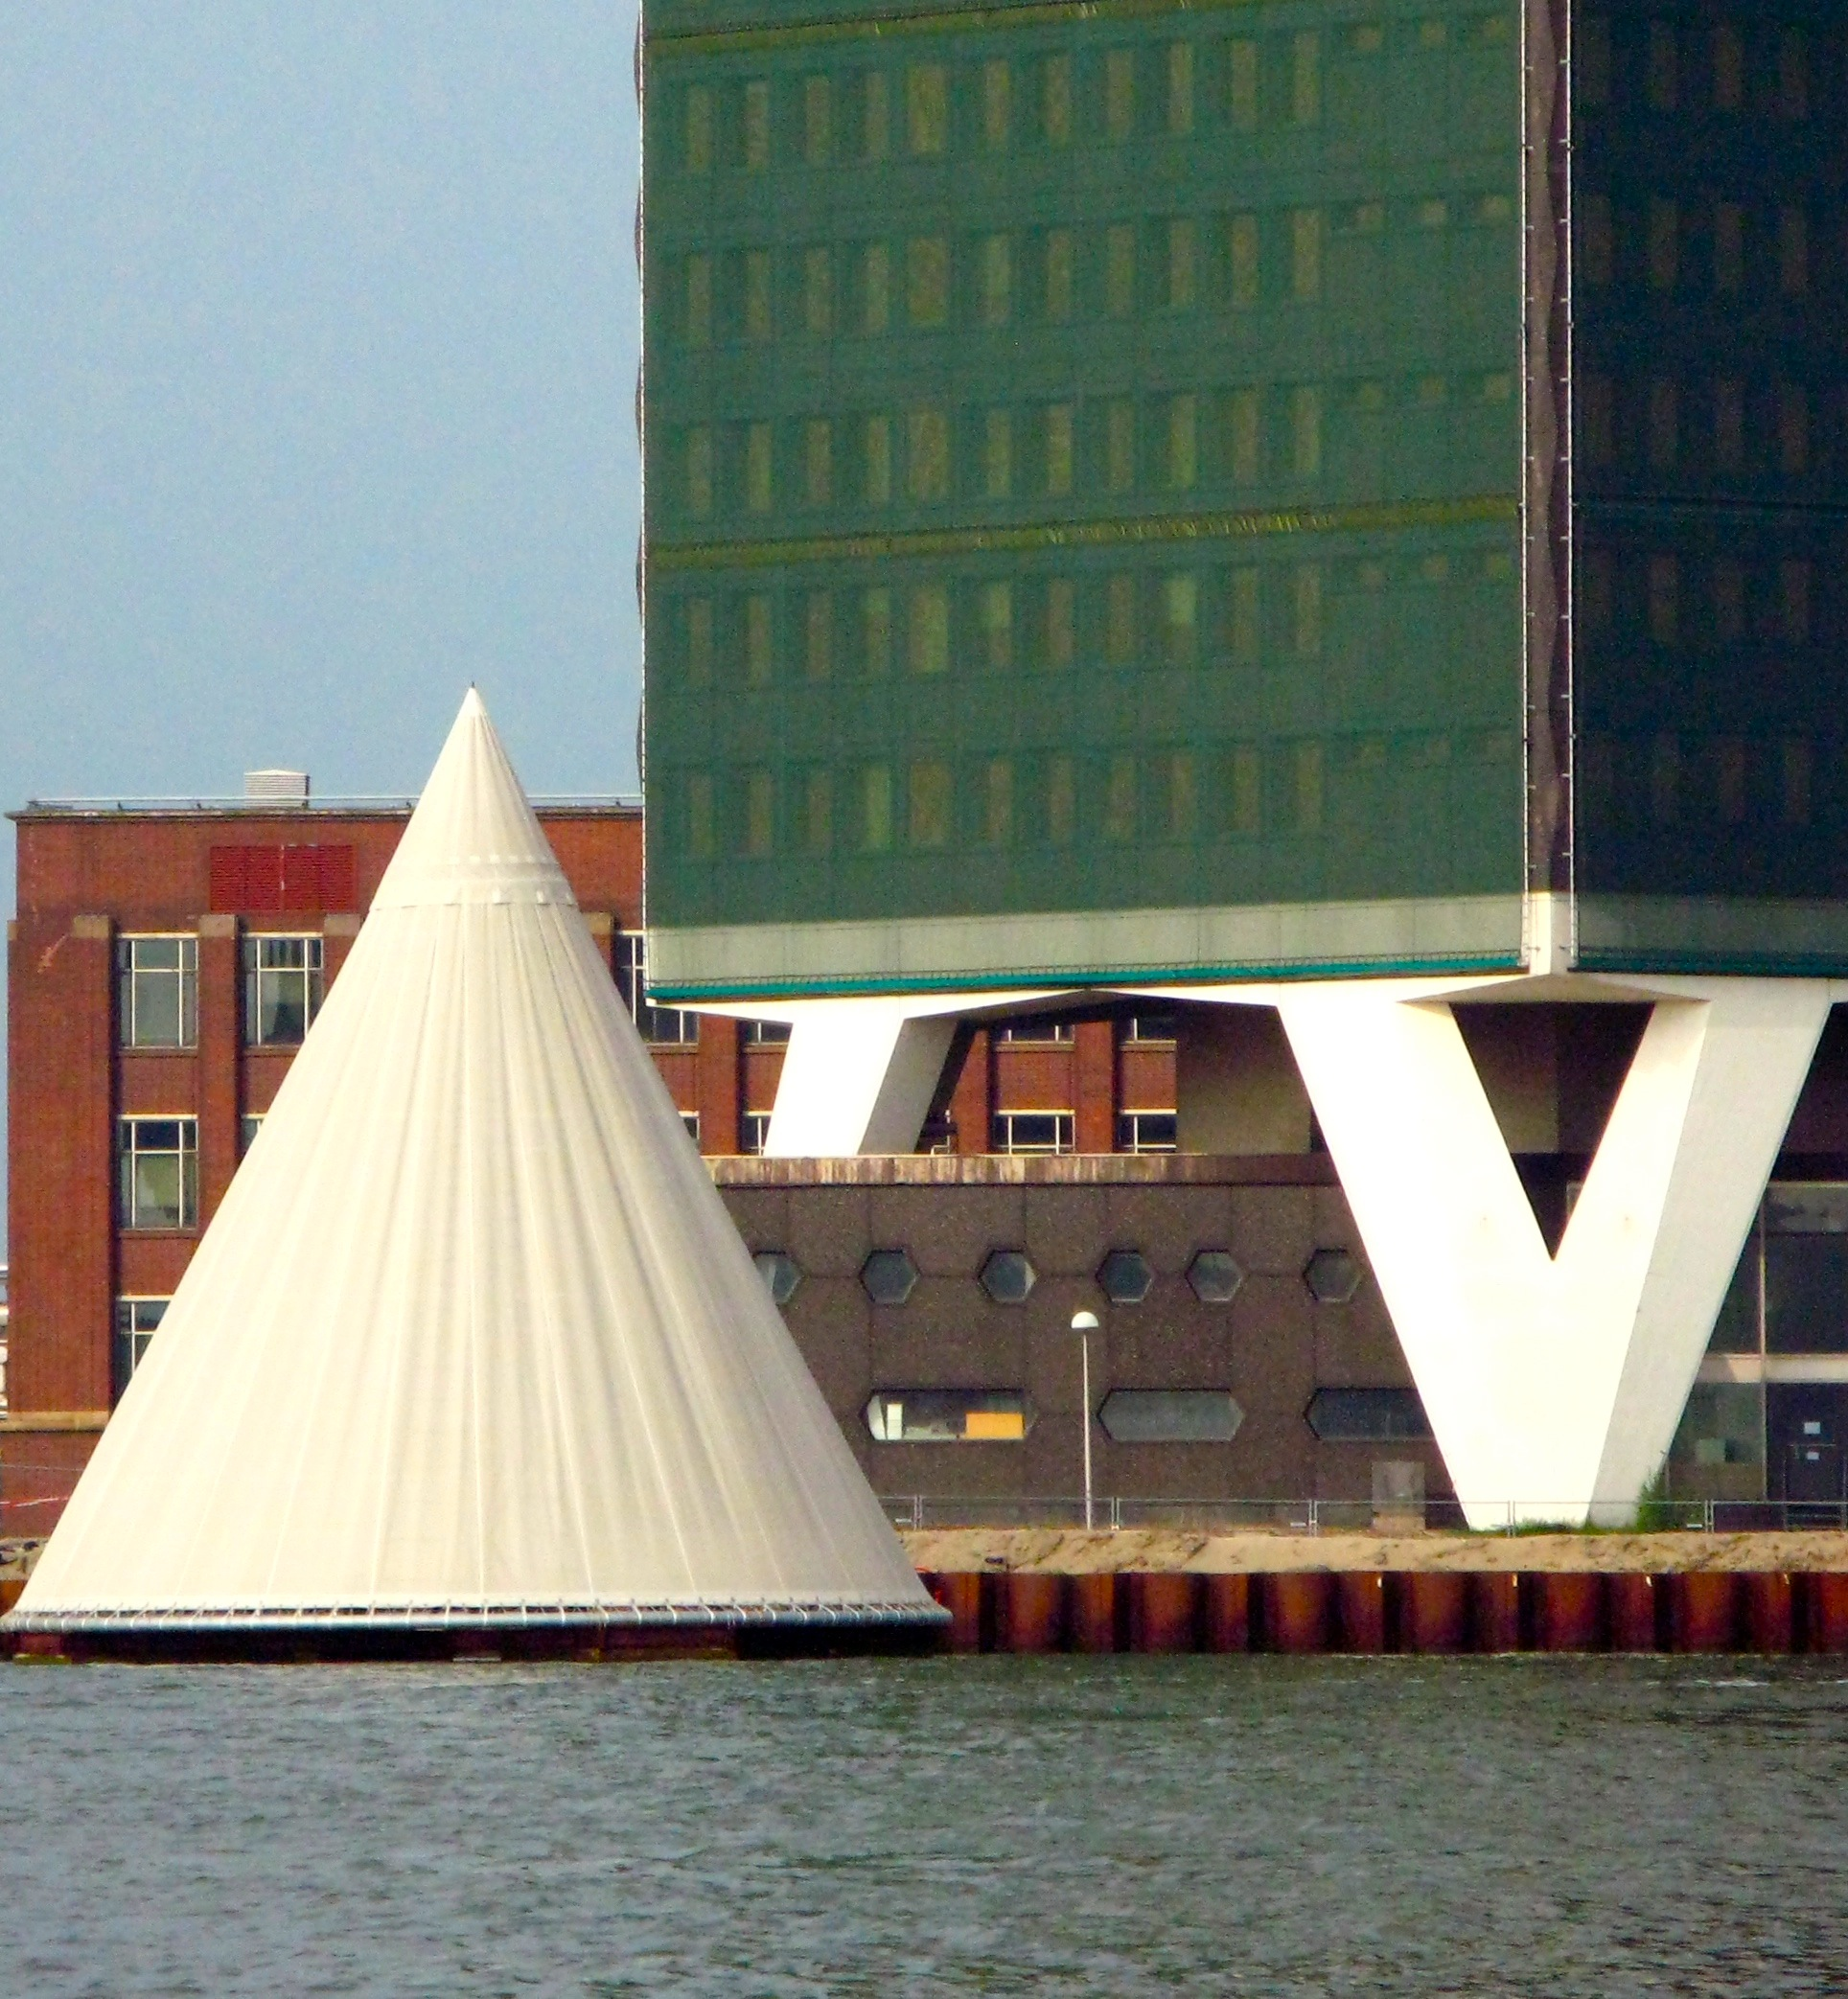
\includegraphics[width=0.95\textwidth]{geometry_lesson.jpg}
  \begin{center}
    {\large ``Geometry lesson''}\par
    Foto di kevindooley\par
    \url{http://www.flickr.com/photos/pagedooley/2575606606/}\par
    Licenza: Creative Commons Attribution\par
  \end{center}
\newpage

\section{Introduzione alla geometria razionale}
\subsection{Breve nota storica}
La parola geometria deriva dal greco antico: \textgreek{gewmetr'ia}, composta da \textgreek{gew} (geo) che significa ``terra'' e da \textgreek{metr'ia} (metria) che significa ``misura'', tradotto alla lettera significa ``misura della terra''. Secondo una tradizione storica, durante il VI secolo \aC{} alcuni matematici e pensatori greci (principalmente Talete e Pitagora) cominciarono a organizzare in maniera razionale (secondo il susseguirsi di ragionamenti logici) le conoscenze geometriche che egiziani e babilonesi avevano raggiunto nei secoli precedenti. Lo storico greco Erodoto, vissuto tra il 484 \aC{} e il 425 \aC, racconta che a causa delle periodiche inondazioni del fiume Nilo gli egiziani erano costretti a ricostruire ogni anno i confini dei singoli possedimenti terrieri e in questo modo avevano sviluppato delle modalità tecniche per la misura della terra (\textgreek{gewmetr'ia} appunto).

Ritrovamenti più recenti di tavolette di creta del periodo babilonese incise con caratteri cuneiformi ci fanno ritenere che la cultura babilonese possedesse già delle sofisticate conoscenze geometriche. Di certo sappiamo che nel III secolo \aC{} il matematico ellenico Euclide\footnote{vissuto molto probabilmente durante il regno di Tolomeo I (367 \aC{} ca. - 283 \aC).}, direttore della grande biblioteca di Alessandria in Egitto, diede una struttura razionale alle conoscenze geometriche note sino ad allora scrivendo una delle più grandi opere della cultura occidentale, gli \emph{Elementi} (in greco \textgreek{Stoiqeia}). Questa grande opera è organizzata in 13 libri, di cui i primi sei riguardano la Geometria Piana, i successivi quattro trattano i rapporti tra grandezze e gli ultimi tre riguardano la Geometria Solida. Essa prese il posto di tutti i libri precedenti sulla geometria e servì come testo fondamentale nell'antichità e nel medioevo; è stata usata come libro scolastico di geometria fino ai nostri giorni. La sua considerazione presso i Romani fu modesta, ma fu grandissima presso i Bizantini e gli Arabi. Proprio questi ultimi la reintrodussero in Europa dopo la perdita medievale, grazie alla traduzione di Adelardo di Bath\footnote{traduttore, filosofo e matematico britannico (1080 - 1152).} (secolo XII).

Dal punto di vista della struttura logica, gli \emph{Elementi} di Euclide sono organizzati a partire da cinque assiomi (nozioni comuni evidenti), cinque postulati (proposizioni che si richiede siano assunte come vere, senza dimostrazione) e 23 definizioni. L'opera di Euclide è rimasta nella nostra cultura l'unico punto di riferimento per lo studio della geometria, fino a quando, contestualmente allo studio dei fondamenti delle altre branche della matematica, i matematici cercarono di dare una base più rigorosa alla geometria di Euclide. Un'impostazione assiomatica più moderna venne data dal matematico tedesco David Hilbert\footnote{(1862 - 1943).} nel libro \emph{Grundlagen der Geometrie} (Fondamenti della geometria) pubblicato nel 1899, nel quale la geometria veniva fondata su ben 21 assiomi.

\subsection{Lo spazio fisico e la geometria}
La geometria nasce come studio sistematico dello spazio fisico e delle forme che in esso si muovono. Lo spazio in cui ci muoviamo è per tutti una delle prime esperienze che facciamo fin dai primi mesi di vita. I nostri sensi determinano le sensazioni che ci permettono di riconoscere le forme degli oggetti e i loro movimenti. Tuttavia, le nozioni geometriche come quelle di punto, retta, rettangolo, cubo, sfera \ldots non trovano un perfetto riscontro nella realtà fisica. Nello spazio fisico non esistono, infatti, punti e rette come li descrive la geometria, né figure a due sole dimensioni, né cubi o sfere perfette. La geometria si propone quindi di fornire un ``modello'' ideale della realtà fisica, sia per le forme degli oggetti sia per le proprietà dello spazio. 

Fino alla seconda metà dell'Ottocento, matematici e filosofi sono stati sostanzialmente d'accordo nel considerare la geometria come la scienza che descriveva razionalmente le proprietà dello spazio fisico. Galileo ne \emph{Il saggiatore} (1623) scriveva:
\begin{quoting}
La filosofia è scritta in questo grandissimo libro che continuamente ci sta aperto innanzi a gli occhi (io dico l'universo), ma non si può intendere se prima non s'impara a intender la lingua, e conoscer i caratteri, ne' quali è scritto. Egli è scritto in lingua matematica, e i caratteri son triangoli, cerchi, ed altre figure geometriche, senza i quali mezi è impossibile a intenderne umanamente parola; senza questi è un aggirarsi vanamente per un oscuro laberinto.
\end{quoting}
A partire dalla seconda metà del XIX secolo, i matematici si sono invece convinti che la geometria non descrive esattamente lo spazio fisico, che sono possibili più geometrie ugualmente vere dal punto di vista logico e matematico. Lo studio matematico della geometria si è allora differenziato dallo studio dello spazio fisico e da quello dello spazio psicologico percepito dall'uomo con i suoi sensi. I matematici hanno accettato l'esistenza di diverse geometrie matematicamente possibili, si sono accontentati di costruire dei modelli astratti e hanno lasciato ai fisici la ``scelta'' del modello che meglio si adatta a descrivere i fenomeni fisici dall'infinitamente piccolo all'infinitamente grande. La geometria allora è diventata una branca della matematica alla quale i matematici hanno cercato di dare un fondamento esclusivamente logico, indipendente dalle esperienze fisiche. 

Il legame tra fisica e matematica non si è mai rotto. Con il passare dei secoli, ci si è resi sempre più conto di quanto la ``geometria'' del mondo fisico sia molto complessa e di come alcune nuove geometrie riescono a descrivere meglio fenomeni che con la vecchia geometria di Euclide non si riusciva a spiegare.

\section{Il metodo assiomatico, i concetti primitivi e le definizioni}
La geometria, sin dai tempi di Euclide, è stata organizzata assiomaticamente, partendo cioè dalle fondamenta. Nella matematica queste fondamenta sono costituite dai concetti primitivi e dagli assiomi. Gli \emph{enti primitivi} sono le nozioni che si decide di non definire. Ci si può rendere facilmente conto, infatti, che non tutto può essere definito, poiché in ogni nozione che si definisce si deve fare ricorso ad altre nozioni, le quali a loro volta devono essere definite per mezzo di altre nozioni e così via all'indietro senza che teoricamente questo processo abbia mai una fine, arrivando necessariamente ad alcune nozioni così primitive da non poter essere definite con altre nozioni più elementari. A queste nozioni non è né necessario né possibile associare alcun significato esplicito; è invece fondamentale esprimere le loro proprietà esclusivamente attraverso \emph{assiomi}, cioè attraverso proprietà non dimostrabili che indicano però come gli enti primitivi devono e possono essere usati. Il matematico Hilbert utilizza tre enti primitivi -- punto, linea e piano -- e 21 assiomi. A partire dagli enti primitivi si fanno derivare tutte le \emph{definizioni} degli enti geometrici.

\subsection{Nozioni di logica}

Assumiamo come ``primitivo'' il concetto base di proposizione (o ``giudizio'' secondo la terminologia del grande filosofo greco Aristotele\footnote{(384 o 383 \aC{} - 322 \aC).}): chiamiamo \emph{proposizione} una frase (affermativa o negativa) a cui abbia senso associare un valore di verità, sia esso \emph{vero} (V) oppure \emph{falso} (F).

Per esempio, sono proposizioni logiche affermazioni del tipo <<Una retta ha infiniti punti>>, <<$2+3=10$>>. Non sono proposizioni logiche le frasi <<\np{1000} è un numero grande>>, <<il quadrato è semplice>>. Mentre la prima frase esprime un'affermazione vera e la seconda un'affermazione falsa, la terza e la quarta esprimono affermazioni non valutabili oggettivamente pertanto di queste ultime non si può dire se sono vere o false.

La logica delle proposizioni si fonda sui seguenti tre principi della logica aristotelica:
\begin{itemize*}
\item il \emph{principio di identità}: ogni oggetto è identico a se stesso e a nessun altro oggetto;
\item il \emph{principio di non contraddizione}: una stessa proposizione non può essere contemporaneamente vera e falsa;
\item il \emph{principio del terzo escluso}: una proposizione può essere solo vera o falsa, non può assumere un diverso valore di verità.
\end{itemize*}

Il corpo della geometria, come di qualunque altra teoria matematica, è costituito da \emph{proposizioni}, cioè da affermazioni che riguardano gli enti geometrici e che sono vere o false. Le proposizioni possono essere semplici affermazioni (\emph{proposizioni atomiche}) oppure possono essere ottenute da una o più proposizioni elementari legate tra di loro attraverso connettivi logici (elementi linguistici del tipo ``non'', ``e'', ``oppure'', ``o \ldots{} o'', ``quindi'', ``se \ldots{} allora'', ``se e solo se''). In questo caso si parla di \emph{proposizioni composte} o molecolari
Per esempio, la proposizione <<un triangolo ha tre lati e ha tre angoli>> è composta dalle proposizioni <<un triangolo ha tre lati>> e <<un triangolo ha tre angoli>> unite dal connettivo ``e''.

\paragraph{La congiunzione} di due proposizioni si ottiene con il connettivo ``e'' (\emph{et}, \emph{and}, $\wedge$): la proposizione $r$ ottenuta dalla congiunzione delle proposizioni $p$ e $q$, in simboli può essere scritta come
\begin{empheq}[box=\fbox]{equation*}
\vphantom{I}r=p\wedge q
\end{empheq}
ed è vera se entrambe le proposizioni $p$ e $q$ sono contestualmente vere, mentre è falsa quando anche una sola delle due proposizioni è falsa.
Per esempio, <<ho avuto 7 in italiano e matematica>> è un'affermazione vera solo quando ho avuto 7 in entrambe le materie e falsa in tutti gli altri casi.

Per esprimere in maniera sintetica tutte le possibilità del valore di verità di una proposizione composta, si usa una tabella a doppia entrata, detta \emph{tavola di verità}, che per la congiunzione logica è la seguente
\begin{center}
 \begin{tabular*}{.25 \textwidth}{@{\extracolsep{\fill}}*{3}{c}}
 \toprule
~$p$ &~$q$ &~$p\wedge q$\\
\midrule
~V & V & V \\
~V & F & F \\
~F & V & F \\
~F & F & F \\
\bottomrule
 \end{tabular*}
\end{center}

\paragraph{La disgiunzione (inclusiva)} di due proposizioni si ottiene con il connettivo ``o'' (\emph{vel}, \emph{or}, ${\vee}$): la proposizione $s$ ottenuta dalla disgiunzione di due proposizioni $p$ e $q$, in simboli
\begin{empheq}[box=\fbox]{equation*}
\vphantom{I}s=p\vee q
\end{empheq}
è vera quando almeno una delle due proposizioni è vera ed è falsa solo se entrambe le proposizioni sono false.
\begin{center}
 \begin{tabular*}{.25 \textwidth}{@{\extracolsep{\fill}}*{3}{c}}
 \toprule
~$p$ &~$q$ &~$p\vee q$\\
\midrule
~V & V & V \\
~V & F & V \\
~F & V & V \\
~F & F & F \\
\bottomrule
 \end{tabular*}
\end{center}

\paragraph{La negazione} di una proposizione si ottiene con il connettivo ``non'' (\emph{non}, \emph{not}, $\neg$), un operatore che, a differenza dei precedenti, non lega più proposizioni ma agisce su un'unica proposizione (per questo si dice che è un operatore unario, in analogia all'operazione insiemistica di complementazione). La proposizione $n$ data dalla negazione di una proposizione $p$ si indica con il simbolo
\begin{empheq}[box=\fbox]{equation*}
\vphantom{I}n=\neg p
\end{empheq}
ed è vera se $p$ è falsa, viceversa è falsa se $p$ è vera.

La doppia negazione equivale ad un'affermazione, cioè $\neg(\neg p)$ è equivalente a $p$.
La tavola di verità è la seguente:
\begin{center}
 \begin{tabular*}{.25 \textwidth}{@{\extracolsep{\fill}}*{3}{c}}
 \toprule
~$p$ &~$\neg p$ &~$\neg(\neg p)$\\
\midrule
~V & F & V \\
~F & V & F \\
\bottomrule
 \end{tabular*}
\end{center}

\paragraph{La disgiunzione esclusiva} di due proposizioni si ottiene con il connettivo [o congiunzione] ``o \ldots{} o'' (\emph{aut}, \emph{xor}, $\veebar$): la proposizione $t$ ottenuta dalla disgiunzione esclusiva di due proposizioni $p$ e $q$, in simboli
\begin{empheq}[box=\fbox]{equation*}
\vphantom{I}t=p\veebar q
\end{empheq}
è vera quando solo una delle due proposizioni è vera ed è falsa quando le due proposizioni sono entrambe vere o entrambe false.
Per esempio, nell'affermazione <<oggi il Milan vince o pareggia>> la congiunzione ``o'' ha valore esclusivo.

La disgiunzione esclusiva $\veebar$ a volte non viene messa tra gli operatori logici fondamentali perché è esprimibile attraverso gli altri tre operatori presentati finora.
\begin{center}
 \begin{tabular*}{.25 \textwidth}{@{\extracolsep{\fill}}*{3}{c}}
 \toprule
~$p$ &~$q$ &~$p\veebar q$\\
\midrule
~V & V & F \\
~V & F & V \\
~F & V & V \\
~F & F & F \\
\bottomrule
 \end{tabular*}
\end{center}

\begin{exrig}
\begin{esempio}
Date le seguenti proposizioni $p=$~<<un triangolo ha tre lati>> (Vera), $q=$~<<un triangolo ha tre vertici>> (Vera), $r=$~<<un triangolo ha quattro angoli>> (Falsa), $s=$~<<un triangolo ha tre dimensioni>> (Falsa), allora:
\begin{itemize*}
\item $p\wedge q$ è vera,~~$q\wedge r$ è falsa,~~$r\wedge s$ è falsa;
\item $p\vee q$ è vera,~~$q\vee r$ è vera,~~$r\vee s$ è falsa;
\item $p\veebar q$ è falsa,~~$q\veebar r$ è vera,~~$r\veebar s$ è falsa.
\end{itemize*}
\end{esempio}
\end{exrig}

È piuttosto semplice capire il meccanismo della negazione se applicata a proposizioni atomiche, spesso è meno intuitivo il valore di verità della negazione di una proposizione più complessa.
Ad esempio, la negazione di $p\wedge q$ non è $\neg p\wedge \neg q$ bensì $\neg p\vee \neg q$, mentre la negazione di $p\vee q$ è $\neg p\wedge \neg q$ e non $\neg p\vee \neg q$.
In formule:
\begin{empheq}[box=\fbox]{equation*}
\vphantom{I}\neg (p\wedge q)= (\neg p)\vee (\neg q)\qquad\text{e}\qquad\neg (p\vee q)= (\neg p)\wedge (\neg q).
\end{empheq}

Per esempio, <<non è vero che Marco e Luca sono stati bocciati>> può voler dire che entrambi non sono stati bocciati o solo uno di loro non è stato bocciato.

Queste uguaglianze prendono il nome di \emph{leggi di De Morgan}\footnote{dal nome del matematico e logico britannico Augustuts De Morgan (1806 - 1871).}, e la loro verifica può essere effettuata con la seguente tavola di verità:
\begin{center}
 \begin{tabular*}{.8 \textwidth}{@{\extracolsep{\fill}}*{8}{c}}
 \toprule
~$p$ &~$q$ &~$ \neg p $&~$ \neg q $&~$p\wedge q$&~$\neg p\vee \neg q$&~$p\vee q$&~$\neg p\wedge \neg q$\\
\midrule
~V & V & F & F & V & F & V & F \\
~V & F & F & V & F & V & V & F \\
~F & V & V & F & V & V & V & F \\
~F & F & V & V & F & V & F & V \\
\bottomrule
 \end{tabular*}
\end{center}

Come per le operazioni aritmetiche anche per gli operatori logici è possibile analizzarne le proprietà. Ne indichiamo qualcuna a titolo di esempio:
\begin{itemize*}
\item $(p\wedge q)\wedge r= p\wedge (q\wedge r)$ proprietà \emph{associativa} della congiunzione;
\item $p\wedge q= q\wedge p$ proprietà \emph{commutativa} della congiunzione;
\item $p\wedge (q\vee r)= (p\wedge q)\vee (p\wedge r)$ proprietà \emph{distributiva} della congiunzione rispetto alla disgiunzione.
\end{itemize*}

Una proposizione che è sempre vera indipendentemente dalla verità degli elementi che lo compongono è detta \emph{tautologia}. Una proposizione che è sempre falsa indipendentemente dalla verità dei suoi elementi è invece detta \emph{contraddizione}.

Per esempio, la proposizione composta $p\wedge \neg p$ è una contraddizione in quanto è sempre falsa, mentre la proposizione composta $p\vee \neg p$ è una tautologia poiché è sempre vera.

\vspazio\ovalbox{\risolvii \ref{ese:1.1}, \ref{ese:1.2}, \ref{ese:1.3}, \ref{ese:1.4}, \ref{ese:1.5}, \ref{ese:1.6}, \ref{ese:1.7}, \ref{ese:1.8}, \ref{ese:1.9}, \ref{ese:1.10}, \ref{ese:1.11}}


\subsection{Predicati e quantificatori}

Una proposizione che fa riferimento a una proprietà o caratteristica di alcuni elementi di un insieme si chiama \emph{predicato} (o \emph{enunciato}). Le frasi formate da un predicato che ha alcuni argomenti incogniti si dicono \emph{enunciati aperti}.
Per esempio, $p=$~<<$x$ è un numero intero maggiore di 10>> è un enunciato aperto.

Consideriamo ora le seguenti affermazioni:
\begin{itemize*}
\item <<tutti gli uomini sono mortali>> si riferisce a un qualsiasi essere umano;
\item <<tutti i multipli di 6 sono anche multipli di 2>> è vera per tutti i numeri multipli di 6;
\item <<ogni numero negativo è minore di ogni numero positivo>>.
\end{itemize*}
I predicati precedenti non riguardano un elemento specifico ma una certa quantità di elementi. I termini ``tutti'' e ``ogni'', detti \emph{quantificatori universali}, indicano che una proprietà è vera per tutti gli elementi di un certo insieme. In logica matematica per indicare il quantificatore universale si usa il simbolo $\forall$, che si legge ``per ogni''.

Vediamo ora i seguenti predicati:
\begin{itemize*}
\item <<esiste un numero che elevato al quadrato dà $16$>>;
\item <<alcuni numeri pari sono anche multipli di $3$>>.
\end{itemize*}
Queste affermazioni esprimono proprietà che sono vere almeno per un elemento dell'insieme di riferimento: la prima frase è vera per i numeri $+4$ e $-4$, la seconda frase è vera per i numeri $6$, $12$, $18$, \ldots{}
I termini ``c'è almeno'', ``alcuni'', ``esiste almeno uno'' si dicono \emph{quantificatori esistenziali} ed in logica matematica si indicano con il simbolo $\exists$, che si legge ``esiste''.

Bisogna prestare particolare attenzione quando si negano frasi in cui compaiono i quantificatori. Per esempio la negazione di <<tutti i gatti fanno le fusa>> non è <<nessun gatto fa le fusa>> bensì <<non tutti i gatti fanno le fusa>> che si può esprimere anche con il quantificatore esistenziale <<C'è almeno un gatto che non fa le fusa>>.
La negazione della frase <<l'anno scorso siamo stati tutti promossi>> non è <<l'anno scorso siamo stati tutti bocciati>> ma <<l'anno scorso non siamo stati tutti promossi>> ovvero <<l'anno scorso c'è stato almeno uno di noi che non è stato promosso>>.
La negazione della proposizione $p=$~<<tutti i quadrati hanno due diagonali>> è la proposizione ${\lnot}p=$~<<non tutti i quadrati hanno due diagonali>>.
Il linguaggio comune ci potrebbe portare a considerare come negazione di $p$ la proposizione <<nessun quadrato ha due diagonali>>, in realtà per avere la negazione della proposizione $p$ basta che esista almeno un quadrato che non ha due diagonali.

\vspazio\ovalbox{\risolvii \ref{ese:1.12}, \ref{ese:1.13}, \ref{ese:1.14}}


\subsection{Implicazione}

Nel linguaggio matematico sono comuni proposizioni del tipo <<Se $p$ allora $q$>>. Ad esempio <<se un numero è multiplo di $12$ allora è multiplo di $3$>>. La frase precedente può essere espressa dicendo <<essere multiplo di $12$ \emph{implica} essere multiplo di $3$>>.

In logica frasi del tipo <<se $p$ allora $q$>> vengono tradotte utilizzando l'operatore $\Rightarrow$ detto \emph{implicazione}.
La scrittura <<se $p$ allora $q$>> si traduce quindi con la scrittura
\begin{empheq}[box=\fbox]{equation*}
\vphantom{I}p\Rightarrow q
\end{empheq}
che si legge ``$p$ implica $q$''.

La proposizione $p$ è detta \emph{antecedente}, (o \emph{ipotesi}) e la proposizione $q$ è detta \emph{conseguente} (o \emph{tesi}).
Il significato logico della proposizione $p\Rightarrow q$ è che <<tutte le volte che la proposizione $p$ è vera allora risulta vera anche la proposizione $q$>>. Ovvero non si specifica il caso in cui $p$ sia falsa.

Per esempio, l'affermazione <<se c'è il sole andiamo al mare>> è falsa solo quando c'è il sole e non andiamo al mare; l'affermazione, infatti, non dice nulla se il sole non c'è: quindi se non c'è il sole si è liberi di andare o non andare al mare. Anche l'affermazione <<se studi sarai promosso>> dice solo che se studi conseguirai la promozione, non dice nulla per il caso in cui tu non studi: in questo caso, infatti, potresti essere ugualmente promosso.

La tavola di verità è la seguente:
\begin{center}
 \begin{tabular*}{.25 \textwidth}{@{\extracolsep{\fill}}*{3}{c}}
 \toprule
~$p$ &~$q$ &~$p\Rightarrow q$\\
\midrule
~V & V & V \\
~V & F & F \\
~F & V & V \\
~F & F & V \\
\bottomrule
 \end{tabular*}
\end{center}

Uno degli errori logici più comuni è quello di pensare che da $p\Rightarrow q$ si possa dedurre  $\neg p\Rightarrow \neg q$.
Ad esempio dall'affermazione <<se piove prendo l'ombrello>> qualcuno può pensare che si possa dedurre <<se non piove non prendo l'ombrello>>. Riflettendoci, si intuisce che le due frasi non sono affatto consequenziali. Basta pensare che chi pronuncia la prima frase sta affermando che tutte le volte che piove prende naturalmente l'ombrello, ma non esclude la possibilità di prenderlo anche quando non piove (in effetti è saggio farlo se il cielo è coperto da nuvoloni neri!).

Così la frase (a) <<se $x$ è multiplo di $12$ allora è multiplo di $3$>> non vuol dire (b) <<se $x$ non è multiplo di $12$ allora non è multiplo di $3$>>.
Infatti la (a) è vera, mentre la (b) è falsa (si pensi ad esempio al numero $6$ che non è multiplo di $12$ ma è comunque multiplo di $3$).

Ciò che ragionevolmente si può dedurre da $p\Rightarrow q$ è $\neg q\Rightarrow \neg p$.
Ad esempio, da <<se $x$ è multiplo di $12$ allora è multiplo di $3$>> si può dedurre <<se $x$ non è multiplo di $3$ allora non è multiplo di $12$>>.

Data l'implicazione $p\Rightarrow q$, la proposizione $p$ viene detta \emph{condizione sufficiente} per $q$. Mentre la proposizione $q$ viene detta \emph{condizione necessaria} per $p$.
Per esempio, <<studiare>> è condizione necessaria per <<essere promossi>> ma non è sufficiente.
Quest'ultima espressione fa appunto riferimento al fatto che da $p\Rightarrow q$ si può dedurre  $\neg q\Rightarrow \neg p$. Ossia $q$ è necessaria per $p$ in quanto se non è vera $q$ non è vera neanche $p$.

Calcoliamo la tavola di verità di $p\Rightarrow q$ e di $\neg q\Rightarrow \neg p$ 
\begin{center}
 \begin{tabular*}{.6 \textwidth}{@{\extracolsep{\fill}}*{6}{c}}
 \toprule
~$p$ &~$q$ &~$p\Rightarrow q$ &~$ \neg q $ &~$ \neg p $&~$ \neg q\Rightarrow \neg p $ \\
\midrule
~V & V & V & F & F & V\\
~V & F & F & V & F & F\\
~F & V & V & F & V & V\\
~F & F & V & V & V & V\\
\bottomrule
 \end{tabular*}
\end{center}
Come si vede, le due proposizioni hanno gli stessi valori di verità.

In generale, data un'implicazione $p\Rightarrow q$ (\emph{proposizione diretta}):
\begin{itemize*}
\item l'implicazione $\neg p\Rightarrow \neg q$ si dice \emph{contraria} di $p\Rightarrow q$;
\item l'implicazione $q\Rightarrow p$ si dice \emph{inversa} di $p\Rightarrow q$;
\item l'implicazione $\neg q\Rightarrow \neg p$ si dice \emph{contronominale} (o \emph{controinversa}) di $p\Rightarrow q$.
\end{itemize*}

\paragraph{La doppia implicazione} o \emph{equivalenza logica} di due proposizioni $p$ e $q$ dà luogo a una proposizione che in simboli si rappresenta con
\begin{empheq}[box=\fbox]{equation*}
\vphantom{I}p\Leftrightarrow q
\end{empheq}
(leggasi ``$p$ se e solo se $q$'') che è vera solo se $p$ e $q$ sono entrambe vere o entrambe false. La tavola di verità è la seguente:
\begin{center}
 \begin{tabular*}{.75 \textwidth}{@{\extracolsep{\fill}}*{6}{c}}
 \toprule
~$p$ &~$q$ &~$p\Leftrightarrow q$ &~$ p\Rightarrow q $ &~$ q\Rightarrow p $&~$ (p\Rightarrow q)\wedge (q\Rightarrow p) $ \\
\midrule
~V & V & V & V & V & V\\
~V & F & F & F & V & F\\
~F & V & F & V & F & F\\
~F & F & V & V & V & V\\
\bottomrule
 \end{tabular*}
\end{center}
L'operatore $\Leftrightarrow $ è detto \emph{doppia implicazione} perché se vale $p\Leftrightarrow q$ allora valgono sia $p\Rightarrow q$ che $q\Rightarrow p$ (e viceversa). Nella tabella precedente, infatti, è stata messa in evidenza l'equivalenza logica tra la proposizione $p\Leftrightarrow q$ e la proposizione $(p\Rightarrow q)\wedge (q\Rightarrow p)$.

L'equivalenza logica è un relazione di equivalenza, infatti verifica le seguenti proprietà:
\begin{itemize*}
\item $p\Leftrightarrow p$: è \emph{riflessiva};
\item se $p\Leftrightarrow q$ allora vale anche $q\Leftrightarrow p$: è \emph{simmetrica};
\item se $p\Leftrightarrow q$ e $q\Leftrightarrow r$ allora vale anche $p\Leftrightarrow r$: è \emph{transitiva}.
\end{itemize*}

In matematica si usa spesso l'espressione <<$p$ è \emph{condizione necessaria e sufficiente} per $q$>>. Per esempio <<condizione necessaria e sufficiente affinché un numero sia divisibile per $3$ è che la somma delle sue cifre sia divisibile per $3$>>. Il significato della frase è che <<$p$ è sufficiente per $q$>> e inoltre <<$p$ è necessario per $q$>>. In altre parole significa che  $p\Rightarrow q$ e $q\Rightarrow p$. Nel caso dell'esempio vale quindi sia l'implicazione diretta, <<se un numero è divisibile per $3$ allora la somma delle sue cifre è divisibile per $3$>>, che quella inversa, <<se la somma delle cifre di un numero è divisibile per $3$ allora il numero stesso è divisibile per $3$>>.

\vspazio\ovalbox{\risolvii \ref{ese:1.15}, \ref{ese:1.16}, \ref{ese:1.17}}


\subsection{I teoremi}

Un \emph{teorema} è una proposizione composta del tipo  $I\Rightarrow T$, cioè una implicazione tra due proposizioni, dette \emph{ipotesi} ($I$) e \emph{tesi} ($T$).

Dimostrare un teorema significa fare un ragionamento logico che permetta di concludere che la tesi è vera avendo supposto che l'ipotesi sia vera. Nel caso in cui un teorema sia dimostrabile all'interno di una teoria, si dice che è un teorema valido.

In riferimento alla terminologia usata quando abbiamo parlato dell'implicazione, chiamiamo  $I\Rightarrow T$ \emph{teorema diretto}, $T\Rightarrow I$ \emph{teorema inverso}, $\neg I\Rightarrow \neg T$ \emph{teorema contrario} e $\neg T\Rightarrow \neg I$ \emph{teorema controinverso}. Ribadiamo l'equivalenza tra il teorema diretto ed il teorema controinverso, nonché l'equivalenza tra il teorema contrario ed il teorema inverso, mentre in generale la validità del teorema diretto non implica la validità del teorema inverso, e viceversa.

Nel caso particolare in cui vale sia $I\Rightarrow T$ che $T\Rightarrow I$, si scrive  $I\Leftrightarrow T$ e si dice che ipotesi e tesi sono \emph{logicamente equivalenti}. Più precisamente, nel linguaggio specifico delle scienze che fanno uso della logica, e quindi anche nel linguaggio della Geometria Razionale, se vale $I\Rightarrow T$, si dice che <<$I$ è condizione sufficiente per $T$>> e anche che <<$T$ è condizione necessaria per $I$>>; se in particolare vale  $I\Leftrightarrow T$, si usa dire che <<$I$ è condizione necessaria e sufficiente per $T$>>.

In generale incontreremo molti teoremi che vengono denominati genericamente \emph{proposizioni}, perché il nome di ``teorema'' viene tradizionalmente attribuito solo ai teoremi più importanti. Inoltre si usa chiamare \emph{lemma} una proposizione che non ha una grande importanza di per sé, ma che è particolarmente utile per la dimostrazione di altri teoremi. Si chiama invece \emph{corollario} un teorema importante che è una conseguenza immediata di un altro teorema.

Così come abbiamo visto che non è possibile definire tutto e che quindi bisogna assumere alcune nozioni come primitive, analogamente non è possibile dimostrare tutte le proposizioni di una teoria. Alcune proposizioni devono essere assunte come vere e costituiscono la base della dimostrazione dei teoremi; queste proposizioni si chiamano \emph{postulati} o \emph{assiomi}. Risulta evidente che cambiando sia pure uno solo degli assiomi cambiano anche i teoremi dimostrabili e quindi la teoria.

In generale, come abbiamo detto, dato un teorema (diretto) del tipo $p\Rightarrow q$, la sua validità non garantisce la validità del teorema inverso $q\Rightarrow p$. Questo però può succedere. In ogni caso, se sono vere $p\Rightarrow q$ e $q\Rightarrow p$, le due proposizioni sono \emph{logicamente equivalenti}, ossia $p\Leftrightarrow q$.
\begin{exrig}
\begin{esempio}
Teorema: <<un triangolo che ha i lati uguali ha anche gli angoli uguali>>.
\begin{itemize}
\item Il teorema si può schematizzare nel seguente modo: $p=$~<<un triangolo ha i lati uguali>>; $q=$~<<un triangolo ha gli angoli uguali>>. Il teorema enunciato è $p\Rightarrow q$.
\item  Il teorema inverso è  $q\Rightarrow p$, cioè <<un triangolo che ha gli angoli uguali ha anche i lati uguali>>.
\end{itemize}
In tale esempio sono validi sia il teorema diretto che quello inverso. Il fatto che uno dei due teoremi sia chiamato diretto e l'altro inverso è un fatto soggettivo, che può dipendere semplicemente dall'ordine con cui si enunciano i teoremi.
Il teorema precedente si può esporre allora nel seguente modo:
\item Teorema: <<un triangolo ha i lati uguali se e solo se ha gli angoli uguali>>.
\end{esempio}
\end{exrig}

\subsection{La deduzione}

Nel paragrafo precedente abbiamo parlato in modo generico di implicazione, deduzione, dimostrazione. Facciamo ora un po' di chiarezza sull'uso di questi termini. L'\emph{implicazione} è un'operazione tra proposizioni, mentre la \emph{deduzione} è il ragionamento logico che costituisce la base della dimostrazione di un teorema. Per l'implicazione materiale si usa il simbolo $\rightarrow$ mentre per la deduzione logica si usa il simbolo $\Rightarrow$.

La frase <<se 5 è un numero pari, allora il triangolo ha 4 lati>> è perfettamente valida dal punto di vista logico ed anzi è vera, poiché la premessa (proposizione antecedente) è falsa, per cui l'implicazione è vera anche se la proposizione conseguente è falsa (si tenga presente la tavola di verità di $p\Rightarrow q$).
Si noti però che la definizione di implicazione ha senso solamente se la premessa è vera, il suo ampliamento al caso in cui la premessa è falsa è motivata da ragioni di completezza della trattazione. Bisogna quindi fare attenzione ad usare l'implicazione logica quando la premessa è falsa. Teniamo comunque conto che se $p$ è falsa allora $(p\Rightarrow q)\wedge(p\Rightarrow \neg q)$ cioè $p\Rightarrow (q\wedge \neg q)$ è vera. Ma  $q\wedge \neg q$ è una contraddizione, quindi una premessa falsa implica sempre una contraddizione.

In realtà, la \emph{dimostrazione} di un teorema non è la verifica della validità dell'implicazione, anzi è un procedimento che fa uso della validità dell'implicazione stessa. In un teorema si parte dal supporre vera l'ipotesi e si dimostra, mediante un ragionamento logico che si basa sugli assiomi e su altri teoremi già dimostrati in precedenza, che anche la tesi è vera (questo se si segue il \emph{procedimento diretto}). Se si segue invece il \emph{procedimento indiretto} (o \emph{per assurdo}), si suppone che la tesi sia falsa e, sempre mediante ragionamento logico basato su assiomi e altri teoremi già dimostrati, si arriva ad affermare che l'ipotesi è falsa (cosa che non si deve accettare).

Le principali regole del corretto ragionamento seguono alcuni schemi particolari (detti \emph{sillogismi}, dal nome attribuito ad essi da Aristotele). Presentiamo qui i quattro principali sillogismi: il \emph{modus ponens}, il \emph{modus tollens}, il \emph{sillogismo disgiuntivo} e il \emph{sillogismo ipotetico}.
\begin{center}
 \begin{tabular*}{.8 \textwidth}{@{\extracolsep{\fill}}*{6}{c}}
 \toprule
 &Modus&Modus&\multicolumn{2}{c}{Sillogismo}&Sillogismo\\
 &ponens&tollens&\multicolumn{2}{c}{disgiuntivo}&ipotetico\\
\midrule
1\textsuperscript{a} premessa & $p\Rightarrow q$ & $p\Rightarrow q$ & $p\vee q$ & $p\vee q$ & $p\Rightarrow q$\\
2\textsuperscript{a} premessa & $ p $ & $ \neg q $ & $ \neg p $ & $ \neg q $  & $q\Rightarrow r$\\
\midrule
conclusione & $ q $ & $ \neg p $ & $ q $ & $ p $ & $p\Rightarrow r$\\
\bottomrule
 \end{tabular*}
\end{center}
Suggeriamo una lettura degli schemi appena esposti:
\begin{itemize*}
\item \emph{modus ponens}: se sappiamo che $p$ implica $q$ e che $p$ è vera, allora possiamo concludere che anche $q$ è vera (metodo diretto di dimostrazione);
\item \emph{modus tollens}: se sappiamo che $p$ implica $q$ e che $q$ è falsa, allora possiamo concludere che anche $p$ è falsa (metodo indiretto di dimostrazione);
\item \emph{sillogismo disgiuntivo}: se sappiamo che, tra $p$ e $q$, almeno una delle due è vera, e sappiamo che $p$ (rispettivamente $q$) è falsa, allora possiamo concludere che $q$ (rispettivamente $p$) è vera;
\item \emph{sillogismo ipotetico}: se sappiamo che $p$ implica $q$ e che $q$ implica $r$, allora possiamo concludere che $p$ implica $r$ (proprietà transitiva dell'implicazione).
\end{itemize*}

Altre regole (note come i \emph{giudizi} di Aristotele) fanno uso dei predicati e dei quantificatori. Riprendiamo un esempio precedente traducendo la frase <<tutti i quadrati hanno due diagonali>> e la sua negazione <<non tutti i quadrati hanno due diagonali>> in formule che fanno uso anche del linguaggio degli insiemi. Se chiamiamo $Q$ l'insieme di tutti i quadrati e $P$ la proprietà dell'avere due diagonali, se $x$ è il generico quadrato (elemento di $Q$), $P(x)$ è il predicato <<$x$ gode della proprietà $P$>>, cioè <<$x$ ha due diagonali>>, la frase <<tutti i quadrati hanno due diagonali>> si traduce in simboli: ${\forall}x\in Q$, $P(x)$.

La sua negazione è: <<esiste almeno un quadrato che non ha due diagonali>>, cioè che non gode della proprietà $P$, e si traduce in simboli così: $\exists x\in Q$, $\neg P(x)$.
In quest'ultimo caso, la virgola può anche essere sostituita da una barra verticale (``\textbar'') o da ``:'' e si legge ``tale che''.

Analogamente, una frase del tipo <<esiste almeno un numero naturale che sia divisore di $10$>> può scriversi come: $\exists n\in\insN\mid D(n)$, dove $D$ è la proprietà dell'essere divisore di $10$ e $D(n)$ significa che $n$ verifica la proprietà $D$, cioè che $n$ è un divisore di $10$. La sua negazione è <<nessun numero naturale è divisore di 10>>, ovvero <<preso un qualsiasi numero naturale $n$, questo non gode della proprietà $D$>>, la traduzione in simboli di tale frase è: $\forall n\in\insN$, ${\neg}D(n)$.

Mettiamo in tabella le quattro proposizioni, che corrispondono ai giudizi di Aristotele):
%\begin{center}
% \begin{tabular*}{.8 \textwidth}{@{\extracolsep{\fill}}*{2}{l}}
% \multirow{2}*{A: Giudizio universale affermativo}&$\forall x\in Q$, $P(x)$\\
% & $P$ è vera per ogni $x$ \\
%\midrule
% \multirow{2}*{E: Giudizio universale negativo}&$\forall n\in\insN$, $\neg D(n)$\\
% & $D$ è falsa per ogni $n$ \\
%\midrule
% \multirow{2}*{I: Giudizio particolare positivo}&$\exists n\in\insN\mid D(n)$\\
% & $D$ è vera per almeno un $n$ \\
%\midrule
% \multirow{2}*{O: Giudizio particolare negativo}&$\exists x\in Q\mid\neg P(x)$\\
% & $P$ è falsa per almeno un $x$ \\
% \end{tabular*}
%\end{center}
\begin{center}
 \begin{tabular}{cc|cc}
 \toprule
 \multirow{3}{2.5cm}{A: Giudizio universale affermativo}&$\forall x\in Q$, $P(x)$&\multirow{3}{2.5cm}{I: Giudizio particolare affermativo}&$\exists n\in\insN\mid D(n)$\\
&\multirow{2}*{$P$ è vera per ogni $x$}& &\multirow{2}*{$D$ è vera per almeno un $n$}\\
&&&\\
\midrule
 \multirow{3}{2.5cm}{E: Giudizio universale negativo}&$\forall n\in\insN$, $\neg D(n)$&\multirow{3}{2.5cm}{O: Giudizio particolare negativo}&$\exists x\in Q\mid\neg P(x)$\\
 &\multirow{2}*{$D$ è falsa per ogni $n$}& &\multirow{2}*{$P$ è falsa per almeno un $x$}\\
 &&&\\
 \bottomrule
 \end{tabular}
\end{center}
I quattro giudizi di Aristotele si possono rappresentare con gli insiemi di Venn (figura~\ref{fig:1.1}).
\begin{figure}[bth]
 \centering% (c) 2014 Daniele Masini - d.masini.it@gmail.com
\begin{tikzpicture}[scale=1,font=\small]
\usetikzlibrary{calc}


\begin{scope}
\coordinate (oy) at (0,0);
\coordinate (ox) at (.2,0);
\draw[red] (oy) circle (0.9);

\begin{scope}
\clip (ox) circle (0.5);
\draw[fill=orange!40,opacity=.4] (ox) circle (0.5);
\end{scope}

\draw[blue] (ox) circle (.5);
\node at(.2,0){$X$};
\node at(-.5,.4){$Y$};
\node at(0,1.2){$A$};
\node at(0,-1.3){Ogni $x$ è $y$};
\end{scope}

\begin{scope}[xshift=2.5cm]
\coordinate (ox) at (0,0);
\coordinate (oy) at (1.5,0);
\draw[blue] (ox) circle (0.65);
\draw[red] (oy) circle (0.65);
\node at(0,0){$X$};
\node at(1.5,0){$Y$};
\node at(0.75,1.2){$E$};
\node at(0.75,-1.3){Nessun $x$ è $y$};
\end{scope}

\begin{scope}[xshift=6cm]
\coordinate (ox) at (0,0);
\coordinate (oy) at (0.85,0);

\begin{scope}
\clip (ox) circle (0.7);
\draw[fill=orange!40,opacity=.4] (oy) circle (0.7);
\end{scope}

\draw[blue] (ox) circle (0.7);
\draw[red] (oy) circle (0.7);

\node at(-0.1,0){$X$};
\node at(0.95,0){$Y$};
\node at(0.425,1.2){$I$};
\node at(0.425,-1.3){Qualche $x$ è $y$};
\end{scope}

\begin{scope}[xshift=9cm]
\coordinate (ox) at (0,0);
\coordinate (oy) at (0.85,0);

\begin{scope}
\clip (ox) circle (0.7);
\draw[fill=orange!40,opacity=.4] (ox) circle (0.7);
\draw[fill=white] (oy) circle (0.7);
\end{scope}

\draw[blue] (ox) circle (0.7);
\draw[red] (oy) circle (0.7);

\node at(-0.1,0){$X$};
\node at(0.95,0){$Y$};
\node at(0.425,1.2){$O$};
\node at(0.425,-1.3){Qualche $x$ non è $y$};
\end{scope}



\end{tikzpicture}
 \caption{Rappresentazione con gli insiemi di Venn dei giudizi di Aristotele}\label{fig:1.1}
\end{figure}

\subsection{La dimostrazione}

Tenendo conto di quanto detto precedentemente, dimostrare che $I\Rightarrow T$ significa fare un ragionamento logico che permetta di concludere che la tesi $T$ è vera avendo supposto che l'ipotesi $I$ sia vera.

Quando attraverso un ragionamento logico, e cioè attraverso una catena di implicazioni del tipo  $I\Rightarrow A\Rightarrow B\Rightarrow \ldots{} \Rightarrow T$, si riesce a dedurre la verità di una proposizione $T$ a partire dalla verità di una proposizione $I$. Si dice che si è data una \emph{dimostrazione diretta} del teorema $I\Rightarrow T$ (attraverso le regole del modus ponens e del sillogismo ipotetico).

Un teorema può anche essere \emph{dimostrato per assurdo}, o con metodo \emph{indiretto}. Questo tipo di dimostrazione consiste nel partire dalla negazione di $T$ e, attraverso una catena di implicazioni, arrivare alla negazione di $I$ o, in generale, ad una contraddizione.

Esistono altri metodi di dimostrazione, di cui eventualmente si parlerà più diffusamente qualora si dovesse ricorrere ad essi. Per ora ci limitiamo a citarne un paio: \emph{dimostrazione per induzione} e \emph{dimostrazione mediante esempio} o \emph{controesempio}.

La \emph{dimostrazione per induzione} si usa in particolare quando vogliamo dimostrare una proprietà generale che vale per molte categorie di figure ma che non si può esprimere in maniera unica per tutte le categorie (ad esempio una proprietà che vale per tutti i poligoni ma che dipende dal numero dei lati, come l'estensione dei criteri di congruenza dei triangoli a poligoni di più lati).

Si usa invece un \emph{esempio} quando bisogna dimostrare che una certa proprietà vale per almeno un oggetto del nostro studio o un \emph{controesempio} per dimostrare che una proprietà non vale per tutti gli oggetti in esame.

Per fornire alcuni esempi di dimostrazione, avremmo bisogno di fissare prima i concetti di base e gli assiomi da cui partire, per cui rinviamo la questione al prossimo paragrafo.

Ma a cosa serve studiare la dimostrazione di un teorema? Perché non ci limitiamo ad elencare i teoremi? Per molte applicazioni basta in effetti conoscere il teorema e a volte anche soltanto la formula risolutiva. Tuttavia studiando le dimostrazioni si impara a dimostrare e quindi si impara a creare nuova matematica. Un altro importante vantaggio è che la dimostrazione spiega perché il teorema è vero e permette di scoprire la struttura nascosta nelle definizioni e nei teoremi.

Quando si studia una dimostrazione non bisogna limitarsi a leggerla e a impararla a memoria, occorre leggerla attivamente, ponendo attenzione su cosa si fa e cercando di anticipare i passaggi. Se un passaggio non è chiaro bisogna prima tornare indietro per capire come ci si è arrivati e quindi cercare di capire il motivo per cui l'autore ha messo quel passaggio. In generale, una dimostrazione va letta più volte smettendo solo quando la si è compresa a fondo.

\vspazio\ovalbox{\risolvii \ref{ese:1.35}, \ref{ese:1.18}}


\section{Gli enti fondamentali della geometria}

In questo paragrafo diamo un cenno del sistema assiomatico della geometria razionale facendo riferimento principalmente all'impostazione assiomatica di Hilbert.

\subsection{Concetti primitivi}

Sono concetti primitivi per la geometria il \emph{punto}, la \emph{retta} e il \emph{piano}. Di essi non si dà una definizione e costituiscono la base per definire tutti gli altri enti della geometria.

Oltre a questi tre enti primitivi occorre poi assumere l'esistenza di tre relazioni primitive tra gli enti geometrici: \emph{giacere su}, \emph{stare fra}, \emph{essere congruente a}. Queste relazioni permettono di stabilire dei legami tra gli enti geometrici, per esempio: <<un punto giace su una retta>>, <<un punto sta fra altri due punti>>, <<un segmento è congruente a un altro segmento>>, \ldots

Esiste una simbologia convenzionale, condivisa dagli studiosi, per indicare questi enti:
\begin{itemize}
\item per indicare un punto usiamo una lettera maiuscola: $A$, $B$, $C$, \ldots;
\item per indicare una retta usiamo una lettera minuscola: $a$, $b$, $c$, \ldots;
\item per indicare un piano usiamo una lettera greca: $\alpha$, $\beta$, $\gamma$, \ldots
\end{itemize}

Ricordiamo l'alfabeto greco:
\begin{itemize}
\item lettere greche minuscole:  $\alpha$~(alfa),  $\beta$~(beta),  $\gamma$~(gamma),  $\delta$~(delta), $\epsilon$~(epsilon), $\zeta$~(zeta), $\eta$~(eta), $\theta$~(theta),  $\iota$~(iota),  $\kappa$~(kappa), $\lambda$~(lambda), $\mu$~(mi), $\nu$~(ni),  $\xi$~(xi), $o$~(omicron), $\pi$~(pi~o~pi~greca), $\rho$~(rho), $\sigma$~(sigma), $\tau$~(tau), $\upsilon$~(ipsilon), $\phi$~(fi), $\chi$~(chi), $\psi$~(psi), $\omega$~(omega);
\item lettere greche maiuscole: $A$, $B$, $ \Gamma $, $ \Delta $, $ E $, $ Z $, $ H $, $ \Theta $, $ I $, $ K $, $ \Lambda $, $ M $, $ N $, $ \Xi $, $ O $, $ \Pi $, $ \Sigma $, $ T $, $ \Upsilon $, $ \Phi $, $ X $, $ \Psi $, $\Omega $.
\end{itemize}

Degli enti fondamentali Euclide aveva dato le seguenti definizioni:
\begin{itemize*}
\item \emph{punto} è ciò che non ha parti;
\item \emph{linea} è lunghezza senza larghezza;
\item \emph{superficie piana} è quella che giace ugualmente rispetto alle rette su di essa.
\end{itemize*}
Le definizioni in questo caso sono utili per farci un'idea intuitiva degli enti stessi. Tuttavia, come è già stato detto in precedenza, e da quanto si intuisce osservando le definizioni euclidee, per definire il punto si utilizza la nozione di parte: ``punto è ciò che non ha parti''. Occorrerebbe quindi definire che cosa è una ``parte''. Ma per definire un parte avremmo bisogno di altre nozioni di partenza, in un procedimento senza fine. Per questo motivo nell'impostazione assiomatica moderna si preferisce non dare la definizione dei tre enti primitivi e ``definirli implicitamente'' attraverso le proprietà di cui godono. Ciò significa che si preferisce dare maggiore importanza a come essi si comportano e cosa possiamo fare con essi, piuttosto che descrivere cosa sono.
Dal punto di vista della rappresentazione grafica si usano le convenzioni come nella figura~\ref{fig:1.2}:
%\begin{center}
% \begin{tikzpicture}[font=\small]
%i punti
\tkzDefPoint(0,0){A}
\tkzDefPoint(1.5,1){B}
\tkzDefPoint(1,-1){C}
\tkzDrawPoints(A,B,C)
\tkzLabelPoints(A,B,C)
\node at(.75,-2){punti};

%le rette
\tkzDefPoint(3,-.5){D}
\tkzDefShiftPoint[D](30:1){E}
\tkzDefShiftPoint[D](30:3){F}
\tkzDefShiftPoint[D](30:4){G}
\tkzDrawSegments[style=dashed](D,E F,G)
\tkzDrawSegment(E,F)
\node at(4.3,.5){r};
\node at(4.3,-.5){s};

\tkzDefPoint(3,-1){D}
\tkzDefShiftPoint[D](35:1){E}
\tkzDefShiftPoint[D](35:3){F}
\tkzDefShiftPoint[D](35:4){G}
\tkzDrawSegments[style=dashed](D,E F,G)
\tkzDrawSegment(E,F)
\node at(4,-1-1){rette};

%il piano
\tkzDefPoint(6,-1){H}
\tkzDefShiftPoint[H](60:2.5){I}
\tkzDefShiftPoint[I](0:3){L}
\tkzDefShiftPoint[H](0:3){M}
\tkzDrawPolygon[fill=blue!10](H,I,L,M)
\node at(7.5,-1-1){piano};
\node at(10.3,.7){$\pi$};

\end{tikzpicture}

%\end{center}
\begin{figure}[htb]
 \centering\begin{tikzpicture}[font=\small]
%i punti
\tkzDefPoint(0,0){A}
\tkzDefPoint(1.5,1){B}
\tkzDefPoint(1,-1){C}
\tkzDrawPoints(A,B,C)
\tkzLabelPoints(A,B,C)
\node at(.75,-2){punti};

%le rette
\tkzDefPoint(3,-.5){D}
\tkzDefShiftPoint[D](30:1){E}
\tkzDefShiftPoint[D](30:3){F}
\tkzDefShiftPoint[D](30:4){G}
\tkzDrawSegments[style=dashed](D,E F,G)
\tkzDrawSegment(E,F)
\node at(4.3,.5){r};
\node at(4.3,-.5){s};

\tkzDefPoint(3,-1){D}
\tkzDefShiftPoint[D](35:1){E}
\tkzDefShiftPoint[D](35:3){F}
\tkzDefShiftPoint[D](35:4){G}
\tkzDrawSegments[style=dashed](D,E F,G)
\tkzDrawSegment(E,F)
\node at(4,-1-1){rette};

%il piano
\tkzDefPoint(6,-1){H}
\tkzDefShiftPoint[H](60:2.5){I}
\tkzDefShiftPoint[I](0:3){L}
\tkzDefShiftPoint[H](0:3){M}
\tkzDrawPolygon[fill=blue!10](H,I,L,M)
\node at(7.5,-1-1){piano};
\node at(10.3,.7){$\pi$};

\end{tikzpicture}

 \caption{Rappresentazione grafica degli enti fondamentali della geometria}\label{fig:1.2}
\end{figure}

\vspazio\ovalbox{\risolvi \ref{ese:1.32}}

\subsection{Postulati}

Un \emph{postulato}, o \emph{assioma}, è una proposizione, spesso intuitiva, evidente ma non dimostrata, ammessa come vera in quanto necessaria per costruire poi le dimostrazioni dei teoremi.

Euclide nei suoi \emph{Elementi} aveva individuato un gruppo di cinque assiomi, che riguardano le nozioni comuni e quindi non fanno riferimento alla geometria, e un gruppo di cinque postulati che riguardano proprietà geometriche.

\paragraph{Assiomi di Euclide}
\begin{enumerate}[label=\Roman{*}.]
\item Cose che sono uguali a una stessa cosa sono uguali anche tra loro.
\item Se cose uguali sono addizionate a cose uguali, le totalità sono uguali.
\item Se da cose uguali sono sottratte cose uguali, i resti sono uguali.
\item Cose che coincidono fra loro sono uguali.
\item Il tutto è maggiore della parte.
\end{enumerate}

\paragraph{Postulati di Euclide}
\begin{enumerate}[label=\Roman{*}.]
\item Si possa condurre una linea retta da un qualsiasi punto ad ogni altro punto.
\item Un segmento si possa prolungare indefinitamente in linea retta.
\item Si possa descrivere un cerchio con qualsiasi centro e qualsiasi raggio.
\item Tutti gli angoli retti siano uguali tra loro.
\item Se una retta che taglia due rette forma dallo stesso lato angoli interni la cui somma è minore di due angoli retti, prolungando illimitatamente le due rette, esse si incontreranno dalla parte dove i due angoli sono minori di due retti.

\begin{minipage}{.49\textwidth}
\centering% (c) 2014 Daniele Masini - d.masini.it@gmail.com
\begin{tikzpicture}[scale=1,font=\small]
\usetikzlibrary{calc}


\begin{scope}
\coordinate (c1) at (0,0);
\coordinate (c2) at (4,0.7);
\coordinate (a1) at (1,-0.5);
\coordinate (a2) at (2.4,2);
\coordinate (b1) at (0.2,1.6);
\coordinate (b2) at (4,1.2);
\coordinate (ab) at (intersection of a1--a2 and b1--b2);
\coordinate (ac) at (intersection of a1--a2 and c1--c2);

\begin{scope}
\clip (b2) -- (ab) -- (ac) -- (c2) -- cycle;
\draw[blue, fill=blue!10] (ab) circle (0.3);
\draw[red, fill=red!10] (ac) circle (0.3);
\end{scope}

\draw (a1) -- (a2) node [left] {$a$};
\draw (b1) -- (b2) node [above] {$b$};
\draw (c1) -- (c2) node [below] {$c$};

\end{scope}


\end{tikzpicture}

\end{minipage}\hfil
\begin{minipage}{.45\textwidth}
Nella figura a lato, la retta $a$ taglia le rette $b$ e $c$, formando sul lato destro due angoli la cui somma è minore di due angoli retti. Prolungando opportunamente le rette $b$ e $c$, risulta che esse si incontrano sul lato destro della figura.
\end{minipage}
\end{enumerate}

Nell'impostazione assiomatica moderna di Hilbert, gli assiomi hanno la funzione di definire implicitamente gli enti primitivi, cioè di fissare le proprietà alle quali questi enti devono soddisfare. Hilbert aggiunge inoltre altri assiomi che Euclide stesso non aveva esplicitato chiaramente.

\subsubsection*{Assiomi di Hilbert}\label{sect:ass_Hilbert}

L'esposizione che segue è una semplificazione degli assiomi del grande matematico tedesco.\footnote{chi volesse studiare direttamente il testo originale può consultare \url{http://www.gutenberg.org/files/17384/17384-pdf.pdf} [ultima consultazione 20.03.2014].}

Hilbert assume come enti primitivi della geometria piana il \emph{punto} e la \emph{retta}, come relazioni primitive l'appartenenza di un punto ad una retta, il giacere di un punto tra altri due punti, e la congruenza di segmenti.

\paragraph{Assiomi di appartenenza} ``giacere su''
\begin{enumerate}[label=\Roman{*}.]
\item dati due punti distinti, esiste una e una sola retta che contiene entrambi i punti;
\item ogni retta contiene almeno due punti. Esistono almeno tre punti che non giacciono sulla stessa retta (figura~\ref{fig:1.3});
\item dati tre punti non allineati, esiste uno e un solo piano che contiene tutti e tre i punti. Ogni piano contiene almeno un punto (figura~\ref{fig:1.4});
\item se due punti di una retta giacciono su un piano, allora anche tutti gli altri punti della retta giacciono su questo piano (figura~\ref{fig:1.5});
\item se un punto giace su due piani distinti, allora esiste almeno un altro punto giacente su entrambi questi piani;
\item esistono almeno quattro punti che non giacciono sullo stesso piano.
\end{enumerate}

\begin{figure}[b,t,h]
 \begin{minipage}[b]{.32\textwidth}
 \centering
 \begin{tikzpicture}[font=\small]
%Assioma 2
\tkzDefPoint(0,0){O}
\tkzDefShiftPoint[O](20:.7){A}
\tkzDefShiftPoint[O](20:2){B}
\tkzDefShiftPoint[O](20:2.7){M}
\tkzDefShiftPoint[O](50:1.5){C}
\tkzDefShiftPoint[O](30:0){r}
\tkzDrawSegment(O,M)
\tkzDrawPoints(A,B,C)
\tkzLabelPoints[font=\small](A,B,C,r)
% % % % % % % % % % % % % % % % % % % % % % % % % % % % % % % % %
\begin{comment}
%i punti
\tkzDefPoint(0,0){D}
\tkzDefShiftPoint[D](60:2){G}
\tkzDefShiftPoint[G](0:2.5){F}
\tkzDefShiftPoint[D](0:2.5){E}
\tkzDrawPolygon[fill=blue!10](D,G,F,E)
\node at(3.6,1.4){$\pi$};

%le rette
\tkzDefPoint(.5,.5){H}
\tkzDefShiftPoint[H](30:.5){I}
\tkzDefShiftPoint[H](30:1.5){L}
\tkzDefShiftPoint[H](30:2){M}
\tkzDrawSegment(H,M)
\node at(4.3,.5){r};
\node at(4.3,-.5){s};

\tkzDefPoint(3,-1){D}
\tkzDefShiftPoint[D](35:1){E}
\tkzDefShiftPoint[D](35:3){F}
\tkzDefShiftPoint[D](35:4){G}
\tkzDrawSegments[style=dashed](D,E F,G)
\tkzDrawSegment(E,F)
\node at(4,-1-1){rette};
\end{comment}
% % % % % % % % % % % % % % % % % % % % % % % % % % % % % % % % %
\end{tikzpicture}

 \caption{Assioma II}\label{fig:1.3}
 \end{minipage}
 \begin{minipage}[b]{.32\textwidth}
 \centering
 \begin{tikzpicture}[font=\small]
%il piano1
\tkzDefPoint(0,0){D}
\tkzDefShiftPoint[D](60:2){G}
\tkzDefShiftPoint[G](0:2.5){F}
\tkzDefShiftPoint[D](0:2.5){E}
\tkzDrawPolygon[fill=blue!10](D,G,F,E)
\node at(3.6,1.4){$\pi$};
\tkzDefPoint(.9,1){A}
\tkzDefPoint(2.6,1.5){B}
\tkzDefPoint(2.1,.5){C}
\tkzDrawPoints(A,B,C)
\tkzLabelPoints[font=\small](A,B,C)
% % % % % % % % % % % % % % % % % % % % % % % % % % % % % % % % %
\begin{comment}
%i punti
\tkzDefPoint(.2,1){A}
\tkzDefPoint(1.3,1.7){B}
\tkzDefPoint(2.5,.5){C}
\tkzDrawPoints(A,B,C)
\tkzLabelPoints(A,B,C)
\node at(.75,-2){punti};

%le rette
\tkzDefPoint(3,-.5){D}
\tkzDefShiftPoint[D](30:1){E}
\tkzDefShiftPoint[D](30:3){F}
\tkzDefShiftPoint[D](30:4){G}
\tkzDrawSegments[style=dashed](D,E F,G)
\tkzDrawSegment(E,F)
\node at(4.3,.5){r};
\node at(4.3,-.5){s};

\tkzDefPoint(3,-1){D}
\tkzDefShiftPoint[D](35:1){E}
\tkzDefShiftPoint[D](35:3){F}
\tkzDefShiftPoint[D](35:4){G}
\tkzDrawSegments[style=dashed](D,E F,G)
\tkzDrawSegment(E,F)
\node at(4,-1-1){rette};
\end{comment}
% % % % % % % % % % % % % % % % % % % % % % % % % % % % % % % % %
\end{tikzpicture}

 \caption{Assioma III}\label{fig:1.4}
 \end{minipage}
 \begin{minipage}[b]{.32\textwidth}
 \centering
 \begin{tikzpicture}[font=\small]
%il piano1
\tkzDefPoint(0,0){D}
\tkzDefShiftPoint[D](60:2){G}
\tkzDefShiftPoint[G](0:2.5){F}
\tkzDefShiftPoint[D](0:2.5){E}
\tkzDrawPolygon[fill=blue!10](D,G,F,E)
\node at(3.6,1.4){$\pi$};
\tkzDefPoint(.5,.3){H}
\tkzDefShiftPoint[H](25:.7){A}
\tkzDefShiftPoint[H](25:2){B}
\tkzDefShiftPoint[H](25:2.7){M}
\tkzDefShiftPoint[H](35:2.5){r}
\tkzDrawSegment(H,M)
\tkzDrawPoints(A,B)
\tkzLabelPoints[font=\small](A,B,r)
% % % % % % % % % % % % % % % % % % % % % % % % % % % % % % % % %
\begin{comment}
%i punti
\tkzDefPoint(.2,1){A}
\tkzDefPoint(1.3,1.7){B}
\tkzDefPoint(2.5,.5){C}
\tkzDrawPoints(A,B,C)
\tkzLabelPoints(A,B,C)
\node at(.75,-2){punti};

%le rette
\tkzDefPoint(.5,.5){H}
\tkzDefShiftPoint[H](30:.5){I}
\tkzDefShiftPoint[H](30:1.5){L}
\tkzDefShiftPoint[H](30:2){M}
\tkzDrawSegment(H,M)
\node at(4.3,.5){r};
\node at(4.3,-.5){s};

\tkzDefPoint(3,-1){D}
\tkzDefShiftPoint[D](35:1){E}
\tkzDefShiftPoint[D](35:3){F}
\tkzDefShiftPoint[D](35:4){G}
\tkzDrawSegments[style=dashed](D,E F,G)
\tkzDrawSegment(E,F)
\node at(4,-1-1){rette};
\end{comment}
% % % % % % % % % % % % % % % % % % % % % % % % % % % % % % % % %
\end{tikzpicture}

 \caption{Assioma IV}\label{fig:1.5}
 \end{minipage}
\end{figure}

\paragraph{Assiomi di ordinamento} ``stare fra''
\begin{enumerate}[label=\Roman{*}.]
\setcounter{enumi}{6}
\item Se un punto $B$ giace fra i punti $A$ e $C$, allora i punti $A$, $B$ e $C$ sono tre punti distinti sulla stessa retta, e $B$ giace fra $C$ ed $A$ (figura~\ref{fig:1.6});
\item dati due punti $A$ e $C$, esiste almeno un punto $B$, sulla retta $AC$, giacente fra di essi;
\item dati tre punti qualsiasi di una retta, uno e uno solo di essi giace fra gli altri due.
\end{enumerate}
Gli ultimi assiomi ci permettono di dedurre il seguente teorema.
\begin{teorema}
Tra due punti di una retta esiste sempre una quantità illimitata di altri punti.
\end{teorema}
\begin{proof}
Data una retta $r$ e due suoi punti $A$ e $B$, per l'assioma~VIII sappiamo che esiste un terzo punto $C$ sulla retta $r$ che giace tra $A$ e $B$. Ma allora esiste un punto $D$ su $r$ che giace tra $A$ e $C$ e un punto $E$ che giace tra $C$ e $B$. Per lo stesso assioma esisterà un punto tra $A$ e $D$, uno tra $D$ e $C$, uno tra $C$ e $B$ e così via.
\end{proof}
\begin{center}
\begin{tikzpicture}
%Assioma 14
\tkzDefPoint(0,0){L}
\tkzDefShiftPoint[L](0:.3){A}
\tkzDefShiftPoint[L](0:5.7){B}
\tkzDefShiftPoint[L](0:3){C}
\tkzDefShiftPoint[L](0:1.7){D}
\tkzDefShiftPoint[L](0:4.3){E}
\tkzDefShiftPoint[L](0:6){M}
\tkzDefShiftPoint[L](0:6){r}
\tkzDrawSegment(L,M)
\tkzDrawPoints(A,B,C,D,E)
\tkzLabelPoints[font=\small, above](A,B,C,D,E)
\tkzLabelPoint[font=\small](r){r}
\end{tikzpicture}

\end{center}
\begin{definizione}
Si chiama \emph{segmento} $AB$ l'insieme dei punti $A$ e $B$ e di tutti quelli che stanno sulla retta tra $A$ e $B$.
\end{definizione}
Gli assiomi di ordinamento ci permettono di dare anche la seguente

\begin{definizione}
Presi quattro punti $A$, $B$, $C$, $O$ su una retta, in modo che $B$ stia tra $A$ e $O$ e $O$ stia tra $A$ e $C$ possiamo dire che $A$ e $B$ \emph{stanno dalla medesima parte} rispetto a $O$, mentre $A$ e $C$ non stanno dalla medesima parte rispetto a $O$.
\end{definizione}
\begin{center}
\begin{tikzpicture}[scale=1,font=\small]
\usetikzlibrary{calc}

\begin{scope}
\coordinate (l) at (0,0);
\path (l) -- +(0:.5) coordinate (a);
\path (l) -- +(0:1.7) coordinate (b);
\path (l) -- +(0:5.3) coordinate (c);
\path (l) -- +(0:3) coordinate (o);
\path (l) -- +(0:4.3) coordinate (e);
\path (l) -- +(0:6.5) coordinate (m);

\draw (l) -- (m) node [above] {$r$};

\draw[fill] (a) circle (1pt) node [above] {$A$};
\draw[fill] (b) circle (1pt) node [above] {$B$};
\draw[fill] (c) circle (1pt) node [above] {$C$};
\draw[fill] (o) circle (1pt) node [above] {$O$};

\end{scope}

\end{tikzpicture}

\end{center}

\osservazione Trascuriamo in questa trattazione elementare l'assioma di Pasch\footnote{Moritz Pasch è stato un matematico tedesco (1843 - 1930).} (X) e l'assioma delle parallele (XI).

\paragraph{Assiomi di congruenza} ``essere congruente a''
\begin{enumerate}[label=\Roman{*}.]
\setcounter{enumi}{11}
\item \emph{Assioma del trasporto di un segmento}. Se $A$, $B$ sono due punti di una retta $r$ e $A'$ è un punto sulla stessa retta (o fissato su un'altra retta $r'$), si può sempre trovare un punto $B'$ sulla retta $r$ (o su $r'$), da una data parte rispetto ad $A'$, tale che il segmento $AB$ sia congruente al segmento $A'B'$;
\item la relazione di congruenza tra segmenti è transitiva, cioè se $A'B'$ è congruente ad $AB$ e $A''B''$ è congruente ad $AB$ allora $A'B'$ è congruente ad $A''B''$ (figura~\ref{fig:1.7});
\item siano $AB$ e $BC$ segmenti su una retta $r$ privi di punti comuni a parte $B$, e siano $A'B'$ e $B'C'$ segmenti su una retta $r'$ privi di punti comuni a parte $B'$. Se $AB\equiv A'B'$ e $BC\equiv B'C'$, allora  $AC\equiv A'C'$ (figura~\ref{fig:1.8}).
\end{enumerate}

\begin{figure}[b,t,h]
 \begin{minipage}[b]{.28\textwidth}
 \centering
 \begin{tikzpicture}
%Assioma 7
\tkzDefPoint(0,0){O}
\tkzDefShiftPoint[O](0:.5){A}
\tkzDefShiftPoint[O](0:1.2){B}
\tkzDefShiftPoint[O](0:1.9){C}
\tkzDefShiftPoint[O](0:2.5){M}
\tkzDefShiftPoint[O](0:2.5){r}
\tkzDrawSegment(O,M)
\tkzDrawPoints(A,B,C)
\tkzLabelPoints[font=\small, above](A,B,C)
\tkzLabelPoint[font=\small](r){$r$}
\end{tikzpicture}

 \caption{Assioma VII}\label{fig:1.6}
 \end{minipage}
 \begin{minipage}[b]{.34\textwidth}
 \centering
 \begin{tikzpicture}
%Assioma 12
\tkzDefPoint(0,0){L}
\tkzDefShiftPoint[L](0:.6){A}
\tkzDefShiftPoint[L](0:1.1){B}
\tkzDefShiftPoint[L](0:2){A'}
\tkzDefShiftPoint[L](0:2.5){B'}
\tkzDefShiftPoint[L](0:3){M}
\tkzDefShiftPoint[L](0:3){r}
\tkzDrawSegment(L,M)
\tkzDrawPoints(A,B,A',B')
\tkzLabelPoints[font=\small, above](A,B,A',B')
\tkzLabelPoint[font=\small](r){r}
\end{tikzpicture}

 \caption{Assioma XII}\label{fig:1.7}
 \end{minipage}
 \begin{minipage}[b]{.34\textwidth}
 \centering
 \begin{tikzpicture}
%Assioma 14
\tkzDefPoint(0,0){L}
\tkzDefShiftPoint[L](0:.6){A}
\tkzDefShiftPoint[L](0:1.5){B}
\tkzDefShiftPoint[L](0:2){C}
\tkzDefShiftPoint[L](0:3){M}
\tkzDefShiftPoint[L](0:3){r}
\tkzDrawSegment(L,M)
\tkzDrawPoints(A,B,C)
\tkzLabelPoints[font=\small, above](A,B,C)
\tkzLabelPoint[font=\small](r){r}

\tkzDefPoint(0,-.7){L}
\tkzDefShiftPoint[L](0:.6){A'}
\tkzDefShiftPoint[L](0:1.5){B'}
\tkzDefShiftPoint[L](0:2){C'}
\tkzDefShiftPoint[L](0:3){M}
\tkzDefShiftPoint[L](0:3){r'}
\tkzDrawSegment(L,M)
\tkzDrawPoints(A',B',C')
\tkzLabelPoints[font=\small, above](A',B',C')
\tkzLabelPoint[font=\small](r'){r'}
\end{tikzpicture}

 \caption{Assioma XIV}\label{fig:1.8}
 \end{minipage}
\end{figure}

Prima di proseguire con gli altri assiomi premettiamo le seguenti definizioni.
\begin{definizione}
Chiamiamo \emph{semiretta} la parte di retta costituita da un punto di essa, detto origine della semiretta, e da tutti i punti che stanno dalla stessa parte rispetto all'origine.
\end{definizione}

\begin{center}
 \begin{tikzpicture}
%Semiretta
\tkzDefPoint(0,0){O}
\tkzDefShiftPoint[O](0:5){C}
\tkzDefShiftPoint[O](0:6){M}
\tkzDrawSegment(O,C)
\tkzDrawSegment[style=dashed](C,M)
\tkzDrawPoint(O)
\tkzLabelPoint[font=\small, above](O){$O$}
\end{tikzpicture}

\end{center}

\begin{definizione}
Si dice \emph{angolo} ciascuna delle due parti in cui un piano è diviso da due semirette aventi l'origine in comune; le semirette si dicono \emph{lati} dell'angolo; l'origine comune alle due semirette si dice \emph{vertice} dell'angolo (figura~\ref{fig:1.9}).
\end{definizione}
\begin{figure*}[b,t,h]
\centering  \begin{tikzpicture}
%angolo1
\tkzDefPoint(0,0){H}
\tkzDefPoint(0,3){I}
\tkzDefShiftPoint[H](0:6){M}
\tkzDefShiftPoint[I](0:6){L}
\tkzDefPoint(2,1.5){V}
\tkzDefMidPoint(V,L)	\tkzGetPoint{M1}
\tkzDefMidPoint(V,M)	\tkzGetPoint{M2}
\tkzDrawSegments(V,L V,M)
\tkzFillPolygon[yellow!30](L,V,M,H,I)
\tkzFillPolygon[blue!30,opacity=.25](L,V,M)
%\tkzDrawSegment[style=dashed](C,M)
\tkzDrawPoint(V)
\tkzLabelPoint[above right](1,.3){Angolo}
\tkzLabelPoint[right](3.5,1.5){Angolo}
\tkzLabelPoint[font=\small, left](V){vertice}
\tkzLabelPoint[font=\small, above](V){V}
\tkzLabelPoint[font=\small, above](M1){lato}
\tkzLabelPoint[font=\small, below](M2){lato}
\tkzLabelPoint[font=\small, below left](L){r}
\tkzLabelPoint[font=\small, above left](M){s}
\end{tikzpicture}

\caption{Le semirette $r$ e $s$, aventi l'origine $V$ comune, individuano due regioni del piano ognuna delle quali è detta \emph{angolo}.}\label{fig:1.9}
\end{figure*}

L'angolo individuato da tre punti $A$, $B$, $C$ è l'angolo formato dalla semiretta con origine $B$ e passante per $A$ e dalla semiretta con origine $B$ e passante per $C$. Questo angolo si indica con il simbolo $A\widehat{B}C$. Nei disegni si usa indicare l'angolo con un archetto che indica la parte di piano considerata.

\begin{enumerate}[label=\Roman{*}.]
\setcounter{enumi}{14}
\item Dati un angolo $A\widehat{B}C$ ed una semiretta $B'C'$, esistono e sono uniche due semirette $B'D$ e $B'E$, tali che l'angolo $D\widehat{B'}C'$ è congruente all'angolo $A\widehat{B}C$ e l'angolo $E\widehat{B'}C'$ è congruente all'angolo $A\widehat{B}C$ (figura~\ref{fig:1.10});
\begin{figure}[b,t,h]
 \centering \begin{tikzpicture}
%assioma 15
\tkzDefPoint(0,0){B}
\tkzDefShiftPoint[B](0:2.5){A}
\tkzDefShiftPoint[B](0:3){I}
\tkzDefShiftPoint[B](30:2.5){C}
\tkzDefShiftPoint[B](30:3){H}
\tkzDrawPoints(A,B,C)
\tkzDrawSegments(B,H B,I)
\tkzLabelPoints[font=\small](B,C,A)
\tkzMarkAngle[fill=orange,opacity=.3,size=1cm](A,B,C)

\tkzDefShiftPoint[B](0:5){B'}
\tkzDefShiftPoint[B'](0:2.5){C'}
\tkzDefShiftPoint[B'](0:3){M}
\tkzDefShiftPoint[B'](30:2.5){E}
\tkzDefShiftPoint[B'](30:3){L}
\tkzDefShiftPoint[B'](-30:2.5){D}
\tkzDefShiftPoint[B'](-30:3){N}
\tkzDrawPoints(B',E,C',D)
\tkzDrawSegments(B',L B',M B',N)
\tkzLabelPoints[font=\small](E,C')
\tkzLabelPoints[font=\small,below](B',D)
\tkzMarkAngle[fill=orange,opacity=.3,size=1cm](D,B',C')
\tkzMarkAngle[fill=orange,opacity=.3,size=.9cm](C',B',E)

% % % % % %
\begin{comment}
\tkzDefShiftPoint[I](0:4){L}
\tkzDefPoint(1.5,1){V}
\tkzDefMidPoint(V,L)	\tkzGetPoint{M1}
\tkzDefMidPoint(V,M)	\tkzGetPoint{M2}
\tkzDrawSegments(V,L V,M)
\tkzFillPolygon[red!30,opacity=.25](L,V,M,H,I)
\tkzFillPolygon[blue!30,opacity=.25](L,V,M)
%\tkzDrawSegment[style=dashed](C,M)
\tkzDrawPoint(V)
\tkzLabelPoint[above right](.5,.1){Angolo}
\tkzLabelPoint[right](2.5,1){Angolo}
\tkzLabelPoint[font=\small, left](V){vertice}
\tkzLabelPoint[font=\small, above](V){V}
\tkzLabelPoint[font=\small, above](M1){lato}
\tkzLabelPoint[font=\small, below](M2){lato}
\tkzLabelPoint[font=\small, below left](L){r}
\tkzLabelPoint[font=\small, above left](M){s}
% % % % % % %
\end{comment}
\end{tikzpicture}

 \caption{Assioma XV}\label{fig:1.10}
\end{figure}
\item La relazione di congruenza tra angoli è transitiva, cioè se  $A'\widehat{B'}C'$ e  $A''\widehat{B''}C''$ sono congruenti ad $A\widehat{B}C$, allora  $A'\widehat{B'}C' \equiv A''\widehat{B''}C''$.
\end{enumerate}

\paragraph{Assioma di continuità}

\begin{enumerate}[label=\Roman{*}.]
\setcounter{enumi}{16}
\item \emph{Assioma di Archimede}. Sulla retta che unisce due punti qualsiasi $A$ e $B$ si prende un punto $A_1$, quindi si prendono i punti $A_2$, $A_3$, $A_4$, \ldots in modo che $A_1$ sia tra $A$ e $A_2$, $A_2$ tra $A_1$ e $A_3$, $A_3$ tra $A_2$ e $A_4$, ecc. e che  $AA_1\equiv A_1A_2\equiv A_2A_3\equiv A_3A_4\equiv\ldots$ allora tra tutti questi punti esiste sempre un punto $A_n$ tale che $B$ sta tra $A$ e $A_n$ (figura~\ref{fig:1.11}).
\begin{figure}[b,t,h]
 \centering \begin{tikzpicture}
%assioma 15
\tkzDefPoint(0,0){O}
\tkzDefShiftPoint[O](0:8){O'}
\tkzDefShiftPoint[O](0:5.1){B}
\tkzDefShiftPoint[O](0:1){A}
\tkzDefShiftPoint[O](0:1.9){A1}
\tkzDefShiftPoint[O](0:2.8){A2}
\tkzDefShiftPoint[O](0:3.7){A3}
\tkzDefShiftPoint[O](0:4.6){A4}
\tkzDefShiftPoint[O](0:5.5){A5}
\tkzDefShiftPoint[O](0:6.4){A6}
\tkzDefShiftPoint[O](0:7.4){A7}
\tkzDrawPoints(A1,A2,A3,A4,A5,A6,A7)
\tkzDrawPoints[fill=red,size=8](B,A)
\tkzDrawSegment(O,O')
\tkzLabelPoint[above](A){$A$}
\tkzLabelPoint[above](B){$B$}
\tkzLabelPoint[font=\small,above](A1){$A_1$}
\tkzLabelPoint[font=\small,above](A2){$A_2$}
\tkzLabelPoint[font=\small,above](A3){$A_3$}
\tkzLabelPoint[font=\small,above](A4){$A_4$}
\tkzLabelPoint[font=\small,above](A5){$A_5$}
\tkzLabelPoint[font=\small,above](A6){$A_6$}
\tkzLabelPoint[font=\small,above](A7){$A_7$}
\tkzLabelPoint[font=\small](7.8,0){$r$}
\end{tikzpicture}

 \caption{Assioma XVII di Archimede}\label{fig:1.11}
\end{figure}
\end{enumerate}

\paragraph{Assioma di completezza}

\begin{enumerate}[label=\Roman{*}.]
\setcounter{enumi}{17}
\item Ad un sistema di punti, linee rette e piani è impossibile aggiungere altri elementi in modo tale che il sistema, così generalizzato, formi una nuova geometria obbediente a tutti i cinque gruppi di assiomi. In altre parole, gli elementi della geometria formano un sistema che non è suscettibile di estensione, nel caso in cui si considerino validi i cinque gruppi di assiomi.
\end{enumerate}

\vspazio\ovalbox{\risolvii \ref{ese:1.33}, \ref{ese:1.34}, \ref{ese:1.36}, \ref{ese:1.37}, \ref{ese:1.38}, \ref{ese:1.39}, \ref{ese:1.40}, \ref{ese:1.41}, \ref{ese:1.42}}


\section{Prime definizioni}

\subsection{Semirette e segmenti}

Nel paragrafo precedente abbiamo già introdotto alcune definizioni di base, necessarie per enunciare tutti i postulati della geometria secondo l'assiomatizzazione di Hilbert. In questo paragrafo costruiamo le prime definizioni. Per comodità del lettore riportiamo anche quelle già date.

Partiamo dalla nozione generica di figura.
\begin{definizione}
Si chiama \emph{figura} un qualsiasi insieme, non vuoto, di punti.
\end{definizione}
Questa definizione fa riferimento soltanto all'ente primitivo geometrico di punto.

Lo spazio non è considerato un ente primitivo, in quanto può essere ottenuto dalla seguente definizione.
\begin{definizione}
Si chiama \emph{spazio} l'insieme di tutti i punti.
\end{definizione}
Risulta pertanto che una figura è un qualsiasi sottoinsieme dello spazio.

In base agli assiomi di ordinamento un qualunque punto $P$ su una retta divide la retta in due parti, una è costituita dai punti che ``seguono'' $P$, l'altra è costituita dai punti che ``precedono'' $P$.
\begin{definizione}
Si chiama \emph{semiretta} la parte di retta costituita da un punto di essa, detto origine della semiretta, e da tutti i punti che stanno dalla stessa parte rispetto all'origine.
\end{definizione}
Solitamente, la semiretta si indica con una lettera latina minuscola.

Prendendo due qualsiasi rette dello spazio esse si possono trovare in diverse posizioni reciproche, cioè una rispetto all'altra.
\begin{definizione}
Due rette che appartengono ad uno stesso piano si dicono \emph{complanari}, altrimenti si dicono \emph{sghembe}.
\end{definizione}

\begin{definizione}
Due rette complanari che non hanno nessun punto in comune si dicono \emph{parallele}.
\end{definizione}

\begin{definizione}
Due rette che hanno un solo punto in comune si dicono \emph{incidenti}.
\end{definizione}

\begin{definizione}
Se due rette hanno almeno due punti in comune sono \emph{coincidenti}.
\end{definizione}

\begin{figure}[hbt]
 \centering \begin{tikzpicture}[font=\small]
%rette coincidenti
\tkzDefPoint(0,0){A}
\tkzDefShiftPoint[A](20:3){B}
\tkzDefPoint(0,-.05){C}
\tkzDefShiftPoint[C](20:3){D}
\tkzLabelPoint[font=\small,above](B){$ r $}
\tkzLabelPoint[font=\small,below](D){$ s $}
\tkzDrawSegments(A,B C,D)
\node at(1.5,-1){$ r $ e $ s $ sono coincidenti};

%rette incidenti
\tkzDefPoint(3.5,0){A}
\tkzDefShiftPoint[A](20:3){B}
\tkzDefPoint(4,-.3){C}
\tkzDefShiftPoint[C](40:2.5){D}
\tkzLabelPoint[font=\small,below](B){$ v $}
\tkzLabelPoint[font=\small,above](D){$ u $}
\tkzDrawSegments(A,B C,D)
\node at(5,-1){$ u $ e $ v $ sono incidenti};

%rette parallele
\tkzDefPoint(7,0){A}
\tkzDefShiftPoint[A](30:3){B}
\tkzDefPoint(7.5,-.3){C}
\tkzDefShiftPoint[C](30:3){D}
\tkzLabelPoint[font=\small,above](B){$ m $}
\tkzLabelPoint[font=\small,below](D){$ n $}
\tkzDrawSegments(A,B C,D)
\node at(8.5,-1){$ m $ e $ n $ sono parallele};
\end{tikzpicture}

 \caption{Relazioni tra rette complanari}\label{fig:1.12}
\end{figure}
Per indicare che le rette $r$ e $s$ sono parallele si usa il simbolo $r \parallel s$.

\osservazione Due rette non parallele possono appartenere a piani diversi, in questo caso non avranno punti in comune, sono cioè sghembe. Viceversa se due rette hanno un punto in comune allora sono sicuramente complanari. Inoltre, se hanno più di un punto in comune le rette coincidono, in questo caso ci sono infiniti piani che le contengono. 

\begin{definizione}
L'insieme di tutte le rette di un piano che passano per uno stesso punto è detto \emph{fascio proprio di rette}, il punto in comune a tutte le rette si dice \emph{centro del fascio} (figura~\ref{fig:1.16}).
\end{definizione}

Prendendo due punti su una retta, $A$ e $B$, la retta resta divisa in tre parti: la semiretta di origine $A$ che non contiene $B$, la parte costituita dai punti compresi tra $A$ e $B$ e la semiretta di origine $B$ che non contiene $A$.

\begin{definizione}
Si chiama \emph{segmento} $AB$ l'insieme dei punti $A$ e $B$ e di tutti quelli che stanno tra $A$ e $B$.
I punti $A$ e $B$ si dicono \emph{estremi} del segmento.
\end{definizione}
Un segmento viene indicato con le due lettere maiuscole dei suoi estremi.
\begin{figure}[bth]
 \centering \begin{tikzpicture}[font=\small]
%definizione di segmento
\tkzDefPoint(0,0){r}
\tkzDefShiftPoint[r](0:9){s}
\tkzDefShiftPoint[r](0:3){A}
\tkzDefShiftPoint[r](0:6){B}
\tkzDefPoint(1.5,.5){e1}
\tkzDefPoint(7.5,.5){e2}
\tkzDefPoint(4.5,0){p}
\tkzDefPoint(1.5,-.5){s1}
\tkzDefPoint(7.5,-.5){s2}
\tkzDrawSegments[style=dashed](r,A B,s)
\tkzDrawSegment[very thick](A,B)
\tkzDrawPoints[fill=red](A,B)
\tkzLabelPoints[font=\small,above](r,s)
\tkzLabelPoints[font=\small,above](A,B)
\tkzLabelPoint[font=\small,above](p){punti interni}
\tkzLabelPoint[font=\small,below](4.5,-.5){segmento $AB$}
\tkzLabelPoint[font=\small,below](s1){semiretta di origine $A$}
\tkzLabelPoint[font=\small,below](s2){semiretta di origine $B$}
\tkzLabelPoint[font=\small,above](e1){estremo}
\tkzLabelPoint[font=\small,above](e2){estremo}
\tkzDrawSegments[thick,dotted,->,-latex](e1,A e2,B)
\tkzDrawSegment[thick,dotted,->,-latex]({4.5,-.5},{4.5,0})
%\draw[thick,dotted,->,-latex](0.5,-0.5).. controls (2,-.2)..(1,0);
%\draw[thick,dotted,->,-latex](8.5,-0.5).. controls (7,-.2)..(8,0);
\tkzDefPoint(1.5,0){rm}
\tkzDrawSegments[thick,dotted,->,-latex](s1,rm)
\tkzDefPoint(7.5,0){sm}
\tkzDrawSegments[thick,dotted,->,-latex](s2,sm)
\end{tikzpicture}

 \caption{I punti $A$ e $B$ formano le due semirette $r$ e $s$, e il segmento $AB$}\label{fig:1.13}
\end{figure}

Due segmenti nel piano possono trovarsi in diverse posizioni reciproche. Alcune di esse hanno un interesse per la geometria.
\begin{definizione}
Due segmenti si dicono \emph{consecutivi} se hanno in comune soltanto un estremo (figura~\ref{fig:1.14}).
\end{definizione}
\begin{figure}[bth]
 \centering % Copyright (c) 2015 Daniele Masini - d.masini.it@gmail.com

\begin{tikzpicture}[font=\small]
%segmenti consecutivi
\tkzDefPoint(0,0){B}
\tkzDefShiftPoint[B](120:2){A}
\tkzDefShiftPoint[B](0:2.5){C}
\tkzDrawPoints(A,B,C)
\tkzLabelPoints[font=\small](B,C)
\tkzLabelPoint[font=\small,right](A){A}
\tkzDrawSegments(A,B B,C)
\node at(1.25,-.7){segmenti consecutivi};

%non consecutivi
\tkzDefPoint(4,0){E}
\tkzDefShiftPoint[E](120:.7){F}
\tkzDefShiftPoint[E](120:2){D}
\tkzDefShiftPoint[F](10:2.5){G}
\tkzDrawPoints(E,F,D,G)
\tkzLabelPoints[font=\small,left](E,F,D)
\tkzLabelPoint[font=\small,above](G){G}
\tkzDrawSegments(E,D F,G)
\node at(6.5,-.7){Segmenti non consecutivi};

\tkzDefPoint(7,0){H}
\tkzDefShiftPoint[H](100:2){I}
\tkzDefShiftPoint[H](60:1.5){L}
\tkzDefShiftPoint[H](10:3){M}
\tkzDrawPoints(H,I,L,M)
\tkzLabelPoints[font=\small,right](H,I)
\tkzLabelPoints[font=\small,above](L,M)
\tkzDrawSegments(H,I L,M)
\end{tikzpicture}

 \caption{I segmenti $AB$ e $BC$ sono consecutivi perché hanno in comune solo il punto~$B$ che è un estremo di entrambi; $DE$ e $FG$ non sono consecutivi perché hanno in comune solo il punto $F$ ma esso non è estremo del segmento $DE$; $HI$ e $LM$ non sono consecutivi perché non hanno nessun punto in comune.}\label{fig:1.14}
\end{figure}

\begin{definizione}
Due segmenti si dicono \emph{adiacenti} se sono consecutivi ed appartengono alla stessa retta (figura~\ref{fig:1.15}).
\end{definizione}
\begin{figure}[tbh]
 \centering % Copyright (c) 2015 Daniele Masini - d.masini.it@gmail.com

\begin{tikzpicture}[font=\small]
%segmenti adiacenti
\tkzDefPoint(0,0){A}
\tkzDefShiftPoint[A](60:1.5){B}
\tkzDefShiftPoint[A](60:2.5){C}
\tkzDrawPoints(A,B,C)
\tkzLabelPoints[font=\small,right](A,B,C)
\tkzDrawSegment(A,C)
\node at(.3,-.5){segmenti adiacenti};

%non consecutivi
\tkzDefPoint(4,0){D}
\tkzDefShiftPoint[D](60:.7){E}
\tkzDefShiftPoint[D](60:1.7){F}
\tkzDefShiftPoint[D](60:2.5){G}
\tkzDrawPoints(E,F,D,G)
\tkzLabelPoints[font=\small,right](D,E,F,G)
\tkzDrawSegments(E,D F,G)
\tkzDrawSegment[dashed](E,F)
\node at(5.5,-.5){Segmenti non adiacenti};

\tkzDefPoint(7,0){H}
\tkzDefShiftPoint[H](60:1){L}
\tkzDefShiftPoint[H](60:1.5){I}
\tkzDefShiftPoint[H](60:2.5){M}
\tkzDrawPoints(H,I,L,M)
\tkzLabelPoints[font=\small,right](H,I,L,M)
\tkzDrawSegment(H,M)
\end{tikzpicture}

 \caption{I segmenti $AB$ e $BC$ sono adiacenti perché hanno in comune solo l'estremo $B$ e giacciono sulla stessa retta; i segmenti $DE$ e $FG$, pur giacendo sulla stessa retta, non sono adiacenti poiché non hanno alcun punto in comune; i segmenti $HI$ e $LM$ giacciono sulla stessa retta ma non sono adiacenti poiché hanno più di un punto in comune.}\label{fig:1.15}
\end{figure}

\ovalbox{\risolvii \ref{ese:1.43}, \ref{ese:1.44}, \ref{ese:1.45}, \ref{ese:1.46}, \ref{ese:1.47}, \ref{ese:1.48}, \ref{ese:1.49}, \ref{ese:1.50}}

\subsection{Semipiani e angoli}

\begin{definizione}
Si dice \emph{semipiano} di origine la retta $r$ la figura formata dalla retta $r$ e da una delle due parti in cui essa divide il piano (figura~\ref{fig:1.17}).
\end{definizione}
\begin{figure}[b,t,h]
 \begin{minipage}[b]{.40\textwidth}
 \centering\begin{tikzpicture}[font=/small]
\tkzDefPoint(0,0){O}
%\tkzDefPoint(2,0){A}
\foreach \ang in {30,60,...,360}{%
\tkzDefPoint(\ang:1.3){M}
\tkzDrawSegment(M,O)
}
\end{tikzpicture}

 \caption{Fascio proprio di rette}\label{fig:1.16}
 \end{minipage}\hfil
 \begin{minipage}[b]{.40\textwidth}
 \centering% (c) 2014 Daniele Masini - d.masini.it@gmail.com
\begin{tikzpicture}[font=\small]
%semipiani
\tkzDefPoint(0,0){D}
\tkzDefShiftPoint[D](50:2){G}
\tkzDefShiftPoint[G](0:2.5){F}
\tkzDefShiftPoint[D](0:2.5){E}
\tkzDefShiftPoint[D](50:.7){L}
\tkzDefMidPoint(F,E) \tkzGetPoint{M}
\tkzLabelPoint[right](M){$r$}
\tkzLabelPoint[right](F){$\pi$}
\tkzDrawPolygon[thin,blue,fill=blue!10](L,G,F,M)
\tkzDrawPolygon[thin,blue,fill=yellow!30](D,L,M,E)
\tkzDrawSegment[thick](L,M)
\node at(1.6,.3){semipiano};
\node at(2.1,1.2){semipiano};
\end{tikzpicture}

  \caption{Semipiani opposti}\label{fig:1.17}
  \end{minipage}
\end{figure}
In un piano ${\pi}$, una qualsiasi retta $r \subset \pi$ dà origine a due semipiani distinti, che si dicono semipiani \emph{opposti}.

\begin{definizione}
Una figura si dice \emph{convessa} se, considerati due suoi qualsiasi punti, il segmento che li unisce è contenuto nella figura. Si dice \emph{concava} se esistono almeno due punti per i quali il segmento che li unisce non è interamente contenuto nella figura (figura~\ref{fig:1.18}).
\end{definizione}
\begin{figure}[b,t,h]
 \centering \begin{tikzpicture}[font=\small]
%convesso
\tkzDefPoints{0/1/A,
1.4/.8/B,
3.5/2/C,
1.6/3.2/D,
.6/2/E}
\tkzDefShiftPoint[A](30:.5){A1}
\tkzDefShiftPoint[A1](40:2.1){D1}
\tkzDefShiftPoint[A1](5:.5){A2}
\tkzDefShiftPoint[A1](10:2.1){D2}
\tkzLabelPoint[below,font=\small](1.8,0.85){$F$}
%concavo
\tkzDefPoints{5/2.6/H,
5.8/3/I,
7/2/L,
8.2/2.8/M,
8.5/1.3/N,
8/.3/O,
7/.2/P,
6/.3/Q,
5/.8/R,
5.2/1.7/S}
\tkzDefShiftPoint[H](-3:.7){H1}
\tkzDefShiftPoint[M](-110:.6){M1}
\tkzDefShiftPoint[H](-60:.7){H2}
\tkzDefShiftPoint[L](-40:1){L1}
\tkzDefShiftPoint[R](-10:.5){Q1}
\tkzDefShiftPoint[Q1](10:2.5){Q2}
\tkzLabelPoint[below,font=\small](6.7,0.2){$G$}

\tkzDrawPolygon[fill=blue!10,rounded corners](A,B,C,D,E)
\tkzDrawPolygon[fill=yellow!30,rounded corners](H,I,L,M,N,O,P,Q,R,S)
\tkzDrawSegments(A1,D1 A2,D2 H1,M1 H2,L1 Q1,Q2)
\tkzDrawPoints(A1,D1,A2,D2,H1,M1,H2,L1,Q1,Q2)
\tkzLabelPoint[below,font=\small](H1){$P$}
\tkzLabelPoint[below,font=\small](M1){$Q$}

\end{tikzpicture}


 \caption{La figura $ F $ è convessa, per qualsiasi coppia di punti interni a $ F $ il segmento che li unisce è interamente nella figura; la figura $ G $ è concava perché unendo i punti $ P $ e $ Q $ si ha un segmento che cade in parte esternamente alla figura.}\label{fig:1.18}
\end{figure}

Ricordiamo la definizione di angolo già data: si dice \emph{angolo} ciascuna delle due parti in cui un piano è diviso da due semirette aventi l'origine in comune; le semirette si dicono \emph{lati} dell'angolo; l'origine comune alle due semirette si dice \emph{vertice} dell'angolo (figura~\ref{fig:1.9}).

\begin{definizione}
Un angolo si dice \emph{piatto} se i suoi lati sono uno il prolungamento dell'altro.
\end{definizione}

\begin{definizione}
Un angolo si dice \emph{nullo} se è costituito solo da due semirette sovrapposte.
\end{definizione}

\begin{definizione}
\`E detto \emph{angolo giro} l'angolo che ha per lati due semirette sovrapposte e che contiene tutti i punti del piano (figura~\ref{fig:1.19}).
\end{definizione}
\begin{figure}[bth]
 \centering \begin{tikzpicture}
%angolo piatto
\tkzDefPoint(0,0){a}
\tkzDefShiftPoint[a](0:3){b}
\tkzDefShiftPoint[a](0:1.5){V}
\tkzDefShiftPoint[B](30:2.5){C}
\tkzDefShiftPoint[B](30:3){H}
\tkzDrawPoints(a,V,b)
\tkzDrawSegment(a,b)
\tkzLabelPoints[font=\small,below](a,V,b)
\tkzMarkAngle[fill=orange,opacity=.3,size=.8cm](a,V,b)
\tkzMarkAngle[fill=blue!30,opacity=.3,size=.7cm](b,V,a)
\tkzLabelPoint[font=\small,above](1.5,.7){angolo piatto}
\tkzLabelPoint[font=\small,below](1.5,-.8){angolo piatto}
%angolo giro/nullo
\tkzDefShiftPoint[a](0:5){O}
\tkzDefPoint(5,.05){O1}
\tkzDefShiftPoint[O](0:2.5){c}
\tkzDefShiftPoint[O1](0:2.5){c1}
\tkzDefShiftPoint[O](-1:1.5){c2}
\tkzDrawPoint(O)
\tkzDrawSegments(O,c O1,c1)
\tkzLabelPoint[font=\small,above](5,.7){angolo giro}
\tkzLabelPoint[font=\small,below](6.7,0){angolo nullo}
\tkzMarkAngle[fill=orange,opacity=.3,size=.7cm](c,O,c2)
\end{tikzpicture}

 \caption{L'angolo  $\widehat{ab}$ a sinistra è piatto (sia quello sopra che quello sotto), gli angoli a destra, individuati dalle semirette coindicenti con origine in $O$, sono rispettivamente un angolo giro (quello esterno) e un angolo nullo (quello interno).}\label{fig:1.19}
\end{figure}

\begin{definizione}
Un angolo, i cui lati non appartengono alla stessa retta, si dice \emph{concavo} se contiene i prolungamenti dei lati, se non li contiene si dice \emph{convesso}.
\end{definizione}

\begin{figure*}[htb]
\centering  % (c) 2014 Daniele Masini - d.masini.it@gmail.com
\begin{tikzpicture}
%angolo1
\tkzDefPoint(0,0){H}
\tkzDefPoint(0,3){I}
\tkzDefShiftPoint[H](0:6){M}
\tkzDefShiftPoint[I](0:6){L}
\tkzDefPoint(2,1.5){V}
\tkzDefMidPoint(V,L)	\tkzGetPoint{M1}
\tkzDefMidPoint(V,M)	\tkzGetPoint{M2}
\tkzDrawSegments(V,L V,M)
\tkzFillPolygon[yellow!30](L,V,M,H,I)
\tkzFillPolygon[blue!30,opacity=.25](L,V,M)
%\tkzDrawSegment[style=dashed](C,M)
\tkzDrawPoint(V)

\begin{scope}
\clip(0,0) rectangle (3,3);
\tkzDefShiftPoint[H](0:-3){M1}
\tkzDefShiftPoint[I](0:-3){L1}
\tkzDrawSegments[dotted](V,M1 V,L1)
\end{scope}

\tkzLabelPoint[above right](0.7,.3){angolo concavo}
\tkzLabelPoint[right](3,1.5){angolo convesso}

\end{tikzpicture}

\caption{L'angolo concavo è quello in giallo in quanto contiene i prolungamenti dei lati (punteggiati)}\label{fig:1.20}
\end{figure*}

Quando si disegna un angolo è utile, oltre a disegnare le semirette e l'origine, indicare con un archetto quale dei due angoli si intende considerare.

\begin{figure}[htb]
 \centering % Copyright (c) 2015 Daniele Masini - d.masini.it@gmail.com

\begin{tikzpicture}
%assioma 15
\tkzDefPoint(0,0){O}
\tkzDefShiftPoint[O](0:2.5){B}
\tkzDefShiftPoint[O](0:3){I}
\tkzDefShiftPoint[O](30:2.5){A}
\tkzDefShiftPoint[O](30:3){H}
\tkzDrawPoints(A,O,B)
\tkzDrawSegments(O,H O,I)
\tkzLabelPoints[font=\small, left](O)
\tkzLabelPoints[font=\small, above](A)
\tkzLabelPoints[font=\small, below](B)
\tkzMarkAngle[fill=orange,opacity=.3,size=1cm](B,O,A)
\tkzLabelPoint[font=\small,right](19:0.95){$\alpha$}
\tkzLabelPoint[font=\small,above](30:3){$a$}
\tkzLabelPoint[font=\small,below](0:3){$b$}
\end{tikzpicture}

\caption{Per indicare che l'angolo da considerare è quello convesso e non quello concavo si è usato un archetto in prossimità del vertice $O$}\label{fig:1.21}
\end{figure}

Per indicare gli angoli si usano diverse convenzioni:
\begin{itemize*}
\item  $\widehat{ab}$: se si conoscono i nomi delle semirette che ne costituiscono i lati;
\item  $A\widehat{O}B$: se si conoscono i nomi del vertice e di due punti sui lati;
\item  $\alpha$, $\beta$, $\gamma$, \ldots{} (una lettera greca): per indicare direttamente l'angolo.
\end{itemize*}
I primi due modi di indicare l'angolo non individuano con chiarezza di quale dei due angoli si tratta. Solitamente si intende l'angolo convesso, quando si vuole indicare l'angolo concavo bisogna dirlo esplicitamente.

Anche per gli angoli si danno le definizioni di angoli consecutivi e angoli adiacenti, in parte simili a quelle date per i segmenti.

\begin{definizione}
Due angoli si dicono \emph{consecutivi} se hanno il vertice e un lato comune e giacciono da parte opposta rispetto al lato comune.
\end{definizione}

\begin{figure}[htb]
 \centering % Copyright (c) 2015 Daniele Masini - d.masini.it@gmail.com

\begin{tikzpicture}
\pgfmathsetmacro{\myscale}{1};

\begin{scope}[scale={\myscale},font=\small]
\usetikzlibrary{calc}

\begin{scope}
\pgfmathsetmacro{\aalpha}{40};
\pgfmathsetmacro{\abeta}{5};
\pgfmathsetmacro{\agamma}{-15};

\coordinate (o) at (0,0);
\draw (o) -- ++({\aalpha}:2) coordinate (a) node[right] {$a$};
\draw (o) -- ++({\abeta}:2.3) coordinate (b) node[right] {$b$};
\draw (o) -- ++({\agamma}:2.2) coordinate (c) node[right] {$c$};

\draw[thin,blue] ([shift=({\abeta}:.55)]o) arc [radius=.55, start angle={\abeta}, end angle={\aalpha}];
\draw[thin,blue] ([shift=({\abeta}:.6)]o) arc [radius=.6, start angle={\abeta}, end angle={\aalpha}];
\draw[very thick, red] ([shift=({\agamma}:.7)]o) arc [radius =.7, start angle={\agamma}, end angle={\abeta}];
\end{scope}

\pgfmathsetmacro{\myxshift}{4cm};
\begin{scope}[xshift={\myxshift}]
\pgfmathsetmacro{\aalpha}{35};
\pgfmathsetmacro{\abeta}{5};
\pgfmathsetmacro{\agamma}{-15};

\coordinate (o) at (0,0);
\draw (o) -- ++({\abeta}:2.3) coordinate (b) node[right] {$b'$};
\draw (o) -- ++({\agamma}:2.2) coordinate (c) node[right] {$c'$};
\coordinate (u) at ($(o)!0.2!(b)$);
\draw (u) -- ++({\aalpha}:1.9) coordinate (a) node[right] {$a'$};

\draw[thin,blue] ([shift=({\abeta}:.55)]u) arc [radius=.55, start angle={\abeta}, end angle={\aalpha}];
\draw[thin,blue] ([shift=({\abeta}:.6)]u) arc [radius=.6, start angle={\abeta}, end angle={\aalpha}];
\draw[very thick, red] ([shift=({\agamma}:.7)]o) arc [radius =.7, start angle={\agamma}, end angle={\abeta}];
\end{scope}

\pgfmathsetmacro{\myxshift}{8cm};
\begin{scope}[xshift={\myxshift}]
\pgfmathsetmacro{\aalpha}{20};
\pgfmathsetmacro{\abeta}{-20};
\pgfmathsetmacro{\agamma}{-5};

\coordinate (o) at (0,0);
\draw (o) -- ++({\aalpha}:2) coordinate (a) node[right] {$a''$};
\draw (o) -- ++({\abeta}:2.3) coordinate (b) node[right] {$b''$};
\draw (o) -- ++({\agamma}:2.2) coordinate (c) node[right] {$c''$};

\draw[thin,blue] ([shift=({\abeta}:.55)]o) arc [radius=.55, start angle={\abeta}, end angle={\aalpha}];
\draw[thin,blue] ([shift=({\abeta}:.6)]o) arc [radius=.6, start angle={\abeta}, end angle={\aalpha}];
\draw[very thick, red] ([shift=({\agamma}:.8)]o) arc [radius =.8, start angle={\agamma}, end angle={\aalpha}];
\end{scope}

\end{scope}
\end{tikzpicture}

\caption{Nella figura gli angoli  $\widehat{ab}$ e $\widehat{bc}$  sono consecutivi perché hanno il vertice e il lato $ b $ in comune;  $\widehat {a'b'}$ e $\widehat {b'c'}$  non sono consecutivi perché non hanno il vertice in comune;  $\widehat {a''b''}$ e $\widehat {a''c''}$ non sono consecutivi perché non giacciono da parti opposte rispetto al lato in comune $a''$}\label{fig:1.22}
\end{figure}

\begin{definizione}
Due angoli si dicono \emph{adiacenti} se sono consecutivi e se i lati non comuni giacciono sulla stessa retta.
\end{definizione}

\begin{figure}[htb]
 \centering \begin{tikzpicture}
\pgfmathsetmacro{\myscale}{1};

\begin{scope}[scale={\myscale},font=\small]
\usetikzlibrary{calc}

\begin{scope}
\pgfmathsetmacro{\aalpha}{0};
\pgfmathsetmacro{\abeta}{40};
\pgfmathsetmacro{\agamma}{180};

\coordinate (o) at (0,0);
\draw (o) -- ++({\aalpha}:2.2) coordinate (a) node[right] {$a$};
\draw (o) -- ++({\abeta}:2) coordinate (b) node[right] {$b$};
\draw (o) -- ++({\agamma}:2) coordinate (c) node[left] {$c$};

\draw[thin,blue] ([shift=({\abeta}:.65)]o) arc [radius=.65, start angle={\abeta}, end angle={\aalpha}];
\draw[thin,blue] ([shift=({\abeta}:.7)]o) arc [radius=.7, start angle={\abeta}, end angle={\aalpha}];
\draw[very thick, red] ([shift=({\agamma}:.5)]o) arc [radius =.5, start angle={\agamma}, end angle={\abeta}];
\end{scope}


\pgfmathsetmacro{\myxshift}{6cm};
\begin{scope}[xshift={\myxshift}]
\pgfmathsetmacro{\aalpha}{180};
\pgfmathsetmacro{\abeta}{20};
\pgfmathsetmacro{\agamma}{-160};

\coordinate (o) at (0,0);
\draw (o) -- ++({\aalpha}:2.1) coordinate (a) node[left] {$d$};
\draw (o) -- ++({\abeta}:2.1) coordinate (b) node[right] {$e$};
\draw (o) -- ++({\agamma}:2.2) coordinate (c) node[left] {$f$};

\draw[thin,blue] ([shift=({\abeta}:.55)]o) arc [radius=.55, start angle={\abeta}, end angle={\aalpha}];
\draw[thin,blue] ([shift=({\abeta}:.6)]o) arc [radius=.6, start angle={\abeta}, end angle={\aalpha}];
\draw[very thick, red] ([shift=({\abeta}:.45)]o) arc [radius =.45, start angle={\abeta}, end angle={\agamma}];
\draw[very thick, gray] ([shift=({\aalpha}:.7)]o) arc [radius =.7, start angle={\aalpha}, end angle={360+\agamma}];
\draw[very thick, gray] ([shift=({\aalpha}:.8)]o) arc [radius =.8, start angle={\aalpha}, end angle={360+\agamma}];
\end{scope}

\end{scope}
\end{tikzpicture}

\caption{I due angoli $\widehat{ab}$ e $\widehat{bc}$ sono adiacenti perché sono consecutivi e i lati $a$ e $c$ sono uno il prolungamento dell'altro; i due angoli $\widehat{de}$ ed $\widehat{ef}$ non sono adiacenti in quanto $d$ non è il prolungamento di $f$; gli angoli $\widehat{de}$ e $\widehat{df}$ sono adiacenti in quanto $f$ è il prolungamento di $e$}\label{fig:1.23}
\end{figure}

\begin{definizione}
Due angoli convessi si dicono \emph{opposti al vertice} se i lati del primo sono i prolungamenti dei lati dell'altro.
\end{definizione}

\begin{figure}[htb]
 \centering % (c) 2014 Daniele Masini - d.masini.it@gmail.com
\begin{tikzpicture}
\pgfmathsetmacro{\myscale}{1};

\begin{scope}[scale={\myscale},font=\small]
\usetikzlibrary{calc}

\begin{scope}
\pgfmathsetmacro{\aalpha}{20};
\pgfmathsetmacro{\abeta}{150};
\pgfmathsetmacro{\agamma}{200};
\pgfmathsetmacro{\adelta}{330};

\coordinate (o) at (0,0);
\draw (o) -- ++({\aalpha}:2) coordinate (a);
\draw (o) -- ++({\abeta}:2.1) coordinate (b);
\draw (o) -- ++({\agamma}:2.3) coordinate (c);
\draw (o) -- ++({\adelta}:1.9) coordinate (d);

\draw[thin,blue] ([shift=({\abeta}:.45)]o) arc [radius=.45, start angle={\abeta}, end angle={\aalpha}];
\draw[thin,blue] ([shift=({\abeta}:.5)]o) arc [radius=.5, start angle={\abeta}, end angle={\aalpha}];
\draw[very thick, red] ([shift=({\agamma}:.6)]o) arc [radius =.6, start angle={\agamma}, end angle={\abeta}];
\draw[thin,blue] ([shift=({\agamma}:.45)]o) arc [radius=.45, start angle={\agamma}, end angle={\adelta}];
\draw[thin,blue] ([shift=({\agamma}:.5)]o) arc [radius=.5, start angle={\agamma}, end angle={\adelta}];
\draw[very thick, red] ([shift=({\adelta}:.6)]o) arc [radius =.6, start angle={\adelta}, end angle={360+\aalpha}];

\coordinate [label=0:angoli opposti al vertice] (l1) at (-1.9,-1.5);
\end{scope}


\pgfmathsetmacro{\myxshift}{6cm};
\begin{scope}[xshift={\myxshift}]
\pgfmathsetmacro{\aalpha}{60};
\pgfmathsetmacro{\abeta}{160};
\pgfmathsetmacro{\agamma}{200};
\pgfmathsetmacro{\adelta}{330};

\coordinate (o) at (0,0);
\draw (o) -- ++({\aalpha}:1.3) coordinate (a);
\draw (o) -- ++({\abeta}:2.3) coordinate (b);
\draw (o) -- ++({\agamma}:2.3) coordinate (c);
\draw (o) -- ++({\adelta}:1.7) coordinate (d);

\draw[thin,blue] ([shift=({\abeta}:.45)]o) arc [radius=.45, start angle={\abeta}, end angle={\aalpha}];
\draw[thin,blue] ([shift=({\abeta}:.5)]o) arc [radius=.5, start angle={\abeta}, end angle={\aalpha}];
\draw[very thick, red] ([shift=({\agamma}:.6)]o) arc [radius =.6, start angle={\agamma}, end angle={\abeta}];
\draw[thin,blue] ([shift=({\agamma}:.45)]o) arc [radius=.45, start angle={\agamma}, end angle={\adelta}];
\draw[thin,blue] ([shift=({\agamma}:.5)]o) arc [radius=.5, start angle={\agamma}, end angle={\adelta}];
\draw[very thick, red] ([shift=({\adelta}:.6)]o) arc [radius =.6, start angle={\adelta}, end angle={360+\aalpha}];

\coordinate [label=0:angoli non opposti al vertice] (l1) at (-2.4,-1.5);

\end{scope}

\end{scope}
\end{tikzpicture}

\caption{Gli angoli formati dalle semirette a sinistra sono opposti al vertice; gli angoli formati dalle semirette a destra non lo sono}\label{fig:1.24}
\end{figure}

\vspazio\ovalbox{\risolvii \ref{ese:1.51}, \ref{ese:1.52}, \ref{ese:1.53}, \ref{ese:1.54}, \ref{ese:1.55}, \ref{ese:1.56}, \ref{ese:1.57}, \ref{ese:1.58}, \ref{ese:1.59}, \ref{ese:1.60}, \ref{ese:1.61}, \ref{ese:1.62}, \ref{ese:1.63},
}

\ovalbox{\ref{ese:1.64}, \ref{ese:1.65}}


\section{Confronto e operazioni tra segmenti e angoli}

\subsection{Premessa intuitiva}

Nel linguaggio comune usiamo la parola ``uguale'' con un significato generico, spesso per indicare due oggetti che si assomigliano: due macchine uguali, due orologi uguali,~\ldots{} In aritmetica e in algebra usiamo la parola ``uguale'' per indicare oggetti matematici perfettamente uguali. Per esempio, $2=2$, ogni numero infatti è uguale solo a se stesso. Scriviamo anche $3+2=5$, per dire che il numero che si ottiene dalla somma di 3 e 2 è proprio il numero 5. Nei polinomi si enuncia il principio di identità dei polinomi, in base al quale due polinomi sono uguali se si possono scrivere formalmente allo stesso modo.

In geometria, usiamo il termine ``uguale'' per indicare due figure coincidenti nella forma e nella posizione. In altre parole due figure sono \emph{uguali} solo se sono esattamente la stessa figura. Tuttavia, in geometria siamo interessati a studiare soprattutto figure che senza essere del tutto identiche hanno delle caratteristiche in comune. Vediamo prima degli esempi intuitivi e successivamente tratteremo lo stesso tema ma in modo formalmente corretto.

\begin{figure}[htb]
\centering% (c) 2014 Daniele Masini - d.masini.it@gmail.com
\begin{tikzpicture}[scale=.7,font=\small]
\usetikzlibrary{calc}

\begin{scope}
\coordinate (a) at (0,0);
\coordinate (b) at (1,2);
\coordinate (c) at (3,2);
\coordinate (d) at (3,0.7);
\draw[thick, fill={gray!40!white}] (a) -- (b) -- (c) -- (d) -- cycle;
\node at (1.5,-0.3) {(a)};
\end{scope}

\begin{scope}[xshift=3cm, yshift=-2cm, scale=2]
\coordinate (a) at (0,0);
\coordinate (b) at (1,2);
\coordinate (c) at (3,2);
\coordinate (d) at (3,0.7);
\draw[thick, fill={gray!40!white}] (a) -- (b) -- (c) -- (d) -- cycle;
\node at (1.7,-0.03) {(b)};
\end{scope}

\end{tikzpicture}
\qquad\qquad
\begin{tikzpicture}[scale=.9,font=\small]
\usetikzlibrary{calc}

\begin{scope}
\coordinate (a) at (0,0);
\coordinate (b) at (2,0);
\coordinate (c) at (2,-1);
\coordinate (d) at (1,-1);
\coordinate (e) at (1,-2);
\coordinate (f) at (2,-2);
\coordinate (g) at (2,-3);
\coordinate (h) at (0,-3);
\draw[thick, fill={gray!40!white}] (a) -- (b) -- (c) -- (d) -- (e) -- (f) -- (g) -- (h) -- cycle;
\node at (1,-3.5) {(c)};
\end{scope}

\begin{scope}[xshift=3.5cm]
\coordinate (a) at (1,0);
\coordinate (b) at (3,0);
\coordinate (c) at (3,-1);
\coordinate (d) at (2,-1);
\coordinate (e) at (2,-3);
\coordinate (f) at (1,-3);
\coordinate (g) at (1,-2);
\coordinate (h) at (0,-2);
\coordinate (i) at (0,-1);
\coordinate (j) at (1,-1);
\draw[thick, fill={gray!40!white}] (a) -- (b) -- (c) -- (d) -- (e) -- (f) -- (g) -- (h) -- (i) -- (j) -- cycle;
\node at (1.5,-3.5) {(d)};
\end{scope}

\end{tikzpicture}

\end{figure}

Le figure (a) e (b), sopra riportate, hanno la stessa forma ma una è più grande dell'altra, la seconda infatti è stata ottenuta dalla prima raddoppiando la lunghezza di ogni lato: in geometria tali figure si dicono \emph{simili}.

Le figure (c) e (d), invece, non hanno la stessa forma e non si somigliano affatto, però le loro superfici hanno la stessa estensione, in quanto sono costituite dallo stesso numero di quadratini: in geometria tali figure si dicono \emph{equivalenti}.

\begin{figure}[htb]
\centering% Copyright (c) 2015 Daniele Masini - d.masini.it@gmail.com

\begin{tikzpicture}[scale=.9,font=\small]
\usetikzlibrary{calc}

\begin{scope}
\coordinate (a) at (0,0);
\coordinate (b) at (1.5,-.5);
\coordinate (c) at (0.75,-2);
\coordinate (d) at (1.5,-3.5);
\coordinate (e) at (0,-3.5);
\coordinate (f) at (0,-2.5);
\coordinate (g) at (-0.6,-1.3);
\draw[thick, fill={gray!40!white}] (a) -- (b) -- (c) -- (d) -- (e) -- (f) -- (g) -- cycle;
\node at (0.5,-4) {(e)};
\end{scope}

\begin{scope}[xshift=3.5cm]
\coordinate (a) at (0,0);
\coordinate (b) at (1.5,-.5);
\coordinate (c) at (0.75,-2);
\coordinate (d) at (1.5,-3.5);
\coordinate (e) at (0,-3.5);
\coordinate (f) at (0,-2.5);
\coordinate (g) at (-0.6,-1.3);
\draw[thick, fill={gray!40!white}] (a) -- (b) -- (c) -- (d) -- (e) -- (f) -- (g) -- cycle;
\node at (0.5,-4) {(f)};
\end{scope}

\end{tikzpicture}
\qquad\qquad
% Copyright (c) 2015 Daniele Masini - d.masini.it@gmail.com

\begin{tikzpicture}[scale=.9,font=\small]
\usetikzlibrary{calc}

\begin{scope}
\coordinate (a) at (0,0);
\coordinate (b) at (1.5,-0.75);
\coordinate (c) at (2,-2);
\coordinate (d) at (1.5,-3.5);
\coordinate (e) at (0,-3.5);
\coordinate (f) at (0.5,-2);
\coordinate (g) at (0,-1.3);
\draw[thick, fill={gray!40!white}] (a) -- (b) -- (c) -- (d) -- (e) -- (f) -- (g) -- cycle;
\node at (0.75,-4) {(g)};
\end{scope}

\begin{scope}[xshift=3.5cm]
\begin{scope}[rotate=270,yshift=2.5cm, xshift=1cm]
\coordinate (a) at (0,0);
\coordinate (b) at (1.5,-0.75);
\coordinate (c) at (2,-2);
\coordinate (d) at (1.5,-3.5);
\coordinate (e) at (0,-3.5);
\coordinate (f) at (0.5,-2);
\coordinate (g) at (0,-1.3);
\draw[thick, fill={gray!40!white}] (a) -- (b) -- (c) -- (d) -- (e) -- (f) -- (g) -- cycle;
\end{scope}
\node at (0.75,-3.5) {(h)};
\end{scope}

\end{tikzpicture}

\end{figure}

Le figure (e) ed (f) hanno la stessa forma e le stesse dimensioni ma sono in posizioni differenti. \`E comunque possibile spostarle una sull'altra e farle coincidere. Usualmente le chiamiamo figure uguali, ma più precisamente in geometria tali figure si dicono \emph{congruenti}.

Le figure (g) e (h) hanno la stessa forma e le stesse dimensioni (per rendersene conto basta ruotare, per esempio, la seconda figura in senso antiorario e poi trascinarla sulla prima per sovrapporla). Anche queste figure sono dette uguali nel linguaggio comune, ma in geometria si dicono \emph{congruenti}.

Le figure (i) e (j) hanno stessa forma e stesse dimensioni, tuttavia non si riesce a trasportare l'una sull'altra muovendole nel piano, né trascinandole, né ruotandole. Per farlo è necessario ribaltarne una facendola uscire dal piano, poiché le due figure sono una l'immagine speculare dell'altra. In geometria tali figure sono dette \emph{inversamente congruenti}.

\begin{figure}[htb]
\centering% (c) 2014 Daniele Masini - d.masini.it@gmail.com
\begin{tikzpicture}[scale=.9,font=\small]
\usetikzlibrary{calc}

\begin{scope}
\coordinate (a) at (0,0);
\coordinate (b) at (1.5,0);
\coordinate (c) at (2,-2.2);
\coordinate (d) at (1.5,-3.5);
\coordinate (e) at (0,-3.5);
\coordinate (f) at (-0.5,-2.2);
\coordinate (g) at (0,-1.5);
\draw[thick, fill={gray!40!white}] (a) -- (b) -- (c) -- (d) -- (e) -- (f) -- (g) -- cycle;
\node at (0.75,-4) {(i)};
\end{scope}

\begin{scope}[xshift=5cm, xscale=-1]
\coordinate (a) at (0,0);
\coordinate (b) at (1.5,0);
\coordinate (c) at (2,-2.2);
\coordinate (d) at (1.5,-3.5);
\coordinate (e) at (0,-3.5);
\coordinate (f) at (-0.5,-2.2);
\coordinate (g) at (0,-1.5);
\draw[thick, fill={gray!40!white}] (a) -- (b) -- (c) -- (d) -- (e) -- (f) -- (g) -- cycle;
\node at (0.75,-4) {(j)};
\end{scope}

\end{tikzpicture}
\label{fig:figure_i_j}
\end{figure}

\osservazione Per ribaltare una figura occorre una dimensione in più rispetto a quelle della figura, precisamente se si tratta di due figure piane (che hanno due dimensioni: lunghezza e larghezza)  occorre avere la terza dimensione per effettuare un ribaltamento; se siamo su una retta (una sola dimensione: la lunghezza) occorre la seconda dimensione per ribaltare un segmento.

Per renderci conto di quanto accade con le figure solide, possiamo pensare ai palmi delle nostre mani che con buona approssimazione si possono considerare inversamente congruenti: esse possono essere giunte, ma non sovrapposte. Infatti non è possibile vedere le proprie mani sovrapposte, entrambe dal dorso o entrambe dal palmo, con le dita rivolte verso l'alto.

\subsection{La congruenza}

Secondo il punto di vista del matematico tedesco Felix Klein (1848-1925), la geometria è lo studio delle proprietà delle figure che sono invarianti rispetto a certe trasformazioni. Nello studio della geometria euclidea, quella che tratteremo in questo Tema, ci occupiamo delle proprietà delle figure geometriche invarianti rispetto ai movimenti rigidi, cioè rispetto a quei movimenti che conservano forma e dimensioni delle figure. Queste trasformazioni vengono anche dette \emph{isometrie} (si intuisce dalla radice etimologica che si parla di stessa misura): significa che viene stabilita una corrispondenza biunivoca tra i punti di due figure congruenti in modo da ``mantenere'' le distanze.

\begin{definizione}
Diciamo che due figure $F$ e $G$ sono \emph{congruenti} quando esiste un movimento rigido che le sovrappone perfettamente. In simboli $F\cong G$.
\end{definizione}

Nella Premessa a questo paragrafo abbiamo dato un'idea intuitiva e sperimentale del concetto di congruenza. Ma per esplicitarlo matematicamente dobbiamo utilizzare gli assiomi di congruenza di Hilbert che abbiamo enunciato nella sezione~\ref{sect:ass_Hilbert}. Ne riportiamo alcuni per comodità del lettore.


\subsubsection{Assiomi di congruenza}

\begin{enumerate}[label=\Roman{*}.]
\setcounter{enumi}{2}
\item \emph{Assioma del trasporto di un segmento}. Se $A$ e $B$ sono due punti di una retta $a$ e $A'$ è un punto sulla stessa retta o su un'altra retta $a'$, si può sempre trovare un punto $B'$ sulla retta $a$ o su $a'$, da una data parte rispetto ad $A'$, tale che il segmento $AB$ sia congruente al segmento $A'B'$.
\end{enumerate}
Questo assioma afferma che, fissato un punto $A'$ su una retta $a'$, è sempre possibile trasportare un qualunque segmento $AB$ in modo che l'estremo $A$ coincida con $A'$ e il segmento stia sulla retta $a'$.

\begin{enumerate}[label=\Roman{*}.]
\setcounter{enumi}{3}
\item La relazione di congruenza tra segmenti è \emph{transitiva}, cioè se $A'B'$ e $A''B''$ sono entrambi congruenti ad $AB$, allora $A'B'$ è congruente a $A''B''$.
\end{enumerate}
La relazione di congruenza tra segmenti è allora un relazione di equivalenza, in quanto gode delle proprietà:
\begin{enumeratea}
\item \emph{riflessiva}: ogni segmento è congruente a se stesso;
\item \emph{simmetrica}: se $AB$ è congruente a $A'B'$ allora anche $A'B'$ è congruente ad $AB$;
\item \emph{transitiva}: se $AB$ è congruente ad $A'B'$ e $A'B'$ è congruente ad $A''B''$, allora $AB$ è congruente ad $A''B''$.
\end{enumeratea}

\begin{definizione}
Si dice \emph{lunghezza di un segmento} la classe di equivalenza dei segmenti congruenti tra di loro, cioè l'insieme di tutti i segmenti che sono congruenti tra di loro.
\end{definizione}

\begin{enumerate}[label=\Roman{*}.]
\setcounter{enumi}{4}
\item \emph{Assioma del trasporto di un angolo}. Dati un angolo $A\widehat{B}C$ ed una semiretta $B'C'$ , esistono e sono uniche due semirette $B'D$ e $B'E$, tali che l'angolo $D\widehat{B'}C'$ risulti congruente all'angolo $D\widehat{B}C$ e l'angolo $E\widehat{B'}C'$ risulti congruente all'angolo $D\widehat{B}C$.
\end{enumerate}
Questo assioma ci garantisce che è sempre possibile trasportare un angolo su una qualsiasi semiretta, facendo coincidere il vertice dell'angolo con l'origine della semiretta e un lato dell'angolo con la semiretta stessa.

\begin{enumerate}[label=\Roman{*}.]
\setcounter{enumi}{5}
\item La relazione di congruenza tra angoli è \emph{transitiva}, cioè se $A'\widehat{B'}C'$ e $A''\widehat{B''}C''$ sono entrambi congruenti ad $A\widehat{B}C$, allora $A'\widehat{B'}C'$ è congruente a $A''\widehat{B''}C''$.
\end{enumerate}

Quindi anche la relazione di congruenza tra gli angoli è una relazione di equivalenza, gode cioè delle proprietà \emph{riflessiva}, \emph{simmetrica} e \emph{transitiva}.

\begin{definizione}
Si dice \emph{ampiezza di un angolo} la classe di equivalenza degli angoli congruenti tra di loro, cioè l'insieme di tutti gli angoli che sono congruenti tra di loro.
\end{definizione}

Aggiungiamo che:
\begin{itemize*}
\item tutte le rette sono fra loro congruenti;
\item tutte le semirette sono fra loro congruenti;
\item tutti i piani sono fra loro congruenti.
\end{itemize*}

\subsection{Confronto di segmenti}

Per confrontare l'altezza di due persone e vedere chi è più alto, le facciamo mettere affiancate in modo che i piedi stiano allo stesso livello, dopodiché confrontiamo l'estremità della testa: è più alto chi ha l'estremità della testa più in alto. Un procedimento analogo si fa per confrontare due segmenti.

Per confrontare due segmenti $AB$ e $CD$, facciamo in modo che con un movimento rigido gli estremi $A$ e $C$ coincidano, con una rotazione intorno al punto $A$ facciamo in  modo che coincidano anche le rette $AB$ e $CD$ e che gli estremi $B$ e $D$ stiano dalla stessa parte rispetto ad $A$ e $C$.

\begin{figure}[htb]
\centering% Copyright (c) 2015 Daniele Masini - d.masini.it@gmail.com

\begin{tikzpicture}[scale=.8,font=\small]
\usetikzlibrary{calc}

\begin{scope}
\coordinate (a) at (1,0);
\coordinate (b) at (0,2.5);
\coordinate (c) at (1.5,0.9);
\coordinate (d) at (3,2.7);
\draw[fill] (a) circle (1.5pt) node[below] {$A$} -- (b)circle (1.5pt) node[above] {$B$};
\draw[fill] (c) circle (1.5pt) node[below] {$C$} -- (d)circle (1.5pt) node[above] {$D$};

\node at (1.5,-1.5) {(a) Situazione iniziale};
\end{scope}

\begin{scope}[xshift=6cm]
\coordinate (a) at (1,0);
\coordinate (b) at (0,2.5);
\coordinate (c) at (1,0);
\coordinate (d) at (2.5,1.8);
\draw[fill] (a) circle (1.5pt) node[below] {$A\equiv C$} -- (b) circle (1.5pt) node[above] {$B$};
\draw[fill] (c) -- (d) circle (1.5pt) node[above] {$D$};

\node at (1,-1.5) {(b) 1\textsuperscript{o} passo: facciamo};
\node at (1,-2.0) {coincidere $A$ con $C$};
\end{scope}

\begin{scope}[xshift=13cm]
\coordinate (a) at (1,0);
\coordinate (b) at (0,2.5);
\coordinate (c) at (1,0);
%sqrt((1)^2+(2.5)^2)=2.692582404
%sqrt((1.5)^2+(1.8)^2)=2.343074903
%0.870196173
\coordinate (d) at ($(a)!0.870196173!(b)$);
\draw[dashed] ($(b)!-0.5!(a)$) -- ($(b)!1.5!(a)$);

\draw[fill] (a) circle (1.5pt) node[left] {$A\equiv C$} -- (b) circle (1.5pt) node[above right=-2pt] {$B$};
\draw[fill] (d) circle (1.5pt) node[right] {$D$};

%\draw (c) -- (d) node[above] {$D$};

\node at (0.5,-1.5) {(c) 2\textsuperscript{o} passo: facciamo coincidere};
\node at (0.5,-2) {la retta $CD$ con $AB$. I punti $B$ e $D$};
\node at (0.5,-2.5) {devono stare dalla stessa parte};
\end{scope}

\end{tikzpicture}

\caption{Confronto di due segmenti}
\end{figure}

A questo punto sono possibili tre situazioni:
\begin{itemize*}
\item $B$ cade dopo l'estremo $D$, allora diciamo che $AB$ è \emph{maggiore} di $CD$ e scriviamo $AB>CD$;
\item $B$ cade esattamente su $D$, allora i due segmenti sono \emph{congruenti} e scriviamo $AB\cong CD$;
\item $B$ cade tra $C$ e $D$, allora diciamo che $AB$ è \emph{minore} di $CD$ e scriviamo $AB<CD$.
\end{itemize*}

\subsection{Confronto di angoli}

Per confrontare due angoli $A\widehat{B}C$ e $D\widehat{E}F$, portiamo con un movimento rigido il vertice $B$ sul vertice $E$, con una rotazione portiamo a coincidere la semiretta $BA$ con la semiretta $EF$, in modo che le altre due semirette, $BC$ e $ED$, stiano dalla stessa parte rispetto a $BA$.

\begin{figure}[htb]
\centering% (c) 2014 Daniele Masini - d.masini.it@gmail.com
\begin{tikzpicture}
\pgfmathsetmacro{\myscale}{1};

\begin{scope}[scale={\myscale},font=\small]
\usetikzlibrary{calc}

\begin{scope}
\pgfmathsetmacro{\aalpha}{-20};
\pgfmathsetmacro{\abeta}{50};
\pgfmathsetmacro{\agamma}{150};
\pgfmathsetmacro{\adelta}{230};

\coordinate (o) at (0,0);
\coordinate (o1) at (4,0);
\draw (o) node[left] {$B$} -- ++({\aalpha}:2) coordinate (a) node[below] {$A$};
\draw (o) -- ++({\abeta}:2.1) coordinate (b) node[above] {$C$};
\draw (o1) node[right] {$E$} -- ++({\agamma}:2.3) coordinate (c) node[above] {$F$};
\draw (o1) -- ++({\adelta}:1.9) coordinate (d) node[below] {$D$};

\draw[thin,blue] ([shift=({\abeta}:.45)]o) arc [radius=.45, start angle={\abeta}, end angle={\aalpha}];
\draw[thin,blue] ([shift=({\abeta}:.5)]o) arc [radius=.5, start angle={\abeta}, end angle={\aalpha}];
\draw[very thick, red] ([shift=({\agamma}:.6)]o1) arc [radius=.6, start angle={\agamma}, end angle={\adelta}];

\node at (2,-2.5) {(a) Situazione iniziale};
\end{scope}


\begin{scope}[xshift=6.7cm]
\pgfmathsetmacro{\aalpha}{-20};
\pgfmathsetmacro{\abeta}{50};
\pgfmathsetmacro{\agamma}{150};
\pgfmathsetmacro{\adelta}{230};

\coordinate (o) at (0,0);
\draw (o) node[above=12pt] {$B\equiv E$} -- ++({\aalpha}:1.3) coordinate (a) node[below] {$A$};
\draw (o) -- ++({\abeta}:2.3) coordinate (b) node[above] {$C$};
\draw (o) -- ++({\agamma}:2.3) coordinate (c) node[above] {$F$};
\draw (o) -- ++({\adelta}:1.7) coordinate (d) node[below] {$D$};

\draw[thin,blue] ([shift=({\abeta}:.45)]o) arc [radius=.45, start angle={\abeta}, end angle={\aalpha}];
\draw[thin,blue] ([shift=({\abeta}:.5)]o) arc [radius=.5, start angle={\abeta}, end angle={\aalpha}];
\draw[very thick, red] ([shift=({\agamma}:.6)]o) arc [radius=.6, start angle={\agamma}, end angle={\adelta}];

\node at (0,-2.5) {(b) 1\textsuperscript{o} passo: facciamo};
\node at (0,-2.9) {coincidere i vertici $B$ ed $E$};

\end{scope}

\begin{scope}[xshift=10.1cm]
\pgfmathsetmacro{\aalpha}{-20};
\pgfmathsetmacro{\abeta}{50};
\pgfmathsetmacro{\agamma}{-20};
\pgfmathsetmacro{\adelta}{80};

\coordinate (o) at (0,0);
\draw (o) node[left] {$B\equiv E$} -- ++({\aalpha}:1.3) coordinate (a) node[below] {$A$};
\draw (o) -- ++({\abeta}:2.3) coordinate (b) node[above] {$C$};
\draw (o) -- ++({\agamma}:2.3) coordinate (c) node[above] {$F$};
\draw (o) -- ++({\adelta}:1.7) coordinate (d) node[left] {$D$};

\draw[thin,blue] ([shift=({\abeta}:.45)]o) arc [radius=.45, start angle={\abeta}, end angle={\aalpha}];
\draw[thin,blue] ([shift=({\abeta}:.5)]o) arc [radius=.5, start angle={\abeta}, end angle={\aalpha}];
\draw[very thick, red] ([shift=({\agamma}:.6)]o) arc [radius=.6, start angle={\agamma}, end angle={\adelta}];

\node at (1,-2.5) {(b) 2\textsuperscript{o} passo: facciamo};
\node at (1,-2.9) {coincidere le semirette $BA$ ed $EF$};

\end{scope}


\end{scope}
\end{tikzpicture}

\caption{Confronto di due angoli}
\end{figure}

A questo punto si possono avere tre situazioni distinte:
\begin{itemize*}
\item il lato $EF$ cade internamente all'angolo $A\widehat{B}C$ e quindi diciamo che $A\widehat{B}C$ è \emph{maggiore} di $D\widehat{E}F$: $A\widehat{B}C>D\widehat{E}F$;
\item il lato $EF$ cade esattamente su $BC$ e quindi i due angoli sono \emph{congruenti}: $A\widehat{B}C\cong D\widehat{E}F$;
\item il lato $EF$ cade esternamente all'angolo $A\widehat{B}C$ e quindi diciamo che $A\widehat{B}C$ è \emph{minore} di $D\widehat{E}F$: $A\widehat{B}C<D\widehat{E}F$.
\end{itemize*}

\subsection{Operazioni con i segmenti}

\paragraph{Somma di due segmenti.} La somma di due segmenti $AB$ e $CD$ è il segmento $AD$ che si ottiene trasportando con un movimento rigido il segmento $CD$ in modo che $AB$ e $CD$ siano adiacenti, con l'estremo $B$ coincidente con $C$. Scriviamo $AB + CD \cong AD$, usando l'usuale simbolo di addizione.

\begin{figure}[htb]
\centering% Copyright (c) 2015 Daniele Masini - d.masini.it@gmail.com

\begin{tikzpicture}[scale=0.8,font=\small,shorten line/.style={shorten >=#1,shorten <=#1}]
\usetikzlibrary{calc}

\begin{scope}
\coordinate (a) at (-1,0);
\coordinate (b) at (4,1);
\coordinate (c) at (5,2);
\coordinate (d) at (8,1);
\draw[fill] (a) circle (1.5pt) node[above] {$A$} -- (b)circle (1.5pt) node[above] {$B$};
\draw[fill] (c) circle (1.5pt) node[above] {$C$} -- (d)circle (1.5pt) node[above] {$D$};
\coordinate (a1) at (-1,-1);
\coordinate (b1) at ({sqrt((5^2)+1)-1},-1);
\coordinate (c1) at (b1);
\coordinate (d1) at ({sqrt((3^2)+1)+(sqrt((5^2)+1)-1)},-1);

\draw[fill] (a1) circle (1.5pt) node[above] {$A$} -- (b1)circle (1.5pt) node[above] {$B\equiv C$} -- (d1)circle (1.5pt) node[above] {$D$};

\coordinate (p1) at ($(a1)!0.5!(b1)$);
\coordinate (p2) at ($(c1)!0.5!(d1)$);

\draw[shorten line=0.25cm,dashed, very thick, gray,->] ($(a)!(p1)!(b)$) -- (p1);
\draw[shorten line=0.25cm,dashed, very thick, gray,->] ($(c)!(p2)!(d)$) -- (p2);
\end{scope}

\end{tikzpicture}

\caption{Somma di due segmenti. Il segmento $AD$ è la somma dei segmenti $AB$ e $CD$}
\end{figure}

\paragraph{Differenza di due segmenti.} La differenza di due segmenti $AB$ e $CD$, con $AB>CD$, è il segmento $DB$ che si ottiene sovrapponendo $AB$ e $CD$ facendo coincidere l'estremo $A$ con l'estremo $C$. Scriviamo $AB-CD \cong DB$.

\begin{figure}[htb]
\centering\begin{tikzpicture}[scale=0.8,font=\small,shorten line/.style={shorten >=#1,shorten <=#1}]
\usetikzlibrary{calc}

\begin{scope}
\coordinate (a) at (-1,0);
\coordinate (b) at (4,1);
\coordinate (c) at (5,2);
\coordinate (d) at (8,1);
\draw[fill] (a) circle (1.5pt) node[above] {$A$} -- (b)circle (1.5pt) node[above] {$B$};
\draw[fill] (c) circle (1.5pt) node[above] {$C$} -- (d)circle (1.5pt) node[above] {$D$};
\coordinate (a1) at (-1,-1);
\coordinate (b1) at ({sqrt((5^2)+1)-1},-1);
\coordinate (c1) at (b1);
\coordinate (d1) at ({sqrt((3^2)+1)-1)},-1);

\draw[fill] (a1) circle (1.5pt) node[above] {$A\equiv C$} -- (b1) circle (1.5pt) node[above] {$B$};
\draw[fill] (d1) circle (1.5pt) node[above] {$D$};

\coordinate (p1) at ($(a1)!0.5!(b1)$);
\coordinate (p2) at ($(a1)!0.5!(d1)$);

\draw[shorten line=0.4cm,dashed, very thick, gray,->] ($(a)!(p1)!(b)$) -- (p1);
\draw[shorten line=0.4cm,dashed, very thick, gray,->] (6.2,1.6) -- (p2);
\end{scope}

\end{tikzpicture}

\caption{Differenza di due segmenti. Il segmento $DB$ è la differenza dei segmenti $AB$ e $CD$}
\end{figure}

\paragraph{Multiplo di un segmento.} Il multiplo secondo $m$, numero naturale diverso da 0, di un segmento $AB$ è il segmento $AC$ che si ottiene sommando $m$ volte il segmento $AB$ a se stesso.

\begin{figure}[htb]
\centering% (c) 2014 Daniele Masini - d.masini.it@gmail.com
\begin{tikzpicture}[scale=0.8,font=\small,shorten line/.style={shorten >=#1,shorten <=#1}]
\usetikzlibrary{calc}

\begin{scope}
\coordinate (a) at (0,0);
\coordinate (b) at (3,0);
\draw[fill] (a) circle (1.5pt) node[above] {$A$} -- (b)circle (1.5pt) node[above] {$B$};
\coordinate (a1) at (0,-2);
\coordinate (b1) at (3,-2);
\coordinate (b2) at (6,-2);
\coordinate (b3) at (9,-2);

\draw[fill] (a1) circle (1.5pt) node[below] {$A$} -- (b1) circle (1.5pt) node[below] {$B\equiv A'$} -- (b2) circle (1.5pt) node[below] {$B'\equiv A''$} -- (b3) circle (1.5pt) node[below] {$B''\equiv C$};

\coordinate (p1) at ($(a1)!0.5!(b1)$);
\coordinate (p2) at ($(b1)!0.5!(b2)$);
\coordinate (p3) at ($(b2)!0.5!(b3)$);

\draw[shorten line=0.2cm,dashed, very thick, gray,->] ($(a)!(p1)!(b)$) -- (p1);
\draw[shorten line=0.4cm,dashed, very thick, gray,->] ($(a)!(p1)!(b)$) -- (p2);
\draw[shorten line=0.7cm,dashed, very thick, gray,->] ($(a)!(p1)!(b)$) -- (p3);
\end{scope}

\end{tikzpicture}

\caption{Multiplo di un segmento. Il segmento $AC$ è il multiplo secondo 3 di $AB$, cioè $AC\cong 3\cdot AB$}
\end{figure}

Se $m=0$, il multiplo secondo $m$ di qualsiasi segmento $AB$ è il segmento nullo, ove per segmento nullo intendiamo un qualsiasi segmento in cui gli estremi coincidono, cioè il segmento ridotto a un solo punto.

\paragraph{Sottomultiplo di un segmento.} Il sottomultiplo secondo $n$, numero naturale diverso da 0, di un segmento $AB$ è un segmento $AC$ tale che $AB\cong n\cdot AC$. Si può anche scrivere $AC \cong \dfrac{1}{n}\cdot AB$.

In generale, il segmento $AC\cong\dfrac{m}{n}\cdot AB$ si ottiene dividendo $AB$ in $n$ parti uguali ottenendo il segmento $AD$ e poi sommando $m$ segmenti congruenti ad $AD$.

\begin{figure}[htb]
\centering\begin{tikzpicture}[scale=0.8,font=\small,shorten line/.style={shorten >=#1,shorten <=#1}]
\usetikzlibrary{calc}

\begin{scope}
\coordinate (a) at (0,0);
\coordinate (b) at (4,0);

\foreach \x in {1,2,3,4}{%
\draw[fill] ({\x},0) circle (1.5pt);
\node[below] at ({\x-0.5},0) {\x};
}
\draw[fill] (a) circle (1.5pt) node[above] {$A$} -- (b) node[above] {$B$};
\node[above] at (1,0) {$D$};
\end{scope}

\begin{scope}[xshift=6cm]
\coordinate (a) at (0,0);
\coordinate (c) at (7,0);

\foreach \x in {1,2,...,7}{%
\draw[fill] ({\x},0) circle (1.5pt);
\node[below] at ({\x-0.5},0) {\x};
}
\draw[fill] (a) circle (1.5pt) node[above] {$A$} -- (c) node[above] {$C$};
\node[above] at (1,0) {$D$};
\end{scope}

\end{tikzpicture}

\caption{Sottomultiplo di un segmento. Il segmento $AC$ è congruente a $\dfrac{7}{4}$ di $AB$, cioè $AC\cong\dfrac{7}{4}\cdot AB$, infatti $AB$ è stato suddiviso in 4 parti uguali e $AC$ è costituito da 7 di tali parti}
\end{figure}

\begin{definizione}
Dato un segmento $AB$ si chiama \emph{punto medio di un segmento} il punto $M$ interno al segmento che lo divide in due parti tra loro congruenti ($AM\cong MB$).
\end{definizione}

\begin{figure}[htb]
\centering% (c) 2014 Daniele Masini - d.masini.it@gmail.com
\begin{tikzpicture}[scale=0.8,font=\small,shorten line/.style={shorten >=#1,shorten <=#1}]
\usetikzlibrary{calc}
\usetikzlibrary{patterns,arrows,decorations.pathreplacing}

\begin{scope}
\coordinate (a) at (0,0);
\coordinate (b) at (6,0);
\coordinate (m) at (3,0);

\draw[fill] (a) circle (1.5pt) node[above] {$A$} -- (b) circle (1.5pt) node[above] {$B$};
\draw[fill] (m) circle (1.5pt) node[above] {$M$};
%\draw [gray,decorate,decoration={brace,amplitude=10pt,mirror},xshift=0.4pt,yshift=-0.4pt](0,-0.2) -- (3,-0.2) node[midway] {};
%\draw [gray,decorate,decoration={brace,amplitude=10pt,mirror},xshift=0.4pt,yshift=-0.4pt](3,-0.2) -- (6,-0.2) node[midway] {};
\end{scope}

\end{tikzpicture}

\caption{Punto medio di un segmento. $M$ è il punto medio del segmento $AB$ poiché $AM\cong MB$}
\end{figure}

Proprietà:
\begin{itemize*}
\item somme di segmenti a due a due congruenti sono congruenti; 
\item differenze di segmenti a due a due congruenti sono congruenti.
\end{itemize*}

\begin{exrig}
\begin{esempio}
Siano $AB$ e $CD$ due segmenti congruenti appartenenti a una retta $r$ che non abbiano punti in comune. Dimostra che $AD-BC\cong 2\cdot AB$.
\begin{proof}
Disponiamo i punti $A$, $B$, $C$, $D$ su una retta $r$ come in figura.
\begin{figure}[htb]
\centering% Copyright (c) 2015 Daniele Masini - d.masini.it@gmail.com

\begin{tikzpicture}[scale=0.8,font=\small,shorten line/.style={shorten >=#1,shorten <=#1}]
\usetikzlibrary{calc}
\usetikzlibrary{patterns,arrows,decorations.pathreplacing}

\begin{scope}
\coordinate (a) at (0,0);
\coordinate (b) at (6,0);
\coordinate (m) at (3,0);

\draw (-1,0) -- (7.5,0) node[above] {$r$};
\foreach \x/\y in {0/A,1.5/B,4.5/C,6/D}{%
\draw[fill] (\x,0) circle (1.5pt) node[above] {$\y$};
}
\end{scope}

\end{tikzpicture}

\end{figure}

Per definizione di somma di segmenti si ha che $AD\cong AB+BC+CD$ e quindi
\[AD-BC\cong AB+BC+CD-BC\cong AB+CD.\]
Poiché $AB\cong CD$ si ha che
\[AD-BC\cong AB+CD\cong AB+AB\cong 2\cdot AB.\]
\end{proof}
\end{esempio}
\end{exrig}

\subsection{Operazioni con gli angoli}

\paragraph{Somma di angoli.} La somma di due angoli consecutivi $A\widehat{O}B$ e $B\widehat{O}C$ è l'angolo $A\widehat{O}C$. Per sommare due angoli che non sono consecutivi, per esempio $A\widehat{B}C$ e $D\widehat{E}F$, si costruiscono due angoli consecutivi tra di loro, uno congruente a $A\widehat{B}C$, l'altro congruente a $D\widehat{E}F$ e quindi si calcola la somma (figura~\ref{fig:1.32}).

\begin{figure}[htb]
\centering% (c) 2014 Daniele Masini - d.masini.it@gmail.com
\begin{tikzpicture}
\pgfmathsetmacro{\myscale}{1};

\begin{scope}[scale={\myscale},font=\small]
\usetikzlibrary{calc}

\begin{scope}
\pgfmathsetmacro{\aalpha}{250};
\pgfmathsetmacro{\abeta}{290};
\pgfmathsetmacro{\agamma}{320};

\coordinate (o) at (0,0);
\draw (o) node[above] {$O$} -- ++({\aalpha}:1.8) coordinate (a) node[below] {$A$};
\draw (o) -- ++({\abeta}:1.7) coordinate (b) node[below] {$B$};
\draw (o) -- ++({\agamma}:2.2) coordinate (c) node[below] {$C$};

\draw[thin,blue] ([shift=({\abeta}:.4)]o) arc [radius=.4, start angle={\abeta}, end angle={\aalpha}];
\draw[thin,blue] ([shift=({\abeta}:.45)]o) arc [radius=.45, start angle={\abeta}, end angle={\aalpha}];
\draw[thick, black] ([shift=({\abeta}:.6)]o) arc [radius=.6, start angle={\abeta}, end angle={\agamma}];
\draw[very thick, red] ([shift=({\aalpha}:.8)]o) arc [radius=.8, start angle={\aalpha}, end angle={\agamma}];

\node at (0.5,-2.5) {(a) Somma di angoli consecutivi};
\end{scope}


\begin{scope}[xshift=5cm]
\pgfmathsetmacro{\aalpha}{230};
\pgfmathsetmacro{\abeta}{290};
\pgfmathsetmacro{\agamma}{80};
\pgfmathsetmacro{\adelta}{45};

\coordinate (o) at (0,0);
\coordinate (o1) at (1.3,-1.4);
\draw (o) node[above] {$B$} -- ++({\aalpha}:2) coordinate (a) node[below] {$A$};
\draw (o) -- ++({\abeta}:1.7) coordinate (b) node[below] {$C$};
\draw (o1) node[below] {$E$} -- ++({\agamma}:1.6) coordinate (c) node[above] {$D$};
\draw (o1) -- ++({\adelta}:1.9) coordinate (d) node[above] {$F$};

\draw[thin,blue] ([shift=({\abeta}:.4)]o) arc [radius=.4, start angle={\abeta}, end angle={\aalpha}];
\draw[thin,blue] ([shift=({\abeta}:.45)]o) arc [radius=.45, start angle={\abeta}, end angle={\aalpha}];
\draw[thick, black] ([shift=({\agamma}:.6)]o1) arc [radius=.6, start angle={\agamma}, end angle={\adelta}];
\end{scope}

\begin{scope}[xshift=9cm]
\pgfmathsetmacro{\aalpha}{230};
\pgfmathsetmacro{\abeta}{290};
\pgfmathsetmacro{\agamma}{325};

\coordinate (o) at (0,0);
\draw (o) node[above] {$B'$} -- ++({\aalpha}:2) coordinate (a) node[below] {$A'$};
\draw (o) -- ++({\abeta}:1.7) coordinate (b) node[below] {$C'$};
\draw (o) -- ++({\agamma}:1.9) coordinate (c) node[below] {$D'$};

\draw[thin,blue] ([shift=({\abeta}:.4)]o) arc [radius=.4, start angle={\abeta}, end angle={\aalpha}];
\draw[thin,blue] ([shift=({\abeta}:.45)]o) arc [radius=.45, start angle={\abeta}, end angle={\aalpha}];
\draw[thick, black] ([shift=({\abeta}:.6)]o) arc [radius=.6, start angle={\abeta}, end angle={\agamma}];
\draw[very thick, red] ([shift=({\aalpha}:.8)]o) arc [radius=.8, start angle={\aalpha}, end angle={\agamma}];

\node at (-2,-2.5) {(b) Somma di angoli non consecutivi};
\end{scope}

\end{scope}
\end{tikzpicture}

\caption{Somma di due angoli.}\label{fig:1.32}
\end{figure}

\paragraph{Differenza di angoli.} La differenza di due angoli, di cui il primo è maggiore o congruente al secondo, è l'angolo che addizionato al secondo dà per somma il primo (figura~\ref{fig:1.33}). Se i due angoli considerati sono congruenti la loro differenza è l'angolo nullo.

\begin{figure}[htb]
\centering\begin{tikzpicture}
\pgfmathsetmacro{\myscale}{1};

\begin{scope}[scale={\myscale},font=\small]
\usetikzlibrary{calc}

\begin{scope}
\pgfmathsetmacro{\aalpha}{240};
\pgfmathsetmacro{\abeta}{300};
\pgfmathsetmacro{\agamma}{260};
\pgfmathsetmacro{\adelta}{300};

\coordinate (o) at (0,0);
\coordinate (o1) at (1.7,0);
\draw (o) node[above] {$O$} -- ++({\aalpha}:2) coordinate (a) node[below] {$A$};
\draw (o) -- ++({\abeta}:1.8) coordinate (b) node[below] {$B$};
\draw (o1) node[above] {$O'$} -- ++({\agamma}:1.6) coordinate (c) node[below] {$C$};
\draw (o1) -- ++({\adelta}:1.8) coordinate (d) node[below] {$D$};

\draw[thin,blue] ([shift=({\abeta}:.4)]o) arc [radius=.4, start angle={\abeta}, end angle={\aalpha}];
\draw[thin,blue] ([shift=({\abeta}:.45)]o) arc [radius=.45, start angle={\abeta}, end angle={\aalpha}];
\draw[thick, black] ([shift=({\agamma}:.6)]o1) arc [radius=.6, start angle={\agamma}, end angle={\adelta}];
\end{scope}

\begin{scope}[xshift=5cm]
\pgfmathsetmacro{\aalpha}{240};
\pgfmathsetmacro{\abeta}{300};
\pgfmathsetmacro{\agamma}{280};

\coordinate (o) at (0,0);
\draw (o) node[above] {$O\equiv O'$} -- ++({\aalpha}:2) coordinate (a) node[below] {$A\equiv C$};
\draw (o) -- ++({\abeta}:1.8) coordinate (b) node[below] {$B$};
\draw (o) -- ++({\agamma}:1.7) coordinate (c) node[below] {$D$};

\draw[thin,blue] ([shift=({\abeta}:.4)]o) arc [radius=.4, start angle={\abeta}, end angle={\aalpha}];
\draw[thin,blue] ([shift=({\abeta}:.45)]o) arc [radius=.45, start angle={\abeta}, end angle={\aalpha}];
\draw[thick, black] ([shift=({\aalpha}:.6)]o) arc [radius=.6, start angle={\aalpha}, end angle={\agamma}];
\draw[very thick, red] ([shift=({\agamma}:.8)]o) arc [radius=.8, start angle={\agamma}, end angle={\abeta}];
\end{scope}

\end{scope}
\end{tikzpicture}

\caption{Differenza di due angoli.}\label{fig:1.33}
\end{figure}

\paragraph{Multiplo di un angolo.} Dato un angolo $A\widehat{O}B$ e un numero $n$ naturale non nullo, il multiplo di $A\widehat{O}B$ secondo $n$ (si può scrivere $n\cdot A\widehat{O}B$) è l'angolo che si ottiene sommando $n$ angoli congruenti a $A\widehat{O}B$. Se $n=0$, il multiplo secondo $n$ di qualsiasi angolo $A\widehat{O}B$ è l'angolo nullo.

\begin{figure}[htb]
\centering% (c) 2014 Daniele Masini - d.masini.it@gmail.com
\begin{tikzpicture}
\pgfmathsetmacro{\myscale}{1};

\begin{scope}[scale={\myscale},font=\small]
\usetikzlibrary{calc}

\begin{scope}
\pgfmathsetmacro{\aalpha}{-15};
\pgfmathsetmacro{\abeta}{15};

\coordinate (o) at (0,0);
\draw (o) node[left] {$O$} -- ++({\aalpha}:2) coordinate (a) node[right] {$A$};
\draw (o) -- ++({\abeta}:2) coordinate (b) node[right] {$B$};

\draw[blue] ([shift=({\abeta}:.45)]o) arc [radius=.45, start angle={\abeta}, end angle={\aalpha}];
\end{scope}

\begin{scope}[xshift=4.5cm, yshift=0.5cm]
\pgfmathsetmacro{\aalpha}{15};
\pgfmathsetmacro{\abeta}{-15};
\pgfmathsetmacro{\agamma}{-45};
\pgfmathsetmacro{\adelta}{-75};
\pgfmathsetmacro{\aepsilon}{-105};

\coordinate (o) at (0,0);
\draw (o) node[left] {$O$} -- ++({\aalpha}:2) coordinate (a) node[right] {$B$};
\draw (o) -- ++({\abeta}:2) coordinate (b) node[right] {$A$};
\draw (o) -- ++({\agamma}:1.9) coordinate (c) node[right] {$A'$};
\draw (o) -- ++({\adelta}:1.7) coordinate (d) node[below] {$A''$};
\draw (o) -- ++({\aepsilon}:1.7) coordinate (e) node[below] {$A'''$};

\draw[blue] ([shift=({\abeta}:.45)]o) arc [radius=.45, start angle={\abeta}, end angle={\aalpha}];
\draw[blue] ([shift=({\agamma}:.6)]o) arc [radius=.6, start angle={\agamma}, end angle={\abeta}];
\draw[blue] ([shift=({\adelta}:.45)]o) arc [radius=.45, start angle={\adelta}, end angle={\agamma}];
\draw[blue] ([shift=({\aepsilon}:.6)]o) arc [radius=.6, start angle={\aepsilon}, end angle={\adelta}];

\draw[very thick, red] ([shift=({\aepsilon}:.8)]o) arc [radius=.8, start angle={\aepsilon}, end angle={\aalpha}];
\end{scope}

\end{scope}
\end{tikzpicture}

\caption{Multiplo di un angolo. L'angolo $A'''\widehat{O}B$ è il quadruplo di $A\widehat{O}B$, cioè $A'''\widehat{O}B \cong 4\cdot A\widehat{O}B$}
\end{figure}

\paragraph{Sottomultiplo di un angolo.} Il sottomultiplo secondo $n$, naturale non nullo, di un angolo $A\widehat{O}B$ è un angolo $A\widehat{O}C$ tale che $A\widehat{O}B \cong n\cdot A\widehat{O}C$. Si può anche scrivere $A\widehat{O}C\cong \dfrac{1}{n}\cdot A\widehat{O}B$.

In generale, un angolo $A\widehat{O}C\cong\dfrac{m}{n}\cdot A\widehat{O}B$ si ottiene suddividendo $A\widehat{O}B$ in $n$ angoli uguali (indichiamo con $A\widehat{O}D$ il primo di essi), quindi l'angolo $A\widehat{O}C$ è ottenuto sommando $m$ volte l'angolo $A\widehat{O}D$.

\begin{definizione}
Si dice \emph{bisettrice di un angolo} la semiretta che ha origine nel vertice dell'angolo e che lo divide in due angoli tra loro congruenti.
\end{definizione}

\begin{figure}[htb]
\centering\begin{tikzpicture}
\pgfmathsetmacro{\myscale}{1};

\begin{scope}[scale={\myscale},font=\small]
\usetikzlibrary{calc}

\begin{scope}
\pgfmathsetmacro{\aalpha}{-30};
\pgfmathsetmacro{\abeta}{30};
\pgfmathsetmacro{\agamma}{0};


\coordinate (o) at (0,0);
\draw (o) node[left] {$O$} -- ++({\aalpha}:2) coordinate (a) node[right] {$a$};
\draw (o) -- ++({\abeta}:2) coordinate (b) node[right] {$b$};
\draw[blue, thick] (o) -- ++({\agamma}:2.2) coordinate (b) node[right,black] {$c$};

\draw[thick,gray] ([shift=({\aalpha}:.5)]o) arc [radius=.5, start angle={\aalpha}, end angle={\abeta}];
\draw[thick,red] ([shift=({\abeta}:.8)]o) arc [radius=.8, start angle={\abeta}, end angle={\agamma}];
\draw[thick,red] ([shift=({\agamma}:.7)]o) arc [radius=.7, start angle={\agamma}, end angle={\aalpha}];
\end{scope}

\end{scope}
\end{tikzpicture}

\caption{La semiretta $c$ è la bisettrice dell'angolo $a\widehat{O}b$, gli angoli $a\widehat{O}c$ e $c\widehat{O}b$ sono congruenti}
\end{figure}

\subsection{Angoli particolari}

Possiamo ora dare dei nomi ai seguenti angoli particolari.

\begin{definizione}
Si dice \emph{angolo retto} la metà di un angolo piatto.
\end{definizione}

Per denotare il fatto che un angolo è retto si è soliti indicarlo con un quadratino al posto dell'usuale archetto.

\begin{figure}[htb]
\centering% Copyright (c) 2015 Daniele Masini - d.masini.it@gmail.com

\begin{tikzpicture}
\pgfmathsetmacro{\myscale}{1};

\begin{scope}[scale={\myscale},font=\small]
\usetikzlibrary{calc}

\begin{scope}
\pgfmathsetmacro{\aalpha}{180};
\pgfmathsetmacro{\abeta}{0};
\pgfmathsetmacro{\agamma}{90};


\coordinate (o) at (0,0);
\draw (o) node[below] {$O$} -- ++({\aalpha}:2) coordinate (a) node[left] {$A$};
\draw (o) -- ++({\abeta}:2) coordinate (b) node[right] {$B$};
\draw (o) -- ++({\agamma}:1.7) coordinate (b) node[above] {$C$};

\draw[thick,red] ([shift=({\abeta}:.7)]o) arc [radius=.7, start angle={\abeta}, end angle={\agamma}];
\draw[thick,red] ([shift=({\agamma}:.5)]o) arc [radius=.5, start angle={\agamma}, end angle={\aalpha}];
\node[above right] at (.5,.5) {angolo retto};
\node[above left] at (-.4,.4) {angolo retto};
\end{scope}


\begin{scope}[xshift=6cm]
\pgfmathsetmacro{\aalpha}{180};
\pgfmathsetmacro{\abeta}{0};
\pgfmathsetmacro{\agamma}{90};


\coordinate (o) at (0,0);
\draw (o) node[below] {$O$} -- ++({\aalpha}:2) coordinate (a) node[left] {$A$};
\draw (o) -- ++({\abeta}:2) coordinate (b) node[right] {$B$};
\draw (o) -- ++({\agamma}:1.7) coordinate (b) node[above] {$C$};

\draw[thick,red] (.55,0) -- (.55,.55) --(0,.55);
\draw[thick,red] (-.4,0) -- (-.4,.4) --(0,.4);
\node[above right] at (.5,.5) {angolo retto};
\node[above left] at (-.4,.4) {angolo retto};
\end{scope}


\end{scope}
\end{tikzpicture}

\end{figure}

\begin{definizione}
Due angoli si dicono \emph{complementari} se la loro somma è un angolo retto.
\end{definizione}

\begin{figure}[htb]
\centering% (c) 2014 Daniele Masini - d.masini.it@gmail.com
\begin{tikzpicture}
\pgfmathsetmacro{\myscale}{1};

\begin{scope}[scale={\myscale},font=\small]
\usetikzlibrary{calc}

\begin{scope}
\pgfmathsetmacro{\aalpha}{0};
\pgfmathsetmacro{\abeta}{90};
\pgfmathsetmacro{\agamma}{30};


\coordinate (o) at (0,0);
\draw (o) node[left] {$O$} -- ++({\aalpha}:2) coordinate (a) node[right] {$A$};
\draw (o) -- ++({\abeta}:1.7) coordinate (b) node[above] {$B$};
\draw (o) -- ++({\agamma}:1.9) coordinate (b) node[above right] {$C$};

\draw[thick,blue] ([shift=({\abeta}:.5)]o) arc [radius=.5, start angle={\abeta}, end angle={\agamma}];
\draw[gray] ([shift=({\agamma}:.65)]o) arc [radius=.65, start angle={\agamma}, end angle={\aalpha}];
\draw[gray] ([shift=({\agamma}:.70)]o) arc [radius=.70, start angle={\agamma}, end angle={\aalpha}];
\end{scope}

\end{scope}
\end{tikzpicture}

\end{figure}

\begin{definizione}
Due angoli si dicono \emph{supplementari} se la loro somma è un angolo piatto.
\end{definizione}

\begin{figure}[htb]
\centering% (c) 2014 Daniele Masini - d.masini.it@gmail.com
\begin{tikzpicture}
\pgfmathsetmacro{\myscale}{1};

\begin{scope}[scale={\myscale},font=\small]
\usetikzlibrary{calc}

\begin{scope}
\pgfmathsetmacro{\aalpha}{0};
\pgfmathsetmacro{\abeta}{180};
\pgfmathsetmacro{\agamma}{45};


\coordinate (o) at (0,0);
\draw (o) node[below] {$O$} -- ++({\aalpha}:2) coordinate (a) node[right] {$A$};
\draw (o) -- ++({\abeta}:2) coordinate (b) node[left] {$B$};
\draw (o) -- ++({\agamma}:1.7) coordinate (b) node[above right] {$C$};

\draw[thick,blue] ([shift=({\abeta}:.5)]o) arc [radius=.5, start angle={\abeta}, end angle={\agamma}];
\draw[gray] ([shift=({\agamma}:.65)]o) arc [radius=.65, start angle={\agamma}, end angle={\aalpha}];
\draw[gray] ([shift=({\agamma}:.70)]o) arc [radius=.70, start angle={\agamma}, end angle={\aalpha}];
\end{scope}

\end{scope}
\end{tikzpicture}

\end{figure}

\begin{definizione}
Due angoli si dicono \emph{esplementari} se la loro somma è un angolo giro.
\end{definizione}

\begin{figure}[htb]
\centering\begin{tikzpicture}
\pgfmathsetmacro{\myscale}{1};

\begin{scope}[scale={\myscale},font=\small]
\usetikzlibrary{calc}

\begin{scope}
\pgfmathsetmacro{\aalpha}{0};
\pgfmathsetmacro{\abeta}{50};


\coordinate (o) at (0,0);
\draw (o) node[left] {$O$} -- ++({\aalpha}:2) coordinate (a) node[right] {$A$};
\draw (o) -- ++({\abeta}:1.8) coordinate (b) node[above] {$B$};

\draw[thick,blue] ([shift=({\abeta}:.6)]o) arc [radius=.6, start angle={\abeta}, end angle={\aalpha+360}];
\draw[gray] ([shift=({\aalpha}:.75)]o) arc [radius=.75, start angle={\aalpha}, end angle={\abeta}];
\draw[gray] ([shift=({\aalpha}:.80)]o) arc [radius=.80, start angle={\aalpha}, end angle={\abeta}];
\end{scope}

\end{scope}
\end{tikzpicture}

\end{figure}

\begin{definizione}
Un angolo si dice \emph{acuto} se è minore di un angolo retto.
\end{definizione}

\begin{definizione}
Un angolo convesso si dice \emph{ottuso} se è maggiore di un angolo retto.
\end{definizione}

\begin{figure}[htb]
\centering\begin{tikzpicture}
\pgfmathsetmacro{\myscale}{1};

\begin{scope}[scale={\myscale},font=\small]
\usetikzlibrary{calc}

\begin{scope}
\pgfmathsetmacro{\aalpha}{0};
\pgfmathsetmacro{\abeta}{60};
\pgfmathsetmacro{\agamma}{90};

\coordinate (o) at (0,0);
\draw (o) node[below] {$O$} -- ++({\aalpha}:2) coordinate (a) node[right] {$A$};
\draw (o) -- ++({\abeta}:1.7) coordinate (b) node[above right] {$B$};
\draw[dotted,gray] (o) -- ++({\agamma}:1.7) coordinate (c);

\draw[thin,blue] ([shift=({\abeta}:.5)]o) arc [radius=.5, start angle={\abeta}, end angle={\aalpha}];
\draw[thin,blue] ([shift=({\abeta}:.55)]o) arc [radius=.55, start angle={\abeta}, end angle={\aalpha}];

\node at (1,-1) {(a) Angolo acuto};
\end{scope}

\begin{scope}[xshift=5cm]
\pgfmathsetmacro{\aalpha}{0};
\pgfmathsetmacro{\abeta}{120};
\pgfmathsetmacro{\agamma}{90};

\coordinate (o) at (0,0);
\draw (o) node[below] {$O$} -- ++({\aalpha}:2) coordinate (a) node[right] {$A$};
\draw (o) -- ++({\abeta}:1.7) coordinate (b) node[above left] {$B$};
\draw[dotted,gray] (o) -- ++({\agamma}:1.7) coordinate (c);

\draw[thin,blue] ([shift=({\abeta}:.5)]o) arc [radius=.5, start angle={\abeta}, end angle={\aalpha}];
\draw[thin,blue] ([shift=({\abeta}:.55)]o) arc [radius=.55, start angle={\abeta}, end angle={\aalpha}];

\node at (0.5,-1) {(b) Angolo ottuso};
\end{scope}

\end{scope}
\end{tikzpicture}

\end{figure}

\begin{teorema}
Angoli opposti al vertice sono congruenti.
\end{teorema}

\begin{proof}
Si considerino due generici angoli opposti al vertice $A\widehat{O}B$ e $C\widehat{O}D$ come nella figura seguente.
\begin{figure}[htb]
\centering% Copyright (c) 2015 Daniele Masini - d.masini.it@gmail.com

\begin{tikzpicture}
\pgfmathsetmacro{\myscale}{1};

\begin{scope}[scale={\myscale},font=\small]
\usetikzlibrary{calc}

\begin{scope}
\pgfmathsetmacro{\aalpha}{30};
\pgfmathsetmacro{\abeta}{150};
\pgfmathsetmacro{\agamma}{210};
\pgfmathsetmacro{\adelta}{330};

\coordinate (o) at (0,0);
\draw (o) node[above] {$O$} -- ++({\aalpha}:2) coordinate (a) node[right] {$A$};
\draw (o) -- ++({\abeta}:2) coordinate (b) node[left] {$D$};
\draw (o) -- ++({\agamma}:2) coordinate (c) node[left] {$C$};
\draw (o) -- ++({\adelta}:2) coordinate (d) node[right] {$B$};

%\draw[thin,blue] ([shift=({\abeta}:.45)]o) arc [radius=.45, start angle={\abeta}, end angle={\aalpha}];
%\draw[thin,blue] ([shift=({\abeta}:.5)]o) arc [radius=.5, start angle={\abeta}, end angle={\aalpha}];
\draw[very thick, red] ([shift=({\agamma}:.8)]o) arc [radius =.8, start angle={\agamma}, end angle={\abeta}];
%\draw[thin,blue] ([shift=({\agamma}:.45)]o) arc [radius=.45, start angle={\agamma}, end angle={\adelta}];
%\draw[thin,blue] ([shift=({\agamma}:.5)]o) arc [radius=.5, start angle={\agamma}, end angle={\adelta}];
\draw[very thick, red] ([shift=({\adelta}:.8)]o) arc [radius =.8, start angle={\adelta}, end angle={360+\aalpha}];
\end{scope}

\end{scope}
\end{tikzpicture}

\end{figure}
Gli angoli $A\widehat{O}B$ e $A\widehat{O}D$ sono adiacenti, dato che hanno un lato in comune e gli altri due lati sono l'uno il prolungamento dell'altro. Ma anche gli angoli $A\widehat{O}D$ e $D\widehat{O}C$ sono angoli adiacenti per lo stesso motivo. Quindi gli angoli $D\widehat{O}C$ e $A\widehat{O}B$ sono adiacenti allo stesso angolo $A\widehat{O}D$.
Indicando con $\pi$ l'angolo piatto si ha: $A\widehat{O}D + D\widehat{O}C \cong \pi$ da cui $D\widehat{O}C\cong \pi - A\widehat{O}D$. Analogamente $A\widehat{O}B+A\widehat{O}D\cong\pi$ da cui $A\widehat{O}B\cong \pi-A\widehat{O}D$. Ne consegue che $D\widehat{O}C\cong A\widehat{O}B$ e cioè la tesi.
\end{proof}

Prova tu a dimostrare il seguente teorema

\begin{teorema}
Angoli supplementari di angoli congruenti sono congruenti.
\end{teorema}

\emph{Suggerimento: Dopo aver realizzato il disegno, esplicita ipotesi e tesi. Segui poi il ragionamento del teorema precedente: se due angoli sono supplementari la loro somma è un angolo piatto \ldots{}}

\subsection{Perpendicolari e altre definizioni}

\begin{definizione}
Due rette si dicono \emph{perpendicolari} se sono incidenti e formano tra loro quattro angoli retti.
\end{definizione}

\begin{figure}[htb]
\centering\begin{tikzpicture}
\pgfmathsetmacro{\myscale}{1};

\begin{scope}[scale={\myscale},font=\small]
\usetikzlibrary{calc}

\begin{scope}
\draw[thick] (-2.5,0) -- (2.5,0) node[above] {$r$};
\draw[thick] (0,1.5) node[right] {$s$} -- (0,-1.5);

\draw[red] (.55,0) -- (.55,.55) --(0,.55);
\draw[red] (-.4,0) -- (-.4,.4) --(0,.4);
\draw[red] (.4,0) -- (.4,-.4) --(0,-.4);
\draw[red] (-.55,0) -- (-.55,-.55) --(0,-.55);
\end{scope}


\end{scope}
\end{tikzpicture}

\caption{Le rette $r$ e $s$ sono perpendicolari poiché incontrandosi formano quattro angoli retti}
\end{figure}

Per indicare che le due rette $r$ e $s$ sono perpendicolari si usa il simbolo $r\perp s$.

\begin{definizione}
Si dice \emph{distanza di un punto $P$ da una retta} la lunghezza del segmento di perpendicolare condotta dal punto $P$ alla retta.
\end{definizione}

\begin{figure}[htb]
\centering% (c) 2014 Daniele Masini - d.masini.it@gmail.com
\begin{tikzpicture}[scale=1,font=\small]
\usetikzlibrary{calc}

\begin{scope}[rotate=20]
\draw[thick] (-2,0) -- (3,0) node[above] {$r$};
\draw[blue] (0,1.3) -- (0,0);
\path[fill] (0,1.3) circle (1.5pt) node[above] {$P$} -- (0,0) circle (1.5pt) node[below] {$H$};

\draw[red] (.55,0) -- (.55,.55) --(0,.55);
\draw[red] (-.4,0) -- (-.4,.4) --(0,.4);
\end{scope}

\end{tikzpicture}

\caption{Il segmento $PH$, appartenente alla perpendicolare a $r$ passante per $P$, è la distanza di $P$ dalla retta $r$}
\end{figure}

\begin{definizione}
Si chiama \emph{asse di un segmento} la retta perpendicolare al segmento e passante per il suo punto medio.
\end{definizione}

In genere un asse viene rappresentato con una linea a ``tratto e punto''.

\begin{figure}[htb]
\centering\begin{tikzpicture}
\pgfmathsetmacro{\myscale}{1};

\begin{scope}[scale={\myscale},font=\small]
\usetikzlibrary{calc}

\begin{scope}
\draw[thick,fill] (-1.5,0) circle (1.5pt) node[above] {$A$} -- (1.5,0) circle (1.5pt) node[above] {$B$};
\draw[fill] (0,0) circle (1.5pt) node[above right] {$M$};
\draw[blue,thick,dashdotted] (0,1.3) node[black,right] {$r$} -- (0,-1.3);

\draw[red] (.55,0) -- (.55,.55) --(0,.55);
\draw[red] (-.4,0) -- (-.4,.4) --(0,.4);
\draw[red] (.4,0) -- (.4,-.4) --(0,-.4);
\draw[red] (-.55,0) -- (-.55,-.55) --(0,-.55);
\end{scope}


\end{scope}
\end{tikzpicture}

\caption{La retta $r$ è l'asse del segmento $AB$ in quanto è perpendicolare alla retta per $AB$ e passa per $M$, il punto medio di $AB$}\label{fig:1.38}
\end{figure}

\begin{definizione}
Due punti si dicono \emph{simmetrici rispetto a una retta} se la retta è asse del segmento che ha per estremi i due punti.
\end{definizione}

Nella figura~\ref{fig:1.38}, i punti $A$ e $B$ sono simmetrici rispetto alla retta $r$.

\vspazio\ovalbox{\risolvii \ref{ese:1.66}, \ref{ese:1.67}, \ref{ese:1.68}, \ref{ese:1.69}, \ref{ese:1.70}, \ref{ese:1.71}, \ref{ese:1.72}, \ref{ese:1.73}, \ref{ese:1.74}, \ref{ese:1.75}, \ref{ese:1.76}, \ref{ese:1.77}, \ref{ese:1.78},}

\ovalbox{\ref{ese:1.79}, \ref{ese:1.80}, \ref{ese:1.81}, \ref{ese:1.82}, \ref{ese:1.83}, \ref{ese:1.84}, \ref{ese:1.85}, \ref{ese:1.86}, \ref{ese:1.87}, \ref{ese:1.88}, \ref{ese:1.89}, \ref{ese:1.90}, \ref{ese:1.91}, \ref{ese:1.92},\ref{ese:1.93}, \ref{ese:1.94}, \ref{ese:1.95},}

\ovalbox{\ref{ese:1.96}, \ref{ese:1.97}, \ref{ese:1.98}, \ref{ese:1.99}, \ref{ese:1.100}, \ref{ese:1.101}, \ref{ese:1.102}, \ref{ese:1.103}}


\section{La misura}

\subsection{Misura di segmenti}

Riprendiamo alcune definizioni sui segmenti.

Si dice \emph{segmento} di estremi $A$ e $B$ (o brevemente \emph{segmento} $AB$) l'insieme dei punti $A$ e $B$ e di tutti quelli che stanno tra $A$ e $B$.
Due segmenti $AB$ e $CD$ si dicono \emph{congruenti} se esiste un movimento rigido che porta a coincidere $A$ con $C$ e $B$ con $D$, oppure $A$ con $D$ e $B$ con $C$. Ricordiamo che se esiste un movimento rigido che porta a coincidere $A$ con $C$ e $B$ con $D$ allora esiste anche un movimento rigido che porta a coincidere $A$ con $D$ e $B$ con $C$, e viceversa.

Si dice \emph{lunghezza di un segmento} $AB$ l'insieme di tutti i segmenti congruenti ad $AB$.

Si dice \emph{distanza tra due punti} $A$ e $B$ il segmento $AB$ di estremi $A$ e $B$.

Diamo ora una definizione particolarmente importante per l'applicazione del calcolo numerico alla geometria: la definizione di \emph{misura}. Ricordiamo che la nozione di misura è alla base delle applicazioni del calcolo matematico non solo alla geometria ma anche alla fisica e alla tecnologia in generale. Il processo di misurazione è analogo a tutti i campi di applicazioni: si tratta di trovare un modo per assegnare a una grandezza un numero. Questo numero si ottiene confrontando due grandezze dello stesso tipo. Per esempio, per misurare la massa di un oggetto si confronta la sua massa con quella di un oggetto campione, di solito un oggetto di 1 kg.

Per misurare un segmento $AB$ si confronta questo segmento con un altro segmento scelto come unità di misura, di solito indicato con $u$.

Nel confronto tra il segmento $AB$ e il segmento $u$, possono verificarsi i tre casi seguenti:
\begin{enumerate}
\item (figura~\ref{fig:mis_segm1}) Il segmento $AB$ è multiplo del segmento $u$ secondo il numero naturale $n$, precisamente $AB\cong n\cdot u$. In questo caso la misura di $AB$, rispetto a $u$, è il numero naturale $n$. Si scrive $\overline{AB} = nu$.

\begin{figure}[htb]
\centering% Copyright (c) 2015 Daniele Masini - d.masini.it@gmail.com

\begin{tikzpicture}[scale=1.5,font=\small,shorten line/.style={shorten >=#1,shorten <=#1}]
\usetikzlibrary{calc}
\usetikzlibrary{patterns,arrows,decorations.pathreplacing}

\begin{scope}
\draw (0,0) -- node[above] {$u$} (1,0);
\draw (0,-1pt) -- (0,1pt);
\draw (1,-1pt) -- (1,1pt);
\end{scope}

\begin{scope}[xshift=2cm]
\draw[thick] (0,0) -- (5,0);
\foreach \x in {1,2,...,5}{
	\draw (\x,-1pt) -- (\x,1pt);
    \draw [gray,decorate,decoration={brace,amplitude=10pt,mirror},xshift=0.4pt,yshift=-0.4pt]({\x-1},-0.1) -- (\x,-0.1) node[black,below=10pt,midway] {$u$};

}
\draw[fill] (0,0) circle (1pt) node[above] {$A$};
\draw[fill] (5,0) circle (1pt) node[above] {$B$};

\end{scope}

\end{tikzpicture}

\caption{Il segmento $AB$ misura $5u$, cioè $AB\cong 6\cdot u$, cioè $\overline{AB}=6u$}\label{fig:mis_segm1}
\end{figure}

\item (figura~\ref{fig:mis_segm2}) Il segmento $AB$ non è un multiplo intero di $u$ ma è un multiplo di un sottomultiplo di $u$, precisamente $AB\cong n\cdot \dfrac{u}{m}=\dfrac{n}{m}u$. In questo caso la misura di $AB$, rispetto a $u$, è il numero razionale $\dfrac{n}{m}$. Si scrive $\overline{AB} = \dfrac{n}{m}u$.

\begin{figure}[htb]
\centering\begin{tikzpicture}[scale=2,font=\small,shorten line/.style={shorten >=#1,shorten <=#1}]
\usetikzlibrary{calc}
\usetikzlibrary{patterns,arrows,decorations.pathreplacing}

\begin{scope}
\draw (0,0) -- node[above] {$u$} (1,0);
\draw (0,-1pt) -- (0,1pt);
\draw (1,-1pt) -- (1,1pt);

\foreach \x in {0.2,0.4,...,0.8}{
	\draw (\x,-1pt) -- (\x,0pt);
}

\draw (0,0) -- node[below=15pt] {$\frac{1}{5}u$} (0.2,0);
\draw[shorten line=0.2cm,dotted, very thick, gray,->] (0.1,-.38) -- (0.1,0);
\end{scope}

\begin{scope}[xshift=2cm]
\draw[thick] (0,0) -- (2.6,0);
\foreach \x in {0.2,0.4,...,2.4}{
	\draw (\x,-1pt) -- (\x,0pt);
}
\foreach \x in {1,2}{
	\draw (\x,0pt) -- (\x,1pt);
}

\draw[fill] (0,0) circle (0.7pt) node[above] {$A$};
\draw[fill] (2.6,0) circle (0.7pt) node[above] {$B$};

\draw [gray,decorate,decoration={brace,amplitude=10pt,mirror},xshift=0.4pt,yshift=-0.4pt](0,-0.1) -- (1,-0.1) node[black,below=10pt,midway] {$u$};
\draw [gray,decorate,decoration={brace,amplitude=10pt,mirror},xshift=0.4pt,yshift=-0.4pt](1,-0.1) -- (2,-0.1) node[black,below=10pt,midway] {$u$};
\draw [gray,decorate,decoration={brace,amplitude=10pt,mirror},xshift=0.4pt,yshift=-0.4pt](2,-0.1) -- (2.6,-0.1) node[black,below=10pt,midway] {$\frac{3}{5}u$};

\end{scope}

\end{tikzpicture}

\caption{Il segmento $AB$ è congruente a 13 volte il segmento $\dfrac{1}{5}u$, quindi $AB$ misura $\dfrac{13}{5}u$, cioè $\overline{AB}=\dfrac{13}{5}u$}\label{fig:mis_segm2}
\end{figure}

\item Il segmento $AB$ non è un multiplo né di $u$ né di un suo sottomultiplo. In questo caso si dice che $AB$ e $u$ sono \emph{incommensurabili} (nei casi precedenti si dice invece che sono \emph{commensurabili}). Anche in questo caso è possibile attribuire ad $AB$ un numero che ne esprime la misura rispetto a $u$, si tratta però di un numero irrazionale. La complessità dell'argomento richiede alcune conoscenze più avanzate di matematica, pertanto la tematica della misura delle grandezze incommensurabili sarà approfondita nel seguito. Qui ci limitiamo ad accennare al caso storicamente più noto di segmenti incommensurabili: la diagonale di un quadrato misurata rispetto al suo lato.

\begin{figure}[htb]
\centering% (c) 2014 Daniele Masini - d.masini.it@gmail.com
\begin{tikzpicture}[scale=2,font=\small,shorten line/.style={shorten >=#1,shorten <=#1}]
\usetikzlibrary{calc}

\begin{scope}
\draw (0,0) rectangle (1,1);
\draw[blue] (0,0) -- node[black, above, midway, sloped] {$d$} (1,1);
\path (0,0) -- node[black, below, midway, sloped] {$u$} (1,0);
\path (1,0) -- node[black, right, midway] {$u$} (1,1);

\end{scope}

\end{tikzpicture}

\caption{Prendendo come unità di misura il lato di un quadrato, la sua diagonale è incommensurabile con il lato stesso. Applicando il teorema di Pitagora, ricorderai infatti che $d=\sqrt{2}u$ e che $\sqrt{2}$ è un numero irrazionale}
\end{figure}

Proponiamo una dimostrazione dell'irrazionalità del numero $\sqrt{2}$ utilizzando il metodo della dimostrazione per assurdo.

\begin{teorema}
$\sqrt{2}$ è un numero irrazionale.
\end{teorema}

\begin{proof}
Supponiamo per assurdo che $\sqrt{2}$ sia un numero razionale, cioè che sia possibile scrivere $\sqrt{2}=\dfrac{m}{n}$, con $m,n \in \insN$ e $n\neq 0$. Allora, per definizione di radice quadrata, si avrebbe $2=\dfrac{m^2}{n^2}$, da cui $2n^2=m^2$. I due membri dovrebbero quindi rappresentare lo stesso numero naturale (il teorema fondamentale dell'Aritmetica assicura l'unicità della scomposizione in fattori primi). Essendo 2 un numero primo, dovrebbe comparire come fattore sia al primo sia al secondo membro lo stesso numero di volte. Inoltre $m^2$ ed $n^2$ o sono dispari e quindi se contengono il fattore 2 lo contengono un numero pari di volte (vediamo qualche esempio $24=2^3\cdot3 \rightarrow 24^2=2^6\cdot3^2$, $20=2^2\cdot5 \rightarrow 20^2=2^4\cdot5^2$). Ma $2n^2$ contiene il fattore 2 un numero dispari di volte, mentre $m^2$ lo contiene un numero pari. Pertanto l'uguaglianza $2n^2=m^2$ non può essere mai verificata; l'assurdo deriva dall'aver supposto $\sqrt{2}$ razionale.
\end{proof}

Un altro esempio di numero irrazionale, e di conseguenza di due ``lunghezze'' incommensurabili, è $\pi$, che rappresenta il rapporto tra la misura della lunghezza di una circonferenza e la misura della lunghezza del suo diametro.
\end{enumerate}

In generale, dato un segmento $AB$ e un segmento $u$, preso come unità di misura, esiste sempre un numero reale positivo che esprime la misura di $AB$ rispetto a $u$. Questo numero è unico, ossia ogni segmento ha una sola misura. Viceversa, dato un qualsiasi numero reale positivo $r$ e un segmento $u$, preso come unità di misura, è sempre possibile costruire un segmento che misura esattamente $r$ rispetto all'unità di misura $u$ fissata.

Osservazioni
\begin{itemize*}
\item Se due segmenti sono congruenti, le loro misure, rispetto alla stessa unità di misura, sono uguali (e viceversa): $AB\cong CD \:\Leftrightarrow\: \overline{AB}=\overline{CD}$.
\item La misura di un segmento $AB$ somma di due segmenti $CD$ e $EF$ ($AB\cong CD + EF$) è uguale alla somma delle misure di $CD$ e $EF$: $AB\cong CD + EF \:\Leftrightarrow\: \overline{AB}=\overline{CD}+\overline{EF}$.
\item La misura di un segmento multiplo secondo $n$ del segmento $AB$ è uguale al prodotto di $n$ per la misura di $AB$: $CD\cong n\cdot AB \:\Leftrightarrow\: \overline{CD}=n\overline{AB}$.
\item Definito il \emph{rapporto tra due segmenti} come il quoziente tra le loro misure $\dfrac{CD}{AB} = \dfrac{\overline{CD}}{\overline{AB}}$ (rispetto alla stessa unità di misura), si ha che esso non dipende dall'unità di misura usata per misurare i segmenti, cioè il numero che si ottiene è sempre lo stesso indipendentemente dall'unità scelta per misurare.
\end{itemize*}

Possiamo pertanto parlare di misura della lunghezza di un segmento e darne la seguente definizione generale.

\begin{definizione}
Dato un segmento $AB$ e un segmento $u$ preso come unità di misura, si dice \emph{misura della lunghezza del segmento} $AB$ il numero reale positivo $r$ per il quale risulta $AB\cong r\cdot u$.
\end{definizione}

Nella realtà fisica per misurare la lunghezza degli oggetti reali (l'altezza di una persona, la lunghezza di un banco, di una stanza, di un terreno, \ldots{}) si usa come unità di misura il metro, indicato con la lettera m, con i suoi  multipli (decametro, ettometro, chilometro, \ldots{}) e i suoi sottomultipli (decimetro, centimetro, millimetro, \ldots{}). Anche nella geometria, che tratta di segmenti ideali non riscontrabili perfettamente nella realtà, si usa come unità di misura un segmento di un metro.

Riassumendo, ricordiamo simboli e nozioni che riguardano due punti $A$ e $B$.
\begin{itemize*}
\item Due punti presi singolarmente con notazione insiemistica si indicano con $A$ e $B$.
\item La retta passante per i due punti si indica con il simbolo  $AB$ oppure $r(A,B)$.
\item La semiretta di origine $A$ e passante per $B$ si indica con il simbolo $AB$ oppure $r(A,B)$.
\item Il segmento di estremi $A$ e $B$ si indica con il simbolo $AB$.
\item La distanza tra i punti $A$ e $B$, cioè il segmento $AB$, si indica con il simbolo $AB$ oppure $d(A,B)$.
\item La lunghezza del segmento $AB$, cioè l'insieme di tutti i segmenti congruenti ad $AB$, si indica con il simbolo $\overline{AB}$.
\item La misura della lunghezza del segmento $AB$ rispetto a una fissata unità di misura si indica con il simbolo $\overline{AB}$.
\item La misura della distanza tra i punti $A$ e $B$, che corrisponde alla misura del segmento $AB$, si indica con il simbolo $\overline{AB}$.
\end{itemize*}

Tutte queste distinzioni sono importanti dal punto di vista dell'organizzazione teorica della geometria, tuttavia dal punto di vista applicativo e della quotidianità del linguaggio geometrico possono risultare pedanti e noiose, spesso si usano espressioni più generiche, finché si riescono ad evitare possibili malintesi. Sebbene a rigore si dovrebbe dire ``la misura della lunghezza del segmento $AB$ rispetto al centimetro è 12'' molto spesso si usa dire ``il segmento $AB$ è lungo 12~cm'' oppure ``$AB$ misura 12~cm'' o ancora ``la distanza tra $A$ e $B$ è 12~cm'' o più semplicemente ``il segmento $AB$ di 12~cm'', ecc.

\subsection{Misura di angoli}

Il procedimento che si usa per misurare gli angoli è del tutto analogo a quello usato per misurare i segmenti. Si fissa un'unità di misura, cioè un angolo $\widehat{u}$, e quindi si confronta l'angolo da misurare con $\widehat{u}$. Come risultato si avrà un numero reale positivo che chiamiamo \emph{misura dell'ampiezza dell'angolo}.

\begin{figure}[htb]
\centering\begin{tikzpicture}[scale=1,font=\small]
\usetikzlibrary{calc} %, angles}

\begin{scope}
\pgfmathsetmacro{\aalpha}{0};
\pgfmathsetmacro{\abeta}{20};

\coordinate (o) at (0,0);

\draw (o) -- ({\aalpha}:2.5);
\draw (o) -- ({\abeta}:2.5);

\node[right] at ({(\aalpha+\abeta)/2}:2) {$\widehat{u}$};

\draw[thick,blue] ([shift=({\aalpha}:.65)]o) arc [radius=.65, start angle={\aalpha}, end angle={\abeta}];
\end{scope}

\begin{scope}[xshift=4cm]
\pgfmathsetmacro{\aalpha}{0};
\pgfmathsetmacro{\abeta}{20};
\pgfmathsetmacro{\agamma}{40};
\pgfmathsetmacro{\adelta}{60};
\pgfmathsetmacro{\aepsilon}{80};

\coordinate (o) at (0,0);

\draw[thick] (o) node[left] {$O$} -- ({\aalpha}:2.5) node[below] {$A$};
\draw[dashed] (o) -- ({\abeta}:2.5);
\draw[dashed] (o) -- ({\agamma}:2.5);
\draw[dashed] (o) -- ({\adelta}:2.5);
\draw[thick] (o) -- ({\aepsilon}:2.5) node[left] {$B$};

\node at ({(\aalpha+\abeta)/2}:2.1) {$\widehat{u}$};
\node at ({(\abeta+\agamma)/2}:2.1) {$\widehat{u}$};
\node at ({(\agamma+\adelta)/2}:2.1) {$\widehat{u}$};
\node at ({(\adelta+\aepsilon)/2}:2.1) {$\widehat{u}$};

\draw[thick,blue] ([shift=({\aalpha}:.5)]o) arc [radius=.5, start angle={\aalpha}, end angle={\aepsilon}];
\end{scope}

\end{tikzpicture}

\caption{L'angolo $A\widehat{O}B$ misura 4 volte l'angolo unitario $\widehat{u}$}
\end{figure}

Per misurare gli angoli, l'unità di misura comunemente usata è la trecentosessantesima parte dell'angolo giro, detta \emph{grado}, e viene indicata con un cerchietto posto in alto ($\grado$) di seguito al numero che ne esprime la misura. Si ha quindi, usando come unità di misura il grado, che:
\begin{itemize*}
\item l'angolo retto misura 90 gradi e si scrive $90\grado$;
\item l'angolo piatto misura $180\grado$;
\item l'angolo giro misura $360\grado$.
\end{itemize*}

I sottomultipli del grado sono il \emph{primo} (minuto primo) che è la sessantesima parte di un grado (in simboli $1\grado=60'$) e il \emph{secondo} (minuto secondo) che è la sessantesima parte del primo (in simboli $1'=60''$) e quindi la tremilaseicentesima parte del grado (in simboli $1\grado=\np{3600}''$).

\begin{exrig}
\begin{esempio}
Calcola la misura in gradi del supplementare dell'angolo che misura $35\grado 15' 40''$.
Occorre eseguire la sottrazione $180\grado - 35\grado 15' 40''$. Per eseguire praticamente questa sottrazione si trasforma $1\grado$ in $60'$ e $1'$ in $60''$, precisamente si scrive $180\grado$ come $179\grado 59' 60''$, pertanto:

\begin{center}
\begin{tabular}{r@{\extracolsep{2pt}}l}
$179\grado 59' 60''$ & $-$\\
$35\grado 15' 40''$ & $=$\\
\hline
$144\grado 44' 20''$ & \\
\end{tabular}
\end{center}

Quindi $180\grado - 35\grado 15' 40'' = 144\grado 44' 20''$.
\end{esempio}
\end{exrig}

Il sistema di misura degli angoli che abbiamo illustrato prende il nome di \emph{sistema sessagesimale}. Spesso, però, per praticità, anziché usare i primi, i secondi e i decimi di secondo, si usano i decimi di grado: in questo caso il sistema si dice \emph{sistema sessadecimale}.

In base a quanto descritto, vediamo brevemente come si passa da un sistema all'altro.

\begin{itemize}
\item $10\grado 42' 23'',2 = 10+\dfrac{42}{60}+\dfrac{23,2}{3600} = 10\grado,706\overline{4}$;
\item $50\grado,748 = 50\grado + (0,748\cdot 60)'=50\grado + 44',88 = 50\grado + 44'+(0,88\cdot 60)'' = 50\grado 44' 52'',8$.
\end{itemize}

I sistemi sessagesimale e sessadecimale non sono gli unici usati per le misure degli angoli.

Osservando i tasti di una calcolatrice scientifica, si può vedere che ci sono tre sistemi principali le cui unità sono rispettivamente il \emph{grado sessagesimale}\footnote{in realtà quasi tutte le calcolatrici utilizzano la notazione sessadecimale.} (DEG) che abbiamo precedentemente illustrato, il \emph{grado centesimale} (GRAD) e il \emph{radiante} (RAD).

Il grado centesimale è importante per gli strumenti tecnici. Si può passare dal grado sessagesimale al grado centesimale e viceversa con una semplice proporzione, sapendo che l'angolo retto, pari a $90\grado$, corrisponde a 100 gradi centesimali (in simboli 100\textsuperscript{g}).

Il radiante è utile nello studio della trigonometria e dell'analisi matematica. L'angolo di misura 1~radiante (in simboli 1~rad\footnote{in genere l'unità di misura rad viene omessa.}) è congruente ad un angolo con vertice nel centro di una circonferenza e tale che la misura dell'arco da esso individuato è uguale alla misura del raggio della circonferenza stessa.
Facendo riferimento alla figura~\ref{fig:radiante}, l'angolo~$\alpha$ formato dalle semirette~$ON$ e~$OM$ misura 1~radiante se l'arco $MN$ misura quanto il raggio della circonferenza ($\overline{OM}$). Come si può facilmente intuire, il radiante ed il grado sono grandezze incommensurabili.

\begin{figure}[htb]
\centering% (c) 2014 Daniele Masini - d.masini.it@gmail.com
\begin{tikzpicture}
\pgfmathsetmacro{\myscale}{1};

\begin{scope}[scale={\myscale},font=\small]
\usetikzlibrary{calc}

\begin{scope}
\pgfmathsetmacro{\aalpha}{0};
\pgfmathsetmacro{\abeta}{{180/pi}};


\coordinate (o) at (0,0);
\draw (o) circle (1.5);
\draw (o) node[left] {$O$} -- ({\aalpha}:2.5) node[right] {$s$};
\draw (o) -- ({\abeta}:2.5) node[right] {$r$};

\node[below] at ({\aalpha}:1.7) {$M$};
\node[above] at ({\abeta+5}:1.5) {$N$};
\draw[thick,red] ([shift=(0:.45)]o) arc [radius=.45, start angle={\aalpha}, end angle={\abeta}];
\node at ({(\aalpha+\abeta)/2}:.65) {$\alpha$};
%\node at ({(\aalpha+\abeta)/2}:1.75) {$A$};

\draw[very thick,blue] ([shift=(0:1.5)]o) arc [radius=1.5, start angle={\aalpha}, end angle={\abeta}];
\end{scope}

\end{scope}
\end{tikzpicture}

\caption{L'angolo con ampiezza di 1 radiante}\label{fig:radiante}
\end{figure}

\begin{osservazione}
La misura di un arco va fatta con una modalità differente rispetto a quella utilizzata per la misura dei segmenti. Si può immaginare di utilizzare come strumento di misura un metro flessibile, ovvero un filo flessibile ma inestensibile, che si può piegare ma non si può allungare o accorciare, su cui siano state tracciate, a distanza regolare, delle tacche corrispondenti a sottomultipli dell'unità di misura delle lunghezze; una di queste tacche viene assunta come origine del metro. Facendo combaciare l'origine del metro flessibile con il punto~$M$ e flettendo il metro in modo che si sovrapponga all'arco~$MN$ si otterrà la sua lunghezza.
\end{osservazione}

Ricordando che il rapporto tra la misura della circonferenza ed il raggio vale~$2\pi$, dove $\pi$ è il numero irrazionale~$3,1415\ldots{}$ (i puntini indicano che la parte decimale è infinita e non periodica), possiamo intuire che il valore dell'angolo giro ($360\grado$), corrispondente ad un arco che coincide con l'intera circonferenza, vale $2\pi$~radianti.

Visto che un angolo giro corrisponde a $2\pi$~radianti, l'angolo piatto ($180\grado$) corrisponderà a $\pi$~radianti, quindi per convertire le ampiezze degli angoli da gradi a radianti e viceversa è sufficiente impostare la seguente proporzione:
\[180\grado : \pi = \alpha\grado : \alpha\]
dove con $\alpha\grado$ abbiamo indicato l'ampiezza dell'angolo in gradi e con $\alpha$ la sua ampiezza in radianti. Da cui si ottiene

\[\alpha\grado = \dfrac{180\grado}{\pi}\alpha\qquad\text{e}\qquad\alpha = \dfrac{\pi}{180\grado}\alpha\grado\]

Quindi, avendo un angolo espresso in radianti, per convertirlo in gradi si può utilizzare la prima formula inserendo al posto di $\alpha$ la sua effettiva misura in radianti, mentre se abbiamo un angolo espresso in gradi e lo vogliamo trasformare in radianti si può utilizzare la seconda formula inserendo al posto di $\alpha\grado$ l'effettiva misura dell'angolo in gradi.

Possiamo pertanto calcolare la misura in gradi di un angolo di 1~radiante ponendo nella prima formula $\alpha=1$. Si ottiene così $\alpha\grado = 180\grado/\pi \simeq 57\grado,297469362 \simeq 57\grado 17'51''$.

Riportiamo di seguito una tabella che fornisce i valori degli angoli più comuni espressi sia in gradi che in radianti.

\begin{center}
\begin{tabular}{cc}
\toprule
angolo in gradi	& angolo in radianti\\
\midrule
$360\grado$ & $2\pi$\\
$270\grado$ & $3\pi/2$\\
$180\grado$ & $\pi$\\
$90\grado$ & $\pi/2$\\
$60\grado$ & $\pi/3$\\
$45\grado$ & $\pi/4$\\
$30\grado$ & $\pi/6$\\
\bottomrule
\end{tabular}
\end{center}

\subsubsection{Angoli negativi}

Nei paragrafi precedenti abbiamo definito l'angolo come l'insieme dei punti compresi tra due semirette aventi la stessa origine $O$. Possiamo però definire l'angolo anche come rotazione di una semiretta intorno alla propria origine, la misura di un angolo diventa allora la misura dell'entità della rotazione.

Dal momento che una rotazione può essere effettuata in due versi, orario o antiorario, si assume uno dei due versi di rotazione come positivo e l'altro negativo. Per motivi storici si è assunto per convenzione come positivo il verso di rotazione antiorario e negativo quello orario.
Da questa definizione segue che $A\widehat{O}B = -B\widehat{O}A$, dove $A\widehat{O}B$ è l'angolo formato dalla semiretta $OB$ rispetto alla semiretta $OA$ (figura~\ref{fig:1.43}).

\begin{figure}[htb]
\centering% Copyright (c) 2015 Daniele Masini - d.masini.it@gmail.com

\begin{tikzpicture}
\pgfmathsetmacro{\myscale}{1};

\begin{scope}[scale={\myscale},font=\small]
\usetikzlibrary{calc}

\begin{scope}
\pgfmathsetmacro{\aalpha}{0};
\pgfmathsetmacro{\abeta}{60};


\coordinate (o) at (0,0);
\draw[dotted, blue] (o) circle (.7);
\draw (o) node[left] {$O$} -- (2.5,0) node[right] {$A$};
\draw (o) -- (60:2.5) node[right] {$B$};

\draw[very thick,blue,->] ([shift=(0:.7)]o) arc [radius=.7, start angle={\aalpha}, end angle={\abeta}];
\end{scope}

\end{scope}
\end{tikzpicture}

\caption{Il verso positivo nella misura degli angoli è quello antiorario}\label{fig:1.43}
\end{figure}

Inoltre, la misura di un angolo è definita a meno di un multiplo intero di $360\grado$, ovvero gli angoli $\alpha$ e $\alpha+360\grado$ hanno la stessa ampiezza, lo stesso dicasi per tutti gli angoli del tipo $\alpha+n\cdot 360\grado$ o $\alpha - n\cdot 360\grado$ con $n$ intero. Per esempio, sono tra loro congruenti gli angoli di $45\grado$, $405\grado$, $765\grado$, \ldots{}

\vspazio\ovalbox{\risolvii \ref{ese:1.104}, \ref{ese:1.105}, \ref{ese:1.106}, \ref{ese:1.107}, \ref{ese:1.108}, \ref{ese:1.109}, \ref{ese:1.110}, \ref{ese:1.111}, \ref{ese:1.112}, \ref{ese:1.113}, \ref{ese:1.114},}

\ovalbox{\ref{ese:1.115}, \ref{ese:1.116}, \ref{ese:1.117}, \ref{ese:1.118}, \ref{ese:1.119}, \ref{ese:1.120}, \ref{ese:1.121}, \ref{ese:1.122}, \ref{ese:1.123}, \ref{ese:1.124}}


\section{Poligoni e poligonale}

\begin{definizione}
Si chiama \emph{spezzata} una figura formata da una sequenza ordinata di segmenti uno consecutivo all'altro. I segmenti che formano la spezzata si chiamano \emph{lati}, gli estremi dei segmenti si chiamano \emph{vertici}.
\end{definizione}

Ogni vertice di una spezzata è quindi in comune a due lati, ad eccezione del primo vertice del primo segmento e dell'ultimo vertice dell'ultimo segmento che appartengono a un solo segmento.

\begin{figure}[htb]
\centering\begin{tikzpicture}[scale=1,font=\small]
\usetikzlibrary{calc}

\begin{scope}
\draw (0,0) node[above] {$A$} -- (1,-2) node[below] {$B$} -- (3,-1) node[above] {$C$} -- (4,-1.7) node[below] {$D$} -- (5.5,-0.7) node[above] {$E$};
\end{scope}

\end{tikzpicture}

\caption{La linea $ABCDE$ è una spezzata, perché formata da segmenti consecutivi. I segmenti $AB$, $BC$, $CD$ e $DE$ sono i lati della spezzata, i punti $A$, $B$, $C$, $D$ ed $E$ sono i vertici}
\end{figure}

\begin{definizione}
Un spezzata si dice \emph{chiusa} se il primo estremo del primo segmento coincide con l'ultimo estremo dell'ultimo segmento; si dice \emph{aperta} se il primo estremo e l'ultimo estremo sono distinti.
\end{definizione}

\begin{definizione}
Un spezzata si dice \emph{intrecciata} se almeno due suoi lati si intersecano in punti diversi dagli estremi; si dice \emph{semplice} o \emph{non intrecciata} se ogni coppia di lati non consecutivi non ha punti in comune.
\end{definizione}

\begin{figure}[htb]
\centering\begin{tikzpicture}[scale=1,font=\small]
\usetikzlibrary{calc}

\begin{scope}
\draw (0,0) -- (1,-2) -- (2,-1) -- (1.5,-0.3) -- (1,-0.9);
\node at (1,-2.5) {$F_1$ (semplice, aperta)};
\end{scope}
\begin{scope}[xshift=0.5cm]
\draw (3,-0.3) -- (5,-1.5) -- (4,-2.1) -- (4.5,0.2) -- (5.1,-0.3);
\node at (4,-2.5) {$F_2$ (intrecciata, aperta)};
\end{scope}

\begin{scope}[xshift=7cm]
\draw (0,0) -- (1,-2) -- (2,-0.3) -- (1.1,-0.7) -- cycle;
\node at (1,-2.5) {$F_3$ (semplice, chiusa)};
\end{scope}
\begin{scope}[xshift=7.5cm]
\draw (3.2,0.3) -- (4.8,-0.5) -- (3,-2) -- (5,-2.2) -- cycle;
\node at (4,-2.5) {$F_4$ (intrecciata, chiusa)};
\end{scope}

\end{tikzpicture}

\caption{La figura $F_1$ è un spezzata semplice aperta (i lati non si intersecano e gli estremi non coincidono); la figura $F_2$ è una spezzata intrecciata aperta (due lati si intersecano e gli estremi non coincidono); la figura $F_3$ è una spezzata semplice chiusa (non ci sono lati non consecutivi che si intersecano e ogni vertice è in comune a due lati); la figura $F_4$ è una spezzata intrecciata chiusa (due lati si intersecano e ogni vertice è in comune a due lati)}
\end{figure}

\begin{definizione}
Si chiama \emph{poligonale} una spezzata chiusa non intrecciata.
\end{definizione}

\subsection{Poligono}

\begin{definizione}
Si chiama \emph{poligono} la figura formata da una poligonale e dalla parte finita di piano da essa delimitata.
\end{definizione}

\begin{definizione}
In un poligono chiamiamo:
\begin{itemize*}
\item \emph{vertici} del poligono i vertici della poligonale;
\item \emph{lati} del poligono i lati della poligonale;
\item \emph{contorno} del poligono la poligonale stessa;
\item \emph{punti interni} i punti del poligono non situati sul contorno;
\item \emph{punti esterni} tutti i punti del piano che non sono interni e non appartengono al contorno;
\item \emph{perimetro} del poligono il segmento somma dei lati del poligono.
\end{itemize*}
\end{definizione}

\begin{definizione}
Un poligono si dice \emph{convesso} se è una figura convessa, cioè se il segmento che ha per estremi due suoi punti qualsiasi è interamente contenuto nel poligono, si dice \emph{concavo} se non è convesso, cioè se esistono almeno due punti per i quali il segmento che li unisce non è contenuto interamente nel poligono.
\end{definizione}

\begin{figure}[htb]
\centering% Copyright (c) 2015 Daniele Masini - d.masini.it@gmail.com

\begin{tikzpicture}[scale=1,font=\small]
\usetikzlibrary{calc}

\begin{scope}
\draw[fill, gray!40] (0.3,0) -- (2,.4) -- (2.5,-1.5) -- (1.3,-2.3) -- (0,-1) -- cycle;
\draw[thick] (0.3,0) -- (2,.4) -- (2.5,-1.5) -- (1.3,-2.3) -- (0,-1) -- cycle;
\draw[fill] (0.5,-0.3) circle (0.9pt) -- (0.8,-1.6) circle (0.9pt);
\draw[fill] (0.2,-0.8) circle (0.9pt) -- (1,0.1) circle (0.9pt);
\draw[fill] (0.2,-1) circle (0.9pt) -- (2.2,-1.2) circle (0.9pt);
\draw[fill] (1.2,0.1) circle (0.9pt) -- (1.9,-1.8) circle (0.9pt);
\draw[fill] (0.5,-1.2) circle (0.9pt) -- (2,-0.4) circle (0.9pt);
\draw[fill] (1.6,-2) circle (0.9pt) -- (1.9,0.2) circle (0.9pt);

\node at (1.2,-2.9) {(a) $P_1$ (poligono convesso)};
\end{scope}

\begin{scope}[xshift=5cm]
\draw[fill, gray!40] (0,.4) -- (.7,0) -- (1.5,-1.5) -- (2.2,0.1) -- (2.5,-1) -- (2.2,-2) -- (1,-2.5) -- cycle;
\draw[thick] (0,.4) -- (.7,0) -- (1.5,-1.5) -- (2.2,0.1) -- (2.5,-1) -- (2.2,-2) -- (1,-2.5) -- cycle;

\draw[fill] (.6,-.7) node[above] {$A$} circle (0.9pt) -- (2.15,-0.95) node[above] {$B$} circle (0.9pt);

\node at (1.2,-2.9) {(b) $P_2$ (poligono concavo)};
\end{scope}

\end{tikzpicture}

\caption{Il poligono $P_1$ è convesso perché comunque si prendono due suoi punti interni, il segmento che li unisce è interno al poligono; il poligono $P_2$ è concavo perché il segmento $AB$ cade in parte all'esterno del poligono}
\end{figure}

Nel seguito, quando parleremo di poligoni intenderemo sempre poligoni convessi.

\begin{definizione}
In un poligono chiamiamo:
\begin{itemize*}
\item \emph{angolo interno} o \emph{angolo del poligono} ognuno degli angoli che ha per lati le semirette che contengono due lati consecutivi del poligono e ha per vertice il vertice del poligono in comune a quei due lati;
\item \emph{angolo esterno} ciascun angolo adiacente ad un angolo interno.
\end{itemize*}
\end{definizione}

\begin{figure}[htb]
\centering% Copyright (c) 2015 Daniele Masini - d.masini.it@gmail.com

\begin{tikzpicture}[scale=1,font=\small]
\usetikzlibrary{calc}

\begin{scope}
\pgfmathsetmacro{\aalpha}{60};
\pgfmathsetmacro{\abeta}{120};
\pgfmathsetmacro{\agamma}{200};

\coordinate (o) at (0,0);

\draw[thick] (o) -- ++(0:1.4) -- ++({\aalpha}:1.5) -- ++({\abeta}:1.2) -- ++({\agamma}:1.9) -- cycle;

\draw[blue]
([shift=(0:.45)]o) arc [radius=.45, start angle={0}, end angle={360+\aalpha-\abeta-\agamma}]
([shift=(180:.45)]0:1.4) arc [radius=.45, start angle={180}, end angle={\aalpha}]
++([shift=({\aalpha+180}:.45)]{\aalpha}:1.05) arc [radius=.45, start angle={\aalpha+180}, end angle={\abeta}]
++([shift=({\abeta+180}:.45)]{\abeta}:0.75) arc [radius=.45, start angle={\abeta+180}, end angle={\agamma}]
++([shift=({\agamma+180}:.45)]{\agamma}:1.45) arc [radius=.45, start angle={\agamma+180}, end angle={540+\aalpha-\abeta-\agamma}];

\node at (1,-1.1) {(a) angoli interni};
\end{scope}

\begin{scope}[xshift=5cm]
\pgfmathsetmacro{\aalpha}{60};
\pgfmathsetmacro{\abeta}{120};
\pgfmathsetmacro{\agamma}{200};

\coordinate (o) at (0,0);

\draw[thick] (o) -- ++(0:1.4) coordinate (a) -- ++({\aalpha}:1.5) coordinate (b) -- ++({\abeta}:1.2) coordinate (c) -- ++({\agamma}:1.9) coordinate (d) -- cycle;

\draw[dashed] (o) -- +(0:2.2);
\draw[dashed] (a) -- +({\aalpha}:2.4);
\draw[dashed] (b) -- +({\abeta}:2.1);
\draw[dashed] (c) -- +({\agamma}:2.7);
\draw[dashed] (d) -- ($(d)!1.4!(o)$);

\draw[red]
([shift=(0:.45)]o) arc [radius=.45, start angle={0}, end angle={-\agamma+\abeta}]
([shift=(0:.45)]a) arc [radius=.45, start angle={0}, end angle={\aalpha}]
([shift=({\aalpha}:.45)]b) arc [radius=.45, start angle={\aalpha}, end angle={\abeta}]
([shift=({\abeta}:.45)]c) arc [radius=.45, start angle={\abeta}, end angle={\agamma}]
([shift=({\agamma}:.45)]d) arc [radius=.45, start angle={\agamma}, end angle={540+\aalpha-\abeta-\agamma}];

\node at (1,-1.1) {(b) Angoli esterni};
\end{scope}

\end{tikzpicture}

\caption{Nella figura (a) sono indicati gli angoli interni al poligono, nella figura (b) sono indicati gli angoli esterni, ognuno di essi è adiacente a un angolo interno}
\end{figure}

Osservazioni
\begin{itemize*}
\item Un poligono è convesso se ogni angolo interno è convesso.
\item Un poligono è concavo se ha almeno un angolo interno concavo.
\end{itemize*}

Osserva che per ogni angolo interno esistono due angoli esterni, congruenti tra di loro perché opposti al vertice, ovvero perché supplementari dello stesso angolo.

\begin{figure}[htb]
\centering% Copyright (c) 2015 Daniele Masini - d.masini.it@gmail.com

\begin{tikzpicture}[scale=1.3,font=\small]
\usetikzlibrary{calc}

\begin{scope}
\pgfmathsetmacro{\aalpha}{60};
\pgfmathsetmacro{\abeta}{120};
\pgfmathsetmacro{\agamma}{200};

\coordinate (o) at (0,0);

\draw[thick] (o) -- ++(0:1.4) coordinate (a) -- ++({\aalpha}:1.5) coordinate (b) -- ++({\abeta}:1.2) coordinate (c) -- ++({\agamma}:1.9) coordinate (d) -- cycle;

\draw[dashed] (c) -- +({\agamma}:2.9);
\draw[dashed] (d) -- ($(d)!-0.6!(o)$);

\draw[blue]
([shift=({\agamma+180}:.4)]d) arc [radius=.4, start angle={\agamma+180}, end angle={540+\aalpha-\abeta-\agamma}];

\draw[red, very thick]
([shift=({\agamma}:.55)]d) arc [radius=.55, start angle={\agamma}, end angle={540+\aalpha-\abeta-\agamma}]([shift=({\agamma-\abeta-\aalpha}:.55)]d) arc [radius=.55, start angle={\agamma-\abeta-\aalpha}, end angle={360+\aalpha-\abeta-\agamma}];
\node at (-1.1,0.85) {angolo esterno};
\node at (0.6,2.55) {angolo esterno};
\node at (0.9,1.3) {angolo interno};
\end{scope}

\end{tikzpicture}

\caption{Ogni angolo interno ha due angoli esterni adiacenti ad esso}
\end{figure}

Inoltre diamo le seguenti definizioni:
\begin{definizione}
In un poligono chiamiamo:
\begin{itemize*}
\item \emph{corda} ogni segmento che unisce due qualsiasi punti del contorno del poligono che non appartengono allo stesso lato;
\item \emph{diagonale} ogni corda che unisce due vertici non consecutivi.
\end{itemize*}
\end{definizione}

\begin{figure}[htb]
\centering\begin{tikzpicture}[scale=1.5,font=\small]
\usetikzlibrary{calc}

\begin{scope}
\pgfmathsetmacro{\aalpha}{60};
\pgfmathsetmacro{\abeta}{120};
\pgfmathsetmacro{\agamma}{200};

\coordinate (o) at (0,0);

\draw[thick] (o) -- ++(0:1.4) coordinate (a) -- ++({\aalpha}:1.5) coordinate (b) -- ++({\abeta}:1.2) coordinate (c) -- ++({\agamma}:1.9) coordinate (d) -- cycle;

\draw[dashed] (c) node[above] {$B$} -- node[above, sloped] {diagonale} (o) node[left] {$A$};
\draw[dashed] ($(b)!0.6!(c)$) coordinate (u) node[right] {$D$} -- node[above, sloped] {corda} ($(a)!0.3!(b)$) coordinate (v) node[right] {$C$};
\draw[fill] (c) circle (.8pt);
\draw[fill] (o) circle (.8pt);
\draw[fill] (u) circle (.8pt);
\draw[fill] (v) circle (.8pt);

\end{scope}

\end{tikzpicture}

\caption{Il segmento $AB$ è una diagonale del poligono poiché unisce i vertici non consecutivi $A$ e $B$; il segmento $CD$ è una corda poiché unisce due punti posti su due lati distinti del poligono}
\end{figure}

I poligoni hanno nomi diversi a seconda del loro numero di lati:
\begin{itemize*}
\item \emph{triangolo} è un poligono con tre lati;
\item \emph{quadrilatero} è un poligono con quattro lati;
\item \emph{pentagono} è un poligono con cinque lati;
\item \emph{esagono} è un poligono con sei lati;
\item e così via.
\end{itemize*}

\begin{definizione}
Un poligono si dice \emph{equilatero} se ha tutti i lati congruenti tra loro.
\end{definizione}

\begin{definizione}
Un poligono si dice \emph{equiangolo} se ha tutti gli angoli interni congruenti tra loro.
\end{definizione}

\begin{definizione}
Un poligono equiangolo e equilatero si dice \emph{poligono regolare}.
\end{definizione}

\ovalbox{\risolvii \ref{ese:1.125}, \ref{ese:1.126}, \ref{ese:1.127}, \ref{ese:1.128}, \ref{ese:1.129}, \ref{ese:1.130}, \ref{ese:1.131}, \ref{ese:1.132}, \ref{ese:1.133}, \ref{ese:1.134}}



%%%%%%%%%%%%%%%%%%%%%%%%%%%%%%%%%%%%%%%%%%%%%%%%%%%
\begin{comment}

Sappiamo che nel corso degli studi o nell'attività lavorativa possono presentarsi problemi di diversa natura: di tipo economico, scientifico, sociale; possono riguardare insiemi numerici o figure geometriche. La matematica ci può aiutare a risolvere i problemi quando essi possono essere tradotti in ``forma matematica'', quando cioè è possibile trascrivere in simboli le relazioni che intercorrono tra le grandezze presenti nel problema e quando si può costruire, tramite queste relazioni, un modello matematico che ci permetta di raggiungere la soluzione al quesito.

Affronteremo problemi di tipo algebrico o geometrico, che potranno essere formalizzati attraverso equazioni di secondo grado in una sola incognita.
Teniamo presente, prima di buttarci nella risoluzione del problema, alcuni passi che ci aiuteranno a costruire il modello matematico:
\begin{itemize*}
\item la lettura ``attenta'' del testo al fine di individuare l'ambiente del problema, le parole chiave, i dati e le informazioni implicite, l'obiettivo;
\item la scelta della grandezza incognita del problema, la descrizione dell'insieme in cui si ricerca il suo valore, le condizioni che devono essere soddisfatte dall'incognita;
\item la traduzione in ``forma matematica'' delle relazioni che intercorrono tra i dati e l'obiettivo, cioè l'individuazione del modello matematico (equazione risolvente).
\end{itemize*}
\begin{center}
 \input{./lbr/test/01test.pgf}
\end{center}

\begin{center}
 \input{./lbr/test/03test.pgf}
\end{center}

\begin{center}
 \input{./lbr/test/04test.pgf}
\end{center}

\begin{center}
 \input{./lbr/test/05test.pgf}
\end{center}

\begin{center}
 \input{./lbr/test/06test.pgf}
\end{center}
Dal punto di vista della struttura logica, gli \emph{Elementi} di Euclide sono organizzati a partire da cinque assiomi (nozioni comuni evidenti), cinque postulati (proposizioni che si richiede siano assunte come vere, senza dimostrazione) e 23 definizioni. L'opera di Euclide è rimasta nella nostra cultura l'unico punto di riferimento per lo studio della geometria, fino a quando, contestualmente allo studio dei fondamenti delle altre branche della matematica, i matematici cercarono di dare una base più rigorosa alla geometria di Euclide. Un'impostazione assiomatica più moderna venne data dal matematico tedesco David Hilbert nel libro \emph{Grundlagen der Geometrie} pubblicato nel 1899, nel quale la geometria veniva fondata su ben 21 assiomi.
\begin{center}
 \input{./lbr/test/07test.pgf}
\end{center}

\begin{center}
 \input{./lbr/test/08test.pgf}
\end{center}

\begin{problema}
Nel triangolo rettangolo $ABC$, rettangolo in $C$ l’ipotenusa supera il cateto maggiore $CB$ di $2\unit{m}$; la differenza tra i cateti è $23\unit{m}$. Determinare la misura del perimetro e l’area di $ABC$.
\end{problema}

\begin{multicols}{3}
\emph{Dati}

$\overline {AB} = \overline {CB} + 2$;

$\overline {CB} - \overline {AC} = 23$;

$A \widehat {C} B = \text{ retto}$.

\emph{Obiettivo}

$2 p$;

Area.

 \input{./lbr/chap03/fig004_tria.pgf}
\end{multicols}

\begin{soluzione}

Osserva che $2 p = \overline {AB} + \overline {BC} + \overline {AC}$ e $\Area =\frac{\overline {BC} \cdot \overline {AC}}{2}$.
Poni $\overline {BC} = x$; dai dati si ha $\overline {AB} = x + 2$ e $\overline{AC} = x - 23$ con
$\left\{\begin{array}{l} x > 0 \text{ essendo misura di un segmento} \\x >23 \text{ poiché } \overline {AC} \text{ deve essere positiva}
\end{array}\right.$.

Essendo il triangolo rettangolo, i lati sono legati dal teorema di Pitagora
quindi si deve verificare: $\overline {AB}^{2}= \overline {AC}^{2} + \overline {BC}^{2}\rightarrow ( x + 2 )^{2} = ( x - 23 )^{2} + x^{2}$. Sviluppando i calcoli si ottiene l'equazione risolvente di secondo grado, in forma canonica: $x^{2} - 50 x + 525 = 0 \text{ con } \Delta = 400$. L’equazione è determinata con il discriminante positivo, quindi esistono due soluzioni reali distinte: $x_{1} = 15 \vee x_{2} = 35$ entrambe positive. Ai fini del problema $x_{1} = 15$ non è accettabile, quindi il problema ha una sola soluzione e $\overline {BC} = 35$; $\overline {AB} = 37$; $\overline {AC} = 12$. Conclusione: $2 p = 35 + 37 + 12 = 84\unit{m}$; $ \Area = 210\unit{m^{2}}$.
\end{soluzione}

\begin{problema}
Un padre aveva $26$ anni alla nascita del figlio; moltiplicando le età attuali del padre e del figlio si trova il triplo del quadrato dell'età del figlio; calcolare le due età.
\end{problema}
Indichiamo con $p$ l'età attuale del padre e con $f$ l'età del figlio

\emph{Dati}: $p = f + 26;\; p \cdot f = 3 f^{2}$.
writer2latex102
\emph{Obiettivo}: $f,\; p$.

\begin{soluzione}
I dati permettono di impostare la relazione $(f + 26) \cdot f = 3 \cdot f^{2}$ che esprime il legame tra le età di oggi del padre e del figlio; siamo di
fronte ad un'equazione di secondo grado nell’incognita $f$. La soluzione dell’equazione deve essere espressa da un numero positivo poiché esprime l'età.
Risolviamo l'equazione $2 f^{2} - 26 f = 0$ le cui soluzioni sono $f_{1} = 0 \vee f_{2} = 13$. Per le condizioni poste la soluzione del problema è
$f = 13$. Quindi oggi il figlio ha $13$ anni e il padre $39$ anni.
\end{soluzione}

\begin{problema}
Il trapezio isoscele $ABCD$ è inscritto in una semicirconferenza di diametro $AB$ di misura $25\unit{cm}$; determina le misure dei lati del trapezio sapendo che il
perimetro è $62\unit{cm}$.
\end{problema}

\begin{multicols}{2}
\emph{Dati}

$\overline {AB} = 25$; $2 p = 62$;

$AB \parallel DC$; $\overline {AD} = \overline {CB}$.

\emph{Obiettivo}

$\overline {DC}$; $ \overline {CB}$.

 \input{./lbr/chap03/fig005_trap.pgf}
\end{multicols}

\begin{soluzione}
$\overline {AB} + \overline {DC} + 2 \overline {BC} = 62$; fissiamo come incognita la misura in cm di $BC$: $\overline {BC} = x$.
Determiniamo le condizioni sull’incognita: dovrà essere $x > 0$ poiché rappresenta la misura di un segmento e inoltre affinché esista
realmente il trapezio isoscele il punto $C$ non deve coincidere con il punto medio $E$ dell’arco $DC$ cioè $ CB<EB $, quindi $x < \dfrac{25}{2} \sqrt{2}$.

Tracciata l’altezza $CH (H \in AB)$ si ha $\overline {DC} = \overline {AB} - 2 \overline {HB}$ e per il 1° teorema di Euclide sul triangolo~$ACB$, rettangolo in
$C$, $\overline {HB}: \overline {CB} = \overline {CB} : \overline{AB}$; determiniamo quindi la misura di $HB$ in funzione dell’incognita fissata:
$\overline {HB} = \dfrac{x^{2}}{25}$ da cui $\overline {DC} = 25 - \dfrac{2 x^{2}}{25}$.

Costruiamo l’equazione risolvente: $25 + 2 x + 25 - \dfrac{2 x^{2}}{25} = 62 \rightarrow x^{2} - 25 x + 150 = 0$ che ha soluzioni $x_{1} = 10 \vee x_{2} = 15$, entrambe accettabili. Si hanno dunque due trapezi inscritti che risolvono il problema.
\begin{center}
 \input{./lbr/chap03/fig006_trap.pgf}
\end{center}
\end{soluzione}

\begin{problema}
Un capitale di $25000$ euro viene depositato in banca a un tasso di interesse annuo $c$. Gli interessi maturati durante il primo anno non vengono ritirati.
Nell'anno seguente si investono sia il capitale sia gli interessi maturati a un tasso di interesse annuo aumentato dello $0,5\%$. Alla fine dei due anni si ritira
la somma di $26291,10$ euro. Calcola i tassi di interesse praticati dalla banca.
\end{problema}
Assumiamo come incognita $c$ il tasso di interesse praticato il primo anno, espresso come numero decimale e
non in forma percentuale. Il tasso praticato nel secondo anno sarà $c+0,005$.

\begin{soluzione}
Alla fine del primo anno in banca rimane tra capitale e interessi \[25000 + 25000 \cdot c = 25000 ( 1 + c ).\] Nel secondo anno il tasso praticato è $c+0,005$ che va applicato alla somma $25000(1+c)$. Si~ottiene quindi l'equazione \[25000 ( 1 + c ) ( 1 + c + 0,005 ) = 26291,10.\]
Moltiplicando le parentesi tonde si ha $25000 ( 1,005 + c + 1,005 c + c^{2} ) = 26291,10$ e poi dividendo per $25000$ e ordinando otteniamo
$c^{2} + 2,005 c - 0,046644=0$ con soluzioni
\[c_{1,2}~=~\dfrac{- 2,005 \pm \sqrt{4,020025 + 0,186576}}{2} = \dfrac{-2,005 \pm 2,051}{2}\Rightarrow c_{1} = - 2,028 \vee c_{2} = 0,023.\]
La soluzione $c_1$ è negativa e non accettabile. La risposta al problema è $0,023$ cioè $2,3\%$ il primo anno e $2,8\%$ il secondo anno.
\end{soluzione}
\newpage
% (c) 2014 Daniele Masini - d.masini.it@gmail.com
\section{Esercizi}

\section{Esercizi riepilogativi}

\subsubsection*{\thechapter.1 - Primo teorema dell'angolo esterno}

\begin{esercizio}
\label{ese:3.1}
Vero o falso? In un triangolo:
\begin{enumeratea}
\item Per ogni lato c'è un solo angolo esterno\hfill\boxV\quad\boxF
\item Un angolo esterno è maggiore della somma degli angoli interni\hfill\boxV\quad\boxF
\item L'angolo esterno non può essere acuto\hfill\boxV\quad\boxF
\item L'angolo esterno è maggiore di ciascuno dei tre angoli interni\hfill\boxV\quad\boxF
\item L'angolo interno è minore di ciascuno degli angoli esterni non adiacenti\hfill\boxV\quad\boxF
\item L'angolo esterno è maggiore di ciascuno degli angoli interni ad esso non adiacenti\tab\tab\hfill\boxV\quad\boxF
\end{enumeratea}
\end{esercizio}

\begin{esercizio}
\label{ese:3.2}
Per ciascun vertice del triangolo nella figura~\ref{fig:ese3.2} disegna un angolo esterno.
\end{esercizio}

\begin{figure}[htb]
\centering\begin{tikzpicture}[scale=1,font=\small]
\usetikzlibrary{calc, through, intersections}

\begin{scope}
\coordinate (a) at (0,0);
\coordinate (b) at (-2.3,-2.1);
\coordinate (c) at (1.3,-2.1);
%\draw[fill=gray!10] (a) -- (b) -- (c) -- cycle;

%\draw[thick] (a) node[above] {$A$} -- (b) node[left] {$B$} -- (c) node[right] {$C$} -- cycle;
\draw[thick] (a) -- (b) -- (c) -- cycle;

\end{scope}

\end{tikzpicture}

\caption{Esercizio~\ref{ese:3.2}}\label{fig:ese3.2}
\end{figure}

\begin{esercizio}
\label{ese:3.3}
Nel triangolo isoscele $ABC$ di base $AB$ prolunga il lato $CB$ fino a un punto $D$. Dimostra che: $A\widehat{B}D>A\widehat{C}B$, $C\widehat{B}A>A\widehat{D}B$, $C\widehat{A}B>B\widehat{A}D$, $C\widehat{A}B>B\widehat{D}A$.
\end{esercizio}

\begin{esercizio}
\label{ese:3.4}
Internamente a un triangolo $ABC$ prendi un punto $D$. Congiungi $D$ con $A$, con $B$ e con $C$. Il prolungamento di $AE$ incontra il lato $BC$ nel punto $E$. Dimostra che: $B\widehat{D}E>B\widehat{A}D$, $B\widehat{D}C>B\widehat{A}C$, $A\widehat{E}B>C\widehat{D}B$.
\end{esercizio}

\begin{esercizio}
\label{ese:3.5}
Nel triangolo $ABC$ traccia la bisettrice $AP$ dell'angolo in $A$. Dimostra che nel triangolo $APC$, l'angolo in $P$ è maggiore dell'angolo in $A$.
\end{esercizio}

\begin{esercizio}
\label{ese:3.6}
Dimostra che la somma di due angoli interni di un triangolo è minore di un angolo piatto. (Considera l'angolo esterno a uno dei due angoli).
\end{esercizio}

\begin{esercizio}
\label{ese:3.7}
Dimostra che un triangolo non può avere più di due angoli retti.
\end{esercizio}

\begin{esercizio}
\label{ese:3.8}
Dimostra che un triangolo non può avere due angoli ottusi.
\end{esercizio}

\begin{esercizio}
\label{ese:3.9}
Dimostrare che gli angoli alla base di un triangolo isoscele devono essere acuti.
\end{esercizio}

\subsubsection*{\thechapter.2 - Rette perpendicolari}

\begin{esercizio}
\label{ese:3.10}
Vero o falso?
\begin{enumeratea}
\item Dati un punto $P$ e una retta $r$ esiste sempre una retta perpendicolare a $r$ e passante per $P$\tab\hfill\boxV\quad\boxF
\item Dati un punto $P$ e una retta $r$ esistono infinite rette passanti per $P$ e perpendicolari a $r$\tab\hfill\boxV\quad\boxF
\item L'unicità della perpendicolare per un punto a una retta è un assioma\hfill\boxV\quad\boxF
\item L'unicità della parallela per un punto a una retta è un assioma\hfill\boxV\quad\boxF
\end{enumeratea}
\end{esercizio}

\begin{esercizio}
\label{ese:3.11}
Una retta $a$ è perpendicolare a una retta $b$, la quale a sua volta è perpendicolare a una terza retta $c$. Tra loro, le rette $a$ e $c$ sono:
\[\text{a) parallele;\qquad b) perpendicolari;\qquad c) né parallele né perpendicolari.}\]
\end{esercizio}

\begin{esercizio}
\label{ese:3.12}
Disegna le rette passanti per $P$ e perpendicolari alle altre rette presenti nella figura~\ref{fig:ese3.12}.
\end{esercizio}

\begin{figure}[htb]
\centering\begin{tikzpicture}[scale=0.8,font=\small]
\usetikzlibrary{calc, through, intersections}

\begin{scope}
\draw (0,0) coordinate (d1) node[left] {$d$} -- (5,0) coordinate (d2);
\draw (0,1) coordinate (c1) node[left] {$c$} -- (5,1) coordinate (c2);
\draw (1,-1) coordinate (a1) -- (1,2) coordinate (a2) node[above] {$a$};
\draw (0,2) coordinate (b1) node[left] {$b$} -- (3.9,-1) coordinate (c2);
\draw (0,-1) coordinate (e1) node[left] {$e$} -- (4.7,2) coordinate (e2);
\draw[fill] (4.3,0) circle (1.5pt) coordinate (p) node[above] {$P$};

%\draw[thick] (a) node[above] {$A$} -- (b) node[left] {$B$} -- (c) node[right] {$C$} -- cycle;

\end{scope}

\end{tikzpicture}

\caption{Esercizio~\ref{ese:3.12}}\label{fig:ese3.12}
\end{figure}

\begin{esercizio}
\label{ese:3.13}
Per ognuno dei punti di intersezione delle tre rette nella figura~\ref{fig:ese3.13} traccia la perpendicolare a ciascuna retta (aiutati con una squadretta).
\end{esercizio}

\begin{figure}[htb]
\centering% (c) 2014 Daniele Masini - d.masini.it@gmail.com
\begin{tikzpicture}[scale=0.8,font=\small, extended line/.style={shorten >=-#1,shorten <=-#1}, extended line/.default=1cm]
\usetikzlibrary{calc, through, intersections}

\begin{scope}
\coordinate (a) at (1.7,3.5);
\coordinate (b) at (0,0);
\coordinate (c) at (4,1);

\draw[extended line=1.5cm] (b) -- (c);
\draw[extended line] (a) -- (b);
\draw[extended line=1.3cm] (a) -- (c);

\draw[fill] (a) circle (1.5pt) node[shift={(-0.05,0.35)}] {$A$};
\draw[fill] (b) circle (1.5pt) node[shift={(-0.15,0.25)}] {$B$};
\draw[fill] (c) circle (1.5pt) node[shift={(0.05,0.3)}] {$C$};

%\path (a) circle (1);
%\path (b) circle (1);
%\path (c) circle (1.5);
\node at (0,-1) {};

%\draw[thick] (a) node[above] {$A$} -- (b) node[left] {$B$} -- (c) node[right] {$C$} -- cycle;

\end{scope}

\end{tikzpicture}

\caption{Esercizio~\ref{ese:3.13}}\label{fig:ese3.13}
\end{figure}

\begin{esercizio}
\label{ese:3.14}
Dimostra che le bisettrici di due angoli adiacenti sono perpendicolari.
\end{esercizio}

\subsubsection*{\thechapter.3 - Rette parallele}

\begin{esercizio}
\label{ese:3.15}
Vero o Falso?
\begin{enumeratea}
\item Due rette parallele tagliate da una trasversale formano quattro angoli alterni interni\tab\hfill\boxV\quad\boxF
\item Gli angoli corrispondenti sono a due a due interni o esterni\hfill\boxV\quad\boxF
\item Gli angoli interni si trovano da parti opposte rispetto alla trasversale\hfill\boxV\quad\boxF
\item Gli angoli esterni si trovano da parti opposte rispetto alla trasversale\hfill\boxV\quad\boxF
\item Due rette parallele possono anche coincidere\hfill\boxV\quad\boxF
\item La relazione di parallelismo tra rette è una relazione di equivalenza\hfill\boxV\quad\boxF
\item Due rette distinte hanno sempre un punto in comune\hfill\boxV\quad\boxF
\item Una retta che incontra due rette parallele forma angoli alterni interni supplementari\tab\hfill\boxV\quad\boxF
\item Per ogni retta è possibile tracciare una sola retta parallela\hfill\boxV\quad\boxF
\item Se due rette formano con una trasversale due angoli alterni interni allora sono parallele\tab\hfill\boxV\quad\boxF
\item Nel ragionamento per assurdo si nega l'ipotesi per dimostrare che la tesi è vera\tab\tab\hfill\boxV\quad\boxF
\item Ragionando per assurdo si nega la tesi e si ottenere una contraddizione con l'ipotesi\tab\hfill\boxV\quad\boxF
\end{enumeratea}
\end{esercizio}

\begin{esercizio}
\label{ese:3.16}
Nella figura~\ref{fig:ese3.16} disegna una parallela e una perpendicolare alla retta $r$ passanti per $P$ e una parallela e una perpendicolare a $s$ passanti per $Q$.
\end{esercizio}

\begin{figure}[htb]
\centering% Copyright (c) 2015 Daniele Masini - d.masini.it@gmail.com

\begin{tikzpicture}[scale=0.9,font=\small, extended line/.style={shorten >=-#1,shorten <=-#1}, extended line/.default=1cm]
\usetikzlibrary{calc, through, intersections}

\begin{scope}
\clip (-0.2,-0.1) rectangle (8.2,2.8);
\coordinate (p) at (3,0.3);
\coordinate (q) at (4.5,0.5);

\draw (0,0) node[above] {$r$} -- (5,3);
\draw (3,3) -- (8,0) node[above] {$s$};

\draw[fill] (p) circle (1.5pt) node[below] {$P$};
\draw[fill] (q) circle (1.5pt) node[below] {$Q$};

\end{scope}

\end{tikzpicture}

\caption{Esercizio~\ref{ese:3.16}}\label{fig:ese3.16}
\end{figure}

\begin{esercizio}
\label{ese:3.17}
Nella figura~\ref{fig:ese3.17} sono state tracciate due rette parallele e una trasversale. Indica con un arco gli angoli corrispondenti.
\end{esercizio}

\begin{figure}[htb]
\centering% Copyright (c) 2015 Daniele Masini - d.masini.it@gmail.com

\begin{tikzpicture}[scale=0.9,font=\small, extended line/.style={shorten >=-#1,shorten <=-#1}, extended line/.default=1cm]
\usetikzlibrary{calc, through, intersections}

\begin{scope}
\coordinate (p) at (3,0.2);
\coordinate (q) at (4.5,0.5);

\draw (0,0) -- (5,0.5);
\draw (0,1.2) -- (5,1.7);
\draw (1.5,-0.6) -- (3.5,2.4);

\end{scope}

\end{tikzpicture}

\caption{Esercizio~\ref{ese:3.17}}\label{fig:ese3.17}
\end{figure}

\begin{esercizio}
\label{ese:3.18}
Nella seguente figura sono state tracciate due rette parallele e una trasversale, sapendo che $\alpha=\frac{1}{3}\pi$, dove $\pi$ è l'angolo piatto, indica che frazione dell'angolo piatto sono gli altri angoli:\\
$\alpha=\frac{1}{3}\pi$\tab\tab $\beta = \ldots$\\
$\gamma=\ldots$\tab\tab $\delta = \ldots$\\
$\epsilon=\ldots$\tab\tab $\lambda = \ldots$\\
$\phi=\ldots$\tab\tab $\omega = \ldots$
\end{esercizio}

\begin{esercizio}
\label{ese:3.19}
Nella seguente figura $ABC$ è un triangolo isoscele, $IF$ è parallela a $BC$. Individua tutti gli angoli congruenti all'angolo $A\widehat{B}C$.
\end{esercizio}

\begin{esercizio}
\label{ese:3.20}
Completa ipotesi e tesi e metti in ordine le tre parti della dimostrazione:\\
In un triangolo $ABC$, isoscele su base $AB$, si prendano rispettivamente su $AC$ e $BC$ i punti $D$ ed $E$ equidistanti da $C$. Indicata con $S$ la proiezione di $D$ su $BC$ e con $U$ quella di $E$ su $AC$. Dimostrare che il segmento $US$ è parallelo ad $AB$.

\noindent Ipotesi: $AC\cong \ldots$, $D\in AC$, $E\in \ldots$, $S\in BC$, $DS\perp BC$, $U\in \ldots$, $EU\perp \ldots$.\tab Tesi: $US\parallel AB$.

Parte 1. I triangoli $CDS$ e $CEU$  hanno: l'angolo $\widehat{C}$ in comune, $CD$ \ldots{} $CE$ per \ldots\ldots{}, $D\widehat{S}C$ \ldots\ldots\ldots{} perché angoli \ldots\ldots{}, quindi tali triangoli sono congruenti per il \ldots\ldots\ldots{}, ne segue $CS \ldots CU$ e pertanto $C\widehat{U}S\cong \ldots$

Parte 2. Applicando il teorema sulla somma degli angoli interni ai triangoli $ABC$ e $CUS$, si ha che $C\widehat{U}S + C\widehat{S}U \ldots{} C\widehat{A}B + C\widehat{B}A$ perché supplementari dello stesso angolo $\widehat{C}$, ed essendo $\widehat{A}$ \dots{} $\widehat{B}$ perché \ldots\ldots\ldots{} ed essendo $C\widehat{U}S$ \ldots\ldots{} perché \ldots\ldots\ldots{}, risulta che $C\widehat{A}B$ \ldots{} $C\widehat{U}S$ perché \ldots\ldots\ldots{}

Parte 3. Gli angoli $C\widehat{A}B$ e $C\widehat{U}S$ (congruenti perché dimostrato) sono angoli \ldots\ldots rispetto alle rette $AB$ e $US$ tagliate dalla trasversale \ldots, quindi le rette $AB$ e $US$ sono parallele.
\end{esercizio}

\subsubsection*{Dimostra le seguenti affermazioni}
\begin{multicols}{2}

\begin{esercizio}
\label{ese:3.21}
Date due rette parallele tagliate da una trasversale, le bisettrici di due angoli corrispondenti (o alterni interni o alterni esterni) sono parallele.
\end{esercizio}

\begin{esercizio}
\label{ese:3.22}
Date due rette parallele tagliate da una trasversale, le bisettrici di due angoli coniugati interni (o coniugati esterni) sono perpendicolari.
\end{esercizio}

\begin{esercizio}
\label{ese:3.23}
Nel triangolo isoscele $ABC$ traccia una parallela alla base $AB$, che incontra i lati obliqui in $D$ ed $E$. Dimostra che anche $DCE$ è un triangolo isoscele.
\end{esercizio}

\begin{esercizio}
\label{ese:3.24}
Se due rette $r$ e $s$ sono incidenti allora lo sono anche due qualsiasi rette $u$ e $v$, con $u \parallel r$ e $v\parallel s$.
\end{esercizio}

\begin{esercizio}
\label{ese:3.25}
Sia $M$ il punto medio del segmento $AB$. Sia $r$ una retta che incontra $AB$ in $M$. Sulla retta $r$ da parti opposte rispetto a $M$ prendi due punti $C$ e $D$ in modo che $AC\parallel BD$. Dimostra che $AC\cong BD$. 
\end{esercizio}

\begin{esercizio}
\label{ese:3.26}
Dal vertice $C$ di un triangolo isoscele $ABC$ conduci la parallela alla base $AB$. Dimostra che tale parallela è bisettrice dell'angolo esterno in $C$ al triangolo.
\end{esercizio}

\begin{esercizio}
\label{ese:3.27}
Sia $ABC$ un triangolo isoscele di base $AB$. Sia $r$ la semiretta di origine $C$ bisettrice dell'angolo formato dal prolungamento di $BC$ e dal lato $AC$. Dimostra che la retta per $AB$ è parallela a $r$.
\end{esercizio}

\begin{esercizio}
\label{ese:3.28}
Dato il triangolo isoscele $ABC$ di base $AB$ e vertice $C$, prolunga la base $AB$ dalla parte di $A$ di un segmento $AD$. Sia $E$ un punto interno all'angolo $D\widehat{A}C$ in modo che $E\widehat{A}D\cong C\widehat{A}B$. Dimostra che $EA\parallel CB$.
\end{esercizio}

\begin{esercizio}
\label{ese:3.29}
Da ciascun vertice di un triangolo $ABC$ traccia la parallela al lato opposto. Detti $D$, $E$ ed $F$ i punti di intersezione delle parallele, dimostra che il triangolo $DEF$ ha gli angoli ordinatamente congruenti a quelli di $ABC$.
\end{esercizio}

\begin{esercizio}
\label{ese:3.30}
Sia $AD$ la bisettrice dell'angolo in $A$ del triangolo $ABC$. Dal punto $D$ traccia la parallela al lato $AB$, essa incontra il lato $AC$ in $E$. Dimostra che il triangolo $EDC$ ha gli angoli ordinatamente congruenti a quelli di $ABC$. Dimostra anche che $ADE$ è un triangolo isoscele.
\end{esercizio}

\begin{esercizio}
\label{ese:3.31}
In un triangolo $ABC$ rettangolo in $A$ traccia l'altezza $AH$ relativa all'ipotenusa. Dimostra che il triangolo $ABH$ ha gli angoli congruenti a quelli di $ABC$.
\end{esercizio}

\begin{esercizio}
\label{ese:3.32}
Sulla base $BC$ di un triangolo isoscele $ABC$ prendi un punto $D$ e traccia da esso la perpendicolare $p$ alla base. La suddetta perpendicolare incontra il lato $AB$ in $E$ e il lato $AC$ in $F$. Dimostra che il triangolo $AFE$ è isoscele.
\end{esercizio}

\begin{esercizio}
\label{ese:3.33}
In un triangolo $ABC$ traccia la bisettrice $AD$ dell'angolo in $A$. Da un punto $N$ del lato $AC$ traccia la parallela alla bisettrice $AD$, essa incontra che retta per $AB$ in $E$ e la retta per $BC$ in $F$. Dimostra che $AEN$ è un triangolo isoscele. Dimostra che $ADC$ e $NFC$ hanno angoli congruenti.
\end{esercizio}

\begin{esercizio}
\label{ese:3.34}
In un triangolo $ABC$ sia $E$ il punto di intersezione della bisettrice dell'angolo in $B$ con il lato $AC$. Sia $D$ un punto del lato $AB$ tale che $DE\cong DB$. Dimostra che $DE\parallel BC$.
\end{esercizio}

\begin{esercizio}
\label{ese:3.35}
In un triangolo $ABC$ traccia le bisettrici agli angoli nei vertici $B$ e $C$. Sia $D$ il punto di intersezione delle bisettrici. Da $D$ traccia la parallela al lato $BC$ e indica con $E$ ed $F$ i punti di intersezione di questa parallela con i lati rispettivamente $AB$ e $AC$. Dimostra che $FE\cong EB+FC$.
\end{esercizio}

\begin{esercizio}
\label{ese:3.36}
Dato il triangolo $ABC$ prolunga il lato $AB$ dalla parte di $A$ di un segmento $AD\cong AB$, prolunga poi il lato $AC$ dalla parte di $A$ di un segmento $AE\cong AC$. Dimostra che $DE\parallel BC$.
\end{esercizio}

\begin{esercizio}
\label{ese:3.37}
Sia $AM$ la mediana di un triangolo $ABC$. Si prolunghi $AM$ dalla parte di $M$ di un segmento $MD$ congruente ad $AM$. Dimostra che $CD$ è parallelo ad $AB$.
\end{esercizio}

\begin{esercizio}
\label{ese:3.38}
Due rette parallele tagliate da una trasversale formano otto angoli, uno di essi è $1/3$ dell'angolo retto. Determina le misure degli altri angoli.
\end{esercizio}

\begin{esercizio}
\label{ese:3.39}
Siano $\alpha$ e $\beta$ due angoli alterni interni formati da due rette parallele tagliate da una trasversale, dimostra che la bisettrice di $\alpha$ è parallela alla bisettrice di $\beta$.
\end{esercizio}

\begin{esercizio}
\label{ese:3.40}
Siano $\alpha$ e $\beta$ due angoli corrispondenti formati da due rette parallele tagliate da una trasversale, dimostra che la bisettrice di $\alpha$ è perpendicolare alla bisettrice di $\beta$.
\end{esercizio}

\begin{esercizio}
\label{ese:3.41}
Disegna due segmenti $AB$ e $CD$ disposti in modo che si incontrino nel loro punto medio comune $M$. Congiungi $A$ con $D$ e $B$ con $C$, dimostra che $AD$ è parallelo a $CB$.
\end{esercizio}

\begin{esercizio}
\label{ese:3.42}
Disegna un angolo acuto $a\widehat{O}b$ e la sua bisettrice $c$. Disegna su $c$ un punto $P$, disegna poi l'asse del segmento $OP$. Indica con $Q$ e $R$ i punti di intersezione dell'asse rispettivamente con la semiretta $a$ e la semiretta $b$. Dimostra che $OQ$ è parallelo a $RP$.
\end{esercizio}

\begin{esercizio}
\label{ese:3.43}
Disegna un angolo convesso $a\widehat{O}b$ e la sua bisettrice $c$. Disegna su $c$ un punto $P$, disegna poi le perpendicolari $PR$ e $PQ$ rispettivamente alle semirette $a$ e $b$. Dimostra che $c$ è asse del segmento $QR$.
\end{esercizio}

\begin{esercizio}
\label{ese:3.44}
Sia $ABC$ un triangolo equilatero. Traccia una parallela al lato $AB$ che incontra il lato $BC$ in $D$ e $AC$ in $E$. Dimostra che anche il triangolo $CDE$ è equilatero.
\end{esercizio}
\end{multicols}

\subsubsection*{\thechapter.4 - Somma degli angoli interni di un triangolo}

\begin{esercizio}
\label{ese:3.45}
Vero o Falso?
\begin{enumeratea}
\item La somma degli angoli interni di un triangolo è congruente a un angolo esterno\tab\tab\hfill\boxV\quad\boxF
\item La somma degli angoli interni di un quadrilatero è congruente a 3 angoli piatti\tab\tab\hfill\boxV\quad\boxF
\item La somma degli angoli esterni di un pentagono è congruente a 5 angoli piatti\hfill\boxV\quad\boxF
\item La somma degli angoli interni di un triangolo è congruente a due angoli retti\hfill\boxV\quad\boxF
\item Un triangolo isoscele non può avere un angolo ottuso\hfill\boxV\quad\boxF
\end{enumeratea}
\end{esercizio}

\subsubsection*{\thechapter.5 - Generalizzazione dei criteri di congruenza dei triangoli}

\begin{esercizio}
\label{ese:3.46}
Vero o Falso?
\begin{enumeratea}
\item Un triangolo rettangolo ha due angolo complementari\hfill\boxV\quad\boxF
\item Due triangoli rettangoli sono congruenti se hanno almeno un lato congruente\hfill\boxV\quad\boxF
\item Due triangoli rettangoli che hanno un cateto in comune sono congruenti\hfill\boxV\quad\boxF
\item Due triangoli rettangoli che hanno l'ipotenusa in comune sono congruenti\hfill\boxV\quad\boxF
\item Due triangoli rettangoli isosceli sono sempre congruenti\hfill\boxV\quad\boxF
\item Due triangoli rettangoli isosceli che hanno un lato in comune sono congruenti\hfill\boxV\quad\boxF
\item Gli angoli acuti di un triangolo rettangolo sono complementari\hfill\boxV\quad\boxF
\end{enumeratea}
\end{esercizio}

\begin{multicols}{2}

\subsubsection*{Dimostra le seguenti affermazioni}

\begin{esercizio}
\label{ese:3.47}
Dimostra che in triangolo rettangolo gli angoli diversi dall'angolo retto sono acuti.
\end{esercizio}

\begin{esercizio}
\label{ese:3.48}
Dimostra che non può esistere un triangolo rettangolo equilatero.
\end{esercizio}

\begin{esercizio}
\label{ese:3.49}
Due triangoli isosceli sono congruenti se hanno congruenti la base e l'angolo al vertice.
\end{esercizio}

\begin{esercizio}
\label{ese:3.50}
In un triangolo isoscele, le altezze relative ai lati congruenti sono congruenti. 
\end{esercizio}

\begin{esercizio}
\label{ese:3.51}
Due triangoli rettangoli sono congruenti se hanno congruenti un cateto e l'altezza relativa all'ipotenusa.
\end{esercizio}

\begin{esercizio}
\label{ese:3.52}
Due triangoli rettangoli sono congruenti se hanno congruenti un cateto e la mediana relativa ad esso.
\end{esercizio}

\begin{esercizio}
\label{ese:3.53}
Due triangoli rettangoli sono congruenti se hanno congruenti un angolo acuto e la sua bisettrice.
\end{esercizio}

\begin{esercizio}
\label{ese:3.54}
Se due triangoli hanno congruenti due coppie di lati e le mediane relative ai lati rimanenti, allora sono congruenti.
\end{esercizio}

\begin{esercizio}
\label{ese:3.55}
Dimostra che, in un triangolo isoscele, la bisettrice dell'angolo adiacente all'angolo al vertice è parallela alla base.
\end{esercizio}

\begin{esercizio}
\label{ese:3.56}
Dimostra che sono congruenti due triangoli isosceli che hanno gli angoli al vertice congruenti e congruenti le altezze relative a uno dei lati obliqui.
\end{esercizio}

\begin{esercizio}
\label{ese:3.57}
In un triangolo qualsiasi $ABC$ si prenda un qualsiasi punto del lato $AB$ e da esso si tracci la parallela $r$ alla bisettrice dell'angolo interno in $C$. Detto $P$ il punto di intersezione di $r$ con $AC$ e $Q$ il punto di intersezione di $r$ con $BC$, dimostra che $PC\cong QC$.
\end{esercizio}

\begin{esercizio}
\label{ese:3.58}
Sia $D$ il punto di intersezione delle bisettrici degli angoli in $A$ e in $B$ di un triangolo qualsiasi $ABC$. Per $D$ disegna la parallela al lato $AB$, indica con $E$ ed $F$ le intersezioni di questa parallela rispettivamente con il lati $AC$ e $BC$. Dimostra che $AF\cong AE+BF$.
\end{esercizio}

\begin{esercizio}
\label{ese:3.59}
Dimostra che, se per i vertici di un triangolo si conducono le parallele ai lati opposti, queste parallele determinano, assieme al triangolo dato, quattro triangoli congruenti.
\end{esercizio}

\begin{esercizio}
\label{ese:3.60}
Dimostra che in un triangolo isoscele la congiungente i punti medi dei lati congruenti è parallela alla base del triangolo.
\end{esercizio}

\begin{esercizio}
\label{ese:3.61}
Dimostrare che, in un triangolo rettangolo l'altezza relativa all'ipotenusa divide il triangolo in due triangoli rettangolo che hanno tra loro e col triangolo di partenza gli angoli ordinatamente congruenti.
\end{esercizio}

\begin{esercizio}
\label{ese:3.62}
Dato un triangolo $ABC$, si prolunghi il lato $CA$ dalla parte di $A$, si tracci la bisettrice dell'angolo interno di vertice $A$ e si conduca da $B$ la parallela a tale bisettrice, che incontri il prolungamento di $CA$ nel punto $D$. Dimostrare che il triangolo $ADB$ è isoscele.
\end{esercizio}

\begin{esercizio}
\label{ese:3.63}
Dato un angolo convesso $a\widehat{O}b$ traccia la sua bisettrice $c$. Per un punto $P$ della bisettrice traccia la perpendicolare alla bisettrice stessa. Chiama $A$ e $B$ i punto di intersezione della perpendicolare con i lati $a$ e $b$ dell'angolo convesso. Dimostra che $P$ è punto medio di $AB$.
\end{esercizio}

\begin{esercizio}
\label{ese:3.64}
Dato il triangolo isoscele $ABC$, di base $AB$, sul prolungamento dell'altezza relativa ad $AB$ prendi un punto $P$. Traccia la retta per $PA$ e per $PB$. Dimostra che l'angolo formato dalle rette $PA$ e $CA$ è congruente all'angolo formato dalle rette per $PB$ e $CB$.
\end{esercizio}

\begin{esercizio}
\label{ese:3.65}
Nel triangolo isoscele $ABC$ di vertice $A$ e lati congruenti $AB$ e $AC$, traccia le bisettrici degli angoli alla base. Sia $D$ il loro punto di intersezione. Dimostra che anche il triangolo $DBC$ è isoscele.
\end{esercizio}

\begin{esercizio}
\label{ese:3.66}
Dato un triangolo qualsiasi $ABC$ dimostra che la bisettrice dell'angolo interno in $A$ è perpendicolare alla bisettrice di uno degli angoli esterni in $A$.
\end{esercizio}

\begin{esercizio}
\label{ese:3.67}
Prolunga la mediana $M$ del triangolo $ABC$ di un segmento $MD$. Dimostra che se $AM\cong MD$ allora $BD$ è parallela a $CA$.
\end{esercizio}

\begin{esercizio}
\label{ese:3.68}
Sia $AM$ la mediana di un triangolo $ABC$. Dimostra che se $ABM$ è isoscele il triangolo $ABC$ è rettangolo e viceversa, se il triangolo $ABC$ è rettangolo in $A$ allora $ABM$ è isoscele.
\end{esercizio}

\begin{esercizio}
\label{ese:3.69}
Una retta $t$ incontra due rette $a$ e $b$ rispettivamente in $A$ e $B$. Dal punto medio $M$ di $AB$ traccia una retta che interseca $a$ e $b$ rispettivamente in $C$ e $D$. Dimostra che se $M$ è punto medio di $CD$ allora $a$ e $b$ sono parallele.
\end{esercizio}

\begin{esercizio}
\label{ese:3.70}
Nel triangolo isoscele $ABC$ prolunga la base $AB$ di un segmento $BD$ congruente a $BC$. Dimostra che l'angolo in $C$ esterno al triangolo $ADC$ è il triplo dell'angolo $ADC$.
\end{esercizio}

\begin{esercizio}
\label{ese:3.71}
Dato il triangolo $ABC$ traccia la retta $r$ perpendicolare ad $AB$ passante per $B$, la retta $s$ perpendicolare ad $AB$ passante per $A$, la retta $t$ perpendicolare ad $AC$ passante per $C$. Detti $D$ il punto di intersezione tra $r$ e $t$, $E$ il punto di intersezione tra $s$ e $t$, dimostra che $D\widehat{A}C+C\widehat{B}E+B\widehat{C}E$ è un angolo retto.
\end{esercizio}

\begin{esercizio}
\label{ese:3.72}
Nel triangolo $ABC$ traccia la media $CM$ e il suo prolungamento $MD$ a piacere. Da $A$ conduci la perpendicolare alla mediana che la incontra in $E$, da $B$ conduci un'altra perpendicolare alla mediana che la incontra in $F$. Dimostra che i triangoli $AEM$ e $BFM$ sono congruenti.
\end{esercizio}

\begin{esercizio}
\label{ese:3.73}
Sul prolungamento della base $AB$ di un triangolo isoscele individua un punto $D$ qualsiasi dalla parte di $B$. Traccia la perpendicolare per $D$ a questo prolungamento, essa incontra i lati obliqui del triangolo $AC$ e $BC$ rispettivamente in $E$ e in $F$. Dimostra che il triangolo $CEF$ è isoscele.
\end{esercizio}

\begin{esercizio}
\label{ese:3.74}
Siano $r$ e $s$ due rette incidenti in un punto $O$. Su $r$ prendi da parte opposta rispetto ad $O$ i punti $A$ e $B$ tali che $AO\cong OB$. Su $s$ prendi da parte opposta rispetto ad $O$ i punti $C$ e $D$ tali che $CO\cong OD$. Quale delle seguenti coppie di rette sono parallele? Dimostralo. ($CA\parallel BD$, $CB\parallel AD$)
\end{esercizio}

\begin{esercizio}
\label{ese:3.75}
Sia $ABC$ un triangolo acutangolo. Nel semipiano di origine $AB$ che non contiene $C$ individua un punto $D$ in modo che $B\widehat{A}D\cong C\widehat{B}A$. Dimostra che $CA\parallel AD$. Nell'ipotesi in cui $AD\cong CB$ dimostra che anche $AC\parallel BD$.
\end{esercizio}

\begin{esercizio}
\label{ese:3.76}
Calcola la misura degli angoli di un triangolo $ABC$ sapendo che l'angolo $A$ interno è $3/5$ dell'angolo esterno $A$ e che l'angolo $B$ è la metà di $A$.
\end{esercizio}

\begin{esercizio}[I Giochi di Archimede 2003]
\label{ese:3.77}
Sia data una stella a 5 punte inscritta in una circonferenza. Quanto vale la somma degli angoli con vertice nelle punte della stella? 
\end{esercizio}

\begin{esercizio}[I Giochi di Archimede 2003]
\label{ese:3.78}
Nella figura, quanto misura l'angolo $\alpha$?  
\end{esercizio}

\end{multicols}

\subsubsection*{\thechapter.6 - Disuguaglianze tra gli elementi di un triangolo}

\begin{esercizio}
\label{ese:3.79}
Vero Falso? 
\begin{enumeratea}
\item Esiste un triangolo i cui lati misurano 10~cm, 3~cm e 15~cm\hfill\boxV\quad\boxF
\item Un triangolo isoscele può essere ottusangolo\hfill\boxV\quad\boxF
\item Dati tre segmenti di cui almeno uno maggiore degli altri è sempre possibile costruire un triangolo che ha lati congruenti ai tre segmenti dati\hfill\boxV\quad\boxF
\item Dai tre segmenti di cui due uguali e uno maggiore degli altri due è sempre possibile costruire un triangolo isoscele che ha lati congruenti ai tre segmenti dati\hfill\boxV\quad\boxF
\item In un triangolo rettangolo l'ipotenusa è minore della somma dei due cateti\hfill\boxV\quad\boxF
\item Un triangolo di perimetro 100~cm non può avere un lato di 60~cm\hfill\boxV\quad\boxF
\item Un triangolo isoscele può essere ottusangolo\hfill\boxV\quad\boxF
\item In un triangolo l'angolo che si oppone al lato maggiore è acuto\hfill\boxV\quad\boxF
\item In un triangolo rettangolo i cateti sono sempre congruenti\hfill\boxV\quad\boxF
\item In un triangolo rettangolo l'ipotenusa può essere congruente ad un cateto\hfill\boxV\quad\boxF
\item Un triangolo può avere due lati disuguali e due angoli uguali\hfill\boxV\quad\boxF
\item In un triangolo rettangolo l'ipotenusa può essere congruente a un cateto\hfill\boxV\quad\boxF
\item Un triangolo può avere due angoli uguali e due lati disuguali\hfill\boxV\quad\boxF
\end{enumeratea}
\end{esercizio}

\begin{multicols}{2}

\subsubsection*{Dimostra le seguenti affermazioni}

\begin{esercizio}
\label{ese:3.80}
Sono dati due triangoli $ABC$ e $DEF$ di cui si sa che $\widehat{B}>\widehat{A}$, $\widehat{F}>\widehat{D}$, $BC\cong ED$. Dimostra che $AC>EF$.
\end{esercizio}

\begin{esercizio}
\label{ese:3.81}
Dimostra che in ogni triangolo rettangolo l'ipotenusa è maggiore di ciascun cateto.
\end{esercizio}

\begin{esercizio}
\label{ese:3.82}
Dimostra che in ogni triangolo rettangolo l'ipotenusa è maggiore della semisomma dei cateti.
\end{esercizio}

\begin{esercizio}
\label{ese:3.83}
In un triangolo ottusangolo il lato opposto all'angolo ottuso è maggiore di ciascuno degli altri due lati.
\end{esercizio}

\begin{esercizio}
\label{ese:3.84}
Dimostra che in un triangolo il doppio di un lato è minore del perimetro del triangolo. 
\end{esercizio}

\begin{esercizio}
\label{ese:3.85}
Dimostra che in un triangolo il doppio di una qualsiasi altezza è minore del perimetro del triangolo. 
\end{esercizio}

\begin{esercizio}
\label{ese:3.86}
Dimostra che in un poligono convesso una qualunque diagonale è minore del semiperimetro
\end{esercizio}

\begin{esercizio}
\label{ese:3.87}
Se in un triangolo due mediane sono congruenti, il triangolo è isoscele. 
\end{esercizio}

\begin{esercizio}
\label{ese:3.88}
Se due lati di un triangolo sono disuguali, la mediana uscente dal loro vertice comune forma con il lato opposto angoli disuguali ed è maggiore quello dalla parte del lato maggiore.
\end{esercizio}

\begin{esercizio}
\label{ese:3.89}
In un triangolo ogni lato è minore del semiperimetro.
\end{esercizio}

\begin{esercizio}
\label{ese:3.90}
In un triangolo l'altezza è minore della semisomma dei due lati che hanno un vertice in comune con essa.
\end{esercizio}

\begin{esercizio}
\label{ese:3.91}
In un triangolo, la mediana è minore della semisomma dei due lati che hanno un vertice in comune con essa.
\end{esercizio}

\begin{esercizio}
\label{ese:3.92}
In un triangolo $ABC$ traccia la bisettrice $BE$ dell'angolo in $B$. Dimostra che $AB>AE$. (Per la dimostrazione utilizza il teorema dell'angolo esterno).
\end{esercizio}

\begin{esercizio}
\label{ese:3.93}
Nel triangolo $ABC$ traccia la mediana $AM$. Dimostra che se $AC$ è maggiore di $AB$ allora l'angolo $A\widehat{M}C$ è maggiore dell'angolo $A\widehat{M}B$.
\end{esercizio}

\begin{esercizio}
\label{ese:3.94}
Nel triangolo $ABC$ prendi un punto $D$ interno al triangolo. Dimostra che il perimetro del triangolo $ADB$ è minore del perimetro del triangolo $ABC$. (Prolunga il lato $AD$ fino a incontrare il lato $BC$ in $E$. Ragionando opportunamente sui triangoli che si vengono a formare dimostra che $AD+DB<AC+CB$).
\end{esercizio}

\begin{esercizio}
\label{ese:3.95}
Esternamente al triangolo $ABC$ prendi un punto $D$. Congiungi $D$ con $A$, con $B$ e con $C$. Dimostra che il perimetro di $ABC$ è minore del doppio della somma delle distanze di $D$ dai tre vertici del triangolo.
\end{esercizio}

\begin{esercizio}
\label{ese:3.96}
Nel triangolo $ABC$ traccia la mediana $AM$ relativa al lato $BC$, dimostra che $AM$ è minore della semisomma degli altri due lati $AB$ e $BC$. (Prolunga la mediana di segmento congruente alla mediana stessa.)
\end{esercizio}

\begin{esercizio}
\label{ese:3.97}
In ogni triangolo, la somma delle mediane è minore del perimetro e maggiore del semiperimetro.
\end{esercizio}

\begin{esercizio}
\label{ese:3.98}
Dimostra che in un triangolo acutangolo, la somma delle altezze è minore del perimetro e maggiore del semiperimetro.
\end{esercizio}

\begin{esercizio}
\label{ese:3.99}
Dato un triangolo $ABC$ in cui $AB<AC$ traccia l'altezza $AH$ relativa alla base $BC$. Dimostra che l'angolo $H\widehat{A}C$ è maggiore dell'angolo $H\widehat{A}B$.
\end{esercizio}

\begin{esercizio}
\label{ese:3.100}
Dato il triangolo isoscele $ABC$ unisci il vertice $A$ con un punto $D$ della base $BC$. Dimostra che $AD$ è minore di ciascuno dei due lati congruenti, $AB$ e $AC$.
\end{esercizio}

\begin{esercizio}
\label{ese:3.101}
Dimostra in un poligono convesso, una qualunque diagonale è minore del semiperimetro.
\end{esercizio}

\begin{esercizio}
\label{ese:3.102}
In un triangolo $ABC$ si ha che $AB>AC$. Si tracci la bisettrice $AD$ dell'angolo in $A$. Si dimostri che $A\widehat{D}B>A\widehat{D}C$.
\end{esercizio}

\begin{esercizio}
\label{ese:3.103}
Due triangoli rettangoli hanno un cateto in comune e l'angolo opposto al cateto in comune è maggiore nel primo triangolo. Dimostra che l'ipotenusa del primo triangolo è minore di quella del secondo.
\end{esercizio}

\begin{esercizio}
\label{ese:3.104}
Dimostra che in ogni triangolo la somma dei tre lati è sempre maggiore del doppio di un lato.
\end{esercizio}

\begin{esercizio}
\label{ese:3.105}
Sia $AM$ la mediana di un triangolo generico $ABC$. Dimostra che se $AB>AC$ allora $A\widehat{M}C<A\widehat{M}B$.
\end{esercizio}

\begin{esercizio}
\label{ese:3.106}
Disegna un punto $D$ interno a un triangolo $ABC$ qualsiasi. Dimostra che $B\widehat{E}C>B\widehat{A}C$.
\end{esercizio}

\begin{esercizio}
\label{ese:3.107}
Sui lati $AB$, $BC$, $CA$ di un triangolo $ABC$ qualsiasi, scegli a caso tre punti, rispettivamente $D$, $E$ ed $F$. Dimostra che il perimetro di $ABC$ è maggiore del perimetro di $DEF$.
\end{esercizio}

\begin{esercizio}
\label{ese:3.108}
Un quadrilatero $ABCD$ si compone di un triangolo isoscele $ABC$ di base $BC$ e di un triangolo rettangolo isoscele $ACD$ con l'angolo retto in $C$. Dimostra che se l'angolo in $A$ del triangolo isoscele è acuto allora $BC<CD$, se l'angolo in $A$ del triangolo isoscele è ottuso risulta $CD<BC$.
\end{esercizio}

\end{multicols}

\begin{esercizio}[Prove invalsi 2004]
\label{ese:3.109}
Le rette $r$ ed $s$ sono tagliate dalla trasversale $t$. Quale delle seguenti condizioni permette di stabilire, per qualunque posizione di $t$, che $r$ ed $s$ sono parallele?\\
Gli angoli \ldots{}
\begin{enumeratea}
\item 1 e 5 sono supplementari;
\item 2 e 8 sono uguali;
\item 3 e 7 sono supplementari;
\item 4 e 7 sono uguali.
\end{enumeratea}
\end{esercizio}

\begin{esercizio}[Prove invalsi 2006]
\label{ese:3.110}
$r$ ed $s$ sono due rette parallele tagliate da una trasversale $t$. Quale tra le seguenti proposizioni è vera qualunque sia la posizione di $t$?
Gli angoli $\alpha$ e $\beta$ sono \ldots{}
\begin{enumeratea}
\item supplementari;
\item uguali;
\item complementari;
\item corrispondenti.
\end{enumeratea}
\end{esercizio}

\begin{esercizio}[Prove invalsi 2006]
\label{ese:3.111}
Per un triangolo ottusangolo qualsiasi, quale delle seguenti affermazioni è vera?
\begin{enumeratea}
\item La somma dei suoi due angoli più piccoli è minore dell'angolo più grande.
\item Il punto di incontro degli assi dei lati è certamente interno al triangolo.
\item Il triangolo è necessariamente isoscele.
\item Il triangolo può essere rettangolo.
\end{enumeratea}
\end{esercizio}

\begin{esercizio}[Prove invalsi 2004]
\label{ese:3.112}
In un triangolo, le misure dei lati sono $a$, $b$ e $c$, con $a = b < c$. Detti $\alpha$, $\beta$ e $\gamma$ gli angoli interni del triangolo, rispettivamente opposti ai lati $a$, $b$ e $c$, quale delle seguenti affermazioni è vera?
\begin{enumeratea}
\item $\alpha = \gamma$;
\item $\beta = \gamma$;
\item $\gamma > \alpha$;
\item $\alpha > \beta$.
\end{enumeratea}
\end{esercizio}

\begin{esercizio}[Prove invalsi 2010]
\label{ese:3.113}
Un triangolo ha un lato di 6~cm e uno di 10~cm. Quale tra le seguenti non può essere la misura della lunghezza del terzo lato?
\begin{enumeratea}
\item $\np{6,5}$~cm;
\item 10~cm;
\item $\np{15,5}$~cm;
\item 17~cm.
\end{enumeratea}
\end{esercizio}

\cleardoublepage
\end{comment}
% % % % % % % % % % % % % % % % % % % % % % % % % % % % % % % % % % % % % % % % % % % % % % % % % % % % % % % % % % % % %

\newpage

% Copyright (c) 2015 Daniele Masini - d.masini.it@gmail.com

\section{Esercizi}
\subsection{Esercizi dei singoli paragrafi}

\begingroup
\hypersetup{linkcolor=black}
\subsubsection*{\ref{sect:metodo_assiomatico_concetti_primitivi} - \nameref{sect:metodo_assiomatico_concetti_primitivi}}
\endgroup

\begin{esercizio}
\label{ese:1.1}
Quali delle seguenti frasi sono proposizioni logiche?
\begin{enumeratea}
\item <<I matematici sono intelligenti>>\tab\tab\qquad\boxV\quad\boxF
\item <<12 è un numero dispari>>\tab\tab\tab\qquad\boxV\quad\boxF
\item <<Pascoli è stato un grande poeta>>\tab\tab\qquad\boxV\quad\boxF
\item <<Pascoli ha scritto La Divina Commedia>>\tab\qquad\boxV\quad\boxF
\item <<Pascoli ha scritto poesie>>\tab\tab\tab\qquad\boxV\quad\boxF
\item <<Lucia è una bella ragazza>>\tab\tab\tab\qquad\boxV\quad\boxF
\item <<Lucia ha preso 8 al compito di matematica>>\tab\qquad\boxV\quad\boxF
\item <<Che bella serata!>>\tab\tab\tab\tab\qquad\boxV\quad\boxF
\item <<Il rombo è una figura storta>>\tab\tab\tab\qquad\boxV\quad\boxF
\item <<Per favore fate silenzio!>>\tab\tab\tab\qquad\boxV\quad\boxF
\item <<$2+2=5$>>\tab\tab\tab\tab\tab\qquad\boxV\quad\boxF
\item <<I miei insegnanti sono tutti laureati>>\tab\tab\qquad\boxV\quad\boxF
\end{enumeratea}
\end{esercizio}

\begin{esercizio}
\label{ese:1.2}
A partire dalle due proposizioni $p =\;$<<16 è divisibile per 2>> e $q =\;$<<16 è divisibile per 4>>, costruisci le proposizioni $p\vee q$ e $p\wedge q$.
\end{esercizio}

\begin{esercizio}
\label{ese:1.3}
A partire dalle proposizioni $p=\;$<<18 è divisibile per 3>> e $q=\;$<<18 è numero dispari>> costruisci le proposizioni di seguito indicate e stabilisci il loro valore di verità
\begin{multicols}{2}
\begin{enumeratea}
\item $p\vee q$			\tab\tab\qquad\boxV\quad\boxF
\item $p\wedge q$		\tab\tab\qquad\boxV\quad\boxF
\item $\neg p$			\tab\tab\qquad\boxV\quad\boxF
\item $\neg q$			\tab\tab\qquad\boxV\quad\boxF
\item $p\vee \neg q$		\tab\tab\qquad\boxV\quad\boxF
\item $\neg p\wedge q$	\tab\tab\qquad\boxV\quad\boxF
\item $p\wedge \neg q$	\tab\tab\qquad\boxV\quad\boxF
\item $\neg p\vee\neg q$		\tab\qquad\boxV\quad\boxF
\item $\neg p\wedge\neg q$	\tab\qquad\boxV\quad\boxF
\item $\neg (p\wedge q)$		\tab\qquad\boxV\quad\boxF
\end{enumeratea}
\end{multicols}
\end{esercizio}

\begin{esercizio}
\label{ese:1.4}
A partire dalle proposizioni $a=\;$<<20 è minore di 10>>, $b=\;$<<20 è maggiore di 1>>, $c=\;$<<20 è multiplo di 5>>, $d=\;$<<20 è dispari>>, stabilisci il valore di verità delle seguenti proposizioni:
\begin{multicols}{2}
\begin{enumeratea}
\item $a\vee b$						\tab\tab\tab\boxV\quad\boxF
\item $a\wedge c$					\tab\tab\tab\boxV\quad\boxF
\item $d\wedge a$					\tab\tab\tab\boxV\quad\boxF
\item $\neg a \wedge b$				\tab\tab\tab\boxV\quad\boxF
\item $a\vee \neg b$					\tab\tab\tab\boxV\quad\boxF
\item $\neg b\wedge \neg a$				\tab\tab\boxV\quad\boxF
\item $(\neg a\wedge \neg b)\vee(c\wedge d)$	\tab\boxV\quad\boxF
\item $(a\vee \neg b)\wedge(c \vee \neg d)$	\tab\boxV\quad\boxF
\end{enumeratea}
\end{multicols}
\end{esercizio}

\begin{esercizio}
\label{ese:1.5}
Date le proposizioni $p=\;$<<Oggi è lunedì>> e $q=\;$<<Oggi studio matematica>>, scrivi in simboli le seguenti proposizioni:
\begin{enumeratea}
\item <<Oggi è lunedì e studio matematica>>
\item <<Oggi non è lunedì e studio matematica>>
\item <<Oggi è lunedì e non studio matematica>>
\item <<Oggi non è lunedì e non studio matematica>>
\end{enumeratea}
\end{esercizio}

\pagebreak

\begin{esercizio}
\label{ese:1.6}
In quale delle seguenti proposizioni è utilizzata la ``o'' inclusiva e in quali la ``o'' esclusiva?
\begin{enumeratea}
\item <<Nelle fermate a richiesta l'autobus si ferma se qualche persona deve scendere o salire>>
\item <<Luca sposerà Maria o Claudia>>
\item <<Fammi chiamare da Laura o da Elisa>>
\item <<Si raggiunge l'unanimità quando sono tutti favorevoli o tutti contrari>>
\item <<Vado al cinema con Carla o con Luisa>>
\item <<Per le vacanze andrò al mare o a Firenze>>
\end{enumeratea}
\end{esercizio}

\begin{esercizio}
\label{ese:1.7}
A partire dalle proposizioni $p=\;$<<Oggi pioverà>> e $\neg p=\;$<<Oggi non pioverà>>, scrivere le proposizioni $p\veebar \neg p$, $p\vee \neg p$, $p\wedge \neg p$. Scrivere quindi la loro tabella della verità.
\end{esercizio}

\begin{esercizio}
\label{ese:1.8}
Scrivere le tabelle di verità delle seguenti formule
\begin{multicols}{3}
\begin{enumeratea}
\item $p\wedge(p\vee q)$
\item $p\vee(p\wedge q)$
\item $p\veebar(p\wedge q)$
\item $p\wedge(p\veebar q)$
\item $(p\vee \neg q)\wedge (\neg p\vee q)$
\item $(p\vee q)\wedge q$
\item $(\neg p\vee q)\wedge (p\wedge q)$
\item $\neg(p\vee q)\wedge (p\vee \neg q)$
\item $(p\vee \neg q)\wedge \neg p$
\item $(\neg p\vee q)\wedge \neg q$
\item $(p\wedge q)\wedge \neg p$
\item $(p\vee r)\vee \neg q$
\end{enumeratea}
\end{multicols}
\end{esercizio}

\begin{esercizio}
\label{ese:1.9}
Costruisci la tavola di verità delle seguenti proposizioni
\begin{multicols}{3}
\begin{enumeratea}
\item $(\neg p\vee q)\wedge(p\wedge r)$
\item $\neg(p\vee q)\wedge(r\vee \neg q)$
\item $(p\vee\neg q)\wedge \neg r$
\item $p\vee\neg(r\veebar q)$
\item $(\neg p\veebar q)\wedge(r\vee q)$
\item $\neg(p\vee r)\wedge(r\veebar q)$
\item $(p\vee\neg q)\wedge\neg r$
\item $(\neg p\vee\neg q)\wedge(r\vee\neg q)$
\item $\neg((p\veebar q)\wedge \neg r)$
\end{enumeratea}
\end{multicols}
\end{esercizio}

\begin{esercizio}
\label{ese:1.10}
Verificare che, date due proposizioni $p$ e $q$, la proposizione composta $(\neg p\wedge q)\vee(p\wedge \neg q)$ è equivalente alla proposizione $p\veebar q$. Dimostrare l'equivalenza verificando che le tavole della verità sono uguali.
\end{esercizio}

\begin{esercizio}
\label{ese:1.11}
Se $p\wedge q$ è falso, quale dei seguenti enunciati è vero?
\begin{multicols}{4}
\begin{enumeratea}
\item $p\wedge \neg q$
\item $\neg p\wedge q$
\item $\neg p\wedge\neg q$
\item $\neg p\vee\neg q$
\end{enumeratea}
\end{multicols}
%Risposta [D]
\end{esercizio}

\begin{esercizio}
\label{ese:1.12}
Qual è la negazione della frase <<Ogni volta che ho preso l'ombrello non è piovuto>>?
\begin{enumeratea}
\item <<Almeno una volta sono uscito con l'ombrello ed è piovuto>>
\item <<Quando esco senza ombrello piove sempre>>
\item <<Tutti i giorni in cui non piove esco con l'ombrello>>
\item <<Tutti i giorni che è piovuto ho preso l'ombrello>>
\end{enumeratea}
\end{esercizio}

\begin{esercizio}
\label{ese:1.13}
Scrivi le negazioni delle seguenti frasi che contengono dei quantificatori:
\begin{enumeratea}
\item <<Al compito di matematica eravamo tutti presenti>>
\item <<Ogni giorno il professore ci dà compiti per casa>>
\item <<Ogni giorno Luca vede il telegiornale>>
\item <<Tutti i miei familiari portano gli occhiali>>
\item <<Tutti hanno portato i soldi per la gita>>
\end{enumeratea}
\end{esercizio}

\pagebreak

\begin{esercizio}
\label{ese:1.14}
Sono date le frasi $p=\;$<<Mario è cittadino romano>> e $q=\;$<<Mario è cittadino italiano>>, scrivi per esteso le seguenti implicazioni e indica quale di esse è vera.
\begin{multicols}{3}
\begin{enumeratea}
\item $p\Rightarrow q$		\tab\quad\boxV\quad\boxF
\item $q\Rightarrow p$		\tab\quad\boxV\quad\boxF
\item $q\Leftrightarrow p$	\tab\quad\boxV\quad\boxF
\end{enumeratea}
\end{multicols}
\end{esercizio}

\begin{esercizio}
\label{ese:1.15}
Trasforma nella forma <<Se \ldots{} allora \ldots{}>> le seguenti frasi:
\begin{enumeratea}
\item <<Un oggetto lanciato verso l'alto ricade a terra>>
\item <<Quando piove prendo l'ombrello>>
\item <<I numeri la cui ultima cifra è 0 sono divisibili per 5>>
\item <<Per essere promosso occorre aver raggiunto la sufficienza>>
\end{enumeratea}
\end{esercizio}

\begin{esercizio}
\label{ese:1.16}
Date le proposizioni $p$, $q$, e $r$ costruire la tavola di verità delle seguenti proposizioni
\begin{multicols}{3}
\begin{enumeratea}
\item $p\Rightarrow\neg q$
\item $\neg p\Rightarrow q$
\item $(p\vee q)\Rightarrow \neg q$
\item $p\Rightarrow (q\vee \neg q)$
\item $(p\wedge q)\Rightarrow(p\vee q)$
\item $p\vee(p\Rightarrow q)$
\item $(p\wedge q)\Rightarrow(\neg q\vee r)$
\item $(p\wedge q)\Leftrightarrow(\neg p\vee \neg q)$
\item $(p\Rightarrow q)\wedge \neg q$
\item $(p\Rightarrow q)\vee(q\Rightarrow p)$
\item $(\neg p\vee\neg q)\Leftrightarrow(p\wedge q)$
\item $\neg(\neg p\wedge r)\Leftrightarrow(q\vee\neg r)$
\end{enumeratea}
\end{multicols}
\end{esercizio}

\begin{esercizio}
\label{ese:1.17}
Completa i seguenti ragionamenti:
\begin{enumeratea}
\item <<Se un numero è multiplo di 10 allora è pari>>; <<il numero $n$ non è pari quindi \ldots\ldots\ldots\ldots>>
\item <<Se il sole tramonta fa buio>>; <<il sole è tramontato quindi \ldots\ldots\ldots\ldots>>
\end{enumeratea}
\end{esercizio}

\begin{esercizio}
\label{ese:1.18}
Distingui nelle seguenti frasi le definizioni dalle proposizioni o proprietà
\begin{enumeratea}
\item <<La Terra ruota su se stessa in un giorno>>					\hfill\boxD\quad\boxP
\item <<Il solstizio è il momento in cui il Sole raggiunge, nel suo moto apparente lungo l'eclittica, il punto di declinazione massima o minima>>			\hfill\boxD\quad\boxP
\item <<La cellula è l'unità fondamentale di tutti gli organismi viventi>>\hfill\boxD\quad\boxP
\item <<I virus sono responsabili di alcune malattie>>\hfill\boxD\quad\boxP
\item <<I numeri che hanno per ultima cifra 0 sono numeri pari>>\hfill\boxD\quad\boxP
\item <<Un numero si dice pari se è divisibile per 2>>\hfill\boxD\quad\boxP
\end{enumeratea}
\end{esercizio}

\begin{esercizio}
\label{ese:1.19}
Dimostra con un controesempio che l'affermazione <<Tutti i multipli di 3 sono dispari>> non è vera.
\end{esercizio}

\begin{esercizio}[I Giochi di Archimede, 2011]
\label{ese:1.20}
Dopo una rissa in campo l'arbitro vuole espellere il capitano di una squadra di calcio. \`E uno tra Paolo, Andrea e Gabriele ma, siccome nessuno ha la fascia al braccio, non sa qual è dei tre. Paolo dice di non essere il capitano; Andrea dice che il capitano è Gabriele; Gabriele dice che il capitano è uno degli altri due. Sapendo che uno solo dei tre dice la verità, quale delle affermazioni seguenti è sicuramente vera?
\begin{enumeratea}
\item Gabriele non è il capitano;
\item Andrea dice la verità;
\item Paolo dice la verità;
\item Andrea è il capitano;
\item Gabriele mente.
\end{enumeratea}
\end{esercizio}

\begin{esercizio}[Giochi d'autunno, 2010]
\label{ese:1.21}
Ecco le dichiarazioni rilasciate da quattro amiche:\\
Anna: <<Io sono la più anziana>>;\\
Carla: <<Io non sono né la più giovane né la più anziana>>;\\
Liliana: <<Io non sono la più giovane>>;\\
Milena: <<Io sono la più giovane>>.\\
Il fatto è che una di loro (e solo una) ha mentito. Chi è, delle quattro amiche, effettivamente la più giovane?
\end{esercizio}

\begin{esercizio}[I Giochi di Archimede, 2010]
\label{ese:1.22}
Un celebre investigatore sta cercando il colpevole di un omicidio tra cinque sospettati: Anna, Bruno, Cecilia, Dario ed Enrico. Egli sa che il colpevole mente sempre e gli altri dicono sempre la verità. Anna afferma: <<Il colpevole è un maschio>>, Cecilia dice: <<\`E stata Anna oppure è stato Enrico>>. Infine Enrico dice: <<Se Bruno è colpevole allora Anna è innocente>>. Chi ha commesso l'omicidio?
\end{esercizio}

\begin{esercizio}[I Giochi di Archimede, 2009]
\label{ese:1.23}
Quattro amici, Anna, Bea, Caio e Dino, giocano a poker con 20 carte di uno stesso mazzo: i quattro re, le quattro regine, i quattro fanti, i quattro assi e i quattro dieci. Vengono distribuite cinque carte a testa. Anna dice: <<Io ho un poker!>> (quattro carte dello stesso valore). Bea dice: <<Io ho tutte e cinque le carte di cuori>>. Caio dice: <<Io ho cinque carte rosse>>. Infine Dino dice: <<Io ho tre carte di uno stesso valore e anche le altre due hanno lo stesso valore>>. Sappiamo che una e una sola delle affermazioni è falsa; chi sta mentendo?
\end{esercizio}

\begin{esercizio}[I Giochi di Archimede, 2008]
\label{ese:1.24}
Un satellite munito di telecamera inviato sul pianeta Papilla ha permesso di stabilire che è falsa la convinzione di qualcuno che: <<su Papilla sono tutti grassi e sporchi>>. Quindi adesso sappiamo che:
\begin{enumeratea}
\item <<su Papilla almeno un abitante è magro e pulito>>;
\item <<su Papilla tutti gli abitanti sono magri e puliti>>;
\item <<almeno un abitante di Papilla è magro>>;
\item <<almeno un abitante di Papilla è pulito>>;
\item <<se su Papilla tutti gli abitanti sono sporchi, almeno uno di loro è magro>>.
\end{enumeratea}
\end{esercizio}

\begin{esercizio}[I Giochi di Archimede, 2000]
\label{ese:1.25}
Anna, Barbara, Chiara e Donatella si sono sfidate in una gara di nuoto fino alla boa. All'arrivo non ci sono stati ex-equo. Al ritorno, Anna dice: <<Chiara è arrivata prima di Barbara>>; Barbara dice: <<Chiara è arrivata prima di Anna>>; Chiara dice: <<Io sono arrivata seconda>>. Sapendo che una sola di esse ha detto la verità
\begin{enumeratea}
\item si può dire solo chi ha vinto, 
\item si può dire solo chi è arrivata seconda, 
\item si può dire solo chi è arrivata terza, 
\item si può dire solo chi è arrivata ultima, 
\item non si può stabile la posizione in classifica di nessuna. 
\end{enumeratea}
\end{esercizio}

\begin{esercizio}[I Giochi di Archimede, 1999]
\label{ese:1.26}
<<In ogni scuola c'è almeno una classe in cui sono tutti promossi>>. Volendo negare questa affermazione, quale dei seguenti enunciati sceglieresti?
\begin{enumeratea}
\item <<In ogni scuola c'è almeno una classe in cui sono tutti bocciati>>;
\item <<In ogni scuola c'è almeno un bocciato in tutte le classi;
\item <<C'è almeno una scuola che ha almeno un bocciato in ogni classe>>;
\item <<C'è almeno una scuola in cui c'è una classe che ha almeno un bocciato>>.
\end{enumeratea}
\end{esercizio}

\begin{esercizio}[I Giochi di Archimede, 1998]
\label{ese:1.27}
Su un isola vivono tre categorie di persone: i cavalieri, che dicono sempre la verità, i furfanti, che mentono sempre, ed i paggi che dopo una verità dicono sempre una menzogna e viceversa. Sull'isola incontro un vecchio, un ragazzo e una ragazza. Il vecchio afferma: <<Io sono paggio>> e <<Il ragazzo è cavaliere>>. Il ragazzo dice: <<Io sono cavaliere>> e <<La ragazza è paggio>>. La ragazza afferma infine: <<Io sono furfante>> e <<Il vecchio è paggio>>. Si può allora affermare che:
\begin{enumeratea}
\item c'è esattamente un paggio;
\item ci sono esattamente due paggi;
\item ci sono esattamente tre paggi;
\item non c'è alcun paggio;
\item il numero dei paggi non è sicuro.
\end{enumeratea}
\end{esercizio}

\begin{esercizio}[I Giochi di Archimede, 1997]
\label{ese:1.28}
<<Se il pomeriggio ho giocato a tennis, la sera ho fame e se la sera ho fame, allora mangio troppo>>. Quale delle seguenti conclusioni non posso trarre da queste premesse?
\begin{enumeratea}
\item <<Se gioco a tennis il pomeriggio, allora la sera ho fame e mangio troppo>>;
\item <<Se la sera ho fame, allora mangio troppo, oppure ho giocato a tennis il pomeriggio>>;
\item <<Se la sera non ho fame, allora non ho giocato a tennis il pomeriggio>>;
\item <<Se la sera non ho fame, allora non mangio troppo>>;
\item <<Se la sera non mangio troppo, allora non ho giocato a tennis il pomeriggio>>.
\end{enumeratea}
\end{esercizio}

\begin{esercizio}
\label{ese:1.29}
Dimostra che in ogni festa c'è sempre una coppia di persone che balla con lo stesso numero di invitati.
\end{esercizio}

\begin{esercizio}
\label{ese:1.30}
Mr.~Smith, Mr.~Taylor e Mr.~Elder insegnano 6 diverse materie (Biologia, Geografia, Matematica, Storia, Inglese e Fisica), ciascuno di essi due materie. Abbiamo le seguenti informazioni: Gli insegnanti di Fisica ed Inglese sono vicini di casa; Mr.~Smith è il più giovane dei tre. Mr.~Elder gioca a poker con l'insegnante d'Inglese e con quello di Biologia ogni domenica. L'insegnante di Biologia è più vecchio di quello di Matematica. L'insegnante di Geografia, quello di Matematica e Mr.~Smith andranno a fare un giro in bici il prossimo weekend. Associare ogni insegnante alle materie che insegna.
% [Sm: S e F; T: B e I; E: G e M].
\end{esercizio}

\begin{esercizio}[Test di ammissione a Ingegneria 1999]
\label{ese:1.31}
In una squadra di calcio giocano Amilcare, Bertoldo e Carletto nei ruoli di portiere, centravanti, libero (non necessariamente in quest'ordine). Si sa che:
\begin{enumerate}
\item Il centravanti è il più basso di statura ed è scapolo;
\item Amilcare è il suocero di Carletto ed è più alto del portiere.
\end{enumerate}
Quale delle seguenti affermazioni è necessariamente vera?
\begin{multicols}{2}
\begin{enumeratea}
\item Bertoldo è il genero di Carletto;
\item Bertoldo ha sposato la sorella di Carletto;
\item Carletto è il portiere;
\item Carletto è scapolo;
\item Amilcare è il centravanti.
\end{enumeratea}
\end{multicols}
\end{esercizio}

\begin{esercizio}[Test di ammissione a Medicina 1997]
\label{ese:1.32}
Un alano, un boxer, un collie e un dobermann vincono i primi 4 premi ad una mostra canina. I loro padroni sono il Sig.~Estro, il Sig.~Forti, il Sig.~Grassi ed il Sig.~Rossi, non necessariamente in quest'ordine. I nomi dei cani sono Jack, Kelly, Lad, Max, non necessariamente in quest'ordine. Disponiamo inoltre delle seguenti informazioni:
\begin{enumerate*}
\item cane del Sig.~Grassi non ha vinto né il primo, né il secondo premio;
\item il collie ha vinto il primo premio;
\item Max ha vinto il secondo premio;
\item l'alano si chiama Jack;
\item il cane del Sig.~Forti, il dobermann, ha vinto il quarto premio;
\item il cane del Sig.~Rossi si chiama Kelly.
\end{enumerate*}
Da quale cane è stato vinto il primo premio?
\begin{multicols}{2}
\begin{enumeratea}
\item Il cane del Sig.~Estro
\item Il cane del Sig.~Rossi
\item Max
\item Jack
\item Lad
\end{enumeratea}
\end{multicols}
\end{esercizio}

\begingroup
\hypersetup{linkcolor=black}
\subsubsection*{\ref{sect:enti_fondamentali} - \nameref{sect:enti_fondamentali}}
\endgroup

\begin{esercizio}
\label{ese:1.33}
Gli enti primitivi della geometria sono quelli...
\begin{enumeratea}
\item che occorre definire;
\item che occorre dimostrare;
\item che non si definiscono;
\item che si conoscono già per averli studiati prima.
\end{enumeratea}
\end{esercizio}

\begin{esercizio}
\label{ese:1.34}
Gli assiomi sono:
\begin{enumeratea}
\item proposizioni note che si preferisce non dimostrare per non appesantire lo studio;
\item proposizioni che è necessario dimostrare;
\item proposizioni che si assumono vere senza dimostrazione;
\item proposizioni che non si definiscono;
\item proposizioni che non si dimostrano perché la loro dimostrazione è molto semplice.
\end{enumeratea}
\end{esercizio}
	
\begin{esercizio}
\label{ese:1.35}
Quali delle seguenti affermazioni sono vere?
\begin{enumeratea}
\item Due punti sono sempre allineati		\tab\tab\tab\tab\boxV\quad\boxF
\item Tre punti sono sempre allineati		\tab\tab\tab\tab\boxV\quad\boxF
\item Tre punti sono sempre complanari		\tab\tab\tab\tab\boxV\quad\boxF
\item Tre punti allineati individuano un unico piano	\tab\tab\boxV\quad\boxF
\item Una retta e un punto esterno ad essa individuano un piano \tab\boxV\quad\boxF
\end{enumeratea}
\end{esercizio}

\begin{esercizio}
\label{ese:1.36}
Su una retta si segnano quattro punti $A$, $B$, $C$ e $D$. Quanti segmenti restano individuati?
\end{esercizio}

\begin{esercizio}
\label{ese:1.37}
Date tre semirette $a$, $b$ e $c$ aventi la stessa origine $O$, quanti angoli restano individuati?
\end{esercizio}

\begin{esercizio}
\label{ese:1.38}
Unisci in tutti i modi possibili, mediante delle rette, tre punti non allineati e posti sullo stesso piano.
\end{esercizio}

\begin{esercizio}
\label{ese:1.39}
Unisci in tutti i modi possibili, mediante delle rette, quattro punti, a tre a tre non allineati, di uno stesso piano.
\end{esercizio}

\begin{esercizio}
\label{ese:1.40}
Quattro rette a due a due incidenti quanti punti di intersezione individuano complessivamente?
\end{esercizio}

\begin{esercizio}
\label{ese:1.41}
Quale assioma è rappresentato nella figura~\ref{fig:ese1.41}?
\begin{enumeratea}
\item tre punti distinti non allineati determinano uno ed un solo piano che li contiene;
\item su un piano esistono infiniti punti ed infinite rette;
\item la retta passante per due punti distinti di un piano giace completamente nel piano;
\item su una retta esistono infiniti punti.
\end{enumeratea}
\end{esercizio}

\begin{figure}[htb]
 \centering% (c) 2014 Daniele Masini - d.masini.it@gmail.com
\begin{tikzpicture}[scale=1,font=\small]
\usetikzlibrary{calc}

\begin{scope}
\draw[fill, blue!15] (0,0) -- (1,2) -- (5,2) -- (4,0) -- cycle;
\draw (0,0) -- (1,2) -- (5,2) -- (4,0) -- cycle;
\coordinate (a) at (1,0.4);
\coordinate (b) at (2.8,1.4);
\coordinate (c) at (3.5,.7);
\draw[fill] (a) circle (1.5pt) node[above] {$A$};
\draw[fill] (b) circle (1.5pt) node[above] {$B$};
\draw[fill] (c) circle (1.5pt) node[above] {$C$};
\node at (5,1.5) {$\pi$};

\end{scope}

\end{tikzpicture}

 \caption{Esercizio \ref{ese:1.41}}\label{fig:ese1.41}
\end{figure}

\begin{esercizio}
\label{ese:1.42}
Rispondi a voce alle seguenti domande
\begin{enumeratea}
\item Qual è l'origine della parola ``geometria''?
\item Qual è la differenza tra ``assioma'' e ``teorema''?
\item Qual è la differenza tra ``ente definito'' e ``ente primitivo''?
\end{enumeratea}
\end{esercizio}

\begingroup
\hypersetup{linkcolor=black}
\subsubsection*{\ref{sect:prime_definizioni} - \nameref{sect:prime_definizioni}}
\endgroup

\begin{esercizio}
\label{ese:1.43}
Disegna una retta $a$ e una retta $b$ che si incontrano in un punto $X$, disegna anche una retta $c$ che incontra la $a$ in $Y$ e la $b$ in $Z$. Elenca tutte le semirette e tutti i segmenti che si vengono a formare.
\end{esercizio}

\begin{esercizio}
\label{ese:1.44}
Disegna due rette $a$ e $b$ parallele tra di loro; disegna poi la retta $c$ che interseca la $a$ in $A$ e la $b$ in $B$; disegna poi la retta $d$ che interseca $a$ in $A$ e $b$ in $C$. Quali segmenti si vengono a formare?
\end{esercizio}

\begin{esercizio}
\label{ese:1.45}
Rappresenta graficamente ciascuna delle seguenti situazioni:
\begin{enumeratea}
\item $A\in r$~~e~~$B\in r$,~~$B\in s$~~e~~$C\in s$,~~$A\in t$~~e~~$C\in t$
\item $AB\subset r$,~~$CD\subset r$,~~$AB\cap CD=AD$.~~$AB\cup CD=\ldots{}$
\item $AB\subset r$,~~$CD\subset r$,~~$AB\cap CD=\emptyset$.~~$AB\cup CD=\ldots{}$
\item $AB\subset r$,~~$CD\subset s$,~~$r\parallel s$,~~$P\notin r\cup s$
\end{enumeratea}
\end{esercizio}

\begin{esercizio}
\label{ese:1.46}
Attribuisci il nome corretto a ciascuna coppia di segmenti rappresentati nella figura~\ref{fig:ese1.46} tra: adiacenti, incidenti, disgiunti, consecutivi.
\end{esercizio}

\begin{figure}[htb]
 \centering% (c) 2014 Daniele Masini - d.masini.it@gmail.com
\begin{tikzpicture}[scale=1,font=\small]
\usetikzlibrary{calc}

\begin{scope}
\coordinate (a) at (0,0);
\coordinate (b) at (2,-1);
\coordinate (c) at (0,-1);
\coordinate (d) at (2,0);
\draw (a) node[left] {$A$} -- (b) node[right] {$B$};
\draw (c) node[left] {$C$} -- (d) node[right] {$D$};
\draw[fill] (a) circle (1.5pt) (b) circle (1.5pt) (c) circle (1.5pt) (d) circle (1.5pt);
\node at (1,-2.2) {$AB$ e $CD$ sono};
\node at (1,-2.8) {\ldots\ldots\ldots\ldots\ldots};
\end{scope}

\begin{scope}[xshift=3.7cm]
\coordinate (e) at (0,0);
\coordinate (f) at (0,-1.3);
\coordinate (g) at (2,-1.3);
\draw (e) node[above] {$E$} -- (f) node[left] {$F$} -- (g) node[right] {$G$};
\draw[fill] (e) circle (1.5pt) (f) circle (1.5pt) (g) circle (1.5pt);
\node at (1,-2.2) {$EF$ e $FG$ sono};
\node at (1,-2.8) {\ldots\ldots\ldots\ldots\ldots};
\end{scope}

\begin{scope}[xshift=7.2cm]
\coordinate (h) at (0,-1.2);
\coordinate (i) at (1,-0.6);
\coordinate (l) at (2,0);
\draw (h) node[above] {$H$} -- (i) node[above] {$I$} -- (l) node[above] {$L$};
\draw[fill] (h) circle (1.5pt) (i) circle (1.5pt) (l) circle (1.5pt);
\node at (1,-2.2) {$HI$ e $IL$ sono};
\node at (1,-2.8) {\ldots\ldots\ldots\ldots\ldots};
\end{scope}

\begin{scope}[xshift=10.7cm]
\coordinate (m) at (0,-1.5);
\coordinate (n) at (0.5,0);
\coordinate (o) at (1,-1.3);
\coordinate (p) at (2,-0.3);
\draw (m) node[left] {$M$} -- (n) node[left] {$N$};
\draw (o) node[left] {$O$} -- (p) node[above] {$P$};
\draw[fill] (m) circle (1.5pt) (n) circle (1.5pt) (o) circle (1.5pt) (p) circle (1.5pt);
\node at (0.8,-2.2) {$MN$ e $OP$ sono};
\node at (0.8,-2.8) {\ldots\ldots\ldots\ldots\ldots};
\end{scope}

\end{tikzpicture}

 \caption{Esercizio \ref{ese:1.46}}\label{fig:ese1.46}
\end{figure}

\begin{esercizio}
\label{ese:1.47}
Su una retta $r$ disegna i punti $A$ e $B$, sapendo che $A$ precede $B$, disegna i punti $C$ e $D$ sapendo che $D$ è compreso tra $A$ e $B$ e che $C$ segue $B$. Indica tutti i segmenti che si vengono a formare.
\end{esercizio}

\begin{esercizio}
\label{ese:1.48}
Dati cinque punti nel piano, in modo che a tre a tre non siano allineati, quante rette passanti per due di questi punti è possibile tracciare? Sai esprimere il legame generale tra il numero $N$ di punti e il numero $M$ di rette che si possono tracciare?
\end{esercizio}

\begin{esercizio}
\label{ese:1.49}
Vero o falso?
\begin{enumeratea}
\item Per un punto passa una sola retta		\hfill\boxV\quad\boxF
\item Per due punti passa una sola retta		\hfill\boxV\quad\boxF
\item Per tre punti passano almeno tre rette	\hfill\boxV\quad\boxF
\item Due punti distinti del piano individuano sempre un segmento	\hfill\boxV\quad\boxF
\item Due rette distinte del piano hanno al più un punto in comune	\hfill\boxV\quad\boxF
\item Tre punti distinti del piano individuano almeno tre rette	\hfill\boxV\quad\boxF
\item Due semirette distinte del piano che hanno la stessa origine sono opposte	\hfill\boxV\quad\boxF
\item Alcuni segmenti consecutivi non sono adiacenti		\hfill\boxV\quad\boxF
\item Due angoli che hanno il vertice in comune sono consecutivi		\hfill\boxV\quad\boxF
\item Per un punto del piano passano solo due rette		\hfill\boxV\quad\boxF
\item Due segmenti posti sulla stessa retta sono adiacenti	\hfill\boxV\quad\boxF
\item Due segmenti consecutivi hanno in comune un estremo e nessun altro punto		\hfill\boxV\quad\boxF
\end{enumeratea}
\end{esercizio}

\begin{esercizio}
\label{ese:1.50}
Due segmenti si dicono adiacenti se:
\begin{enumeratea}
\item appartengono alla stessa retta;
\item sono consecutivi ma non appartengono alla stessa retta;
\item non sono consecutivi e appartengono alla stessa retta;
\item sono consecutivi e appartengono alla stessa retta;
\item appartengono alla stessa retta e hanno gli estremi coincidenti.
\end{enumeratea}
\end{esercizio}

\begin{esercizio}
\label{ese:1.51}
Un angolo è convesso se:
\begin{enumeratea}
\item è adiacente ad un altro angolo;
\item i suoi lati sono rette incidenti;
\item contiene il prolungamento dei suoi lati;
\item è consecutivo ad un altro angolo;
\item non contiene il prolungamento dei suoi lati.
\end{enumeratea}
\end{esercizio}

\pagebreak

\begin{esercizio}
\label{ese:1.52}
Due angoli si dicono opposti al vertice se:
\begin{enumeratea}
\item sono sullo stesso piano;
\item sono uno concavo e uno convesso;
\item hanno il vertice in comune;
\item i lati dell'uno sono contenuti nell'altro;
\item i lati dell'uno sono il prolungamento dei lati dell'altro.
\end{enumeratea}
\end{esercizio}

\begin{esercizio}
\label{ese:1.53}
Quanti angoli individuano tre semirette aventi la stessa origine? Fai un disegno.
\end{esercizio}

\begin{esercizio}
\label{ese:1.54}
Dai la definizione di ``angolo''.
\end{esercizio}

\begin{esercizio}
\label{ese:1.55}
Qual è la differenza tra angolo piatto e angolo nullo? \emph{Fai riferimento alle definizioni e non al fatto che il primo misura $360\grado$ e il secondo $0\grado$.}
\end{esercizio}

\begin{esercizio}
\label{ese:1.56}
Qual è la differenza tra angoli consecutivi e angoli adiacenti?
\end{esercizio}

\begin{esercizio}
\label{ese:1.57}
Per ciascun esempio riportato nella figura~\ref{fig:ese1.57} scrivi di che angolo si tratta relativamente agli angoli colorati in grigio, scegliendo i termini tra: angolo concavo, angoli adiacenti, angoli consecutivi, angoli opposti al vertice.
\end{esercizio}

\begin{figure}[htb]
 \centering% (c) 2014 Daniele Masini - d.masini.it@gmail.com
\begin{tikzpicture}
\pgfmathsetmacro{\myscale}{1};

\begin{scope}[scale={\myscale},font=\small]
\usetikzlibrary{calc}

\begin{scope}
\pgfmathsetmacro{\aalpha}{45};
\pgfmathsetmacro{\abeta}{180};
\pgfmathsetmacro{\agamma}{315};

\coordinate (o) at (0,0);
\coordinate (a) at ({\aalpha}:1.6);
\coordinate (b) at ({\abeta}:1.6);
\coordinate (c) at ({\agamma}:1.6);

\begin{scope}
\clip (o) -- (a) -- (-1,1) -- (b) -- cycle;
\draw[gray!40,fill=gray!40] circle[at=(o),radius=.7];
\end{scope}
\node at (120:0.95) {$\alpha$};

\begin{scope}
\clip (o) -- (a) -- (c) -- cycle;
\draw[gray!70,fill=gray!70] circle[at=(o),radius=1];
\end{scope}
\node at (0:1.2) {$\beta$};

\draw (o) -- (a);
\draw (o) -- (b);
\draw (o) -- (c);

\node at (0,-2) {$\alpha$ e $\beta$ sono};
\node at (0,-2.6) {\ldots\ldots\ldots\ldots};
\end{scope}

\begin{scope}[xshift=3.5cm]
\pgfmathsetmacro{\aalpha}{30};
\pgfmathsetmacro{\abeta}{330};

\coordinate (o) at (0,0);
\coordinate (a) at ({\aalpha}:1.6);
\coordinate (b) at ({\abeta}:1.6);

\begin{scope}
\clip (o) -- (a) -- (-1,1) -- (-1,-1) -- (b) -- cycle;
\draw[gray!70,fill=gray!70] circle[at=(o),radius=.7];
\end{scope}
\node at (180:0.95) {$\alpha$};

\draw (o) -- (a);
\draw (o) -- (b);

\node at (0,-2) {$\alpha$ \`e};
\node at (0,-2.6) {\ldots\ldots\ldots\ldots};
\end{scope}


\begin{scope}[xshift=7.3cm]
\pgfmathsetmacro{\aalpha}{60};
\pgfmathsetmacro{\abeta}{180};
\pgfmathsetmacro{\agamma}{360};

\coordinate (o) at (0,0);
\coordinate (a) at ({\aalpha}:1.6);
\coordinate (b) at ({\abeta}:1.6);
\coordinate (c) at ({\agamma}:1.6);

\begin{scope}
\clip (o) -- (a) -- (b) -- cycle;
\draw[gray!40,fill=gray!40] circle[at=(o),radius=.7];
\end{scope}
\node at (120:0.95) {$\alpha$};

\begin{scope}
\clip (o) -- (a) -- (c) -- cycle;
\draw[gray!70,fill=gray!70] circle[at=(o),radius=1];
\end{scope}
\node at (30:1.25) {$\beta$};

\draw (o) -- (a);
\draw (o) -- (b);
\draw (o) -- (c);

\node at (0,-2) {$\alpha$ e $\beta$ sono};
\node at (0,-2.6) {\ldots\ldots\ldots\ldots};
\end{scope}


\begin{scope}[xshift=11cm]
\pgfmathsetmacro{\aalpha}{40};
\pgfmathsetmacro{\abeta}{150};
\pgfmathsetmacro{\agamma}{220};
\pgfmathsetmacro{\adelta}{330};

\coordinate (o) at (0,0);
\coordinate (a) at ({\aalpha}:1.6);
\coordinate (b) at ({\abeta}:1.6);
\coordinate (c) at ({\agamma}:1.6);
\coordinate (d) at ({\adelta}:1.6);

\begin{scope}
\clip (o) -- (a) -- (b) -- cycle;
\draw[gray!40,fill=gray!40] circle[at=(o),radius=.7];
\end{scope}
\node at (100:0.95) {$\alpha$};

\begin{scope}
\clip (o) -- (c) -- (0,-1.3) -- (d) -- cycle;
\draw[gray!70,fill=gray!70] circle[at=(o),radius=1];
\end{scope}
\node at (280:1.3) {$\beta$};

\draw (o) -- (a);
\draw (o) -- (b);
\draw (o) -- (c);
\draw (o) -- (d);

\node at (0,-2) {$\alpha$ e $\beta$ sono};
\node at (0,-2.6) {\ldots\ldots\ldots\ldots};
\end{scope}

\end{scope}

\end{tikzpicture}

 \caption{Esercizio \ref{ese:1.57}}\label{fig:ese1.57}
\end{figure}

\begin{esercizio}
\label{ese:1.58}
Rappresenta graficamente ciascuna delle seguenti situazioni:
\begin{enumeratea}
\item $A\widehat{O}B\cup A\widehat{O}C=A\widehat{O}B$;
\item $A\widehat{O}B\cap A\widehat{O}C=A\widehat{O}B$;
\item $A\widehat{O}B\cap C\widehat{O}D=C\widehat{O}B$~~e~~$A\widehat{O}B\cup C\widehat{O}D=A\widehat{O}B$.
\end{enumeratea}
\end{esercizio}

\begin{esercizio}
\label{ese:1.59}
Facendo riferimento alla figura~\ref{fig:ese1.59} indica
\begin{enumeratea}
\item una coppia di segmenti consecutivi \ldots\ldots\ldots\ldots{};
\item una coppia di segmenti adiacenti \ldots\ldots\ldots\ldots{};
\item una coppia di rette incidenti \ldots\ldots\ldots\ldots{};
\item una coppia di rette parallele \ldots\ldots\ldots\ldots{};
\item una coppia di angoli consecutivi \ldots\ldots\ldots\ldots{};
\item una coppia di angoli adiacenti \ldots\ldots\ldots\ldots{};
\item una coppia di angoli opposti al vertice \ldots\ldots\ldots\ldots{};
\item un angolo concavo \ldots\ldots\ldots\ldots{};
\item un angolo convesso \ldots\ldots\ldots\ldots{}
\end{enumeratea}
\end{esercizio}

\begin{figure}[htb]
 \centering% (c) 2014 Daniele Masini - d.masini.it@gmail.com
\begin{tikzpicture}[scale=1,font=\small]
\usetikzlibrary{calc}

\begin{scope}
\draw (0,0) coordinate (r1) -- (5,0) coordinate (r2);
\draw  (0.5,-.3) coordinate (s1) -- (4,2) coordinate (s2);
\draw  (1.1,2) coordinate (t1) -- +(-40:4) coordinate (t2);
\draw  (2,2.2) coordinate (u1) -- +(-40:4) coordinate (u2);
\coordinate (a) at (intersection of r1--r2 and s1--s2);
\coordinate (b) at (intersection of t1--t2 and s1--s2);
\coordinate (c) at (intersection of u1--u2 and s1--s2);
\coordinate (d) at (intersection of t1--t2 and r1--r2);
\coordinate (e) at (intersection of u1--u2 and r1--r2);
\draw[fill] (a) circle (1.5pt) node[above] {$A$};
\draw[fill] (b) circle (1.5pt) node[above] {$B$};
\draw[fill] (c) circle (1.5pt) node[above] {$C$};
\draw[fill] (d) circle (1.5pt) node[below] {$D$};
\draw[fill] (e) circle (1.5pt) node[below] {$E$};

\end{scope}


\end{tikzpicture}

 \caption{Esercizio \ref{ese:1.59}}\label{fig:ese1.59}
\end{figure}

\begin{esercizio}
\label{ese:1.60}
Indica quali delle figure geometriche riportate nella figura~\ref{fig:ese1.60} sono convesse
\begin{multicols}{5}
\begin{enumeratea}
\item $A$, $B$, $C$, $G$;
\item $B$, $C$, $D$, $F$;
\item $B$, $C$, $D$;
\item $B$, $C$;
\item $D$, $E$, $F$, $G$.
\end{enumeratea}
\end{multicols}
\end{esercizio}

\begin{figure}[htb]
 \centering% (c) 2014 Daniele Masini - d.masini.it@gmail.com
\begin{tikzpicture}[scale=0.85,font=\small]
\usetikzlibrary{calc}

\begin{scope}[yshift=.75cm]
\draw[fill=pink!80] (0,0) -- (1,0) -- (1,-.3) -- (1.3,-.3) -- (1.3,-1.1) -- (1,-1.1) -- (1,-1.4) -- (0,-1.4) -- (0,-1.1) -- (-.3,-1.1) -- (-.3,-.3) -- (0,-.3) -- cycle;
\node at (.5,-.7) {$A$};
\end{scope}

\begin{scope}[xshift=2.7cm]
\draw[fill=blue!20] (0,0) circle [x radius=.8cm, y radius=1.3cm];
\node at (0,0) {$B$};
\end{scope}

\begin{scope}[xshift=5cm,rotate=18]
\coordinate (o) at (0,0);
\coordinate (p0) at (0:1cm);
\coordinate (p1) at (1*72:1cm);
\coordinate (p2) at (2*72:1cm);
\coordinate (p3) at (3*72:1cm);
\coordinate (p4) at (4*72:1cm);
\draw[fill=green!20] (p0) -- (p1) -- (p2) -- (p3) -- (p4) -- cycle;
\node at (o) {$C$};
\end{scope}

\begin{scope}[xshift=7.5cm]
\begin{scope}
\clip (-1,-1.1) rectangle (0,1);
\draw[fill=purple!30] (0,0) circle (1cm);
\end{scope}
\draw (0,-1) -- (0,1);
\node at (-0.5,0) {$D$};
\end{scope}

\begin{scope}[xshift=8cm,yshift=-0.7cm]
\draw[fill=yellow!40] (0,0) -- (2.5,0.5) -- (1.6,0.8) -- (1.8,1.5) -- cycle;
\node at (1.2,0.6) {$E$};
\end{scope}

\begin{scope}[xshift=11.7cm,yshift=-1cm,scale=.7]
\draw[fill=red!35] (0,0) .. controls (0,0.75) and (-1.5,1) .. (-1.5,2)  arc (180:0:0.75);
\draw[red!35] (0,0) -- (0,2);
\draw[fill=red!35] (0,0) .. controls (0,0.75) and ( 1.5,1) .. ( 1.5,2)  arc (0:180:0.75);
\node at (0,1.3) {$F$};
\end{scope}

\begin{scope}[xshift=14cm]
\draw[fill=gray!20] (0,0) circle (1cm);
\begin{scope}
\clip (0,0) circle (1cm);
\draw[fill,white] (0,0) circle (.5cm);
\end{scope}
\draw (0,0) circle (.5cm);
\node at (0.75,0) {$G$};
\end{scope}

\end{tikzpicture}

 \caption{Esercizio~\ref{ese:1.60}}\label{fig:ese1.60}
\end{figure}

\begin{esercizio}
\label{ese:1.61}
Scrivi per esteso nel linguaggio comune quanto è indicato in simboli e rappresenta con un disegno tutti i casi possibili: $(P\in r)\wedge (P\in s)\wedge (Q\in r)$.
\end{esercizio}

\begin{esercizio}
\label{ese:1.62}
Descrivi la costruzione della figura~\ref{fig:ese1.62}, dove le rette $c$ e $d$ sono parallele.
\end{esercizio}

\begin{figure}[htb]
 \centering% (c) 2014 Daniele Masini - d.masini.it@gmail.com
\begin{tikzpicture}[scale=1,font=\small]
\usetikzlibrary{calc}

\begin{scope}
\draw (0,0) node[above] {$b$} coordinate (b1) -- (5,1) coordinate (b2);
\draw (1,2) node[left] {$a$} coordinate (a1) -- (4,-1) coordinate (a2);
\draw (0.8,-0.5) node[below] {$c$} coordinate (c1) -- +(70:3) coordinate (c2);
\draw (3,-0.7) node[below] {$d$} coordinate (d1) -- +(70:3) coordinate (d2);

\coordinate (p) at (intersection of b1--b2 and a1--a2);
\draw[fill] (p) circle (1.5pt) node[above] {$P$}; 
\coordinate (q) at (intersection of a1--a2 and c1--c2);
\draw[fill] (q) circle (1.5pt) node[right] {$Q$}; 
\coordinate (r) at (intersection of b1--b2 and c1--c2);
\draw[fill] (r) circle (1.5pt) node[right=5pt, below] {$R$}; 
\coordinate (s) at (intersection of a1--a2 and d1--d2);
\draw[fill] (s) circle (1.5pt) node[right] {$S$}; 
\coordinate (t) at (intersection of b1--b2 and d1--d2);
\draw[fill] (t) circle (1.5pt) node[right=5pt, below] {$T$}; 

\end{scope}

\end{tikzpicture}

 \caption{Esercizio~\ref{ese:1.62}}\label{fig:ese1.62}
\end{figure}
 
\begin{esercizio}
\label{ese:1.63}
Se $P$ è centro di un fascio di rette e $A$ è un punto dello stesso piano, è vero che nel fascio di centro $P$ esiste una retta passante per $A$?
\end{esercizio}

\begin{esercizio}
\label{ese:1.64}
Motiva la verità o la falsità della proposizione: <<Tutte le rette incidenti formano 2 coppie di angoli opposti al vertice>>.
\end{esercizio}

\begin{esercizio}
\label{ese:1.65}
Siano $a$, $b$, $c$, $d$ quattro semirette aventi l'origine in comune $O$ disposte in ordine antiorario come nella figura~\ref{fig:ese1.65}. Individua, aiutandoti con il disegno, quali sono gli angoli che si ottengono dalle seguenti operazioni:
\begin{multicols}{3}
\begin{enumeratea}
\item $a\widehat{O}d \cap d\widehat{O}b$;
\item $d\widehat{O}c \cup c\widehat{O}b$;
\item $c\widehat{O}b \cup c\widehat{O}a$;
\item $a\widehat{O}b \cap d\widehat{O}b$;
\item $c\widehat{O}a \cap d\widehat{O}b$.
\end{enumeratea}
\end{multicols}
\end{esercizio}

\begin{figure}[htb]
 \centering% (c) 2014 Daniele Masini - d.masini.it@gmail.com
\begin{tikzpicture}[scale=1,font=\small]
\usetikzlibrary{calc}

\begin{scope}
\pgfmathsetmacro{\aalpha}{-20};
\pgfmathsetmacro{\abeta}{10};
\pgfmathsetmacro{\agamma}{45};
\pgfmathsetmacro{\adelta}{110};

\draw (0,0) coordinate (o) node[left] {$O$} -- +({\aalpha}:2) node[right] {$a$};
\draw (o) -- +({\abeta}:2) node[right] {$b$};
\draw (o) -- +({\agamma}:2) node[right] {$c$};
\draw (o) -- +({\adelta}:2) node[right] {$d$};
\end{scope}

\end{tikzpicture}

 \caption{Esercizio~\ref{ese:1.65}}\label{fig:ese1.65}
\end{figure}

\begingroup
\hypersetup{linkcolor=black}
\subsubsection*{\ref{sect:operazioni_segmenti_angoli} - \nameref{sect:operazioni_segmenti_angoli}}
\endgroup

\begin{esercizio}
\label{ese:1.66}
Due angoli sono complementari e uno è doppio dell'altro. Quale delle seguenti affermazioni è vera?
\begin{enumeratea}
\item uno è retto e l'altro è piatto;
\item uno è $1/3$ dell'angolo retto e l'altro i $2/3$ dell'angolo retto;
\item uno è $1/3$ dell'angolo retto e l'altro $1/6$ dell'angolo retto;
\item uno è $1/2$ dell'angolo retto e l'altro è retto;
\item uno è $2/3$ dell'angolo retto e l'altro i $4/6$ dell'angolo retto.
\end{enumeratea}
\end{esercizio}

\begin{esercizio}
\label{ese:1.67}
Siano $\alpha$ e $\beta$ due angoli consecutivi esplementari e siano $a$ e $b$ le loro bisettrici. L'angolo tra $a$ e $b$ è
\begin{multicols}{2}
\begin{enumeratea}
\item piatto;
\item retto;
\item nullo;
\item non si può sapere.
\end{enumeratea}
\end{multicols}
\end{esercizio}

\begin{esercizio}
\label{ese:1.68}
Se $\alpha$ e $\beta$ sono due angoli di vertice $O$, consecutivi e complementari e $a$ e $b$ le loro bisettrici, allora dell'angolo $a\widehat{O}b$ si può dire  che:
\begin{multicols}{2}
\begin{enumeratea}
\item è uguale all'angolo retto;
\item è la metà di un angolo retto;
\item è la terza parte di un angolo retto;
\item è la quarta parte di un angolo retto;
\item non è possibile determinarne l'ampiezza.
\end{enumeratea}
\end{multicols}
\end{esercizio}

\begin{esercizio}
\label{ese:1.69}
Le bisettrici di due angoli adiacenti:
\begin{multicols}{2}
\begin{enumeratea}
\item sono parallele;
\item sono lati di un angolo retto;
\item sono lati di un angolo concavo;
\item coincidono;
\item sono semirette opposte.
\end{enumeratea}
\end{multicols}
\end{esercizio}

\begin{esercizio}
\label{ese:1.70}
Due angoli si dicono complementari quando:
\begin{multicols}{2}
\begin{enumeratea}
\item sono consecutivi;
\item sono angoli opposti al vertice;
\item la loro somma è un angolo retto;
\item ciascuno di essi è acuto;
\item ciascuno è la metà di un angolo retto.
\end{enumeratea}
\end{multicols}
\end{esercizio}

\begin{esercizio}
\label{ese:1.71}
Dati due segmenti adiacenti $AB$ e $BC$ tali che $AB\cong \frac{1}{3}\cdot BC$, allora per $AC=AB+BC$ si può dire che:
\begin{multicols}{3}
\begin{enumeratea}
\item $AC\cong \frac{1}{4}\cdot BC$;
\item $AC\cong 3\cdot BC$;
\item $AC\cong 2\cdot BC$;
\item $AC\cong \frac{1}{2}\cdot BC$;
\item $AC\cong \frac{4}{3}\cdot BC$.
\end{enumeratea}
\end{multicols}
\end{esercizio}

\begin{esercizio}
\label{ese:1.72}
Due segmenti $AB$ e $CD$ appartengono alla stessa retta e hanno lo stesso punto medio. Si può affermare che:
\begin{multicols}{5}
\begin{enumeratea}
\item $AB\cong CD$;
\item $AC\cong CD$;
\item $DB\cong DC$;
\item $AC\cong BD$;
\item $AC\cong AB$.
\end{enumeratea}
\end{multicols}
\end{esercizio}

\begin{esercizio}
\label{ese:1.73}
Per ciascuna delle affermazioni seguenti, dire se è vera o falsa, e spiegare perché
\begin{enumeratea}
\item l'angolo retto è la metà dell'angolo giro	\tab\tab\tab\qquad\boxV\quad\boxF
\item ogni angolo convesso ha due bisettrici		\tab\tab\tab\qquad\boxV\quad\boxF
\item due angoli che hanno in comune il vertice sono consecutivi	\tab\qquad\boxV\quad\boxF
\item un angolo ottuso è maggiore di qualunque angolo acuto		\tab\qquad\boxV\quad\boxF
\item sommando due angoli acuti si può ottenere un angolo piatto	\tab\qquad\boxV\quad\boxF
\end{enumeratea}
\end{esercizio}

\begin{esercizio}
\label{ese:1.74}
Tre semirette $a$, $b$, $c$ uscenti da uno stesso punto dividono il piano in tre angoli congruenti. Dopo aver rappresentato le semirette, traccia la semiretta $b_1$ opposta di $b$. Quale delle seguenti affermazioni è vera?
\begin{enumeratea}
\item $b_1$ è perpendicolare alla semiretta $a$;
\item $b_1$ è bisettrice dell'angolo formato da $a$ e $c$;
\item $b_1$ è perpendicolare alla semiretta $c$;
\end{enumeratea}
\end{esercizio}

\begin{esercizio}
\label{ese:1.75}
Dato l'angolo acuto $A\widehat{O}B$, sia $OC$ la sua bisettrice. Sia poi $OD$ una semiretta esterna all'angolo come nella figura~\ref{fig:ese1.75}, quale relazione è vera?
\begin{multicols}{2}
\begin{enumeratea}
\item $C\widehat{O}B\cong \frac{1}{2}\cdot(D\widehat{O}A-D\widehat{O}B)$;
\item $C\widehat{O}B\cong (A\widehat{O}D-A\widehat{O}B)$;
\item $C\widehat{O}B\cong (B\widehat{O}D-C\widehat{O}B)$;
\item $C\widehat{O}B\cong \frac{1}{2}\cdot(D\widehat{O}A+D\widehat{O}B)$.
\end{enumeratea}
\end{multicols}
\end{esercizio}

\begin{figure}[htb]
 \centering% (c) 2014 Daniele Masini - d.masini.it@gmail.com
\begin{tikzpicture}[scale=1,font=\small]
\usetikzlibrary{calc}

\begin{scope}
\pgfmathsetmacro{\aalpha}{240};
\pgfmathsetmacro{\abeta}{290};
\pgfmathsetmacro{\agamma}{265};
\pgfmathsetmacro{\adelta}{340};

\draw (0,0) coordinate (o) node[above] {$O$} -- +({\aalpha}:2) node[left] {$A$};
\draw (o) -- +({\abeta}:2) node[right] {$B$};
\draw (o) -- +({\agamma}:2) node[below] {$C$};
\draw (o) -- +({\adelta}:2) node[right] {$D$};
\end{scope}

\end{tikzpicture}

 \caption{Esercizio~\ref{ese:1.75}}\label{fig:ese1.75}
\end{figure}

\begin{esercizio}
\label{ese:1.76}
Individua tra gli angoli rappresentati nella figura~\ref{fig:ese1.76} quello piatto, quello retto, quello acuto, quello ottuso e quello concavo, scrivendolo nelle relative etichette. Per ciascuno di essi traccia la bisettrice.
\end{esercizio}

\begin{figure}[htb]
 \centering% (c) 2014 Daniele Masini - d.masini.it@gmail.com
\begin{tikzpicture}[scale=1,font=\small]
\usetikzlibrary{calc}

\begin{scope}[xshift=-1.5cm]
\pgfmathsetmacro{\aalpha}{0};
\pgfmathsetmacro{\abeta}{90};
\coordinate (o) at (0,0);
\begin{scope}
\clip (o) rectangle (1.5,1.5);
\draw[fill=orange!30] (o) circle (1cm);
\end{scope}
\draw (o) -- +({\aalpha}:2);
\draw (o) -- +({\abeta}:2);
\node at (1,-.75) {\ldots\ldots\ldots\ldots};
\end{scope}

\begin{scope}[xshift=4cm]
\pgfmathsetmacro{\aalpha}{0};
\pgfmathsetmacro{\abeta}{180};
\coordinate (o) at (0,0);
\begin{scope}
\clip (-1.5,0) rectangle (1.5,1.5);
\draw[fill=blue!20] (o) circle (1cm);
\end{scope}
\draw (o) -- +({\aalpha}:2);
\draw (o) -- +({\abeta}:2);
\node at (0,-.75) {\ldots\ldots\ldots\ldots};
\end{scope}

\begin{scope}[xshift=7.5cm]
\pgfmathsetmacro{\aalpha}{20};
\pgfmathsetmacro{\abeta}{60};
\coordinate (o) at (0,0);
\begin{scope}
\clip (o) -- ({\aalpha}:1.5) -- ({\abeta}:1.5) -- cycle;
\draw[fill=purple!20] (o) circle (1cm);
\end{scope}
\draw (o) -- +({\aalpha}:2);
\draw (o) -- +({\abeta}:2);
\node at (1,-.75) {\ldots\ldots\ldots\ldots};
\end{scope}

\begin{scope}[xshift=1.5cm, yshift=-3cm]
\pgfmathsetmacro{\aalpha}{135};
\pgfmathsetmacro{\abeta}{405};
\coordinate (o) at (0,0);
\begin{scope}
\clip (o) -- ({\aalpha}:1.5) -- (-1.5,0) -- (-1.5,-1) -- (1.5,-1) -- (1.5,0) -- ({\abeta}:1.5) -- cycle;
\draw[fill=green!20] (o) circle (1cm);
\end{scope}
\draw (o) -- +({\aalpha}:2);
\draw (o) -- +({\abeta}:2);
\node at (0,-1.75) {\ldots\ldots\ldots\ldots};
\end{scope}

\begin{scope}[xshift=6.5cm, yshift=-3cm]
\pgfmathsetmacro{\aalpha}{10};
\pgfmathsetmacro{\abeta}{150};
\coordinate (o) at (0,0);
\begin{scope}
\clip (o) -- ({\aalpha}:1.5) -- (1.5,1) -- (-1.5,1) -- ({\abeta}:1.5) -- cycle;
\draw[fill=red!20] (o) circle (1cm);
\end{scope}
\draw (o) -- +({\aalpha}:2);
\draw (o) -- +({\abeta}:2);
\node at (0,-0.75) {\ldots\ldots\ldots\ldots};
\end{scope}

\end{tikzpicture}

 \caption{Esercizio~\ref{ese:1.76}}\label{fig:ese1.76}
\end{figure}

\begin{esercizio}
\label{ese:1.77}
Per ognuna delle seguenti affermazioni indica se è vera oppure falsa
\begin{enumeratea}
\item Sommando due angoli acuti si ottiene sempre un angolo acuto		\hfill\boxV\quad\boxF
\item Sommando due angoli piatti si ottiene un angolo giro				\hfill\boxV\quad\boxF
\item Sommando un angolo acuto e uno retto si ottiene un angolo ottuso	\hfill\boxV\quad\boxF
\item Sommando due angoli retti si ottiene un angolo giro				\hfill\boxV\quad\boxF
\item Sommando un angolo piatto e un angolo acuto si ottiene un angolo concavo	\hfill\boxV\quad\boxF
\item Sommando due angoli convessi si ottiene sempre un angolo convesso	\hfill\boxV\quad\boxF
\item Sommando un angolo retto e un angolo piatto si ottiene un angolo giro		\hfill\boxV\quad\boxF
\end{enumeratea}
\end{esercizio}

\begin{esercizio}
\label{ese:1.78}
Individua l'angolo
\begin{enumeratea}
\item La differenza tra un angolo piatto è un angolo retto è un angolo \ldots\ldots\ldots\ldots\ldots\ldots{}
\item La differenza tra un angolo giro e un angolo piatto è un angolo \ldots\ldots\ldots\ldots\ldots\ldots{}
\item La differenza tra un angolo acuto e un angolo retto è un angolo \ldots\ldots\ldots\ldots\ldots\ldots{}
\item La differenza tra un angolo giro e un angolo piatto è un angolo \ldots\ldots\ldots\ldots\ldots\ldots{}
\item Il doppio di un angolo piatto è un angolo \ldots\ldots\ldots\ldots\ldots\ldots{}
\item Il doppio di un angolo retto è un angolo \ldots\ldots\ldots\ldots\ldots\ldots{}
\end{enumeratea}
\end{esercizio}
	
\begin{esercizio}
\label{ese:1.79}
Spiega perché se due angoli sono complementari i loro doppi sono supplementari.
\end{esercizio}

\begin{esercizio}
\label{ese:1.80}
Verifica, aiutandoti con un disegno, che se $\widehat{A}\cong \widehat{B}$ e $\widehat{C}<\widehat{D}$ allora $\widehat{A}+\widehat{C}<\widehat{B}+\widehat{D}$.
\end{esercizio}

\begin{esercizio}
\label{ese:1.81}
Un angolo $\alpha$ è retto e un angolo $\beta$ è la sesta parte di un angolo piatto. A quale frazione di angolo retto corrisponde la somma $\alpha + \beta$?
\end{esercizio}

\begin{esercizio}
\label{ese:1.82}
Dati quattro segmenti $AB>BC>CD>DE$. Verifica, aiutandoti con dei disegni, che:
\begin{multicols}{2}
\begin{enumeratea}
\item $AB-CD > BC-CD$;
\item $AB+DE > BC+CD$.
\end{enumeratea}
\end{multicols}
\end{esercizio}

\begin{esercizio}
\label{ese:1.83}
Disegna due angoli consecutivi $\alpha$ e $\beta$, disegna l'angolo $\gamma$ adiacente ad $\alpha$ non contenente $\beta$ e l'angolo $\delta$ adiacente a $\beta$ non contenente $\alpha$. Gli angoli $\gamma + \delta$ e $\alpha+\beta$ sono:
\begin{multicols}{2}
\begin{enumeratea}
\item complementari;
\item supplementari;
\item opposti al vertice;
\item esplementari.
\end{enumeratea}
\end{multicols}
\end{esercizio}

\begin{multicols}{2}
 
\begin{esercizio}
\label{ese:1.84}
Su una semiretta di origine $A$ segna il segmento $AB$, il segmento $BC\cong 3\cdot AB$ e il segmento $CD\cong AB$, i punti sono consecutivi secondo l'ordine alfabetico. Secondo quale numero frazionario $AD$ è multiplo di $BC$?
\end{esercizio}

\begin{esercizio}
\label{ese:1.85}
Su una semiretta di origine $O$ si hanno i segmenti $OA$ e $OB$ con $OB>OA$. Se $M$ è il punto medio di $OA$ e $N$ è il punto medio di $OB$, quale delle due seguenti relazioni è vera?
\begin{enumeratea}
\item $MN\cong \frac{1}{2}\cdot(OB-OA)$;
\item $MN\cong \frac{1}{2}\cdot(OB+OA)$.
\end{enumeratea}
\end{esercizio}

\begin{esercizio}
\label{ese:1.86}
Su una semiretta di origine $O$ si prendono i punti $A$, $B$ e $C$ con $OC>OB>OA$. Sia $M$ il punto medio di $OA$ e $N$ il punto medio di $BC$. Quale delle seguenti relazioni è vera?
\begin{enumeratea}
\item $MN\cong\frac{1}{2}\cdot(OB+OA)$;
\item $MN\cong\frac{1}{2}\cdot(OA+BC)$;
\item $MN\cong\frac{1}{2}\cdot(OC+AB)$.
\end{enumeratea}
\end{esercizio}

\begin{esercizio}
\label{ese:1.87}
Su una retta, i punti $A$, $B$, $C$, $D$ si susseguono secondo l'ordine alfabetico. Se $AB$ è congruente a $CD$ i punti medi di $BC$ e $AD$ coincidono? Spiega perché?
\end{esercizio}

\begin{esercizio}
\label{ese:1.88}
Siano $AB$ e $CD$ due segmenti congruenti disposti su una retta $r$ e non aventi alcun punto in comune. Dimostra che $AC$ è congruente a $BD$.
\end{esercizio}

\begin{esercizio}
\label{ese:1.89}
Siano $AB$ e $CD$ due segmenti congruenti disposti su una retta $r$, non aventi alcun punto in comune e in modo che $AB$ preceda $CD$. Dimostra che il punto medio di $BC$ è anche punto medio di $AD$.
\end{esercizio}

\begin{esercizio}
\label{ese:1.90}
Siano $AB$ e $CD$ due segmenti congruenti adiacenti, siano $M$ e $N$ i rispettivi punti medi, dimostra che $MN$ è congruente a $CD$.
\end{esercizio}

\begin{esercizio}
\label{ese:1.91}
Siano $AB$ e $CD$ due segmenti congruenti adiacenti tali che $BC\cong 3\cdot AB$, siano $M$ e $N$ i rispettivi punti medi, dimostra che $MN\cong \frac{2}{3}\cdot BC$.
\end{esercizio}

\begin{esercizio}
\label{ese:1.92}
Siano $AB$ e $BC$ due segmenti adiacenti non necessariamente congruenti, sia $M$ il punto medio di $AC$ ed $N$ il punto medio di $BC$, dimostra che $MN\cong \frac{1}{2}\cdot AB$.
\end{esercizio}

\begin{esercizio}
\label{ese:1.93}
Dati due segmenti adiacenti $AB$ e $BC$ e $M$ e $N$ i loro rispettivi punti medi, dimostrare che $AB\cong MN$.
\end{esercizio}

\begin{esercizio}
\label{ese:1.94}
Siano $AB$ e $BC$ due segmenti adiacenti e siano $M$ e $N$ i loro rispettivi punti medi. Dimostrare che se~~$AB < BC$~~allora~~$AB < MN < BC$.
\end{esercizio}
 
\begin{esercizio}
\label{ese:1.95}
In un piano gli angoli $A\widehat{O}C$ e $C\widehat{O}D$ sono adiacenti. Sia $OF$ la bisettrice di $A\widehat{O}C$ e $OE$ la bisettrice di $C\widehat{O}D$. Spiega perché $F\widehat{O}E$ è retto.
\end{esercizio}

\begin{esercizio}
\label{ese:1.96}
Quattro semirette con origine nello stesso punto dividono un angolo giro in quattro angoli $\alpha$, $\beta$, $\gamma$, $\delta$ disposti in senso antiorario secondo l'ordine alfabetico. Si sa che $\alpha$ è congruente a $\gamma$ e $\beta$ è congruente a $\delta$. Dimostra che ci sono alcune semirette opposte, quali sono?
\end{esercizio}

\begin{esercizio}
\label{ese:1.97}
Disegna un angolo convesso e i suoi complementari consecutivi, spiega come hai costruito gli angoli complementari. Spiega perché i complementari dello stesso angolo sono congruenti.
\end{esercizio}

\begin{esercizio}
\label{ese:1.98}
Sia $M$ il punto medio del segmento $AB$ e sia $P$ un punto compreso tra $M$ e $B$. Che relazione esiste tra $MP$ e la differenza $AP-BP$? \emph{Per aiutarti costruisci il punto $Q$ tale che $QM\cong MP$.}
\end{esercizio}

\begin{esercizio}
\label{ese:1.99}
Sia $A\widehat{O}B$ un angolo qualunque e $OC$ la sua bisettrice. Sia $OD$ una semiretta esterna all'angolo $A\widehat{O}B$. Che relazione c'è tra $C\widehat{O}D$ e $A\widehat{O}D+B\widehat{O}D$? \emph{Per aiutarti traccia la bisettrice di $B\widehat{O}D$.}
\end{esercizio}

\begin{esercizio}
\label{ese:1.100}
Dimostrare che le bisettrici di due angoli adiacenti formano un angolo retto.
\end{esercizio}

\begin{esercizio}
\label{ese:1.101}
Due rette incidenti formano quattro angoli, dimostra che le bisettrici degli angoli sono tra loro perpendicolari.
\end{esercizio}

\begin{esercizio}
\label{ese:1.102}
Siano $a\widehat{O}b$ e $b\widehat{O}c$ due angoli convessi consecutivi, siano $d$ ed $e$ le loro rispettive bisettrici. Dimostra che $a\widehat{O}c\cong 2\cdot d\widehat{O}e$.
\end{esercizio}

\begin{esercizio}
\label{ese:1.103}
Dati due angoli consecutivi $a\widehat{O}b$ e $b\widehat{O}c$, e le loro rispettive bisettrici $d$ ed $e$, dimostra che se $d\widehat{O}b$ e $b\widehat{O}e$ sono complementari allora gli angoli $a\widehat{O}b$ e $b\widehat{O}c$ sono adiacenti. Dimostra anche che se $a\widehat{O}b$ e $b\widehat{O}c$ sono adiacenti allora  $d\widehat{O}b$ e $b\widehat{O}e$ sono complementari.
\end{esercizio}

\begingroup
\hypersetup{linkcolor=black}
\subsubsection*{\ref{sect:misura} - \nameref{sect:misura}}
\endgroup

\begin{esercizio}
\label{ese:1.104}
Due segmenti adiacenti $AB$ e $BC$ misurano rispettivamente 12~cm e 15~cm, calcola la misura della distanza tra i loro punti medi $M$ e $N$.
\end{esercizio}

\begin{esercizio}
\label{ese:1.105}
Dati due segmenti $AB$ e $CD$, con $\overline{AB} = 5$~cm e $\overline{CD} = 6$~cm, sottrai dalla loro somma la loro differenza e verifica che si ottiene un segmento congruente al doppio del segmento minore.
\end{esercizio}

\begin{esercizio}
\label{ese:1.106}
Il triplo di un segmento $AB$ uguaglia il quadruplo di un segmento $CD$; determinare il rapporto tra $AB$ e $CD$.
\end{esercizio}

\begin{esercizio}
\label{ese:1.107}
Due segmenti $AP$ e $PB$ sono tali che $\frac{AP}{PB}=\frac{4}{7}$; determina la misura del segmento $AB=AP+PB$, sapendo che $AP$ misura 16~cm.
\end{esercizio}

\begin{esercizio}
\label{ese:1.108}
I segmenti $OA$, $AB$ e $BC$ sono adiacenti; $M$ ed $N$ sono rispettivamente i punti medi di $OA$ e di $BC$. Se $\overline{OA}=4$~m, $\overline{AB}=7$~m e $\overline{MN}=14$~m, quanto misura $BC$?
\end{esercizio}

\begin{esercizio}
\label{ese:1.109}
Su una semiretta di origine $O$ sono disposti tre punti $A$, $B$, $C$ tali che $\overline{OB}=4\overline{AB}$, $\overline{OB}=16$~cm, $BC$ supera $AB$ di 2~cm. Determina la lunghezza di $BC$.
\end{esercizio}

\begin{esercizio}
\label{ese:1.110}
Calcola la misura dell'ampiezza di due angoli di cui si sa che sono complementari e che la loro differenza misura $12\grado30'$.
\end{esercizio}
 
\begin{esercizio}
\label{ese:1.111}
Calcola la misura di due angoli adiacenti, di cui si sa che uno è $3/4$ dell'altro.
\end{esercizio}

\begin{esercizio}
\label{ese:1.112}
Un angolo che sia i $3/5$ di un angolo giro misura
\begin{multicols}{2}
\begin{enumeratea}
\item $72\grado$;	\item $216\grado$;	\item $330\grado$;	\item $550\grado$.
\end{enumeratea}
\end{multicols}
\end{esercizio}

\begin{esercizio}
\label{ese:1.113}
Se ad un angolo retto sommo i suoi $5/3$ ottengo un angolo la cui misura è
\begin{multicols}{2}
\begin{enumeratea}
\item $240\grado$;	\item $150\grado$;	\item $144\grado$;	\item $125\grado$.
\end{enumeratea}
\end{multicols}
\end{esercizio}
	
\begin{esercizio}
\label{ese:1.114}
Le quattro semirette $a$, $b$, $c$, $d$ hanno la stessa origine $O$ e sono disposte in senso antiorario; $m$ è la bisettrice sia dell'angolo $a\widehat{O}d$ che dell'angolo $b\widehat{O}c$. Sapendo che $b\widehat{O}c$ misura $70\grado$ e che $a\widehat{O}d$ misura $110\grado$, quanto misurano gli angoli $a\widehat{O}b$ e $c\widehat{O}d$?
\end{esercizio}

\begin{esercizio}
\label{ese:1.115}
La somma di due angoli è $3/4$ di un angolo retto. Sapendo che uno è doppio dell'altro quale frazione di angolo retto è ciascuno dei due angoli?
\end{esercizio}

\begin{esercizio}
\label{ese:1.116}
Disegna tre angoli consecutivi $a\widehat{O}b$, $b\widehat{O}c$ e $c\widehat{O}d$ di cui si sa che la loro somma è un angolo piatto e che $a\widehat{O}b$ è $2/3$ dell'angolo piatto. Determina quanto misura l'angolo formato dalle bisettrici degli angoli $b\widehat{O}c$ e $c\widehat{O}d$.
\end{esercizio}

\begin{esercizio}
\label{ese:1.117}
Di due angoli adiacenti uno è i sette terzi dell'altro; calcola l'ampiezza di ciascun angolo.
\end{esercizio}

\begin{esercizio}
\label{ese:1.118}
La somma di tre angoli misura $200\grado$; sapendo che il primo è cinque terzi del secondo e questo è tre quarti del terzo, trovare l'ampiezza di ognuno.
\end{esercizio}

\begin{esercizio}
\label{ese:1.119}
La somma di tre angoli consecutivi è un angolo giro. Sapendo che il primo è due terzi del secondo e questo è tre quarti del terzo, qual è l'ampiezza di ogni angolo?
\end{esercizio}

\begin{esercizio}
\label{ese:1.120}
Determinare la misura dei due segmenti $AB$ e $CD$ sapendo che $AB\cong \frac{5}{7}\cdot CD$ e che la loro somma è 24~cm.
\end{esercizio}

\begin{esercizio}
\label{ese:1.121}
Determinare la misura di due segmenti sapendo che il loro rapporto è $5/7$ e la loro differenza è 12~cm.
\end{esercizio}

\begin{esercizio}
\label{ese:1.122}
La somma di due segmenti è 21~cm e il minore di essi supera di 5~cm i $3/4$ del maggiore. Calcola la misura di ciascun segmento.
\end{esercizio}

\begin{esercizio}
\label{ese:1.123}
Determina la lunghezza di due segmenti sapendo che l'uno supera l'altro di 12~cm e che la loro somma è 102~cm.
\end{esercizio}

\begin{esercizio}
\label{ese:1.124}
Un segmento, lungo 59~cm, è stato diviso in parti. Sapendo che i $5/6$ di una parte sono uguali ai quattro settimi dell'altra, qual è la lunghezza di ogni parte?
\end{esercizio}

\end{multicols}

\begingroup
\hypersetup{linkcolor=black}
\subsubsection*{\ref{sect:poligoni} - \nameref{sect:poligoni}}
\endgroup

\begin{esercizio}
\label{ese:1.125}
Quante diagonali ha un triangolo?
\begin{multicols}{4}
\begin{enumeratea}
\item nessuna;
\item 1;
\item 2;
\item 3.
\end{enumeratea}
\end{multicols}
\end{esercizio}

\begin{esercizio}
\label{ese:1.126}
Quante diagonali puoi tracciare dal vertice di un poligono di 6 lati?
\begin{multicols}{4}
\begin{enumeratea}
\item 6;
\item 5;
\item 4;
\item 3.
\end{enumeratea}
\end{multicols}
\end{esercizio}

\begin{esercizio}
\label{ese:1.127}
Traccia l'angolo esterno relativo agli angoli interni indicati con un arco nella figura~\ref{fig:ese1.127}.
\end{esercizio}

\begin{figure}[htb]
 \centering\begin{tikzpicture}[scale=1,font=\small]
\usetikzlibrary{calc}

\begin{scope}
\pgfmathsetmacro{\aalpha}{60};
\pgfmathsetmacro{\abeta}{120};
\pgfmathsetmacro{\agamma}{200};

\coordinate (o) at (0,0);

\draw[thick] (o) -- ++(0:1.4) -- ++({\aalpha}:1.5) -- ++({\abeta}:1.2) -- ++({\agamma}:1.9) -- cycle;

\draw[blue]
([shift=(0:.45)]o) arc [radius=.45, start angle={0}, end angle={360+\aalpha-\abeta-\agamma}]
++(0:1.7)
+([shift=({\aalpha+180}:.45)]{\aalpha}:1.05) arc [radius=.45, start angle={\aalpha+180}, end angle={\abeta}]
%++([shift=({\abeta+180}:.45)]{\abeta}:0.75) arc [radius=.45, start angle={\abeta+180}, end angle={\agamma}]
%++([shift=({\agamma+180}:.45)]{\agamma}:1.45) arc [radius=.45, start angle={\agamma+180}, end angle={540+\aalpha-\abeta-\agamma}]
;
\end{scope}

\end{tikzpicture}

 \caption{Esercizio~\ref{ese:1.127}}\label{fig:ese1.127}
\end{figure}

\begin{esercizio}
\label{ese:1.128}
Quali tra le seguenti figure geometriche sono sempre congruenti tra loro?
\begin{multicols}{2}
\begin{enumeratea}
\item Tutti i punti				\tab\tab\boxV\quad\boxF
\item Tutte le rette				\tab\tab\boxV\quad\boxF
\item Tutte le semirette				\tab\boxV\quad\boxF
\item Tutti i semipiani				\tab\boxV\quad\boxF
\item Tutti gli angoli			\tab\tab\boxV\quad\boxF
\item Tutti i poligoni convessi		\tab\boxV\quad\boxF
\item Tutti i triangoli			\tab\tab\boxV\quad\boxF
\item Tutti i triangoli equilateri	\tab\boxV\quad\boxF
\item Tutti i quadrati			\tab\tab\boxV\quad\boxF
\end{enumeratea}
\end{multicols}
\end{esercizio}

%\pagebreak

\begin{esercizio}[Prove invalsi 2006]
\label{ese:1.129}
Che cosa si definisce ``diagonale'' in un poligono convesso? Un segmento che
\begin{enumeratea}
\item congiunge due vertici non consecutivi del poligono;
\item congiunge due vertici qualsiasi del poligono;
\item congiunge i punti medi di due lati consecutivi del poligono;
\item divide il poligono in due parti congruenti.
\end{enumeratea}
\end{esercizio}

	
\begin{esercizio}[Prove invalsi 2006]
\label{ese:1.130}
Scegli tra le figure riportate nella figura~\ref{fig:ese1.130} quella in cui risulta vera l'uguaglianza $\dfrac{AC}{CB}=\dfrac{3}{4}$.
\end{esercizio}

\begin{figure}[htb]
 \centering% Copyright (c) 2015 Daniele Masini - d.masini.it@gmail.com

\begin{tikzpicture}[scale=.7,font=\small]
\usetikzlibrary{calc}

\begin{scope}[yshift=-2.5cm,rotate=150]
\coordinate (o) at (0,0);
\draw[fill] (o) -- (4,0) circle (1.5pt) node[above] {$B$};
\foreach \x in {1,2,3}
{
	\draw (\x,-1.5pt) -- (\x,1.5pt);
}
\end{scope}

\begin{scope}[yshift=-2.5cm,xshift=-4cm]
\coordinate (o) at (0,0);
\draw[fill] (o) circle (1.5pt) node[below] {$A$} -- (4,0) circle (1.5pt) node[below] {$C$};
\foreach \x in {1.333,2.666}
{
	\draw (\x,-1.5pt) -- (\x,1.5pt);
}
\node at (2,-1) {(a)};
\end{scope}

\begin{scope}[xshift=2cm]
\coordinate (o) at (0,0);
\draw[fill] (o) circle (1.5pt) node[below] {$A$} -- (4,0) circle (1.5pt) node[below] {$B$};
\foreach \x in {0.57142,1.142857,...,3.428572}
{
	\draw (\x,-1.5pt) -- (\x,1.5pt);
}
\draw[fill] (2.285714,0) circle (1.5pt) node[below] {$C$};
\node at (2,-1.2) {(b)};
\end{scope}

\begin{scope}[xshift=8cm]
\coordinate (o) at (0,0);
\draw[fill] (o) circle (1.5pt) node[below] {$C$} -- (4,0) circle (1.5pt) node[below] {$B$};
\foreach \x in {1,2}
{
	\draw (\x,-1.5pt) -- (\x,1.5pt);
}
\draw[fill] (3,0) circle (1.5pt) node[below] {$A$};
\node at (2,-1.2) {(c)};
\end{scope}

\begin{scope}[xshift=2cm, yshift=-3cm]
\coordinate (o) at (0,0);
\draw[fill] (o) circle (1.5pt) node[below] {$A$} -- (4,0) circle (1.5pt) node[below] {$B$};
\foreach \x in {0.57142,1.142857,...,3.428572}
{
	\draw (\x,-1.5pt) -- (\x,1.5pt);
}
\draw[fill] (1.714285,0) circle (1.5pt) node[below] {$C$};
\node at (2,-1.2) {(d)};
\end{scope}

\begin{scope}[xshift=8cm, yshift=-3cm]
\coordinate (o) at (0,0);
\draw[fill] (o) circle (1.5pt) node[below] {$C$} -- (4,0) circle (1.5pt) node[below] {$B$};
\foreach \x in {0.57142,1.142857,...,3.428572}
{
	\draw (\x,-1.5pt) -- (\x,1.5pt);
}
\draw[fill] (1.714285,0) circle (1.5pt) node[below] {$A$};
\node at (2,-1.2) {(e)};
\end{scope}

\end{tikzpicture}

 \caption{Esercizio~\ref{ese:1.130}}\label{fig:ese1.130}
\end{figure}

\begin{esercizio}[Prove invalsi 2005]
\label{ese:1.131}
Due segmenti misurano 5~dm e 30~cm rispettivamente. Qual è il rapporto fra la lunghezza del secondo segmento e quella del primo?
\begin{multicols}{4}
\begin{enumeratea}
\item 6;
\item $5/3$;
\item $3/5$;
\item $1/6$.
\end{enumeratea}
\end{multicols}
\end{esercizio}

\begin{esercizio}[Prove invalsi 2005]
\label{ese:1.132}
I punti $A$, $B$ e $C$ sono allineati come nella figura~\ref{fig:ese1.132}. Se l'angolo $A\widehat{B}E$ misura $54\grado$ e $BD$ è la bisettrice dell'angolo $E\widehat{B}C$, quanto misura l'angolo $D\widehat{B}C$?
\begin{multicols}{4}
\begin{enumeratea}
\item $26\grado$;
\item $36\grado$;
\item $54\grado$;
\item $63\grado$.
\end{enumeratea}
\end{multicols}
\end{esercizio}

\begin{figure}[htb]
 \centering% (c) 2014 Daniele Masini - d.masini.it@gmail.com
\begin{tikzpicture}[scale=1,font=\small]
\usetikzlibrary{calc}

\begin{scope}
\pgfmathsetmacro{\aalpha}{0};
\pgfmathsetmacro{\abeta}{54};
\pgfmathsetmacro{\agamma}{117};
\pgfmathsetmacro{\adelta}{180};

\draw (0,0) coordinate (b) node[below] {$B$} -- +({\aalpha}:2.3);
\draw[fill] (b) circle (1pt);
\draw[fill] +({\aalpha}:1.8) circle (1pt) node[below] {$A$};
\draw (b) -- +({\abeta}:1.8);
\draw[fill] +({\abeta}:1.4) circle (1pt) node[right] {$E$};
\draw (b) -- +({\agamma}:1.7);
\draw[fill] +({\agamma}:1.5) circle (1pt) node[left] {$D$};
\draw (b) -- +({\adelta}:2.1);
\draw[fill] +({\adelta}:1.6) circle (1pt) node[below] {$C$};
\end{scope}

\end{tikzpicture}

 \caption{Esercizio~\ref{ese:1.132}}\label{fig:ese1.132}
\end{figure}

%\pagebreak

\begin{esercizio}[Prove invalsi 2005]
\label{ese:1.133}
Un poligono è regolare se tutti i suoi lati sono uguali e tutti i suoi angoli sono uguali. Un poligono non è regolare se e solamente se \ldots
\begin{enumeratea}
\item tutti i suoi lati e tutti i suoi angoli sono disuguali;
\item tutti i suoi lati o tutti i suoi angoli sono disuguali;
\item almeno due dei suoi lati e almeno due dei suoi angoli sono tra loro disuguali;
\item almeno due dei suoi lati o almeno due dei suoi angoli sono tra loro disuguali.
\end{enumeratea}
\end{esercizio}


\subsection{Risposte}

\begingroup
\hypersetup{linkcolor=black}

\paragraph{\ref{ese:1.1}.}
a)~F,\quad b)~V,\quad c)~F,\quad d)~V,\quad e)~V,\quad f)~F,\quad g)~V,\quad h)~F,\quad i)~F,\quad j)~F,\quad k)~V,\quad l)~V.

\paragraph{\ref{ese:1.3}.}
a)~V,\quad b)~F,\quad c)~F,\quad d)~V,\quad e)~V,\quad f)~F,\quad g)~V,\quad h)~V,\quad i)~F,\quad j)~V.

\paragraph{\ref{ese:1.5}.}
a)~$p\wedge q$,\quad b)~$\neg p\wedge q$,\quad c)~$p\wedge \neg q$,\quad d)~$\neg p \wedge \neg q$.

\paragraph{\ref{ese:1.6}.}
a)~o escl\@.,\quad b)~o escl\@.,\quad c)~o incl\@.,\quad d)~o escl\@.,\quad e)~o escl\@.,\quad f)~o escl.

\paragraph{\ref{ese:1.11}.}
d.

\paragraph{\ref{ese:1.12}.}
a.

\paragraph{\ref{ese:1.13}.}
\begin{enumeratea}
\item <<Al compito di matematica alcuni non erano presenti>>
\item <<Almeno un giorno il professore non ha dato i compiti per casa>>
\item <<Almeno un giorno Luca non vede il telegiornale>>
\item <<Almeno uno dei miei familiari non porta gli occhiali>>
\item <<Alcuni non hanno portato i soldi per la gita>>
\end{enumeratea}

\paragraph{\ref{ese:1.14}.}
a)~V,\quad b)~F,\quad c)~F.

\paragraph{\ref{ese:1.18}.}
a)~P,\quad b)~D,\quad c)~D,\quad d)~P,\quad e)~P,\quad f)~D.

\paragraph{\ref{ese:1.19}.}
Un controesempio è 6, che è pari.

\paragraph{\ref{ese:1.20}.}
a.

\paragraph{\ref{ese:1.22}.}
Anna.

\paragraph{\ref{ese:1.23}.}
Bea.

\paragraph{\ref{ese:1.24}.}
e.

\paragraph{\ref{ese:1.25}.}
c.

\paragraph{\ref{ese:1.33}.}
c.

\paragraph{\ref{ese:1.34}.}
c.

\paragraph{\ref{ese:1.35}.}
a)~V,\quad b)~F,\quad c)~V,\quad d)~V,\quad e)~V.

\paragraph{\ref{ese:1.41}.}
a.

\paragraph{\ref{ese:1.49}.}
a)~F,\quad b)~V,\quad c)~F,\quad d)~V,\quad e)~V,\quad f)~F,\quad g)~F,\quad h)~F,\quad i)~F,\quad j)~F,\quad k)~F,\quad l)~V.

\paragraph{\ref{ese:1.50}.}
e.

\paragraph{\ref{ese:1.51}.}
e.

\paragraph{\ref{ese:1.52}.}
e.

\paragraph{\ref{ese:1.60}.}
c.

\paragraph{\ref{ese:1.63}.}
Sì.

\paragraph{\ref{ese:1.67}.}
a.

\paragraph{\ref{ese:1.68}.}
b.

\paragraph{\ref{ese:1.69}.}
b.

\paragraph{\ref{ese:1.70}.}
c.

\paragraph{\ref{ese:1.71}.}
e.

\paragraph{\ref{ese:1.72}.}
d.

\paragraph{\ref{ese:1.73}.}
a)~F,\quad b)~F,\quad c)~F,\quad d)~V,\quad e)~F.

\paragraph{\ref{ese:1.74}.}
b.

\paragraph{\ref{ese:1.75}.}
a.

\paragraph{\ref{ese:1.77}.}
a)~F,\quad b)~V,\quad c)~V,\quad d)~V,\quad e)~V,\quad f)~F,\quad g)~F.

\paragraph{\ref{ese:1.81}.}
$\frac{4}{3}$.

\paragraph{\ref{ese:1.83}.}
b.

\paragraph{\ref{ese:1.84}.}
$\frac{5}{3}$.

\paragraph{\ref{ese:1.85}.}
a.

\paragraph{\ref{ese:1.86}.}
c.

\paragraph{\ref{ese:1.104}.}
$\np{13,5}$~cm.

\paragraph{\ref{ese:1.106}.}
$\frac{4}{3}$.

\paragraph{\ref{ese:1.107}.}
44~cm.

\paragraph{\ref{ese:1.108}.}
10~m.

\paragraph{\ref{ese:1.109}.}
6~cm.

\paragraph{\ref{ese:1.110}.}
$38\grado 45'$ e $51\grado 15'$.

\paragraph{\ref{ese:1.111}.}
$\frac{3}{7}\pi$ (circa $77\grado 8' 34''$) e $\frac{4}{7}\pi$ (circa $102\grado 51' 26''$).
% 77,142857143 e 102,857142857

\paragraph{\ref{ese:1.112}.}
b.

\paragraph{\ref{ese:1.113}.}
a.

\paragraph{\ref{ese:1.114}.}
$90\grado$ e $90\grado$.

\paragraph{\ref{ese:1.115}.}
$\frac{1}{4}$ e $\frac{1}{2}$.

\paragraph{\ref{ese:1.116}.}
$30\grado$.

\paragraph{\ref{ese:1.117}.}
$54\grado$ e $126\grado$.

\paragraph{\ref{ese:1.118}.}
$50\grado$, $66\grado 40'$ e $83\grado 20'$.

\paragraph{\ref{ese:1.119}.}
$80\grado$, $120\grado$ e $160\grado$.

\paragraph{\ref{ese:1.120}.}
$\overline{AB}=10$~cm e $\overline{CD}=14$~cm.

\paragraph{\ref{ese:1.121}.}
$30$~cm e $42$~cm.

\paragraph{\ref{ese:1.122}.}
$\frac{64}{7}$~cm e $\frac{83}{7}$~cm.

\paragraph{\ref{ese:1.123}.}
45~cm e 57~cm.

\paragraph{\ref{ese:1.124}.}
24~cm e 35~cm.

\paragraph{\ref{ese:1.125}.}
a.

\paragraph{\ref{ese:1.126}.}
d.

\paragraph{\ref{ese:1.128}.}
a)~V,\quad b)~V,\quad c)~V,\quad d)~V,\quad e)~F,\quad f)~F,\quad g)~F,\quad h)~F,\quad i)~F.

\paragraph{\ref{ese:1.129}.}
a.

\paragraph{\ref{ese:1.130}.}
d.

\paragraph{\ref{ese:1.131}.}
c.

\paragraph{\ref{ese:1.132}.}
d.

\paragraph{\ref{ese:1.133}.}
d.

\endgroup


\cleardoublepage

%=========================
% Secondo capitolo
%=========================
% Copyright (c) 2015 Daniele Masini - d.masini.it@gmail.com

\chapter{Congruenza nei triangoli}\label{chap:congruenza_nei_triangoli}

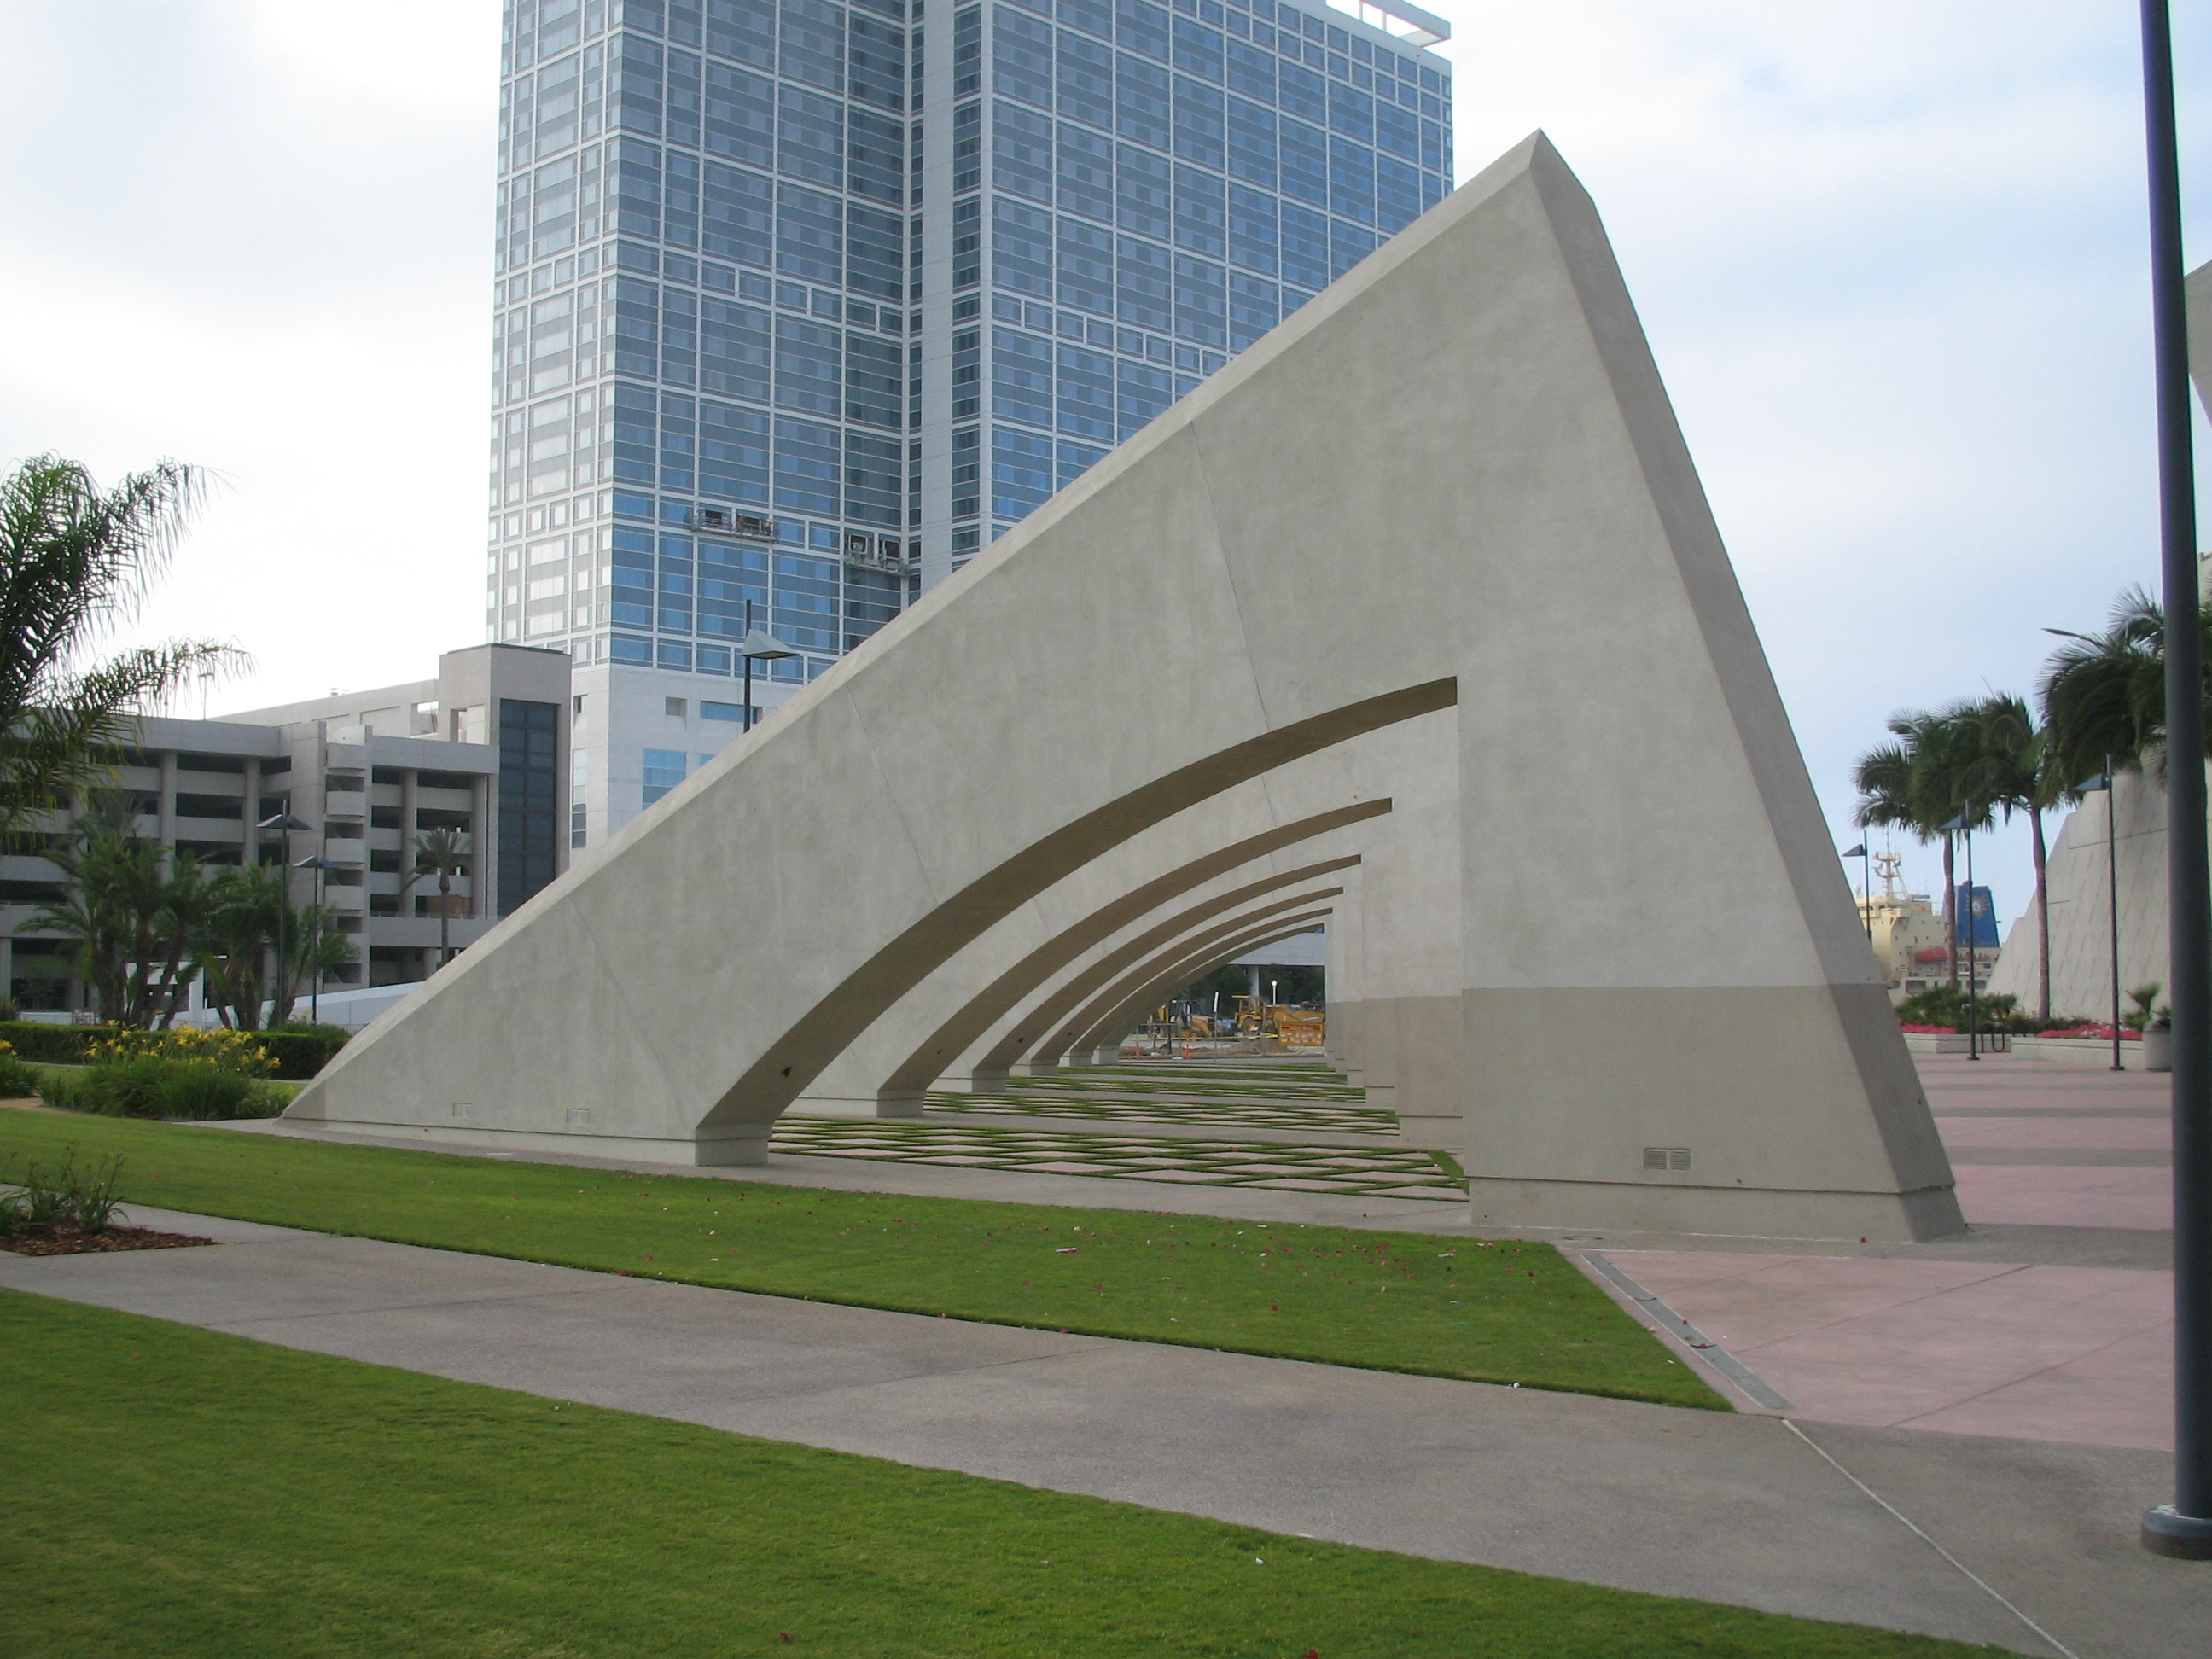
\includegraphics[width=0.95\textwidth]{triangle_shapes.jpg}
  \begin{center}
    {\large ``Triangle Shapes''}\par
    Foto di maxtodorov\par
    \url{http://www.flickr.com/photos/maxtodorov/3066505212/}\par
    Licenza: Creative Commons Attribution\par
  \end{center}
\newpage

\section{Definizioni relative ai triangoli}\label{sect:definizioni_triangoli}

Definiamo gli elementi principali di un triangolo
\begin{definizione}~
\begin{itemize*}
\item Un \emph{triangolo} è un poligono di tre lati.
\item Si chiamano \emph{vertici} gli estremi dei lati.
\item Un vertice si dice \emph{opposto a un lato} se non appartiene a quel lato.
\item Si chiamano \emph{angoli interni} del triangolo i tre angoli formati dai lati.
\item Un angolo interno si dice \emph{angolo compreso tra due lati} quando i lati dell'angolo contengono dei lati del triangolo.
\item Un angolo interno si dice \emph{angolo adiacente a un lato} del triangolo quando uno dei suoi lati contiene quel lato del triangolo.
\item Un angolo si dice \emph{angolo esterno} al triangolo se è un angolo adiacente a un angolo interno.
\item Si dice \emph{bisettrice} relativa a un vertice, il segmento di bisettrice dell'angolo al vertice che ha per estremi il vertice stesso e il punto in cui essa incontra il lato opposto.
\item Si dice \emph{mediana} relativa a un lato il segmento che ha per estremi il punto medio del lato e il vertice opposto a quel lato.
\item Si dice \emph{altezza} di un triangolo relativa a un suo lato il segmento di perpendicolare che ha per estremi il vertice opposto al lato e il punto di intersezione della perpendicolare con la retta contenente il lato. 
\item Si dice \emph{asse} di un triangolo, relativo a un suo lato, la perpendicolare al lato condotta nel suo punto medio.
\end{itemize*}
\end{definizione}

Nel triangolo (a) della figura seguente, $A$, $B$ e $C$ sono i vertici del triangolo, il vertice $A$ è opposto al lato $a$, l'angolo $\alpha$ è interno al triangolo ed è compreso tra i lati $AB$ e $AC$, mentre l'angolo $\beta$ è esterno. Nel triangolo (b) $AL$ è la bisettrice dell'angolo nel vertice $A$, $AH$ è altezza relativa alla base $BC$, $AM$ è la mediana relativa al lato $BC$ e la retta $r$ è l'asse di $BC$.

\begin{figure}[htb]
\centering% (c) 2014 Daniele Masini - d.masini.it@gmail.com
\begin{tikzpicture}[scale=1.5,font=\small]
\usetikzlibrary{calc}

\begin{scope}

\coordinate (b) at (0,0);
\coordinate (a) at (1.7,1.4);
\coordinate (c) at (2,0);

\draw[thick] (b) node[below] {$B$} -- node[below,midway] {$a$} (c) node[below] {$C$} -- (a) node[above] {$A$} -- cycle;
\draw[dotted] (c) -- ($(b)!1.35!(c)$) coordinate (d);

\begin{scope}
\clip (c) -- (d) -- (2.5,1) -- (a) -- cycle;
\draw[red] (c) circle (0.4);
\end{scope}
\node at ([shift={(11pt,12pt)}]c) {$\beta$};

\begin{scope}
\clip (b) -- (a) -- (c) -- cycle;
\draw[blue] (a) circle (0.4);
\end{scope}
\node at ([shift={(-5pt,-15pt)}]a) {$\alpha$};

\node at (1.2,-0.6) {(a)};

%\node at (2.5,1.2) {angolo};
%\node at (2.5,0.9) {esterno};
\end{scope}

\begin{scope}[xshift=4cm]

\coordinate (b) at (0,0);
\coordinate (a) at (1.7,1.4);
\coordinate (c) at (2,0);

\draw[thick] (b) node[below] {$B$} -- (c) node[below] {$C$} -- (a) node[above] {$A$} -- cycle;

%\begin{scope}
%\clip (b) -- (a) -- (c) -- cycle;
%\draw (a) node[left=3pt, below=15pt] {$\alpha$} circle (0.4);
%\end{scope}

\coordinate (m) at ($(b)!0.5!(c)$);

\draw[green!60!black,dashdotted] ($(m)!0.7cm!90:(c)$) coordinate (r) -- ($(m)!-.4cm!90:(c)$); % asse
\node at ([shift={(-3pt,-10pt)}]r) {$r$};
\draw[red,dashed] (m) node[black,below] {$M$} -- (a); % mediana
\draw[blue,dashed] (a) -- ($(b)!(a)!(c)$) node[black,below] {$H$}; % altezza

\node [circle] (circ1) at (a) [minimum size=2cm] {}; % circonferenza con centro in A
\coordinate (u) at (intersection of a--b and circ1);
\coordinate (v) at (intersection of a--c and circ1);
\node [circle] (circ2) at (u) [minimum size=2cm] {}; % circonferenza con centro in U
\node [circle] (circ3) at (v) [minimum size=2cm] {}; % circonferenza con centro in V
\coordinate (bis) at (intersection 1 of circ2 and circ3);
% la bisettrice di A passa per A e per bis1
\coordinate (bi) at ($(a)!5!(bis)$);
\coordinate (bt) at (intersection of b--c and a--bi);
\draw[orange!90!black,dashed] (a) -- (bt) node [black,below] {$L$}; % bisettrice


\node at (1,-0.6) {(b)};
\end{scope}

\end{tikzpicture}

%\caption{Triangolo. Vertici, angoli, bisettrice, mediana, asse.}\label{fig:triangolo1}
\end{figure}

I triangoli possono essere classificati rispetto ai lati
\begin{definizione}~
\begin{itemize*}
\item un triangolo si dice \emph{equilatero} se ha i tre lati congruenti;
\item un triangolo si dice \emph{isoscele} se ha (almeno) due lati congruenti;
\item un triangolo si dice \emph{scaleno} se ha i lati a due a due non congruenti.
\end{itemize*}
\end{definizione}

\begin{figure}[htb]
\centering% Copyright (c) 2015 Daniele Masini - d.masini.it@gmail.com

\begin{tikzpicture}[scale=1,font=\small]
\usetikzlibrary{calc}

\begin{scope}
\coordinate (b) at (0,0);
\coordinate (c) at (2,0);

\draw[thick] (b) node[below] {$B$} -- (c) node[below] {$C$} -- +(120:2) coordinate (a) node[above] {$A$} -- cycle;

\node at (1,-0.7) {triangolo equilatero};
\node at (1,-1.2) {$AB\cong AC\cong BC$};
\end{scope}

\begin{scope}[xshift=4.5cm]
\coordinate (b) at (0,0);
\coordinate (a) at (0.6,1.7);
\coordinate (c) at (1.2,0);

\draw[thick] (b) node[below] {$B$} -- (c) node[below] {$C$} -- (a) node[above] {$A$} -- cycle;

\node at (.6,-0.7) {triangolo isoscele};
\node at (.6,-1.2) {$AB\cong AC$};
\end{scope}


\begin{scope}[xshift=8cm]
\coordinate (b) at (0,0);
\coordinate (a) at (1.6,1.7);
\coordinate (c) at (2.5,0);

\draw[thick] (b) node[below] {$B$} -- (c) node[below] {$C$} -- (a) node[above] {$A$} -- cycle;

\node at (1.25,-0.7) {triangolo scaleno};
\node at (1.25,-1.2) {$AB\not\cong AC$, $AB\not\cong BC$, $AC\not\cong BC$};
\end{scope}

\end{tikzpicture}

\caption{Classificazione di un triangolo rispetto ai lati}\label{fig:class_triangolo_lati}
\end{figure}

\noindent o rispetto agli angoli
\begin{definizione}~
\begin{itemize*}
\item un triangolo si dice \emph{rettangolo} se ha un angolo interno retto; in un triangolo rettangolo si chiama \emph{ipotenusa} il lato che si oppone all'angolo retto e si chiamano \emph{cateti} i lati adiacenti all'angolo retto;
\item un triangolo si dice \emph{ottusangolo} se ha un angolo interno ottuso;
\item un triangolo si dice \emph{acutangolo} se ha tutti gli angoli interni acuti.
\end{itemize*}
\end{definizione}

\begin{figure}[htb]
\centering% (c) 2014 Daniele Masini - d.masini.it@gmail.com
\begin{tikzpicture}[scale=1,font=\small]
\usetikzlibrary{calc}

\begin{scope}
\coordinate (a) at (0,1.7);
\coordinate (b) at (0,0);
\coordinate (c) at (2.2,0);

\draw[thick] (b) node[below] {$B$} -- node[below,midway,sloped] {cateto} (c) node[below] {$C$} -- node[above,midway,sloped] {ipotenusa} (a) node[above] {$A$} -- cycle;
\path (b) -- node[above,midway,sloped] {cateto} (a);
\draw[red] ([shift={(10pt,0)}]b) -- ([shift={(10pt,10pt)}]b) -- ([shift={(0pt,10pt)}]b);

\node at (1.1,-0.8) {triangolo rettangolo};
\node at (1.1,-1.3) {$A\widehat{B}C=90\grado$};
\end{scope}

\begin{scope}[xshift=5cm]
\coordinate (b) at (0,0);
\coordinate (a) at (-0.7,1.7);
\coordinate (c) at (1.5,0);

\draw[thick] (b) node[below] {$B$} -- (c) node[below] {$C$} -- (a) node[above] {$A$} -- cycle;

\begin{scope}
\clip (a) -- (b) -- (c) -- (1.5,1.7) -- cycle;
\draw[red] (b) circle (0.4);
\end{scope}

\node at (.4,-0.8) {triangolo ottusangolo};
\node at (.4,-1.3) {$A\widehat{B}C>90\grado$};
\end{scope}

\begin{scope}[xshift=9cm]
\coordinate (b) at (0,0);
\coordinate (a) at (1.6,1.7);
\coordinate (c) at (2.5,0);

\draw[thick] (b) node[below] {$B$} -- (c) node[below] {$C$} -- (a) node[above] {$A$} -- cycle;

\begin{scope}
\clip (a) -- (b) -- (c) -- cycle;
\draw[blue] (b) circle (0.4);
\draw[blue] (a) circle (0.4);
\draw[blue] (c) circle (0.4);
\end{scope}

\node at (1.25,-0.8) {triangolo acutangolo};
\node at (1.25,-1.3) {$A\widehat{B}C<90\grado$, $B\widehat{C}A<90\grado$, $C\widehat{A}B<90\grado$};
\end{scope}

\end{tikzpicture}

\caption{Classificazione di un triangolo rispetto agli angoli}\label{fig:class_triangolo_angoli}
\end{figure}

\section{Primo e secondo criterio di congruenza dei triangoli}\label{sect:primo_secondo_criterio_di_congruenza_triangoli}

Ricordiamo che due figure piane si dicono \emph{congruenti} se sono sovrapponibili, cioè se è possibile spostare una sull'altra, senza deformarle, in modo che coincidano perfettamente. 

In particolare, due triangoli sono sovrapponibili se hanno ``ordinatamente'' congruenti i tre lati e i tre angoli. Con il termine ordinatamente intendiamo che, a partire da una coppia di vertici (il primo di un triangolo ed il secondo dell'altro) procedendo lungo il contorno in senso orario, oppure antiorario, incontriamo lati tra loro congruenti e vertici di angoli tra loro congruenti. Nel caso dei triangoli, questo succede esattamente quando angoli congruenti nei due triangoli sono compresi tra coppie di lati congruenti o, in maniera equivalente, quando sono opposti a lati congruenti.

I criteri di congruenza dei triangoli ci dicono che è sufficiente conoscere la congruenza di solo alcuni elementi dei due triangoli, generalmente tre elementi di un triangolo congruenti a tre elementi dell'altro triangolo, per poter affermare che i due triangoli sono tra loro congruenti, e quindi dedurne la congruenza degli altri elementi.

Un modo tradizionale di presentare l'argomento, dovuto allo stesso Euclide, è quello di ``dimostrare'' i primi due criteri di congruenza dei triangoli facendo uso della definizione stessa di congruenza come ``uguaglianza per sovrapposizione'', e di utilizzarli successivamente per la verifica di altre proprietà.

Secondo il matematico tedesco Hilbert, il primo criterio di congruenza è invece un assioma e il secondo criterio può essere dimostrato per assurdo attraverso il primo. 

Presenteremo questi argomenti basilari alla maniera di Euclide.

\begin{teorema}[1\textsuperscript{o} Criterio di congruenza dei triangoli]
Due triangoli sono congruenti se hanno congruenti due lati e l'angolo tra essi compreso.
\end{teorema}

% figura ()
\begin{figure}[htb]
\centering% Copyright (c) 2015 Daniele Masini - d.masini.it@gmail.com

\begin{tikzpicture}[scale=1,font=\small]
\usetikzlibrary{calc}

\begin{scope}
\coordinate (a) at (0,0);
\coordinate (c) at (1.6,1.7);
\coordinate (b) at (2.5,0);
\draw[fill=yellow!10] (a) -- (b) -- (c) -- cycle;

\begin{scope}
\clip (a) -- (b) -- (c) -- cycle;
\draw[thick,orange!40,fill] (c) circle (0.5);
\node at ([shift={(-0.1,-0.7)}]c) {$\gamma$};
\end{scope}

\draw[thick] (a) node[below] {$A$} -- (b) node[below] {$B$} -- (c) node[above] {$C$} -- cycle;
\draw[red,very thick] (a) -- (c);
\draw[blue,very thick] (b) -- (c);

\end{scope}

\begin{scope}[xshift=4cm]
\coordinate (a) at (0,0);
\coordinate (c) at (1.6,1.7);
\coordinate (b) at (2.5,0);
\draw[fill=gray!10] (a) -- (b) -- (c) -- cycle;

\begin{scope}
\clip (a) -- (b) -- (c) -- cycle;
\draw[thick,orange!40,fill] (c) circle (0.5);\node at ([shift={(-0.1,-0.7)}]c) {$\gamma'$};
\end{scope}

\draw[thick] (a) node[below] {$A'$} -- (b) node[below] {$B'$} -- (c) node[above] {$C'$} -- cycle;
\draw[red,very thick] (a) -- (c);
\draw[blue,very thick] (b) -- (c);

\end{scope}

\end{tikzpicture}

\end{figure}

\noindent Ipotesi: $AC\cong A'C'$, $BC\cong B'C'$, $\gamma \cong \gamma'$.\tab Tesi:  $ABC \cong A'B'C'$.

\begin{proof}
Vogliamo dimostrare che il triangolo $A’B’C’$ può essere portato a sovrapporsi perfettamente al triangolo $ABC$.
A tal proposito, portiamo il punto $C’$ sul punto $C$ in modo tale che la semiretta $C’A’$ sia sovrapposta alla semiretta $CA$ ed i punti $B$ e $B’$ siano nello stesso semipiano individuato dalla retta $AC$.
%Dopo questo movimento, i triangoli potrebbero trovarsi nella posizione della figura a lato?
Poiché per ipotesi i segmenti $AC$ e $A’C’$ sono congruenti, se $C$ coincide con $C’$ anche $A$ deve coincidere con $A’$.
%, mentre nella figura $A’C’$ è maggiore di $AC$. Né $A'$ può cadere all'interno di $AC$. In definitiva $C\equiv C'$ e $A\equiv A'$.

%Allora i triangoli potrebbero trovarsi almeno nella seguente posizione, nella quale $A$ e $A’$ coincidono?
%Tuttavia nemmeno questa posizione è possibile poiché
Avendo supposto per ipotesi che gli angoli $\gamma$ e $\gamma’$ sono congruenti, la semiretta per $CB$ e la semiretta per $C’B’$ devono sovrapporsi, in quanto devono formare lo stesso angolo con la semiretta per $CA$, ovvero per $C'A'$.

%A questo punto, rimane da fissare la posizione di $B’$ rispetto a $B$, cioè rimane da decidere se $B’$ cade internamente al segmento $CB$, come nella figura che segue, se $B’$ cade esternamente al segmento $CB$ o se $B’$ e $B$ coincidono.
Inoltre, poiché per ipotesi $BC\cong B'C'$, il punto $B’$ deve necessariamente coincidere con $B$.

Pertanto tutti i vertici del triangolo $A'B'C'$ si sovrappongono ai vertici del triangolo $ABC$ e di conseguenza i triangoli $ABC$ e $A’B’C’$ sono congruenti.
\end{proof}

\begin{teorema}[2\textsuperscript{o} Criterio di congruenza dei triangoli]
Due triangoli sono congruenti se hanno congruenti due angoli e il lato tra essi compreso.
\end{teorema}

\begin{figure}[htb]
\centering\begin{tikzpicture}[scale=1,font=\small]
\usetikzlibrary{calc}

\begin{scope}
\coordinate (a) at (0,0);
\coordinate (c) at (1.6,1.7);
\coordinate (b) at (2.5,0);
\draw[fill=yellow!10] (a) -- (b) -- (c) -- cycle;

\begin{scope}
\clip (a) -- (b) -- (c) -- cycle;
\draw[thick,red!50,fill] (a) circle (0.5);
\node at ([shift={(0.7,0.3)}]a) {$\alpha$};
\draw[thick,orange!50,fill] (b) circle (0.5);
\node at ([shift={(-0.7,0.3)}]b) {$\beta$};
\end{scope}

\draw[thick] (a) node[below] {$A$} -- (b) node[below] {$B$} -- (c) node[above] {$C$} -- cycle;
\draw[blue,very thick] (a) -- (b);


\end{scope}

\begin{scope}[xshift=4cm]
\coordinate (a) at (0,0);
\coordinate (c) at (1.6,1.7);
\coordinate (b) at (2.5,0);
\draw[fill=gray!10] (a) -- (b) -- (c) -- cycle;

\begin{scope}
\clip (a) -- (b) -- (c) -- cycle;
\draw[thick,red!50,fill] (a) circle (0.5);
\node at ([shift={(0.7,0.3)}]a) {$\alpha'$};
\draw[thick,orange!50,fill] (b) circle (0.5);
\node at ([shift={(-0.7,0.3)}]b) {$\beta'$};
\end{scope}

\draw[thick] (a) node[below] {$A'$} -- (b) node[below] {$B'$} -- (c) node[above] {$C'$} -- cycle;
\draw[blue,very thick] (a) -- (b);

\end{scope}

\end{tikzpicture}

\end{figure}

\noindent Ipotesi: $AB\cong A'B'$, $\alpha\cong \alpha'$, $\beta \cong \beta'$.\tab Tesi:  $ABC \cong A'B'C'$.

\begin{proof}
Vogliamo dimostrare che il triangolo $A'B'C'$ può essere portato a sovrapporsi perfettamente al triangolo $ABC$.
A tal proposito, in virtù della congruenza dei lati $AB$ e $A'B'$, portiamo a sovrapporre il segmento $A'B'$ al segmento $AB$ in maniera tale che $A'$ coincida con $A$, $B'$ coincida con $B$ e i punti $C$ e $C'$ siano nello stesso semipiano individuato dalla retta $AB$. 

%I due triangoli potrebbero trovarsi nella posizione rappresentata a fianco?
Dalla congruenza degli angoli $\alpha$ e $\alpha'$ segue che la semiretta $A'C'$ sarà sovrapposta alla semiretta $AC$; analogamente, dalla congruenza degli angoli $\beta$ e $\beta'$ segue che la semiretta $B'C'$ sarà sovrapposta alla semiretta $BC$. Dunque $C$ e $C'$ devono necessariamente coincidere, perché sono l'unica intersezione di due rette incidenti.

Poiché, dunque, i tre vertici si sono sovrapposti, i due triangoli sono completamente sovrapposti e quindi sono congruenti.
\end{proof}

\begin{exrig}
\begin{esempio}\label{esempio:2.1}
Si considerino due rette incidenti, $r$ ed $s$, ed il loro punto in comune $P$. Sulle semirette opposte di origine $P$ si prendano punti equidistanti da $P$, come in figura, in maniera tale che $AP\cong PB$, $CP\cong PD$. Dimostra che, unendo i quattro punti in modo da costruire un quadrilatero, i quattro triangoli che si vengono a formare sono a due a due congruenti: $ACP\cong BDP$, $ADP\cong BPC$.

Realizziamo il disegno (figura~\ref{fig:esempio2.1}) ed esplicitiamo ipotesi e tesi.

\begin{figure}[htb]
\centering% (c) 2014 Daniele Masini - d.masini.it@gmail.com
\begin{tikzpicture}[scale=1,font=\small]
\usetikzlibrary{calc}

\begin{scope}
\coordinate (s1) at (-3,-0.7);
\coordinate (s2) at (3,0.7);
\coordinate (r1) at (-3,1.5);
\coordinate (r2) at (3,-1.5);

\coordinate (p) at (intersection of r1--r2 and s1--s2);
\coordinate (a) at ($(p)!2.5cm!(r1)$);
\coordinate (b) at ($(p)!2.5cm!(r2)$);
\coordinate (c) at ($(p)!1.7cm!(s1)$);
\coordinate (d) at ($(p)!1.7cm!(s2)$);
\draw[fill] (a) circle (1.5pt) node[above] {$A$};
\draw[fill] (b) circle (1.5pt) node[below] {$B$};
\draw[fill] (c) circle (1.5pt) node[below] {$C$};
\draw[fill] (d) circle (1.5pt) node[above] {$D$};
\draw (a) -- (c) -- (b) -- (d) -- cycle;

\begin{scope}
\clip (a) -- (p) -- (c) -- cycle;
\draw[red!90] (p) circle (0.5);
%\node at ([shift={(0.7,0.3)}]p) {$\alpha$};
\end{scope}

\begin{scope}
\clip (b) -- (p) -- (d) -- cycle;
\draw[red!90] (p) circle (0.5);
%\node at ([shift={(0.7,0.3)}]p) {$\alpha$};
\end{scope}
\draw (s1) node[above] {$s$} -- (s2);
\draw (r1) node[above] {$r$} -- (r2);
\draw[fill] (p) circle (1.5pt) node[above] {$P$};

\end{scope}


\end{tikzpicture}

\caption{Esempio~\ref{esempio:2.1}}\label{fig:esempio2.1}
\end{figure}

\noindent Ipotesi: $r\cap s=P$, $AP\cong PB$, $CP\cong PD$.\tab\tab Tesi: $ACP\cong BDP$, $ADP\cong BPC$.

\begin{proof}
I triangoli $ACP$ e $BPD$ hanno: $AP\cong PB$ per ipotesi, $CP\cong PD$ per ipotesi, $A\widehat{P}C\cong B\widehat{P}D$ perché opposti al vertice. Pertanto sono congruenti per il 1\textsuperscript{o} criterio di congruenza dei triangoli.

Analogamente, i triangoli $ADP$ e $BPC$ hanno: \ldots\ldots\ldots\ldots\ldots\ldots\ldots
\end{proof}
\end{esempio}

\begin{esempio}\label{esempio:2.2}
Si considerino un segmento $AB$ ed il suo punto medio $M$. Si tracci una generica retta $r$ passante per $M$ e distinta dalla retta per $AB$. Si traccino inoltre due semirette di origine rispettivamente $A$ e $B$, situate nei due semipiani opposti rispetto alla retta per $AB$, che intersechino la retta $r$ rispettivamente in $C$ e in $D$ e che formino con la retta per $AB$ due angoli congruenti (vedi figura~\ref{fig:esempio2.2}). Detti $C$ e $D$ i rispettivi punti di intersezione delle due semirette con la retta $r$, dimostra che i triangoli $AMC$ e $BMD$ sono congruenti.

\begin{figure}[htb]
\centering% Copyright (c) 2015 Daniele Masini - d.masini.it@gmail.com

\begin{tikzpicture}[scale=1,font=\small]
\usetikzlibrary{calc}

\begin{scope}
\coordinate (a) at (-3,0);
\coordinate (b) at (3,0);
\coordinate (m) at (0,0);
\coordinate (r1) at (-1.7,-2);
\coordinate (r2) at (1.7,2);
\coordinate (s1) at ([shift={(135:3)}]b);
\coordinate (t1) at ([shift={(-45:3)}]a);
\coordinate (c) at (intersection of r1--r2 and a--t1);
\coordinate (d) at (intersection of r1--r2 and b--s1);

\begin{scope}
\clip (a) -- (m) -- (c) -- cycle;
\draw[fill,orange!40] (a) circle (0.5);
\draw[red!90] (m) circle (0.5);
%\node at ([shift={(0.7,0.3)}]p) {$\alpha$};
\end{scope}

\begin{scope}
\clip (b) -- (m) -- (d) -- cycle;
\draw[fill,orange!40] (b) circle (0.5);
\draw[red!90] (m) circle (0.5);
%\node at ([shift={(0.7,0.3)}]p) {$\alpha$};
\end{scope}

\draw[fill] (a) circle (1.5pt) node[above] {$A$};
\draw[fill] (b) circle (1.5pt) node[below] {$B$};
\draw[fill] (c) circle (1.5pt) node[right] {$C$};
\draw[fill] (d) circle (1.5pt) node[left] {$D$};
\draw (a) -- (b);
\draw (r1) -- (r2);
\draw (a) -- (t1);
\draw (b) -- (s1);

\draw (r1) node[left] {$r$} -- (r2);
\draw[fill] (m) circle (1.5pt) node[left = 3pt, above=0pt] {$M$};

\end{scope}


\end{tikzpicture}

\caption{Esempio~\ref{esempio:2.2}}\label{fig:esempio2.2}
\end{figure}

\noindent Ipotesi: $AM\cong MB$, $M\widehat{A}C\cong M\widehat{B}D$.\tab Tesi: $AMC\cong BMD$.

\begin{proof}
I segmenti $AM$ e $MB$ sono congruenti in quanto $M$ è il punto medio di $AB$, gli angoli di vertice $M$ sono congruenti perché opposti al vertice, gli angoli di vertici $A$ e $B$ sono congruenti per costruzione. Allora i triangoli $AMC$ e $BMD$ sono congruenti per il 2\textsuperscript{o} criterio di congruenza dei triangoli.
\end{proof}
\end{esempio}
\end{exrig}

\section{Teoremi del triangolo isoscele}\label{sect:teoremi_triangolo_isoscele}

Il \emph{triangolo isoscele} ha almeno due lati congruenti, l'eventuale lato non congruente si chiama \emph{base}, i due lati congruenti si dicono \emph{lati obliqui}.

Il \emph{triangolo equilatero} è un caso particolare di triangolo isoscele: si dice che \emph{il triangolo equilatero è isoscele rispetto a qualsiasi lato preso come base}.

\begin{teorema}[del triangolo isoscele {[}teorema diretto{]}]
In un triangolo isoscele gli angoli alla base sono congruenti.
\end{teorema}

\begin{figure}[htb]
\centering% Copyright (c) 2015 Daniele Masini - d.masini.it@gmail.com

\begin{tikzpicture}[scale=0.9,font=\small]
\usetikzlibrary{calc}

\begin{scope}
\coordinate (a) at (-1.3,0);
\coordinate (b) at (1.3,0);
\coordinate (c) at (0,3);
\coordinate (k) at (0,0);

\begin{scope}
\clip (a) -- (b) -- (c) -- cycle;
\draw[orange] (a) circle (0.5);
\draw[orange] (b) circle (0.5);
\node at ([shift={(0.6,0.4)}]a) {$\alpha$};
\node at ([shift={(-0.6,0.4)}]b) {$\beta$};
\end{scope}

\begin{scope}
\clip (a) -- (c) -- (k) -- cycle;
\draw[red] (c) circle (0.65);
\end{scope}

\begin{scope}
\clip (b) -- (c) -- (k) -- cycle;
\draw[blue] (c) circle (0.65);
\end{scope}


\draw[thick] (a) node[below] {$A$} -- (b) node[below] {$B$} -- (c) node[above] {$C$} -- cycle;
\draw[dashed] (c) -- (k);
\node[below] at (k) {$K$};

\end{scope}


\end{tikzpicture}

\end{figure}

\noindent Ipotesi: $AC\cong BC$.\tab Tesi: $\alpha\cong \beta$.

\begin{proof}
Tracciamo la bisettrice $CK$ dell'angolo in $C$.
I triangoli $ACK$ e $BCK$ sono congruenti per il primo criterio, infatti hanno:
\begin{itemize*}
\item $AC\cong CB$ per ipotesi;
\item $CK$ lato in comune;
\item $A\widehat{C}K\cong B\widehat{C}K$ perché $CK$ è la bisettrice dell'angolo in $C$.
\end{itemize*}
Pertanto, essendo congruenti, i due triangoli hanno tutti gli elementi congruenti, in particolare l'angolo $\alpha$ (in $A$) è congruente all'angolo $\beta$ (in $B$).
\end{proof}

Il teorema precedente è invertibile, nel senso che è valido anche il teorema inverso, quello che si ottiene scambiando tra loro ipotesi e tesi.

\begin{teorema}[del triangolo isoscele {[}teorema inverso{]}]
Se un triangolo ha due angoli congruenti, allora è isoscele (rispetto al lato compreso tra gli angoli congruenti preso come base).
\end{teorema}

\begin{figure}[htb]
\centering\begin{tikzpicture}[scale=0.9,font=\small]
\usetikzlibrary{calc}

\begin{scope}
\coordinate (a) at (-1.3,0);
\coordinate (b) at (1.3,0);
\coordinate (c) at (0,3);

\begin{scope}
\clip (a) -- (b) -- (c) -- cycle;
\draw[fill,orange!40] (a) circle (0.5);
\draw[fill,orange!40] (b) circle (0.5);
\node at ([shift={(0.6,0.4)}]a) {$\alpha$};
\node at ([shift={(-0.6,0.4)}]b) {$\beta$};
\end{scope}

\draw[thick] (a) node[left] {$A$} -- (b) node[right] {$B$} -- (c) node[above] {$C$} -- cycle;

\draw (a) -- ($(a)!-1.5cm!(c)$) node[below] {$D$} -- (b);
\draw (b) -- ($(b)!-1.5cm!(c)$) node[below] {$E$} -- (a);

\end{scope}


\end{tikzpicture}

\end{figure}

\noindent Ipotesi: $\alpha\cong \beta$.\tab Tesi: $AC\cong BC$.

\begin{proof}
Procediamo per passi, realizzando una costruzione che ci permetta di confrontare coppie di triangoli congruenti. Prolunghiamo i lati $AC$ e $BC$ dalla parte di $A$ e di $B$ rispettivamente, e sui prolungamenti prendiamo due punti $D$ ed $E$ in maniera tale che risulti $AD\cong BE$.

Osserviamo che i triangoli $ADB$ e $BAE$ risultano congruenti per il 1\textsuperscript{o} criterio, avendo in comune il lato $AB$ ed essendo $AD\cong BE$ per costruzione e $D\widehat{A}B\cong A\widehat{B}E$ perché adiacenti agli angoli $C\widehat{A}B$ e $C\widehat{B}A$ congruenti per ipotesi. Pertanto, tutti gli elementi dei due triangoli $ADB$ e $AEB$ sono ordinatamente congruenti, in particolare $DB\cong AE$, $A\widehat{D}B\cong B\widehat{E}A$ e $A\widehat{B}D\cong B\widehat{A}E$.

I triangoli $CDB$ e $CAE$ risultano dunque congruenti per il 2\textsuperscript{o} criterio poiché hanno $DB\cong AE$, $C\widehat{D}B\cong C\widehat{E}A$ per quanto appena dimostrato e $C\widehat{D}B\cong C\widehat{A}E$ perché somma di angoli rispettivamente congruenti: $C\widehat{B}D\cong C\widehat{B}A + A\widehat{B}D$ e $C\widehat{A}E\cong C\widehat{A}B + B\widehat{A}E$.

Pertanto, i restanti elementi dei due triangoli risultano ordinatamente congruenti, in particolare $CB\cong CA$, che è la tesi che volevamo dimostrare.
\end{proof}


Dai due teoremi precedenti seguono importanti proprietà, che qui riportiamo come corollari.

\begin{corollario}
Un triangolo equilatero è anche equiangolo.
\end{corollario}

\begin{proof}
Poiché un triangolo equilatero è isoscele rispetto a qualsiasi lato preso come base, la tesi segue dal teorema diretto del triangolo isoscele.
\end{proof}

\begin{corollario}
Se un triangolo è equiangolo allora è equilatero.
\end{corollario}

\begin{proof}
Possiamo confrontare gli angoli a due a due; risulteranno i lati congruenti a due a due in base al teorema inverso del triangolo isoscele.
\end{proof}

\begin{corollario}
Un triangolo scaleno non ha angoli congruenti.
\end{corollario}

\begin{proof}
Se per assurdo un triangolo scaleno avesse due angoli congruenti, allora risulterebbe isoscele, in base al teorema inverso del triangolo isoscele.
\end{proof}

\begin{corollario}
Se un triangolo non ha angoli congruenti allora è scaleno.
\end{corollario}

\begin{proof}
Se un triangolo non ha angoli tra loro congruenti non può essere isoscele.
\end{proof}

\begin{proposizione}[Proprietà del triangolo isoscele]
In ogni triangolo isoscele, la mediana relativa alla base è anche altezza e bisettrice.
\end{proposizione}
Nella figura, $CJ$ è per ipotesi la bisettrice dell'angolo al vertice $\gamma$ del triangolo $ABC$, $FK$ è la mediana relativa alla base $DE$ del triangolo $DEF$, $IL$ è l'altezza relativa alla base $GH$ del triangolo $GHI$.

\begin{figure}[htb]
\centering% (c) 2014 Daniele Masini - d.masini.it@gmail.com
\begin{tikzpicture}[scale=0.9,font=\small]
\usetikzlibrary{calc}

\begin{scope}
\coordinate (a) at (-1.3,0);
\coordinate (b) at (1.3,0);
\coordinate (c) at (0,3);
\coordinate (j) at (0,0);

\begin{scope}
\clip (a) -- (b) -- (c) -- cycle;
\draw[fill,orange!40] (a) circle (0.5);
\draw[fill,orange!40] (b) circle (0.5);
\draw[fill,red!30] (c) circle (0.6);
\node at ([shift={(0.6,0.4)}]a) {$\alpha_1$};
\node at ([shift={(-0.6,0.4)}]b) {$\beta_1$};
\node at ([shift={(0,-0.9)}]c) {$\gamma_1$};
\end{scope}

\begin{scope}
\clip (a) -- (c) -- (j) -- cycle;
\draw[thick,red] (c) circle (0.6);
\end{scope}

\begin{scope}
\clip (b) -- (c) -- (j) -- cycle;
\draw[thick,blue] (c) circle (0.6);
\end{scope}

\draw[dashed] (c) -- (j) node[below] {$J$};
\draw[thick] (a) node[below] {$A$} -- (b) node[below] {$B$} -- (c) node[above] {$C$} -- cycle;

\end{scope}


\begin{scope}[xshift=4cm]
\coordinate (a) at (-1.3,0);
\coordinate (b) at (1.3,0);
\coordinate (c) at (0,3);
\coordinate (j) at (0,0);

\begin{scope}
\clip (a) -- (b) -- (c) -- cycle;
\draw[fill,orange!40] (a) circle (0.5);
\draw[fill,orange!40] (b) circle (0.5);
\node at ([shift={(0.6,0.4)}]a) {$\alpha_2$};
\node at ([shift={(-0.6,0.4)}]b) {$\beta_2$};
\end{scope}

\draw[dashed] (c) -- (j) node[below] {$K$};
\draw[thick] (a) node[below] {$D$} -- (b) node[below] {$E$} -- (c) node[above] {$F$} -- cycle;

\end{scope}

\begin{scope}[xshift=8cm]
\coordinate (a) at (-1.3,0);
\coordinate (b) at (1.3,0);
\coordinate (c) at (0,3);
\coordinate (j) at (0,0);

\begin{scope}
\clip (a) -- (b) -- (c) -- cycle;
\draw[fill,orange!40] (a) circle (0.5);
\draw[fill,orange!40] (b) circle (0.5);
\node at ([shift={(0.6,0.4)}]a) {$\alpha_3$};
\node at ([shift={(-0.6,0.4)}]b) {$\beta_3$};
\end{scope}

\begin{scope}
\clip (a) -- (b) -- (c) -- cycle;
\draw[fill,blue!30] (j) circle (0.4);
\end{scope}

\draw[dashed] (c) -- (j) node[below] {$L$};
\draw[thick] (a) node[below] {$G$} -- (b) node[below] {$H$} -- (c) node[above] {$I$} -- cycle;

\end{scope}

\end{tikzpicture}

\end{figure}

Dividiamo l'enunciato in tre parti:
\begin{enumeratea}
\item In un triangolo isoscele la bisettrice dell'angolo al vertice è anche altezza e mediana relativa alla base.
\item In un triangolo isoscele la mediana relativa alla base è anche bisettrice dell'angolo al vertice e altezza relativa alla base.
\item In un triangolo isoscele l'altezza relativa alla base è anche bisettrice dell'angolo al vertice e mediana relativa alla base.
\end{enumeratea}

Per ciascuna di esse scriviamo ipotesi e tesi.
\begin{enumeratea}
\item In $ABC$:	Ipotesi: $AC\cong CB$, $\alpha_1\cong \beta_1$, $A\widehat{C}J\cong B\widehat{C}J$. Tesi: $CJ\perp AB$, $AJ\perp JB$.
\item In $DEF$:	\,Ipotesi: $DF\cong FE$, $\alpha_2\cong \beta_2$, $DK\cong KE$.\tab Tesi: $FK\perp DE$, $D\widehat{F}K\cong E\widehat{F}K$.
\item In $GHI$:	\,Ipotesi: $IG\cong IH$, $\alpha_3\cong \beta_3$, $IL\cong GH$.\tab Tesi: $GL\perp LH$, $G\widehat{I}L\cong H\widehat{I}L$.
\end{enumeratea}

\begin{proof}
Avviamo la dimostrazione delle prime due parti, che lasciamo completare al lettore e rimandiamo al prossimo capitolo la dimostrazione della terza.

\begin{enumeratea}
\item I triangoli $AJC$ e $CJB$ sono congruenti per il 2\textsuperscript{o} criterio. Infatti hanno \ldots\ldots\ldots\ldots{}\\
Dunque $AJ\cong JB$ e $A\widehat{J}C\cong C\widehat{J}B$ che risultano pertanto retti in quanto adiacenti.  
\item I triangoli $DKF$ e $FKE$ sono congruenti per il 1\textsuperscript{o} criterio. Infatti hanno \ldots\ldots\ldots\ldots{}\\
Dunque $D\widehat{F}K\cong E\widehat{F}K$ e $F\widehat{K}D\cong F\widehat{K}E$ che risultano pertanto retti in quanto adiacenti.
\end{enumeratea}
\end{proof}

\section{Terzo criterio di congruenza dei triangoli}\label{sect:terzo_criterio_congruenza_triangoli}

\begin{teorema}[3\textsuperscript{o} criterio di congruenza dei triangoli]
Due triangoli sono congruenti se hanno congruenti le tre coppie di lati.
\end{teorema}

\begin{figure}[htb]
\centering% (c) 2014 Daniele Masini - d.masini.it@gmail.com
\begin{tikzpicture}[scale=1,font=\small]
\usetikzlibrary{calc}

\begin{scope}
\coordinate (a) at (0,0);
\coordinate (c) at (1.6,1.7);
\coordinate (b) at (2.5,0);

\draw[fill=yellow!10] (a) -- (b) -- (c) -- cycle;
\draw[thick] (a) node[left] {$A$} -- (b) node[right] {$B$} -- (c) node[above] {$C$} -- cycle;
\draw[blue,very thick] (a) -- (c);
\draw[red,very thick] (c) -- (b);
\draw[green!60!black,very thick] (a) -- (b);

\end{scope}

\begin{scope}[xshift=5cm]
\coordinate (a) at (0,0);
\coordinate (c) at (1.6,1.7);
\coordinate (b) at (2.5,0);

\draw[fill=gray!10] (a) node[left] {$A'$} -- (b) node[right] {$B'$} -- (c) node[above] {$C'$} -- cycle;
\draw[blue,very thick] (a) -- (c);
\draw[red,very thick] (c) -- (b);
\draw[green!60!black,very thick] (a) -- (b);

\end{scope}

\end{tikzpicture}

\end{figure}

\noindent Ipotesi: $AB\cong A'B'$, $BC\cong B'C'$, $AC\cong A'C'$.\tab Tesi: $ABC\cong A'B'C'$.

\begin{figure}[htb]
\centering% Copyright (c) 2015 Daniele Masini - d.masini.it@gmail.com

\begin{tikzpicture}[scale=.7,font=\small]
\usetikzlibrary{calc}

\begin{scope}
\coordinate (a) at (0,0);
\coordinate (c) at (1.6,1.7);
\coordinate (b) at (2.5,0);
\coordinate (c1) at (1.6,-1.7);

\draw[fill=gray!10] (a) -- (b) -- (c1) -- cycle;

\draw[fill=yellow!10] (a) -- (b) -- (c) -- cycle;
\draw (a) node[left] {$A\equiv A'$} -- (b) node[right] {$B\equiv B'$} -- (c) node[above] {$C$} -- cycle;
\draw[blue,very thick] (a) -- (c);
\draw[red,very thick] (c) -- (b);
\draw[green!60!black,very thick] (a) -- (b);

\draw[very thick,blue] (a) -- (c1);
\draw[very thick,red] (b) -- (c1);
\draw[dashed] (c) -- (c1) node[below] {$C'$};
\coordinate (d) at (intersection of a--b and c--c1);
\node[left=5pt, below] at (d) {$D$};

\node at (1.25,-2.9) {Caso 1};

\end{scope}


\begin{scope}[xshift=7.5cm]
\coordinate (a) at (0,0);
\coordinate (c) at (0,1.7);
\coordinate (b) at (2.5,0);
\coordinate (c1) at (0,-1.7);

\draw[fill=gray!10] (a) -- (b) -- (c1) -- cycle;

\draw[fill=yellow!10] (a) -- (b) -- (c) -- cycle;
\draw (a) node[left] {$A\equiv A'\equiv D$} -- (b) node[right] {$B\equiv B'$} -- (c) node[above] {$C$} -- cycle;
\draw[blue,very thick] (a) -- (c);
\draw[red,very thick] (c) -- (b);
\draw[green!60!black,very thick] (a) -- (b);

\draw[very thick,blue] (a) -- (c1);
\draw[very thick,red] (b) -- (c1) node[black,below] {$C'$};
\coordinate (d) at (intersection of a--b and c--c1);

\node at (1.25,-2.9) {Caso 2};

\end{scope}


\begin{scope}[xshift=14cm]
\coordinate (a) at (0,0);
\coordinate (c) at (-1,1.7);
\coordinate (b) at (2.5,0);
\coordinate (c1) at (-1,-1.7);

\draw[fill=gray!10] (a) -- (b) -- (c1) -- cycle;

\draw[fill=yellow!10] (a) -- (b) -- (c) -- cycle;
\draw (a) node[left=-1pt,above] {$A\equiv A'$} -- (b) node[right] {$B\equiv B'$} -- (c) node[above] {$C$} -- cycle;
\draw[blue,very thick] (a) -- (c);
\draw[red,very thick] (c) -- (b);
\draw[green!60!black,very thick] (a) -- (b);

\draw[very thick,blue] (a) -- (c1);
\draw[very thick,red] (b) -- (c1);
\draw[dashed] (c) -- (c1) node[below] {$C'$};
\coordinate (d) at (intersection of a--b and c--c1);
\draw[dashed] (a) -- (d);
%\node[left=5pt, below] at (d) {$D$};
\node[left] at (d) {$D$};

\node at (1,-2.9) {Caso 3};

\end{scope}

\end{tikzpicture}

\end{figure}

\begin{proof}
Abbiamo due triangoli, $ABC$ e $A'B'C'$, dei quali sappiamo che i lati dell'uno sono congruenti a quelli dell'altro. Ribaltiamo il triangolo $A'B'C'$ e portiamo il segmento $A'B'$ sul segmento $AB$ in modo che il punto $A'$ coincida con $A$, il punto $B'$ coincida con $B$ (ciò è possibile in quanto $AB\cong A'B'$) ed in modo che il punto $C'$ cada nel semipiano individuato dalla retta $AB$ opposto a quello in cui si trova $C$. Uniamo $C$ con $C'$. Viene fuori un disegno diverso a seconda che il punto di intersezione, che chiamiamo $D$, tra il segmento $CC'$ e la retta per $AB$, sia interno o esterno al segmento $AB$ oppure coincida con uno degli estremi ($A$ o $B$). Il punto $D$ esiste in ogni caso in quanto $C$ e $C'$ sono nei due semipiani opposti individuati dalla retta $AB$, pertanto il segmento $CC'$ deve necessariamente tagliare la retta per $AB$.

Caso 1: $D$ è interno ad $AB$.
Essendo $AC\cong A'C'$ e $CB\cong C'B'$, i triangoli $ACC'$ e $CC'B$ sono isosceli, entrambi sulla base $CC'$. Dunque, per il teorema (diretto) del triangolo isoscele, gli angoli alla base sono congruenti. Precisamente risulta: $A\widehat{C}C'\cong A\widehat{C'}C$ e $C'\widehat{C}B\cong C\widehat{C'}B$. Inoltre, $A\widehat{C}B\cong A\widehat{C'}B$ in quanto somme di angoli congruenti:
$A\widehat{C}B\cong A\widehat{C}D+D\widehat{C}B\cong A\widehat{C'}D+D\widehat{C'}B\cong A\widehat{C'}B$.
In conclusione $ABC$ e $ABC'$ sono congruenti per il primo criterio perché hanno: $AC\cong AC'$, $BC\cong BC'$, $A\widehat{C}B\cong A\widehat{C'}B$. 
Infine, poiché $ABC\cong ABC'$ e $ABC'\cong A'B'C'$ se ne deduce che $ABC\cong A'B'C'$.

Caso 2: $D$ coincide con uno dei due estremi (es.~$A$ e $A'$). 
Poiché per ipotesi $CB\cong C'B'$, il triangolo $CBC'$ è isoscele sulla base $CC'$, pertanto $A\widehat{C}B\cong A\widehat{C'}B$ in quanto angoli alla base di un triangolo isoscele. I triangoli $ABC$ e $ABC'$ sono quindi congruenti per il primo criterio perché hanno $AC\cong AC'$, $BC\cong BC'$ e $A\widehat{C}B\cong A\widehat{C'}B$. Infine, come per il caso precedente, poiché $ABC$ è congruente ad $ABC'$ e quest'ultimo è congruente ad $A'B'C'$ anche $ABC$ è congruente a $A'B'C'$.

Caso 3: $D$ cade esternamente al segmento $AB$.
Come nel caso 1, i triangoli $CAC'$ e $CBC'$ sono isosceli sulla base $CC'$, pertanto $A\widehat{C}C'\cong A\widehat{C'}C$ e $B\widehat{C}C'\cong B\widehat{C'}C$. Per differenza di angoli congruenti si ottiene che $A\widehat{C}B\cong A\widehat{C'}B$.
Infatti $A\widehat{C}B\cong D\widehat{C}B-D\widehat{C}A\cong D\widehat{C'}B-D\widehat{C'}A\cong A\widehat{C'}B$. Da ciò segue che i triangoli $ABC$ e $ABC'$ sono congruenti per il primo criterio in quanto hanno rispettivamente congruenti due lati e l'angolo tra essi compreso. Come per i casi precedenti, se $ABC$ è congruente a $ABC'$ è congruente anche a $A'B'C'$.
\end{proof}

\section{Congruenza dei poligoni}\label{sect:congruenza_poligoni}

Ricordiamo che due poligoni sono \emph{congruenti} se hanno lo stesso numero di lati ed hanno ``ordinatamente'' congruenti tutti i lati e tutti gli angoli corrispondenti.

Il seguente criterio di congruenza dei quadrilateri è una semplice applicazione del primo criterio di congruenza dei triangoli.
\begin{teorema}[1\textsuperscript{o} criterio di congruenza dei quadrilateri]
Due quadrilateri, aventi ordinatamente congruenti tre lati ed i due angoli tra essi compresi, sono congruenti.
\end{teorema}
Di conseguenza hanno ordinatamente congruenti anche il rimanente lato ed i rimanenti due angoli.

Conseguenza diretta del primo e del secondo criterio di congruenza dei triangoli è il seguente criterio.
\begin{teorema}[2\textsuperscript{o} criterio di congruenza dei quadrilateri]
Due quadrilateri, aventi ordinatamente congruenti due lati consecutivi e tre angoli (adiacenti ai due lati congruenti), sono congruenti.
\end{teorema}
Di conseguenza hanno ordinatamente congruenti anche il rimanente angolo ed i rimanenti due lati.

Conseguenza del primo e del terzo criterio di congruenza dei triangoli è il seguente criterio.
\begin{teorema}[3\textsuperscript{o} criterio di congruenza dei quadrilateri]
Due quadrilateri sono congruenti se hanno ordinatamente congruenti i quattro lati ed un angolo corrispondente.
\end{teorema}
Di conseguenza hanno ordinatamente congruenti anche i rimanenti tre angoli.

\begin{teorema}[Criteri di congruenza dei poligoni]
Due poligoni sono congruenti se hanno ordinatamente congruenti tutti i lati e tutti gli angoli compresi, tranne uno dei seguenti elementi su cui non si fa alcuna ipotesi:
\begin{itemize*}
\item due angoli consecutivi ed il lato compreso;
\item due lati consecutivi e l'angolo compreso;
\item tre angoli consecutivi.
\end{itemize*}
\end{teorema}

La dimostrazione di questi criteri è lasciata al lettore che potrà esercitarsi applicando i tre criteri di congruenza dei triangoli.


\newpage

% (c) 2014 Daniele Masini - d.masini.it@gmail.com
\section{Esercizi}

\begin{esercizio}
\label{ese:2.1}
In base alla figura rispondi alle seguenti domande 
\begin{enumeratea}
\item Il lato $AB$ si oppone all'angolo \ldots\ldots\ldots
\item L'angolo $\alpha$ si oppone al lato \ldots\ldots\ldots
\item L'angolo di vertice $C$ si chiama \ldots\ldots\ldots
\item L'angolo $\gamma$ è adiacente ai lati \ldots\ldots{} e \ldots\ldots
\item I lati $AB$ e $BC$ sono adiacenti all'angolo \ldots\ldots
\item I lati $AC$ e $AB$ formano l'angolo \ldots\ldots
\item Traccia l'angolo esterno al triangolo nel vertice $A$
\item Traccia la bisettrice dell'angolo $\beta$
\item Traccia l'altezza relativa alla base $AB$
\item Traccia la mediana relativa al lato $BC$
\end{enumeratea}
\end{esercizio}

% figura

\begin{esercizio}
\label{ese:2.2}
Disegna un segmento $AB$, quindi disegna i triangoli $ABC$ e $ABD$ che hanno la base $AB$ in comune.
\end{esercizio}

\begin{esercizio}
\label{ese:2.3}
Disegna le tre altezze di ciascuno dei seguenti triangoli.
\end{esercizio}

% figura

\begin{esercizio}
\label{ese:2.4}
Per ciascuna delle seguenti coppie di triangoli indica se sono congruenti ed eventualmente per quale criterio.
\end{esercizio}

Si sa che sono congruenti i lati $AB$ con $A'B'$ e $AC$ con $A'C'$, l'angolo $\widehat{A}$ con l'angolo $\widehat{A'}$.
I triangoli sono congruenti? 		SI	NO

Se sì, per il \ldots\ldots\ldots\ldots\ldots\ldots\ldots\ldots


Si sa che sono congruenti i lati $AB$ con $A'B'$ e gli angoli $\widehat{A}$ con $\widehat{B'}$ e $\widehat{B}$ con $\widehat{A'}$.
I triangoli sono congruenti? 		SI	NO

Se sì, per il \ldots\ldots\ldots\ldots\ldots\ldots\ldots\ldots


Si sa che sono congruenti i lati $AB$ con $A'B'$ e $BC$ con $A'C'$, l'angolo $\widehat{A}$ con $\widehat{A'}$.
I due triangoli sono congruenti? 	SI	NO

Se sì, per il \ldots\ldots\ldots\ldots\ldots\ldots\ldots\ldots

% figura

\begin{multicols}{2}

\subsubsection*{Dimostra le seguenti affermazioni, utilizzando il 1\textsuperscript{o} e il 2\textsuperscript{o} criterio di congruenza dei triangoli.}

\begin{esercizio}
\label{ese:2.5}
In un triangolo $ABC$ prolunga la mediana $AM$ di un segmento $MD$ congruente a $MA$. Dimostra che il triangolo $AMC$ è congruente al triangolo $BMD$ e che il triangolo $ABM$ è congruente al triangolo $CMD$.
\end{esercizio}

\begin{esercizio}
\label{ese:2.6}
Due triangoli $ABC$ e $DEF$ hanno il lati $AB$ e $DE$ congruenti, hanno inoltre gli angoli esterni ai vertici $A$ e $B$ rispettivamente congruenti agli angoli esterni ai vertici $D$ e $E$. Dimostra che i due triangoli sono congruenti.
\end{esercizio}

\begin{esercizio}
\label{ese:2.7}
Si consideri il segmento $AB$ e per il suo punto medio $M$ si tracci una retta $r$ qualsiasi. Su tale semiretta, da parti opposte rispetto a $AB$, si prendano due punti $S$ e $T$ tali che $SM\cong MT$. Dimostrare che i triangoli $AMS$ e $TMB$ sono congruenti.
\end{esercizio}

\begin{esercizio}
\label{ese:2.8}
Due triangoli rettangoli sono congruenti se hanno rispettivamente congruenti i due cateti.
\end{esercizio}

\begin{esercizio}
\label{ese:2.9}
Due triangoli rettangoli sono congruenti se hanno congruenti un cateto e l'angolo acuto adiacente ad esso.
\end{esercizio}

\begin{esercizio}
\label{ese:2.10}
Due triangoli isosceli sono congruenti se hanno congruenti tra loro l'angolo al vertice e i due lati obliqui.
\end{esercizio}

\begin{esercizio}
\label{ese:2.11}
Nel triangolo isoscele $ABC$, di base $BC$, prolunga la bisettrice $AD$ di un segmento $DE$. Dimostra che $AE$ è bisettrice dell'angolo $B\widehat{E}C$.
\end{esercizio}

\begin{esercizio}
\label{ese:2.12}
Dati due triangoli congruenti $ABC$ e $A'B'C'$, si considerino sui lati $AC$ e $A'C'$ due punti $D$ e $D'$ tali che $DC\cong D'C'$.  Dimostrare che $DB\cong D'B'$.
\end{esercizio}

\begin{esercizio}
\label{ese:2.13}
Siano $ABC$ e $DEF$ due triangoli congruenti. Sui lati congruenti $AB$ e $DE$ prendi il punto $G$ su $AB$ e $H$ su $DE$, in modo che $AG\cong DH$. Dimostra che anche $GC$ è congruente ad $HF$.
\end{esercizio}

\begin{esercizio}
\label{ese:2.14}
In un triangolo $ABC$, sul prolungamento del lato $AB$, dalla parte di $B$, prendi un punto $D$ tale che $BD\cong AB$, analogamente sul prolungamento del lato $CB$, dalla parte di $B$, prendi un punto $E$ tale che $EB\cong BC$. Dimostra che la mediana $BM$ del triangolo $ABC$ è allineata con la mediana $BN$ del triangolo $DBE$, ossia che l'angolo formato dalle due mediane è un angolo piatto.
\end{esercizio}

\begin{esercizio}
\label{ese:2.15}
Del triangolo $ABC$ prolunga il lato $AB$ di un segmento $BD$ congruente a $BC$, analogamente prolunga il lato $CB$ di un segmento $BE$ congruente ad $AB$. Traccia la bisettrice dell'angolo $A\widehat{B}C$ e sia $F$ la sua intersezione con $AC$. Traccia la bisettrice dell'angolo $D\widehat{B}E$ e chiama $G$ la sua intersezione con $DE$. Dimostra che $BF\cong BG$.
\end{esercizio}

\begin{esercizio}
\label{ese:2.16}
Nel triangolo $ABC$ traccia la bisettrice $AD$ dell'angolo in $A$. Con origine in $D$ traccia due semirette che incontrano rispettivamente $AC$ in $E$ e $AB$ in $F$, in modo che $A\widehat{D}F\cong A\widehat{D}E$. Dimostra che il triangolo $AFE$ è un triangolo isoscele.
\end{esercizio}

\begin{esercizio}
\label{ese:2.17}
Nel triangolo $ABC$ con $AC<AB$ traccia la bisettrice $AD$ dell'angolo in $A$. Per il punto $D$ traccia la perpendicolare alla bisettrice $AD$. Detti $E$ ed $F$ i punti in cui la perpendicolare incontra rispettivamente i lati $AC$ e $AB$, dimostra che $AF\cong AE$.
\end{esercizio}

\begin{esercizio}
\label{ese:2.18}
Sui prolungamenti oltre $A$ del lato $AC$, oltre $B$ del lato $AB$ e oltre $C$ del lato $BC$ di un triangolo equilatero $ABC$ si considerino i segmenti congruenti $AA'$, $BB'$, $CC'$. Dimostrare che il triangolo $A'B'C'$ è ancora equilatero.
\end{esercizio}

\begin{esercizio}
\label{ese:2.19}
Dato l'angolo convesso $b\widehat{A}c$ si considerino su $b$ i due punti $B$ e $B'$ e su $c$ i punti $C$ e $C'$, tali che $AB$ e $AB'$ siano rispettivamente congruenti con $AC$ e $AC'$. Dimostrare che $BB'$ e $BC'$ sono rispettivamente congruenti con $CC'$ e $B'C$.
\end{esercizio}

\begin{esercizio}
\label{ese:2.20}
Dato un segmento $AB$, condurre per il suo punto medio $M$ una qualsiasi retta $r$ e considerare su di essa, da parti opposte rispetto ad $AB$, due segmenti congruenti $MC$ e $MD$. Dimostrare che i triangoli $AMC$ e $BMD$ sono congruenti.
\end{esercizio}

\begin{esercizio}
\label{ese:2.21}
Sui lati dell'angolo $X\widehat{O}Y$ si considerino i punto $A$ e $B$ tali che $OA\cong OB$. Sia $H$ un punto della bisettrice dell'angolo tale che $OH<OA$. Siano $T$ il punto di intersezione di $AH$ con $OY$ e $S$ il punto di intersezione di $BH$ con $OX$. Dimostrare che $AH\cong HB$ e $SH\cong HT$.
\end{esercizio}

\begin{esercizio}
\label{ese:2.22}
Si consideri un punto $O$ interno al triangolo $ABC$ e si congiunga tale punto con i vertici $A$ e $B$ del triangolo. Si prolunghino i segmenti $AO$ e $BO$ oltre $O$ di due segmenti $OA'$ e $OB'$ rispettivamente congruenti ai suddetti segmenti. Dimostrare che i segmenti $AB$ e $A'B'$ sono congruenti.
\end{esercizio}

\begin{esercizio}
\label{ese:2.23}
Si considerino i triangoli congruenti $ABC$ e $A'B'C'$ e si prolunghino i lati $AB$ e $A'B'$ di due segmenti $BP$ e $B'P'$ tra loro congruenti. Si prolunghino inoltre i lati $AC$ e $A'C'$ di due segmenti $CQ$ e $C'Q'$ tra loro congruenti. Si dimostri che sono congruenti i triangoli $APQ$ e $A'P'Q'$ e che $CP\cong C'P'$, $QB\cong Q'B'$.
\end{esercizio}

\begin{esercizio}
\label{ese:2.24}
Sui lati $a$ e $b$ di un angolo di vertice $O$ prendi i punti $A$ e $B$ sulla semiretta $a$ e i punti $C$ e $D$ sulla semiretta $b$, in modo che $OA\cong OC$ e $AB\cong CD$. Sia $E$ il punto di intersezione di $AD$ con $BC$. Dimostra che sono congruenti i triangoli $ABE$ e $CDE$.
\end{esercizio}

\begin{esercizio}
\label{ese:2.25}
Sia $C$ un punto della bisettrice dell'angolo convesso $a\widehat{O}b$, $A$ un punto sul lato $a$ e $B$ un punto sul lato $b$, tali che $OA\cong OB$. Dimostra che i triangoli $BCO$ e $ACO$ sono congruenti.
\end{esercizio}

\begin{esercizio}
\label{ese:2.26}
Dato un triangolo $ABC$, traccia la parallela ad $AC$ passante per $B$ e la parallela a $BC$ passante per $A$. Indica con $D$ il punto di intersezione delle due rette tracciate. Dimostra che i triangoli $ABC$ e $ABD$ sono congruenti.
\end{esercizio}

\subsubsection*{Dimostra le seguenti affermazioni sui triangoli isosceli.}

\begin{esercizio}
\label{ese:2.27}
In un triangolo isoscele le mediane relative ai lati congruenti sono congruenti. 
\end{esercizio}

\begin{esercizio}
\label{ese:2.28}
In un triangolo isoscele le bisettrici degli angoli alla base sono congruenti. 
\end{esercizio}

\begin{esercizio}
\label{ese:2.29}
Due triangoli isosceli sono congruenti se hanno rispettivamente congruenti l'angolo al vertice e uno dei lati obliqui.
\end{esercizio}

\begin{esercizio}
\label{ese:2.30}
Due triangoli isosceli sono congruenti se hanno rispettivamente congruenti la base e uno degli angoli ad essa adiacenti.
\end{esercizio}

\begin{esercizio}
\label{ese:2.31}
Due triangoli isosceli sono congruenti se hanno rispettivamente congruenti la base e la bisettrice dell'angolo al vertice.
\end{esercizio}

\begin{esercizio}
\label{ese:2.32}
Due triangoli isosceli sono congruenti se hanno rispettivamente congruenti gli angoli al vertice e due lati corrispondenti qualsiasi.
\end{esercizio}

\begin{esercizio}
\label{ese:2.33}
Sia $P$ il punto di intersezione delle bisettrici degli angoli alla base $AB$ di un triangolo isoscele $ABC$. Dimostra che anche $APB$ è isoscele.
\end{esercizio}

\begin{esercizio}
\label{ese:2.34}
In un triangolo isoscele $ABC$ di base $AB$ e vertice $C$, prendi su $AC$ un punto $M$ e su $BC$ un punto $N$ in modo che $CM\cong CN$. Quali delle seguenti coppie di triangoli sono congruenti? Dimostralo.
\begin{multicols}{2}
\begin{enumeratea}
\item $ACN$ e $ANB$
\item $ACN$ e $BCM$
\item $ABN$ e $ABM$
\item $ABC$ e $MNC$
\end{enumeratea}
\end{multicols}
\end{esercizio}

\begin{esercizio}
\label{ese:2.35}
In un triangolo isoscele $ABC$ di base $AB$ e vertice $C$, indica con $M$ il punto medio di $AC$, con $N$ il punto medio di $CB$ e con $H$ il punto medio di $AB$. Quali delle seguenti coppie di triangoli sono congruenti? Dimostralo.
\begin{multicols}{2}
\begin{enumeratea}
\item $AMH$ e $HNB$
\item $MNH$ e $MNC$
\item $AMH$ e $MCN$
\end{enumeratea}
\end{multicols}
\end{esercizio}

\begin{esercizio}
\label{ese:2.36}
Sui lati $AC$ e $CB$ del triangolo isoscele $ABC$ di base $AB$ considera rispettivamente due punti $D$ ed $E$ tali che $CD\cong CE$. Dimostra che i triangoli $ADB$ e $AEB$ sono congruenti. Detto $P$ il punto di intersezione tra $AE$ e $DB$, dimostrare che $ABP$ e $DPE$ sono triangoli isosceli.
\end{esercizio}

\begin{esercizio}
\label{ese:2.37}
In un triangolo isoscele $ABC$ di base $AB$ e vertice $C$ prolunga la base $AB$, dalla parte di $A$ di un segmento $AD$ e dalla parte di $B$ di un segmento $BE$ congruente ad $AD$. Dimostra che anche il triangolo $DEC$ è isoscele.
\end{esercizio}

\begin{esercizio}
\label{ese:2.38}
Nel triangolo isoscele $ABC$ di base $BC$, prendi sul prolungamento di $BC$ due segmenti congruenti $BQ$ e $CP$. Dimostra che $APB$ è isoscele.
\end{esercizio}

\begin{esercizio}
\label{ese:2.39}
Due triangoli isosceli $ABC$ e $ABD$ hanno in comune la base $AB$, i vertici $C$ e $D$ sono situati da parti opposte rispetto alla base $AB$. Dimostra che la retta per $CD$ è bisettrice dell'angolo in $C$.
\end{esercizio}

\begin{esercizio}
\label{ese:2.40}
In un triangolo isoscele $ABC$ di base $AB$ e vertice $C$ traccia le bisettrici $BD$ all'angolo in $B$ e $AE$ all'angolo in $A$. Dimostra che $BD\cong AE$. Detto $O$ il punto di intersezione delle bisettrici dimostra che $AOB$ è isoscele. Dimostra che il triangolo $ADO$ è congruente al triangolo $BEO$.
\end{esercizio}

\begin{esercizio}
\label{ese:2.41}
In un triangolo isoscele $ABC$ di base $AB$ e vertice $C$ prolunga, dalla parte di $C$ la bisettrice $CD$ dell'angolo in $C$ di un segmento $CE$. Dimostra che $ED$ è bisettrice dell'angolo $A\widehat{E}D$.
\end{esercizio}

\begin{esercizio}
\label{ese:2.42}
In un triangolo isoscele $ABC$ di base $AB$ e vertice $C$ prendi su $AC$ un punto $D$ e su $BC$ il punto $E$ tali che $AD\cong BE$. Detto $O$ il punto di intersezione di $AE$ con $BD$, dimostra che $AOB$ è isoscele.
\end{esercizio}

\begin{esercizio}
\label{ese:2.43}
In un triangolo $ABC$ sia $M$ il punto medio di $AB$. Traccia la mediana $CM$ e prolungala dalla parte di $M$ di un segmento $MD$ congruente a $CM$. Dopo aver dimostrato che il triangolo $AMC$ è congruente a $BMD$, dimostra che se $CM$ è bisettrice dell'angolo in $C$ allora $ABC$ è isoscele.
\end{esercizio}

\begin{esercizio}
\label{ese:2.44}
In un triangolo isoscele $ABC$ di base $AB$ e vertice $C$, prendi su $AC$ un punto $D$ e su $CB$ un punto $E$ in modo che $CD\cong CE$. Dimostra che il triangolo $DME$, dove $M$ è il punto medio della base $AB$, è isoscele.
\end{esercizio}

\begin{esercizio}
\label{ese:2.45}
Due triangoli isoscele hanno in comune la base, dimostra che la retta che unisce i vertici dei due triangoli divide la base a metà.
\end{esercizio}

\begin{esercizio}
\label{ese:2.46}
In un triangolo isoscele $ABC$ di base $AB$ e vertice $C$, si ha che $AC\cong CB\cong 2\cdot AB$. Indica con $M$ il punto medio di $AC$ e $N$ il punto medio di $BC$, $P$ il punto di intersezione di $BM$ con $AN$. Individua tutti i triangoli isosceli che si vengono a formare. Dimostra che $ACN$ è congruente a $BCM$, che $ABP$ è isoscele, che $P$ appartiene all'altezza $CH$ del triangolo.
\end{esercizio}

\begin{esercizio}
\label{ese:2.47}
Sia dato il triangolo $ABC$ e sia $M$ il punto medio del lato $AB$. Si prolunghi $CM$ di un segmento $MD\cong CM$. Dimostrare che $A\widehat{C}B\cong A\widehat{D}B$.
\end{esercizio}

\begin{esercizio}
\label{ese:2.48}
Si prolunghino i lati $AC$ e $CB$ del triangolo isoscele $ABC$ rispettivamente di due segmenti $CP$ e $CQ$ tra loro congruenti. Dimostrare che $A\widehat{Q}B\cong A\widehat{P}Q$ e che $A\widehat{B}P\cong Q\widehat{A}B$.
\end{esercizio}

\begin{esercizio}
\label{ese:2.49}
Sulla base $AB$ di un triangolo isoscele $ABC$ prendi i punti $M$ e $N$ tali che $AM<AN$ e $AM\cong NB$. Dimostra che $CMN$ è isoscele.
\end{esercizio}

\begin{esercizio}
\label{ese:2.50}
Sia $D$ il punto di intersezione delle bisettrici degli angoli alla base di un triangolo isoscele $ABC$ di vertice $A$. Dimostra che $BDC$ è isoscele.
\end{esercizio}

\begin{esercizio}
\label{ese:2.51}
Nel triangolo isoscele $ABC$ di base $BC$ prolunga $AB$ di un segmento $BD$ e $AC$ di un segmento $CE$ in modo che $DE\cong CE$. Dimostra che $BE\cong DC$.
\end{esercizio}

\begin{esercizio}
\label{ese:2.52}
Sia $ABC$ un triangolo isoscele con $AB\cong AC$. Sui lati obliqui $AB$ e $AC$ costruisci, esternamente al triangolo, i triangoli equilateri $ABD$ e $ACE$. Congiungi $B$ con $E$ e $C$ con $D$. Detto $F$ il punto di intersezione di $DC$ e $BE$, dimostra che $BFC$ è isoscele.
\end{esercizio}

\subsubsection*{Esercizi sui criteri di congruenza dei triangoli e sui triangoli isosceli.}

\begin{esercizio}
\label{ese:2.53}
Due triangoli sono congruenti se hanno
\begin{enumeratea}
\item tre lati congruenti \hfill\boxV\quad\boxF
\item tre angoli congruenti \hfill\boxV\quad\boxF
\item due lati e l'angolo compreso congruenti\tab\hfill\boxV\quad\boxF
\item due angoli e il lato in comune congruenti\tab\hfill\boxV\quad\boxF
\item un lato e l'angolo opposto congruenti\tab\tab\hfill\boxV\quad\boxF
\end{enumeratea}
\end{esercizio}

\begin{esercizio}
\label{ese:2.54}
Prolunga nello stesso verso i lati di un triangolo equilatero di tre segmenti tra loro congruenti. Dimostra che il triangolo ottenuto congiungendo gli estremi dei segmenti aggiunti è equilatero.
\end{esercizio}

\begin{esercizio}
\label{ese:2.55}
Due triangoli equilateri sono congruenti se hanno lo stesso perimetro.
\end{esercizio}

\begin{esercizio}
\label{ese:2.56}
Dimostra che due triangoli equilateri che hanno in comune la base sono congruenti.
\end{esercizio}

\begin{esercizio}
\label{ese:2.57}
Se in due triangoli sono congruenti due coppie di lati e la mediana relativa ad uno di essi, allora i due triangoli sono congruenti.
\end{esercizio}

\begin{esercizio}
\label{ese:2.58}
Se in due triangoli sono congruenti due coppie di lati e la bisettrice relativa ad uno di essi, allora i due triangoli sono congruenti.
\end{esercizio}

\begin{esercizio}
\label{ese:2.59}
Due triangoli isosceli sono congruenti se hanno rispettivamente congruenti la base e un altro lato.
\end{esercizio}

\begin{esercizio}
\label{ese:2.60}
Se due triangoli hanno congruenti due lati e la mediana relativa a uno di essi allora sono congruenti.
\end{esercizio}

\begin{esercizio}
\label{ese:2.61}
In un triangolo se la bisettrice di un angolo è anche meddiana allora il triangolo è isoscele.
\end{esercizio}

\begin{esercizio}
\label{ese:2.62}
In un triangolo isoscele $ABC$ di base $BC$ e vertice $A$ prendi un punto $D$ sul lato $AB$ e un punto $E$ sul lato $AC$, in modo che $BD\cong EC$, unisci $C$ con $D$ e $B$ con $E$. Sia $F=BE\cap DC$. Dimostra che i triangoli $BFA$ e $CFA$ sono congruenti.
\end{esercizio}

\begin{esercizio}
\label{ese:2.63}
Dimostra che, prolungando i lati congruenti $AB$ e $AC$ di un triangolo isoscele di due segmenti congruenti rispettivamente $AP$ e $AQ$, si ha che $BQ\cong PC$.
\end{esercizio}

\begin{esercizio}
\label{ese:2.64}
In un triangolo isoscele $ABC$ di base $BC$ e vertice $A$, prolunga il lato $AB$ di un segmento $BD$ e il lato $AC$ di un segmento $CE$ in modo che $BD\cong CE$, prolunga la base $BC$ di un segmento $BG$, dalla parte di $B$, e di un segmento $CF$ dalla parte di $C$, in modo che $BG\cong CF$. Dimostra che sono congruenti i triangoli $ADG$ e $AEF$.
\end{esercizio}

\begin{esercizio}
\label{ese:2.65}
In un triangolo scaleno $ABC$ sia $AC>BC$. Prolunga $BC$, dalla parte di $C$, di un segmento $CD$ congruente ad $AC$ e prolunga $AC$, dalla parte di $C$, di un segmento $CE$ congruente a $BC$. Detto $H$ il punto di intersezione della retta per $AB$ con la retta per $DE$, dimostra che $AH\cong DH$.
\end{esercizio}

\begin{esercizio}
\label{ese:2.66}
In un triangolo isoscele $ABC$ di base $BC$ e vertice $A$, prolunga il lato $AB$ di un segmento $BD$ e il lato $AC$ di un segmento $CE$ in modo che $BD\cong CE$. Unisci $D$ con $C$ e prolunga il segmento $DC$, dalla parte di $C$ di un segmento $CF$. Unisci $E$ con $B$ e prolunga il segmento $EB$ dalla parte di $B$ di un segmento $BG\cong CF$. Dimostra che i triangoli $AGD$ e $AFE$ sono congruenti.
\end{esercizio}

\begin{esercizio}
\label{ese:2.67}
Dato il triangolo convesso non piatto $a\widehat{O}b$ si prenda un punto $A$ sul lato $Oa$ e un punto $B$ sul lato $Ob$, in modo che $OA\cong OB$. Sia $M$ il punto medio di $OA$ e $N$ il punto medio di $OB$, congiungi $A$ con $N$ e $B$ con $M$, indica con $P$ in punto di intersezione. Dimostra che sono congruenti i triangoli $OBC$ e $OAD$ e i triangoli $AOP$ e $OPB$.
\end{esercizio}

\begin{esercizio}
\label{ese:2.68}
Nel triangolo isoscele $ABC$ di base $AB$ e vertice $C$, prendi un punto $D$ sulla bisettrice $CH$ dell'angolo al vertice $C$, indica con $E$ il punto di intersezione della retta $AD$ con $BC$ e $F$ il punto di intersezione di $BD$ con $AC$. Dimostra che i triangoli $FDA$ e $EDB$ sono congruenti.
\end{esercizio}

\begin{esercizio}
\label{ese:2.69}
Siano $ABC$ e $ABD$ due triangoli isosceli aventi la base $AB$ in comune e i vertici $C$ e $D$ situati da parti opposte rispetto ad $AB$. Dimostrare che $A\widehat{C}D\cong D\widehat{C}B$.
\end{esercizio}

\begin{esercizio}
\label{ese:2.70}
Sia $P$ un punto interno al triangolo isoscele $ABC$ di base $AB$ e sia $AP\cong PB$. Si dimostri che $CP$ appartiene alla bisettrice dell'angolo in $C$.
\end{esercizio}

\begin{esercizio}
\label{ese:2.71}
Due triangoli equilateri $ABC$ e $DBC$ hanno la base $BC$ in comune e i vertici $A$ e $D$ situati da parti opposte rispetto alla base $BC$. Dimostra che i due triangoli sono congruenti.
\end{esercizio}

\begin{esercizio}
\label{ese:2.72}
Siano $ABC$ e $A'B'C'$ due triangoli congruenti. Si fissino su $AC$ un punto $P$ e su $A'C'$ un punto $P'$ tali che $AP\cong A'P'$. Si fissino su $BC$ un punto $Q$ e su $B'C'$ un punto $Q'$ tali che $BQ\cong B'Q'$. Si dimostri che $PQ\cong P'Q'$.
\end{esercizio}

\begin{esercizio}
\label{ese:2.73}
Nel triangolo generico $ABC$ sia $AK$ la bisettrice dell'angolo in $A$. Sul prolungamento dei lati $AB$ e $AC$, rispettivamente dalla parte di $B$ e dalla parte di $C$, individua due punti $D$ ed $E$, tali che $AD$ sia congruente ad $AE$. Dimostra che $DK$ è congruente a $KE$.
\end{esercizio}

\begin{esercizio}
\label{ese:2.74}
Due triangoli, che hanno un lato congruente e hanno congruenti anche i due angoli esterni al triangolo aventi per vertici gli estremi del lato congruente, sono congruenti. 
\end{esercizio}

\begin{esercizio}
\label{ese:2.75}
Dato il triangolo $ABC$ e un punto $O$ esterno al triangolo, si unisca $O$ con $A$, con $B$ e con $C$. Si prolunghi ciascun segmento, dalla parte di $O$, dei segmenti $OA'\cong OA$, $OB'\cong OB$, $OC'\cong OC$. Dimostra che $ABC\cong A'B'C'$.
\end{esercizio}

\begin{esercizio}
\label{ese:2.76}
Siano $LMN$ i punti medi dei lati del triangolo isoscele $ABC$, dimostra che anche $LMN$ è isoscele.
\end{esercizio}

\begin{esercizio}
\label{ese:2.77}
Siano $MN$ i punti medi dei lati congruenti $AB$ e $AC$ del triangolo isoscele $ABC$, dimostra che le mediane $AM$ e $AN$ sono congruenti.
\end{esercizio}

\begin{esercizio}
\label{ese:2.78}
Siano $A\widehat{O}B$ e $B\widehat{O}C$ due angoli consecutivi congruenti, sia $OM$ la bisettrice dell'angolo $A\widehat{O}B$. Sulle semirette $OC$, $OB$, $OM$ e $OA$ si prendano rispettivamente i segmenti tutti congruenti tra di loro $OC'$, $OB'$, $OM'$, $OA'$. Dimostrare che $A'M'\cong M'B'$ e $A'B'\cong B'C'$.
\end{esercizio}

\begin{esercizio}
\label{ese:2.79}
Sia $OM$ la bisettrice dell'angolo $A\widehat{O}B$. Sul lato dell'angolo $A\widehat{O}B$ si prendano i punti $P$ e $Q$ tali che $OP\cong OQ$. Sia $C$ un punto qualsiasi della bisettrice $OM$. Dimostra che $CP\cong CQ$.
\end{esercizio}

\begin{esercizio}
\label{ese:2.80}
Sia $P$ un punto interno al triangolo isoscele $ABC$, di base $AB$. Dimostra che se $P\widehat{A}C\cong P\widehat{C}B$ allora $P$ si trova sulla bisettrice dell'angolo in $A$.
\end{esercizio}

\begin{esercizio}
\label{ese:2.81}
Traccia la bisettrice a dell'angolo in $A$ del triangolo $ABC$ con $AB>AC$. Sulla bisettrice $a$ individua due punti $D$ ed $E$ tali che $AD\cong AB$ e $AE\cong AC$. Dimostra che i triangoli $ACD$ e $ABE$ sono congruenti.
\end{esercizio}

\begin{esercizio}
\label{ese:2.82}
In un triangolo $ABC$ con $AB>AC$ disegna la bisettrice $AD$ dell'angolo in $A$. Dal punto $D$ disegna una semiretta che taglia il triangolo $ABC$ e forma con $AD$ un angolo congruente a $A\widehat{D}C$. Questa semiretta incontra $AB$ in $E$. Dimostra che $CD$ e $DE$ sono congruenti.
\end{esercizio}

\begin{esercizio}
\label{ese:2.83}
Sia $ABC$ triangolo isoscele di base $BC$, prolunga i lati $AB$ dalla parte di $B$ e $AC$ dalla parte di $C$. Traccia la bisettrice $b$ dell'angolo esterno in $B$ e la bisettrice $c$ dell'angolo esterno in $C$. Queste bisettrici incontrano i prolungamenti dei lati, precisamente $c$ incontra il prolungamento di $AB$ in $E$ e $b$ incontra il prolungamento di $AC$ in $D$. Dimostra che $EC\cong BD$. Sia $F$ il punto di intersezione di $EC$ con $BD$, dimostra che $AF$ è la bisettrice dell'angolo in $A$.
\end{esercizio}

\begin{esercizio}
\label{ese:2.84}
Sia $ABC$ un triangolo isoscele di vertice $C$. Sul prolungamento di $AB$ si prenda $D$ dalla parte di $A$ ed $E$ dalla parte di $B$, in modo che $AD\cong BE$. Dimostra che $CDE$ è isoscele.
\end{esercizio}

\begin{esercizio}
\label{ese:2.85}
Sia $ABC$ un triangolo qualsiasi e sia $AL$ la bisettrice dell'angolo in $A$. Da $L$ si conduca la perpendicolare ad $AL$, essa incontra la retta $AB$ in $D$ e la retta $AC$ in $E$. Dimostra che $ADE$ è isoscele.
\end{esercizio}

\begin{esercizio}
\label{ese:2.86}
In un triangolo qualsiasi $ABC$, si prolunghi il lato $AB$ dalla parte di $B$ di un segmento $BD$ congruente ad $AB$ e si prolunghi il lato $BC$ dalla parte di $B$ di un segmento $BE$ congruente a $BC$. Detto $M$ il punto medio di $AC$ e $N$ il punto medio di $ED$, dimostra che $B$ appartiene alla retta per $MN$ (è sufficiente dimostrare che l'angolo $MBN$ è piatto).
\end{esercizio}

\begin{esercizio}
\label{ese:2.87}
Si prolunghino i lati congruenti $AC$ e $BC$ di un triangolo isoscele, rispettivamente di due segmenti congruenti $AD$ e $BE$. Detto $F$ il punto di intersezione di $AE$ con $DB$, dimostra che $FC$ è bisettrice dell'angolo in $C$.
\end{esercizio}

\begin{esercizio}
\label{ese:2.88}
Sulla bisettrice $c$ di un angolo $a\widehat{O}b$ prendi un punto $P$ e traccia da esso le perpendicolari ai lati $a$ e $b$ dell'angolo che incontrano rispettivamente in $A$ e in $B$ i suddetti lati. Dimostra che $OA\cong OB$.
\end{esercizio}

\begin{esercizio}
\label{ese:2.89}
In un triangolo isoscele di base $BC$ traccia due semirette aventi origine rispettivamente in $B$ e in $C$ e che incontrano $AB$ in $D$ e $AC$ in $E$. Dimostra che se le semirette si incontrano in un punto della mediana $AM$ relativa alla base $BC$ allora $AD\cong AE$.
\end{esercizio}

\begin{esercizio}
\label{ese:2.90}
$ABC$ è un triangolo isoscele con $AC$ congruente a $BC$; $M$ il punto medio di $AB$, $L$ il punto medio di $AC$ e $N$ il punto medio di $BC$. Sulla mediana $CM$ prendi un punto $K$ in modo che $KM<CK$. Sia $P$ il punto di intersezione di $NK$ con $AB$ e $Q$ il punto di intersezione di $LK$ con $AB$. Dimostra che $KPQ$ è un triangolo isoscele.
\end{esercizio}

\begin{esercizio}
\label{ese:2.91}
Dato il triangolo isoscele $ABC$ di base $BC$ e angolo in $A$ acuto traccia le altezze $BL$ e $CK$ relative ai lati obliqui. Prolunga $BL$ di un segmento $LD$ congruente a metà $BL$ e prolunga $CK$ di un segmento $EK$ congrunete a metà $KC$. Sia $F$ il punto di intersezione di $EB$ con $DC$. Dimsotra che $DEF$ è un triangolo isoscele.
\end{esercizio}

\begin{esercizio}
\label{ese:2.92}
Sugli assi dei lati di un triangolo equilatero si prendono tre punti interni al triangolo equidistanti dai vertici del triangolo. Dimostra che il triangolo che ha per vertici questi tre punti è anch'esso equilatero.
\end{esercizio}

\begin{esercizio}
\label{ese:2.93}
Sui lati $AB$, $BC$ e $CA$ di un triangolo equilatero si prendono tre punti $P$, $Q$, $R$ in modo che $AP$, $BQ$ e $CR$ siano congruenti tra di loro. Unisci i punti $P$, $Q$ e $R$ con i vertici opposti. Dimostra che questi segmenti si incontrano in tre punti che sono vertici di un triangolo equilatero.
\end{esercizio}

\begin{esercizio}
\label{ese:2.94}
Sia $ABCDE$ un pentangolo regolare, ossia con tutti i lati congruenti e tutti gli angoli interni congruenti. Dal vertice $A$ traccia le due diagonali $AD$ e $AC$. Il pentagono resta così diviso in tre triangoli. Individua i due triangoli congruenti e dimostra che sono congruenti.
\end{esercizio}

\begin{esercizio}
\label{ese:2.95}
I triangoli $ABC$ e $A'B'C'$ hanno $AB\cong A'B'$, $AC\cong A'C'$ e $\widehat{A}\cong\widehat{A'}$ . Sui lati $AC$ e $A'C'$, esternamente ai triangoli, costruisci i triangoli $ADC$ e $A'D'C'$ in modo che $AD\cong A'D'$ e $DC\cong D'C'$. Dimostra che i quadrilateri $ABCD$ e $A'B'C'D'$ sono congruenti.
\end{esercizio}

\begin{esercizio}
\label{ese:2.96}
Dati i pentagoni congruenti $ABCDE$ e $FGHIL$ traccia le diagonali che uniscono le coppie di punti corrispondenti $A$, $D$ e $F$, $I$. Dimostra che sono congruenti i quadrilateri $ABCD$ e $FGHI$.
\end{esercizio}

\begin{esercizio}
\label{ese:2.97}
Un quadrilatero $ABCD$ ha i lati a due a due congruenti, precisamente $AB\cong BC$ e $AD\cong DC$. Dimostra che la diagonale $DB$ è bisettrice dell'angolo in $D$. Preso un qualsiasi punto $P$ sulla diagonale $BD$ dimostra anche che $BD$ è bisettrice dell'angolo $A\widehat{P}C$.
\end{esercizio}

\end{multicols}

\begin{esercizio}[Prove invalsi 2005]
\label{ese:2.98}
In un triangolo isoscele l'angolo al vertice è metà dell'angolo alla base. Quanto misurano gli angoli del triangolo?
\begin{multicols}{4}
\begin{enumeratea}
\item $72\grado$, $72\grado$, $36\grado$;
\item $30\grado$, $60\grado$, $90\grado$;
\item $36\grado$, $36\grado$, $72\grado$;
\item $90\grado$, $45\grado$, $45\grado$.
\end{enumeratea}
\end{multicols}
\end{esercizio}

\begin{esercizio}[Prove invalsi 2006]
\label{ese:2.99}
Osserva la figura. Se $AB\not\cong AC$ e $BH\cong HC$, che cosa rappresenta il segmento $AH$ nel triangolo $ABC$?
\begin{multicols}{4}
\begin{enumeratea}
\item Un'altezza.
\item Una mediana.
\item Una bisettrice.
\item Un asse.
\end{enumeratea}
\end{multicols}
\end{esercizio}

% figura

\begin{esercizio}[Prove invalsi 2003]
\label{ese:2.100}
Da un triangolo equilatero $MNO$ di lato 6~cm viene tagliato via un triangolo equilatero di vertice in $O$ e lato 2~cm. Il perimetro del quadrilatero rimanente è \ldots
\begin{multicols}{5}
\begin{enumeratea}
\item 12~cm;
\item 14~cm;
\item 16~cm;
\item 18~cm;
\item 20~cm.
\end{enumeratea}
\end{multicols}
\end{esercizio}


\cleardoublepage

%=========================
% Terzo capitolo
%=========================
% Copyright (c) 2015 Daniele Masini - d.masini.it@gmail.com

\chapter{Rette parallele}\label{chap:rette_parallele}

\includegraphics[width=0.95\textwidth]{intersection_de_deux_paralleles.jpg}
  \begin{center}
    {\large ``Intersection de deux parallèles''}\par
    Foto di OliBac\par
    \url{http://www.flickr.com/photos/olibac/3244014009/}\par
    Licenza: Creative Commons Attribution\par
  \end{center}
\newpage

\section{Primo teorema dell'angolo esterno}\label{sect:primo_teorema_angolo_esterno}

Ricordiamo che un angolo esterno di un poligono è un angolo che ha come vertice un vertice del poligono ed è adiacente ad un angolo interno.

\begin{teorema}[dell'angolo esterno]
In un triangolo, un angolo esterno è maggiore di ciascuno dei due angoli interni non adiacenti.
\end{teorema}

\begin{figure}[htb]
\centering% Copyright (c) 2015 Daniele Masini - d.masini.it@gmail.com

\begin{tikzpicture}[scale=1.1,font=\small]
\usetikzlibrary{calc}

\begin{scope}

\coordinate (a) at (0,0);
\coordinate (c) at (0.8,1.2);
\coordinate (b) at (2,0);

\draw[fill,gray!10] (a) -- (b) -- (c);

\draw[fill] ($(a)!1.7!(b)$) circle(1pt) coordinate (d) node[below] {$D$};

\begin{scope}
\clip (a) -- (b) -- (c) -- cycle;
\draw[fill,red!30] (c) circle (0.35);
\end{scope}

\begin{scope}
\clip (c) -- (b) -- (d) -- cycle;
\draw[fill,blue!20] (b) circle (0.3);
\end{scope}

\draw[very thick] (a) node[below] {$A$} -- (b) node[below] {$B$} -- (c) node[above] {$C$} -- cycle;
\draw[dashed] (b) -- ($(a)!1.9!(b)$);
\coordinate (m) at ($(b)!0.5!(c)$);
\draw (a) -- ($(a)!2!(m)$) coordinate (n) node[above] {$N$} -- (b);
\draw[fill] (m) circle (1pt);
\path ([shift={(2pt,6pt)}]m) node {$M$};

\node at (-.8,0.1) {(a)};

\end{scope}

\begin{scope}[xshift=7cm]

\coordinate (a) at (0,0);
\coordinate (c) at (0.8,1.2);
\coordinate (b) at (2,0);

\draw[fill,gray!10] (a) -- (b) -- (c);

\draw[fill] ($(c)!1.6!(b)$) circle(1pt) coordinate (e) node[right] {$E$};

\begin{scope}
\clip (a) -- (b) -- (c) -- cycle;
\draw[fill,green!30] (a) circle (0.4);
\end{scope}

\begin{scope}
\clip (a) -- (b) -- (e) -- cycle;
\draw[fill,blue!20] (b) circle (0.3);
\end{scope}

\draw[very thick] (a) node[below] {$A$} -- (b) node[right] {$B$} -- (c) node[above] {$C$} -- cycle;
\draw[dashed] (b) -- ($(c)!1.8!(b)$);
\coordinate (f) at ($(a)!0.5!(b)$);
\draw (c) -- ($(c)!2!(f)$) coordinate (g) node[below] {$G$} -- (b);
\draw[fill] (f) circle (1pt);
\path ([shift={(-3pt,-5pt)}]f) node {$F$};

\node at (-.8,0.1) {(b)};

\end{scope}


\end{tikzpicture}

\end{figure}

\begin{proof}
Sia $ABC$ un triangolo (figura~a). Prolunghiamo il lato $AB$ dalla parte di $B$ e prendiamo un qualsiasi punto $D$ sul prolungamento. Vogliamo dimostrare che l'angolo $C\widehat{B}D$ è maggiore sia dell'angolo $C\widehat{A}B$ sia dell'angolo $A\widehat{C}B$. A tal fine prendiamo il punto medio del lato $CB$, lo chiamiamo $M$; uniamo $A$ con $M$ e prolunghiamo $AM$ dalla parte di $M$, prendendo un punto $N$ sul prolungamento in modo che $AM$ sia congruente a $MN$; uniamo $N$ con $B$.

Osserviamo che i triangoli $AMC$ e $BNM$ sono congruenti per il primo criterio, infatti: $CM\cong MB$ perché $M$ è un punto medio per costruzione, $AM\cong MN$ per costruzione e $C\widehat{M}A\cong B\widehat{M}N$ perché opposti al vertice.
Di conseguenza i restanti elementi dei due triangoli sono ordinatamente congruenti, in particolare $A\widehat{C}M\cong M\widehat{B}N$. Ma l'angolo $M\widehat{B}N$ è una parte propria dell'angolo esterno $C\widehat{B}D$ che risulta pertanto maggiore di $M\widehat{B}N$ e dell'angolo interno di vertice $C$.

Rimane ora da dimostrare che $C\widehat{B}D$ è anche maggiore di $C\widehat{A}B$ ma per farlo occorre un'altra costruzione (figura~b).
Prolunghiamo il segmento $CB$ dalla parte di $B$ viene individuato un altro angolo esterno $A\widehat{B}E$, che però è congruente al precedente: è anch'esso adiacente all'angolo interno di vertice $B$ ed è opposto al vertice di $C\widehat{B}D$. Usiamo tale angolo ed una costruzione analoga alla precedente a partire dal punto medio $F$ del segmento $AB$ e dal punto $G$ sul prolungamento di $CF$, con $CF\cong FG$, in modo da ottenere, dal confronto dei triangoli congruenti $AFC$ e $FGB$, che l'angolo interno di vertice $A$ è congruente all'angolo $F\widehat{B}G$ che è una parte propria dell'angolo esterno di vertice $B$, $A\widehat{B}E\cong C\widehat{B}D$.
\end{proof}

\section{Rette perpendicolari}\label{sect:rette_perpendicolari}

Ricordiamo che due rette giacenti su uno stesso piano si dicono \emph{perpendicolari} se si incontrano dividendo il piano in quattro angoli congruenti. In realtà è sufficiente sapere che uno dei quattro angoli che si vengono a formare è retto, per concludere che sono tutti retti.

\begin{proprieta}
Siano $AB$ e $CD$ due rette incidenti di intersezione $E$, se risulta che l'angolo $A\widehat{E}C$ è retto, allora sono retti anche gli angoli $A\widehat{E}D$, $B\widehat{E}C$ e $B\widehat{E}D$.
\end{proprieta}

\noindent\begin{minipage}{.65\textwidth}
\begin{proof}~\\
L'angolo $A\widehat{E}D$ è retto perché adiacente all'angolo retto $A\widehat{E}C$.\\
L'angolo $D\widehat{E}B$ è retto perché opposto al vertice all'angolo retto $A\widehat{E}C$.\\
L'angolo $C\widehat{E}B$ è retto perché adiacente all'angolo retto $A\widehat{E}C$.
\end{proof}
\end{minipage}\hfil
\begin{minipage}{.35\textwidth}
\centering% Copyright (c) 2015 Daniele Masini - d.masini.it@gmail.com

\begin{tikzpicture}[scale=1.2,font=\small]
\usetikzlibrary{calc}

\begin{scope}

\coordinate (a) at (0,.7);
\coordinate (c) at (-1,0);
\coordinate (b) at (0,-0.6);
\coordinate (d) at (1,0);
\coordinate (e) at (0,0);

\draw[red] (-0.3,0) rectangle (0,0.3);

\draw[thick] ($(c)!-0.5!(e)$) -- ($(e)!1.5!(d)$);
\draw[thick] ($(b)!-0.3!(e)$) -- ($(e)!1.3!(a)$);

\draw[fill] (a) circle (1pt) node[left] {$A$};
\draw[fill] (b) circle (1pt) node[left] {$B$};
\draw[fill] (c) circle (1pt) node[above] {$C$};
\draw[fill] (d) circle (1pt) node[above] {$D$};
\draw (e) node[above=6pt, right] {$E$};

\end{scope}

\end{tikzpicture}

\end{minipage}
~\\

Quindi, se due rette incidenti formano un angolo retto allora tutti gli angoli che si formano sono retti.

L'esistenza e l'unicità della perpendicolare sono assicurate dal seguente teorema.

\begin{teorema}
Nel piano, data una retta ed un punto, esiste ed è unica la retta perpendicolare alla retta data e passante per il punto assegnato.
\end{teorema}

\begin{figure}[htb]
\centering% Copyright (c) 2015 Daniele Masini - d.masini.it@gmail.com

\begin{tikzpicture}[scale=1.2,font=\small, dot/.style={circle,inner sep=1pt, fill, label={#1}, name=#1}, extended line/.style={shorten >=-#1,shorten <=-#1}, extended line/.default=1cm]
\usetikzlibrary{calc, intersections}

\begin{scope}

\coordinate (c) at (0,1);
\coordinate (a) at (-1,0);
\coordinate (d) at (0,-1);
\coordinate (b) at (1,0);
\coordinate (p) at (0,0);
\coordinate (e) at (0.5,1);

%\draw[red] (-0.3,0) rectangle (0,0.3);
\draw[blue, dashed] ($(e)!-0.3!(p)$) -- ($(e)!2.3!(p)$);
\draw[fill] (e) circle (1pt) node[right] {$E$};

\draw[blue, extended line=0.5cm] (c) -- (d);
\draw[thick, extended line=0.5cm] (a) -- (b);

\draw[fill] (a) circle (1pt) node[above] {$A$};
\draw[fill] (b) circle (1pt) node[above] {$B$};
\draw[fill] (c) circle (1pt) node[left] {$C$};
\draw[fill] (d) circle (1pt) node[right] {$D$};
\draw[fill] (p) circle (1pt) node[above=6pt, left] {$P$};

\node at (0,-2) {(a)};

\end{scope}


\begin{scope}[xshift=5cm]

\coordinate (p) at (0,1);
\coordinate (a) at (-1.5,0);
\coordinate (t) at (0,-1);
\coordinate (b) at (1.5,0);
\coordinate (e) at (0.5,1);
\coordinate (q) at (-0.6,0);
\coordinate (r) at ($(q)!1.4!(t)$);

%\draw [extended line] ($(a)!(p)!(b)$) -- (p);

\draw[thick, extended line=0.5cm] (a)--(b);

\draw[fill] (a) circle (1pt) node[above] {$A$};
\draw[fill] (b) circle (1pt) node[above] {$B$};
\draw[fill] (c) circle (1pt) node[left] {$C$};
\draw[fill] (t) circle (1pt) node[right] {$T$};
\draw[fill] (q) circle (1pt) node[below=7pt, left] {$Q$};
\draw[fill] (p) circle (1pt) node[above] {$P$};
\draw[fill] (r) circle (1pt) node[right] {$R$};

\draw (q) -- (p);
\draw (q) -- ($(q)!1.2!(r)$);
\draw[blue] (t) -- (p);
\coordinate (h) at (intersection of t--p and a--b);
\draw[fill] (h) circle (1pt) node[below=7pt, right] {$H$};

\node at (0,-2) {(b)};

\end{scope}

\end{tikzpicture}

\end{figure}

\begin{proof}
Per la dimostrazione, distinguiamo due casi.

Primo caso: il punto appartiene alla retta (figura~a).
Sia $AB$ una retta del piano e sia $P$ un suo punto. Allora se tracciamo la bisettrice dell'angolo piatto $A\widehat{P}B$, questa è certamente perpendicolare ad $AB$, in quanto i due angoli che si vengono a formare sono retti.
Prolungando questa bisettrice, si viene a formare una retta $CD$ perpendicolare ad $AB$.  
Supponiamo per assurdo che la retta $CD$ non sia l'unica perpendicolare ad $AB$ passante per il punto $P$ ma che ne esista un'altra. Detto $E$ un punto su tale ipotetica retta distinto da $P$, se $E$ appartenesse anche alla retta $CD$, allora $PE$ coinciderebbe con $CD$, quindi $PE$ non sarebbe distinta dalla retta $CD$; se invece $E$ non appartenesse a $CD$, unendo $E$ con $P$ si verrebbero a formare due angoli $A\widehat{P}E$ e $E\widehat{P}B$ di cui uno acuto ed uno ottuso e quindi la retta $EP$ non risulterebbe perpendicolare ad $AB$.

Secondo caso: il punto non appartiene alla retta (figura~b).
Sia $AB$ una retta nel piano e sia $P$ un punto del piano non appartenente ad essa. Costruiamo la perpendicolare ad $AB$ passante per $P$ e dimostriamo che è unica.
Possiamo prendere un punto $Q$ appartenente ad $AB$ e congiungere $P$ con $Q$. Se gli angoli $A\widehat{Q}P$ e $P\widehat{Q}B$ sono retti, abbiamo già trovato la perpendicolare. Altrimenti, vuol dire che gli angoli $A\widehat{Q}P$ e $P\widehat{Q}B$ sono uno acuto ed uno ottuso. Tracciamo la semiretta $QR$, di origine $Q$ e giacente nel semipiano individuato da $AB$ non contenente il punto $P$: essa lo divide in due angoli, $A\widehat{Q}R$ e $R\widehat{Q}B$, rispettivamente congruenti a $A\widehat{Q}P$ e $P\widehat{Q}B$. Prendiamo un punto $T$ su tale semiretta in modo che $QT\cong QP$. Uniamo $P$ con $T$ e chiamiamo $H$ il punto di intersezione tra $PT$ ed $AB$. Allora il triangolo $QPT$ è isoscele sulla base $PT$ e il segmento $QH$ è la bisettrice dell'angolo al vertice $P\widehat{Q}T$, che risulta pertanto essere anche mediana ed altezza relativa alla base $PT$. Dunque gli angoli $P\widehat{H}Q$ e $T\widehat{H}Q$ sono retti e quindi la retta $PT$ è perpendicolare ad $AB$.
Abbiamo quindi trovato la perpendicolare ad $AB$ passante per $P$. Per dimostrare che è unica possiamo ricorrere al ragionamento fatto nel primo caso, dove ora $H$ è il punto $P$ della dimostrazione precedente.

Il teorema è pertanto dimostrato.
\end{proof}

\section{Rette parallele}\label{sect:rette_parallele}

Secondo la definizione di Euclide, due rette nel piano sono parallele se non hanno punti in comune.
In maniera più moderna il concetto di parallelismo è interpretato come l'avere la stessa direzione.
Si può anche dare una formulazione che unifichi le due definizioni precedenti; si deve però ricorrere al concetto di distanza: due rette nel piano sono parallele se mantengono sempre la stessa distanza. Se la distanza è nulla, le due rette sono coincidenti.
Noi utilizzeremo la seguente:
\begin{definizione}
Due rette giacenti nello stesso piano si dicono \emph{parallele} se sono coincidenti oppure non si incontrano mai.
\end{definizione}

Assumendo dunque questa come definizione di parallelismo, abbiamo bisogno di precisare il concetto di distanza.
Dati due punti $P$ e $Q$, la \emph{distanza} tra $P$ e $Q$ è la lunghezza del \emph{percorso più breve} che unisce i due punti. Questo concetto è valido anche se si riferisce alle distanze tra due città che si trovano negli stradari: sono riportate le lunghezze dei percorsi minimi tra tutte le strade alternative che collegano due città. Naturalmente, nel piano, ove si ``dispone'' di tutti i punti da poter ``attraversare'', il percorso più breve che collega due punti $P$ e $Q$ è il segmento $PQ$; quindi nella geometria euclidea assumiamo come distanza tra due punti la lunghezza del segmento avente per estremi i due punti.

Se vogliamo parlare di distanza tra due insiemi di punti, allora va considerato il percorso più breve tra tutti i percorsi che collegano un qualsiasi punto del primo insieme con un qualsiasi punto del secondo: in pratica la distanza è la lunghezza del più piccolo segmento tra tutti quelli che collegano i due insiemi di punti. 

Nel caso particolare di un punto $A$ ed una retta $BC$, se il punto appartiene alla retta allora la distanza di $A$ da $BC$ è uguale a zero, altrimenti si considera come distanza la lunghezza del segmento $AH$, dove $H$ è il punto in cui la perpendicolare a $BC$ passante per $A$ interseca la stessa retta $BC$: il motivo si intuisce in base a quanto detto, ma risulterà chiaro più avanti, quando affronteremo lo studio delle disuguaglianze tra gli elementi di un triangolo. 

Analogamente, come distanza tra due rette parallele si assume la lunghezza di un qualunque segmento che unisce il punto di una delle due rette con il piede della perpendicolare mandata da esso sull'altra retta. Affermare che tali segmenti sono tutti congruenti è un modo più preciso per dire che le due rette mantengono sempre la stessa distanza.

Ricordiamo la versione ``moderna'' del V Postulato di Euclide: \emph{dati una retta $r$ ed un punto $P$, allora esiste una ed una sola retta parallela ad $r$ e passante per $P$.}

\begin{proposizione}
Se due rette nel piano sono perpendicolari alla stessa retta, esse sono parallele tra loro.
\end{proposizione}

\begin{figure}[htb]
\centering% (c) 2014 Daniele Masini - d.masini.it@gmail.com
\begin{tikzpicture}[scale=1.2,font=\small, dot/.style={circle,inner sep=1pt, fill, label={#1}, name=#1}, extended line/.style={shorten >=-#1,shorten <=-#1}, extended line/.default=1cm]
\usetikzlibrary{calc, intersections}

\begin{scope}

\coordinate (a) at (-1,0);
\coordinate (b) at (1,0);
\coordinate (a1) at (-1,0.9);
\coordinate (a2) at (-1,-0.9);
\coordinate (b1) at (1,0.9);
\coordinate (b2) at (1,-0.9);

\draw[fill] (a) circle (1pt) node[above=7pt,left] {$A$};
\draw[fill] (b) circle (1pt) node[above=7pt,right] {$B$};
\draw[thick, extended line=0.8cm] (a)--(b);
\node at ([shift={(0.8,0)}]b) {$r$};
\draw[thick, blue] (a1) node[right, black] {$s$} -- (a2);
\draw[thick, blue] (b1) node[right, black] {$t$} -- (b2);

\end{scope}


\end{tikzpicture}

\end{figure}

\begin{proof}
Sia $r$ una retta, e siano $s$ e $t$ due rette, entrambe perpendicolari ad $r$. 
Se $s$ e $t$ intersecano $r$ nello stesso punto $P$, allora per il teorema precedente necessariamente coincidono, e dunque sono parallele, secondo la nostra definizione di parallelismo.

Consideriamo ora il caso in cui $s$ e $t$ intersecano $r$ in due punti distinti, rispettivamente $A$ e $B$. Supponendo per assurdo che $s$ e $t$ si intersechino in un punto $C$, risulterebbero due distinte rette passanti per $C$ e perpendicolari alla stessa retta, assurdo per il teorema precedente. Dunque deve risultare $s\parallel t$.
\end{proof}

Analoghe proprietà valgono per rette parallele e per rette incidenti qualunque. Precisamente:
\begin{proposizione}
Siano date due rette parallele, se una terza retta è parallela ad una delle due, è parallela anche all'altra; inoltre, ogni retta che interseca una delle due, interseca anche l'altra.
\end{proposizione}

\begin{figure}[htb]
\centering\begin{tikzpicture}[scale=1.2,font=\small, dot/.style={circle,inner sep=1pt, fill, label={#1}, name=#1}, extended line/.style={shorten >=-#1,shorten <=-#1}, extended line/.default=1cm]
\usetikzlibrary{calc, intersections}

\begin{scope}

\coordinate (a1) at (-2.5,0);
\coordinate (a2) at (2.5,0);
\coordinate (b1) at (-2.5,-1);
\coordinate (b2) at (2.5,-1);

\coordinate (c1) at (-2.5,-0.7);
\coordinate (c2) at (2.5,-1.3);

\draw[thick] (a1)--(a2) node[right] {$a$};
\draw[thick] (b1)--(b2) node[right] {$b$};
\draw[thick] (c1)--(c2) node[right] {$c$};

\coordinate (p) at (intersection of c1--c2 and b1--b2);
\draw[fill] (p) circle (1pt) node[above] {$P$};

\end{scope}


\end{tikzpicture}

\end{figure}

\begin{proof}
Siano $a$, $b$, $c$ tre rette, con $a\parallel b$. Se $a$ coincide con $b$, la tesi è banale. Supponiamo quindi che $a$ e $b$ non abbiano punti in comune.
Vogliamo dimostrare che se $c\parallel a$ allora $c\parallel b$.
La tesi è banale se $c$ coincide con $a$ oppure con $b$.
Supponiamo dunque che $c$ sia distinta da entrambe.
Dimostriamo che se $c$ non ha punti in comune con $a$, allora non può avere punti in comune neppure con $b$. Se per assurdo $c$ avesse un punto $P$ in comune con $b$, allora esisterebbero due rette distinte passanti per $P$ entrambe parallele alla stessa retta $a$, cosa che contraddice il V postulato di Euclide.

Dimostriamo ora che se $c$ interseca la retta $a$ allora interseca anche la retta $b$. Detto $Q$ il punto di intersezione tra le rette $a$ e $c$, se per assurdo $c$ non intersecasse la retta $b$, cioè se fosse $c\parallel b$, allora $a$ e $c$ sarebbero due rette distinte passanti per $Q$ entrambe parallele alla retta $b$, contrariamente a quanto dice il V postulato di Euclide.
\end{proof}

\begin{osservazione}
La proposizione precedente rappresenta una sorta di proprietà transitiva del parallelismo. In realtà si è scelto di considerare parallele sia rette nel piano che non hanno punti in comune sia rette coincidenti proprio per fare in modo che la relazione di parallelismo sia una relazione di equivalenza: riflessiva, simmetrica, transitiva. Con la definizione di parallelismo data da Euclide, al contrario, sarebbe stata solo simmetrica, ma non riflessiva né transitiva. Per convincersi della non transitività, basta considerare tre rette $a$, $b$, $c$ con $a$ e $c$ coincidenti e $b$ parallela ad entrambe e distinta da esse: allora $a\parallel b$ e $b \parallel c$, ma $a$ e $c$ non sono parallele secondo la definizione di Euclide.
\end{osservazione}

\subsection{Rette parallele tagliate da una trasversale}

Due rette parallele $a$ e $b$ vengono intersecate da una retta $c$ (detta \emph{trasversale}) che non è parallela ad esse,
\begin{itemize*}
\item se la retta $c$ è perpendicolare (ad entrambe), si vengono a formare otto angoli retti; 
\item se la retta $c$ non è perpendicolare ad esse, si vengono a formare otto angoli, di cui quattro acuti e quattro ottusi, rispetto alla posizione che occupano alle coppie vengono attribuiti i seguenti nomi (figura~\ref{fig:rette_parall_2}):
\begin{itemize*}
\item le coppie di angoli 1 e 5, 2 e 6, 3 e 7, 4 e 8 si dicono \emph{corrispondenti} (perché occupano posizioni analoghe da una parallela all'altra);
\item le coppie di angoli 3 e 5, 4 e 6 si dicono \emph{alterni interni} (alterni perché occupano posizioni opposte rispetto alla trasversale, interni perché si trovano all'interno delle due parallele);
\item le coppie di angoli 1 e 7, 2 e 8 si dicono \emph{alterni esterni} (alterni perché sono opposti rispetto alla trasversale; esterni perché si trovano all'esterno della zona tra le due parallele);
\item le coppie di angoli 3 e 6, 4 e 5 si dicono \emph{coniugati interni} (si dicono coniugati perché stanno dalla stessa parte rispetto alla trasversale);
\item le coppie di angoli 1 e 8, 2 e 7 si dicono \emph{coniugati esterni}.
\end{itemize*}
\end{itemize*}
Inoltre le coppie 1 e 3, 2 e 4, 5 e 7, 6 e 8 sono angoli opposti al vertice.

\begin{figure}[htb]
\centering% Copyright (c) 2015 Daniele Masini - d.masini.it@gmail.com

\begin{tikzpicture}[scale=1.2,font=\small, dot/.style={circle,inner sep=1pt, fill, label={#1}, name=#1}, extended line/.style={shorten >=-#1,shorten <=-#1}, extended line/.default=1cm]
\usetikzlibrary{calc, intersections}

\begin{scope}

\coordinate (a1) at (-2.5,0);
\coordinate (a2) at (2.5,0);
\coordinate (b1) at (-2.5,-1.2);
\coordinate (b2) at (2.5,-1.2);

\coordinate (c1) at (0.6,0.7);
\coordinate (c2) at (-0.6,-1.9);

\coordinate (p1) at (intersection of c1--c2 and a1--a2);
\coordinate (p2) at (intersection of c1--c2 and b1--b2);

\begin{scope}
\clip (a1) -- (p1) -- (c1) -- cycle;
\draw[fill, red!15] (p1) circle (0.4) node[shift={(-0.2,0.3)}, black] {1};
\end{scope}

\begin{scope}
\clip (a2) -- (p1) -- (c1) -- cycle;
\draw[fill, blue!15] (p1) circle (0.5) node[shift={(0.5,0.3)}, black] {2};
\end{scope}

\begin{scope}
\clip (a2) -- (p1) -- (c2) -- cycle;
\draw[fill, red!15] (p1) circle (0.4) node[shift={(0.2,-0.3)}, black] {3};
\end{scope}

\begin{scope}
\clip (a1) -- (p1) -- (c2) -- cycle;
\draw[fill, blue!15] (p1) circle (0.5) node[shift={(-0.5,-0.3)}, black] {4};
\end{scope}

\begin{scope}
\clip (b1) -- (p2) -- (c1) -- cycle;
\draw[fill, red!15] (p2) circle (0.4) node[shift={(-0.2,0.3)}, black] {5};
\end{scope}

\begin{scope}
\clip (b2) -- (p2) -- (c1) -- cycle;
\draw[fill, blue!15] (p2) circle (0.5) node[shift={(0.5,0.3)}, black] {6};
\end{scope}

\begin{scope}
\clip (b2) -- (p2) -- (c2) -- cycle;
\draw[fill, red!15] (p2) circle (0.4) node[shift={(0.2,-0.3)}, black] {7};
\end{scope}

\begin{scope}
\clip (b1) -- (p2) -- (c2) -- cycle;
\draw[fill, blue!15] (p2) circle (0.5) node[shift={(-0.5,-0.3)}, black] {8};
\end{scope}

\draw[thick] (a1)--(a2) node[right] {$a$};
\draw[thick] (b1)--(b2) node[right] {$b$};
\draw[thick, blue] (c1) node[above, black] {$c$} --(c2);

\end{scope}


\end{tikzpicture}

\caption{Le rette parallele $a$ e $b$ sono tagliate dalla trasversale $c$}\label{fig:rette_parall_2}
\end{figure}

\begin{teorema}[delle parallele {[}diretto{]}]
Se due rette tagliate da una trasversale formano una coppia di angoli alterni interni congruenti allora sono parallele.
\end{teorema}

\begin{figure}[htb]
\centering% Copyright (c) 2015 Daniele Masini - d.masini.it@gmail.com

\begin{tikzpicture}[scale=1.2,font=\small, dot/.style={circle,inner sep=1pt, fill, label={#1}, name=#1}, extended line/.style={shorten >=-#1,shorten <=-#1}, extended line/.default=1cm]
\usetikzlibrary{calc, intersections}

\begin{scope}

\coordinate (a1) at (-2.5,0);
\coordinate (a2) at (2.5,-0.4);
\coordinate (b1) at (-2.5,-1.6);
\coordinate (b2) at (2.5,-0.4);

\coordinate (c1) at (-0.6,0.7);
\coordinate (c2) at (-1.8,-1.9);

\coordinate (p1) at (intersection of c1--c2 and a1--a2);
\coordinate (p2) at (intersection of c1--c2 and b1--b2);

\begin{scope}
\clip (a1) -- (p1) -- (c2) -- cycle;
\draw[fill, blue!15] (p1) circle (0.4) node[shift={(-0.55,-0.35)}, black] {$\alpha$};
\end{scope}

\begin{scope}
\clip (b2) -- (p2) -- (c1) -- cycle;
\draw[fill, red!15] (p2) circle (0.5) node[shift={(0.55,0.45)}, black] {$\beta$};
\end{scope}

\draw[thick] (a1) node[left] {$a$} --(a2) node[right] {$C$};
\draw[thick] (b1) node[left] {$b$}--(b2) ;
\draw[thick,blue] (c1) -- (c2);
\node at ([shift={(-0.1,0.2)}]p1) {$A$};
\node at ([shift={(0.1,-0.2)}]p2) {$B$};

\end{scope}


\end{tikzpicture}

\end{figure}

\begin{proof}
Ragioniamo per assurdo. Supponiamo che la tesi sia falsa, cioè che le rette $a$ e $b$ non siano parallele. Se non sono parallele si incontreranno in un punto $C$ e quindi tra esse e la trasversale si viene a formare il triangolo $ABC$. Per il teorema dell'angolo esterno del triangolo, l'angolo (esterno) $\alpha$ è maggiore dell'angolo (interno) $\beta$. Questa conseguenza contraddice l'ipotesi del teorema, secondo la quale gli angoli alterni interni $\alpha$ e $\beta$ sono congruenti. Allora abbiamo sbagliato a negare la tesi, che perciò risulta vera.
\end{proof}

Possiamo generalizzare il teorema precedente ad altri casi.
\begin{teorema}[Criterio di parallelismo]
Se due rette tagliate da una trasversale danno origine ad una tra le seguenti coppie di angoli
\begin{itemize*}
\item angoli alterni interni o alterni esterni congruenti;
\item angoli corrispondenti congruenti;
\item angoli coniugati interni o coniugati esterni supplementari
\end{itemize*}
allora sono parallele.
\end{teorema}

\noindent \begin{minipage}{0.7\textwidth}
\begin{proof}
Tenendo conto che due angoli opposti al vertice sono congruenti e due angoli adiacenti sono supplementari, se risulta che due angoli corrispondenti qualsiasi sono congruenti, allora i quattro angoli acuti sono tutti congruenti ed i quattro angoli ottusi sono congruenti, e quindi anche angoli alterni interni. Pertanto, per il teorema precedente, le rette sono parallele.

\hspace{15pt}Analogamente, se risultano supplementari due qualsiasi angoli coniugati (interni o esterni) risulta sempre che i quattro angoli acuti sono tutti congruenti tra loro come i quattro angoli ottusi, pertanto gli angoli alterni interni sono congruenti e, sempre per il teorema precedente, le due rette sono parallele.
\end{proof}
\end{minipage}\hfil
\begin{minipage}{0.3\textwidth}
\centering% Copyright (c) 2015 Daniele Masini - d.masini.it@gmail.com

\begin{tikzpicture}[scale=1,font=\small, dot/.style={circle,inner sep=1pt, fill, label={#1}, name=#1}, extended line/.style={shorten >=-#1,shorten <=-#1}, extended line/.default=1cm]
\usetikzlibrary{calc, intersections}

\begin{scope}

\coordinate (a1) at (-1.7,0);
\coordinate (a2) at (1.7,0);
\coordinate (b1) at (-1.7,-1.2);
\coordinate (b2) at (1.7,-1.2);

\coordinate (c1) at (0.6,0.8);
\coordinate (c2) at (-0.6,-2);

\coordinate (p1) at (intersection of c1--c2 and a1--a2);
\coordinate (p2) at (intersection of c1--c2 and b1--b2);

\begin{scope}
\clip (a1) -- (p1) -- (c1) -- cycle;
\draw[very thick, red, fill=red!15] (p1) circle (0.4);
\end{scope}

\begin{scope}
\clip (a2) -- (p1) -- (c1) -- cycle;
\draw[thick, blue, fill=blue!15] (p1) circle (0.5);
\end{scope}

\begin{scope}
\clip (a2) -- (p1) -- (c2) -- cycle;
\draw[very thick, red, fill=red!15] (p1) circle (0.4);
\end{scope}

\begin{scope}
\clip (a1) -- (p1) -- (c2) -- cycle;
\draw[thick, blue, fill=blue!15] (p1) circle (0.5);
\end{scope}

\begin{scope}
\clip (b1) -- (p2) -- (c1) -- cycle;
\draw[very thick, red, fill=red!15] (p2) circle (0.4);
\end{scope}

\begin{scope}
\clip (b2) -- (p2) -- (c1) -- cycle;
\draw[thick, blue, fill=blue!15] (p2) circle (0.5);
\end{scope}

\begin{scope}
\clip (b2) -- (p2) -- (c2) -- cycle;
\draw[very thick, red, fill=red!15] (p2) circle (0.4);
\end{scope}

\begin{scope}
\clip (b1) -- (p2) -- (c2) -- cycle;
\draw[thick, blue, fill=blue!15] (p2) circle (0.5);
\end{scope}

\draw[thick] (a1)--(a2);
\draw[thick] (b1)--(b2);
\draw[thick] (c1) --(c2);

\end{scope}


\end{tikzpicture}

\end{minipage}

\begin{teorema}[delle parallele {[}inverso{]}]
Se due rette sono parallele allora esse formano con una trasversale qualsiasi due angoli alterni interni congruenti.
\end{teorema}

\noindent \begin{minipage}{0.6\textwidth}
\begin{proof}
Ragioniamo per assurdo. Supponiamo che la tesi sia falsa, cioè che esista una coppia di angoli alterni interni $\alpha$ e $\beta$ con $\alpha>\beta$. Per il punto $P$, vertice dell'angolo $\alpha$ si potrà allora tracciare una retta $a'$ in modo che l'angolo da essa formato $\alpha'$ sia congruente a $\beta$. Ne segue che $a'$ e $b$ sono parallele perché formano angoli alterni interni congruenti. Allora esisterebbero due rette distinte, $a$ e $a'$, passanti per lo stesso punto $P$, entrambe parallele alla retta $b$. Questa conclusione contraddice il V postulato di Euclide, secondo il quale per un punto esterno a una retta passa un'unica parallela. In altre parole la tesi è vera.
\end{proof}
\end{minipage}\hfil
\begin{minipage}{0.4\textwidth}
\centering% (c) 2014 Daniele Masini - d.masini.it@gmail.com
\begin{tikzpicture}[scale=1.1,font=\small, dot/.style={circle,inner sep=1pt, fill, label={#1}, name=#1}, extended line/.style={shorten >=-#1,shorten <=-#1}, extended line/.default=1cm]
\usetikzlibrary{calc, intersections}

\begin{scope}

\coordinate (a1) at (-1.8,0);
\coordinate (a2) at (1.8,0);
\coordinate (b1) at (-1.8,-1.5);
\coordinate (b2) at (1.8,-1.5);

\coordinate (aa1) at (-1.8,-0.5);

\coordinate (c1) at (0.6,0.7);
\coordinate (c2) at (-0.6,-2.1);

\coordinate (p1) at (intersection of c1--c2 and a1--a2);
\coordinate (p2) at (intersection of c1--c2 and b1--b2);


\begin{scope}
\clip (aa1) -- (p1) -- (c2) -- cycle;
\draw[red] (p1) circle (0.7) node[shift={(-0.85,-0.55)}, black] {$\alpha'$};
\end{scope}

\begin{scope}
\clip (a1) -- (p1) -- (c2) -- cycle;
\draw[blue, very thick] (p1) circle (0.5) node[shift={(-0.3,-0.23)}, black] {$\alpha$};
\end{scope}

\begin{scope}
\clip (b2) -- (p2) -- (c1) -- cycle;
\draw[blue, very thick] (p2) circle (0.5) node[shift={(0.65,0.4)}, black] {$\beta$};
\end{scope}


\draw[thick] (a1) node[left] {$a$} --(a2);
\draw[thick] (aa1) node[left] {$a'$} -- ($(aa1)!1.72!(p1)$);
\draw[thick] (b1) node[left] {$b$} --(b2);
\draw[thick] (c1) node[above] {$c$} --(c2);
\node at ([shift={(-0.1,0.2)}]p1) {$P$};

\end{scope}


\end{tikzpicture}

\end{minipage}
~\\

In generale possiamo enunciare il seguente
\begin{teorema}
Se due rette sono parallele allora esse formano con una trasversale qualunque
\begin{itemize*}
\item angoli alterni interni o alterni esterni congruenti;
\item angoli corrispondenti congruenti;
\item angoli coniugati interni o coniugati esterni supplementari.
\end{itemize*}
\end{teorema}

\begin{proof}
Abbiamo già dimostrato che sono congruenti gli angoli alterni interni formati da due parallele tagliate da una trasversale. Tenendo conto che gli angoli opposti al vertice sono congruenti e gli angoli adiacenti sono supplementari, si possono dedurre facilmente tutte le tesi di questo teorema.
\end{proof}


\section{Somma degli angoli interni di un triangolo}\label{sect:angoli_interni_triangolo}

Passiamo ora a dimostrare il secondo teorema dell'angolo esterno di un triangolo.
\begin{teorema}
In un triangolo, un angolo esterno è congruente alla somma dei due angoli interni non adiacenti.
\end{teorema}

\begin{figure}[htb]
\centering\begin{tikzpicture}[scale=1,font=\small, dot/.style={circle,inner sep=1pt, fill, label={#1}, name=#1}, extended line/.style={shorten >=-#1,shorten <=-#1}, extended line/.default=1cm]
\usetikzlibrary{calc, intersections}

\begin{scope}

\coordinate (a) at (0,0);
\coordinate (b) at (3,0);
\coordinate (c) at (0.8,2);
\coordinate (d) at (5,0);
\coordinate (e) at (3.8,2);

\draw[fill, gray!10] (a) node[below] {$A$} -- (b) node[below] {$B$} -- (c) node[above] {$C$} -- cycle;
\draw[dotted] (b) -- ($(b)!1.2!(d)$);
\draw[fill] (d) circle (1pt) node[below] {$D$};

\begin{scope}
\clip (a) -- (b) -- (c) -- cycle;
\draw[red,fill=red!20] (a) circle (0.4) node[shift={(-0.85,-0.55)}, black] {$\alpha'$};
\draw[blue,fill=blue!20] (c) circle (0.4) node[shift={(-0.85,-0.55)}, black] {$\alpha'$};
\end{scope}

\begin{scope}
\clip (b) -- (e) -- (d) -- cycle;
\draw[red,fill=red!20] (b) circle (0.4) node[shift={(-0.85,-0.55)}, black] {$\alpha'$};
\end{scope}
\begin{scope}
\clip (b) -- (c) -- (e) -- cycle;
\draw[blue,fill=blue!20] (b) circle (0.4) node[shift={(-0.85,-0.55)}, black] {$\alpha'$};
\end{scope}

\draw[fill] (e) circle (1pt) node[right] {$E$};
\draw (b) -- ($(b)!1.2!(e)$);
\draw[thick] (a) node[below] {$A$} -- (b) node[below] {$B$} -- (c) node[above] {$C$} -- cycle;

\end{scope}


\end{tikzpicture}

\end{figure}

\begin{proof}
Sia $ABC$ un triangolo e sia $C\widehat{B}D$ un angolo esterno. Tracciamo la semiretta $BE\parallel AC$ che divide l'angolo $C\widehat{B}D$ in due parti, $C\widehat{B}E$ ed $E\widehat{B}D$. L'angolo $C\widehat{B}E$ risulta congruente all'angolo $A\widehat{C}B$ in quanto i due angoli sono alterni interni rispetto alle rette parallele $AC$ e $BE$ tagliate dalla trasversale $CB$; analogamente l'angolo $E\widehat{B}D$ risulta congruente all'angolo $C\widehat{A}B$ in quanto i due angoli sono corrispondenti rispetto alle rette parallele $AC$ e $BE$ tagliate dalla trasversale $AD$. Dunque $C\widehat{B}D$ è congruente alla somma degli angoli interni di vertici $A$ e $C$.
\end{proof}

\begin{corollario}
La somma degli angoli interni di un triangolo è congruente ad un angolo piatto.
\end{corollario}
\begin{proof}
Dalla figura precedente $A\widehat{B}D\cong A\widehat{B}C + C\widehat{B}E + E\widehat{B}D\cong A\widehat{B}C + B\widehat{C}A + C\widehat{A}B$, pertanto la somma degli angoli interni è congruente all'angolo piatto $A\widehat{B}D$.
\end{proof}
\begin{corollario}
Un triangolo non può avere più di un angolo retto e/o ottuso.
\end{corollario}
Dunque, necessariamente almeno due angoli sono acuti. Di conseguenza, gli angoli alla base di un triangolo isoscele devono essere acuti.

\section{Somma degli angoli interni di un poligono}\label{sect:angoli_interni_poligono}

\begin{teorema}
Dato un poligono $P$ di $n$ lati, la somma degli angoli interni di $P$ è $n-2$ angoli piatti.
\end{teorema}
\noindent \begin{minipage}{0.5\textwidth}
\begin{proof}
Infatti, dato un qualunque poligono (anche concavo) di $n$ lati, scelto un opportuno punto interno $J$ in modo che, congiunto con esso ciascun vertice il poligono resti diviso in $n$ triangoli, si può osservare che la somma degli angoli interni del poligono è data dalla somma degli angoli interni di $n$ triangoli ($n$ angoli piatti) meno l'angolo giro (2 angoli piatti) in $J$.
\end{proof}
\end{minipage}\hfil
\begin{minipage}{0.5\textwidth}
\centering% (c) 2014 Daniele Masini - d.masini.it@gmail.com
\begin{tikzpicture}[scale=0.8,font=\small, dot/.style={circle,inner sep=1pt, fill, label={#1}, name=#1}, extended line/.style={shorten >=-#1,shorten <=-#1}, extended line/.default=1cm]
\usetikzlibrary{calc, intersections}

\begin{scope}

\coordinate (a) at (0,0);
\coordinate (b) at (3,1);
\coordinate (c) at (6,-1);
\coordinate (d) at (5,-2);
\coordinate (e) at (2.7,-3);
\coordinate (f) at (2,-1.7);
\coordinate (g) at (0.5,-1.4);
\coordinate (j) at (3,-0.7);

\draw[fill, gray!10] (a) -- (b) -- (c) -- (d) -- (e) -- (f) -- (g) -- cycle;
\draw[red, fill=red!20] (j) circle (0.5);

\begin{scope}
\clip (a) -- (b) -- (c) -- (d) -- (e) -- (f) -- (g) -- cycle;
\draw[blue] (a) circle (0.45);
\draw[blue] (b) circle (0.45);
\draw[blue] (c) circle (0.45);
\draw[blue] (d) circle (0.45);
\draw[blue] (e) circle (0.45);
\draw[blue] (f) circle (0.45);
\draw[blue] (g) circle (0.45);
\end{scope}

\draw[fill] (j) circle (1pt) node[shift={(0.2,0.2)}] {$J$};
\draw[dashed] (j) -- (a);
\draw[dashed] (j) -- (b);
\draw[dashed] (j) -- (c);
\draw[dashed] (j) -- (d);
\draw[dashed] (j) -- (e);
\draw[dashed] (j) -- (f);
\draw[dashed] (j) -- (g);

\draw[thick] (a) node[left] {$A$} -- (b) node[above] {$B$} -- (c) node[right] {$C$} -- (d) node[shift={(0.15,-0.25)}] {$D$} -- (e) node[below] {$E$} -- (f) node[shift={(-0.2,-0.25)}] {$F$} -- (g) node[left] {$G$} -- cycle;

\end{scope}


\end{tikzpicture}

\end{minipage}

\begin{teorema}
La somma degli angoli esterni di un qualsiasi poligono convesso, indipendentemente dal numero dei lati, è congruente ad un angolo giro.
\end{teorema}
\noindent \begin{minipage}{0.5\textwidth}
\begin{proof}
Ogni angolo esterno è adiacente ad un angolo interno, per cui se si hanno $m$ lati, e quindi $m$ vertici, la somma degli angoli interni e degli angoli esterni è pari ad $m$ angoli piatti. Essendo la somma degli angoli interni congruente a $m-2$ angoli piatti (per il teorema precedente), la somma degli angoli esterni sarà di due angoli piatti, cioè un angolo giro.
\end{proof}
\end{minipage}\hfil
\begin{minipage}{0.5\textwidth}
\centering% Copyright (c) 2015 Daniele Masini - d.masini.it@gmail.com

\begin{tikzpicture}[scale=0.7,font=\small, dot/.style={circle,inner sep=1pt, fill, label={#1}, name=#1}, extended line/.style={shorten >=-#1,shorten <=-#1}, extended line/.default=1cm]
\usetikzlibrary{calc, intersections}

\begin{scope}

\coordinate (a) at (0,0);
\coordinate (b) at (3,1);
\coordinate (c) at (5,-1);
\coordinate (d) at (3.5,-2.5);
\coordinate (e) at (0,-2);
\coordinate (f) at (2.4,-0.7);

\draw[fill, gray!10] (a) -- (b) -- (c) -- (d) -- (e) -- cycle;
%\draw[red, fill=red!20] (f) circle (0.5);

\begin{scope}
\clip (a) -- (b) -- (c) -- (d) -- (e) -- cycle;
\draw[blue, fill=blue!20] (a) circle (0.45);
\draw[blue, fill=blue!20] (b) circle (0.45);
\draw[blue, fill=blue!20] (c) circle (0.45);
\draw[blue, fill=blue!20] (d) circle (0.45);
\draw[blue, fill=blue!20] (e) circle (0.45);
\end{scope}

\draw[dotted] (a) -- ($(a)!-1cm!(b)$) coordinate (a1);
\draw[dotted] (b) -- ($(b)!-1cm!(c)$) coordinate (b1);
\draw[dotted] (c) -- ($(c)!-1cm!(d)$) coordinate (c1);
\draw[dotted] (d) -- ($(d)!-1cm!(e)$) coordinate (d1);
\draw[dotted] (e) -- ($(e)!-1cm!(a)$) coordinate (e1);

\begin{scope}
\clip (a) -- (e) -- (a1) -- cycle;
\draw[red, fill=red!20] (a) circle (0.45);
\end{scope}
\begin{scope}
\clip (b) -- (a) -- (b1) -- cycle;
\draw[red, fill=red!20] (b) circle (0.45);
\end{scope}
\begin{scope}
\clip (c) -- (b) -- (c1) -- cycle;
\draw[red, fill=red!20] (c) circle (0.45);
\end{scope}
\begin{scope}
\clip (d) -- (c) -- (d1) -- cycle;
\draw[red, fill=red!20] (d) circle (0.45);
\end{scope}
\begin{scope}
\clip (e) -- (d) -- (e1) -- cycle;
\draw[red, fill=red!20] (e) circle (0.45);
\end{scope}

%\draw[fill] (f) circle (1pt) node[below] {$F$};
%\draw[dashed] (f) -- (a);
%\draw[dashed] (f) -- (b);
%\draw[dashed] (f) -- (c);
%\draw[dashed] (f) -- (d);
%\draw[dashed] (f) -- (e);

\draw[thick] (a) node[above] {$A$} -- (b) node[above] {$B$} -- (c) node[right] {$C$} -- (d) node[below] {$D$} -- (e) node[left] {$E$} -- cycle;

\end{scope}


\end{tikzpicture}

\end{minipage}


\section{Generalizzazione dei criteri di congruenza dei triangoli}\label{sect:generalizzazione_criteri_congruenza_triangoli}

Se due triangoli hanno rispettivamente due angoli congruenti, allora anche i terzi angoli saranno congruenti nei due triangoli, in quanto supplementari della somma di angoli congruenti.

Dunque, se due triangoli hanno congruenti un lato e due angoli, anche se il lato congruente non è compreso tra i due angoli congruenti, risultano congruenti. Precisamente, vale la seguente proposizione.

\begin{teorema}[Generalizzazione del 2\textsuperscript{o} criterio di congruenza dei triangoli]
Due triangoli sono congruenti se hanno rispettivamente congruenti una coppia di lati e due coppie di angoli ugualmente posti rispetto ai lati congruenti.
\end{teorema}

\begin{figure}[htb]
\centering\begin{tikzpicture}[scale=1,font=\small]
\usetikzlibrary{calc}

\begin{scope}
\coordinate (a) at (0,0);
\coordinate (c) at (0.8,1.7);
\coordinate (b) at (2.5,0);
\draw[fill=yellow!10] (a) -- (b) -- (c) -- cycle;

\begin{scope}
\clip (a) -- (b) -- (c) -- cycle;
\draw[thick,red!50,fill] (a) circle (0.5);
\node at ([shift={(0.6,0.4)}]a) {$\alpha$};
\draw[thick,orange!50,fill] (b) circle (0.5);
\node at ([shift={(-0.7,0.3)}]b) {$\beta$};
\end{scope}

\draw[thick] (a) node[below] {$A$} -- (b) node[below] {$B$} -- (c) node[above] {$C$} -- cycle;
\draw[blue,very thick] (a) -- (c);


\end{scope}

\begin{scope}[xshift=4cm]
\coordinate (a) at (0,0);
\coordinate (c) at (0.8,1.7);
\coordinate (b) at (2.5,0);
\draw[fill=gray!10] (a) -- (b) -- (c) -- cycle;

\begin{scope}
\clip (a) -- (b) -- (c) -- cycle;
\draw[thick,red!50,fill] (a) circle (0.5);
\node at ([shift={(0.65,0.4)}]a) {$\alpha'$};
\draw[thick,orange!50,fill] (b) circle (0.5);
\node at ([shift={(-0.7,0.3)}]b) {$\beta'$};
\end{scope}

\draw[thick] (a) node[below] {$A'$} -- (b) node[below] {$B'$} -- (c) node[above] {$C'$} -- cycle;
\draw[blue,very thick] (a) -- (c);

\end{scope}

\end{tikzpicture}

\end{figure}

\begin{proof}
Il caso in cui il lato congruente è compreso tra gli angoli congruenti è stato già dimostrato (2\textsuperscript{o} criterio di congruenza dei triangoli) ed utilizzato per la dimostrazione di varie proprietà. Ora consideriamo l'altro caso.

In figura abbiamo rappresentato due triangoli, $ABC$ e $A'B'C'$ che hanno per ipotesi i lati $AC\cong A'C'$ e gli angoli $\alpha\cong \alpha'$ e $\beta\cong \beta'$. I due triangoli risultano congruenti, poiché deve risultare $A\widehat{C}B\cong A'\widehat{C'}B'$, in quanto tali angoli sono supplementari alla somma di angoli congruenti per ipotesi (la somma degli angoli interni di un triangolo è un angolo piatto). Ci riconduciamo quindi al caso del 2\textsuperscript{o} criterio di congruenza, già dimostrato in precedenza.
\end{proof}

Riprendiamo una proprietà dei triangoli isosceli che abbiamo enunciato ma non abbiamo dimostrato.
\begin{proposizione}
In un triangolo isoscele, l'altezza relativa alla base è anche bisettrice dell'angolo al vertice e mediana relativa alla base.
\end{proposizione}

\noindent \begin{minipage}{0.6\textwidth}
\noindent Ipotesi: $IG\cong IH$, $\alpha\cong \beta$, $IL\perp GH$.\\
Tesi: $G\widehat{I}L\cong H\widehat{I}L$, $GL\cong LH$.

\begin{proof}
I triangoli $GLI$ e $LHI$ sono congruenti per il secondo criterio generalizzato, avendo congruenti un lato (quello obliquo, $IG\cong IH$) e due angoli ($\alpha\cong \beta$ e $I\widehat{L}G \cong I\widehat{L}H$). Di conseguenza, i restanti elementi sono ordinatamente congruenti, in particolare $GL\cong LH$ e $G\widehat{I}L\cong H\widehat{I}L$.
\end{proof}
\end{minipage}\hfil
\begin{minipage}{0.4\textwidth}
\centering% Copyright (c) 2015 Daniele Masini - d.masini.it@gmail.com

\begin{tikzpicture}[scale=1,font=\small]
\usetikzlibrary{calc}

\begin{scope}
\coordinate (a) at (-1.3,0);
\coordinate (b) at (1.3,0);
\coordinate (c) at (0,3);
\coordinate (j) at (0,0);

\begin{scope}
\clip (a) -- (b) -- (c) -- cycle;
\draw[fill,orange!40] (a) circle (0.5);
\draw[fill,orange!40] (b) circle (0.5);
\node at ([shift={(0.6,0.4)}]a) {$\alpha$};
\node at ([shift={(-0.6,0.4)}]b) {$\beta$};
\coordinate (j1) at ($(j)!0.3cm!(b)$);
\draw[fill,blue!25] ($(j)!0.3cm!(a)$) rectangle ($(j1)!0.3cm!90:(b)$);
\end{scope}

\draw[dashed] (c) -- (j) node[below] {$L$};
\draw[thick] (a) node[below] {$G$} -- (b) node[below] {$H$} -- (c) node[above] {$I$} -- cycle;

\end{scope}

\end{tikzpicture}

\end{minipage}

\osservazione Dall'esame dei primi tre criteri di congruenza dei triangoli, nonché dalla generalizzazione del secondo criterio, si potrebbe essere indotti a pensare che due triangoli sono congruenti se hanno tre coppie di elementi rispettivamente congruenti, se almeno una delle tre coppie di elementi è costituita da lati.

\noindent \begin{minipage}{0.6\textwidth}
In realtà, il primo criterio non si può generalizzare come il secondo. Basta pensare alla figura a lato: $ADC$ è un triangolo isoscele, $B$ è un punto sul prolungamento della base $AD$. Unendo $B$ con $C$, vengono individuati due nuovi triangoli, $ABC$ e $BCD$ che hanno in comune il lato $CB$ e l'angolo di vertice $B$, ed hanno inoltre congruenti i lati $AC$ e $CD$, ma evidentemente non sono congruenti. Quindi se due triangoli hanno due lati ed un angolo qualsiasi congruenti, non è detto che siano congruenti. Però nei due triangoli citati in figura, gli angoli $C\widehat{A}B$ e $C\widehat{D}B$ sono supplementari.
\end{minipage}\hfil
\begin{minipage}{0.4\textwidth}
\centering\begin{tikzpicture}[scale=1,font=\small]
\usetikzlibrary{calc}

\begin{scope}
\coordinate (a) at (-1,0);
\coordinate (b) at (2.3,0);
\coordinate (c) at (0,3);
\coordinate (d) at (1,0);

\coordinate (j) at (0,0);

\draw[fill, gray!10] (a) -- (d) -- (c) -- cycle;

\begin{scope}
\clip (a) -- (b) -- (c) -- cycle;
\draw[fill,red!30] (a) circle (0.5);
\draw[fill,orange!30] (b) circle (0.5);
%\node at ([shift={(0.6,0.4)}]a) {$\alpha$};
%\node at ([shift={(-0.6,0.4)}]b) {$\beta$};
\draw[fill,blue!25] (d) circle (0.5);
\end{scope}

\begin{scope}
\clip (a) -- (d) -- (c) -- cycle;
\draw[fill,red!30] (d) circle (0.5);
\end{scope}

\draw[thick] (a) -- (c) -- (d) node[below] {$D$} -- cycle;
\draw (a) node[below] {$A$} -- (b) node[below] {$B$} -- (c) node[above] {$C$} -- cycle;

\end{scope}

\end{tikzpicture}

\end{minipage}

Tale osservazione fa da premessa al 4\textsuperscript{o} criterio di congruenza dei triangoli.
\begin{teorema}[4\textsuperscript{o} criterio di congruenza dei triangoli]
Due triangoli sono congruenti se hanno congruenti due coppie di lati e l'angolo opposto ad uno di essi, a patto che l'angolo opposto all'altra coppia di lati congruenti sia della stessa specie (cioè sia, in entrambi i triangoli, acuto, retto, oppure ottuso).
\end{teorema}

\noindent Ipotesi: $AC\cong DF$, $CB\cong FE$, $\alpha\cong \beta$, $C\widehat{B}A$ e $F\widehat{E}D$ della stessa specie.\tab Tesi: $ABC\cong DEF$.

\begin{figure}[htb]
\centering\begin{tikzpicture}[scale=1,font=\small]
\usetikzlibrary{calc}

\begin{scope}
\coordinate (a) at (0,0);
\coordinate (c) at (0.8,1.7);
\coordinate (b) at (2.5,0);
\draw[fill=yellow!10] (a) -- (b) -- (c) -- cycle;
\coordinate (g1) at (1.8,0);
\coordinate (g2) at (3.2,0);

\begin{scope}
\clip (a) -- (b) -- (c) -- cycle;
\draw[thick,red!40,fill] (a) circle (0.5);
\node at ([shift={(0.6,0.4)}]a) {$\alpha$};
\draw[thick,orange!70!black] (b) circle (0.5);
%\node at ([shift={(-0.7,0.3)}]b) {$\beta$};
\end{scope}

\draw (c) -- (g1) node[below] {$G_1$};
\draw (c) -- (g2) node[below] {$G_2$} -- (b);

\draw[thick] (a) node[below] {$A$} -- (b) node[below] {$B$} -- (c) node[above] {$C$} -- cycle;
\draw[blue,very thick] (a) -- (c);
\draw[red,very thick] (c) -- (b);

\end{scope}

\begin{scope}[xshift=5cm]
\coordinate (a) at (0,0);
\coordinate (c) at (0.8,1.7);
\coordinate (b) at (2.5,0);
\draw[fill=gray!10] (a) -- (b) -- (c) -- cycle;

\begin{scope}
\clip (a) -- (b) -- (c) -- cycle;
\draw[thick,red!40,fill] (a) circle (0.5);
\node at ([shift={(0.65,0.4)}]a) {$\beta$};
\draw[thick,orange!70!black] (b) circle (0.5);
%\node at ([shift={(-0.7,0.3)}]b) {$\beta'$};
\end{scope}

\draw[thick] (a) node[below] {$D$} -- (b) node[below] {$E$} -- (c) node[above] {$F$} -- cycle;
\draw[blue,very thick] (a) -- (c);
\draw[red,very thick] (c) -- (b);

\end{scope}

\end{tikzpicture}

\end{figure}

\begin{proof}
Sulla semiretta $AB$ prendiamo il punto $G$ in maniera tale che $AG$ sia congruente a $DE$. I triangoli $AGC$ e $DEF$ saranno congruenti per il primo criterio, poiché $AC\cong DF$ e $\alpha\cong \beta$ per ipotesi e $AG\cong DE$ per costruzione. Di conseguenza anche i rimanenti elementi risulteranno congruenti, in particolare $CG\cong FE$ e $C\widehat{G}A\cong F\widehat{E}D$.

Se il punto $G$ coincide con $B$, abbiamo dimostrato la congruenza dei triangoli $ABC$ e $DEF$. Altrimenti, il segmento $CG$, dovendo essere congruente ad $FE$, risulta congruente a $CB$. Dunque il triangolo $CGB$ è isoscele sulla base $GB$ e quindi gli angoli alla base $C\widehat{G}B$ e $C\widehat{B}G$, congruenti, sono necessariamente acuti. Distinguiamo due casi:
\begin{itemize*}
\item se $G$ è interno al segmento $AB$ ($G_1$ nella figura), $C\widehat{G}B$ è esterno al triangolo $AGC$ e $C\widehat{B}G$ è interno al triangolo $ABC$, quindi $D\widehat{E}F\cong A\widehat{G}C$ ottuso e $A\widehat{B}C$ acuto;
\item se $G$ è esterno al segmento $AB$ ($G_2$ nella figura), $C\widehat{G}B$ è interno al triangolo $AGC$ e $C\widehat{B}G$ è esterno al triangolo $ABC$, quindi $D\widehat{E}F\cong A\widehat{G}C$ acuto e $A\widehat{B}C$ ottuso.
\end{itemize*}
Dunque, in nessuno dei due casi viene rispettata l'ipotesi, quindi $C\widehat{B}A$ e $F\widehat{E}D$ sono della stessa specie.
\end{proof}

\subsection{Congruenze di triangoli rettangoli}

Per quanto affermato nelle proposizioni precedenti, sappiamo che i triangoli rettangoli hanno una coppia di angoli congruenti (quelli retti, essendo tutti congruenti fra loro, come affermato dal IV postulato di Euclide) e gli altri angoli necessariamente acuti, in quanto la somma degli angoli interni di un triangolo è congruente ad un angolo piatto (come segue dal secondo teorema dell'angolo esterno e dai corollari).

Tenendo conto dunque dei criteri di congruenza dei triangoli, si possono riformulare dei criteri di congruenza specifici per i triangoli rettangoli.

\begin{teorema}[Criteri di congruenza dei triangoli rettangoli]
Due triangoli rettangoli sono congruenti se hanno rispettivamente congruenti almeno uno tra:
\begin{itemize*}
\item i due cateti (1\textsuperscript{o} criterio);
\item l'ipotenusa e un angolo acuto (2\textsuperscript{o} criterio);
\item un cateto e l'angolo acuto adiacente (2\textsuperscript{o} criterio);
\item un cateto e l'angolo acuto opposto (2\textsuperscript{o} criterio);
\item un cateto e l'ipotenusa (4\textsuperscript{o} criterio).
\end{itemize*}
\end{teorema}

L'ultimo criterio dell'elenco è detto anche \emph{criterio particolare di congruenza dei triangoli rettangoli} (ha naturalmente una formulazione più semplice del 4\textsuperscript{o} criterio di congruenza dei triangoli perché si sa già che le coppie di angoli non citati nell'ipotesi sono ``della stessa specie'', perché certamente acuti). Due triangoli rettangoli che hanno congruenti l'ipotenusa ed un cateto hanno congruenti due coppie di lati e l'angolo opposto ad uno di essi (l'angolo retto, opposto all'ipotenusa), ed hanno gli angoli opposti all'altra coppia di lati congruenti della stessa specie (gli angoli opposti ai cateti congruenti sono acuti in entrambi i triangoli). 

Data l'importanza di tale criterio, nonché la sua semplice dimostrazione, indipendente dal quarto criterio di congruenza dei triangoli qualunque, lo riformuliamo a parte e ne proponiamo una dimostrazione:
\begin{teorema}[Criterio particolare di congruenza dei triangoli rettangoli]
Due triangoli rettangoli sono congruenti se hanno ordinatamente congruenti un cateto e l'ipotenusa.
\end{teorema}

\noindent Ipotesi: $C\widehat{A}B\cong C'\widehat{A'}B'$ retto, $AC\cong A'C'$, $BC\cong B'C'$.\tab\tab Tesi: $ABC\cong A'B'C'$.

\begin{figure}[htb]
\centering% (c) 2014 Daniele Masini - d.masini.it@gmail.com
\begin{tikzpicture}[scale=1,font=\small]
\usetikzlibrary{calc}

\begin{scope}
\coordinate (a) at (0,0);
\coordinate (c) at (0,2.3);
\coordinate (b) at (1.5,0);
\draw[fill=yellow!10] (a) -- (b) -- (c) -- cycle;
\coordinate (b1) at (-1.5,0);

\draw[fill,orange!50] (a) rectangle ([shift={(0.35,0.35)}]a);
\draw[dashed] (c) -- (b1) node[below] {$D$} -- (b);

\draw[thick] (a) node[below] {$A$} -- (b) node[below] {$B$} -- (c) node[above] {$C$} -- cycle;
\draw[blue,very thick] (a) -- (c);
\draw[red,very thick] (c) -- (b);

\end{scope}

\begin{scope}[xshift=4cm]
\coordinate (a) at (0,0);
\coordinate (c) at (0,2.3);
\coordinate (b) at (1.5,0);
\draw[fill=gray!10] (a) -- (b) -- (c) -- cycle;

\draw[fill,orange!50] (a) rectangle ([shift={(0.35,0.35)}]a);

\draw[thick] (a) node[below] {$A'$} -- (b) node[below] {$B'$} -- (c) node[above] {$C'$} -- cycle;
\draw[blue,very thick] (a) -- (c);
\draw[red,very thick] (c) -- (b);

\end{scope}

\end{tikzpicture}

\end{figure}

\begin{proof}
Si prolunga il cateto $AB$ di un segmento $AD$ congruente ad $A'B'$, quindi si congiunge $D$ con $C$. Il triangolo $ADC$ è anch'esso rettangolo in $A$, in quanto l'angolo $D\widehat{A}C$ è adiacente ad un angolo retto ($C\widehat{A}B$). I triangoli rettangoli $ADC$ e $A'B'C'$ sono congruenti per il primo criterio, in quanto hanno i due cateti ordinatamente congruenti: $AC\cong A'C'$ per ipotesi e $AB\cong A'B'$ per costruzione. Di conseguenza risulterà $CB\cong C'B'$ e dunque $CD\cong CB$ (per la proprietà transitiva della congruenza, essendo $CB\cong C'B'$ per ipotesi). Quindi il triangolo $DCB$ è isoscele sulla base $DB$, e di conseguenza, per il teorema (diretto) del triangolo isoscele, i suoi angoli alla base sono congruenti: $A\widehat{B}C\cong A\widehat{D}C$.

Allora i triangoli $ABC$ e $A'B'C'$ sono congruenti per il secondo criterio generalizzato, avendo ordinatamente congruenti due coppie di angoli e il lato opposto ad uno di essi (l'ipotenusa).
\end{proof}

\section{Disuguaglianze tra gli elementi di un triangolo}\label{sect:disuguaglianze_triangoli}

\begin{teorema}
In un triangolo, a lato maggiore si oppone angolo maggiore.
\end{teorema}

\noindent\begin{minipage}{0.7\textwidth}
\noindent Ipotesi: $BC>AB$. Tesi: $B\widehat{A}C>A\widehat{C}B$.

\begin{proof}
Scegliamo opportunamente un punto $D$ sul lato maggiore $BC$ in modo che $BD$ sia congruente ad $AB$. Se uniamo $A$ con $D$, poiché il segmento $AD$ è interno al triangolo $ABC$, il triangolo $ABC$ viene diviso in due nuovi triangoli, $ADB$ e $ACD$. Il triangolo $ADB$ è isoscele sulla base $AD$ pertanto ha gli angoli alla base congruenti, per cui risulta $B\widehat{A}D\cong A\widehat{D}B$. Ma $B\widehat{A}D$ è una parte propria di $B\widehat{A}C$, mentre $A\widehat{D}B$, come angolo esterno al triangolo $ACD$ è maggiore dell'angolo $A\widehat{C}D=A\widehat{C}B$, interno non adiacente, per il primo teorema dell'angolo esterno. Si ha dunque: $B\widehat{A}C>B\widehat{A}D\cong A\widehat{D}B>A\widehat{C}B$ e quindi la tesi (in maniera del tutto analoga si può dimostrare che $B\widehat{A}C>A\widehat{B}C$).
\end{proof}
\end{minipage}\hfil
\begin{minipage}{0.3\textwidth}
\centering% (c) 2014 Daniele Masini - d.masini.it@gmail.com
\begin{tikzpicture}[scale=1.2,font=\small]
\usetikzlibrary{calc, through, intersections}

\begin{scope}
\clip (-0.1,-0.5) rectangle (2.6,2.1);
\coordinate (a) at (0,0);
\coordinate (b) at (0.8,1.7);
\coordinate (c) at (2.5,0);
\draw[fill=gray!10] (a) -- (b) -- (c) -- cycle;

\node (c1) at (b) [circle through={(a)}] {};
\coordinate(d) at (intersection 1 of c1 and b--c);

\draw[dashed] (a) -- (d) node[shift={(0.25,0.1)}] {$D$};

\draw[thick] (a) node[below] {$A$} -- (b) node[above] {$B$} -- (c) node[below] {$C$} -- cycle;

\end{scope}

\end{tikzpicture}

\end{minipage}

\begin{teorema}
In un triangolo, ad angolo maggiore si oppone lato maggiore.
\end{teorema}

\noindent\begin{minipage}{0.7\textwidth}\parindent15pt 
\noindent Ipotesi: $B\widehat{A}C>A\widehat{C}B$. Tesi: $BC>AB$.

\noindent\begin{proof}
\noindent Dimostriamo la tesi in maniera indiretta, facendo uso del teorema precedente e del teorema del triangolo isoscele. Supponiamo vera l'ipotesi $B\widehat{A}C>A\widehat{C}B$. Facciamo un confronto tra i segmenti $BC$ e $AB$ considerando tutte le possibilità. \`E possibile che sia:
\[\text{(i) }BC\cong AB\text{;}\qquad\qquad \text{(ii) }BC<AB\text{;}\quad\quad\text{(iii) }BC>AB\text{.}\]

Se fosse vera la (i), il triangolo $ABC$ sarebbe isoscele sulla base $AC$ e risulterebbe $B\widehat{A}C\cong A\widehat{C}B$, per il teorema del triangolo isoscele, contro l'ipotesi.

Se fosse vera la (ii), per il teorema precedente risulterebbe $B\widehat{A}C<A\widehat{C}B$, contro l'ipotesi.

Rimane solo la possibilità che sia vera la (iii), la quale infatti non contraddice il teorema precedente, anzi lo conferma. Quindi la tesi è dimostrata.
\end{proof}
\end{minipage}\hfil
\begin{minipage}{0.3\textwidth}
\centering% (c) 2014 Daniele Masini - d.masini.it@gmail.com
\begin{tikzpicture}[scale=1.2,font=\small]
\usetikzlibrary{calc, through, intersections}

\begin{scope}
\coordinate (a) at (0,0);
\coordinate (b) at (0.8,1.7);
\coordinate (c) at (2.5,0);
\draw[fill=gray!10] (a) -- (b) -- (c) -- cycle;

\begin{scope}
\clip (a) -- (b) -- (c);
\draw[fill, red!30] (a) circle (0.45);
\draw[fill, blue!30] (c) circle (0.45);
\end{scope}

\draw[thick] (a) node[below] {$A$} -- (b) node[above] {$B$} -- (c) node[below] {$C$} -- cycle;

\end{scope}

\end{tikzpicture}

\end{minipage}
~\\

Da questo teorema discende la proprietà che in un triangolo rettangolo l'ipotenusa è sempre maggiore di ciascuno dei due cateti, in quanto l'ipotenusa è il lato che si oppone all'angolo maggiore, l'angolo retto.

Ora dimostriamo una proprietà importante dei triangoli, nota come \emph{disuguaglianza triangolare}.

\begin{teorema}[Disuguaglianza triangolare]
In un triangolo, ciascun lato è minore della somma degli altri due e maggiore della loro differenza.
\end{teorema}

\noindent\begin{minipage}{0.7\textwidth}\parindent15pt 
\begin{proof}
In riferimento alla figura a lato, dimostriamo che nel triangolo $ABC$, $AC < AB + BC$. Se $AC$ fosse minore di un altro lato, sicuramente sarebbe minore della somma degli altri due e il teorema sarebbe dimostrato. Esaminiamo il caso in cui $AC$ è maggiore sia di $AB$ che di $BC$. Prolunghiamo il lato $AB$ dalla parte di $B$ e prendiamo un punto $D$ sul prolungamento in modo che il segmento $BD$ sia congruente a $BC$. Unendo $D$ con $C$ abbiamo il triangolo $ACD$ nel quale il lato $AD$ è congruente alla somma dei lati $AB$ e $BC$. La tesi si riconduce dunque a dimostrare che il lato $AC$ è minore di $AD$. Osserviamo che il triangolo $CBD$ è isoscele sulla base $CD$, per cui i suoi angoli alla base sono congruenti: $B\widehat{C}D\cong B\widehat{D}C$. Ma l'angolo $B\widehat{C}D$ è una parte propria di $A\widehat{C}D$ che quindi risulta maggiore di $B\widehat{C}D\cong A\widehat{D}C$. Dunque, nel triangolo $ACD$, il lato $AD$, che si oppone ad angolo maggiore, è maggiore del lato $AC$, che si oppone ad angolo minore, per il teorema precedente.
 
Visto che la costruzione fatta si può ripetere tale e quale rispetto a qualsiasi lato, si può concludere che $AC<AB+BC$, $AB<AC+BC$, $BC<AB+AC$ e dunque, sottraendo ad ambo i membri della prima disuguaglianza il lato $BC$ si ha $AC-AB<BC$, analogamente, sottraendo uno stesso segmento, si hanno $AC-BC<AB$, $AC-BC<AB$, $AB-AC<BC$, $AB-BC<AC$, $BC-AC<AB$, $BC-AB<AC$. Leggendo le relazioni da destra verso sinistra, ogni lato è maggiore della differenza degli altri due (abbiamo scritto tutte le disuguaglianze, anche se ovviamente ogni lato ha misura positiva mentre la differenza tra due lati può essere anche nulla o negativa).
\end{proof}
\end{minipage}\hfil
\begin{minipage}{0.3\textwidth}
\centering\begin{tikzpicture}[scale=1.2,font=\small]
\usetikzlibrary{calc, through, intersections}

\begin{scope}
\clip (-0.1,-0.5) rectangle (2.6,4.3);
\coordinate (a) at (0,0);
\coordinate (b) at (0.8,1.7);
\coordinate (c) at (2.5,0);
\draw[fill=gray!10] (a) -- (b) -- (c) -- cycle;

\node (c1) at (b) [circle through={(c)}] {};
\coordinate(d) at (intersection 1 of c1 and a--b);

\draw[dashed] (b) -- (d) node[above] {$D$} -- (c);

\draw[thick] (a) node[below] {$A$} -- (b) node[shift={(-0.2,0.2)}] {$B$} -- (c) node[below] {$C$} -- cycle;

\end{scope}

\end{tikzpicture}

\end{minipage}

Proponiamo ora un teorema sulle disuguaglianze tra gli elementi di due triangoli.

Supponiamo di avere due triangoli aventi due coppie di lati rispettivamente congruenti. Allora, se anche gli angoli compresi sono congruenti, i due triangoli risultano congruenti per il primo criterio. Altrimenti, se i due angoli compresi tra i lati congruenti non sono congruenti, i due triangoli non sono congruenti, ed i terzi lati sono diseguali nello stesso verso degli angoli opposti ad essi (cioè compresi tra i lati congruenti).

\begin{teorema}
Se due lati di un triangolo sono rispettivamente congruenti a due lati di un altro triangolo, e l'angolo tra essi compreso è nel primo triangolo maggiore che nel secondo, allora il terzo lato del primo triangolo è maggiore del terzo lato del secondo.
\end{teorema}

\noindent Ipotesi: $AB\cong DE$, $AC\cong DF$, $B\widehat{A}C>E\widehat{D}F$ ($AB\leq AC$). Tesi: $BC>EF$.

\begin{figure}[htb]
\centering% (c) 2014 Daniele Masini - d.masini.it@gmail.com
\begin{tikzpicture}[scale=1,font=\small]
\usetikzlibrary{calc}

\begin{scope}

\draw[fill=yellow!10] (0,0) coordinate (b) -- ++(50:2) coordinate (a) -- ++(-50:2.5) coordinate (c) -- cycle;

\begin{scope}
\clip (a) -- (b) -- (c) -- cycle;
\draw[thick,green!50,fill] (a) circle (0.5);
%\node at ([shift={(0.65,0.4)}]a) {$\beta$};
\end{scope}

\draw[fill,dashed] (a) -- ++(-75:3.3) circle (1.2pt) coordinate (s) node[right] {$S$};
\draw[fill] ($(a)!{2.5/3.3}!(s)$) circle (1.2pt) coordinate (h) node[shift={(-0.2,-0.25)}] {$H$};
\draw (h) -- (b);

\coordinate (l) at (intersection of a--s and b--c);
\draw[fill] (l) circle (1.2pt) node[shift={(0.2,0.2)}] {$L$};
\draw (h) -- (c);

\draw[thick] (a) node[above] {$A$} -- (b) node[left] {$B$} -- (c) node[right] {$C$} -- cycle;
\draw[blue,very thick] (a) -- (b);
\draw[red,very thick] (a) -- (c);

\end{scope}

\begin{scope}[xshift=5cm]

\draw[fill=gray!10] (0,0) coordinate (b) -- ++(50:2) coordinate (a) -- ++(-75:2.5) coordinate (c) -- cycle;

\begin{scope}
\clip (a) -- (b) -- (c) -- cycle;
\draw[thick,orange!50,fill] (a) circle (0.5);
%\node at ([shift={(0.65,0.4)}]a) {$\beta$};
\end{scope}

\draw[thick] (a) node[above] {$D$} -- (b) node[left] {$E$} -- (c) node[right] {$F$} -- cycle;
\draw[blue,very thick] (a) -- (b);
\draw[red,very thick] (a) -- (c);

\end{scope}

\end{tikzpicture}

\end{figure}

\begin{proof}
Tracciamo la semiretta $AS$ di origine $A$, interna all'angolo $B\widehat{A}C$, in modo tale che $B\widehat{A}S\cong E\widehat{D}F$. Se prendiamo su $AS$ il punto $H$ tale che $AH\cong DF$ ed uniamo $H$ con $B$, otteniamo un triangolo $ABH$ congruente a $DEF$ per il primo criterio.

\`E importante dimostrare che il punto $H$ è esterno al triangolo $ABC$. Per dimostrare ciò, prendiamo il punto $L$, intersezione tra la semiretta $AS$ ed il lato $BC$. Notiamo che abbiamo iniziato la costruzione a partire dal lato $AB$ avendo supposto $AB\leq AC$, ma da questa disuguaglianza segue la corrispondente disuguaglianza tra gli angoli opposti: $A\widehat{B}C\geq A\widehat{C}B$. L'angolo $A\widehat{L}C$ è esterno al triangolo $ABL$, pertanto è maggiore dell'angolo $A\widehat{B}C$ per il primo teorema dell'angolo esterno. Mettendo insieme le due disuguaglianze si ha $A\widehat{L}C>A\widehat{B}C\geq A\widehat{C}B$, dunque nel triangolo $ALC$ vale la seguente relazione tra due angoli: $A\widehat{L}C>A\widehat{C}B$. Vale quindi anche la corrispondente relazione tra i lati opposti, per cui $AC>AL$. Poiché $AX\cong DF\cong AC$, il punto $L$ è interno al segmento $AH$, e dunque $H$ è esterno al triangolo $ABC$.

Abbiamo già unito $H$ con $B$, uniamo $H$ anche con $C$ e ragioniamo sul triangolo $BHC$. Essendo $BH$ congruente ad $EF$, la tesi è ricondotta a dimostrare che $BC$ è maggiore di $BH$. Confrontiamo i rispettivi angoli opposti. Poiché il triangolo $AHC$ è isoscele sulla base $HC$, gli angoli alla base risultano congruenti $A\widehat{H}C\cong A\widehat{C}H$, dunque risulta $B\widehat{H}C\cong B\widehat{C}H$ perché:
\[B\widehat{H}C=B\widehat{H}A+A\widehat{H}C>A\widehat{H}C\cong A\widehat{C}H=A\widehat{C}B+B\widehat{C}H>B\widehat{C}H.\]
Dalla precedente disuguaglianza tra gli angoli segue la corrispondente disuguaglianza tra i lati opposti $BC>BH$ e dunque la tesi.
\end{proof}

\begin{teorema}
Se due lati di un triangolo sono, rispettivamente, congruenti a due lati di un altro triangolo, e il terzo lato del primo triangolo è maggiore del terzo lato del secondo, allora l'angolo opposto al lato diseguale (compreso tra i lati congruenti) è nel primo triangolo maggiore che nel secondo.
\end{teorema}

\noindent Ipotesi: $AB\cong DE$, $AC\cong DF$, $BC>EF$. Tesi: $B\widehat{A}C>E\widehat{D}F$.

\begin{figure}[htb]
\centering\begin{tikzpicture}[scale=1,font=\small]
\usetikzlibrary{calc}

\begin{scope}

\draw[fill=yellow!10] (0,0) coordinate (b) -- ++(55:2.5) coordinate (a) -- ++(-43:3) coordinate (c) -- cycle;

\draw[thick] (a) node[above] {$A$} -- (b) node[left] {$B$} -- (c) node[right] {$C$} -- cycle;
\draw[blue,very thick] (a) -- (b);
\draw[red,very thick] (a) -- (c);

\end{scope}

\begin{scope}[xshift=6cm]

\draw[fill=gray!10] (0,0) coordinate (b) -- ++(67:2.5) coordinate (a) -- ++(-50:3) coordinate (c) -- cycle;

\draw[thick] (a) node[above] {$D$} -- (b) node[left] {$E$} -- (c) node[right] {$F$} -- cycle;
\draw[blue,very thick] (a) -- (b);
\draw[red,very thick] (a) -- (c);

\end{scope}

\end{tikzpicture}

\end{figure}

\begin{proof}
Procediamo per esclusione, in maniera analoga a come abbiamo fatto nel teorema inverso sulle disuguaglianze tra gli elementi di un triangolo.

Supponiamo vera l'ipotesi e studiamo i vari casi delle possibili relazioni tra gli angoli citati nella tesi. Sono possibili tre casi:
\[\text{(i) }B\widehat{A}C\cong E\widehat{D}F\text{;}\qquad\qquad \text{(ii) }B\widehat{A}C<E\widehat{D}F\text{;}\qquad\qquad \text{(iii) }B\widehat{A}C>E\widehat{D}F\text{.}\]

Se valesse l'ipotesi (i), essendo anche $AB\cong DE$ e $AC\cong DF$, i triangoli risulterebbero congruenti per il primo criterio, contrariamente all'ipotesi $BC>EF$.

Se valesse l'ipotesi (ii), essendo anche $AB\cong DE$ e $AC\cong DF$, per il teorema precedente risulterebbe $BC<EF$, contrariamente all'ipotesi $BC>EF$.

Rimane l'ipotesi (iii), che non contraddice il teorema precedente e che anzi lo conferma. Dunque la tesi è dimostrata.
\end{proof}

Dalla disuguaglianza triangolare seguono alcune proprietà riguardanti i lati di poligoni.

\begin{teorema}
In un qualsiasi poligono, ciascun lato è minore della somma dei rimanenti.
\end{teorema}

\noindent\begin{minipage}{0.65\textwidth}\parindent15pt 
Nel quadrilatero $ABCD$ a fianco, se vogliamo dimostrare ad esempio che il lato $AD$ è minore della somma degli altri tre, tracciamo la diagonale $AC$ che divide il quadrilatero in due triangoli. Risulta $AD<AC+CD$, ed anche $AC<AB+BC$, per la disuguaglianza triangolare, per cui $AD<AB+BC+CD$.

Ma la proprietà non è limitata ai quadrilateri. Nel pentagono $EFGHI$ a fianco, se vogliamo dimostrare ad esempio che il lato $EI$ è minore della somma degli altri quattro, possiamo tracciare la diagonale $EG$ che divide il pentagono in un quadrilatero ed un triangolo. Se supponiamo che la tesi sia vera per i quadrilateri, verifichiamo che la tesi vale anche per i pentagoni. Infatti risulta $EI<EG+GH+HI$, in quanto la tesi è vera per i quadrilateri, e $EG<EF+FG$, per la disuguaglianza triangolare. Dunque $EI<EF+FG+GH+HI$, come volevasi dimostrare.\vspace{4pt}
\end{minipage}\hfil
\begin{minipage}{0.35\textwidth}
\centering% Copyright (c) 2015 Daniele Masini - d.masini.it@gmail.com

\begin{tikzpicture}[scale=1.3,font=\small]
\usetikzlibrary{calc}

\begin{scope}

\coordinate (a) at (0,0);
\coordinate (b) at (0.5,1);
\coordinate (c) at (1.5,1.5);
\coordinate (d) at (2,0);

\draw[fill, gray!10] (a) -- (b) -- (c) -- (d) -- cycle;
\draw[dashed] (a) -- (c);

\draw[thick] (a) node[left] {$A$} -- (b) node[left] {$B$} -- (c) node[right] {$C$} -- (d) node[right] {$D$} -- cycle;

\end{scope}

\begin{scope}[xshift=-0.35cm, yshift=-2.4cm]

\coordinate (e) at (0.3,1);
\coordinate (f) at (0,0);
\coordinate (g) at (2,0);
\coordinate (h) at (2.5,1.5);
\coordinate (i) at (1.5,1.5);

\draw[fill, gray!10] (e) -- (f) -- (g) -- (h) -- (i) -- cycle;
\draw[dashed] (f) -- (i);

\draw[thick] (e) node[left] {$E$} -- (f) node[left] {$F$} -- (g) node[right] {$G$} -- (h) node[right] {$H$} -- (i) node[above] {$I$} -- cycle;

\end{scope}

\end{tikzpicture}

\end{minipage}

In realtà, il passaggio che abbiamo fatto dai quadrilateri ai pentagoni vale anche per passare dai pentagoni agli esagoni ecc. seguendo il procedimento per induzione.
Più precisamente, poiché vale la disuguaglianza triangolare, la tesi è vera per i triangoli. Supponendo la tesi vera per tutti i poligoni di $n$~lati (con~$n\geq 3$) si dimostra che la tesi vale anche per i poligoni di $n+1$~lati. Allora, la tesi è vera per tutti i poligoni (aventi un numero qualsiasi di lati).

\begin{definizione}
Un poligono convesso si dice \emph{inscritto} in un altro se ogni vertice del primo giace sul contorno del secondo. Il secondo poligono è detto \emph{circoscritto} al primo.
\end{definizione}

\begin{teorema}
Se un poligono convesso è inscritto in un altro, il perimetro del primo è minore di quello del secondo.
\end{teorema}

Illustriamo con un semplice esempio il contenuto del teorema. Non è da escludere il caso che un lato del primo poligono giaccia interamente su un lato del secondo (e nemmeno che la stessa situazione valga per più lati), però è semplice dimostrare la disuguaglianza anche senza considerare le parti del contorno perfettamente sovrapposte.

\noindent\begin{minipage}{0.6\textwidth}\parindent15pt 
Osserviamo i quadrilateri $EFGH$ e $ABCD$ (il primo inscritto nel secondo) in figura; per la disuguaglianza triangolare $EF<EB+BF$, $FG<FC+CG$, $GH<GD+DH$, $HE<HA+AE$. La somma dei primi membri delle quattro disuguaglianze rappresenta il perimetro di $EFGH$, la somma dei secondi membri rappresenta il perimetro di $ABCD$.

La tesi del teorema precedente vale anche se il poligono, anziché essere inscritto, è semplicemente contenuto nell'altro. 
Illustriamo questa proprietà con un semplice esempio: il poligono $NOPQR$ è contenuto in $IJKLM$. Il lato $RQ$ è minore di $RS+SQ$ per la disuguaglianza triangolare. Dunque il perimetro del poligono $NOPQR$ è minore del perimetro di $NOPQS$, e quest'ultimo poligono è inscritto in $IJKLM$, per cui il perimetro di $NOPQS$ è minore del perimetro di $IJKLM$. Dalle due disuguaglianze segue la tesi.\vspace{4pt}
\end{minipage}\hfil
\begin{minipage}{0.4\textwidth}
\centering% (c) 2014 Daniele Masini - d.masini.it@gmail.com
\begin{tikzpicture}[scale=1.1,font=\small]
\usetikzlibrary{calc}

\begin{scope}

\coordinate (a) at (-0.8,2);
\coordinate (b) at (1,2.5);
\coordinate (c) at (1.9,1.2);
\coordinate (d) at (0,0);

\draw[fill, gray!10] (a) -- (b) -- (c) -- (d) -- cycle;

\draw[fill, gray!30] ($(a)!0.4!(b)$) coordinate (e) -- ($(b)!0.45!(c)$) coordinate (f) -- ($(c)!0.7!(d)$) coordinate (g) -- ($(d)!0.4!(a)$) coordinate (h) -- cycle;

\draw[thick] (a) node[left] {$A$} -- (b) node[above] {$B$} -- (c) node[right] {$C$} -- (d) node[below] {$D$} -- cycle;
\draw[thick] (e) node[above] {$E$} -- (f) node[right] {$F$} -- (g) node[below] {$G$} -- (h) node[left] {$H$} -- cycle;

\end{scope}

\begin{scope}[xshift=-0.35cm, yshift=-3.5cm]

\coordinate (m) at (0,0);
\coordinate (i) at (-.4,1.7);
\coordinate (j) at (1,2.5);
\coordinate (k) at (2.3,1.5);
\coordinate (l) at (1.5,0);

\draw[fill, gray!10] (i) -- (j) -- (k) -- (l) -- (m) -- cycle;

\draw[dashed] ($(i)!0.4!(j)$) coordinate (n) -- ($(j)!0.45!(k)$) coordinate (s) -- ($(k)!0.6!(l)$) coordinate (q) -- ($(l)!0.7!(m)$) coordinate (p) -- ($(m)!0.5!(i)$) coordinate (o) -- cycle;

\coordinate (r) at ($(n)!0.55!(s)$);
\draw[thick,fill=gray!30] (n) node[above] {$N$} -- (o) node[left] {$O$} -- (p) node[below] {$P$} -- (q) node[right] {$Q$} -- (r) node[above] {$R$} -- cycle;

\draw[thick] (i) node[left] {$I$} -- (j) node[above] {$J$} -- (k) node[right] {$K$} -- (l) node[right] {$L$} -- (m) node[left] {$M$} -- cycle;

\end{scope}

\end{tikzpicture}

\end{minipage}

\begin{exrig}
\begin{esempio}
Nel triangolo $ABC$, isoscele sulla base $BC$, sia $D$ un punto qualsiasi sul lato $AB$. Dimostra che $DC>DB$.

\noindent\begin{minipage}{0.7\textwidth}\parindent15pt
\vspace{10pt}
\noindent Individuiamo ipotesi, tesi e costruiamo il disegno.\vspace{7pt}

\noindent Ipotesi: $AB\cong AC$, $D\in AB$.\tab Tesi: $CD>BD$.

\noindent\begin{proof}
Consideriamo i triangoli $ABC$ e $DBC$ a lato.\\
Poiché $B\widehat{C}D<B\widehat{C}A$ e $B\widehat{C}A\cong A\widehat{B}C$ si ha che $B\widehat{C}D<D\widehat{B}C$.
Quindi, poiché in un triangolo ad angolo maggiore si oppone lato maggiore, considerando il triangolo $DBC$ si ha $CD>BD$.
\end{proof}
\end{minipage}\hfil
\begin{minipage}{0.3\textwidth}
\centering% Copyright (c) 2015 Daniele Masini - d.masini.it@gmail.com

\begin{tikzpicture}[scale=1,font=\small]
\usetikzlibrary{calc, through, intersections}

\begin{scope}
\coordinate (a) at (0,0);
\coordinate (b) at (-0.9,-2.1);
\coordinate (c) at (0.9,-2.1);
\draw[fill=gray!10] (a) -- (b) -- (c) -- cycle;

\draw (c) -- ($(a)!0.4!(b)$) coordinate (d) node[left] {$D$};
\draw[fill] (d) circle (1.3pt);
\draw[thick] (a) node[above] {$A$} -- (b) node[left] {$B$} -- (c) node[right] {$C$} -- cycle;

\end{scope}

\end{tikzpicture}

\end{minipage}
\end{esempio}
\end{exrig}

\newpage

% (c) 2014 Daniele Masini - d.masini.it@gmail.com
\section{Esercizi}

\section{Esercizi riepilogativi}

\subsubsection*{\thechapter.1 - Primo teorema dell'angolo esterno}

\begin{esercizio}
\label{ese:3.1}
Vero o falso? In un triangolo:
\begin{enumeratea}
\item Per ogni lato c'è un solo angolo esterno\hfill\boxV\quad\boxF
\item Un angolo esterno è maggiore della somma degli angoli interni\hfill\boxV\quad\boxF
\item L'angolo esterno non può essere acuto\hfill\boxV\quad\boxF
\item L'angolo esterno è maggiore di ciascuno dei tre angoli interni\hfill\boxV\quad\boxF
\item L'angolo interno è minore di ciascuno degli angoli esterni non adiacenti\hfill\boxV\quad\boxF
\item L'angolo esterno è maggiore di ciascuno degli angoli interni ad esso non adiacenti\tab\tab\hfill\boxV\quad\boxF
\end{enumeratea}
\end{esercizio}

\begin{esercizio}
\label{ese:3.2}
Per ciascun vertice del triangolo nella figura~\ref{fig:ese3.2} disegna un angolo esterno.
\end{esercizio}

\begin{figure}[htb]
\centering\begin{tikzpicture}[scale=1,font=\small]
\usetikzlibrary{calc, through, intersections}

\begin{scope}
\coordinate (a) at (0,0);
\coordinate (b) at (-2.3,-2.1);
\coordinate (c) at (1.3,-2.1);
%\draw[fill=gray!10] (a) -- (b) -- (c) -- cycle;

%\draw[thick] (a) node[above] {$A$} -- (b) node[left] {$B$} -- (c) node[right] {$C$} -- cycle;
\draw[thick] (a) -- (b) -- (c) -- cycle;

\end{scope}

\end{tikzpicture}

\caption{Esercizio~\ref{ese:3.2}}\label{fig:ese3.2}
\end{figure}

\begin{esercizio}
\label{ese:3.3}
Nel triangolo isoscele $ABC$ di base $AB$ prolunga il lato $CB$ fino a un punto $D$. Dimostra che: $A\widehat{B}D>A\widehat{C}B$, $C\widehat{B}A>A\widehat{D}B$, $C\widehat{A}B>B\widehat{A}D$, $C\widehat{A}B>B\widehat{D}A$.
\end{esercizio}

\begin{esercizio}
\label{ese:3.4}
Internamente a un triangolo $ABC$ prendi un punto $D$. Congiungi $D$ con $A$, con $B$ e con $C$. Il prolungamento di $AE$ incontra il lato $BC$ nel punto $E$. Dimostra che: $B\widehat{D}E>B\widehat{A}D$, $B\widehat{D}C>B\widehat{A}C$, $A\widehat{E}B>C\widehat{D}B$.
\end{esercizio}

\begin{esercizio}
\label{ese:3.5}
Nel triangolo $ABC$ traccia la bisettrice $AP$ dell'angolo in $A$. Dimostra che nel triangolo $APC$, l'angolo in $P$ è maggiore dell'angolo in $A$.
\end{esercizio}

\begin{esercizio}
\label{ese:3.6}
Dimostra che la somma di due angoli interni di un triangolo è minore di un angolo piatto. (Considera l'angolo esterno a uno dei due angoli).
\end{esercizio}

\begin{esercizio}
\label{ese:3.7}
Dimostra che un triangolo non può avere più di due angoli retti.
\end{esercizio}

\begin{esercizio}
\label{ese:3.8}
Dimostra che un triangolo non può avere due angoli ottusi.
\end{esercizio}

\begin{esercizio}
\label{ese:3.9}
Dimostrare che gli angoli alla base di un triangolo isoscele devono essere acuti.
\end{esercizio}

\subsubsection*{\thechapter.2 - Rette perpendicolari}

\begin{esercizio}
\label{ese:3.10}
Vero o falso?
\begin{enumeratea}
\item Dati un punto $P$ e una retta $r$ esiste sempre una retta perpendicolare a $r$ e passante per $P$\tab\hfill\boxV\quad\boxF
\item Dati un punto $P$ e una retta $r$ esistono infinite rette passanti per $P$ e perpendicolari a $r$\tab\hfill\boxV\quad\boxF
\item L'unicità della perpendicolare per un punto a una retta è un assioma\hfill\boxV\quad\boxF
\item L'unicità della parallela per un punto a una retta è un assioma\hfill\boxV\quad\boxF
\end{enumeratea}
\end{esercizio}

\begin{esercizio}
\label{ese:3.11}
Una retta $a$ è perpendicolare a una retta $b$, la quale a sua volta è perpendicolare a una terza retta $c$. Tra loro, le rette $a$ e $c$ sono:
\[\text{a) parallele;\qquad b) perpendicolari;\qquad c) né parallele né perpendicolari.}\]
\end{esercizio}

\begin{esercizio}
\label{ese:3.12}
Disegna le rette passanti per $P$ e perpendicolari alle altre rette presenti nella figura~\ref{fig:ese3.12}.
\end{esercizio}

\begin{figure}[htb]
\centering\begin{tikzpicture}[scale=0.8,font=\small]
\usetikzlibrary{calc, through, intersections}

\begin{scope}
\draw (0,0) coordinate (d1) node[left] {$d$} -- (5,0) coordinate (d2);
\draw (0,1) coordinate (c1) node[left] {$c$} -- (5,1) coordinate (c2);
\draw (1,-1) coordinate (a1) -- (1,2) coordinate (a2) node[above] {$a$};
\draw (0,2) coordinate (b1) node[left] {$b$} -- (3.9,-1) coordinate (c2);
\draw (0,-1) coordinate (e1) node[left] {$e$} -- (4.7,2) coordinate (e2);
\draw[fill] (4.3,0) circle (1.5pt) coordinate (p) node[above] {$P$};

%\draw[thick] (a) node[above] {$A$} -- (b) node[left] {$B$} -- (c) node[right] {$C$} -- cycle;

\end{scope}

\end{tikzpicture}

\caption{Esercizio~\ref{ese:3.12}}\label{fig:ese3.12}
\end{figure}

\begin{esercizio}
\label{ese:3.13}
Per ognuno dei punti di intersezione delle tre rette nella figura~\ref{fig:ese3.13} traccia la perpendicolare a ciascuna retta (aiutati con una squadretta).
\end{esercizio}

\begin{figure}[htb]
\centering% (c) 2014 Daniele Masini - d.masini.it@gmail.com
\begin{tikzpicture}[scale=0.8,font=\small, extended line/.style={shorten >=-#1,shorten <=-#1}, extended line/.default=1cm]
\usetikzlibrary{calc, through, intersections}

\begin{scope}
\coordinate (a) at (1.7,3.5);
\coordinate (b) at (0,0);
\coordinate (c) at (4,1);

\draw[extended line=1.5cm] (b) -- (c);
\draw[extended line] (a) -- (b);
\draw[extended line=1.3cm] (a) -- (c);

\draw[fill] (a) circle (1.5pt) node[shift={(-0.05,0.35)}] {$A$};
\draw[fill] (b) circle (1.5pt) node[shift={(-0.15,0.25)}] {$B$};
\draw[fill] (c) circle (1.5pt) node[shift={(0.05,0.3)}] {$C$};

%\path (a) circle (1);
%\path (b) circle (1);
%\path (c) circle (1.5);
\node at (0,-1) {};

%\draw[thick] (a) node[above] {$A$} -- (b) node[left] {$B$} -- (c) node[right] {$C$} -- cycle;

\end{scope}

\end{tikzpicture}

\caption{Esercizio~\ref{ese:3.13}}\label{fig:ese3.13}
\end{figure}

\begin{esercizio}
\label{ese:3.14}
Dimostra che le bisettrici di due angoli adiacenti sono perpendicolari.
\end{esercizio}

\subsubsection*{\thechapter.3 - Rette parallele}

\begin{esercizio}
\label{ese:3.15}
Vero o Falso?
\begin{enumeratea}
\item Due rette parallele tagliate da una trasversale formano quattro angoli alterni interni\tab\hfill\boxV\quad\boxF
\item Gli angoli corrispondenti sono a due a due interni o esterni\hfill\boxV\quad\boxF
\item Gli angoli interni si trovano da parti opposte rispetto alla trasversale\hfill\boxV\quad\boxF
\item Gli angoli esterni si trovano da parti opposte rispetto alla trasversale\hfill\boxV\quad\boxF
\item Due rette parallele possono anche coincidere\hfill\boxV\quad\boxF
\item La relazione di parallelismo tra rette è una relazione di equivalenza\hfill\boxV\quad\boxF
\item Due rette distinte hanno sempre un punto in comune\hfill\boxV\quad\boxF
\item Una retta che incontra due rette parallele forma angoli alterni interni supplementari\tab\hfill\boxV\quad\boxF
\item Per ogni retta è possibile tracciare una sola retta parallela\hfill\boxV\quad\boxF
\item Se due rette formano con una trasversale due angoli alterni interni allora sono parallele\tab\hfill\boxV\quad\boxF
\item Nel ragionamento per assurdo si nega l'ipotesi per dimostrare che la tesi è vera\tab\tab\hfill\boxV\quad\boxF
\item Ragionando per assurdo si nega la tesi e si ottenere una contraddizione con l'ipotesi\tab\hfill\boxV\quad\boxF
\end{enumeratea}
\end{esercizio}

\begin{esercizio}
\label{ese:3.16}
Nella figura~\ref{fig:ese3.16} disegna una parallela e una perpendicolare alla retta $r$ passanti per $P$ e una parallela e una perpendicolare a $s$ passanti per $Q$.
\end{esercizio}

\begin{figure}[htb]
\centering% Copyright (c) 2015 Daniele Masini - d.masini.it@gmail.com

\begin{tikzpicture}[scale=0.9,font=\small, extended line/.style={shorten >=-#1,shorten <=-#1}, extended line/.default=1cm]
\usetikzlibrary{calc, through, intersections}

\begin{scope}
\clip (-0.2,-0.1) rectangle (8.2,2.8);
\coordinate (p) at (3,0.3);
\coordinate (q) at (4.5,0.5);

\draw (0,0) node[above] {$r$} -- (5,3);
\draw (3,3) -- (8,0) node[above] {$s$};

\draw[fill] (p) circle (1.5pt) node[below] {$P$};
\draw[fill] (q) circle (1.5pt) node[below] {$Q$};

\end{scope}

\end{tikzpicture}

\caption{Esercizio~\ref{ese:3.16}}\label{fig:ese3.16}
\end{figure}

\begin{esercizio}
\label{ese:3.17}
Nella figura~\ref{fig:ese3.17} sono state tracciate due rette parallele e una trasversale. Indica con un arco gli angoli corrispondenti.
\end{esercizio}

\begin{figure}[htb]
\centering% Copyright (c) 2015 Daniele Masini - d.masini.it@gmail.com

\begin{tikzpicture}[scale=0.9,font=\small, extended line/.style={shorten >=-#1,shorten <=-#1}, extended line/.default=1cm]
\usetikzlibrary{calc, through, intersections}

\begin{scope}
\coordinate (p) at (3,0.2);
\coordinate (q) at (4.5,0.5);

\draw (0,0) -- (5,0.5);
\draw (0,1.2) -- (5,1.7);
\draw (1.5,-0.6) -- (3.5,2.4);

\end{scope}

\end{tikzpicture}

\caption{Esercizio~\ref{ese:3.17}}\label{fig:ese3.17}
\end{figure}

\begin{esercizio}
\label{ese:3.18}
Nella seguente figura sono state tracciate due rette parallele e una trasversale, sapendo che $\alpha=\frac{1}{3}\pi$, dove $\pi$ è l'angolo piatto, indica che frazione dell'angolo piatto sono gli altri angoli:\\
$\alpha=\frac{1}{3}\pi$\tab\tab $\beta = \ldots$\\
$\gamma=\ldots$\tab\tab $\delta = \ldots$\\
$\epsilon=\ldots$\tab\tab $\lambda = \ldots$\\
$\phi=\ldots$\tab\tab $\omega = \ldots$
\end{esercizio}

\begin{esercizio}
\label{ese:3.19}
Nella seguente figura $ABC$ è un triangolo isoscele, $IF$ è parallela a $BC$. Individua tutti gli angoli congruenti all'angolo $A\widehat{B}C$.
\end{esercizio}

\begin{esercizio}
\label{ese:3.20}
Completa ipotesi e tesi e metti in ordine le tre parti della dimostrazione:\\
In un triangolo $ABC$, isoscele su base $AB$, si prendano rispettivamente su $AC$ e $BC$ i punti $D$ ed $E$ equidistanti da $C$. Indicata con $S$ la proiezione di $D$ su $BC$ e con $U$ quella di $E$ su $AC$. Dimostrare che il segmento $US$ è parallelo ad $AB$.

\noindent Ipotesi: $AC\cong \ldots$, $D\in AC$, $E\in \ldots$, $S\in BC$, $DS\perp BC$, $U\in \ldots$, $EU\perp \ldots$.\tab Tesi: $US\parallel AB$.

Parte 1. I triangoli $CDS$ e $CEU$  hanno: l'angolo $\widehat{C}$ in comune, $CD$ \ldots{} $CE$ per \ldots\ldots{}, $D\widehat{S}C$ \ldots\ldots\ldots{} perché angoli \ldots\ldots{}, quindi tali triangoli sono congruenti per il \ldots\ldots\ldots{}, ne segue $CS \ldots CU$ e pertanto $C\widehat{U}S\cong \ldots$

Parte 2. Applicando il teorema sulla somma degli angoli interni ai triangoli $ABC$ e $CUS$, si ha che $C\widehat{U}S + C\widehat{S}U \ldots{} C\widehat{A}B + C\widehat{B}A$ perché supplementari dello stesso angolo $\widehat{C}$, ed essendo $\widehat{A}$ \dots{} $\widehat{B}$ perché \ldots\ldots\ldots{} ed essendo $C\widehat{U}S$ \ldots\ldots{} perché \ldots\ldots\ldots{}, risulta che $C\widehat{A}B$ \ldots{} $C\widehat{U}S$ perché \ldots\ldots\ldots{}

Parte 3. Gli angoli $C\widehat{A}B$ e $C\widehat{U}S$ (congruenti perché dimostrato) sono angoli \ldots\ldots rispetto alle rette $AB$ e $US$ tagliate dalla trasversale \ldots, quindi le rette $AB$ e $US$ sono parallele.
\end{esercizio}

\subsubsection*{Dimostra le seguenti affermazioni}
\begin{multicols}{2}

\begin{esercizio}
\label{ese:3.21}
Date due rette parallele tagliate da una trasversale, le bisettrici di due angoli corrispondenti (o alterni interni o alterni esterni) sono parallele.
\end{esercizio}

\begin{esercizio}
\label{ese:3.22}
Date due rette parallele tagliate da una trasversale, le bisettrici di due angoli coniugati interni (o coniugati esterni) sono perpendicolari.
\end{esercizio}

\begin{esercizio}
\label{ese:3.23}
Nel triangolo isoscele $ABC$ traccia una parallela alla base $AB$, che incontra i lati obliqui in $D$ ed $E$. Dimostra che anche $DCE$ è un triangolo isoscele.
\end{esercizio}

\begin{esercizio}
\label{ese:3.24}
Se due rette $r$ e $s$ sono incidenti allora lo sono anche due qualsiasi rette $u$ e $v$, con $u \parallel r$ e $v\parallel s$.
\end{esercizio}

\begin{esercizio}
\label{ese:3.25}
Sia $M$ il punto medio del segmento $AB$. Sia $r$ una retta che incontra $AB$ in $M$. Sulla retta $r$ da parti opposte rispetto a $M$ prendi due punti $C$ e $D$ in modo che $AC\parallel BD$. Dimostra che $AC\cong BD$. 
\end{esercizio}

\begin{esercizio}
\label{ese:3.26}
Dal vertice $C$ di un triangolo isoscele $ABC$ conduci la parallela alla base $AB$. Dimostra che tale parallela è bisettrice dell'angolo esterno in $C$ al triangolo.
\end{esercizio}

\begin{esercizio}
\label{ese:3.27}
Sia $ABC$ un triangolo isoscele di base $AB$. Sia $r$ la semiretta di origine $C$ bisettrice dell'angolo formato dal prolungamento di $BC$ e dal lato $AC$. Dimostra che la retta per $AB$ è parallela a $r$.
\end{esercizio}

\begin{esercizio}
\label{ese:3.28}
Dato il triangolo isoscele $ABC$ di base $AB$ e vertice $C$, prolunga la base $AB$ dalla parte di $A$ di un segmento $AD$. Sia $E$ un punto interno all'angolo $D\widehat{A}C$ in modo che $E\widehat{A}D\cong C\widehat{A}B$. Dimostra che $EA\parallel CB$.
\end{esercizio}

\begin{esercizio}
\label{ese:3.29}
Da ciascun vertice di un triangolo $ABC$ traccia la parallela al lato opposto. Detti $D$, $E$ ed $F$ i punti di intersezione delle parallele, dimostra che il triangolo $DEF$ ha gli angoli ordinatamente congruenti a quelli di $ABC$.
\end{esercizio}

\begin{esercizio}
\label{ese:3.30}
Sia $AD$ la bisettrice dell'angolo in $A$ del triangolo $ABC$. Dal punto $D$ traccia la parallela al lato $AB$, essa incontra il lato $AC$ in $E$. Dimostra che il triangolo $EDC$ ha gli angoli ordinatamente congruenti a quelli di $ABC$. Dimostra anche che $ADE$ è un triangolo isoscele.
\end{esercizio}

\begin{esercizio}
\label{ese:3.31}
In un triangolo $ABC$ rettangolo in $A$ traccia l'altezza $AH$ relativa all'ipotenusa. Dimostra che il triangolo $ABH$ ha gli angoli congruenti a quelli di $ABC$.
\end{esercizio}

\begin{esercizio}
\label{ese:3.32}
Sulla base $BC$ di un triangolo isoscele $ABC$ prendi un punto $D$ e traccia da esso la perpendicolare $p$ alla base. La suddetta perpendicolare incontra il lato $AB$ in $E$ e il lato $AC$ in $F$. Dimostra che il triangolo $AFE$ è isoscele.
\end{esercizio}

\begin{esercizio}
\label{ese:3.33}
In un triangolo $ABC$ traccia la bisettrice $AD$ dell'angolo in $A$. Da un punto $N$ del lato $AC$ traccia la parallela alla bisettrice $AD$, essa incontra che retta per $AB$ in $E$ e la retta per $BC$ in $F$. Dimostra che $AEN$ è un triangolo isoscele. Dimostra che $ADC$ e $NFC$ hanno angoli congruenti.
\end{esercizio}

\begin{esercizio}
\label{ese:3.34}
In un triangolo $ABC$ sia $E$ il punto di intersezione della bisettrice dell'angolo in $B$ con il lato $AC$. Sia $D$ un punto del lato $AB$ tale che $DE\cong DB$. Dimostra che $DE\parallel BC$.
\end{esercizio}

\begin{esercizio}
\label{ese:3.35}
In un triangolo $ABC$ traccia le bisettrici agli angoli nei vertici $B$ e $C$. Sia $D$ il punto di intersezione delle bisettrici. Da $D$ traccia la parallela al lato $BC$ e indica con $E$ ed $F$ i punti di intersezione di questa parallela con i lati rispettivamente $AB$ e $AC$. Dimostra che $FE\cong EB+FC$.
\end{esercizio}

\begin{esercizio}
\label{ese:3.36}
Dato il triangolo $ABC$ prolunga il lato $AB$ dalla parte di $A$ di un segmento $AD\cong AB$, prolunga poi il lato $AC$ dalla parte di $A$ di un segmento $AE\cong AC$. Dimostra che $DE\parallel BC$.
\end{esercizio}

\begin{esercizio}
\label{ese:3.37}
Sia $AM$ la mediana di un triangolo $ABC$. Si prolunghi $AM$ dalla parte di $M$ di un segmento $MD$ congruente ad $AM$. Dimostra che $CD$ è parallelo ad $AB$.
\end{esercizio}

\begin{esercizio}
\label{ese:3.38}
Due rette parallele tagliate da una trasversale formano otto angoli, uno di essi è $1/3$ dell'angolo retto. Determina le misure degli altri angoli.
\end{esercizio}

\begin{esercizio}
\label{ese:3.39}
Siano $\alpha$ e $\beta$ due angoli alterni interni formati da due rette parallele tagliate da una trasversale, dimostra che la bisettrice di $\alpha$ è parallela alla bisettrice di $\beta$.
\end{esercizio}

\begin{esercizio}
\label{ese:3.40}
Siano $\alpha$ e $\beta$ due angoli corrispondenti formati da due rette parallele tagliate da una trasversale, dimostra che la bisettrice di $\alpha$ è perpendicolare alla bisettrice di $\beta$.
\end{esercizio}

\begin{esercizio}
\label{ese:3.41}
Disegna due segmenti $AB$ e $CD$ disposti in modo che si incontrino nel loro punto medio comune $M$. Congiungi $A$ con $D$ e $B$ con $C$, dimostra che $AD$ è parallelo a $CB$.
\end{esercizio}

\begin{esercizio}
\label{ese:3.42}
Disegna un angolo acuto $a\widehat{O}b$ e la sua bisettrice $c$. Disegna su $c$ un punto $P$, disegna poi l'asse del segmento $OP$. Indica con $Q$ e $R$ i punti di intersezione dell'asse rispettivamente con la semiretta $a$ e la semiretta $b$. Dimostra che $OQ$ è parallelo a $RP$.
\end{esercizio}

\begin{esercizio}
\label{ese:3.43}
Disegna un angolo convesso $a\widehat{O}b$ e la sua bisettrice $c$. Disegna su $c$ un punto $P$, disegna poi le perpendicolari $PR$ e $PQ$ rispettivamente alle semirette $a$ e $b$. Dimostra che $c$ è asse del segmento $QR$.
\end{esercizio}

\begin{esercizio}
\label{ese:3.44}
Sia $ABC$ un triangolo equilatero. Traccia una parallela al lato $AB$ che incontra il lato $BC$ in $D$ e $AC$ in $E$. Dimostra che anche il triangolo $CDE$ è equilatero.
\end{esercizio}
\end{multicols}

\subsubsection*{\thechapter.4 - Somma degli angoli interni di un triangolo}

\begin{esercizio}
\label{ese:3.45}
Vero o Falso?
\begin{enumeratea}
\item La somma degli angoli interni di un triangolo è congruente a un angolo esterno\tab\tab\hfill\boxV\quad\boxF
\item La somma degli angoli interni di un quadrilatero è congruente a 3 angoli piatti\tab\tab\hfill\boxV\quad\boxF
\item La somma degli angoli esterni di un pentagono è congruente a 5 angoli piatti\hfill\boxV\quad\boxF
\item La somma degli angoli interni di un triangolo è congruente a due angoli retti\hfill\boxV\quad\boxF
\item Un triangolo isoscele non può avere un angolo ottuso\hfill\boxV\quad\boxF
\end{enumeratea}
\end{esercizio}

\subsubsection*{\thechapter.5 - Generalizzazione dei criteri di congruenza dei triangoli}

\begin{esercizio}
\label{ese:3.46}
Vero o Falso?
\begin{enumeratea}
\item Un triangolo rettangolo ha due angolo complementari\hfill\boxV\quad\boxF
\item Due triangoli rettangoli sono congruenti se hanno almeno un lato congruente\hfill\boxV\quad\boxF
\item Due triangoli rettangoli che hanno un cateto in comune sono congruenti\hfill\boxV\quad\boxF
\item Due triangoli rettangoli che hanno l'ipotenusa in comune sono congruenti\hfill\boxV\quad\boxF
\item Due triangoli rettangoli isosceli sono sempre congruenti\hfill\boxV\quad\boxF
\item Due triangoli rettangoli isosceli che hanno un lato in comune sono congruenti\hfill\boxV\quad\boxF
\item Gli angoli acuti di un triangolo rettangolo sono complementari\hfill\boxV\quad\boxF
\end{enumeratea}
\end{esercizio}

\begin{multicols}{2}

\subsubsection*{Dimostra le seguenti affermazioni}

\begin{esercizio}
\label{ese:3.47}
Dimostra che in triangolo rettangolo gli angoli diversi dall'angolo retto sono acuti.
\end{esercizio}

\begin{esercizio}
\label{ese:3.48}
Dimostra che non può esistere un triangolo rettangolo equilatero.
\end{esercizio}

\begin{esercizio}
\label{ese:3.49}
Due triangoli isosceli sono congruenti se hanno congruenti la base e l'angolo al vertice.
\end{esercizio}

\begin{esercizio}
\label{ese:3.50}
In un triangolo isoscele, le altezze relative ai lati congruenti sono congruenti. 
\end{esercizio}

\begin{esercizio}
\label{ese:3.51}
Due triangoli rettangoli sono congruenti se hanno congruenti un cateto e l'altezza relativa all'ipotenusa.
\end{esercizio}

\begin{esercizio}
\label{ese:3.52}
Due triangoli rettangoli sono congruenti se hanno congruenti un cateto e la mediana relativa ad esso.
\end{esercizio}

\begin{esercizio}
\label{ese:3.53}
Due triangoli rettangoli sono congruenti se hanno congruenti un angolo acuto e la sua bisettrice.
\end{esercizio}

\begin{esercizio}
\label{ese:3.54}
Se due triangoli hanno congruenti due coppie di lati e le mediane relative ai lati rimanenti, allora sono congruenti.
\end{esercizio}

\begin{esercizio}
\label{ese:3.55}
Dimostra che, in un triangolo isoscele, la bisettrice dell'angolo adiacente all'angolo al vertice è parallela alla base.
\end{esercizio}

\begin{esercizio}
\label{ese:3.56}
Dimostra che sono congruenti due triangoli isosceli che hanno gli angoli al vertice congruenti e congruenti le altezze relative a uno dei lati obliqui.
\end{esercizio}

\begin{esercizio}
\label{ese:3.57}
In un triangolo qualsiasi $ABC$ si prenda un qualsiasi punto del lato $AB$ e da esso si tracci la parallela $r$ alla bisettrice dell'angolo interno in $C$. Detto $P$ il punto di intersezione di $r$ con $AC$ e $Q$ il punto di intersezione di $r$ con $BC$, dimostra che $PC\cong QC$.
\end{esercizio}

\begin{esercizio}
\label{ese:3.58}
Sia $D$ il punto di intersezione delle bisettrici degli angoli in $A$ e in $B$ di un triangolo qualsiasi $ABC$. Per $D$ disegna la parallela al lato $AB$, indica con $E$ ed $F$ le intersezioni di questa parallela rispettivamente con il lati $AC$ e $BC$. Dimostra che $AF\cong AE+BF$.
\end{esercizio}

\begin{esercizio}
\label{ese:3.59}
Dimostra che, se per i vertici di un triangolo si conducono le parallele ai lati opposti, queste parallele determinano, assieme al triangolo dato, quattro triangoli congruenti.
\end{esercizio}

\begin{esercizio}
\label{ese:3.60}
Dimostra che in un triangolo isoscele la congiungente i punti medi dei lati congruenti è parallela alla base del triangolo.
\end{esercizio}

\begin{esercizio}
\label{ese:3.61}
Dimostrare che, in un triangolo rettangolo l'altezza relativa all'ipotenusa divide il triangolo in due triangoli rettangolo che hanno tra loro e col triangolo di partenza gli angoli ordinatamente congruenti.
\end{esercizio}

\begin{esercizio}
\label{ese:3.62}
Dato un triangolo $ABC$, si prolunghi il lato $CA$ dalla parte di $A$, si tracci la bisettrice dell'angolo interno di vertice $A$ e si conduca da $B$ la parallela a tale bisettrice, che incontri il prolungamento di $CA$ nel punto $D$. Dimostrare che il triangolo $ADB$ è isoscele.
\end{esercizio}

\begin{esercizio}
\label{ese:3.63}
Dato un angolo convesso $a\widehat{O}b$ traccia la sua bisettrice $c$. Per un punto $P$ della bisettrice traccia la perpendicolare alla bisettrice stessa. Chiama $A$ e $B$ i punto di intersezione della perpendicolare con i lati $a$ e $b$ dell'angolo convesso. Dimostra che $P$ è punto medio di $AB$.
\end{esercizio}

\begin{esercizio}
\label{ese:3.64}
Dato il triangolo isoscele $ABC$, di base $AB$, sul prolungamento dell'altezza relativa ad $AB$ prendi un punto $P$. Traccia la retta per $PA$ e per $PB$. Dimostra che l'angolo formato dalle rette $PA$ e $CA$ è congruente all'angolo formato dalle rette per $PB$ e $CB$.
\end{esercizio}

\begin{esercizio}
\label{ese:3.65}
Nel triangolo isoscele $ABC$ di vertice $A$ e lati congruenti $AB$ e $AC$, traccia le bisettrici degli angoli alla base. Sia $D$ il loro punto di intersezione. Dimostra che anche il triangolo $DBC$ è isoscele.
\end{esercizio}

\begin{esercizio}
\label{ese:3.66}
Dato un triangolo qualsiasi $ABC$ dimostra che la bisettrice dell'angolo interno in $A$ è perpendicolare alla bisettrice di uno degli angoli esterni in $A$.
\end{esercizio}

\begin{esercizio}
\label{ese:3.67}
Prolunga la mediana $M$ del triangolo $ABC$ di un segmento $MD$. Dimostra che se $AM\cong MD$ allora $BD$ è parallela a $CA$.
\end{esercizio}

\begin{esercizio}
\label{ese:3.68}
Sia $AM$ la mediana di un triangolo $ABC$. Dimostra che se $ABM$ è isoscele il triangolo $ABC$ è rettangolo e viceversa, se il triangolo $ABC$ è rettangolo in $A$ allora $ABM$ è isoscele.
\end{esercizio}

\begin{esercizio}
\label{ese:3.69}
Una retta $t$ incontra due rette $a$ e $b$ rispettivamente in $A$ e $B$. Dal punto medio $M$ di $AB$ traccia una retta che interseca $a$ e $b$ rispettivamente in $C$ e $D$. Dimostra che se $M$ è punto medio di $CD$ allora $a$ e $b$ sono parallele.
\end{esercizio}

\begin{esercizio}
\label{ese:3.70}
Nel triangolo isoscele $ABC$ prolunga la base $AB$ di un segmento $BD$ congruente a $BC$. Dimostra che l'angolo in $C$ esterno al triangolo $ADC$ è il triplo dell'angolo $ADC$.
\end{esercizio}

\begin{esercizio}
\label{ese:3.71}
Dato il triangolo $ABC$ traccia la retta $r$ perpendicolare ad $AB$ passante per $B$, la retta $s$ perpendicolare ad $AB$ passante per $A$, la retta $t$ perpendicolare ad $AC$ passante per $C$. Detti $D$ il punto di intersezione tra $r$ e $t$, $E$ il punto di intersezione tra $s$ e $t$, dimostra che $D\widehat{A}C+C\widehat{B}E+B\widehat{C}E$ è un angolo retto.
\end{esercizio}

\begin{esercizio}
\label{ese:3.72}
Nel triangolo $ABC$ traccia la media $CM$ e il suo prolungamento $MD$ a piacere. Da $A$ conduci la perpendicolare alla mediana che la incontra in $E$, da $B$ conduci un'altra perpendicolare alla mediana che la incontra in $F$. Dimostra che i triangoli $AEM$ e $BFM$ sono congruenti.
\end{esercizio}

\begin{esercizio}
\label{ese:3.73}
Sul prolungamento della base $AB$ di un triangolo isoscele individua un punto $D$ qualsiasi dalla parte di $B$. Traccia la perpendicolare per $D$ a questo prolungamento, essa incontra i lati obliqui del triangolo $AC$ e $BC$ rispettivamente in $E$ e in $F$. Dimostra che il triangolo $CEF$ è isoscele.
\end{esercizio}

\begin{esercizio}
\label{ese:3.74}
Siano $r$ e $s$ due rette incidenti in un punto $O$. Su $r$ prendi da parte opposta rispetto ad $O$ i punti $A$ e $B$ tali che $AO\cong OB$. Su $s$ prendi da parte opposta rispetto ad $O$ i punti $C$ e $D$ tali che $CO\cong OD$. Quale delle seguenti coppie di rette sono parallele? Dimostralo. ($CA\parallel BD$, $CB\parallel AD$)
\end{esercizio}

\begin{esercizio}
\label{ese:3.75}
Sia $ABC$ un triangolo acutangolo. Nel semipiano di origine $AB$ che non contiene $C$ individua un punto $D$ in modo che $B\widehat{A}D\cong C\widehat{B}A$. Dimostra che $CA\parallel AD$. Nell'ipotesi in cui $AD\cong CB$ dimostra che anche $AC\parallel BD$.
\end{esercizio}

\begin{esercizio}
\label{ese:3.76}
Calcola la misura degli angoli di un triangolo $ABC$ sapendo che l'angolo $A$ interno è $3/5$ dell'angolo esterno $A$ e che l'angolo $B$ è la metà di $A$.
\end{esercizio}

\begin{esercizio}[I Giochi di Archimede 2003]
\label{ese:3.77}
Sia data una stella a 5 punte inscritta in una circonferenza. Quanto vale la somma degli angoli con vertice nelle punte della stella? 
\end{esercizio}

\begin{esercizio}[I Giochi di Archimede 2003]
\label{ese:3.78}
Nella figura, quanto misura l'angolo $\alpha$?  
\end{esercizio}

\end{multicols}

\subsubsection*{\thechapter.6 - Disuguaglianze tra gli elementi di un triangolo}

\begin{esercizio}
\label{ese:3.79}
Vero Falso? 
\begin{enumeratea}
\item Esiste un triangolo i cui lati misurano 10~cm, 3~cm e 15~cm\hfill\boxV\quad\boxF
\item Un triangolo isoscele può essere ottusangolo\hfill\boxV\quad\boxF
\item Dati tre segmenti di cui almeno uno maggiore degli altri è sempre possibile costruire un triangolo che ha lati congruenti ai tre segmenti dati\hfill\boxV\quad\boxF
\item Dai tre segmenti di cui due uguali e uno maggiore degli altri due è sempre possibile costruire un triangolo isoscele che ha lati congruenti ai tre segmenti dati\hfill\boxV\quad\boxF
\item In un triangolo rettangolo l'ipotenusa è minore della somma dei due cateti\hfill\boxV\quad\boxF
\item Un triangolo di perimetro 100~cm non può avere un lato di 60~cm\hfill\boxV\quad\boxF
\item Un triangolo isoscele può essere ottusangolo\hfill\boxV\quad\boxF
\item In un triangolo l'angolo che si oppone al lato maggiore è acuto\hfill\boxV\quad\boxF
\item In un triangolo rettangolo i cateti sono sempre congruenti\hfill\boxV\quad\boxF
\item In un triangolo rettangolo l'ipotenusa può essere congruente ad un cateto\hfill\boxV\quad\boxF
\item Un triangolo può avere due lati disuguali e due angoli uguali\hfill\boxV\quad\boxF
\item In un triangolo rettangolo l'ipotenusa può essere congruente a un cateto\hfill\boxV\quad\boxF
\item Un triangolo può avere due angoli uguali e due lati disuguali\hfill\boxV\quad\boxF
\end{enumeratea}
\end{esercizio}

\begin{multicols}{2}

\subsubsection*{Dimostra le seguenti affermazioni}

\begin{esercizio}
\label{ese:3.80}
Sono dati due triangoli $ABC$ e $DEF$ di cui si sa che $\widehat{B}>\widehat{A}$, $\widehat{F}>\widehat{D}$, $BC\cong ED$. Dimostra che $AC>EF$.
\end{esercizio}

\begin{esercizio}
\label{ese:3.81}
Dimostra che in ogni triangolo rettangolo l'ipotenusa è maggiore di ciascun cateto.
\end{esercizio}

\begin{esercizio}
\label{ese:3.82}
Dimostra che in ogni triangolo rettangolo l'ipotenusa è maggiore della semisomma dei cateti.
\end{esercizio}

\begin{esercizio}
\label{ese:3.83}
In un triangolo ottusangolo il lato opposto all'angolo ottuso è maggiore di ciascuno degli altri due lati.
\end{esercizio}

\begin{esercizio}
\label{ese:3.84}
Dimostra che in un triangolo il doppio di un lato è minore del perimetro del triangolo. 
\end{esercizio}

\begin{esercizio}
\label{ese:3.85}
Dimostra che in un triangolo il doppio di una qualsiasi altezza è minore del perimetro del triangolo. 
\end{esercizio}

\begin{esercizio}
\label{ese:3.86}
Dimostra che in un poligono convesso una qualunque diagonale è minore del semiperimetro
\end{esercizio}

\begin{esercizio}
\label{ese:3.87}
Se in un triangolo due mediane sono congruenti, il triangolo è isoscele. 
\end{esercizio}

\begin{esercizio}
\label{ese:3.88}
Se due lati di un triangolo sono disuguali, la mediana uscente dal loro vertice comune forma con il lato opposto angoli disuguali ed è maggiore quello dalla parte del lato maggiore.
\end{esercizio}

\begin{esercizio}
\label{ese:3.89}
In un triangolo ogni lato è minore del semiperimetro.
\end{esercizio}

\begin{esercizio}
\label{ese:3.90}
In un triangolo l'altezza è minore della semisomma dei due lati che hanno un vertice in comune con essa.
\end{esercizio}

\begin{esercizio}
\label{ese:3.91}
In un triangolo, la mediana è minore della semisomma dei due lati che hanno un vertice in comune con essa.
\end{esercizio}

\begin{esercizio}
\label{ese:3.92}
In un triangolo $ABC$ traccia la bisettrice $BE$ dell'angolo in $B$. Dimostra che $AB>AE$. (Per la dimostrazione utilizza il teorema dell'angolo esterno).
\end{esercizio}

\begin{esercizio}
\label{ese:3.93}
Nel triangolo $ABC$ traccia la mediana $AM$. Dimostra che se $AC$ è maggiore di $AB$ allora l'angolo $A\widehat{M}C$ è maggiore dell'angolo $A\widehat{M}B$.
\end{esercizio}

\begin{esercizio}
\label{ese:3.94}
Nel triangolo $ABC$ prendi un punto $D$ interno al triangolo. Dimostra che il perimetro del triangolo $ADB$ è minore del perimetro del triangolo $ABC$. (Prolunga il lato $AD$ fino a incontrare il lato $BC$ in $E$. Ragionando opportunamente sui triangoli che si vengono a formare dimostra che $AD+DB<AC+CB$).
\end{esercizio}

\begin{esercizio}
\label{ese:3.95}
Esternamente al triangolo $ABC$ prendi un punto $D$. Congiungi $D$ con $A$, con $B$ e con $C$. Dimostra che il perimetro di $ABC$ è minore del doppio della somma delle distanze di $D$ dai tre vertici del triangolo.
\end{esercizio}

\begin{esercizio}
\label{ese:3.96}
Nel triangolo $ABC$ traccia la mediana $AM$ relativa al lato $BC$, dimostra che $AM$ è minore della semisomma degli altri due lati $AB$ e $BC$. (Prolunga la mediana di segmento congruente alla mediana stessa.)
\end{esercizio}

\begin{esercizio}
\label{ese:3.97}
In ogni triangolo, la somma delle mediane è minore del perimetro e maggiore del semiperimetro.
\end{esercizio}

\begin{esercizio}
\label{ese:3.98}
Dimostra che in un triangolo acutangolo, la somma delle altezze è minore del perimetro e maggiore del semiperimetro.
\end{esercizio}

\begin{esercizio}
\label{ese:3.99}
Dato un triangolo $ABC$ in cui $AB<AC$ traccia l'altezza $AH$ relativa alla base $BC$. Dimostra che l'angolo $H\widehat{A}C$ è maggiore dell'angolo $H\widehat{A}B$.
\end{esercizio}

\begin{esercizio}
\label{ese:3.100}
Dato il triangolo isoscele $ABC$ unisci il vertice $A$ con un punto $D$ della base $BC$. Dimostra che $AD$ è minore di ciascuno dei due lati congruenti, $AB$ e $AC$.
\end{esercizio}

\begin{esercizio}
\label{ese:3.101}
Dimostra in un poligono convesso, una qualunque diagonale è minore del semiperimetro.
\end{esercizio}

\begin{esercizio}
\label{ese:3.102}
In un triangolo $ABC$ si ha che $AB>AC$. Si tracci la bisettrice $AD$ dell'angolo in $A$. Si dimostri che $A\widehat{D}B>A\widehat{D}C$.
\end{esercizio}

\begin{esercizio}
\label{ese:3.103}
Due triangoli rettangoli hanno un cateto in comune e l'angolo opposto al cateto in comune è maggiore nel primo triangolo. Dimostra che l'ipotenusa del primo triangolo è minore di quella del secondo.
\end{esercizio}

\begin{esercizio}
\label{ese:3.104}
Dimostra che in ogni triangolo la somma dei tre lati è sempre maggiore del doppio di un lato.
\end{esercizio}

\begin{esercizio}
\label{ese:3.105}
Sia $AM$ la mediana di un triangolo generico $ABC$. Dimostra che se $AB>AC$ allora $A\widehat{M}C<A\widehat{M}B$.
\end{esercizio}

\begin{esercizio}
\label{ese:3.106}
Disegna un punto $D$ interno a un triangolo $ABC$ qualsiasi. Dimostra che $B\widehat{E}C>B\widehat{A}C$.
\end{esercizio}

\begin{esercizio}
\label{ese:3.107}
Sui lati $AB$, $BC$, $CA$ di un triangolo $ABC$ qualsiasi, scegli a caso tre punti, rispettivamente $D$, $E$ ed $F$. Dimostra che il perimetro di $ABC$ è maggiore del perimetro di $DEF$.
\end{esercizio}

\begin{esercizio}
\label{ese:3.108}
Un quadrilatero $ABCD$ si compone di un triangolo isoscele $ABC$ di base $BC$ e di un triangolo rettangolo isoscele $ACD$ con l'angolo retto in $C$. Dimostra che se l'angolo in $A$ del triangolo isoscele è acuto allora $BC<CD$, se l'angolo in $A$ del triangolo isoscele è ottuso risulta $CD<BC$.
\end{esercizio}

\end{multicols}

\begin{esercizio}[Prove invalsi 2004]
\label{ese:3.109}
Le rette $r$ ed $s$ sono tagliate dalla trasversale $t$. Quale delle seguenti condizioni permette di stabilire, per qualunque posizione di $t$, che $r$ ed $s$ sono parallele?\\
Gli angoli \ldots{}
\begin{enumeratea}
\item 1 e 5 sono supplementari;
\item 2 e 8 sono uguali;
\item 3 e 7 sono supplementari;
\item 4 e 7 sono uguali.
\end{enumeratea}
\end{esercizio}

\begin{esercizio}[Prove invalsi 2006]
\label{ese:3.110}
$r$ ed $s$ sono due rette parallele tagliate da una trasversale $t$. Quale tra le seguenti proposizioni è vera qualunque sia la posizione di $t$?
Gli angoli $\alpha$ e $\beta$ sono \ldots{}
\begin{enumeratea}
\item supplementari;
\item uguali;
\item complementari;
\item corrispondenti.
\end{enumeratea}
\end{esercizio}

\begin{esercizio}[Prove invalsi 2006]
\label{ese:3.111}
Per un triangolo ottusangolo qualsiasi, quale delle seguenti affermazioni è vera?
\begin{enumeratea}
\item La somma dei suoi due angoli più piccoli è minore dell'angolo più grande.
\item Il punto di incontro degli assi dei lati è certamente interno al triangolo.
\item Il triangolo è necessariamente isoscele.
\item Il triangolo può essere rettangolo.
\end{enumeratea}
\end{esercizio}

\begin{esercizio}[Prove invalsi 2004]
\label{ese:3.112}
In un triangolo, le misure dei lati sono $a$, $b$ e $c$, con $a = b < c$. Detti $\alpha$, $\beta$ e $\gamma$ gli angoli interni del triangolo, rispettivamente opposti ai lati $a$, $b$ e $c$, quale delle seguenti affermazioni è vera?
\begin{enumeratea}
\item $\alpha = \gamma$;
\item $\beta = \gamma$;
\item $\gamma > \alpha$;
\item $\alpha > \beta$.
\end{enumeratea}
\end{esercizio}

\begin{esercizio}[Prove invalsi 2010]
\label{ese:3.113}
Un triangolo ha un lato di 6~cm e uno di 10~cm. Quale tra le seguenti non può essere la misura della lunghezza del terzo lato?
\begin{enumeratea}
\item $\np{6,5}$~cm;
\item 10~cm;
\item $\np{15,5}$~cm;
\item 17~cm.
\end{enumeratea}
\end{esercizio}


\cleardoublepage

%=========================
% Quarto capitolo
%=========================
% Copyright (c) 2015 Daniele Masini - d.masini.it@gmail.com

\chapter{Quadrilateri}\label{chap:quadrilateri}

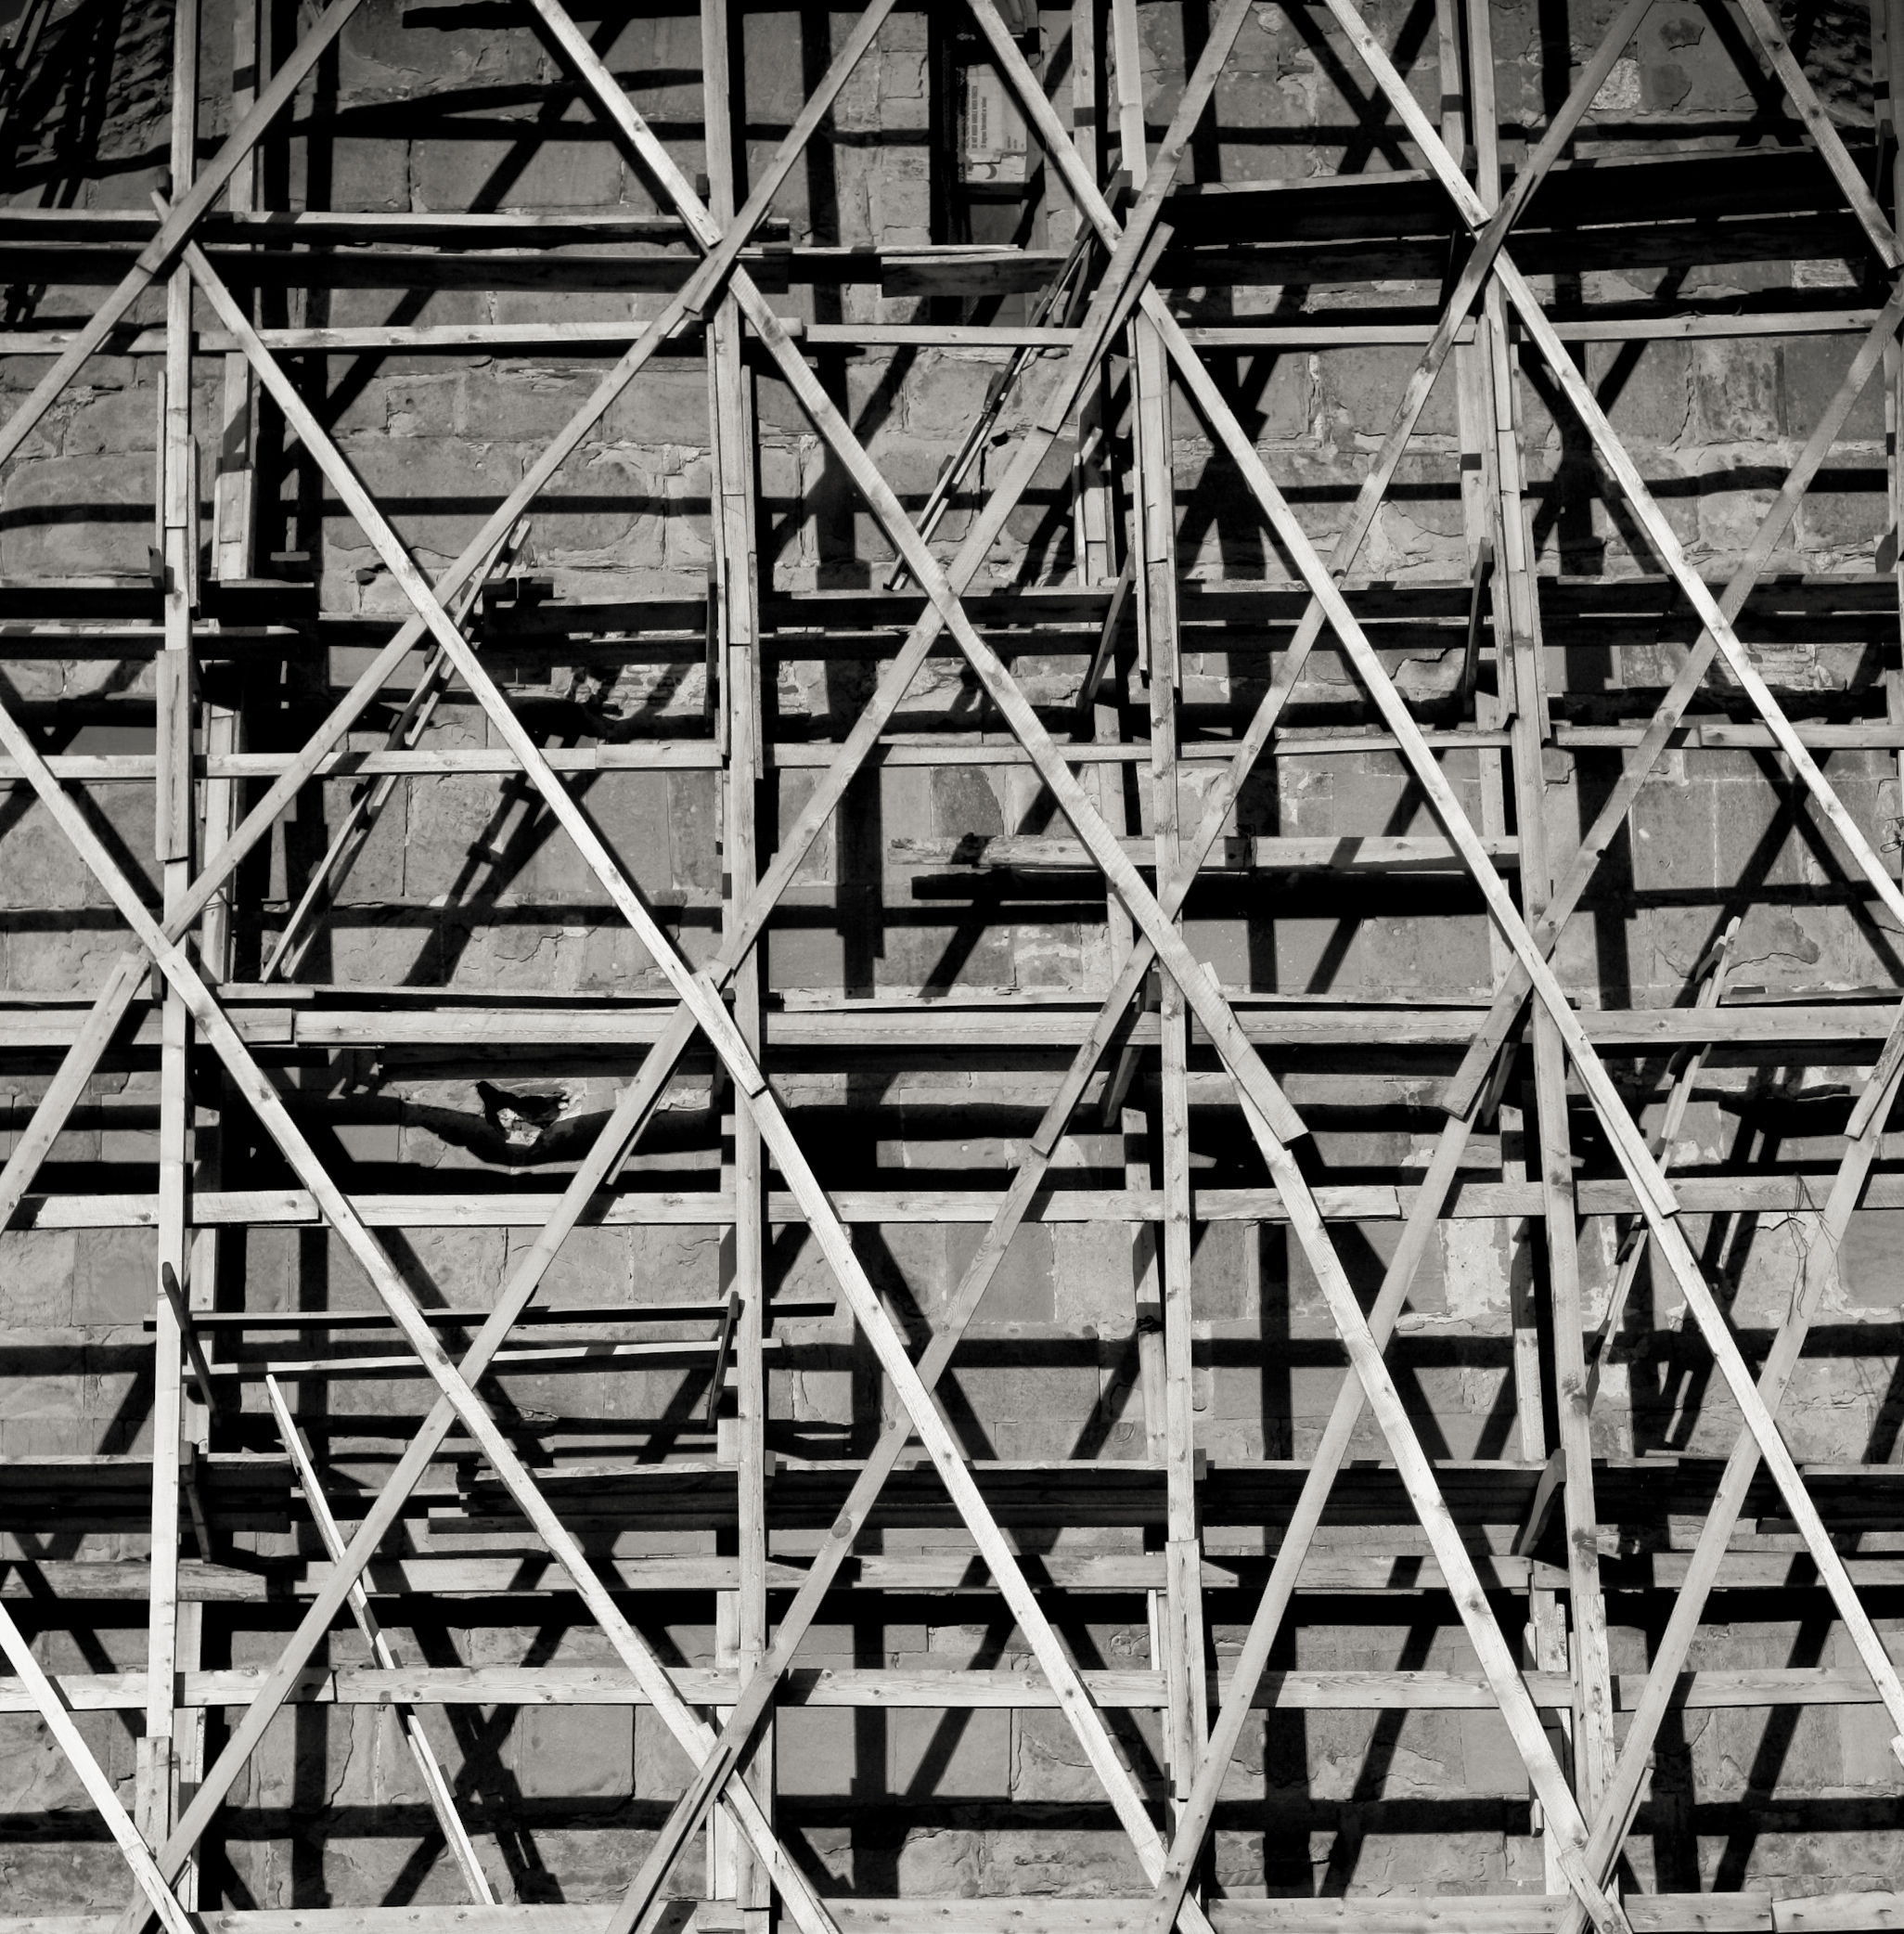
\includegraphics[width=0.95\textwidth]{rhombus.jpg}
  \begin{center}
    {\large ``In geometry, a rhombus or rhomb is a quadrilateral whose four sides all have the same length''}\par
    Foto di pursanovd\par
    \url{http://www.flickr.com/photos/pursanovd/3669422214/}\par
    Licenza: Creative Commons Attribution 2.0\par
  \end{center}
\newpage

\section{Generalità sui quadrilateri}\label{sect:generalita_quadrilateri}

\subsection{Distanza di un punto da una retta e altezza di una striscia di piano}

\begin{wrapfigure}{r}{0.3\textwidth}
\centering\begin{tikzpicture}[scale=1,font=\small]
\usetikzlibrary{calc}

\begin{scope}
\coordinate (r1) at (0.7,-2);
\coordinate (r2) at (4.3,-2);
\coordinate (s1) at (2,0.5);
\coordinate (s2) at (2,-2.5);
\coordinate (p) at (2,0);
\coordinate (h) at (intersection of r1--r2 and s1--s2);
\coordinate (q) at ($(r1)!0.75!(r2)$);

\draw[red, fill=red!20] (h) rectangle ([shift={(0.4,0.4)}]h);

\draw[thick] (r1) node[above] {$r$} -- (r2);
\draw[dashed] (p) -- (h);
\draw[fill] (p) circle (1.2pt) node [shift={(-.2,.2)}] {$P$};
\draw[fill] (h) circle (1.2pt) node [shift={(-.2,.2)}] {$H$};
\draw[fill,dashed] (p) -- (q) circle (1.2pt) node[shift={(.2,.2)}] {$Q$};

\end{scope}

\end{tikzpicture}

\end{wrapfigure}
Ricordiamo che come definizione di (\emph{misura} della) \emph{distanza di un punto da una retta} è stata presa la lunghezza del segmento congiungente il punto con il piede della perpendicolare mandata dal punto alla retta (vedi figura). Analogamente, per \emph{distanza tra due rette parallele}, detta anche \emph{altezza della striscia di piano individuata dalle due rette parallele}, si intende la distanza di un punto qualsiasi di una retta dall'altra retta. Vogliamo far vedere ora che queste definizioni sono coerenti con il concetto di distanza tra due insiemi di punti come \emph{percorso più breve} che congiunge un qualsiasi punto del primo insieme con un generico punto appartenente al secondo insieme. Se congiungiamo, infatti, un generico punto $P$ sia con $H$, piede della perpendicolare alla retta $r$, che con un altro punto $Q\in r$, viene individuato un triangolo rettangolo $PHQ$, di cui $PH$ è un cateto e $PQ$ l'ipotenusa. Dal teorema sulle disuguaglianze degli elementi di un triangolo, l'ipotenusa è certamente maggiore di un cateto in quanto lato che si oppone ad angolo maggiore (quello retto). Dunque $PH$ è il segmento di lunghezza minore tra tutti quelli che congiungono $P$ con un punto della retta $r$.

\subsection{Generalità sui poligoni}

Se un poligono ha più di tre lati, allora può anche essere concavo. Ricordiamo che la somma degli angoli interni di un quadrilatero è $360\grado$.

\begin{definizione}
Due lati non consecutivi di un quadrilatero si dicono \emph{opposti}; analogamente sono detti \emph{opposti} due angoli non adiacenti allo stesso lato.
\end{definizione}

Nella figura seguente sono rappresentati un quadrilatero concavo ($Q_1$), un generico quadrilatero convesso ($Q_2$), un quadrilatero particolare a forma di ``aquilone'' ($Q_6$) e tre quadrilateri ``notevoli'': $Q_3$ ha i lati opposti paralleli (a due a due), $Q_4$ e $Q_5$ hanno una coppia di lati opposti paralleli.

\begin{figure}[htb]
\centering% (c) 2014 Daniele Masini - d.masini.it@gmail.com
\begin{tikzpicture}[scale=1,font=\small]
\usetikzlibrary{calc}

\begin{scope}
\draw[fill=red!10] (0,0) -- (-1.3,1) -- (1.5,0) -- (-1.3,-1) -- cycle;
\node at (0.5,0) {$Q_1$};
\end{scope}

\begin{scope}[shift={(1.5cm,-1cm)}]
\draw[fill=red!10] (0,0) -- (1,1) -- (1.9,0.7) -- (1.2,-1.5) -- cycle;
\node at (1,0) {$Q_2$};
\end{scope}

\begin{scope}[shift={(-1.2cm,-3cm)}]
\draw[fill=red!10] (0,0) -- (0.5,1.5) -- (2.5,1.5) -- (2,0) -- cycle;
\node at (1.3,0.75) {$Q_3$};
\end{scope}

\begin{scope}[shift={(4cm,-.7cm)}]
\draw[fill=red!10] (0,0) -- (0,1.5) -- (1.5,1.5) -- (2,0) -- cycle;
\node at (0.9,0.75) {$Q_4$};
\end{scope}

\begin{scope}[shift={(4.3cm,-2.9cm)}]
\draw[fill=red!10] (0,0) -- (-0.5,1.5) -- (0.7,1.5) -- (2,0) -- cycle;
\node at (0.5,0.75) {$Q_5$};
\end{scope}

\begin{scope}[shift={(7.2cm,0cm)}]
\draw[fill=red!10] (0,0.4) -- (-0.8,-1.5) -- (0,-2.5) -- (0.8,-1.5) -- cycle;
\node at (0,-1.2) {$Q_6$};
\end{scope}

\end{tikzpicture}

\end{figure}

I quadrilateri che, come $Q_6$, hanno due lati consecutivi congruenti ed altri due lati consecutivi anch'essi congruenti, si dicono \emph{deltoidi}; i quadrilateri che, come $Q_3$, hanno i lati opposti paralleli si dicono \emph{parallelogrammi}; i quadrilateri che, come $Q_4$ e $Q_5$, hanno una coppia di lati opposti paralleli si dicono \emph{trapezi}.

\osservazione In analogia alla definizione di triangolo isoscele (come triangolo avente ``almeno'' due lati congruenti), alcuni autori definiscono trapezio un quadrilatero avente ``almeno'' una coppia di lati opposti paralleli: con questa definizione un parallelogramma è un particolare tipo di trapezio. Ricordiamo anche che Euclide, al contrario, classificava come trapezi tutti i quadrilateri che non fossero parallelogrammi. Noi useremo come definizione di \emph{trapezio} quella di un \emph{quadrilatero avente ``solo'' una coppia di lati opposti paralleli}. Ci riferiremo al parallelogramma come a una figura piana costituita dall'intersezione di due strisce di piano non parallele fra loro; al trapezio come intersezione tra una striscia di piano ed un angolo convesso con vertice esterno alla striscia e lati che intersecano la striscia stessa. Poiché le strisce di piano sono convesse, sia i parallelogrammi sia i trapezi, come intersezioni di figure convesse, sono convessi.

\section{Trapezio e deltoide}\label{sect:trapezio_deltoide}

Osserviamo le figure seguenti. I quadrilateri $ABCD$, $EFGH$, $IJKL$ e $MNOP$ sono trapezi perché hanno una coppia di lati opposti paralleli. Tali lati paralleli si dicono \emph{basi} e si distinguono in \emph{base maggiore} e \emph{base minore}. Gli altri lati si dicono \emph{lati obliqui}. La distanza tra le rette parallele si dice \emph{altezza} del trapezio.
Un trapezio avente i lati obliqui congruenti si dice \emph{isoscele}. Un trapezio avente un lato perpendicolare alle basi si dice \emph{rettangolo}. Un trapezio che non è né isoscele né rettangolo si dice \emph{scaleno}.

\begin{figure}[htb]
	\centering% Copyright (c) 2015 Daniele Masini - d.masini.it@gmail.com

\begin{tikzpicture}[scale=1,font=\small]
\usetikzlibrary{calc}

\begin{scope}
\draw[thick, fill=red!10] (0,0) -- (2,0) -- (2.5,-1.5) -- (-0.5,-1.5) -- cycle;
\node at (1,-2) {trapezio isoscele};
\end{scope}

\begin{scope}[shift={(4.5cm,0cm)}]
\draw[thick, fill=red!10] (0,0) -- (1.7,0) -- (2.5,-1.5) -- (0,-1.5) -- cycle;
\node at (1.25,-2) {trapezio rettangolo};
\end{scope}

\begin{scope}[shift={(-0.3cm,-2.7cm)}]
\draw[thick, fill=red!10] (0,0) -- (1.5,0) -- (3,-1.5) -- (0.5,-1.5) -- cycle;
\node at (1.5,-2) {trapezio scaleno};
\end{scope}

\begin{scope}[shift={(5cm,-2.7cm)}]
\draw[thick, fill=red!10] (0,0) -- (1.3,0) -- (2.5,-1.5) -- (-0.5,-1.5) -- cycle;
\node at (1,-2) {trapezio scaleno};
\end{scope}

\end{tikzpicture}

\end{figure}

\subsection{Proprietà del trapezio}

In ogni trapezio, gli angoli adiacenti a ciascun lato obliquo sono supplementari. Essi, infatti, sono coniugati interni rispetto alle rette delle basi tagliate dalla trasversale individuata dal lato obliquo.

In un trapezio rettangolo, gli angoli adiacenti alla base maggiore sono uno retto ed uno acuto e gli angoli adiacenti alla base minore sono uno retto ed uno ottuso. Se un trapezio avesse quattro angoli retti, i lati obliqui sarebbero entrambi perpendicolari alle basi e di conseguenza paralleli tra loro. Dunque in questo caso il trapezio risulterebbe essere un parallelogramma.

Un trapezio scaleno può avere gli angoli adiacenti alla base maggiore entrambi acuti (e quindi gli angoli adiacenti alla base minore entrambi ottusi) oppure due angoli opposti entrambi acuti e gli altri ottusi (i due tipi di trapezio scaleno sono rappresentati nella figura precedente). I quattro angoli sono comunque non congruenti, altrimenti il trapezio risulterebbe isoscele nel primo caso e un parallelogramma nel secondo caso.

\begin{wrapfigure}{r}{0.3\textwidth}
	\centering\begin{tikzpicture}[scale=1,font=\small]
\usetikzlibrary{calc}

\begin{scope}
\draw[fill=red!10] (0,0) coordinate (i) node[above] {$I$} -- (1.5,0) coordinate (l) node[above] {$L$} -- (3,-1.5) coordinate (k) node[below] {$K$} -- (0.6,-1.5) coordinate (j) node[below] {$J$} -- cycle;
\draw[dashed] (i) -- ($(j)!(i)!(k)$) coordinate (g1) node[below] {$G_1$} -- (j);
\draw[dashed] (l) -- ($(j)!(l)!(k)$) coordinate (k1) node[below] {$K_1$};
\end{scope}

\end{tikzpicture}

\end{wrapfigure}
In un trapezio isoscele, gli angoli adiacenti alla base maggiore sono acuti e quelli adiacenti alla base minore sono ottusi. 
A tal proposito, facciamo riferimento al trapezio $IJKL$ nella figura a fianco per dire che non può esistere un trapezio isoscele con due angoli acuti opposti e due angoli ottusi opposti. Infatti, se fosse $IJ\cong LK$, i triangoli $IG_1J$ e $LK_1K$ risulterebbero congruenti per il criterio particolare dei triangoli rettangoli, avendo congruenti le ipotenuse (i lati obliqui del trapezio $IJ$ e $LK$) ed una coppia di cateti (le altezze $IG_1$ e $LK_1$), da cui seguirebbe in particolare che $I\widehat{J}G_1\cong L\widehat{K}K_1$, e pertanto l'angolo in $K$ sarebbe supplementare dell'angolo in $J$, cosa che garantirebbe il parallelismo dei lati obliqui. Dunque, un ipotetico trapezio isoscele con due angoli acuti opposti sarebbe un parallelogramma.

\begin{wrapfigure}{r}{0.3\textwidth}
	\centering% (c) 2014 Daniele Masini - d.masini.it@gmail.com
\begin{tikzpicture}[scale=1,font=\small]
\usetikzlibrary{calc}

\begin{scope}
\draw[fill=red!10] (0.1,0) coordinate (b) node[above] {$B$} -- (1.9,0) coordinate (c) node[above] {$C$} -- (2.5,-1.5) coordinate (d) node[below] {$D$} -- (-0.5,-1.5) coordinate (a) node[below] {$A$} -- cycle;
\draw[dashed] (b) -- ($(a)!(b)!(d)$) coordinate (d1) node[below] {$D_1$};
\draw[dashed] (c) -- ($(a)!(c)!(d)$) coordinate (e1) node[below] {$E_1$};
\draw[dashed] (b) -- (d);
\draw[dashed] (a) -- (c);
\end{scope}


\end{tikzpicture}

\end{wrapfigure}
Inoltre, se il trapezio è isoscele, gli angoli adiacenti a ciascuna delle basi sono congruenti. 
Infatti, in riferimento al trapezio $ABCD$, traccia le altezze $BD_1$ e $CE_1$ (tra loro congruenti perché entrambe rappresentano la distanza tra due rette parallele), i triangoli $AD_1B$ e $E_1DC$ risultano congruenti per il criterio particolare dei triangoli rettangoli, avendo congruenti le ipotenuse (i lati obliqui del trapezio) ed una coppia di cateti (le altezze del trapezio). Pertanto i rimanenti elementi risultano ordinatamente congruenti: $B\widehat{A}D\cong A\widehat{D}C$, $A\widehat{B}D_1\cong D\widehat{C}E_1$, $AD_1\cong E_1D$.

Dunque sono congruenti  anche le proiezioni dei lati obliqui sulla base maggiore. 
Quindi anche $A\widehat{B}C\cong B\widehat{C}D$ in quanto somme di angoli congruenti $A\widehat{B}D_1+\widehat{R}\cong D\widehat{C}E_1+\widehat{R}$.

In un trapezio isoscele, inoltre, anche le due diagonali sono congruenti. Infatti, in riferimento sempre al trapezio $ABCD$ in figura, i triangoli $ABC$ e $DCB$ risultano congruenti per il primo criterio, avendo $BC$ in comune, $AB\cong CD$ per ipotesi e gli angoli compresi (adiacenti alla base minore) congruenti per quanto appena dimostrato. Di conseguenza, i rimanenti elementi sono ordinatamente congruenti, in particolare i terzi lati (che sono, appunto, le diagonali $AC$ e $BD$ del trapezio).

\subsection{Proprietà del deltoide}

\begin{wrapfigure}{r}{0.3\textwidth}
	\centering\begin{tikzpicture}[scale=0.8,font=\small]
\usetikzlibrary{calc}

\begin{scope}
\draw[fill=red!10] (0,0) coordinate (q) node[above] {$Q$} -- (1.5,-1.5) coordinate (t) node[right] {$T$} -- (0,-4) coordinate (s) node[below] {$S$} -- (-1.5,-1.5) coordinate (r) node[left] {$R$} -- cycle;
\coordinate (h) at (intersection of r--t and q--s);
\draw[dashed] (q) -- (s);
\draw[dashed] (r) -- (t);
\draw[fill] (h) circle (1.2pt) node[shift={(0.2,0.2)}] {$H$};
\end{scope}


\end{tikzpicture}

\end{wrapfigure}
Il poligono $QRST$ nella figura a fianco è un deltoide, ha i lati a due a due congruenti $QR\cong QT$ e $RS\cong TS$. Tracciamo le diagonali $QS$ ed $RT$. I triangoli $QRT$ e $STR$ sono isosceli sulla base comune $RT$. Dunque, se chiamiamo $H$ il punto medio di $RT$, $QH$ ed $SH$ sono mediane, bisettrici e altezze (relative alla base ed agli angoli al vertice dei due triangoli isosceli), per cui $QS$ è perpendicolare ad $RT$ e passa per il punto $H$. Quindi le due diagonali sono perpendicolari e si incontrano nel punto medio di $RT$. Inoltre i triangoli $SQR$ ed $STQ$ sono congruenti per il terzo criterio, pertanto $Q\widehat{R}S\cong Q\widehat{T}S$.

I quattro lati di un deltoide non potrebbero essere tutti congruenti, in quanto, dalla congruenza degli angoli opposti banalmente deducibile, risulterebbero i lati opposti paralleli, e quindi il deltoide sarebbe un parallelogramma. Non è al contrario escluso che un angolo possa essere retto (ma non più di uno, altrimenti il deltoide sarebbe un parallelogramma), mentre gli angoli ottusi possono essere uno, due o tre (come pure gli angoli acuti).

Lasciamo al lettore il compito di provare queste semplici proprietà, costruendo vari tipi di deltoidi.


\section{Proprietà dei parallelogrammi}\label{sect:proprieta_parallelogrammi}

Ricordiamo che, per definizione, un parallelogramma è un quadrilatero che ha i lati opposti paralleli.

\begin{teorema}
In ogni parallelogramma:
\begin{enumerate*}
\item gli angoli adiacenti allo stesso lato (a ciascun lato) sono supplementari;
\item gli angoli opposti sono congruenti;
\item ciascuna diagonale divide il parallelogramma in due triangoli congruenti;
\item i lati opposti sono congruenti;
\item le diagonali si dividono scambievolmente per metà. 
\end{enumerate*}
\end{teorema}

\noindent Ipotesi: $AB\parallel CD$, $AD\parallel BC$.

\begin{figure}[htb]
	\centering\begin{tikzpicture}[scale=1,font=\small]
\usetikzlibrary{calc}

\begin{scope}
\draw[fill=red!10] (0,0) coordinate (a) node[below] {$A$} -- (2.5,0) coordinate (b) node[below] {$B$} -- (3,1.5) coordinate (c) node[above] {$C$} -- (0.5,1.5) coordinate (d) node[above] {$D$} -- cycle;
\coordinate (m) at (intersection of d--b and a--c);
\draw[dashed] (a) -- (c);
\draw[dashed] (d) -- (b);
\draw[fill] (m) circle (1.2pt) node[above] {$M$};
\end{scope}


\end{tikzpicture}

\end{figure}

\begin{proof}~\\
\begin{enumerate*}
		
\item Tesi: $D\widehat{A}B+A\widehat{B}C\cong\pi$, $A\widehat{B}C+B\widehat{C}D\cong\pi$, $B\widehat{C}D+C\widehat{D}A\cong\pi$ ($\pi$ è l'angolo piatto).\\
Se $AB\parallel CD$, gli angoli in $A$ e $D$ sono supplementari, e così pure gli angoli in $B$ e $C$, in quanto coniugati interni rispetto alle due rette parallele tagliate rispettivamente dalle trasversali $AD$ e $BC$. Analogamente, se $AD\parallel BC$, gli angoli in $A$ e $B$ sono supplementari, ed anche gli angoli in $C$ e $D$. La tesi 1 è pertanto dimostrata.

\item Tesi: $A\widehat{B}C\cong C\widehat{D}A$, $D\widehat{A}B\cong B\widehat{C}D$.\\
Dunque, se è vera l'ipotesi, possiamo considerare verificate le congruenze della tesi 1. Da queste segue che gli angoli opposti sono congruenti in quanto supplementari dello stesso angolo: gli angoli in $A$ e $C$ sono supplementari entrambi dell'angolo in $B$, gli angoli in $B$ e in $D$ sono entrambi supplementari dell'angolo in $A$. La tesi 2 è pertanto dimostrata.

\item Tesi: $ABC\cong CDA$, $DAB\cong BCD$.\\
Tracciamo ora una diagonale, ad esempio $AC$, e consideriamo i due triangoli che si vengono a formare, $ABC$ e $ACD$. Essendo $AB\parallel CD$, risulta $D\widehat{C}A\cong C\widehat{A}B$ ed essendo $AD\parallel BC$, risulta $D\widehat{A}C\cong A\widehat{C}B$, in quanto sono coppie di angoli alterni interni, i primi rispetto alle rette $AB$ e $CD$ tagliate dalla trasversale $AC$, gli altri rispetto alle rette parallele $AD$ e $BC$ tagliate dalla trasversale $AC$. I due triangoli dunque, avendo in comune il lato $AC$, risultano congruenti per il secondo criterio. Analogamente, applicando il ragionamento precedente ai triangoli $ABD$ e $DBC$ dopo aver tracciato la diagonale $DB$, concludiamo che anche i due triangoli $ADB$ e $DBC$ risultano congruenti per il secondo criterio. Pertanto la tesi 3 è dimostrata.

\item Tesi: $AB\cong CD$, $AD\cong BC$.\\
Dunque, se è vera l'ipotesi, possiamo considerare verificate le congruenze della tesi 3. Dalla congruenza dei triangoli $ABC$ e $CDA$ segue la congruenza dei lati $AB$ e $CD$, dalla congruenza dei triangoli $DAB$ e $BCD$ segue la congruenza dei lati $AD$ e $BC$. Pertanto la tesi 4 è dimostrata.

\item Tesi: $AM\cong MC$, $DM\cong MB$.\\
Dopo aver tracciato entrambe le diagonali, chiamiamo $M$ il loro punto di intersezione. Confrontiamo i triangoli $ABM$ e $CDM$: essi risultano congruenti per il secondo criterio, in quanto $AB\cong CD$ (tesi 4), $D\widehat{A}C\cong A\widehat{C}B$ e $D\widehat{C}A\cong C\widehat{A}B$ (come visto nel punto 3 della dimostrazione). Quindi anche i rimanenti elementi risultano ordinatamente congruenti, in particolare $AM\cong MC$ e $DM\cong MB$. Pertanto anche la tesi 5 è dimostrata.
\end{enumerate*}
\end{proof}

Il teorema precedente è invertibile. Precisamente vale il teorema seguente:
\begin{teorema}
Se in un quadrilatero è verificata una delle seguenti ipotesi:
\begin{enumerate*}
\item gli angoli adiacenti allo stesso lato (a ciascun lato) sono supplementari;
\item gli angoli opposti sono congruenti;
\item ciascuna diagonale divide il quadrilatero in due triangoli congruenti;
\item i lati opposti sono congruenti;
\item le diagonali si dividono scambievolmente per metà;
\item due lati opposti sono paralleli e congruenti;
\end{enumerate*}
allora il quadrilatero è un parallelogramma.
\end{teorema}

\begin{figure}[htb]
	\centering\begin{tikzpicture}[scale=1,font=\small]
\usetikzlibrary{calc}

\begin{scope}
\draw[fill=red!10] (0,0) coordinate (a) node[below] {$A$} -- (2.5,0) coordinate (b) node[below] {$B$} -- (3,1.7) coordinate (c) node[above] {$C$} -- (0.5,1.7) coordinate (d) node[above] {$D$} -- cycle;
\coordinate (o) at (intersection of d--b and a--c);
\draw[dashed] (a) -- (c);
\draw[dashed] (d) -- (b);
\draw[fill] (o) circle (1.2pt) node[above] {$O$};
%\node at (1.5,-1) {(a)};
\end{scope}

%\begin{scope}[xshift=5cm]
%\draw[fill=red!10] (0,0) coordinate (e) node[below] {$E$} -- (2.5,0) coordinate (f) node[below] {$F$} -- (3,1.7) coordinate (g) node[above] {$G$} -- (0.5,1.7) coordinate (h) node[above] {$H$} -- cycle;
%\coordinate (o) at (intersection of d--b and a--c);
%\draw[dashed] (e) -- (g);
%\draw[dashed] (f) -- (h);
%\draw[fill] (o) circle (1.2pt) node[left] {$O$};
%\node at (1.5,-1) {(b)};
%\end{scope}


\end{tikzpicture}

\end{figure}

\begin{proof}~\\
\begin{enumerate*}
\item Sia per ipotesi $D\widehat{A}B+A\widehat{B}C\cong \pi$ (dove $\pi$ è l'angolo piatto). Tali angoli, rispetto alle rette $AD$ ed $BC$ tagliate dalla trasversale $AB$ sono coniugati interni, allora per quanto visto nel capitolo precedente sul parallelismo, le rette $AD$ e $BC$ sono parallele perché formano angoli coniugati interni supplementari con la trasversale $AB$. Analogamente, se $A\widehat{B}C+B\widehat{C}D\cong \pi$, le rette $AB$ ed $DC$ sono parallele. Dunque $ABCD$ è un parallelogramma, avendo i lati opposti paralleli.
\item Poiché la somma degli angoli interni di un quadrilatero misura $360\grado$, se gli angoli opposti sono congruenti, vuol dire che $D\widehat{A}B+A\widehat{B}C+B\widehat{C}D+C\widehat{D}A\cong 2D\widehat{A}B+2A\widehat{B}C\cong 2\pi$, per cui $D\widehat{A}B+A\widehat{B}C\cong\pi$, cioè gli angoli adiacenti allo stesso lato sono supplementari e per la dimostrazione precedente $ABCD$ è un parallelogramma.
\item Essendo i triangoli $ABC$ e $BDC$ congruenti, l'angolo $A\widehat{B}D$ risulta congruente all'angolo $B\widehat{D}C$ ed essendo questi angoli alterni interni rispetto alle rette $AB$ e $CD$ tagliate dalla trasversale $BD$ allora le due rette $AB$ e $CD$ saranno parallele. In maniera analoga $A\widehat{D}B\cong D\widehat{B}C$ e quindi, essendo alterni interni rispetto alle rette $BC$ e $AD$ intersecate dalla trasversale $BD$ si ha che anche $BC\parallel AD$. Quindi $ABCD$ è un parallelogramma.
%\item Sia $FH$ una diagonale del quadrilatero $EFGH$, figura (b), allora i vertici $E$ e $G$ cadranno su semipiani opposti rispetto alla retta $FH$. Nel caso in cui i due triangoli $FHE$ e $FHG$, oltre che congruenti, sono isosceli sulla base $FH$, il quadrilatero $EFGH$ ha gli angoli opposti congruenti, per cui è un parallelogramma per la tesi 2. Se, al contrario, $FHE$ e $FHG$ non sono isosceli sulla base $FH$, allora dobbiamo considerare due sottocasi distinti, evidenziati in figura, con quattro diversi quadrilateri. Se fosse $EH\cong HG$ e $EF\cong FG$, la figura risulterebbe un deltoide e l'altra diagonale $EG$ non dividerebbe il quadrilatero in due triangoli congruenti. Rimane l'altro sottocaso possibile, $EF\cong HG$ e $EH\cong FG$, ed inoltre $A\widehat{D}B\cong D\widehat{B}C$, $A\widehat{B}D\cong B\widehat{D}C$ e $D\widehat{A}B\cong B\widehat{C}D$, pertanto il quadrilatero risulta essere un parallelogramma per la 2. Dunque in ogni caso possibile la tesi è dimostrata.
\item Consideriamo la diagonale $AC$. Il quadrilatero $ABCD$ è diviso in due triangoli $ABC$ e $ACD$ congruenti per il terzo criterio. Pertanto $A\widehat{C}D\cong C\widehat{A}B$ e $A\widehat{C}B\cong C\widehat{A}D$, coppie di angoli alterni interni, nell'ordine rispetto alle rette $AB$ e $CD$ e rispetto alle rette $AD$ ed $BC$, tagliate dalla trasversale $AC$. Dunque i lati opposti del quadrilatero $ABCD$ risultano paralleli, cioè è un parallelogramma.
\item Detto $O$ il punto di incontro delle diagonali, i triangoli $OAB$ ed $OCD$ risultano congruenti per il primo criterio, in quanto $OA\cong OC$, $OD\cong OB$ e gli angoli tra essi compresi sono congruenti perché opposti al vertice. Di conseguenza, risulta anche $D\widehat{C}A\cong C\widehat{A}B$, che sono angoli alterni interni rispetto alle rette $DC$ ed $AB$ tagliate dalla trasversale $AC$, pertanto $DC\parallel AB$. Analogamente, considerando i triangoli congruenti $OBC$ ed $ODA$ si ha anche $BC\parallel AD$. Dunque $ABCD$ è un parallelogramma.
\item Supponiamo $AB$ e $CD$ paralleli e congruenti. Tracciata la diagonale $AC$, risulta $D\widehat{C}A\cong C\widehat{A}B$ e dunque i triangoli $ACD$ e $CAB$ risultano congruenti per il primo criterio. Di conseguenza risulta $AD\cong BC$, per cui il quadrilatero ha anche l'altra coppia di lati opposti congruenti. $ABCD$ è dunque un parallelogramma per la 4.
\end{enumerate*}
\end{proof}

\section{Parallelogrammi particolari}\label{sect:parallelogrammi_particolari}

I parallelogrammi possono essere sia equiangoli sia equilateri.

\noindent\begin{minipage}{0.7\textwidth}\parindent15pt
Se un parallelogramma è equiangolo, dato che la somma degli angoli interni è $360\grado$, deve avere quattro angoli retti: questo succede quando due lati opposti, paralleli tra loro, sono perpendicolari all’altra coppia di lati opposti. Un tale parallelogramma si chiama \emph{rettangolo}.

Se un parallelogramma è equilatero, vuol dire che ciascuna diagonale lo divide in due triangoli isosceli. Un tale parallelogramma si chiama \emph{rombo}.

Un parallelogramma sia equiangolo sia equilatero deve essere contemporaneamente un rettangolo ed un rombo: l'unico tipo di quadrilatero regolare, il \emph{quadrato}. Infatti un quadrilatero, per essere regolare, deve necessariamente avere quattro angoli retti; è quindi un parallelogramma, prima ancora che un rettangolo, perché due angoli retti, oltre ad essere congruenti, sono anche supplementari; inoltre è un rombo in quanto è un parallelogramma con quattro lati congruenti.
\end{minipage}\hfil
\begin{minipage}{0.3\textwidth}
	\centering% Copyright (c) 2015 Daniele Masini - d.masini.it@gmail.com

\begin{tikzpicture}[scale=1,font=\small]
\usetikzlibrary{calc}

\begin{scope}
\draw[thick, fill=red!10] (0,0) coordinate (a) -- (2.5,0) coordinate (b) -- (2.5,1.3) coordinate (c) -- (0,1.3) coordinate (d) -- cycle;
\node at (1.25,-0.3) {rettangolo};
\end{scope}

\end{tikzpicture}
\\~\\
	\centering\begin{tikzpicture}[scale=1,font=\small]
\usetikzlibrary{calc}

\begin{scope}
\draw[fill=red!10] (0,0) coordinate (a) -- (1.5,-0.7) coordinate (b) -- (3,0) coordinate (c) -- (1.5,0.7) coordinate (d) -- cycle;
\node at (1.5,-1) {rombo};
\end{scope}

\end{tikzpicture}
\\~\\
	\centering\begin{tikzpicture}[scale=1,font=\small]
\usetikzlibrary{calc}

\begin{scope}
\draw[thick, fill=red!10] (0,0) coordinate (a) -- (1.5,0) coordinate (b) -- (1.5,1.5) coordinate (c) -- (0,1.5) coordinate (d) -- cycle;
\node at (0.75,-0.3) {quadrato};
\end{scope}

\end{tikzpicture}

\end{minipage}

A parte le proprietà particolari insite nelle stesse definizioni, il rettangolo e il rombo si distinguono tra loro e dagli altri parallelogrammi per alcune proprietà riguardanti le diagonali. Naturalmente il quadrato gode delle proprietà sia del rettangolo sia del rombo.
Ricordiamo che in un parallelogramma le diagonali si dividono scambievolmente per metà. Ora mostreremo che in un rettangolo le diagonali sono congruenti ed in un rombo sono perpendicolari.

\begin{teorema}
In ogni rettangolo le diagonali sono congruenti. Viceversa, se un parallelogramma ha le diagonali congruenti, allora è un rettangolo.
\end{teorema}

\begin{figure}[htb]
	\centering\begin{tikzpicture}[scale=1,font=\small]
\usetikzlibrary{calc}

\begin{scope}
\draw[fill=red!10] (0,0) coordinate (a) node[left] {$R$} -- (2.5,0) coordinate (b) node[right] {$P$} -- (2.5,1.3) coordinate (c) node[right] {$Q$} -- (0,1.3) coordinate (d) node[left] {$S$} -- cycle;
\draw[blue] (a) -- (c);
\draw[blue] (b) -- (d);
\end{scope}

\end{tikzpicture}

\end{figure}

\begin{proof}
Sia $RPQS$ un rettangolo; tracciate le diagonali $RQ$ e $PS$, confrontiamo i triangoli $SRP$ e $RPQ$. Tali triangoli rettangoli hanno il cateto $RP$ in comune ed hanno gli altri cateti, $SR$ e $PQ$, rispettivamente congruenti in quanto lati opposti di un rettangolo. Dunque $SRP$ e $RPQ$ sono congruenti per il primo criterio e di conseguenza devono avere congruenti anche le ipotenuse $SP$ e $RQ$, le quali sono le diagonali del rettangolo.

Sia $RPQS$ un parallelogramma avente le diagonali $RQ$ e $PS$ congruenti, sempre confrontando i triangoli $SRP$ e $RPQ$, possiamo affermare che tali triangoli sono congruenti per il terzo criterio, perché hanno il lato $RP$ in comune, i lati $RS$ e $QP$ congruenti in quanto lati opposti di un parallelogramma ed i lati $SP$ e $RQ$ congruenti per ipotesi. Dunque anche gli angoli devono essere ordinatamente congruenti, in particolare  perché opposti ai lati congruenti $SP$ e $RQ$. Ma tali angoli sono anche supplementari in quanto adiacenti allo stesso lato $RP$ di un parallelogramma e pertanto devono risultare retti. Dunque il quadrilatero $RPSQ$ è un rettangolo.
\end{proof}

\begin{teorema}
In ogni rombo le diagonali sono perpendicolari e sono anche bisettrici degli angoli aventi per vertici i loro estremi. Viceversa, se un parallelogramma ha le diagonali perpendicolari è un rombo; inoltre, se un angolo di un parallelogramma è diviso a metà dalla diagonale passante per il suo vertice, allora il parallelogramma è un rombo.
\end{teorema}

\begin{figure}[htb]
	\centering% Copyright (c) 2015 Daniele Masini - d.masini.it@gmail.com

\begin{tikzpicture}[scale=1.2,font=\small]
\usetikzlibrary{calc}

\begin{scope}
\draw[fill=red!10] (0,0) coordinate (a) node[left] {$K$} -- (1.5,-0.7) coordinate (b) node[below] {$J$} -- (3,0) coordinate (c) node[right] {$H$} -- (1.5,0.7) coordinate (d) node[above] {$G$} -- cycle;
\draw[blue] (a) -- (c);
\draw[blue] (b) -- (d);
\end{scope}

\end{tikzpicture}

\end{figure}

\begin{proof}
Notiamo che, in ciascuna delle fasi della dimostrazione, è tra le ipotesi del teorema che $JHGK$ sia un parallelogramma. Ricordiamo che le diagonali di $JHGK$ vengono divise a metà dal loro punto di intersezione, che chiamiamo $M$, per cui risulta $JM\cong MG$ e $HM\cong MK$.
\begin{enumeratea}
\item Se supponiamo che $JHGK$ sia un rombo, i triangoli $JHG$, $HGK$, $GKJ$ e $KJH$ risultano isosceli, per cui le mediane $HM$, $GM$, $KM$ e $JM$ sono anche altezze e bisettrici, per cui la prima parte del teorema è dimostrata.
\item Se supponiamo che $JG$ e $HK$ siano perpendicolari, in particolare i triangoli rettangoli $JHM$, $HGM$, $GKM$ e $KJM$ risultano congruenti per il primo criterio, avendo congruenti i cateti. Dunque risultano congruenti anche le ipotenuse, che sono i lati del parallelogramma $JHGK$, il quale pertanto risulta essere un rombo.
\item Se supponiamo ad esempio $K\widehat{G}J\cong J\widehat{G}H$, essendo anche $K\widehat{G}J\cong G\widehat{J}H$ in quanto alterni interni rispetto alle rette parallele $KG$ e $JH$ tagliate dalla trasversale $GJ$, dalla proprietà transitiva della congruenza segue che $G\widehat{J}H\cong J\widehat{G}H$, per cui il triangolo $JGH$ risulta isoscele sulla base $JG$. Dunque il parallelogramma $JHGK$ ha due lati consecutivi congruenti, e quindi i quattro lati congruenti, ed è pertanto un rombo.
\end{enumeratea}
\end{proof}

I teoremi precedenti si estendono automaticamente ai quadrati.
\begin{corollario}
Le diagonali di un quadrato sono fra loro congruenti e perpendicolari e dividono per metà gli angoli. Viceversa, se un parallelogramma ha le diagonali congruenti e perpendicolari, allora è un quadrato; inoltre, se le diagonali di un parallelogramma sono congruenti ed un angolo è diviso a metà da una diagonale, allora il parallelogramma è un quadrato.
\end{corollario}

\section{Corrispondenza di Talete}\label{sect:corrispondenza_talete}

\begin{definizione}
Nel piano, si definisce \emph{fascio improprio di rette} un insieme di rette tutte parallele tra loro.
\end{definizione}

Ricordiamo che una retta contenuta nello stesso piano e non appartenente al fascio improprio è necessariamente incidente rispetto a ciascuna retta del fascio ed ha quindi uno ed un solo punto in comune con ogni singola retta del fascio: una tale retta è dunque una trasversale.

\noindent\begin{minipage}{0.65\textwidth}\parindent15pt
Dato un fascio di rette parallele $a$, $b$, $c$, $d$, \ldots{}, considerate due generiche trasversali, $t_1$ e $t_2$, è possibile definire una funzione tra l'insieme dei punti di una trasversale e quello dei punti dell'altra trasversale, che associ a ciascun punto di $t_1$ il punto di $t_2$ che appartiene alla medesima retta del fascio (ad esempio al punto $A_1$ si associa il punto $A_2$ se, come nella figura a fianco, $A_1 = a \cap t_1$ e $A_2 = a \cap t_2$). Tale funzione è una corrispondenza biunivoca e si estende facilmente ai segmenti: infatti l'immagine del segmento $A_1B_1$ è il segmento $A_2B_2$ (se, come nella figura, anche gli estremi $B_1$ e $B_2$ appartengono alla stessa retta $b$ del fascio).
La corrispondenza biunivoca così definita tra punti e tra segmenti di due trasversali che tagliano un fascio di rette parallele è nota come \emph{corrispondenza di Talete}.
\end{minipage}\hfil
\begin{minipage}{0.35\textwidth}
	\centering\begin{tikzpicture}[scale=1,font=\small]
\usetikzlibrary{calc}

\begin{scope}
\coordinate (a1) at (0,-0.3);
\coordinate (a2) at (4,-0.3);
\coordinate (b1) at (0,-1.5);
\coordinate (b2) at (4,-1.5);
\coordinate (c1) at (0,-2.25);
\coordinate (c2) at (4,-2.25);
\coordinate (d1) at (0,-3);
\coordinate (d2) at (4,-3);
\coordinate (t11) at (2,0.5);
\coordinate (t12) at (0.5,-3.5);
\coordinate (t21) at (3,0.5);
\coordinate (t22) at (3.5,-3.5);
\coordinate (A1) at (intersection of a1--a2 and t11--t12);
\coordinate (A2) at (intersection of a1--a2 and t21--t22);
\coordinate (B1) at (intersection of b1--b2 and t11--t12);
\coordinate (B2) at (intersection of b1--b2 and t21--t22);
\coordinate (C1) at (intersection of c1--c2 and t11--t12);
\coordinate (C2) at (intersection of c1--c2 and t21--t22);
\coordinate (D1) at (intersection of d1--d2 and t11--t12);
\coordinate (D2) at (intersection of d1--d2 and t21--t22);

\draw (a1) node[above] {$a$} -- (a2);
\draw (b1) node[above] {$b$} -- (b2);
\draw (c1) node[above] {$c$} -- (c2);
\draw (d1) node[above] {$d$} -- (d2);
\draw (t11) node[above] {$t_1$} -- (t12);
\draw (t21) node[above] {$t_2$} -- (t22);
\draw (A1) circle (1.2pt) node[shift={(-0.2,0.2)}] {$A_1$};
\draw (A2) circle (1.2pt) node[shift={(0.2,0.2)}] {$A_2$};
\draw (B1) circle (1.2pt) node[shift={(-0.2,0.2)}] {$B_1$};
\draw (B2) circle (1.2pt) node[shift={(0.2,0.2)}] {$B_2$};
\draw (C1) circle (1.2pt) node[shift={(-0.2,0.2)}] {$C_1$};
\draw (C2) circle (1.2pt) node[shift={(0.2,0.2)}] {$C_2$};
\draw (D1) circle (1.2pt) node[shift={(-0.2,0.2)}] {$D_1$};
\draw (D2) circle (1.2pt) node[shift={(0.2,0.2)}] {$D_2$};

\end{scope}

\end{tikzpicture}

\end{minipage}

\begin{teorema}\label{teo:Talete}
Dato un fascio di rette parallele tagliato da due trasversali, a segmenti congruenti su una trasversale corrispondono segmenti congruenti sull'altra trasversale.
\end{teorema}

\noindent Ipotesi: $A\parallel b\parallel c\parallel d$, $t_1$ e $t_2$ trasversali, $A_1B_1\cong C_1D_1$.\tab Tesi: $A_2B_2\cong C_2D_2$.

\begin{figure}[htb]
	\centering% Copyright (c) 2015 Daniele Masini - d.masini.it@gmail.com

\begin{tikzpicture}[scale=0.9,font=\small, extended line/.style={shorten >=-#1,shorten <=-#1},
  extended line/.default=0.5cm]
\usetikzlibrary{calc}

\begin{scope}
\coordinate (a1) at (0,-.25);
\coordinate (a2) at (6,-.25);
\coordinate (b1) at (0,-1);
\coordinate (b2) at (6,-1);
\coordinate (c1) at (0,-2.25);
\coordinate (c2) at (6,-2.25);
\coordinate (d1) at (0,-3);
\coordinate (d2) at (6,-3);
\coordinate (t11) at (1.8,0.5);
\coordinate (t12) at (0.5,-3.5);
\coordinate (t21) at (3,0.5);
\coordinate (t22) at (5.5,-3.5);
\coordinate (A1) at (intersection of a1--a2 and t11--t12);
\coordinate (A2) at (intersection of a1--a2 and t21--t22);
\coordinate (B1) at (intersection of b1--b2 and t11--t12);
\coordinate (B2) at (intersection of b1--b2 and t21--t22);
\coordinate (C1) at (intersection of c1--c2 and t11--t12);
\coordinate (C2) at (intersection of c1--c2 and t21--t22);
\coordinate (D1) at (intersection of d1--d2 and t11--t12);
\coordinate (D2) at (intersection of d1--d2 and t21--t22);
\path (A2) -- +($(B1)-(A1)$) coordinate (B);
\path (C2) -- +($(D1)-(C1)$) coordinate (D);
\draw[dashed, extended line] (A2) -- (B) node[shift={(-.3,-.4)}] {$r$};
\draw[dashed, extended line] (C2) -- (D) node[shift={(-.3,-.4)}] {$s$};

\draw (a1) node[above] {$a$} -- (a2);
\draw (b1) node[above] {$b$} -- (b2);
\draw (c1) node[above] {$c$} -- (c2);
\draw (d1) node[above] {$d$} -- (d2);
\draw (t11) node[above] {$t_1$} -- (t12);
\draw (t21) node[above] {$t_2$} -- (t22);
\draw[thick, blue] (A1) -- (B1);
\draw[thick, blue] (C1) -- (D1);
\draw[thick, red] (A2) -- (B2);
\draw[thick, red] (C2) -- (D2);
\draw[fill] (A1) circle (1.2pt) node[shift={(-0.2,0.2)}] {$A_1$};
\draw[fill] (A2) circle (1.2pt) node[shift={(0.3,0.2)}] {$A_2$};
\draw[fill] (B1) circle (1.2pt) node[shift={(-0.2,0.2)}] {$B_1$};
\draw[fill] (B2) circle (1.2pt) node[shift={(0.2,0.2)}] {$B_2$};
\draw[fill] (C1) circle (1.2pt) node[shift={(-0.2,0.2)}] {$C_1$};
\draw[fill] (C2) circle (1.2pt) node[shift={(0.3,0.2)}] {$C_2$};
\draw[fill] (D1) circle (1.2pt) node[shift={(-0.2,0.2)}] {$D_1$};
\draw[fill] (D2) circle (1.2pt) node[shift={(0.2,0.2)}] {$D_2$};
\draw[fill] (B) circle (1.2pt) node[shift={(-0.2,0.2)}] {$B$};
\draw[fill] (D) circle (1.2pt) node[shift={(-0.2,0.2)}] {$D$};

\end{scope}

\end{tikzpicture}

\end{figure}

\begin{proof}
Se fosse $t_1\parallel t_2$, allora la tesi seguirebbe facilmente dalle proprietà dei quadrilateri particolari e dalla proprietà transitiva della congruenza. Infatti i quadrilateri $A_1B_1B_2A_2$ e $C_1D_1D_2C_2$ sarebbero due parallelogrammi, ed avrebbero dunque i lati opposti congruenti.
Altrimenti, tracciamo la retta $r$ passante per $A_2$ e la retta $s$ passante per $C_2$, entrambe parallele a $t_1$; chiamiamo $B$ il punto di intersezione tra $b$ ed $r$ e $D$ il punto di intersezione tra $d$ ed $s$.
I quadrilateri $A_1B_1BA_2$ e $C_1D_1DC_2$ sono due parallelogrammi, per cui da $A_1B_1\cong C_1D_1$ segue, per la proprietà transitiva della congruenza, $A_2B\cong C_2D$. Dunque, se confrontiamo i triangoli $A_2BB_2$ e $C_2DD_2$, questi risultano congruenti per il secondo criterio (generalizzato), in quanto gli angoli in $A_2$ e in $C_2$ sono corrispondenti rispetto alle rette parallele $r$ e $s$ tagliate dalla trasversale $t_2$, mentre gli angoli in $B_2$ e $D_2$ sono corrispondenti rispetto alle rette parallele $b$ e $d$ tagliate dalla trasversale $t_2$ e pertanto congruenti. Di conseguenza $A_2B_2\cong C_2D_2$.
\end{proof}

\noindent\begin{minipage}{0.6\textwidth}\parindent15pt
\osservazione Nella figura precedente, i trapezi $A_1B_1B_2A_2$ e $C_1D_1D_2C_2$ sono stati ``decomposti'' in parallelogrammi e triangoli. La sostanza del teorema non cambia però se le figure che si ottengono sono diverse.
Nella figura seguente, si considerino, oltre alla corrispondenza tra i segmenti su $t_1$ e $t_2$, anche le corrispondenze tra i segmenti su $t_1$ e $t_3$ (parallele) e quella tra i segmenti su $t_2$ e $t_3$ (con $C_3$ coincidente con $C_2$).
\end{minipage}\hfil
\begin{minipage}{0.4\textwidth}
	\centering\begin{tikzpicture}[scale=.7,font=\small, extended line/.style={shorten >=-#1,shorten <=-#1},
  extended line/.default=0.5cm]
\usetikzlibrary{calc}

\begin{scope}
\coordinate (a1) at (-0.3,-.25);
\coordinate (a2) at (6,-.25);
\coordinate (b1) at (-0.3,-1);
\coordinate (b2) at (6,-1);
\coordinate (c1) at (-0.3,-2.25);
\coordinate (c2) at (6,-2.25);
\coordinate (d1) at (-0.3,-3);
\coordinate (d2) at (6,-3);
\coordinate (e1) at (-0.3,-4);
\coordinate (e2) at (6,-4);
\coordinate (t11) at (1.8,0.5);
\coordinate (t12) at (0.5,-4.5);
\coordinate (t21) at (3,0.5);
\coordinate (t22) at (5.5,-4.5);
\coordinate (A1) at (intersection of a1--a2 and t11--t12);
\coordinate (A2) at (intersection of a1--a2 and t21--t22);
\coordinate (B1) at (intersection of b1--b2 and t11--t12);
\coordinate (B2) at (intersection of b1--b2 and t21--t22);
\coordinate (C1) at (intersection of c1--c2 and t11--t12);
\coordinate (C2) at (intersection of c1--c2 and t21--t22);
\coordinate (D1) at (intersection of d1--d2 and t11--t12);
\coordinate (D2) at (intersection of d1--d2 and t21--t22);
\coordinate (E1) at (intersection of e1--e2 and t11--t12);
\coordinate (E2) at (intersection of e1--e2 and t21--t22);
\path (A2) -- +($(B1)-(A1)$) coordinate (B);
\path (C2) -- +($(D1)-(C1)$) coordinate (D);
\draw[dashed, extended line] (A2) -- (B) node[shift={(-.3,-.4)}] {$r$};
\draw[shorten >=-1.1cm,shorten <=-2cm] (C2) -- (D) node[shift={(.75,2.7)}] {$t_3$};
\coordinate (A3) at (intersection of a1--a2 and C2--D);
\coordinate (B3) at (intersection of b1--b2 and C2--D);
\coordinate (E3) at (intersection of e1--e2 and C2--D);


\draw (a1) node[above] {$a$} -- (a2);
\draw (b1) node[above] {$b$} -- (b2);
\draw (c1) node[above] {$c$} -- (c2);
\draw (d1) node[above] {$d$} -- (d2);
\draw (e1) node[above] {$e$} -- (e2);
\draw (t11) node[above] {$t_1$} -- (t12);
\draw (t21) node[above] {$t_2$} -- (t22);
\draw[thick, blue] (A1) -- (B1);
\draw[thick, blue] (C1) -- (D1);
\draw[thick, red] (A2) -- (B2);
\draw[thick, red] (C2) -- (D2);
\draw[thick, green!70!black] (A3) -- (B3);
\draw[thick, green!70!black] (C2) -- (D);
\draw[fill] (A1) circle (1.2pt) node[shift={(-0.2,0.2)}] {$A_1$};
\draw[fill] (A2) circle (1.2pt) node[shift={(0.3,0.2)}] {$A_2$};
\draw[fill] (A3) circle (1.2pt) node[shift={(0.3,0.2)}] {$A_3$};
\draw[fill] (B1) circle (1.2pt) node[shift={(-0.2,0.2)}] {$B_1$};
\draw[fill] (B2) circle (1.2pt) node[shift={(0.2,0.2)}] {$B_2$};
\draw[fill] (B3) circle (1.2pt) node[shift={(0.3,0.2)}] {$B_3$};
\draw[fill] (C1) circle (1.2pt) node[shift={(-0.2,0.2)}] {$C_1$};
\draw[fill] (C2) circle (1.2pt) node[shift={(0.3,0.2)}] {$C_2$};
\draw[fill] (D1) circle (1.2pt) node[shift={(-0.2,0.2)}] {$D_1$};
\draw[fill] (D2) circle (1.2pt) node[shift={(0.2,0.2)}] {$D_2$};
\draw[fill] (E1) circle (1.2pt) node[shift={(-0.2,0.2)}] {$E_1$};
\draw[fill] (E2) circle (1.2pt) node[shift={(0.2,0.2)}] {$E_2$};
\draw[fill] (E3) circle (1.2pt) node[shift={(-0.2,0.2)}] {$E_3$};
\draw[fill] (B) circle (1.2pt) node[shift={(-0.2,0.2)}] {$B$};
\draw[fill] (D) circle (1.2pt) node[shift={(-0.2,0.2)}] {$D_3$};

\end{scope}

\end{tikzpicture}

\end{minipage}


\section{Conseguenze della corrispondenza di Talete}\label{sect:conseguenze_corrispondenza_talete}

\begin{corollario}
Se dal punto medio di un lato di un triangolo tracciamo la parallela ad un altro lato del triangolo, questa interseca il terzo lato nel suo punto medio.
\end{corollario}

\noindent\begin{minipage}{0.65\textwidth}\parindent15pt
\begin{proof}
Sia $M$ il punto medio di $AC$, sia $r$ la parallela ad $AB$ passante per $M$, sia $N$ il punto di intersezione tra $r$ e $CB$,  sia $s$ la parallela ad $AB$ passante per $C$. Poiché per ipotesi $CM\cong MA$, per la corrispondenza di Talete risulta $CN\cong NB$, per cui $N$ è il punto medio di $CB$.
\end{proof}
\end{minipage}\hfil
\begin{minipage}{0.35\textwidth}
	\centering\begin{tikzpicture}[scale=1,font=\small]
\usetikzlibrary{calc, through, intersections}

\begin{scope}
\coordinate (a) at (0,0);
\coordinate (b) at (0.8,1.7);
\coordinate (c) at (2.5,0);
\draw[fill=gray!10] (a) -- (b) -- (c) -- cycle;

\coordinate (m) at ($(a)!.5!(b)$);

\path (m) -- +($(c)-(a)$) coordinate (r2);

\draw[fill] (m) circle (1.2pt) node[left] {$M$} -- ($(m)!0.85!(r2)$) node[above] {$r$};
\coordinate (n) at (intersection of m--r2 and b--c);
\draw[fill] (n) circle (1.2pt) node[shift={(0.2,0.2)}] {$N$};

\draw[thick] (a) node[left] {$A$} -- (b) node[above] {$C$} -- (c) node[right] {$B$} -- cycle;

\end{scope}

\end{tikzpicture}

\end{minipage}

\begin{corollario}
Il segmento congiungente i punti medi di due lati di un triangolo è parallelo al terzo lato e congruente alla sua metà.
\end{corollario}

\noindent\begin{minipage}{0.65\textwidth}\parindent15pt
\begin{proof}
Sia $M$ il punto medio di $AC$ e sia $N$ il punto medio di $CB$. Poiché, per il corollario precedente, la parallela ad $AB$ passante per $M$ passa anche per $N$, il segmento $MN$ è parallelo ad $AB$ (in quanto una retta è ben individuata da due punti ed inoltre, per il quinto postulato di Euclide, esiste una ed una sola retta passante per $M$ e parallela ad $AB$). Rimane da dimostrare che $MN\cong \frac{1}{2}AB$. Sempre per il corollario precedente, se da $M$ tracciamo la parallela a $CB$, questa interseca $AB$ nel suo punto medio $K$. Il quadrilatero $MKBN$ è un parallelogramma, in quanto ha i lati opposti paralleli. Per le proprietà dei parallelogrammi, $MN\cong KB\cong \frac{1}{2}AB$.
\end{proof}
\end{minipage}\hfil
\begin{minipage}{0.35\textwidth}
	\centering\begin{tikzpicture}[scale=1.1,font=\small]
\usetikzlibrary{calc, through, intersections}

\begin{scope}
\coordinate (a) at (0,0);
\coordinate (b) at (0.8,1.7);
\coordinate (c) at (2.5,0);
\draw[fill=gray!10] (a) -- (b) -- (c) -- cycle;

\coordinate (m) at ($(a)!.5!(b)$);

\path (m) -- +($(c)-(a)$) coordinate (r2);
\path (m) -- +($(c)-(b)$) coordinate (s2);

\draw[fill] (m) circle (1.2pt) node[left] {$M$};
\draw[dashed] (m) -- ($(m)!0.85!(r2)$);
\coordinate (n) at (intersection of m--r2 and b--c);
\draw[fill] (n) circle (1.2pt) node[shift={(0.2,0.2)}] {$N$};
\draw[dashed] (m) -- ($(m)!0.75!(s2)$);
\coordinate (k) at (intersection of m--s2 and a--c);
\draw[fill] (k) circle (1.2pt) node[shift={(-0.2,-0.25)}] {$K$};

\draw[thick] (a) node[left] {$A$} -- (b) node[above] {$C$} -- (c) node[right] {$B$} -- cycle;

\end{scope}

\end{tikzpicture}

\end{minipage}

\newpage

% Copyright (c) 2015 Daniele Masini - d.masini.it@gmail.com

\section{Esercizi}

\subsection{Esercizi riepilogativi}

\begin{esercizio}
\label{ese:4.1}
Quali tra le seguenti sono proprietà del parallelogrammo?
\begin{enumeratea}
\item Ciascuna diagonale lo divide in due triangoli uguali\hfill\boxV\quad\boxF
\item Gli angoli opposti sono uguali\hfill\boxV\quad\boxF
\item Tutti i lati sono uguali\hfill\boxV\quad\boxF
\item Gli angoli sulla base sono uguali\hfill\boxV\quad\boxF
\item Le diagonali sono perpendicolari\hfill\boxV\quad\boxF
\item Gli angoli sono tutti congruenti\hfill\boxV\quad\boxF
\item Le diagonali sono anche bisettrici\hfill\boxV\quad\boxF
\end{enumeratea}
\end{esercizio}

\begin{esercizio}
\label{ese:4.2}
Vero o Falso?
\begin{enumeratea}
\item Un quadrilatero che ha i lati consecutivi a due a due congruenti è un deltoide\hfill\boxV\quad\boxF
\item Un quadrilatero che ha una sola coppia di lati opposti uguali è un trapezio\hfill\boxV\quad\boxF
\item Il trapezio scaleno ha tutti i lati diversi tra di loro per lunghezza\hfill\boxV\quad\boxF
\item Gli angoli adiacenti alla base maggiore di un trapezio rettangolo sono uno retto e uno acuto\hfill\boxV\quad\boxF
\item Un trapezio scaleno può avere due angoli opposti ottusi\hfill\boxV\quad\boxF
\item In un trapezio isoscele gli angoli adiacenti alla base minore sono ottusi\hfill\boxV\quad\boxF
\item In un trapezio isoscele sono congruenti le proiezioni dei lati obliqui sulla base maggiore\tab\hfill\boxV\quad\boxF
\item Le diagonali di un deltoide si incontrano nel loro punto medio comune\hfill\boxV\quad\boxF
\item Nel parallelogramma gli angoli adiacenti allo stesso lato sono supplementari\hfill\boxV\quad\boxF
\item Nel parallelogramma una delle due diagonali lo divide in due triangoli isosceli\tab\tab\tab\hfill\boxV\quad\boxF
\item Se le diagonali di un quadrilatero si dividono a metà allora è un parallelogramma\tab\tab\hfill\boxV\quad\boxF
\item Le diagonali del rombo sono anche bisettrici\hfill\boxV\quad\boxF
\item Se le diagonali di un parallelogramma sono uguali il parallelogramma è un quadrato\tab\tab\hfill\boxV\quad\boxF
\item Un parallelogramma che ha un angolo retto è un rettangolo\hfill\boxV\quad\boxF
\item Un parallelogramma che ha due lati consecutivi congruenti è un quadrato\hfill\boxV\quad\boxF
\item Un quadrilatero con due lati opposti congruenti è un trapezio\hfill\boxV\quad\boxF
\item Il rombo è anche un rettangolo\hfill\boxV\quad\boxF
\item Il rombo è anche quadrato\hfill\boxV\quad\boxF
\item Il rettangolo è anche parallelogrammo\hfill\boxV\quad\boxF
\item Il quadrato è anche rombo\hfill\boxV\quad\boxF
\item Il trapezio è anche parallelogrammo\hfill\boxV\quad\boxF
\item Alcuni rettangoli sono anche rombi\hfill\boxV\quad\boxF
\end{enumeratea}
\end{esercizio}

\begin{multicols}{2}

\subsubsection*{Dimostra le seguenti proprietà}

\begin{esercizio}
\label{ese:4.3}
Due parallelogrammi sono congruenti se hanno congruenti due lati consecutivi e l'angolo compreso.
\end{esercizio}

\begin{esercizio}
\label{ese:4.4}
Due rettangoli sono congruenti se hanno congruenti due lati consecutivi.
\end{esercizio}

\begin{esercizio}
\label{ese:4.5}
Due rombi sono congruenti se hanno congruenti le due diagonali.
\end{esercizio}

\begin{esercizio}
\label{ese:4.6}
Le diagonali di un trapezio isoscele si dividono in parti rispettivamente congruenti.
\end{esercizio}

\begin{esercizio}
\label{ese:4.7}
In un trapezio isoscele, la retta che congiunge i punti medi delle basi è perpendicolare alle basi stesse, ed interseca le rette dei lati obliqui nel loro punto d’intersezione.
\end{esercizio}

\begin{esercizio}
\label{ese:4.8}
Se un trapezio ha tre lati congruenti, le diagonali sono bisettrici degli angoli adiacenti alla base maggiore.
\end{esercizio}

\begin{esercizio}
\label{ese:4.9}
Dimostra che un rombo è diviso da una sua diagonale in due triangoli isosceli congruenti.
\end{esercizio}

\begin{esercizio}
\label{ese:4.10}
In un triangolo $ABC$ prolunga la mediana $AM$ di un segmento $MD$ congruente ad $AM$. Dimostra che il quadrilatero $ABCD$ è un parallelogramma.
\end{esercizio}

\begin{esercizio}
\label{ese:4.11}
Sia $ABCD$ un parallelogramma, siano $M$, $N$, $O$ e $P$ i punti medi dei lati. Dimostra che $MNOP$ è un parallelogramma.
\end{esercizio}

\begin{esercizio}
\label{ese:4.12}
Nel parallelogramma $ABCD$ prolunga di segmenti congruenti ciascun lato e sempre nello stesso senso. Dimostra che i nuovi vertici che si ottengono formano un parallelogramma.
\end{esercizio}

\begin{esercizio}
\label{ese:4.13}
Nel parallelogramma $ABCD$ si prendono sui lati opposti $AB$ e $CD$ i punti $E$ ed $F$ tali che $AE$ sia congruente a $CF$. Dimostra che anche $AECF$ è un parallelogramma.
\end{esercizio}

\begin{esercizio}
\label{ese:4.14}
Di un triangolo $ABC$ prolunga i lati $AB$ e $CB$ rispettivamente di due segmenti $BD$ e $BE$ tali che $AB\cong BD$ e $CB\cong BE$. Dimostra che $ACDE$ è un parallelogramma.
\end{esercizio}

\begin{esercizio}
\label{ese:4.15}
Unendo i punti medi di due lati opposti di un parallelogramma si ottengono due parallelogrammi.
\end{esercizio}

\begin{esercizio}
\label{ese:4.16}
Sulle diagonali $AC$ e $BD$ di un parallelogramma prendi i punti $A'$ e $C'$ su $AC$ in modo che $AA'\cong CC'$ su $BD$ prendi i punti $B'$ e $D'$ in modo che $BB'\cong DD'$. Dimostra che $A'B'C'D'$ è un parallelogramma.
\end{esercizio}

\begin{esercizio}
\label{ese:4.17}
Dato un parallelogramma $ABCD$ prolunga il lati nel seguente modo: $CD$ di un segmento $DE$, $DA$ di un segmento $DF$, $AB$ di un segmento $BG$, $BC$ di un segmento $CH$. Dimostra che se $DE\cong AF\cong BG\cong CH$ allora $EFGH$ è anche un parallelogramma.
\end{esercizio}

\begin{esercizio}
\label{ese:4.18}
Dato un segmento $AB$, sia $M$ il suo punto medio. Traccia rispettivamente da $A$ e da $B$ le rette $r$ ed $s$ parallele tra loro. Dal punto $M$ traccia una trasversale $t$ alle due rette che incontra $r$ in $C$ ed $s$ in $D$. Dimostra che $CADB$ è un parallelogramma.
\end{esercizio}

\begin{esercizio}
\label{ese:4.19}
Dimostra che in un parallelogramma $ABCD$ i due vertici opposti $A$ e $C$ sono equidistanti dalla diagonale $BD$.
\end{esercizio}

\begin{esercizio}
\label{ese:4.20}
Prolunga la mediana $AM$ di un triangolo isoscele di vertice $A$ di un segmento $MD$ congruente ad $AM$. Dimostra che $ABCD$ è un rombo.
\end{esercizio}

\begin{esercizio}
\label{ese:4.21}
Nel parallelogramma $ABCD$ sia $M$ il punto medio di $AB$ ed $N$ il punto medio di $DC$. Sia $P$ il punto di intersezione di $AN$ con $DM$ e $Q$ il punto di intersezione di $CM$ con $BN$. Dimostra che $PNAM$ è un rombo.
\end{esercizio}

\begin{esercizio}
\label{ese:4.22}
Dimostra che se un rombo ha le diagonali congruenti allora è un quadrato.
\end{esercizio}

\begin{esercizio}
\label{ese:4.23}
Dimostra che congiungendo i punti medi dei lati di un rettangolo si ottiene un rombo.
\end{esercizio}

\begin{esercizio}
\label{ese:4.24}
Dato un parallelogramma $ABCD$, siano $H$ e $K$ due punti della diagonale $AC$ in modo che $DH$ e $BK$ siano perpendicolari ad $AC$. Dimostra che $AH\cong KC$.
\end{esercizio}

\begin{esercizio}
\label{ese:4.25}
Sia $ABCD$ un trapezio di basi $BC$ e $AD$. Sia $r$ la bisettrice dell'angolo in $A$ ed $s$ la bisettrice dell'angolo in $B$. Dimostra che $r$ ed $s$ sono perpendicolari.
\end{esercizio}

\begin{esercizio}
\label{ese:4.26}
Nel parallelogramma $ABCD$ prolunga il lato $AB$ del segmento $AE$ e il lato $DC$ del segmento $CF$ congruente ad $AE$. Dimostra che anche $EBFD$ è un parallelogramma.
\end{esercizio}

\begin{esercizio}
\label{ese:4.27}
In un trapezio $ABCD$ la diagonale $AC$ è congruente alla base maggiore $AB$. Sia $M$ il punto medio del lato obliquo $BC$. Prolunga $AM$ di un segmento $ME$ congruente ad $AM$. Dimostra che $ABEC$ è un rombo.
\end{esercizio}

\begin{esercizio}
\label{ese:4.28}
Nel trapezio isoscele $ABCD$ con la base maggiore doppia della base minore, unisci il punto medio $M$ di $AB$ con gli estremi della base $DC$. Dimostra che $AMCD$ è un parallelogramma.
\end{esercizio}

\begin{esercizio}
\label{ese:4.29}
Nel trapezio isoscele $ABCD$ i punti $M$ e $N$ sono rispettivamente i punti medi delle basi $AB$ e $DC$. Dimostra che $MNCB$ è un trapezio rettangolo.
\end{esercizio}

\begin{esercizio}
\label{ese:4.30}
Siano $M$ e $N$ i punti medi dei lati obliqui di un trapezio isoscele $ABCD$. Dimostra che $BCMN$ è un trapezio isoscele.
\end{esercizio}

\begin{esercizio}
\label{ese:4.31}
Nel triangolo isoscele $ABC$ siano $BH$ e $BK$ le perpendicolari ai lati obliqui $AC$ e $AB$. Dimostra che $BCHK$ è un trapezio isoscele.
\end{esercizio}

\begin{esercizio}
\label{ese:4.32}
Dimostra che le proiezioni dei lati obliqui di un trapezio isoscele sulla base maggiore sono congruenti.
\end{esercizio}

\begin{esercizio}
\label{ese:4.33}
Nel triangolo isoscele $ABC$, di base $BC$, traccia le bisettrici agli angoli adiacenti alla base. Detti $D$ ed $E$ i punti di incontro di dette bisettrici rispettivamente con $AC$ e $AB$, dimostra che $EBCD$ è un trapezio isoscele.
\end{esercizio}

\begin{esercizio}
\label{ese:4.34}
Dimostra che in un trapezio isoscele che ha la base maggiore doppia della minore, le diagonali sono anche bisettrici degli angoli adiacenti alla base maggiore.
\end{esercizio}

\begin{esercizio}
\label{ese:4.35}
In un trapezio, il segmento che unisce i punti medi dei lati obliqui è parallelo alle basi e congruente alla loro semisomma.
\end{esercizio}

\begin{esercizio}
\label{ese:4.36}
Dato un qualsiasi quadrilatero $ABCD$, il quadrilatero non intrecciato avente come vertici i punti medi dei lati di $ABCD$ è un parallelogramma.
\end{esercizio}

\begin{esercizio}
\label{ese:4.37}
Il quadrilatero avente come vertici i punti medi dei lati di un trapezio isoscele è un rombo.
\end{esercizio}

\begin{esercizio}
\label{ese:4.38}
Dimostrare che, in un trapezio, il segmento che congiunge i punti medi dei lati non paralleli è uguale alla semisomma delle basi.
\end{esercizio}

\begin{esercizio}
\label{ese:4.39}
Dato un parallelogramma $ABCD$, si consideri il punto medio $M$ del lato $AB$, si congiunga il vertice $D$ con il punto $M$, si congiunga il vertice $A$ con il punto medio $N$ del segmento $DM$. Dimostrare che la retta $AN$ divide la diagonale $DB$ del parallelogramma in due parti di cui una è il doppio dell'altra.
\end{esercizio}

\begin{esercizio}
\label{ese:4.40}
Dato un triangolo qualunque $ABC$, si consideri il punto medio $M$ del lato $AB$, si consideri il segmento parallelo al lato $BC$ che parte da $M$ ed incontra il lato $AC$ nel punto $N$, si prolunghi questo segmento di un segmento $ND$ uguale ad $MN$. Dimostrare che il quadrilatero $MDCB$ è un parallelogramma.
\end{esercizio}

\begin{esercizio}
\label{ese:4.41}
Dato un quadrato $ABCD$ di centro $O$, siano $H$ e $K$ due punti sulla diagonale $AC$ simmetrici rispetto ad $O$. Dimostra che il quadrilatero $BHDK$ è un rombo. 
\end{esercizio}

\begin{esercizio}
\label{ese:4.42}
Dimostrare che un trapezio è isoscele se il punto medio della sua base maggiore è equidistante dagli estremi della base minore.
\end{esercizio}

\begin{esercizio}
\label{ese:4.43}
In un trapezio isoscele $ABCD$ (con base maggiore $AB$ e lati obliqui congruenti $BC$ e $AD$) sia $M$ il punto medio della base maggiore; prolungare $MC$ e $MD$ rispettivamente dei segmenti $CE$ e $DF$ fra loro congruenti. Dimostrare che il quadrilatero $ABEF$ è un trapezio isoscele.
\end{esercizio}

\begin{esercizio}
\label{ese:4.44}
Nel parallelogramma $ABCD$ si traccino da $A$ e da $C$ le perpendicolari alla diagonale $BD$; siano rispettivamente $E$ ed $F$ i punti di intersezione delle perpendicolari con la diagonale. Dimostra che $DE$ è congruente a $FB$ e che $AFCE$ è un parallelogramma.
\end{esercizio}

\begin{esercizio}
\label{ese:4.45}
Dato un parallelogramma $ABCD$, si consideri il punto medio $M$ del lato $AB$, si congiunga il vertice $D$ con il punto $M$, si congiunga il vertice $A$ con il punto medio $N$ del segmento $DM$. Dimostrare che la retta $AN$ divide la diagonale $DB$ del parallelogramma in due parti di cui una è il doppio dell'altra.	
\end{esercizio}

\begin{esercizio}
\label{ese:4.46}
Dato un triangolo qualunque $ABC$, si consideri il punto medio $M$ del lato $AB$, si consideri il segmento parallelo al lato $BC$ che parte da $M$ ed incontra il lato $AC$ nel punto $N$, si prolunghi questo segmento di un segmento $ND$ uguale ad $MN$. Dimostrare che il quadrilatero $MDCB$ è un parallelogramma.
\end{esercizio}

\begin{esercizio}
\label{ese:4.47}
Dato un quadrato $ABCD$ di centro $O$, siano $H$ e $K$ due punti sulla diagonale $AC$ simmetrici rispetto ad $O$. Dimostra che il quadrilatero $BHDK$ è un rombo.
\end{esercizio}

\begin{esercizio}
\label{ese:4.48}
Le diagonali di un trapezio isoscele dividono il trapezio in quattro triangoli, dei quali due triangoli sono isosceli e aventi gli angoli ordinatamente congruenti, mentre gli altri due triangoli sono congruenti.
\end{esercizio}

\begin{esercizio}
\label{ese:4.49}
Dimostra che il quadrilatero che si ottiene congiungendo i punti medi dei lati di un quadrilatero qualunque è un parallelogramma.
\end{esercizio}

\begin{esercizio}
\label{ese:4.50}
Che tipo di quadrilatero si ottiene congiungendo i punti medi dei lati di un rombo?
\end{esercizio}

\begin{esercizio}
\label{ese:4.51}
Che tipo di quadrilatero si ottiene congiungendo i punti medi dei lati di un rettangolo?
\end{esercizio}

\begin{esercizio}
\label{ese:4.52}
Dimostra che in un parallelogramma due vertici opposti sono equidistanti dalla diagonale avente per estremi gli altri due vertici.
\end{esercizio}

\begin{esercizio}
\label{ese:4.53}
In un parallelogramma $ABCD$ sia $M$ il punto medio di $AB$ e $N$ il punto medio di $DC$. Dimostra che $DMBN$ è un parallelogramma.
\end{esercizio}

\begin{esercizio}
\label{ese:4.54}
Dimostra che se in un parallelogramma le bisettrici di due angoli consecutivi si incontrano in un punto del lato opposto allora il parallelogramma ha un lato che è il doppio dell'altro.
\end{esercizio}

\begin{esercizio}
\label{ese:4.55}
Nel trapezio isoscele $ABCD$ le bisettrici degli angoli alla base maggiore $DC$ si incontrano in un punto $E$ sulla base minore. Dimostrare che $E$ è il punto medio della base minore.
\end{esercizio}

\begin{esercizio}
\label{ese:4.56}
Dimostra che un parallelogramma che ha tutte le altezze congruenti è un rombo.
\end{esercizio}

\begin{esercizio}
\label{ese:4.57}
In un trapezio le bisettrici degli angoli adiacenti alla base minore si intersecano in un punto della base maggiore. Dimostra che la base maggiore è congruente alla somma dei lati obliqui.
\end{esercizio}

\begin{esercizio}
\label{ese:4.58}
Disegna un trapezio isoscele con le diagonali perpendicolari. Dimostrare che il quadrilatero formato dai punti medi dei lati del trapezio è un quadrato.
\end{esercizio}

\begin{esercizio}
\label{ese:4.59}
Sia $AD$ bisettrice del triangolo $ABC$. Da $D$ traccia le parallele ai lati $AB$ e $AC$, detto $E$ il punto di intersezione del lato $AC$ con la parallela ad $AB$ ed $F$ il punto di intersezione del lato $AB$ con la parallela ad $AC$, dimostra che $AEDF$ è un rombo.
\end{esercizio}

\end{multicols}

\noindent\begin{minipage}{0.6\textwidth}\parindent15pt
\begin{esercizio}[Prove invalsi 2003]
\label{ese:4.60}
Il quadrilatero nella figura a fianco è simmetrico rispetto alla retta $AC$.
Sapendo che $B\widehat{A}C = 30\grado$ e $C\widehat{D}A = 70\grado$, quanto vale $B\widehat{C}D$?
\begin{enumeratea}
\item $140\grado$;
\item $150\grado$;
\item $160\grado$;
\item $165\grado$;
\item Le informazioni sono insufficienti.
\end{enumeratea}
\end{esercizio}
\end{minipage}\hfil
\begin{minipage}{0.4\textwidth}
	\centering% (c) 2014 Daniele Masini - d.masini.it@gmail.com
\begin{tikzpicture}[scale=1.2,font=\small]
\usetikzlibrary{calc, through, intersections}

\begin{scope}
\coordinate (a) at (0,0);
\coordinate (b) at (60:2);
\coordinate (d) at (120:2);
\coordinate (m) at ($(a)!.5!(b)$);

\path (b) -- +(170:1) coordinate (r2);
\coordinate (s2) at (90:1);
\coordinate (c) at (intersection of b--r2 and a--s2);
\draw[dashed] (a) -- (c);

\draw (a) node[below] {$A$} -- (b) node[right] {$B$} -- (c) node[above] {$C$} -- (d) node[left] {$D$} -- cycle;

\end{scope}

\end{tikzpicture}

\end{minipage}

\begin{esercizio}[Prove invalsi 2003]
\label{ese:4.61}
Quale fra le seguenti proprietà è falsa per tutti i parallelogrammi?
\begin{enumeratea}
\item I lati opposti sono uguali.
\item Gli angoli adiacenti sono supplementari.
\item Gli angoli opposti sono supplementari.
\item I lati opposti sono paralleli.
\item Le diagonali si dimezzano scambievolmente.
\end{enumeratea}
\end{esercizio}

\begin{esercizio}[Prove invalsi 2004]
\label{ese:4.62}
Quale tra le seguenti affermazioni riferite ad un parallelogramma qualsiasi è FALSA?
\begin{enumeratea}
\item I lati opposti sono paralleli.
\item Le diagonali sono uguali.
\item Gli angoli opposti sono uguali.
\item Ogni diagonale divide il parallelogramma in due triangoli uguali.
\end{enumeratea}
\end{esercizio}

\begin{esercizio}[Prove invalsi 2005]
\label{ese:4.63}
Quale tra le seguenti affermazioni relative ad un rombo è FALSA?
\begin{multicols}{2}
\begin{enumeratea}
\item Non ha i lati opposti paralleli.
\item Ha tutti i lati uguali.
\item Ha gli angoli opposti uguali.
\item Ha le diagonali perpendicolari.
\end{enumeratea}
\end{multicols}
\end{esercizio}

\begin{esercizio}[Prove invalsi 2005]
\label{ese:4.64}
Quale fra le seguenti condizioni è sufficiente affinché un quadrilatero sia un rettangolo?
\begin{enumeratea}
\item I lati opposti siano uguali e un angolo sia retto.
\item Le diagonali si dividano a metà.
\item I lati opposti siano paralleli.
\item Le diagonali siano uguali e un angolo sia retto.
\end{enumeratea}
\end{esercizio}

\begin{esercizio}[Prove invalsi 2006]
\label{ese:4.65}
Quale fra le seguenti affermazioni è vera?
Il quadrilatero avente i vertici nei punti medi dei lati di \ldots{}
\begin{enumeratea}
\item \ldots{} un rettangolo qualsiasi è sempre un quadrato.
\item \ldots{} un trapezio isoscele qualsiasi è un rettangolo.
\item \ldots{} un quadrilatero qualsiasi è un parallelogramma.
\item \ldots{} un quadrato è un rombo, ma non un quadrato.
\end{enumeratea}
\end{esercizio}

\begin{esercizio}[Prove invalsi 2007]
\label{ese:4.66}
Quale fra le seguenti affermazioni è falsa?
\begin{enumeratea}
\item Ogni rettangolo è anche un rombo.
\item Ogni rettangolo è anche un parallelogramma.
\item Ogni quadrato è anche un rombo.
\item Ogni rettangolo ha le diagonali uguali.
\end{enumeratea}
\end{esercizio}

\begin{esercizio}[Prove invalsi 2007]
\label{ese:4.67}
\`E dato un quadrilatero con le diagonali perpendicolari che si dimezzano scambievolmente.\\
Alberto afferma: <<Di sicuro si tratta di un quadrato.>>\\
Barbara afferma: <<Non è detto che sia un quadrato, ma di sicuro è un rombo.>>\\
Carla afferma: <<Non è detto che sia un quadrato, ma di sicuro è un rettangolo.>>\\
Daniele afferma: <<Si tratta certamente di un quadrilatero a forma di aquilone.>>\\
Chi ha ragione?
\begin{multicols}{4}
\begin{enumeratea}
\item Alberto;
\item Barbara;
\item Carla;
\item Daniele.
\end{enumeratea}
\end{multicols}
\end{esercizio}


\subsection{Risposte}

\begingroup
\hypersetup{linkcolor=black}

\paragraph{\ref{ese:4.1}.}
a)~V,\quad b)~V,\quad c)~F,\quad d)~F,\quad e)~F,\quad f)~F,\quad g)~F.

\paragraph{\ref{ese:4.2}.}
a)~F,\quad b)~F,\quad c)~V,\quad d)~V,\quad e)~F,\quad f)~V,\quad g)~V,\quad h)~F,\quad i)~V,\quad j)~F,\quad k)~F,\quad l)~V,\quad m)~F,\quad n)~V,\quad o)~V,\quad p)~F,\quad q)~F,\quad r)~F,\quad s)~V,\quad t)~V,\quad u)~F,\quad v)~V.

\paragraph{\ref{ese:4.60}.}
c.

\paragraph{\ref{ese:4.61}.}
c.

\paragraph{\ref{ese:4.62}.}
c.

\paragraph{\ref{ese:4.63}.}
a.

\paragraph{\ref{ese:4.64}.}
a.

\paragraph{\ref{ese:4.65}.}
c.

\paragraph{\ref{ese:4.66}.}
a.

\paragraph{\ref{ese:4.67}.}
b.

\endgroup


\cleardoublepage

%=========================
% Quinto capitolo
%=========================
% Copyright (c) 2015 Daniele Masini - d.masini.it@gmail.com

\chapter{Circonferenza}\label{chap:circonferenza}

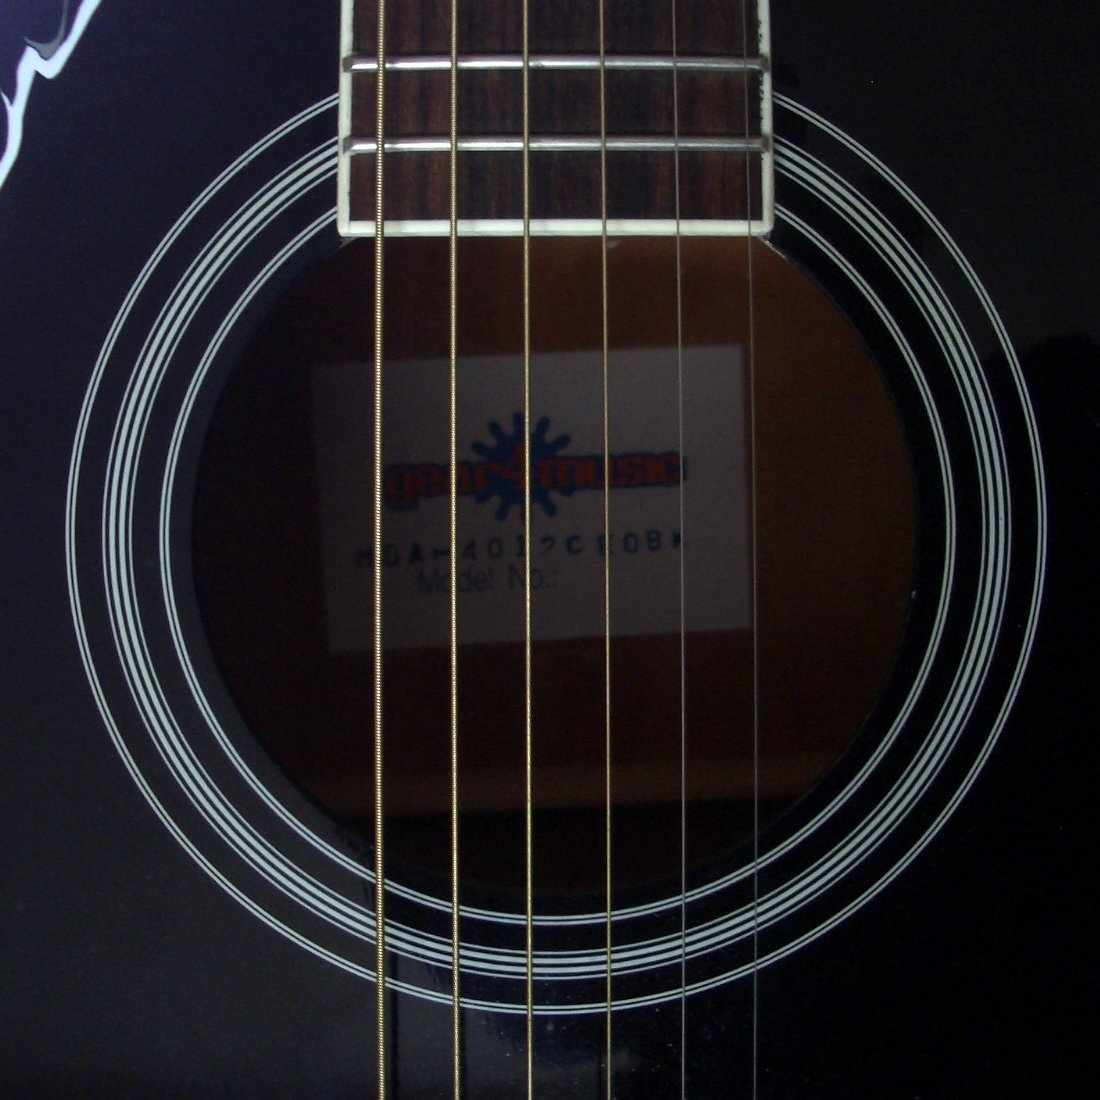
\includegraphics[width=0.95\textwidth]{circle.jpg}
  \begin{center}
    {\large ``Circle''}\par
    Foto di Howard Dickins\par
    \url{http://www.flickr.com/photos/dorkomatic/4551822855/}\par
    Licenza: Creative Commons Attribution 2.0\par
  \end{center}
\newpage

\section{Luoghi geometrici}\label{sect:luoghi_geometrici}

\begin{definizione}
Nel piano, si dice \emph{luogo geometrico} l'insieme di tutti e soli i punti del piano che verificano una proprietà, detta \emph{proprietà caratteristica} del luogo geometrico.
\end{definizione}
Ad esempio,
\begin{itemize*}
\item l'asse di un segmento è il luogo geometrico dei punti del piano equidistanti dagli estremi del segmento;
\item la bisettrice di un angolo è il luogo geometrico dei punti equidistanti dai lati dell'angolo.
\end{itemize*}
Se consideriamo la definizione ``costruttiva'' di asse di un segmento come retta perpendicolare al segmento stesso e passante per il suo punto medio, è possibile dimostrare che la nuova definizione di asse come luogo geometrico è ad essa equivalente.
Vale cioè il seguente
\begin{teorema}
Nel piano, il luogo geometrico dei punti equidistanti da due punti dati $A$ e $B$ è la retta $r$, perpendicolare al segmento $AB$ e passante per $M$, punto medio di $AB$.
\end{teorema}

\noindent\begin{minipage}{0.7\textwidth}\parindent15pt
Sia $r$ la retta perpendicolare ad $AB$ condotta da $M$, punto medio di $AB$. Dimostriamo che un generico punto $P\in r$ è equidistante da $A$ e $B$ e viceversa, un generico punto $Q$ tale che $QA\cong QB$ appartiene ad $r$.
~\\

\noindent Ipotesi: $r\perp AB$, $AM\cong MB$, $P\in r$.\tab Tesi: $PA\cong PB$.

\begin{proof}
Uniamo $P$ con $A$, $B$ ed $M$. Per ipotesi $PM \perp AB$, per cui, nel triangolo $PAB$, il segmento $PM$ è contemporaneamente altezza e mediana relative al lato $AB$; pertanto il triangolo $PAB$ è isoscele sulla base $AB$, da cui la tesi.
\end{proof}

\noindent Ipotesi: $QA\cong QB$ e $AM\cong MB$.\tab Tesi: $Q\in r$.

\begin{proof}
Uniamo $Q$ con $A$, $B$ ed $M$. Per ipotesi il triangolo $QAB$ è isoscele sulla base $AB$; inoltre il segmento $QM$ è la mediana relativa alla base del triangolo isoscele, per cui $QM$ è anche altezza. dunque la retta $QM$ coincide con la retta $r$, cioè l'asse di $AB$.
\end{proof}
\end{minipage}\hfil
\begin{minipage}{0.3\textwidth}
	\centering% Copyright (c) 2015 Daniele Masini - d.masini.it@gmail.com

\begin{tikzpicture}[scale=1,font=\small]
\usetikzlibrary{calc}

\begin{scope}

\coordinate (a) at (-1.3,0);
\coordinate (b) at (1.3,0);
\coordinate (m) at ($(a)!0.5!(b)$);
\coordinate (p) at (0,1.2);

\draw[red, fill=red!10] (-.4,0) -- (-.4,.4) --(0,.4) -- (m);

\draw[fill] (a) circle (1.2pt) node[left] {$A$};
\draw[fill] (b) circle (1.2pt) node[right] {$B$};
\draw[fill] (m) circle (1.2pt) node[above right] {$M$};
\draw (a) -- (b);

\draw[blue, thick,dashdotted] (0,1.8) node[black,right] {$r$} -- (0,-1);
\draw[fill] (p) circle (1.2pt) node[right] {$P$};
\draw[dashed] (a) -- (p) -- (b);

\end{scope}

\begin{scope}[yshift=-3.5cm]

\coordinate (a) at (-1.3,0);
\coordinate (b) at (1.3,0);
\coordinate (m) at ($(a)!0.5!(b)$);
\coordinate (p) at (0,1.2);
\coordinate (q) at (0.3,1.3);

%\draw[red, fill=red!10] (-.4,0) -- (-.4,.4) --(0,.4) -- (m);

\draw[fill] (a) circle (1.2pt) node[left] {$A$};
\draw[fill] (b) circle (1.2pt) node[right] {$B$};
\draw[fill] (m) circle (1.2pt) node[above right] {$M$};
\draw (a) -- (b);

\draw[blue, thick,dashdotted] (0,1.8) node[black,right] {$r$} -- (0,-1);
\draw[fill] (q) circle (1.2pt) node[right] {$Q$};
\draw[dashed, red] (a) -- (q) -- (b);
\draw[dashed, blue] (q) -- (m);

\end{scope}

\end{tikzpicture}

\end{minipage}\vspace{5pt}

Analogamente, se consideriamo la classica definizione di bisettrice di un angolo come la semiretta interna all'angolo stesso avente origine nel suo vertice e tale da dividerlo in due angoli congruenti, possiamo dimostrare che la nuova definizione di bisettrice come luogo geometrico è equivalente a quest'ultima.
Vale cioè il seguente teorema.
\begin{teorema}
La bisettrice di un angolo è il luogo geometrico dei punti del piano equidistanti dai lati dell'angolo.
\end{teorema}

Sia $r\widehat{V}s$ un angolo (di vertice $V$ e di lati $r$ ed $s$) e sia $b$ la sua bisettrice (semiretta di origine $V$ che divide l'angolo a metà).
Verifichiamo prima che un generico punto $P\in b$ è equidistante da $r$ e da $s$.
~\\

\noindent Ipotesi: $P\in b$, $PK\perp s$, $PH\perp r$, $K\widehat{V}P\cong P\widehat{V}H$.\tab Tesi: $PK\cong PH$.\vspace{10pt}

\noindent\begin{minipage}{0.65\textwidth}\parindent15pt
\begin{proof}
Tracciamo da $P$ le perpendicolari ai lati dell'angolo e chiamiamo $H\in r$ e $K\in s$ i piedi delle due perpendicolari. Osserviamo che i triangoli $VPH$ e $VPK$, rettangoli rispettivamente in $H$ e $K$, risultano congruenti perché hanno rispettivamente congruenti l'ipotenusa e un angolo acuto, per i criteri di congruenza sui triangoli rettangoli risultano congruenti. Pertanto i cateti $PH$ e $PK$, opposti a $V$, risultano congruenti, da cui la tesi ($P$ equidistante da $r$ e da $s$).
\end{proof}
\end{minipage}\hfil
\begin{minipage}{0.35\textwidth}
	\centering% (c) 2014 Daniele Masini - d.masini.it@gmail.com
\begin{tikzpicture}[scale=1,font=\small]
\usetikzlibrary{calc}

\begin{scope}
\pgfmathsetmacro{\aalpha}{-20};
\pgfmathsetmacro{\abeta}{40};
\pgfmathsetmacro{\agamma}{(\abeta+\aalpha)/2};

\coordinate (o) at (0,0);

\coordinate (p) at ({\agamma}:2);

\draw (o) node[left] {$V$} -- ++({\aalpha}:2.3) coordinate (a) node[right] {$s$};
\draw (o) -- ++({\abeta}:2.3) coordinate (b) node[right] {$r$};
\draw[blue, thick, dashdotted] (o) -- ++({\agamma}:2.5) coordinate (c) node[right,black] {$b$};
\draw[fill] (p) circle (1.2pt) node[above] {$P$};
\draw[dashed] (p) -- ($(o)!(p)!(b)$) coordinate (h);
\draw[fill] (h) circle (1.2pt) node[above] {$H$};
\draw[dashed] (p) -- ($(o)!(p)!(a)$) coordinate (k);
\draw[fill] (k) circle (1.2pt) node[below] {$K$};

%\draw[thick,gray] ([shift=({\aalpha}:.5)]o) arc [radius=.5, start angle={\aalpha}, end angle={\abeta}];
\draw[thick,red] ([shift=({\abeta}:.8)]o) arc [radius=.8, start angle={\abeta}, end angle={\agamma}];
\draw[thick,red] ([shift=({\agamma}:.7)]o) arc [radius=.7, start angle={\agamma}, end angle={\aalpha}];
\end{scope}

\end{tikzpicture}

\end{minipage}\vspace{5pt}

Ovviamente, un qualsiasi punto appartenente ad una delle due semirette $r$ o $s$ che non sia il vertice $V$ non può essere equidistante da $r$ e da $s$, mentre il punto $V$ lo è (ha distanza nulla da entrambe).

Verifichiamo ora che, se $Q$ è un generico punto interno all'angolo $r\widehat{V}s$, se $Q$ è equidistante da $r$ e da $s$, deve risultare $Q\in b$.
~\\

\noindent Ipotesi: $QT\perp s$, $QL\perp r$, $QL\cong QT$.\tab Tesi: $T\widehat{V}Q\cong Q\widehat{V}L$.\vspace{10pt}

\noindent\begin{minipage}{0.65\textwidth}\parindent15pt
\begin{proof}
Infatti, se tracciamo da $Q$ le perpendicolari alle semirette $r$ ed $s$ e chiamiamo $L\in r$ e $T\in s$ i piedi delle perpendicolari, per ipotesi risulta $QL\cong QT$. Se uniamo $Q$ con $V$, si vengono a formare due triangoli rettangoli $QLV$ e $QTV$ con l'ipotenusa $QV$ in comune ed una coppia di cateti congruenti. Tali triangoli risultano pertanto congruenti per il quarto criterio (più semplicemente per il criterio particolare dei triangoli rettangoli), e di conseguenza $L\widehat{V}Q\cong Q\widehat{V}T$, per cui la semiretta $VQ$ coincide con la bisettrice $b$.
\end{proof}
\end{minipage}\hfil
\begin{minipage}{0.35\textwidth}
	\centering\begin{tikzpicture}[scale=1,font=\small]
\usetikzlibrary{calc}

\begin{scope}
\pgfmathsetmacro{\aalpha}{-20};
\pgfmathsetmacro{\abeta}{40};
\pgfmathsetmacro{\agamma}{(\abeta+\aalpha)/2};

\coordinate (o) at (0,0);

\coordinate (p) at ({\agamma}:2);
\coordinate (q) at ({\agamma+7}:2);

\draw (o) node[left] {$V$} -- ++({\aalpha}:2.3) coordinate (a) node[right] {$s$};
\draw (o) -- ++({\abeta}:2.3) coordinate (b) node[right] {$r$};
\draw[blue, thick, dashdotted] (o) -- ++({\agamma}:2.5) coordinate (c) node[right,black] {$b$};
\draw[fill] (q) circle (1.2pt) node[above] {$Q$};
\draw[dashed, red] (q) -- ($(o)!(q)!(b)$) coordinate (h);
\draw[fill] (h) circle (1.2pt) node[above] {$L$};
\draw[dashed, red] (q) -- ($(o)!(q)!(a)$) coordinate (k);
\draw[fill] (k) circle (1.2pt) node[below] {$T$};
\draw[blue, dashed] (o) -- (q);

%\draw[thick,gray] ([shift=({\aalpha}:.5)]o) arc [radius=.5, start angle={\aalpha}, end angle={\abeta}];
%\draw[thick,red] ([shift=({\abeta}:.8)]o) arc [radius=.8, start angle={\abeta}, end angle={\agamma}];
%\draw[thick,red] ([shift=({\agamma}:.7)]o) arc [radius=.7, start angle={\agamma}, end angle={\aalpha}];
\end{scope}

\end{tikzpicture}

\end{minipage}\vspace{5pt}


\section{Circonferenza e cerchio: definizioni e prime proprietà}\label{sect:circonferenza_cerchio_def}

La definizione che ha dato Euclide di circonferenza fa riferimento ai luoghi geometrici: la circonferenza è il luogo geometrico dei punti del piano equidistanti da un punto del piano stesso, detto centro.
Intuitivamente, immaginiamo di fissare su di un piano un chiodo, di legare a questo chiodo una corda e di fissare all'altra estremità della corda una penna. Se facciamo ruotare la penna intorno al chiodo tenendo sempre in tensione la corda disegneremo una circonferenza.

\begin{definizione}
Assegnati nel piano un punto $C$ e un segmento $AB$, si chiama \emph{circonferenza} il luogo dei punti del piano che hanno distanza da $C$ congruente al segmento $AB$. Il punto $C$ viene detto \emph{centro} della circonferenza e la distanza dei punti della circonferenza dal centro è detta \emph{raggio} della circonferenza.
\end{definizione}

\osservazione Una circonferenza divide il piano in 3 insiemi:
\begin{itemize*}
\item l'insieme dei punti la cui distanza dal centro è minore del raggio. Questi punti si dicono \emph{interni} alla circonferenza.
\item l'insieme dei punti la cui distanza dal centro è uguale al raggio. Essi sono esattamente i punti della circonferenza.
\item l'insieme dei punti la cui distanza dal centro è maggiore del raggio. Questi punti si dicono \emph{esterni} alla circonferenza.
\end{itemize*}

Se consideriamo l'unione dell'insieme dei punti della circonferenza con l'insieme dei punti interni alla circonferenza otteniamo un cerchio.

\begin{definizione}
Chiamiamo \emph{cerchio} la figura formata dai punti di una circonferenza e dai punti interni ad essa.
\end{definizione}

Abbiamo definito la circonferenza come un insieme di punti tutti equidistanti dal centro. Viceversa osserviamo che il centro è l'unico punto del piano equidistante da tutti i punti della circonferenza. Per questo motivo possiamo affermare che una circonferenza è individuata esattamente dal suo centro e dal suo raggio o equivalentemente dal centro e da un suo punto.

\begin{definizione}
Un segmento che ha come estremi due punti distinti di una circonferenza è detto \emph{corda}. In particolare, una corda che contiene il centro della circonferenza viene definita \emph{diametro}.
\end{definizione}

I punti estremi di un diametro vengono detti \emph{diametralmente opposti}.
Ogni diametro è il doppio di un raggio e tutti i diametri della stessa circonferenza sono fra essi congruenti. Il centro della circonferenza è anche il punto medio di ciascun diametro.

Diamo ora alcune importanti proprietà delle corde.

\begin{teorema}
Il diametro è la corda di lunghezza massima.
\end{teorema}

\noindent\begin{minipage}{0.65\textwidth}\parindent15pt
\begin{proof}
Data una circonferenza di centro $O$ e raggio $r$, consideriamo una corda qualsiasi $AB$. Se essa passa per il centro $O$, coincide con il diametro e dunque $AB=2r$; altrimenti essa può essere considerata come la base di un triangolo isoscele $AOB$ avente come lati i due raggi $OA$ e $OB$. In tal caso per la disuguaglianza triangolare un lato di un triangolo è minore della somma degli altri due lati e dunque possiamo scrivere: $AB < OA + OB$ ovvero $AB < 2r$.
In conclusione, il diametro è maggiore di qualunque altra corda che non passa per il centro.
\end{proof}
\end{minipage}\hfil
\begin{minipage}{0.35\textwidth}
	\centering% Copyright (c) 2015 Daniele Masini - d.masini.it@gmail.com

\begin{tikzpicture}[scale=.9,font=\small]
\usetikzlibrary{calc}

\begin{scope}
\pgfmathsetmacro{\aalpha}{-20};
\pgfmathsetmacro{\abeta}{40};
\pgfmathsetmacro{\agamma}{(\abeta+\aalpha)/2};

\coordinate (o) at (0,0);

\coordinate (p) at ({\agamma}:2);
\coordinate (q) at ({\agamma+7}:2);

\draw (o) circle (2);
\draw[fill] (o) circle (1.2pt) node[right] {$O$};

\draw[dashed] (o) -- node[below, midway, sloped] {$r$} (80:2) coordinate (b);
\draw[dashed] (o) -- node[below, midway, sloped] {$r$} (180:2) coordinate (a);
\draw[fill] (a) circle (1.2pt) node[left] {$A$};
\draw[fill] (b) circle (1.2pt) node[above] {$B$};
\draw (a) -- (b);
\path (o) -- (40:2) coordinate (d2);
\path (o) -- (40:-2) coordinate (d1);
\draw[blue, dashed] (d1) -- node[black, shift={(0.8,0)}, below, sloped] {$d$} (d2);
\path (o) -- (130:2) coordinate (o1);
\path (o) -- (130:-1) coordinate (o2);
\coordinate (h) at (intersection of o--o1 and a--b);
\draw[red, dashdotted] (o1) -- (o2) node[black, left] {$a$};
\draw[fill] (h) circle (1.2pt) node[above] {$H$};


\end{scope}

\end{tikzpicture}

\end{minipage}

\begin{teorema}
L'asse di una corda qualsiasi passa per il centro della circonferenza.
\end{teorema}

\noindent Ipotesi: $A$ e $B$ due punti distinti appartenenti alla circonferenza, $a$ asse della corda $AB$.\tab Tesi: l'asse passa per il centro della circonferenza.

\begin{proof}
Facendo riferimento alla figura precedente, poiché $OA$ e $OB$ sono raggi della circonferenza, il triangolo $AOB$ è isoscele sulla base $AB$. Ricordiamo che l'asse relativo alla base di un triangolo isoscele contiene l'altezza (nella figura $OH$). Dunque $O$ appartiene all'asse $a$ di $AB$.
Se la corda $AB$ coincide con un diametro, $O$ ne è il punto medio; ma poiché l'asse di un segmento è la retta perpendicolare al segmento stesso nel suo punto medio, in ogni caso l'asse passa per il centro $O$ della circonferenza.
\end{proof}

\begin{teorema}
Un diametro passante per il punto medio di una corda è perpendicolare alla corda stessa.
\end{teorema}

\noindent\begin{minipage}{0.65\textwidth}\parindent15pt
\begin{proof}
Il diametro passa per ipotesi dal punto medio $H$ della corda $AB$ e per definizione da $O$, centro della circonferenza nonché vertice del triangolo isoscele $AOB$. Dunque $OH$ è mediana del triangolo $AOB$ relativamente alla base $AB$. Per il teorema sul triangolo isoscele, la mediana relativa alla base di un triangolo isoscele è anche altezza e quindi essa è perpendicolare alla corda $AB$.
\end{proof}
\end{minipage}\hfil
\begin{minipage}{0.35\textwidth}
	\centering\begin{tikzpicture}[scale=.75,font=\small]
\usetikzlibrary{calc}

\clip (-2.6,-2.6) rectangle (2.6,2.01);
\begin{scope}[rotate=180]
\pgfmathsetmacro{\aalpha}{-20};
\pgfmathsetmacro{\abeta}{40};
\pgfmathsetmacro{\agamma}{(\abeta+\aalpha)/2};

\coordinate (o) at (0,0);

\coordinate (p) at ({\agamma}:2);
\coordinate (q) at ({\agamma+7}:2);

\draw (o) circle (2);
\draw[fill] (o) circle (1.2pt) node[above] {$O$};

\draw[dashed] (o) -- node[above, midway, sloped] {$r$} (80:2) coordinate (b);
\draw[dashed] (o) -- node[above, midway, sloped] {$r$} (180:2) coordinate (a);
\draw[fill] (a) circle (1.2pt) node[right] {$A$};
\draw[fill] (b) circle (1.2pt) node[below] {$B$};
\draw (a) -- (b);
\path (o) -- (130:2) coordinate (o1);
\path (o) -- (130:-2) coordinate (o2);
\coordinate (h) at (intersection of o--o1 and a--b);
\draw[red, dashed] (o1) -- (o2);
\draw[fill] (h) circle (1.2pt) node[below] {$H$};


\end{scope}

\end{tikzpicture}

\end{minipage}

\begin{teorema}
In una circonferenza, corde congruenti hanno eguale distanza dal centro (e viceversa).
\end{teorema}

\noindent\begin{minipage}{0.65\textwidth}\parindent15pt
\noindent Ipotesi:
\begin{itemize*}
\item $AB\cong CD$ (corde congruenti);
\item $OH\perp AB$ ($OH$ distanza della corda $AB$ dal centro $O$);
\item $OK\perp CD$ ($OK$ distanza della corda $CD$ dal centro $O$).
\end{itemize*}
\noindent Tesi: $OH\cong OK$.

\begin{proof}
Consideriamo triangoli isosceli $AOB$ e $COD$; essi sono congruenti per il 3\textsuperscript{o} criterio di congruenza poiché per ipotesi le basi $AB$ e $CD$ sono congruenti e i lati $AO$, $OB$, $OC$ e $OD$ sono tutti raggi della circonferenza.
Di conseguenza anche le altezze $OH$ e $OK$ sono congruenti.
\end{proof}
\end{minipage}\hfil
\begin{minipage}{0.35\textwidth}
	\centering% Copyright (c) 2015 Daniele Masini - d.masini.it@gmail.com

\begin{tikzpicture}[scale=.9,font=\small]
\usetikzlibrary{calc}

\begin{scope}
\pgfmathsetmacro{\aalpha}{-20};
\pgfmathsetmacro{\abeta}{40};
\pgfmathsetmacro{\agamma}{(\abeta+\aalpha)/2};

\coordinate (o) at (0,0);

\draw (o) circle (2);
\draw[fill] (o) circle (1.2pt) node[below left] {$O$};

\draw[dashed] (o) -- (80:2) coordinate (b);
\draw[dashed] (o) -- (180:2) coordinate (a);
\draw[fill] (a) circle (1.2pt) node[left] {$A$};
\draw[fill] (b) circle (1.2pt) node[above] {$B$};
\path (o) -- (130:2) coordinate (o1);
\coordinate (h) at (intersection of o--o1 and a--b);
\begin{scope}[rotate=40]
\draw[red,fill=red!10] (h) rectangle ([shift={(0.3,-0.3)}]h);
\end{scope}
\draw[thick, orange] (a) -- (b);
\draw[fill] (h) circle (1.2pt) node[above] {$H$};
\draw[dashed, blue] (o) -- (h);

\draw[dashed] (o) -- (30:2) coordinate (c);
\draw[dashed] (o) -- (-70:2) coordinate (d);
\draw[fill] (c) circle (1.2pt) node[right] {$C$};
\draw[fill] (d) circle (1.2pt) node[below] {$D$};
\path (o) -- (-20:2) coordinate (o2);
\coordinate (k) at (intersection of o--o2 and c--d);
\begin{scope}[rotate=70]
\draw[red,fill=red!10] (k) rectangle ([shift={(-0.3,0.3)}]k);
\end{scope}
\draw[thick, orange] (c) -- (d);
\draw[fill] (k) circle (1.2pt) node[right] {$K$};
\draw[dashed, blue] (o) -- (k);

\end{scope}

\end{tikzpicture}

\end{minipage}\vspace{8pt}

\noindent Viceversa\vspace{5pt}

\noindent Ipotesi:
\begin{itemize*}
\item $OH\cong OK$ (le distanze delle corde $AB$ e $CD$ dal centro $O$ sono congruenti);
\item $OH\perp AB$ ($OH$ distanza della corda $AB$ dal centro $O$);
\item $OK\perp CD$ ($OK$ distanza della corda $CD$ dal centro $O$).
\end{itemize*}
\noindent Tesi: $AB\cong CD$.

\begin{proof}
Consideriamo i triangoli rettangoli $AOH$ e $DOK$. $AO\cong DO\cong r$ (raggio della circonferenza) e $OH\cong OK$ per ipotesi; per il criterio particolare dei triangoli rettangoli, i due triangoli sono congruenti e quindi $AH\cong DH$. Allo stesso modo possiamo dimostrare che i triangoli rettangoli $BOH$ e $COK$ sono congruenti, per cui $BH\cong CK$. Dunque $AB \cong AH + BH \cong DK + CK \cong CD$.
\end{proof}

\begin{teorema}
Fra due corde disuguali, è maggiore quella che ha distanza minore dal centro (e viceversa).
\end{teorema}

\noindent Ipotesi:
\begin{itemize*}
\item $AB>CD$ (corde disuguali),
\item $OH\perp AB$ ($OH$ distanza della corda $AB$ dal centro $O$),
\item $OK\perp CD$ ($OK$ distanza della corda $CD$ dal centro $O$).
\end{itemize*}
\noindent Tesi: $OH\cong OK$.\vspace{10pt}

\noindent\begin{minipage}{0.65\textwidth}\parindent15pt
\begin{proof}
A partire dal punto $A$ e allontanandosi dal punto $B$ si tracci la corda $AM$, consecutiva alla corda $AB$, in modo che $AM\cong CD$. Detta $OJ$ la distanza della corda $AM$ dal centro $O$, si ha che $OJ\perp AM$. Per il teorema precedente, essendo $CD$ e $AM$ corde congruenti, sarà $OJ\cong OK$; dunque basterà dimostrare che $OH < OJ$. Per ipotesi $AB > CD$, dunque $AB > AM$. Il senso di tale disuguaglianza vale anche per le rispettive metà dei segmenti $AB$ e $AM$, per cui $AH > AJ$ ($H$ è il punto medio di $AB$ e $J$ è il punto medio di $AM$ perché i triangoli $AOB$ e $AOM$ sono isosceli sulle basi $AB$ e $AM$, per cui $OH$ ed $OJ$, altezze relative alle basi, sono anche mediane).
Si congiunga $J$ con $H$ e si consideri il triangolo $HAJ$. A lato maggiore si oppone angolo maggiore (per le disuguaglianze tra gli elementi di un triangolo) per cui $H\widehat{J}A>A\widehat{H}J$; i rispettivi angoli complementari sono disuguali in verso opposto, quindi $H\widehat{J}O<O\widehat{H}J$. Relativamente al triangolo $HOJ$, poiché ad angolo minore si oppone lato minore (sempre per le disuguaglianze tra gli elementi di un triangolo, proprietà inversa della precedente), possiamo concludere che $OH < OJ$.
\end{proof}
\end{minipage}\hfil
\begin{minipage}{0.35\textwidth}
	\centering\begin{tikzpicture}[scale=1,font=\small]
\usetikzlibrary{calc}

\begin{scope}
\pgfmathsetmacro{\aalpha}{-20};
\pgfmathsetmacro{\abeta}{40};
\pgfmathsetmacro{\agamma}{(\abeta+\aalpha)/2};

\coordinate (o) at (0,0);

\draw (o) circle (2);
\draw[fill] (o) circle (1.2pt) node[below] {$O$};

\path (o) -- (80:2) coordinate (b);
\path (o) -- (180:2) coordinate (a);
\path (o) -- (130:2) coordinate (o1);
\coordinate (h) at (intersection of o--o1 and a--b);

\path (o) -- (10:2) coordinate (c);
\path (o) -- (-30:2) coordinate (d);
\path (o) -- (-10:2) coordinate (o2);
\coordinate (k) at (intersection of o--o2 and c--d);

\path (o) -- (220:2) coordinate (m);
\path (o) -- (200:2) coordinate (o3);
\coordinate (j) at (intersection of o--o3 and a--m);

\begin{scope}
\clip (o) -- (j) -- (h) -- cycle;
\draw[orange!70!black, fill=orange!10] (h) circle (0.4);
\draw[orange!70!black, fill=orange!10] (j) circle (0.4);
\end{scope}

\begin{scope}
\clip (a) -- (j) -- (h) -- cycle;
\draw[green!60!black, fill=green!10] (h) circle (0.4);
\draw[green!60!black, fill=green!10] (j) circle (0.4);
\end{scope}

\draw[dotted] (a) -- (o) -- (b);
\draw[dotted] (o) -- (m);

\draw[fill] (a) circle (1.2pt) node[left] {$A$};
\draw[fill] (b) circle (1.2pt) node[above] {$B$};
\begin{scope}[rotate=40]
\draw[red,fill=red!10] (h) rectangle ([shift={(0.3,-0.3)}]h);
\end{scope}
\draw[thick, blue] (a) -- (b);
\draw[fill] (h) circle (1.2pt) node[above] {$H$};
\draw[dashed] (o) -- (h);

\draw[fill] (c) circle (1.2pt) node[right] {$C$};
\draw[fill] (d) circle (1.2pt) node[below] {$D$};
\begin{scope}[rotate=-10]
\draw[red,fill=red!10] (k) rectangle ([shift={(-0.3,0.3)}]k);
\end{scope}
\draw[thick, red] (c) -- (d);
\draw[fill] (k) circle (1.2pt) node[right] {$K$};
\draw[dashed] (o) -- (k);

\draw[fill] (m) circle (1.2pt) node[below] {$M$};
\begin{scope}[rotate=200]
\draw[red,fill=red!10] (j) rectangle ([shift={(-0.3,0.3)}]j);
\end{scope}
\draw[red] (a) -- (m);
\draw[fill] (j) circle (1.2pt) node[left] {$J$};
\draw[dashed] (o) -- (j);

\draw (h) -- (j);


\end{scope}

\end{tikzpicture}

\end{minipage}\vspace{10pt}

\noindent Viceversa\vspace{10pt}

\noindent Ipotesi:
\begin{itemize*}
\item $OH<OK$ (distanze disuguali),
\item $OH\perp AB$ ($OH$ distanza della corda $AB$ dal centro $O$),
\item $OK\perp CD$ ($OK$ distanza della corda $CD$ dal centro $O$).
\end{itemize*}
\noindent Tesi: $AB>CD$.

\begin{proof}
Utilizziamo un metodo simile alla dimostrazione per assurdo, come abbiamo già fatto per la dimostrazione delle disuguaglianze tra gli elementi di un triangolo: esaminiamo tutti i casi possibili ed escludiamo i casi che contraddicono il teorema precedente ed il primo caso di questo teorema.
Sono possibili le seguenti relazioni tra le lunghezze delle corde $AB$ e $CD$:
\[\text{(1) }AB\cong CD\text{;}\qquad\qquad\text{(2) }AB < CD\text{;}\qquad\qquad\text{(3) }AB > CD\text{.}\]

Se fosse vera la relazione (1), per il teorema precedente risulterebbe $OH\cong OK$, contro l'ipotesi.

Se fosse vera la (2), per la prima parte di questo stesso teorema risulterebbe $OH > OK$, contro l'ipotesi.

Rimane solo la possibilità che valga la relazione (3), la quale non è in contraddizione con la prima parte del teorema e che anzi la conferma. Dunque la tesi è verificata.
\end{proof}

\pagebreak
Osservazioni:
\begin{itemize*}
\item Fissato un punto $P$, per esso passano infinite circonferenze.

Infatti, si consideri un qualunque altro punto $Q$: quest'ultimo può essere il centro di una circonferenza di raggio $QP$.

\item Per due punti fissati $A$ e $B$ passano infinite circonferenze.

Infatti, poiché tutti i punti dell'asse del segmento $AB$ sono equidistanti sia da $A$ che da $B$, essi possono essere centri di circonferenze passanti sia per $A$ che per $B$.
\end{itemize*}

\begin{definizione}
L'insieme di tutte le circonferenze passanti per due punti $A$ e $B$ è detto \emph{fascio di circonferenze}. Chiamiamo $A$ e $B$ \emph{punti base del fascio}, la retta per $A$ e $B$ \emph{asse radicale} e \emph{asse centrale} l'asse del segmento $AB$ che contiene tutti i centri delle circonferenze del fascio.
\end{definizione}

\begin{teorema}
Per tre punti distinti non allineati passa una ed una sola circonferenza.
\end{teorema}

\noindent\begin{minipage}{0.65\textwidth}\parindent15pt
\begin{proof}
Siano $A$, $B$ e $C$ tre punti non allineati e congiungiamo $A$ con $B$ e $B$ con $C$. Allora gli assi dei segmenti $AB$ e $BC$ si intersecheranno in un punto $O$. Per la proprietà degli assi il punto $O$, appartenendo a entrambi gli assi, è equidistante dai punti $A$, $B$ e $C$. Allora si può costruire una circonferenza con centro in $O$ e raggio $OA$. Questa circonferenza passa per $A$, $B$ e $C$, inoltre è unica perché è unico l'asse di un segmento e di conseguenza è unico il punto di intersezione tra i due assi.
\end{proof}
\end{minipage}\hfil
\begin{minipage}{0.35\textwidth}
	\centering% Copyright (c) 2015 Daniele Masini - d.masini.it@gmail.com

\begin{tikzpicture}[scale=.9,font=\small]
\usetikzlibrary{calc}

\begin{scope}
\pgfmathsetmacro{\aalpha}{-20};
\pgfmathsetmacro{\abeta}{40};
\pgfmathsetmacro{\agamma}{(\abeta+\aalpha)/2};

\coordinate (o) at (0,0);

\draw[dotted] (o) circle (2);
\draw[fill] (o) circle (1.2pt) node[right] {$O$};

\path (o) -- (80:2) coordinate (b);
\path (o) -- (140:2) coordinate (a);
\path (o) -- (110:2) coordinate (o1);
\coordinate (h) at (intersection of o--o1 and a--b);

\path (o) -- (10:2) coordinate (c);
\path (o) -- (45:2) coordinate (o2);
\coordinate (k) at (intersection of o--o2 and b--c);

\draw[fill] (a) circle (1.2pt) node[left] {$A$};
\draw[fill] (b) circle (1.2pt) node[above] {$B$};
\draw (a) -- (b);
%\draw[fill] (h) circle (1.2pt) node[above] {$H$};
\draw[dashdotted] ($(o)!-.5!(h)$) -- ($(o)!1.35!(h)$);

\draw[fill] (c) circle (1.2pt) node[right] {$C$};
\draw (b) -- (c);
%\draw[fill] (k) circle (1.2pt) node[right] {$K$};
\draw[dashdotted] ($(o)!-.5!(k)$) -- ($(o)!1.5!(k)$);

\end{scope}

\end{tikzpicture}

\end{minipage}

\osservazione
L'ipotesi che i punti siano non allineati è essenziale. Seguendo le linee della dimostrazione, i segmenti $AB$ e $BC$ sono consecutivi ma non adiacenti, cosa essenziale per affermare che i rispettivi assi non sono paralleli. Vale infatti anche la seguente proprietà:
\begin{teorema}
Dati tre punti distinti $A$, $B$ e $C$ appartenenti ad una stessa retta, non esiste alcuna circonferenza che passa per $A$, $B$ e $C$.
\end{teorema}

\begin{figure}[htb]
	\centering% Copyright (c) 2015 Daniele Masini - d.masini.it@gmail.com

\begin{tikzpicture}[scale=1,font=\small]
\usetikzlibrary{calc}

\begin{scope}

\draw (0,0) coordinate (a) -- (1,0) coordinate (b) -- (3,0) coordinate (c);

\draw[fill] (a) circle (1.2pt) node[above] {$A$};
\draw[fill] (b) circle (1.2pt) node[above] {$B$};
\draw[fill] (c) circle (1.2pt) node[above] {$C$};
\draw[dashdotted] (0.5,0.5) -- (0.5,-1.5);
\draw[dashdotted] (2,0.5) -- (2,-1.5);

\end{scope}

\end{tikzpicture}

\end{figure}

\begin{proof}
Verifichiamo che non esiste alcun punto del piano individuato da $A$, $B$ e $C$ che possa essere il centro di una tale circonferenza, cioè che sia equidistante dai tre punti.
Supponendo per assurdo che esista un tal punto $O$, questo, dovendo essere equidistante da $A$ e da $B$, dovrebbe appartenere all'asse del segmento $AB$ (luogo dei punti equidistanti dagli estremi) e, per ragioni analoghe, dovrebbe appartenere anche all'asse del segmento $BC$. Ma i punti $A$, $B$ e $C$ sono distinti per ipotesi, in particolare $A$ e $C$ non sono sovrapposti. Quindi, detto $M$ il punto medio di $AB$ ed $N$ il punto medio di $BC$, $M$ ed $N$ sono anch'essi distinti e pertanto gli assi dei segmenti $AB$, $BC$ non possono essere coincidenti; inoltre gli assi dei segmenti $AB$, $BC$ sono entrambi perpendicolari alla stessa retta che contiene i tre punti $A$, $B$, $C$ e quindi sono paralleli tra loro; essendo dunque rette parallele e distinte, i due assi non hanno punti in comune e pertanto non può esistere un punto $O$ che possa essere il centro della circonferenza passante per $A$, $B$ e $C$.
\end{proof}

\begin{corollario}
Tre punti qualsiasi appartenenti ad una circonferenza non sono allineati.
\end{corollario}

A conclusione di queste prime proprietà, possiamo enunciare il seguente
\begin{corollario}
Una circonferenza è univocamente determinata dal suo centro e dal suo raggio oppure da tre suoi punti.
\end{corollario}

Diamo ora la definizione di alcune parti del cerchio e della circonferenza. Ne esamineremo le proprietà in seguito.
\begin{definizione}
Data una circonferenza di centro $O$,
\begin{itemize*}
\item chiamiamo \emph{angolo al centro} un qualunque angolo con vertice in $O$;
\item l'intersezione della circonferenza con un angolo al centro $\gamma$ è detta \emph{arco} e diremo che l'angolo $\gamma$ insiste su tale arco;
\item i punti di intersezione della circonferenza con i lati dell'angolo si dicono \emph{estremi dell'arco};
\item un arco individuato da un angolo al centro piatto si chiama \emph{semicirconferenza}.
\end{itemize*}
\end{definizione}

\noindent\begin{minipage}{0.6\textwidth}\parindent15pt
Ogni coppia di punti distinti su una circonferenza individua due archi sulla medesima circonferenza. Infatti se consideriamo $A$ e $B$ ottenuti come nella definizione precedente questi punti individuano l'arco su cui insiste l'angolo $\gamma$ ma anche la restante parte di circonferenza che è pure un arco.
Congiungendo $A$ con $B$ il segmento $AB$ è una corda della circonferenza. Diremo che la corda $AB$ sottende l'arco $AB$ o viceversa che l'arco insiste sulla corda.
Se in particolare i punti $A$ e $B$ sono diametralmente opposti, essi individuano sulla circonferenza due archi che sono due semicirconferenze.
\end{minipage}\hfil
\begin{minipage}{0.4\textwidth}
	\centering% Copyright (c) 2015 Daniele Masini - d.masini.it@gmail.com

\begin{tikzpicture}[scale=1,font=\small]
\usetikzlibrary{calc}

\begin{scope}
\clip (-2.4,-2.01) rectangle (2.1,2.4);
\coordinate (o) at (0,0);

\draw (o) circle (2);
\draw[fill] (o) circle (1.2pt) node[below] {$O$};

\path (o) -- (100:2) coordinate (b);
\path (o) -- (170:2) coordinate (a);

\begin{scope}
\clip (a) -- (o) -- (b) -- cycle;
\draw[red, fill=red!10] (o) circle (0.4);
\end{scope}

\draw[thick] ($(a)!-.25!(o)$) -- (o) -- ($(b)!-.25!(o)$);

\draw[fill] (a) circle (1.2pt) node[shift={(-0.2,.-0.2)}] {$A$};
\draw[fill] (b) circle (1.2pt) node[shift={(0.2,0.2)}] {$B$};

\begin{scope}
\clip (a) -- (o) -- ++(b) -- ++($(a)-(o)$) -- cycle;
\draw[thick, blue] (o) circle (2) node[black, shift={(135:2.2)}, rotate=45] {arco};
\node at (-0.95,1) {angolo};
\node at (-0.95,0.6) {al centro};
\end{scope}

\end{scope}

\end{tikzpicture}

\end{minipage}

\begin{definizione}Dato un cerchio
\begin{itemize*}
\item si dice \emph{settore circolare} l'intersezione del cerchio con un suo angolo al centro: se l'angolo al centro è piatto di parla di \emph{semicerchio};
\item si chiama \emph{segmento circolare ad una base} la parte di cerchio limitata da una corda e da un arco che vi insiste; la corda viene detta \emph{base del segmento circolare};
\item la parte di cerchio limitata da due corde parallele è detta \emph{segmento circolare a due basi}, le due corde prendono il nome di \emph{basi del segmento circolare} e la loro distanza si dice \emph{altezza del segmento circolare}.
\end{itemize*}
\end{definizione}

Ogni corda divide il cerchio in due segmenti circolari ad una base. In particolare se la corda è un diametro otteniamo due semicerchi.
Un semicerchio, quindi, è sia un particolare settore circolare sia un particolare segmento circolare. \`E anche l'unico caso possibile di settore che sia anche segmento o viceversa.

\noindent\begin{minipage}{0.5\textwidth}\parindent15pt
Una coppia di corde parallele individua in un cerchio un segmento circolare a due basi e due segmenti circolari ad una base (se vogliamo considerare solo le tre parti non sovrapposte che hanno in comune al massimo una corda). Più in generale, date due corde parallele e distinte, queste individuano un segmento circolare a due basi e quattro segmenti circolari ad una base, ed il segmento a due basi è anche l'intersezione dei due segmenti ad una base ``sovrapposti''.
\end{minipage}\hfil
\begin{minipage}{0.5\textwidth}
	\centering\begin{tikzpicture}[scale=.8,font=\small]
\usetikzlibrary{calc}

\begin{scope}
%\clip (-2.01,-2.01) rectangle (2.01,2.01);
\coordinate (o) at (0,0);

\draw (o) circle (2);
\draw[fill] (o) circle (1.2pt) node[below] {$O$};

\coordinate (a) at (170:2);
\coordinate (b) at (100:2);
\coordinate (c) at (200:2);
\coordinate (d) at (280:2);

\coordinate (e) at (60:2);
\coordinate (f) at (40:2);
\coordinate (g) at (-50:2);
\coordinate (h) at (-30:2);

\begin{scope}
\clip (a) -- (o) -- ++(b) -- ++($(a)-(o)$) -- cycle;
\draw[thick, fill=blue!10] (o) circle (2);
\end{scope}

\draw[thick] (a) -- (o) -- (b);
\draw[thick, fill=blue!10] (c) -- (d) arc (280:200:2) -- cycle;
\draw[thick, fill=blue!10] (e) -- (g) arc (-50:-30:2) -- (h) -- (f) arc (40:60:2) -- cycle;

\coordinate (setc) at (-1,1);
\coordinate (setc_d) at (-1,2.3);
\node at (setc_d) {settore circolare};
\draw[->] ([shift={(-.5,-.3)}]setc_d) .. controls ([shift={(-.5,-.3)}]setc_d) and ([shift={(-.5,.5)}]setc) .. (setc);

\coordinate (segc) at (-1,-1.5);
\coordinate (segc_d) at (-1.2,-2.4);
\node at (segc_d) {segmento circolare};
\node at ([shift={(0,-.4)}]segc_d) {ad una base};
\draw[->] ([shift={(-.1,.3)}]segc_d) .. controls ([shift={(-.1,.3)}]segc_d) and ([shift={(-.2,-.2)}]segc) .. (segc);

\coordinate (segcc) at (1.5,-.8);
\coordinate (segcc_d) at (2,-2);
\node at (segcc_d) {segmento};
\node at ([shift={(0,-.36)}]segcc_d) {circolare};
\node at ([shift={(0,-.8)}]segcc_d) {a due basi};
\draw[->] ([shift={(0,.3)}]segcc_d) .. controls ([shift={(0,.4)}]segcc_d) and ([shift={(.2,-.2)}]segcc) .. (segcc);



\end{scope}

\end{tikzpicture}

\end{minipage}

\section{Posizioni relative fra rette e circonferenze}\label{sect:posizioni_rette_circonferenze}

Perché alcune strade a scorrimento veloce vengono chiamate ``tangenziali''?
Per rispondere a questa domanda dobbiamo definire le posizioni che può assumere una retta rispetto ad una circonferenza.
Consideriamo in uno stesso piano una circonferenza $C$ di centro $O$ e raggio $r$ e una retta generica $m$; la distanza $d$ fra il centro $O$ e la retta $m$ è definita dal segmento $OH$, che ha un estremo coincidente con il centro $O$ ed è perpendicolare in $H$ alla retta $m$ ($H$ è il piede della perpendicolare). Si possono distinguere i tre casi seguenti:\vspace{4pt}

\begin{enumeratea}

\noindent\begin{minipage}{0.6\textwidth}\parindent15pt
\item $d > r$ : la distanza del centro $O$ dalla retta è maggiore del raggio.\\
Il punto $H$ è esterno alla circonferenza così come ogni altro punto della retta $m$. La retta si dice allora \emph{esterna} alla circonferenza e non ha alcun punto in comune con essa, ovvero non vi sono punti di intersezione fra $C$ ed $m$.
\end{minipage}\hfil
\begin{minipage}{0.4\textwidth}
	\centering% Copyright (c) 2015 Daniele Masini - d.masini.it@gmail.com

\begin{tikzpicture}[scale=.7,font=\small]
\usetikzlibrary{calc}

\begin{scope}
\pgfmathsetmacro{\raggio}{1.7}
\clip (-\raggio-0.1,-\raggio-0.15) rectangle (2.9,\raggio+.4);
\coordinate (o) at (0,0);

\draw[thick] (o) circle (\raggio);
\draw[fill] (o) circle (1.2pt) node[left] {$O$};

\coordinate (r1) at (2.2,1.8);
\coordinate (r2) at (2.2,-1.8);

\coordinate (r) at (60:\raggio);

\draw[thick] (r1) node[right] {$m$} -- (r2);
\draw[blue] (o) -- node[black, above, midway, sloped] {$d$} ($(r1)!(o)!(r2)$) node[black, right] {$H$};
\draw[red] (o) -- node[black, above, midway, sloped] {$r$} (r);

\end{scope}

\end{tikzpicture}
\\\vspace{5pt}
\end{minipage}\vspace{4pt}

\noindent\begin{minipage}{0.6\textwidth}\parindent15pt
\item $d < r$ : la distanza del centro $O$ dalla retta è minore del raggio.\\
La retta $m$ interseca la circonferenza in due punti distinti $A$ e $B$; questi appartengono alla circonferenza e quindi $OA\cong OB\cong r$. Il segmento $AB$ appartiene alla retta e definisce anche la corda $AB$, i cui punti, tutti interni alla circonferenza, hanno una distanza dal centro minore del raggio; il punto di minore distanza è proprio $H$, che è anche il punto medio della corda $AB$. I punti della retta non appartenenti alla corda $AB$ sono esterni alla circonferenza e la loro distanza dal centro $O$ è maggiore del raggio.
La retta viene detta \emph{secante} alla circonferenza nei punti $A$ e $B$, che sono i punti di intersezione della retta con la circonferenza stessa.
\end{minipage}\hfil
\begin{minipage}{0.4\textwidth}
	\centering% (c) 2014 Daniele Masini - d.masini.it@gmail.com
\begin{tikzpicture}[scale=.7,font=\small]
\usetikzlibrary{calc,intersections}

\begin{scope}
\pgfmathsetmacro{\raggio}{1.7}
\clip (-\raggio-0.1,-\raggio-0.15) rectangle (2.9,\raggio+.5);
\coordinate (o) at (0,0);

\draw[name path=Circle1, thick] (o) circle (\raggio);
\draw[fill] (o) circle (1.2pt) node[left] {$O$};

\coordinate (r1) at (1,2);
\coordinate (r2) at (1,-1.8);

\draw[name path=Retta, thick] (r1) -- (r2);

\draw[thick] (r1) node[right] {$m$} -- (r2);
\draw[blue] (o) -- node[black, above, midway, sloped] {$d$} ($(r1)!(o)!(r2)$) node[black, right] {$H$};

\path [name intersections={of=Circle1 and Retta}] ;
\draw[fill] (intersection-1) coordinate (a) circle (1.2pt) node[right] {$A$};
\draw[fill] (intersection-2) coordinate (b) circle (1.2pt) node[right] {$B$};
\draw[red] (a) -- node[black, above, midway, sloped] {$r$} (o) -- node[black, below, midway, sloped] {$r$} (b);

\end{scope}

\end{tikzpicture}
\\\vspace{4pt}
	\centering% Copyright (c) 2015 Daniele Masini - d.masini.it@gmail.com

\begin{tikzpicture}[scale=.7,font=\small]
\usetikzlibrary{calc,intersections}

\begin{scope}
\pgfmathsetmacro{\raggio}{1.7}
\clip (-\raggio-0.1,-\raggio-0.15) rectangle (2.9,\raggio+.4);
\coordinate (o) at (0,0);

\draw[name path=Circle1, thick] (o) circle (\raggio);
\draw[fill] (o) circle (1.2pt) node[left] {$O$};

\coordinate (r1) at (\raggio,1.8);
\coordinate (r2) at (\raggio,-1.8);

\draw[name path=Retta, thick] (r1) -- (r2);

\draw[thick] (r1) node[right] {$m$} -- (r2);
\draw[blue] (o) -- node[black, above, midway, sloped] {$d=r$} ($(r1)!(o)!(r2)$) node[black, right] {$H$};

\end{scope}

\end{tikzpicture}
\\\vspace{4pt}
\end{minipage}\vspace{4pt}

\item $d = r$ : la distanza del centro $O$ dalla retta è pari al raggio.\\
Il punto $H$ appartiene alla circonferenza mentre ogni altro punto della retta $m$ è esterno alla circonferenza e ha una distanza dal centro $O$ maggiore del raggio. La retta viene detta \emph{tangente} alla circonferenza e $H$ è il punto di tangenza o di contatto.

\end{enumeratea}

\noindent\begin{minipage}{0.5\textwidth}\parindent15pt
Si noti che la retta tangente è perpendicolare al raggio nel punto di tangenza. Inoltre, l'unica retta perpendicolare al raggio nel punto di intersezione tra il raggio e la circonferenza è tangente.
Consideriamo una circonferenza $C$ di centro $O$ e raggio $r$ e una retta $m$ ad essa secante nei punti distinti $A$ e $B$. Sia $OH$ la distanza del centro $O$ dalla retta. 
Trasliamo la retta $m$ in modo da aumentare la sua distanza dal centro $O$ (vedi figura). All'aumentare della distanza $d = OH$, quella fra i punti $A$ e $B$ diminuisce; quando $OH = r$, i punti $A$ e $B$ coincidono nel punto di tangenza. Dunque la tangente è un caso particolare di secante avente due punti di intersezione coincidenti.
\end{minipage}\hfil
\begin{minipage}{0.5\textwidth}
	\centering\begin{tikzpicture}[scale=1,font=\small]
\usetikzlibrary{calc,intersections}

\begin{scope}
\pgfmathsetmacro{\raggio}{2}
\coordinate (o) at (0,0);

\draw[name path=Circle1] (o) circle (\raggio);
\draw[fill] (o) circle (1.2pt) node[left] {$O$};

\draw[red] (o) -- (\raggio,0);

\coordinate (r11) at (0.5,2.2);
\coordinate (r12) at (0.5,-2.2);
\draw[name path=Retta1] (r11) -- (r12);
\path [name intersections={of=Circle1 and Retta1}] ;
\draw[fill] (intersection-1) coordinate (a1) circle (1.2pt) node[shift={(.2,.2)}] {$A$};
\draw[fill] (intersection-2) coordinate (b1) circle (1.2pt) node[shift={(.2,-.2)}] {$B$};

\coordinate (r21) at (1,2.2);
\coordinate (r22) at (1,-2.2);
\draw[name path=Retta2] (r21) -- (r22);
\path [name intersections={of=Circle1 and Retta2}] ;
\draw[fill] (intersection-1) coordinate (a2) circle (1.2pt) node[shift={(.2,.2)}] {$A$};
\draw[fill] (intersection-2) coordinate (b2) circle (1.2pt) node[shift={(.2,-.2)}] {$B$};

\coordinate (r31) at (1.5,2.2);
\coordinate (r32) at (1.5,-2.2);
\draw[name path=Retta3] (r31) -- (r32);
\path [name intersections={of=Circle1 and Retta3}] ;
\draw[fill] (intersection-1) coordinate (a3) circle (1.2pt) node[shift={(.2,.2)}] {$A$};
\draw[fill] (intersection-2) coordinate (b3) circle (1.2pt) node[shift={(.2,-.2)}] {$B$};

\coordinate (r41) at (2,2.2);
\coordinate (r42) at (2,-2.2);
\draw[name path=Retta4] (r41) -- (r42);
\draw[fill] (2,0) coordinate (a4) circle (1.2pt) node[right] {$A\equiv B$};

\end{scope}

\end{tikzpicture}

\end{minipage}

\noindent\begin{minipage}{0.5\textwidth}\parindent15pt
Una più efficace ``visualizzazione'' di questo concetto è la seguente.
Consideriamo la stessa circonferenza e la stessa retta dell'esempio precedente. Ruotiamo la retta attorno al punto $B$ (vedi figura).
La distanza del punto $A$ dal punto $B$ diminuisce all'aumentare dell'angolo $O\widehat{B}A$ fra la retta e il raggio. Quando il punto $A$ coincide con il punto $B$, il raggio è perpendicolare alla retta e quest'ultima è tangente alla circonferenza in $B\equiv A$.
\end{minipage}\hfil
\begin{minipage}{0.5\textwidth}
	\centering% (c) 2014 Daniele Masini - d.masini.it@gmail.com
\begin{tikzpicture}[scale=1,font=\small]
\usetikzlibrary{calc,intersections}

\clip (-2.5, -2.5) rectangle (2.8,2.1);

\begin{scope}[rotate=30]
\pgfmathsetmacro{\raggio}{2}

\coordinate (o) at (0,0);

\draw[name path=Circle1] (o) circle (\raggio);
%\draw[fill] (o) circle (1.2pt) node[left] {$O$};

\coordinate (b) at (\raggio,0);
\draw [blue,name path=Retta1] (b) node[black,shift={(-.3,.05)}] {$B$} -- +(0:-4.5) -- +(0:4.2);
\path [name intersections={of=Circle1 and Retta1}] ;
\draw[fill] (intersection-2) coordinate (a1) circle (1.2pt) node[shift={(-.1,-.3)}] {$A$};
%\draw[fill] (intersection-2) coordinate (b1) circle (1.2pt) node[shift={(.2,-.2)}] {$B$};

\draw [blue,name path=Retta2] (b) -- +(15:-4.6) -- +(15:4.2);
\path [name intersections={of=Circle1 and Retta2}] ;
\draw[fill] (intersection-2) coordinate (a1) circle (1.2pt) node[shift={(-.1,-.3)}] {$A$};

\draw [blue,name path=Retta3] (b) -- +(30:-4.2) -- +(30:4.2);
\path [name intersections={of=Circle1 and Retta3}] ;
\draw[fill] (intersection-2) coordinate (a1) circle (1.2pt) node[shift={(0,-.2)}] {$A$};

\draw [blue,name path=Retta4] (b) -- +(45:-4.2) -- +(45:4.2);
\path [name intersections={of=Circle1 and Retta4}] ;
\draw[fill] (intersection-2) coordinate (a1) circle (1.2pt) node[shift={(.1,-.2)}] {$A$};

\draw [blue,name path=Retta5] (b) -- +(60:-4.2) -- +(60:4.2);
\path [name intersections={of=Circle1 and Retta5}] ;
\draw[fill] (intersection-1) coordinate (a1) circle (1.2pt) node[shift={(.2,-.2)}] {$A$};

\draw [blue,name path=Retta6] (b) -- +(75:-4.2) -- +(75:4.2);
\path [name intersections={of=Circle1 and Retta6}] ;
\draw[fill] (intersection-2) coordinate (a1) circle (1.2pt) node[shift={(.2,-.1)}] {$A$};

\draw [blue,name path=Retta7] (b) -- +(90:-4.2) -- +(90:4.2);

\end{scope}

\end{tikzpicture}

\end{minipage}

Il lettore dimostri per esercizio il seguente teorema (si suggerisce di ricorrere alla dimostrazione per assurdo).
\begin{teorema}
Se una retta è esterna ad una circonferenza, allora la sua distanza dal centro è maggiore del raggio, se è tangente la distanza dal centro è uguale al raggio e se è secante la distanza dal centro è minore del raggio.
\end{teorema}

Possiamo ora rispondere al quesito iniziale. Il termine ``tangenziale'' viene utilizzato per descrivere una strada a scorrimento veloce, realizzata in zone particolarmente urbanizzate, per permettere il transito degli autoveicoli senza dover entrare in contatto diretto con la circolazione urbana; ciò comporta evidenti benefici per la vivibilità dei centri cittadini. Possiamo immaginare il centro città racchiuso in un cerchio e la tangenziale come una retta di un certo spessore che è, appunto, tangente al cerchio.

\subsection{Posizioni reciproche di due circonferenze}

Descriviamo adesso le posizioni reciproche di due circonferenze.
\begin{definizione}
Due circonferenze si dicono:
\begin{itemize*}
\item \emph{esterne} se tutti i punti dell'una sono esterni all'altra;
\item \emph{secanti} quando hanno due punti in comune;
\item \emph{una interna all'altra} se i loro raggi sono diseguali e i punti della circonferenza di raggio minore sono tutti interni a quella di raggio maggiore;
\item \emph{tangenti} se hanno un solo punto in comune detto punto di tangenza; si possono inoltre distinguere fra: 
\begin{itemize*}
\item \emph{tangenti esternamente} se, ad eccezione del punto di tangenza, tutti i punti di una circonferenza sono esterni all'altra;
\item \emph{tangenti internamente} se i loro raggi sono diseguali e, ad eccezione del punto di tangenza, tutti i punti della circonferenza di raggio minore sono interni a quella di raggio maggiore.
\end{itemize*}
\end{itemize*}
\end{definizione}

Analizziamo in dettaglio i diversi casi; come esercizio lasciamo allo studente la dimostrazione rigorosa delle seguenti proprietà.

\begin{teorema}
Date due circonferenze esterne, la distanza fra i due centri è maggiore della somma dei raggi.
\end{teorema}

\begin{figure}[htb]
	\centering\begin{tikzpicture}[scale=.7,font=\small]
\usetikzlibrary{calc,intersections}

\begin{scope}
\pgfmathsetmacro{\raggioa}{2}
\pgfmathsetmacro{\raggiob}{1.3}
\coordinate (oa) at (0,0);
\coordinate (ob) at (4,0);

\draw[blue] (oa) -- (ob);

\draw[red] (oa) -- node[black, above, midway, sloped] {$r_1$} (45:\raggioa);
\draw[thick, name path=Circle1] (oa) circle (\raggioa);
\draw[fill] (oa) circle (1.2pt) node[below] {$O_1$};

\draw[red] (ob) -- node[black, above, midway, sloped] {$r_2$} +(135:\raggiob);
\draw[thick, name path=Circle2] (ob) circle (\raggiob);
\draw[fill] (ob) circle (1.2pt) node[below] {$O_2$};


\end{scope}

\end{tikzpicture}

\end{figure}

Abbiamo già dimostrato che per tre punti distinti non allineati passa una sola circonferenza, mentre per due punti passano infinite circonferenze. Di conseguenza due circonferenze distinte possono avere al massimo due punti in comune. \`E il caso delle circonferenze secanti. Se invece il numero di punti in comune è uno, allora ci riduciamo al caso delle circonferenze tangenti.

\begin{teorema}
Date due circonferenze secanti, la distanza fra i centri è maggiore della differenza dei raggi e minore della loro somma.
\end{teorema}

\begin{figure}[htb]
	\centering% Copyright (c) 2015 Daniele Masini - d.masini.it@gmail.com

\begin{tikzpicture}[scale=.7,font=\small]
\usetikzlibrary{calc,intersections}

\begin{scope}
\pgfmathsetmacro{\raggioa}{2}
\pgfmathsetmacro{\raggiob}{1.3}
\coordinate (oa) at (0,0);
\coordinate (ob) at (2.4,0);

\draw[blue] (oa) -- (ob);

\draw[red] (oa) -- node[black, above, midway, sloped] {$r_1$} (45:\raggioa);
\draw[thick, name path=Circle1] (oa) circle (\raggioa);
\draw[fill] (oa) circle (1.2pt) node[below] {$O_1$};

\draw[red] (ob) -- node[black, above, midway, sloped] {$r_2$} +(45:\raggiob);
\draw[thick, name path=Circle2] (ob) circle (\raggiob);
\draw[fill] (ob) circle (1.2pt) node[below] {$O_2$};

\path [name intersections={of=Circle1 and Circle2}] ;
\draw[fill] (intersection-1) coordinate (a) circle (1.5pt) node[shift={(.15,.3)}] {$A$};
\draw[fill] (intersection-2) coordinate (b) circle (1.5pt) node[shift={(.15,-.3)}] {$B$};
\draw[thick,green!40!black,dashdotted] ($(a)!-0.5!(b)$)--($(a)!1.5!(b)$);

\node at (8,0) {$\abs{r_1-r_2}<\overline{O_1O_2}<r_1+r_2$};

\end{scope}

\end{tikzpicture}

\end{figure}

La retta passante per i punti di intersezione viene detta \emph{asse radicale}.\label{def:asse_radicale}

Si dimostra che l'asse radicale è perpendicolare alla retta congiungente i centri.

\begin{teorema}
Data una circonferenza interna ad un'altra, la distanza fra i centri è minore della differenza fra i raggi.
\end{teorema}

\begin{figure}[!htb]
	\begin{center}
		\begin{minipage}{0.45\textwidth}
			\centering
			\begin{tikzpicture}[scale=.7,font=\small]
\usetikzlibrary{calc,intersections}

\begin{scope}
\pgfmathsetmacro{\raggioa}{2}
\pgfmathsetmacro{\raggiob}{1.3}
\coordinate (oa) at (0,0);
\coordinate (ob) at (.5,0);

\draw[blue] (oa) -- (ob);

\draw[red] (oa) -- node[black, above, midway, sloped, shift={(-.3,0)}] {$r_1$} (135:\raggioa);
\draw[thick, name path=Circle1] (oa) circle (\raggioa);
\draw[fill] (oa) circle (1.2pt) node[shift={(-.1,-.25)}] {$O_1$};

\draw[red] (ob) -- node[black, above, midway, sloped] {$r_2$} +(45:\raggiob);
\draw[thick, name path=Circle2] (ob) circle (\raggiob);
\draw[fill] (ob) circle (1.2pt) node[shift={(.1,-.25)}] {$O_2$};

\node at (0,-2.5) {circonferenza interna ad un'altra};

\node at (5.5,0) {$\overline{O_1O_2}<r_1-r_2$};

\end{scope}

\end{tikzpicture}

		\end{minipage}
		\hspace{0.03\textwidth}	
		\begin{minipage}{0.45\textwidth}
			\centering
			% Copyright (c) 2015 Daniele Masini - d.masini.it@gmail.com

\begin{tikzpicture}[scale=.7,font=\small]
\usetikzlibrary{calc,intersections}

\begin{scope}
\pgfmathsetmacro{\raggioa}{2}
\pgfmathsetmacro{\raggiob}{1.3}
\coordinate (o) at (0,0);

\begin{scope}
\draw[fill=yellow!15] (o) circle (\raggioa);
\draw[fill=white] (o) circle (\raggiob);
\end{scope}


\draw[red] (o) -- node[black, above, midway, sloped, shift={(-0.4,0)}] {$r_1$} (135:\raggioa);
\draw[thick, name path=Circle1] (o) circle (\raggioa);
\draw[fill] (o) circle (1.2pt) node[below] {$O$};

\draw[red] (o) -- node[black, above, midway, sloped] {$r_2$} +(45:\raggiob);
\draw[thick, name path=Circle2] (o) circle (\raggiob);

\node at (0,2.6) {$O_1\equiv O_2\equiv O$};
\node at (0,-2.6) {circonferenze concentriche};

\end{scope}

\end{tikzpicture}

		\end{minipage}
	\end{center}
\end{figure}

Un caso particolare di circonferenze una interna all'altra è rappresentato dalle \emph{circonferenze concentriche}, i cui centri coincidono. La zona di piano delimitata dalle due circonferenze è detta \emph{corona circolare}.

\begin{teorema}
Date due circonferenze tangenti esternamente in un punto $T$, la distanza fra i centri è uguale alla somma dei raggi. La retta tangente passante per $T$ è comune alle due circonferenze ed è perpendicolare alla retta congiungente i due centri.
\end{teorema}

\begin{figure}[htb]
	\centering% (c) 2014 Daniele Masini - d.masini.it@gmail.com
\begin{tikzpicture}[scale=.7,font=\small]
\usetikzlibrary{calc,intersections}

\begin{scope}
\pgfmathsetmacro{\raggioa}{2}
\pgfmathsetmacro{\raggiob}{1.3}
\coordinate (oa) at (0,0);
\coordinate (ob) at (3.3,0);

\draw[blue] (oa) -- (ob);
\draw[green!70!black, dashed] (2,-2) -- (2,2) node[black, right] {$t$};

\draw[red] (oa) -- node[black, above, midway, sloped] {$r_1$} (45:\raggioa);
\draw[thick, name path=Circle1] (oa) circle (\raggioa);
\draw[fill] (oa) circle (1.2pt) node[below] {$O_1$};

\draw[red] (ob) -- node[black, above, midway, sloped] {$r_2$} +(135:\raggiob);
\draw[thick, name path=Circle2] (ob) circle (\raggiob);
\draw[fill] (ob) circle (1.2pt) node[below] {$O_2$};

\draw[fill] (2,0) circle (1.5pt) node[shift={(-.2,-.25)}] {$T$};

\node at (1.2,2.6) {$\overline{O_1O_2}=r_1+r_2$};

\node at (1.2,-2.6) {circonferenze tangenti esternamente};

\end{scope}


\begin{scope}[xshift=10cm]
\pgfmathsetmacro{\raggioa}{2}
\pgfmathsetmacro{\raggiob}{1.3}
\coordinate (oa) at (0,0);
\coordinate (ob) at (0.7,0);

\draw[blue] (oa) -- (ob);
\draw[green!70!black, dashed] (2,-2) -- (2,2) node[black, right] {$t$};

\draw[red] (oa) -- node[black, above, midway, sloped, shift={(-.2,0)}] {$r_1$} (135:\raggioa);
\draw[thick, name path=Circle1] (oa) circle (\raggioa);
\draw[fill] (oa) circle (1.2pt) node[below] {$O_1$};

\draw[red] (ob) -- node[black, above, midway, sloped] {$r_2$} +(45:\raggiob);
\draw[thick, name path=Circle2] (ob) circle (\raggiob);
\draw[fill] (ob) circle (1.2pt) node[below] {$O_2$};

\draw[fill] (2,0) circle (1.5pt) node[right] {$T$};

\node at (0.2,2.6) {$\overline{O_1O_2}=\abs{r_1-r_2}$};

\node at (0.2,-2.6) {circonferenze tangenti internamente};

\end{scope}

\end{tikzpicture}

\end{figure}

\begin{teorema}
Date due circonferenze tangenti internamente, la distanza fra i centri è pari alla differenza dei raggi.
\end{teorema}


Anche per le circonferenze si può affermare che nel caso siano tangenti lo sono in due punti coincidenti; infatti se prendiamo due circonferenze secanti e man mano allontaniamo i loro centri, osserviamo che i due punti di intersezione si avvicinano sempre più fino a sovrapporsi nel momento in cui la distanza fra i loro centri è pari alla somma dei raggi.

\begin{figure}[htb]
	\centering\begin{tikzpicture}[scale=.6,font=\small]
\usetikzlibrary{calc,intersections}

\begin{scope}
\pgfmathsetmacro{\raggioa}{2}
\pgfmathsetmacro{\raggiob}{1.3}
\coordinate (oa) at (0,0);
\coordinate (ob) at (2,0);

\draw[name path=Circle1] (oa) circle (\raggioa);
\draw[name path=Circle2] (ob) circle (\raggiob);

\path [name intersections={of=Circle1 and Circle2}] ;
\draw[fill] (intersection-1) coordinate (a) circle (1.5pt) node[shift={(0,.3)}] {$A$};
\draw[fill] (intersection-2) coordinate (b) circle (1.5pt) node[shift={(0,-.3)}] {$B$};

\end{scope}

\begin{scope}[xshift=7cm]
\pgfmathsetmacro{\raggioa}{2}
\pgfmathsetmacro{\raggiob}{1.3}
\coordinate (oa) at (0,0);
\coordinate (ob) at (2.8,0);

\draw[name path=Circle1] (oa) circle (\raggioa);
\draw[name path=Circle2] (ob) circle (\raggiob);

\path [name intersections={of=Circle1 and Circle2}] ;
\draw[fill] (intersection-1) coordinate (a) circle (1.5pt) node[shift={(0,.3)}] {$A$};
\draw[fill] (intersection-2) coordinate (b) circle (1.5pt) node[shift={(0,-.3)}] {$B$};

\end{scope}


\begin{scope}[xshift=14.5cm]
\pgfmathsetmacro{\raggioa}{2}
\pgfmathsetmacro{\raggiob}{1.3}
\coordinate (oa) at (0,0);
\coordinate (ob) at (3.3,0);

\draw[name path=Circle1] (oa) circle (\raggioa);
\draw[name path=Circle2] (ob) circle (\raggiob);

\draw[fill] (2,0) coordinate (a) circle (1.5pt) node[right] {$A\equiv B$};

\end{scope}


\end{tikzpicture}

\end{figure}

Se esaminiamo le varie posizioni reciproche nel caso di due circonferenze congruenti ($r_1 = r_2 = r$), tenendo conto anche del fatto banale che in tal caso $\abs{r_1 - r_2} = 0$ e $r_1 + r_2 = 2r$, scompaiono le ``distinte'' possibilità che esse siano concentriche, interne e tangenti internamente, ma compare la possibilità che siano coincidenti, cioè perfettamente sovrapposte.
Lasciamo al lettore la ``rivisitazione'' dei casi precedentemente analizzati nell'ipotesi che le due circonferenze siano congruenti.

\section{Angoli nelle circonferenze}\label{sect:angoli_circonferenze}

\noindent\begin{minipage}{0.6\textwidth}\parindent15pt
Ricordiamo che abbiamo definito \emph{angolo al centro} di una circonferenza di centro $O$ e raggio $r$ un qualsiasi angolo avente come vertice il centro $O$.
Tracciato un angolo al centro, i suoi lati intersecano la circonferenza in due punti $P$ e $Q$ e di conseguenza l'angolo contiene l'arco $PQ$; si dice che l'angolo al centro $P\widehat{O}Q$ insiste sull'arco $PQ$ o sottende l'arco $PQ$.
Si noti che tracciate due semirette uscenti dal centro $O$, si vengono a formare due angoli al centro esplementari, ovvero la cui somma è un angolo giro, a cui corrispondono due distinti archi complementari $PQ$, la cui somma è il perimetro della circonferenza. 
I due angoli sono uno convesso e uno concavo, tranne il caso particolare in cui essi sono entrambi piatti, con le due semirette opposte. In tal caso, anche i relativi archi sono congruenti e ognuno ha misura pari al semiperimetro della circonferenza.
\end{minipage}\hfil
\begin{minipage}{0.4\textwidth}
	\centering% Copyright (c) 2015 Daniele Masini - d.masini.it@gmail.com

\begin{tikzpicture}[scale=1,font=\small]
\usetikzlibrary{calc}

\begin{scope}
\clip (-2.4,-2.01) rectangle (2.1,2.4);
\coordinate (o) at (0,0);

\draw (o) circle (2);

\path (o) -- (100:2) coordinate (b);
\path (o) -- (170:2) coordinate (a);

\begin{scope}
\clip (a) -- (o) -- (b) -- cycle;
\draw[red, fill=red!10] (o) circle (0.4);
\end{scope}

\begin{scope}
\clip (a) -- (o) -- ++(b) -- ++($(a)-(o)$) -- cycle;
\draw[thick, green!70!black, fill=green!05] (o) circle (2);
\draw[thick, green!55!black, fill=green!15] (o) circle (0.5);
\end{scope}

%\draw[blue] ($(a)!-.25!(o)$) -- (o) -- ++($(b)!-.25!(o)$) -- (2.25,2.25) -- (2.25,-2.25) -- (-2.25,-2.25) -- cycle;

\begin{scope}
\clip ($(a)!-.25!(o)$) -- (o) -- ++($(b)!-.25!(o)$) -- (2.25,2.25) -- (2.25,-2.25) -- (-2.25,-2.25) -- cycle;
\draw[thick, blue, fill=blue!05] (o) circle (2);
\draw[thick, blue!75!black, fill=blue!15] (o) circle (0.5);
\end{scope}

\draw[thick] ($(a)!-.25!(o)$) -- (o) -- ($(b)!-.25!(o)$);

\draw[fill] (a) circle (1.2pt) node[shift={(-0.2,.-0.2)}] {$P$};
\draw[fill] (b) circle (1.2pt) node[shift={(0.2,0.2)}] {$Q$};
\draw[fill] (o) circle (1.2pt) node[below] {$O$};


\end{scope}

\end{tikzpicture}

\end{minipage}

Diamo ora la seguente
\begin{definizione}
Data una circonferenza, si definisce \emph{angolo alla circonferenza} qualsiasi angolo avente il vertice sulla circonferenza e i cui lati siano secanti o tangenti alla circonferenza stessa. 
\end{definizione}
In base alla definizione si possono distinguere tre casi:
\begin{itemize*}
\item i lati dell'angolo sono entrambi secanti alla circonferenza;
\item un lato è secante e l'altro tangente;
\item ambedue i lati sono tangenti.
\end{itemize*}

Anche gli angoli alla circonferenza insistono su archi di circonferenza. Questi appartengono all'angolo stesso e sono delimitati dai punti di tangenza o di intersezione fra i lati dell'angolo e la circonferenza. Nella figura~\ref{fig:ang_circonf} gli angoli alla circonferenza sono segnati in rosso ed i rispettivi archi sono più marcati. Sono invece stati evidenziati in blu i corrispondenti angoli al centro, come segue dalla seguente definizione.

\begin{definizione}
Un angolo al centro ed un angolo alla circonferenza si dicono \emph{corrispondenti} se insistono sullo stesso arco.
\end{definizione}

\begin{figure}[htb]\label{fig:ang_circonf}
	\centering% Copyright (c) 2015 Daniele Masini - d.masini.it@gmail.com

\begin{tikzpicture}[scale=0.75,font=\small]
\usetikzlibrary{calc}

\begin{scope}
\clip (-3.4,-3.65) rectangle (3.4,2.5);
\coordinate (o) at (0,0);

\draw[very thin] (o) circle (2);

\path (o) -- (100:2) coordinate (b);
\path (o) -- (170:2) coordinate (a);
\path (o) -- (320:2) coordinate (c);

\begin{scope}
\clip (a) -- (o) -- (b) -- cycle;
\draw[blue, fill=blue!10] (o) circle (0.4);
\end{scope}

\begin{scope}
\clip ($(a)!-.25!(c)$) -- (c) -- ($(b)!-.25!(c)$) -- cycle;
\draw[thick] (o) circle (2);
\draw[red, fill=red!15] (c) circle (0.5);
\end{scope}

\draw[blue] ($(a)!-.25!(o)$) -- (o) -- ($(b)!-.25!(o)$);
\draw[thick, red] ($(a)!-.15!(c)$) -- (c) -- ($(b)!-.15!(c)$);

\draw[fill] (a) circle (1.2pt) node[shift={(-0.2,.-0.2)}] {$P$};
\draw[fill] (b) circle (1.2pt) node[shift={(0.2,0.2)}] {$Q$};
\draw[fill] (c) circle (1.2pt) node[shift={(0.2,-0.2)}] {$V$};
\draw[fill] (o) circle (1.2pt) node[below] {$O$};

\node at (0,-2.4) {L'angolo al centro $P\widehat{O}Q$};
\node at (0,-2.95) {corrisponde all'angolo};
\node at (0,-3.4) {alla circonferenza $P\widehat{V}Q$};

\end{scope}


\begin{scope}[xshift=6cm]
\clip (-3.4,-3.65) rectangle (3.4,2.5);
%\clip (-2.4,-2.1) rectangle (2.1,2.5);
\coordinate (o) at (0,0);

\path (o) -- (100:2) coordinate (b);
\path (o) -- (170:2) coordinate (a);
\path (b) -- +(10:2) coordinate (d);

\begin{scope}
\clip (a) -- (o) -- (b) -- (2.25,2.25) -- (2.25,-2.25) -- (-2.25,-2.25) -- cycle;
\draw[blue, fill=blue!10] (o) circle (0.4);
\end{scope}

\begin{scope}
\clip ($(a)!-.25!(b)$) -- (b) -- (d) -- (2.25,2.25) -- (2.25,-2.25) -- (-2.25,-2.25) -- cycle;
\draw[thick] (o) circle (2);
\draw[red, fill=red!15] (b) circle (0.5);
\end{scope}

\begin{scope}[rotate=10]
\draw[green!60!black, fill=green!10] (b) rectangle ([shift={(0.3,0.3)}]b);
\end{scope}

\draw[very thin] (o) circle (2);

\draw[blue] ($(a)!-.25!(o)$) -- (o) -- ($(b)!-.25!(o)$);
\draw[thick, red] ($(a)!-.25!(b)$) -- (b) -- (d);

\draw[fill] (a) circle (1.2pt) node[shift={(-0.2,0.2)}] {$P$};
\draw[fill] (b) circle (1.2pt) node[shift={(-0.6,0.2)}] {$V\equiv Q$};
\draw[fill] (o) circle (1.2pt) node[shift={(-0.25,0.25)}] {$O$};
\draw[fill] ($(b)!0.8!(d)$) circle (1.2pt) node[shift={(0.2,-0.2)}] {$T$};

\node at (0,-2.4) {L'angolo al centro $P\widehat{O}Q$};
\node at (0,-2.95) {corrisponde all'angolo};
\node at (0,-3.4) {alla circonferenza $P\widehat{V}T$};
\end{scope}


\begin{scope}[xshift=12cm]
\clip (-3.4,-3.65) rectangle (3.4,2.5);
%\clip (-3.1,-2.1) rectangle (2.1,2.5);
\coordinate (o) at (0,0);

\path (o) -- (100:2) coordinate (b);
\path (b) -- +(10:2) coordinate (d);
\path (b) -- +(190:2) coordinate (e);

\draw[blue, fill=blue!10] (o) circle (0.5);

\begin{scope}
\clip (e) -- (b) -- (d) -- (2.25,2.25) -- (2.25,-2.25) -- (-2.25,-2.25) -- cycle;
\draw[thick] (o) circle (2);
\draw[red, fill=red!15] (b) circle (0.5);
\end{scope}

\begin{scope}[rotate=10]
\draw[green!60!black, fill=green!10] (b) rectangle ([shift={(0.3,0.3)}]b);
\end{scope}

\draw[very thin] (o) circle (2);

\draw[blue] (o) -- ($(b)!-.25!(o)$);
\draw[thick, red] (e) -- (b) -- (d);

\draw[fill] (b) circle (1.2pt) node[shift={(-0.9,0.2)}] {$V\equiv Q\equiv P$};
\draw[fill] (o) circle (1.2pt) node[below] {$O$};

\node at (0,-2.45) {L'angolo (giro) al centro di vertice $O$};
\node at (0,-2.95) {corrisponde all'angolo (piatto)};
\node at (0,-3.45) {alla circonferenza di vertice $V$};

\end{scope}


\end{tikzpicture}

	\caption{Angoli alla circonferenza e corrispondenti angoli al centro}
\end{figure}

\begin{teorema}
L'angolo alla circonferenza è la metà del corrispondente angolo al centro.
\end{teorema}

\noindent Ipotesi:\tab $\alpha$ angolo alla circonferenza che insiste sull'arco $PQ$;\\
\tab\tab $\beta$ angolo al centro corrispondente ad $\alpha$.\vspace{4pt}\\
Tesi:\tab $\beta = 2\alpha$.

% figura

\begin{proof}
Distinguiamo tre casi:
\begin{enumerate*}
\item Un lato dell'angolo alla circonferenza passa per il centro e dunque si sovrappone al diametro.\\
Abbiamo due possibilità:
\begin{enumerate*}
\noindent\begin{minipage}{0.6\textwidth}\parindent15pt
\item L'altro lato è secante alla circonferenza.\\
Con riferimento alla figura a fianco, il triangolo $OVQ$ è isoscele sulla base $VQ$, in quanto i lati $OV$ e $OQ$ sono due raggi della circonferenza; ne segue che gli angoli alla base sono congruenti e dunque $O\widehat{Q}V\cong \alpha$. L'angolo al centro $P\widehat{O}Q\equiv \beta$ giace sul prolungamento del lato $OV$ e dunque è un angolo esterno al triangolo $OVQ$. Per il teorema degli angoli esterni ad un triangolo, possiamo affermare che $\beta$ è uguale alla somma degli angoli interni non adiacenti e quindi $\beta = \alpha + \alpha = 2\alpha$.
\end{minipage}\hfil
\noindent\hspace{-20pt}\begin{minipage}{0.4\textwidth}
	\centering% Copyright (c) 2015 Daniele Masini - d.masini.it@gmail.com

\begin{tikzpicture}[scale=0.75,font=\small]
\usetikzlibrary{calc}

\begin{scope}
\clip (-2.05,-2.05) rectangle (2.4,2.05);
\coordinate (o) at (0,0);

\draw[very thin] (o) circle (2);

\path (o) -- (0:2) coordinate (q);
\path (o) -- (315:2) coordinate (p);
\path (o) -- (135:2) coordinate (v);

\begin{scope}
\clip (p) -- (o) -- (q) -- cycle;
\draw[blue, fill=blue!10] (o) circle (0.5);
\draw[blue] (o) circle (0.4);
\node at ([shift={(335:0.8)}]o) {$\beta$};
\end{scope}

\begin{scope}
\clip ($(p)!-.15!(v)$) -- (v) -- ($(q)!-.15!(v)$) -- cycle;
\draw[thick] (o) circle (2);
\draw[red, fill=red!15] (v) circle (0.6);
\node at ([shift={(326:1)}]v) {$\alpha$};
\end{scope}

\draw[blue] ($(p)!-.2!(o)$) -- (o) -- ($(q)!-.2!(o)$);
\draw[red] ($(p)!-.15!(v)$) -- (v) -- ($(q)!-.15!(v)$);

\draw[fill] (p) circle (1.2pt) node[shift={(0,-0.3)}] {$P$};
\draw[fill] (q) circle (1.2pt) node[shift={(0.2,0.2)}] {$Q$};
\draw[fill] (v) circle (1.2pt) node[shift={(-0.2,0.2)}] {$V$};
\draw[fill] (o) circle (1.2pt) node[below] {$O$};
\end{scope}

\end{tikzpicture}

\end{minipage}
\noindent\begin{minipage}{0.6\textwidth}\parindent15pt
\item L'altro lato è tangente alla circonferenza.\\
In questo caso un lato coincide sempre con il diametro e l'altro è tangente alla circonferenza nel punto $V\equiv Q$; poiché le rette tangenti alla circonferenza sono sempre ortogonali al raggio nel punto di tangenza, i due lati sono perpendicolari. Di conseguenza l'angolo $\alpha$ è un angolo retto e il corrispondente angolo al centro $\beta$ è un angolo piatto, per cui $\beta = 2\alpha$.
\end{minipage}\hfil
\noindent\hspace{-20pt}\begin{minipage}{0.4\textwidth}
	\centering\begin{tikzpicture}[scale=0.75,font=\small]
\usetikzlibrary{calc}

\begin{scope}
\clip (-2.7,-2.05) rectangle (2.1,2.8);
\coordinate (o) at (0,0);

\path (o) -- (135:2) coordinate (q);
\path (o) -- (315:2) coordinate (p);
\path (o) -- (135:2) coordinate (v);
\path (v) -- +(45:2.1) coordinate (t);

\begin{scope}
\clip (p) -- (o) -- (q) -- (0,2.9) -- (2.1,2.1) -- (2.1,-2.1) -- cycle;
\draw[blue, fill=blue!10] (o) circle (0.5);
\draw[blue] (o) circle (0.4);
\node at ([shift={(45:0.8)}]o) {$\beta$};
\end{scope}

\begin{scope}
\clip (p) -- (v) -- (t) -- (2.1,2.1) -- (2.1,-2.1) -- cycle;
\draw[thick] (o) circle (2);
\draw[red, fill=red!15] (v) circle (0.5);
\node at ([shift={(0:0.7)}]v) {$\alpha$};
\end{scope}

\draw[very thin] (o) circle (2);

\draw[blue] ($(p)!-.2!(o)$) -- (o) -- ($(q)!-.1!(o)$);
\draw[red] ($(p)!-.15!(v)$) -- (v) -- (t);

\draw[fill] (p) circle (1.2pt) node[shift={(0,-0.3)}] {$P$};
\draw[fill] (v) circle (1.2pt) node[shift={(-0.45,0.3)}] {$V\equiv Q$};
\draw[fill] (o) circle (1.2pt) node[shift={(-0.2,-0.2)}] {$O$};
\end{scope}

\end{tikzpicture}

\end{minipage}
\end{enumerate*}

\item Il centro $O$ è interno all'angolo alla circonferenza.\\
Anche in questo caso abbiamo due possibilità:
\begin{enumerate*}
\noindent\begin{minipage}{0.6\textwidth}\parindent15pt
\item I lati dell'angolo alla circonferenza sono entrambi secanti.\\
Si conduca dal vertice $V$ dell'angolo alla circonferenza $P\widehat{V}Q$ il diametro $VT$; si ottengono in tal modo due angoli alla circonferenza $P\widehat{V}T$ e $T\widehat{V}Q$ la cui somma è proprio l'angolo $P\widehat{V}Q$. Tali angoli hanno il lato comune il lato $VT$ coincidente con il diametro e dunque, essendo $P\widehat{O}T$ e $T\widehat{O}Q$ i rispettivi angoli al centro, possiamo applicare ad ognuno di essi il risultato dimostrato al punto 1: $P\widehat{O}T=2P\widehat{V}T$ e $T\widehat{O}Q=2T\widehat{V}Q$.
Ma la somma degli angoli $P\widehat{O}T$ e $T\widehat{O}Q$ è pari all'angolo al centro $P\widehat{O}Q$, corrispondente all'angolo alla circonferenza $P\widehat{V}Q$.
Dunque $P\widehat{O}Q=P\widehat{O}T+T\widehat{O}Q=2P\widehat{V}T+2T\widehat{V}Q=2(P\widehat{V}T+T\widehat{V}Q)=2P\widehat{V}Q$.
\end{minipage}\hfil
\noindent\hspace{-20pt}\begin{minipage}{0.4\textwidth}
	\centering% Copyright (c) 2015 Daniele Masini - d.masini.it@gmail.com

\begin{tikzpicture}[scale=0.75,font=\small]
\usetikzlibrary{calc}

\begin{scope}
\clip (-2.05,-2.35) rectangle (2.3,2.4);
\coordinate (o) at (0,0);

\path (o) -- (330:2) coordinate (q);
\path (o) -- (230:2) coordinate (p);
\path (o) -- (110:2) coordinate (v);

\begin{scope}
\clip (p) -- (o) -- (q) -- cycle;
\draw[blue, fill=blue!10] (o) circle (0.5);
\draw[blue] (o) circle (0.4);
\node at ([shift={(273:0.8)}]o) {$\beta$};
\end{scope}

\begin{scope}
\clip ($(p)!-.15!(v)$) -- (v) -- ($(q)!-.15!(v)$) -- (280:2.3) -- cycle;
\draw[thick] (o) circle (2);
\draw[red, fill=red!15] (v) circle (0.6);
\node at ([shift={(277:0.85)}]v) {$\alpha$};
\end{scope}

\draw[dashed] (v) -- ($(v)!2!(o)$) coordinate (t);
\draw[fill] (t) circle (1.2pt) node[below] {$T$};

\draw[very thin] (o) circle (2);

\draw[blue] ($(p)!-.2!(o)$) -- (o) -- ($(q)!-.2!(o)$);
\draw[red] ($(p)!-.15!(v)$) -- (v) -- ($(q)!-.15!(v)$);

\draw[fill] (p) circle (1.2pt) node[shift={(-0.25,-0.05)}] {$P$};
\draw[fill] (q) circle (1.2pt) node[shift={(0.25,0.1)}] {$Q$};
\draw[fill] (v) circle (1.2pt) node[shift={(0,0.25)}] {$V$};
\draw[fill] (o) circle (1.2pt) node[shift={(0.1,0.2)}] {$O$};
\end{scope}

\end{tikzpicture}

\end{minipage}
\noindent\begin{minipage}{0.6\textwidth}\parindent15pt
\item Un lato dell'angolo alla circonferenza è tangente.\\
La dimostrazione è del tutto simile alla precedente. Il diametro $VC$ divide l'angolo alla circonferenza $P\widehat{V}T$ negli angoli $P\widehat{V}C$ e $C\widehat{V}T$. Per il primo angolo vale quanto già dimostrato al punto 1a e ribadito al punto precedente: detto $P\widehat{O}C$ il corrispondente angolo al centro, possiamo scrivere $P\widehat{O}C=2P\widehat{V}C$. Inoltre, $C\widehat{V}T$ è retto per costruzione e difatti misura la metà del corrispondente angolo al centro $C\widehat{O}V$, che è proprio un angolo piatto (vedi quanto dimostrato nel punto 1b). Anche in questo caso, essendo $P\widehat{O}V$ l'angolo al centro corrispondente all'angolo $P\widehat{V}T$, si dimostra che $P\widehat{O}V=P\widehat{O}C+T\widehat{O}Q=2P\widehat{V}C+2C\widehat{V}T=2(P\widehat{V}C+C\widehat{V}T)=2P\widehat{V}T$.
Si noti che $P\widehat{O}V$ è un angolo concavo, ovvero maggiore di un angolo piatto.
\end{minipage}\hfil
\noindent\hspace{-20pt}\begin{minipage}{0.4\textwidth}
	\centering% (c) 2014 Daniele Masini - d.masini.it@gmail.com
\begin{tikzpicture}[scale=0.75,font=\small]
\usetikzlibrary{calc}

\begin{scope}
\clip (-2.1,-2.45) rectangle (2.1,2.8);
\coordinate (o) at (0,0);

\path (o) -- (110:2) coordinate (q);
\path (o) -- (230:2) coordinate (p);
\path (o) -- (110:2) coordinate (v);
\path (v) -- +(20:2.1) coordinate (t);

\begin{scope}
\clip (p) -- (o) -- (q) -- (0,2.9) -- (2.1,2.1) -- (2.1,-2.1) -- cycle;
\draw[blue, fill=blue!10] (o) circle (0.5);
\draw[blue] (o) circle (0.4);
\node at ([shift={(-15:0.8)}]o) {$\beta$};
\end{scope}

\begin{scope}
\clip (p) -- (v) -- (t) -- (2.1,2.1) -- (2.1,-2.1) -- (-2.1,-2.1) -- cycle;
\draw[thick] (o) circle (2);
\draw[red, fill=red!15] (v) circle (0.5);
\node at ([shift={(-50:0.75)}]v) {$\alpha$};
\end{scope}

\draw[dashed] (v) -- ($(v)!2!(o)$) coordinate (c);
\draw[very thin] (o) circle (2);

\draw[blue] ($(p)!-.2!(o)$) -- (o) -- ($(q)!-.1!(o)$);
\draw[red] ($(p)!-.15!(v)$) -- (v) -- (t);

\draw[fill] (c) circle (1.2pt) node[shift={(0,-0.25)}] {$C$};
\draw[fill] ($(v)!0.85!(t)$) circle (1.2pt) node[shift={(0,-0.25)}] {$T$};
\draw[fill] (p) circle (1.2pt) node[shift={(-0.3,0)}] {$P$};
\draw[fill] (v) circle (1.2pt) node[shift={(-0.3,0.3)}] {$V\equiv Q$};
\draw[fill] (o) circle (1.2pt) node[shift={(-0.25,0)}] {$O$};
\end{scope}

\end{tikzpicture}

\end{minipage}
\end{enumerate*}

\item Il centro $O$ è esterno all'angolo alla circonferenza.\\
Anche qui abbiamo due casi:
\begin{enumerate*}
\noindent\begin{minipage}{0.6\textwidth}\parindent15pt
\item Entrambi i lati dell'angolo alla circonferenza sono secanti.\\
Sia $P\widehat{V}Q$ l'angolo alla circonferenza. Tracciamo il diametro $VT$. Per quanto dimostrato al punto 1.a, l'angolo al centro $T\widehat{O}Q$ è il doppio del corrispondente angolo alla circonferenza $T\widehat{V}Q$ e $T\widehat{O}P$ è il doppio dell'angolo $T\widehat{V}P$. Essendo $P\widehat{O}Q$ l'angolo al centro corrispondente a quello alla circonferenza $P\widehat{V}Q$, possiamo  scrivere: $P\widehat{O}Q=T\widehat{O}Q-T\widehat{O}P=2T\widehat{V}Q-2T\widehat{V}P=2(T\widehat{V}Q+T\widehat{V}P)=2P\widehat{V}Q$.
\end{minipage}\hfil
\noindent\hspace{-20pt}\begin{minipage}{0.4\textwidth}
	\centering% (c) 2014 Daniele Masini - d.masini.it@gmail.com
\begin{tikzpicture}[scale=0.75,font=\small]
\usetikzlibrary{calc}

\begin{scope}
\clip (-2.05,-2.45) rectangle (2.5,2.4);
\coordinate (o) at (0,0);

\path (o) -- (0:2) coordinate (q);
\path (o) -- (-80:2) coordinate (p);
\path (o) -- (50:2) coordinate (v);

\begin{scope}
\clip (p) -- (o) -- (q) -- cycle;
\draw[blue, fill=blue!10] (o) circle (0.5);
\draw[blue] (o) circle (0.4);
\node at ([shift={(-50:0.75)}]o) {$\beta$};
\end{scope}

\begin{scope}
\clip ($(p)!-.15!(v)$) -- (v) -- ($(q)!-.15!(v)$) -- (320:2.3) -- cycle;
\draw[thick] (o) circle (2);
\draw[red, fill=red!15] (v) circle (0.6);
\node at ([shift={(277:0.85)}]v) {$\alpha$};
\end{scope}

\draw[dashed] (v) -- ($(v)!2!(o)$) coordinate (t);
\draw[fill] (t) circle (1.2pt) node[shift={(-0.2,-0.2)}] {$T$};

\draw[very thin] (o) circle (2);

\draw[blue] ($(p)!-.2!(o)$) -- (o) -- ($(q)!-.2!(o)$);
\draw[red] ($(p)!-.15!(v)$) -- (v) -- ($(q)!-.25!(v)$);

\draw[fill] (p) circle (1.2pt) node[shift={(-0.25,-0.2)}] {$P$};
\draw[fill] (q) circle (1.2pt) node[shift={(0.2,0.2)}] {$Q$};
\draw[fill] (v) circle (1.2pt) node[shift={(0,0.25)}] {$V$};
\draw[fill] (o) circle (1.2pt) node[shift={(-0.2,0.2)}] {$O$};
\end{scope}

\end{tikzpicture}

\end{minipage}
\noindent\begin{minipage}{0.6\textwidth}\parindent15pt
\item Un lato dell'angolo alla circonferenza è tangente.\\
La dimostrazione è analoga alla precedente e fa uso delle proprietà 1.a e 1.b. Tracciato il diametro $VC$, essendo $P\widehat{O}V$ l'angolo al centro corrispondente a quello alla circonferenza $P\widehat{V}T$, possiamo scrivere: $P\widehat{O}V=C\widehat{O}V-C\widehat{O}P=2C\widehat{V}T-2C\widehat{V}P=2(C\widehat{V}T+C\widehat{V}P)=2P\widehat{V}T$.
\end{minipage}\hfil
\noindent\hspace{-20pt}\begin{minipage}{0.4\textwidth}
	\centering\begin{tikzpicture}[scale=0.75,font=\small]
\usetikzlibrary{calc}

\begin{scope}
\clip (-2.7,-2.05) rectangle (2.5,2.8);
\coordinate (o) at (0,0);

\path (o) -- (135:2) coordinate (q);
\path (o) -- (15:2) coordinate (p);
\path (o) -- (135:2) coordinate (v);
\path (v) -- +(45:2.1) coordinate (t);

\begin{scope}
\clip (p) -- (o) -- (q) -- (0,2.9) -- (2.1,2.1) -- (2.1,-2.1) -- cycle;
\draw[blue, fill=blue!10] (o) circle (0.5);
\draw[blue] (o) circle (0.4);
\node at ([shift={(80:0.75)}]o) {$\beta$};
\end{scope}

\begin{scope}
\clip (p) -- (v) -- (t) -- (2.1,2.1) -- cycle;
\draw[thick] (o) circle (2);
\draw[red, fill=red!15] (v) circle (0.5);
\node at ([shift={(10:0.7)}]v) {$\alpha$};
\end{scope}

\draw[dashed] (v) -- ($(v)!2!(o)$) coordinate (c);
\draw[very thin] (o) circle (2);

\draw[blue] ($(p)!-.2!(o)$) -- (o) -- ($(q)!-.1!(o)$);
\draw[red] ($(p)!-.15!(v)$) -- (v) -- (t);

\draw[fill] (c) circle (1.2pt) node[shift={(0.2,-0.2)}] {$C$};
\draw[fill] ($(v)!0.8!(t)$) circle (1.2pt) node[shift={(0.2,-0.2)}] {$T$};
\draw[fill] (p) circle (1.2pt) node[shift={(0.2,-0.25)}] {$P$};
\draw[fill] (v) circle (1.2pt) node[shift={(-0.45,0.3)}] {$V\equiv Q$};
\draw[fill] (o) circle (1.2pt) node[shift={(-0.2,-0.2)}] {$O$};
\end{scope}

\end{tikzpicture}

\end{minipage}
\end{enumerate*}
\end{enumerate*}
\end{proof}

I seguenti corollari sono immediata conseguenza del precedente teorema.
\begin{corollario}
Angoli alla circonferenza che insistono su uno stesso arco sono congruenti.
\end{corollario}

\noindent\begin{minipage}{0.6\textwidth}\parindent15pt
\begin{proof}
Gli angoli alla circonferenza che nelle figura a lato insistono sullo stesso arco $PQ$ misurano tutti la metà del corrispondente angolo al centro $P\widehat{O}Q$. Quindi sono tra loro congruenti.
\end{proof}
\end{minipage}\hfil
\noindent\begin{minipage}{0.4\textwidth}
	\centering\begin{tikzpicture}[scale=0.75,font=\small]
\usetikzlibrary{calc}

\begin{scope}
\clip (-2.05,-2.35) rectangle (2.45,2.6);
\coordinate (o) at (0,0);

\path (o) -- (330:2) coordinate (q);
\path (o) -- (230:2) coordinate (p);
\path (o) -- (130:2) coordinate (v);
\path (o) -- (95:2) coordinate (s);
\path (o) -- (10:2) coordinate (t);

\begin{scope}
\clip (p) -- (o) -- (q) -- cycle;
\draw[blue, fill=blue!10] (o) circle (0.5);
\draw[blue] (o) circle (0.4);
\end{scope}

\begin{scope}
\clip ($(p)!-.15!(v)$) -- (v) -- ($(q)!-.15!(v)$) -- (280:2.3) -- cycle;
\draw[thick] (o) circle (2);
\draw[red, fill=red!15] (v) circle (0.6);
\end{scope}

\begin{scope}
\clip ($(p)!-.15!(s)$) -- (s) -- ($(q)!-.15!(s)$) -- (280:2.3) -- cycle;
\draw[red, fill=red!15] (s) circle (0.6);
\end{scope}

\begin{scope}
\clip ($(p)!-.15!(t)$) -- (t) -- ($(q)!-.15!(t)$) -- (280:2.3) -- cycle;
\draw[red, fill=red!15] (t) circle (0.6);
\end{scope}

\draw[very thin] (o) circle (2);

\draw[blue] ($(p)!-.2!(o)$) -- (o) -- ($(q)!-.2!(o)$);
\draw[red] ($(p)!-.15!(v)$) -- (v) -- ($(q)!-.15!(v)$);
\draw[red] ($(p)!-.15!(s)$) -- (s) -- ($(q)!-.15!(s)$);
\draw[red] ($(p)!-.15!(t)$) -- (t) -- ($(q)!-.35!(t)$);

\draw[fill] (p) circle (1.2pt) node[shift={(-0.25,0)}] {$P$};
\draw[fill] (q) circle (1.2pt) node[shift={(0.25,0.1)}] {$Q$};
\draw[fill] (v) circle (1.2pt) node[shift={(-0.05,0.25)}] {$V_1$};
\draw[fill] (s) circle (1.2pt) node[shift={(0,0.25)}] {$V_2$};
\draw[fill] (t) circle (1.2pt) node[shift={(0.2,0.25)}] {$V_3$};
\draw[fill] (o) circle (1.2pt) node[shift={(-0.1,0.2)}] {$O$};
\end{scope}

\end{tikzpicture}

\end{minipage}

\begin{corollario}
Ogni angolo alla circonferenza che insiste su una semicirconferenza è retto.
\end{corollario}
\noindent\begin{minipage}{0.6\textwidth}\parindent15pt
\begin{proof}
Il corrispondente angolo al centro è infatti un angolo piatto.
\end{proof}
\end{minipage}\hfil
\noindent\begin{minipage}{0.4\textwidth}
	\centering% (c) 2014 Daniele Masini - d.masini.it@gmail.com
\begin{tikzpicture}[scale=0.75,font=\small]
\usetikzlibrary{calc}

\begin{scope}
\clip (-2.5,-2.05) rectangle (2.5,2.3);
\coordinate (o) at (0,0);

\path (o) -- (0:2) coordinate (q);
\path (o) -- (180:2) coordinate (p);
\path (o) -- (120:2) coordinate (v);

\begin{scope}
\clip (p) -- (o) -- (q) -- (270:2) -- cycle;
\draw[blue, fill=blue!10] (o) circle (0.5);
\draw[blue] (o) circle (0.4);
\end{scope}

\begin{scope}
\clip ($(p)!-.15!(v)$) -- (v) -- ($(q)!-.15!(v)$) -- (300:2.5) -- (235:2.5) -- cycle;
\draw[thick] (o) circle (2);
%\draw[red, fill=red!15] (v) circle (0.6);
\end{scope}

\begin{scope}[rotate=240]
\draw[red, fill=red!15] (v) rectangle ([shift={(0.4,0.4)}]v);
\end{scope}


\draw[very thin] (o) circle (2);

\draw[blue] ($(p)!-.2!(o)$) -- (o) -- ($(q)!-.2!(o)$);
\draw[red] ($(p)!-.25!(v)$) -- (v) -- ($(q)!-.15!(v)$);

\draw[fill] (p) circle (1.2pt) node[shift={(-0.2,0.2)}] {$P$};
\draw[fill] (q) circle (1.2pt) node[shift={(0.2,0.2)}] {$Q$};
\draw[fill] (v) circle (1.2pt) node[shift={(-0.05,0.25)}] {$V$};
\draw[fill] (o) circle (1.2pt) node[shift={(0,0.2)}] {$O$};
\end{scope}

\end{tikzpicture}

\end{minipage}

Premesso che affinché due circonferenze siano congruenti è sufficiente che abbiano lo stesso raggio, sussistono i seguenti teoremi, di cui lasciamo la dimostrazione al lettore che può essere effettuata velocemente ricorrendo alla sovrapposizione tramite movimento rigido degli elementi dei quali si vuole dimostrare la congruenza (in una stessa circonferenza questo si otterrà tramite rotazione intorno al centro).

\begin{teorema}
In una stessa circonferenza o in circonferenze congruenti
\begin{itemize*}
\item ad archi congruenti corrispondono angoli al centro e corde congruenti;
\item a corde congruenti corrispondono angoli al centro ed archi congruenti;
\item ad angoli al centro congruenti corrispondono archi e corde congruenti.
\end{itemize*}
\end{teorema}

\pagebreak

\section{Proprietà dei segmenti di tangenza}\label{sect:proprieta_tangenti}

\begin{wrapfigure}{r}{0.3\textwidth}
	\centering% Copyright (c) 2015 Daniele Masini - d.masini.it@gmail.com

\begin{tikzpicture}[scale=0.75,font=\small]
\usetikzlibrary{calc}

\begin{scope}
\clip (-2.1,-2.1) rectangle (2.5,2.1);
%\clip (-3.1,-2.1) rectangle (2.1,2.5);
\coordinate (o) at (0,0);

\path (o) -- (10:2) coordinate (b);
\path (b) -- +(100:2) coordinate (d);
\path (b) -- +(-80:2) coordinate (e);

\begin{scope}[rotate=-170]
\draw[green!60!black, fill=green!10] (b) rectangle ([shift={(0.3,0.3)}]b);
\end{scope}

\draw (o) circle (2);

\draw[blue] (o) -- node[black,above, midway,sloped] {$r$} (b);
\draw[thick, red] (e) -- (b) -- (d);

\draw[fill] (b) circle (1.2pt) node[shift={(0.2,0)}] {$P$};
\draw[fill] (o) circle (1.2pt) node[below] {$O$};

\end{scope}


\end{tikzpicture}
\vspace{20pt}% Copyright (c) 2015 Daniele Masini - d.masini.it@gmail.com

\begin{tikzpicture}[scale=0.75,font=\small]
\usetikzlibrary{calc,intersections}

\begin{scope}
%\clip (-2.1,-2.1) rectangle (2.5,2.1);
\coordinate (o) at (0,0);
\coordinate (p) at (3,0);
\coordinate (ox) at (1.5,0);

\path[name path=Circle1] (o) circle (2);
\path[name path=Circle2] (ox) circle (1.5);

\path [name intersections={of=Circle1 and Circle2}] ;
\draw[fill] (intersection-1) coordinate (a) circle (1.2pt) node[shift={(0,.3)}] {$A$};
\draw[fill] (intersection-2) coordinate (b) circle (1.2pt) node[shift={(0,-.3)}] {$B$};

\begin{scope}[rotate=-131]
\draw[green!60!black, fill=green!10] (a) rectangle ([shift={(0.3,0.3)}]a);
\end{scope}

\begin{scope}[rotate=41]
\draw[green!60!black, fill=green!10] (b) rectangle ([shift={(0.3,0.3)}]b);
\end{scope}

\draw[dotted] (ox) circle (1.5);
\draw (o) circle (2);

\draw[dashed] (o) -- (p);
\draw[blue] (o) -- node[black,below, midway,sloped] {$r$} (a);
\draw[blue] (o) -- node[black,above, midway,sloped] {$r$} (b);
\draw[thick, red] (p) -- ($(p)!1.5!(a)$);
\draw[thick, red] (p) -- ($(p)!1.5!(b)$);

\draw[fill] (p) circle (1.2pt) node[shift={(0.2,0)}] {$P$};
\draw[fill] (o) circle (1.2pt) node[left] {$O$};

\end{scope}

\end{tikzpicture}

\end{wrapfigure}
Data una circonferenza $C$ di centro $O$ e raggio $r$, ed un punto $P$ del piano, quante sono le rette passanti per $P$ e tangenti a $C$?  Ovviamente, dipende dalla posizione del punto $P$ rispetto alla circonferenza $C$.

Se $P$ è interno a $C$, non esiste alcuna retta passante per $P$ e tangente a $C$, anche perché $OP < r$.

Se invece il punto $P\in C$, allora esiste una ed una sola retta passante per $P$ e tangente a $C$ ed in questo caso $OP$ coincide con un raggio di $C$ e la retta tangente è perpendicolare ad $OP$.

Se consideriamo un punto $P$ esterno a $C$, allora esistono due rette distinte passanti per $P$ e tangenti a $C$. Verifichiamo, con l'aiuto di una costruzione geometrica, che da un punto esterno ad una circonferenza possiamo tracciare due tangenti, e due sole, alla circonferenza stessa.
Uniamo $P$ con $O$ e costruiamo la circonferenza di diametro $OP$; le due circonferenze si intersecano in due punti distinti $A$ e $B$. Uniamo $A$ e $B$ con $O$ e con $P$. Gli angoli $O\widehat{A}P$ e $O\widehat{B}P$ sono retti perché sono angoli alla circonferenza che insistono su semicirconferenze. Dunque $OA\perp AP$ e $OB\perp BP$, per cui le rette $AP$ e $BP$ hanno distanza da $O$ pari ad $r$, e quindi sono tangenti a $C$. $A$ e $B$ sono gli unici punti per cui valgono le relazioni precedenti, perché sono gli unici punti di intersezione delle due circonferenze. $AP$ e $BP$ sono pertanto le due uniche rette passanti per $P$ e tangenti a $C$.

I segmenti $AP$ e $BP$ che uniscono i punti di tangenza con il punto esterno $P$ sono detti \emph{segmenti tangenti}.

\begin{teorema}
I segmenti tangenti condotti da un punto $P$ ad una circonferenza sono congruenti.
\end{teorema}

\begin{proof}
Infatti, seguendo le linee della costruzione precedente, i triangoli rettangoli $OPA$ e $OPB$ hanno l'ipotenusa $OP$ in comune e i cateti $OA$ e $OB$ congruenti perché raggi della stessa circonferenza; sono dunque congruenti per il criterio particolare dei triangoli rettangoli e di conseguenza gli altri due cateti $AP$ e $BP$ risultano congruenti, come volevasi dimostrare.
\end{proof}

Dalla congruenza dei due triangoli rettangoli segue anche la congruenza delle due coppie di angoli acuti: $A\widehat{O}P\cong B\widehat{O}P$ e $A\widehat{P}O\cong B\widehat{P}O$. Da queste due congruenze segue il seguente 
\begin{corollario}\label{cor:5.1}
Il segmento che unisce il centro di una circonferenza con un punto esterno $P$ è bisettrice sia dell'angolo formato dalle due tangenti uscenti da $P$ sia dell'angolo al centro avente come lati i raggi per i punti di tangenza.
\end{corollario}
Inoltre, esso è anche perpendicolare alla corda avente per estremi i punti di tangenza.

\begin{corollario}
Date due circonferenze secanti, la congiungente dei loro centri è perpendicolare alla congiungente dei punti di intersezione.
\end{corollario}

Lasciamo al lettore la dimostrazione.

\begin{wrapfigure}{r}{0pt}
	\centering% (c) 2014 Daniele Masini - d.masini.it@gmail.com
\begin{tikzpicture}[scale=.75,font=\small]
\usetikzlibrary{calc,intersections}

\begin{scope}
\pgfmathsetmacro{\raggioa}{2}
\pgfmathsetmacro{\raggiob}{1.3}
\coordinate (oa) at (0,0);
\coordinate (ob) at (2.4,0);

\draw[dashed] (oa) -- (ob);

\draw[name path=Circle1] (oa) circle (\raggioa);
\draw[fill] (oa) circle (1.2pt) node[below] {$O_1$};

\draw[name path=Circle2] (ob) circle (\raggiob);
\draw[fill] (ob) circle (1.2pt) node[below] {$O_2$};

\path [name intersections={of=Circle1 and Circle2}] ;
\draw[fill] (intersection-1) coordinate (a) circle (1.5pt);
\draw[fill] (intersection-2) coordinate (b) circle (1.5pt);
\draw[thick,red,dashdotted] ($(a)!-0.5!(b)$)--($(a)!1.5!(b)$);

\node at (1.6,-2.4) {asse radicale};

\end{scope}

\end{tikzpicture}

\end{wrapfigure}
Abbiamo definito, a pagina~\pageref{def:asse_radicale}, l'\emph{asse radicale} come la retta passante per i due punti di intersezione di due circonferenze, ma si parla di asse radicale in maniera più generale, cioè anche nel caso di due circonferenze tra loro non secanti. L'unico caso nel quale l'asse radicale non esiste è quello in cui le due circonferenze sono concentriche.
Nel caso in cui le due circonferenze siano tangenti (sia esternamente o internamente), l'asse radicale coincide con la tangente in comune.
Nel caso in cui le due circonferenze non abbiano punti in comune (reciprocamente esterne, o l'una interna all'altra, ma non concentriche), l'asse radicale è una particolare retta esterna ad entrambe, perpendicolare alla congiungente dei centri e luogo geometrico dei punti tali che, tracciando da essi i segmenti tangenti alle due circonferenze essi risultano congruenti.


\section{Poligoni inscritti e circoscritti ad una circonferenza}\label{sect:poligoni_circonferenza}

\begin{definizione}
Un poligono si dice \emph{inscritto in una circonferenza} se tutti i vertici del poligono appartengono alla circonferenza.
\end{definizione}

\begin{definizione}
Un poligono si dice \emph{circoscritto a una circonferenza} se tutti i suoi lati sono tangenti alla circonferenza.
\end{definizione}

\begin{figure}[htb]
	\centering% (c) 2014 Daniele Masini - d.masini.it@gmail.com
\begin{tikzpicture}[scale=0.7,font=\small]
\usetikzlibrary{calc}

\begin{scope}
%\clip (-2.1,-2.1) rectangle (2.5,2.1);
\coordinate (o) at (0,0);
\coordinate (a) at (0:2);
\coordinate (b) at (50:2);
\coordinate (c) at (135:2);
\coordinate (d) at (215:2);
\coordinate (e) at (295:2);

\draw[very thin] (o) circle (2);

\draw[thick, fill=red!10] (a) -- (b) -- (c) -- (d) -- (e) -- cycle;

\node at (0,-3) {poligono inscritto};
\node at (0,-3.5) {in una circonferenza};

\end{scope}

\begin{scope}[xshift=9cm]
%\clip (-2.1,-2.1) rectangle (2.5,2.1);
\coordinate (o) at (0,0);
\coordinate (a) at (0:2);
\coordinate (b) at (70:2);
\coordinate (c) at (115:2);
\coordinate (d) at (215:2);
\coordinate (e) at (285:2);

%\draw[ultra thin] (o) -- (a);
%\draw[ultra thin] (o) -- (b);
%\draw[ultra thin] (o) -- (c);
%\draw[ultra thin] (o) -- (d);
%\draw[ultra thin] (o) -- (e);

\path (a) -- +(90:2.5) coordinate (a1);
\path (a) -- +(90:-2.5) coordinate (a2);
\path (b) -- +(160:2.5) coordinate (b1);
\path (b) -- +(160:-2.5) coordinate (b2);
\path (c) -- +(205:2.5) coordinate (c1);
\path (c) -- +(205:-2.5) coordinate (c2);
\path (d) -- +(305:2.5) coordinate (d1);
\path (d) -- +(305:-2.5) coordinate (d2);
\path (e) -- +(375:2.5) coordinate (e1);
\path (e) -- +(375:-2.5) coordinate (e2);

\coordinate (i1) at (intersection of a1--a2 and b1--b2);
\coordinate (i2) at (intersection of b1--b2 and c1--c2);
\coordinate (i3) at (intersection of c1--c2 and d1--d2);
\coordinate (i4) at (intersection of d1--d2 and e1--e2);
\coordinate (i5) at (intersection of e1--e2 and a1--a2);

\draw[thick, fill=red!10] (i1) -- (i2) -- (i3) -- (i4) -- (i5) -- cycle;

\draw[very thin] (o) circle (2);

\node at (0,-3) {poligono circoscritto};
\node at (0,-3.5) {ad una circonferenza};

\end{scope}


\end{tikzpicture}

\end{figure}

\begin{teorema}
%Se un poligono ha gli assi dei lati che si incontrano tutti in uno stesso punto allora il poligono può essere inscritto in una circonferenza, e viceversa se un poligono è inscritto in una circonferenza allora gli assi dei suoi lati si incontrano tutti nel centro della circonferenza.
Un poligono è inscrivibile in una circonferenza se e solo se gli assi dei suoi lati si incontrano tutti in uno stesso punto (centro della circonferenza).
\end{teorema}

\begin{figure}[htb]
	\centering% Copyright (c) 2015 Daniele Masini - d.masini.it@gmail.com

\begin{tikzpicture}[scale=0.7,font=\small]
\usetikzlibrary{calc}

\begin{scope}
%\clip (-2.1,-2.1) rectangle (2.5,2.1);
\coordinate (o) at (0,0);
\coordinate (a) at (190:2);
\coordinate (b) at (135:2);
\coordinate (c) at (45:2);
\coordinate (d) at (0:2);
\coordinate (e) at (290:2);
\coordinate (f) at (230:2);

\draw[very thin, dotted] (o) circle (2);

\draw[thick] (a) node[left] {$A$} -- (b) node[shift={(-0.2,0.2)}] {$B$} -- (c) node[shift={(0.2,0.2)}] {$C$} -- (d) node[right] {$D$} -- (e) node[shift={(0.1,-0.25)}] {$E$} -- (f) node[shift={(-0.2,-0.25)}] {$F$} -- cycle;
\draw[fill] (o) circle (1.2pt) node[shift={(-0.2,-0.2)}] {$O$};
\draw[dashed, blue] (a) -- (o);
\draw[dashed, blue] (b) -- (o);
\draw[dashed, blue] (c) -- (o);
\draw[dashdotted, red, thick] (162.5:2.5) -- (342.5:0.5);
\draw[dashdotted, red, thick] (90:2.5) -- (270:0.5);

\end{scope}

\end{tikzpicture}

\end{figure}
\begin{proof}[Dimostrazione diretta.]~\\
Sia $ABCDEF$ un poligono che ha gli assi dei suoi lati che passano per uno stesso punto $O$. Poiché $O$ appartiene all'asse di $AB$ e poiché l'asse è il luogo dei punti equidistanti dagli estremi, si ha che $OA\cong OB$. Poiché $O$ appartiene anche all'asse di $BC$ allora $O$ è equidistante dagli estremi di $BC$, cioè $OB\cong OC$. Poiché ciò vale per tutti i lati del poligono si ha: $OA\cong OB\cong OC\cong OD\cong OE\cong OF$. Pertanto la circonferenza di centro $O$ e raggio $OA$ passa per tutti i vertici del poligono e il poligono risulta pertanto inscritto in essa.\vspace{4pt}\\
\emph{Dimostrazione inversa.}\\
Sia $ABCDEF$ un poligono inscritto in una circonferenza e che ha quindi tutti i vertici sulla circonferenza, allora tutti i suoi lati sono corde della circonferenza, di conseguenza, per una proprietà delle corde, gli assi delle corde passano per il centro della circonferenza, e quindi tutti gli assi dei lati del poligono si incontrano nel centro della circonferenza.
\end{proof}

\begin{teorema}
%Se un poligono convesso ha le bisettrici degli angoli che passano tutte per uno stesso punto allora il poligono può essere circoscritto a una circonferenza, e viceversa se il poligono è circoscritto a una circonferenza allora tutte le bisettrici degli angoli del poligono passano per il centro della circonferenza.
Un poligono convesso è circoscrivibile ad una circonferenza se e solo se le bisettrici dei suoi angoli passano tutte per uno stesso punto (centro della circonferenza).
\end{teorema}

\noindent\begin{minipage}{0.6\textwidth}\parindent15pt
\begin{proof}[Dimostrazione diretta.]~\\
Sia $ABCD$ il poligono convesso; $AO$ la bisettrice dell'angolo in $A$ e $BO$ quella dell'angolo in $B$. Poiché la bisettrice è il luogo dei punti equidistanti dai lati dell'angolo, si ha che il punto $O$ è equidistante dal lato $AD$ e dal lato $AB$, cioè $OH\cong OK$. Analogamente, $O$, appartenendo alla bisettrice $BO$ dell'angolo in $B$, è equidistante da $AB$ e da $BC$, cioè $OJ\cong OK$. Ciò vale per tutti i lati del poligono, pertanto $OH\cong OK\cong OJ\cong \ldots$. Tracciando la circonferenza di centro $O$ e raggio $OH$ si ha la circonferenza alla quale il poligono risulta circoscritto.
\end{proof}
\end{minipage}\hfil
\noindent\begin{minipage}{0.4\textwidth}
	\centering% Copyright (c) 2015 Daniele Masini - d.masini.it@gmail.com

\begin{tikzpicture}[scale=0.7,font=\small]
\usetikzlibrary{calc}

\begin{scope}
%\clip (-2.1,-2.1) rectangle (2.5,2.1);
\coordinate (o) at (0,0);
\coordinate (a) at (-5:2);
\coordinate (b) at (80:2);
\coordinate (c) at (180:2);
\coordinate (d) at (267:2);

%\draw[ultra thin] (o) -- (a);
\draw[dashed, blue] (o) -- (b) node[black, shift={(0,0.2)}] {$H$};
\draw[dashed, blue] (o) -- (c) node[black, shift={(-0.2,0)}] {$K$};
\draw[dashed, blue] (o) -- (d) node[black, shift={(-0.1,-0.25)}] {$J$};

\path (a) -- +(85:2.5) coordinate (a1);
\path (a) -- +(85:-2.5) coordinate (a2);
\path (b) -- +(170:2.5) coordinate (b1);
\path (b) -- +(170:-2.5) coordinate (b2);
\path (c) -- +(270:2.5) coordinate (c1);
\path (c) -- +(270:-2.5) coordinate (c2);
\path (d) -- +(357:2.5) coordinate (d1);
\path (d) -- +(357:-2.5) coordinate (d2);

\coordinate (i1) at (intersection of a1--a2 and b1--b2);
\coordinate (i2) at (intersection of b1--b2 and c1--c2);
\coordinate (i3) at (intersection of c1--c2 and d1--d2);
\coordinate (i4) at (intersection of d1--d2 and a1--a2);

\draw[thick, dashed, red] (i2) -- ($(i2)!1.3!(o)$);
\draw[thick, dashed, red] (i3) -- ($(i3)!1.3!(o)$);

\draw[thick] (i1) node[shift={(0.2,0.2)}] {$D$} -- (i2) node[shift={(-0.2,0.2)}] {$A$} -- (i3) node[shift={(-0.2,-0.2)}] {$B$} -- (i4) node[shift={(0.2,-0.2)}] {$C$} -- cycle;

\draw[dotted] (o) circle (2);
\draw[fill] (o) circle (1.2 pt) node[black, shift={(0.25,0)}] {$O$};

\end{scope}


\end{tikzpicture}

\end{minipage}

La dimostrazione del teorema inverso si basa anch'essa sulla proprietà della bisettrice dell'angolo.


\section{Punti notevoli di un triangolo}\label{sect:punti_notevoli_triangolo}

\subsection{Circocentro}

I vertici di un triangolo sono tre punti non allineati, dunque per essi passa una ed una sola circonferenza: il centro di tale circonferenza si trova come intersezione degli assi di due lati del triangolo.

\begin{definizione}
Il centro della circonferenza circoscritta ad un triangolo è detto \emph{circocentro} del triangolo.
\end{definizione}

\begin{teorema}
I tre assi dei lati di un triangolo si incontrano nel suo circocentro.
\end{teorema}

\begin{figure}[htb]
	\centering\begin{tikzpicture}[scale=0.8,font=\small]
\usetikzlibrary{calc}

\begin{scope}
%\clip (-2.1,-2.1) rectangle (2.5,2.1);
\coordinate (o) at (0,0);
\coordinate (a) at (110:2);
\coordinate (b) at (200:2);
\coordinate (c) at (325:2);

\draw[dashed] (o) circle (2);

\draw[thick] (a) node[above] {$A$} -- (b) node[shift={(-0.2,-0.2)}] {$B$} -- (c) node[shift={(0.2,-0.2)}] {$C$} -- cycle;
\draw[fill] (o) circle (1.2pt) node[shift={(0.15,-0.25)}] {$D$};
\draw[dotted, blue] (a) -- (o);
\draw[dotted, blue] (b) -- (o);
\draw[dotted, blue] (c) -- (o);
\draw[dashdotted, red, thick] (37.5:1.3) node[black, above] {$f$} -- (217.5:0.5);
\draw[dashdotted, red, thick] (262.5:1.5) node[black, left] {$d$} -- (82.5:0.5);
\draw[dashdotted, red, thick] (155:1.9) node[black, above] {$e$} -- (335:0.5);

\end{scope}

\end{tikzpicture}

\end{figure}
\begin{proof}
Sia $ABC$ un triangolo e siano $e$ l'asse di $AB$, $d$ l'asse di $BC$ ed $f$ l'asse di $AC$. Sia $D$ il punto di intersezione tra $d$ ed $e$ (che, come detto in precedenza, esiste perché le due rette, in quanto perpendicolari a due segmenti non paralleli, non possono essere parallele). Allora risulta $AB\cong BD$ in quanto $D\in e$, ed anche $BC\cong CD$ in quanto $P\in d$; dunque, per la proprietà transitiva della congruenza, risulta $AD\cong CD$ e quindi $P\in f$. Pertanto $D$ risulta equidistante dai tre vertici ed è quindi il centro della circonferenza circoscritta.
\end{proof}

\begin{wrapfigure}{r}{0.5\textwidth}
	\centering\begin{tikzpicture}[scale=0.75,font=\small]
\usetikzlibrary{calc}

\begin{scope}
%\clip (-2.1,-2.1) rectangle (2.5,2.1);
\coordinate (o) at (0,0);
\coordinate (a) at (150:2);
\coordinate (b) at (210:2);
\coordinate (c) at (330:2);

\draw[dashed] (o) circle (2);

\draw[thick] (a) node[shift={(-0.2,0.2)}] {$A$} -- (b) node[shift={(-0.2,-0.2)}] {$B$} -- (c) node[shift={(0.2,-0.2)}] {$C$} -- cycle;
\draw[fill] (o) circle (1.2pt) node[shift={(0.15,-0.25)}] {$D$};
\draw[dashdotted, red, thick] (60:1.3) node[black, left] {$f$} -- (240:0.5);
\draw[dashdotted, red, thick] (270:1.5) node[black, left] {$d$} -- (90:0.5);
\draw[dashdotted, red, thick] (180:1.9) node[black, above] {$e$} -- (0:0.5);

\end{scope}

\end{tikzpicture}

\end{wrapfigure}
\osservazione Il circocentro di un triangolo può essere interno o esterno al triangolo o sul perimetro. Ricordando le proprietà degli angoli alla circonferenza, il circocentro è sul perimetro solo nel caso in cui il triangolo è rettangolo, ed in tal caso si trova sul punto medio dell'ipotenusa.

Da ciò seguono le seguenti importanti proprietà:
\begin{teorema}
In un triangolo rettangolo
\begin{itemize*}
\item il punto medio dell'ipotenusa è equidistante dai tre vertici;
\item la mediana relativa all'ipotenusa è congruente alla metà dell'ipotenusa stessa.
\end{itemize*}
\end{teorema}

Sempre per le proprietà degli angoli alla circonferenza, il circocentro di un triangolo è interno al triangolo se il triangolo è acutangolo, mentre è esterno se il triangolo è ottusangolo (il corrispondente angolo al centro è rispettivamente convesso o concavo).

\subsection{Incentro}

Esiste uno ed un solo punto equidistante dai tre lati di un triangolo, pertanto un triangolo è sempre circoscrivibile ad una circonferenza, cioè esiste ed è unica la circonferenza inscritta in un triangolo.

\begin{definizione}
Il centro della circonferenza inscritta in un triangolo è detto \emph{incentro} del triangolo.
\end{definizione}

\begin{teorema}
Le bisettrici dei tre angoli di un triangolo si incontrano nel suo incentro.
\end{teorema}

\begin{figure}[htb]
	\centering% (c) 2014 Daniele Masini - d.masini.it@gmail.com
\begin{tikzpicture}[scale=0.9,font=\small]
\usetikzlibrary{calc}

\begin{scope}
%\clip (-2.1,-2.1) rectangle (2.5,2.1);
\coordinate (o) at (0,0);
\coordinate (a) at (110:2);
\coordinate (b) at (200:2);
\coordinate (c) at (325:2);

\draw[thick] (a) node[above] {$A$} -- (b) node[shift={(-0.2,-0.2)}] {$B$} -- (c) node[shift={(0.2,-0.2)}] {$C$} -- cycle;
%\draw[fill] (o) circle (1.2pt) node[shift={(0.15,-0.25)}] {$D$};
%\draw[dotted, blue] (a) -- (o);
%\draw[dotted, blue] (b) -- (o);
%\draw[dotted, blue] (c) -- (o);
%\draw[dashdotted, red, thick] (37.5:1.3) node[black, above] {$f$} -- (217.5:0.5);
%\draw[dashdotted, red, thick] (262.5:1.5) node[black, left] {$d$} -- (82.5:0.5);
%\draw[dashdotted, red, thick] (155:1.9) node[black, above] {$e$} -- (335:0.5);

\path (a) let \p1 = ($(b)-(a)$) in -- ($(a)!{veclen(\x1,\y1)}!(c)$) coordinate (ac);
\coordinate (a1) at ($(b)!0.5!(ac)$);
\draw[thick, dashed, red] (a) -- ($(a)!0.85!(a1)$);
\path (b) let \p1 = ($(a)-(b)$) in -- ($(b)!{veclen(\x1,\y1)}!(c)$) coordinate (bc);
\coordinate (b1) at ($(a)!0.5!(bc)$);
\draw[thick, dashed, red] (b) -- ($(b)!0.85!(b1)$);
\path (c) let \p1 = ($(c)-(b)$) in -- ($(c)!{veclen(\x1,\y1)}!(a)$) coordinate (cb);
\coordinate (c1) at ($(b)!0.5!(cb)$);
\draw[thick, dashed, red] (c) -- ($(c)!0.85!(c1)$);
\coordinate (d) at (intersection of a--a1 and b--b1);
\coordinate (r1) at ($(a)!(d)!(b)$);
\coordinate (r2) at ($(b)!(d)!(c)$);
\coordinate (r3) at ($(c)!(d)!(a)$);
\draw[dotted, blue] (d) -- (r1);
\draw[dotted, blue] (d) -- (r2);
\draw[dotted, blue] (d) -- (r3);
\draw[fill] (d) circle (1.2pt) node[shift={(0.1,-0.3)}] {$D$}; 
\draw[dashed] (d) let \p1 = ($(d) - (r1)$) in circle ({veclen(\x1,\y1)});
\draw[fill] (r1) circle (1.2pt) node[shift={(-0.2,0.2)}] {$E$}; 
\draw[fill] (r2) circle (1.2pt) node[shift={(0,-0.25)}] {$F$}; 
\draw[fill] (r3) circle (1.2pt) node[shift={(0.2,0.2)}] {$G$}; 

\end{scope}

\end{tikzpicture}

\end{figure}
\begin{proof}
Ricordiamo che la bisettrice è la semiretta che divide a metà l'angolo e quindi è anche il luogo dei punti equidistanti dai lati dell'angolo. Consideriamo un triangolo $ABC$ ed i suoi tre angoli interni. Poiché la somma degli angoli interni di un triangolo è un angolo piatto ($\pi$), abbiamo $\widehat{A}+\widehat{B}<\pi$ e a maggior ragione $\frac{1}{2}\widehat{A}+\frac{1}{2}\widehat{B}<\pi$. Quindi poiché i lati $AC$ e $BC$ non sono paralleli a maggior ragione non possono essere parallele le bisettrici degli angoli interni di vertici $A$ e $B$, anzi i segmenti di bisettrice sono certamente interni al triangolo. Detto $D$ il punto di intersezione delle bisettrici di $\widehat{A}$ e di $\widehat{B}$, verifichiamo che anche la bisettrice di $\widehat{C}$ passa per $D$. Poiché $D$ appartiene alla bisettrice di $\widehat{A}$, è equidistante dai lati $AB$ e $AC$ ($DE\cong DG$); analogamente, poiché $D$ appartiene alla bisettrice di $\widehat{B}$, è equidistante dai lati $AB$ e $BC$ ($DE\cong DF$). Dunque $D$ deve essere equidistante dai lati $AC$ e $BC$, pertanto $D$ deve appartenere alla bisettrice di $\widehat{C}$. La distanza comune di $D$ dai tre lati è il raggio della circonferenza inscritta nel triangolo, che ha centro $D$.
\end{proof}

\subsection{Ortocentro}

\begin{definizione}
Il punto di incontro delle altezze di un triangolo è detto \emph{ortocentro} del triangolo.
\end{definizione}

Anche questo esiste ed è unico. Ricordiamo che di solito si parla di altezza come del segmento che unisce un vertice con il piede della perpendicolare al lato opposto. Qui ci occupiamo di retta dell'altezza, cioè della retta perpendicolare ad un lato di un triangolo e passante per il vertice opposto. Osserviamo infatti che, mentre l'incentro è certamente interno al triangolo, l'ortocentro può essere esterno.

\begin{teorema}
In un triangolo esiste sempre l'ortocentro.
\end{teorema}

\begin{figure}[htb]
	\centering% Copyright (c) 2015 Daniele Masini - d.masini.it@gmail.com

\begin{tikzpicture}[scale=0.7,font=\small]
\usetikzlibrary{calc}

\begin{scope}
\coordinate (o) at (0,0);
\coordinate (a) at (110:2);
\coordinate (b) at (200:2);
\coordinate (c) at (325:2);

%\draw[very thin] (o) circle (2);

\draw[very thick] (a) node[shift={(0.2,0.2)}] {$A$} -- (b) node[shift={(-0.2,0)}] {$B$} -- (c) node[shift={(0.2,0.1)}] {$C$} -- cycle;

\draw[very thin, shorten >=-.5cm,shorten <=-3cm] (a) -- +($(c)-(b)$) coordinate (ax);
\draw[very thin, shorten >=-.5cm,shorten <=-3cm] (b) -- +($(c)-(a)$) coordinate (bx);
\draw[very thin, shorten >=-.5cm,shorten <=-2.5cm] (c) -- +($(b)-(a)$) coordinate (cx);

\coordinate (a1) at (intersection of b--bx and c--cx);
\coordinate (b1) at (intersection of a--ax and c--cx);
\coordinate (c1) at (intersection of a--ax and b--bx);

\coordinate (ha) at ($(b)!(a)!(c)$);
\coordinate (hb) at ($(a)!(b)!(c)$);
\coordinate (hc) at ($(a)!(c)!(b)$);

\draw[red, dashed, shorten >=-.5cm,shorten <=-.5cm] (a) -- (ha);
\draw[red, dashed, shorten >=-.5cm,shorten <=-.5cm] (b) -- (hb);
\draw[red, dashed, shorten >=-.5cm,shorten <=-.5cm] (c) -- (hc);

\coordinate (h) at (intersection of a--ha and b--hb);

\clip (h) circle (4.7);

\draw[fill] (a1) circle (1.2pt) node[shift={(0,-0.3)}] {$A'$};
\draw[fill] (b1) circle (1.2pt) node[shift={(0.3,0.2)}] {$B'$};
\draw[fill] (c1) circle (1.2pt) node[shift={(0,0.3)}] {$C'$};
\draw[fill] (h) circle (1.2pt) node[shift={(0.1,-0.25)}] {$H$};

\draw[dashed] (h) let \p1 = ($(c1)-(h)$) in circle ({veclen(\x1,\y1)});

\end{scope}

\end{tikzpicture}

\end{figure}

\begin{proof}
Sia $ABC$ un triangolo. Tracciamo la retta parallela a $BC$ e passante per $A$; analogamente tracciamo la parallela ad $AC$ passante per $B$ e la parallela ad $AB$ passante per $C$. Le tre rette, essendo parallele ai tre lati del triangolo $ABC$, sono a due a due incidenti. Chiamiamo $A'$ il punto di intersezione tra $AB$ ed $AC$, $B'$ il punto di intersezione tra $AB$ e $BC$ e $C'$ il punto di intersezione tra $AC$ e $BC$.

Il triangolo $BCA'$ risulta congruente al triangolo $ABC$ per il secondo criterio, in quanto ha BC in comune, $A\widehat{C}B\cong C\widehat{B}A$ e $A\widehat{B}C\cong B\widehat{C}A$ perché angoli alterni interni tra coppie di rette parallele tagliate dalla trasversale $BC$. Analogamente anche i triangoli $ABC'$ e $ACB'$ risultano congruenti ad $ABC$ per il secondo criterio, quindi i quattro triangoli sono tutti congruenti. In particolare risulta che i segmenti $C'A$, $AB'$ e $BC$ sono paralleli e congruenti, dunque la retta passante per $A$ e perpendicolare a $BC$ è sia l'altezza del triangolo $ABC$ relativa al lato $BC$ sia l'asse del segmento $C'B'$. Lo stesso vale per le altre due altezze. Dunque le tre altezze del triangolo $ABC$ coincidono con gli assi dei lati del triangolo $A'B'C'$: quindi l'ortocentro di $ABC$ esiste perché coincide con il circocentro di $A'B'C'$.
\end{proof}

\begin{osservazione}
Dalla costruzione precedente, risulta, pertanto $ABC$ è acutangolo, rettangolo, ottusangolo come $A'B'C'$. Possiamo affermare dunque che:
\begin{itemize*}
\item se $ABC$ è rettangolo lo è pure $A'B'C'$ ed il punto medio dell'ipotenusa di $A'B'C'$ coincide con il vertice dell'angolo retto di $ABC$;
\item se $ABC$ è ottusangolo il suo circocentro è esterno ad esso, quindi l'ortocentro di $ABC$, dovendo essere esterno al triangolo $A'B'C'$, è a maggior ragione esterno ad $ABC$;
\item se $ABC$ è acutangolo quanto detto in precedenza ci permette solo di affermare che il circocentro di $A'B'C'$, che è anche l'ortocentro di $ABC$, è interno ad $A'B'C'$, ma in realtà è interno anche ad $ABC$.
\end{itemize*}
Questo si vede meglio se consideriamo il classico modo di disegnare l'altezza: facciamo eventualmente compiere al triangolo una rototraslazione in modo che il lato rispetto al quale vogliamo tracciare l'altezza sia ``orizzontale'' ed il vertice opposto si trovi nel ``semipiano in alto''; se il triangolo è acutangolo, comunque scegliamo il lato rispetto al quale vogliamo tracciare l'altezza, gli angoli compresi sono entrambi acuti, per cui il piede dell'altezza deve essere necessariamente interno al lato, e pertanto l'intera altezza (segmento) deve essere interna al triangolo. Come nel caso dell'incentro, che è sempre interno al triangolo, anche l'ortocentro è interno nel caso di triangolo ottusangolo. Lasciamo al lettore la dimostrazione dettagliata di queste due affermazioni (si può procedere per assurdo), ed illustriamo quanto detto nella figura seguente.
In riferimento alla figura del teorema precedente, l'ortocentro del triangolo $ABC$, e quindi anche il circocentro del triangolo $A'B'C'$, non può cadere all'interno di uno dei triangoli $ABC'$, $AB'C$ e $A'BC$. 
\end{osservazione}

\subsection{Baricentro}


\begin{definizione}
In un triangolo si chiama \emph{baricentro} il punto di incontro delle tre mediane.
\end{definizione}

Poiché le mediane sono segmenti interni ad un triangolo, anche il baricentro lo è (segue banalmente dal teorema seguente che, oltre a dirci che il baricentro esiste ed è unico, ci dà anche un modo ``operativo'' per individuarlo).

\begin{teorema}[del baricentro]
Le tre mediane di un triangolo si incontrano in un punto, il baricentro, che divide ciascuna di esse in due parti tali che una (quella che contiene il vertice) è doppia dell'altra.
\end{teorema}

\begin{figure}[htb]
	\centering\begin{tikzpicture}[scale=1.05,font=\small]
\usetikzlibrary{calc}

\begin{scope}
%\clip (-2.1,-2.1) rectangle (2.5,2.1);
\coordinate (o) at (0,0);
\coordinate (a) at (325:2);
\coordinate (b) at (110:2);
\coordinate (c) at (200:2);

%\draw[very thin] (o) circle (2);

\draw[thick] (a) node[shift={(0.2,-0.1)}] {$A$} -- (b) node[shift={(-0.1,0.2)}] {$B$} -- (c) node[shift={(-0.2,-0.15)}] {$C$} -- cycle;

\draw[dashed, red] (a) -- ($(c)!0.5!(b)$) coordinate (e);
\draw[dashed, red] (b) -- ($(a)!0.5!(c)$) coordinate (d);
\draw[dashed, red] (c) -- ($(a)!0.5!(b)$) coordinate (f);

\coordinate (g) at (intersection of a--e and b--d);
\coordinate (h) at ($(a)!0.5!(g)$);
\coordinate (m) at ($(b)!0.5!(g)$);

\draw[dotted] (d) -- (e) -- (m) -- (h) -- cycle;

\draw[fill] (g) circle (1.2pt) node[shift={(0.15,0.25)}] {$G$};
\draw[fill] (h) circle (1.2pt) node[shift={(0.1,0.2)}] {$H$};
\draw[fill] (m) circle (1.2pt) node[shift={(0.1,0.2)}] {$M$};
\draw[fill] (d) circle (1.2pt) node[shift={(0.1,-0.25)}] {$D$};
\draw[fill] (e) circle (1.2pt) node[shift={(-0.2,0.2)}] {$E$};
\draw[fill] (f) circle (1.2pt) node[shift={(0.2,0.2)}] {$F$};

\end{scope}

\end{tikzpicture}

\end{figure}

\begin{proof}
Si tratta di una delle principali conseguenze della corrispondenza di Talete, segue in particolare dal corollario riguardante i segmenti che uniscono i punti medi dei lati di un triangolo e dalle proprietà dei parallelogrammi.

Dimostriamo prima che la tesi è verificata per il punto di intersezione di due mediane, e poi dimostriamo che la terza mediana passa per quel punto.
Sia $ABC$ un triangolo. Detti $D$, $E$ ed $F$ i punti medi rispettivamente dei lati $AC$, $BC$ ed $AB$, tracciamo le mediane $AE$ e $BD$. Queste, essendo interne al triangolo, certamente si incontreranno in un punto che chiamiamo $G$. Chiamiamo inoltre $H$ il punto medio del segmento $AG$ ed $M$ il punto medio di $BG$. Uniamo $D$ con $E$ ed $H$ con $M$. Nel triangolo $ABC$, $DE$ è il segmento che unisce i punti medi dei lati $AC$ e $CB$, dunque è parallelo al terzo lato $AB$ ed è congruente alla sua metà. Ma nel triangolo $ABG$ la stessa cosa vale per $HM$: è il segmento che unisce i punti medi dei lati $AG$ e $GB$, per cui risulta parallelo al terzo lato $AB$ e congruente alla sua metà. Pertanto i segmenti $DE$ ed $HM$ sono tra loro paralleli e congruenti. Questo ci consente di affermare che il quadrilatero $HMED$ è un parallelogramma. Inoltre, per le proprietà dei parallelogrammi, le diagonali $DM$ ed $EH$ si dividono scambievolmente per metà, cioè il punto $G$ è il punto medio sia di $DM$ sia di $EH$. Dunque $GH\cong GE$ e $GD\cong GM$. Ma, per come abbiamo preso i punti $H$ ed $M$, risulta anche $GH\cong HA$ e $GM\cong MB$. Pertanto sono congruenti i segmenti $AH$, $HG$ e $GE$ (ognuno pari ad un terzo della mediana $AE$) e risultano tra loro congruenti anche i segmenti $BM$, $MG$ e $GD$ (ognuno pari ad un terzo della mediana $BD$). \`E dunque vero che $BG$ misura il doppio di $GD$, come pure $AG$ misura il doppio di $GE$.

Abbiamo dunque dimostrato che l'intersezione di due mediane è un punto interno al triangolo tale che divide ciascuna delle due mediane in parti che sono l'una il doppio dell'altra (quella che contiene il vertice è doppia dell'altra).
A questo punto, se il ragionamento fatto per le mediane $AE$ e $BD$ si ripete ad esempio per $AE$ e $CF$, si può affermare che $CF$ incontra $AE$ in un punto tale che divide ciascuna delle due in due parti tali che quella che contiene il vertice è doppia rispetto all'altra; ma tale punto su $AE$ è già stato individuato: è il punto $G$. Quindi possiamo affermare che anche $CF$ passa per il punto $G$ ed inoltre il segmento $CG$ è congruente al doppio del segmento $GF$. Questo conclude la dimostrazione del teorema del baricentro.
\end{proof}

\subsection{Excentri}

Oltre ai principali punti notevoli di un triangolo esistono altri tre punti particolari, detti \emph{excentri}, che sono i punti di intersezione delle bisettrici degli angoli esterni. Illustriamo quanto affermato con una figura: i punti $M$, $N$ e $O$ sono gli excentri del triangolo $ABC$. Ricordando che la bisettrice è il luogo dei punti equidistanti dai lati di un angolo, notiamo ad esempio che il punto $N$, essendo l'intersezione delle bisettrici degli angoli esterni in $B$ e $C$, è equidistante da $BC$ e dai prolungamenti dei lati $AC$ e $AB$: dunque è equidistante dalle rette dei tre lati del triangolo $ABC$. Se chiamiamo $r$ la distanza di $N$ da ciascuna delle rette dei tre lati di $ABC$, esiste una ed una sola circonferenza con centro $N$ che ha come tangenti le rette dei tre lati, e tale circonferenza ha raggio $r$. Analogo discorso si può fare per gli altri due excentri, $M$ ed $O$.

\begin{figure}[htb]
	\centering% Copyright (c) 2015 Daniele Masini - d.masini.it@gmail.com

\begin{tikzpicture}[scale=0.8,font=\small]
\usetikzlibrary{calc}

\begin{scope}
%\clip (-2.1,-2.1) rectangle (2.5,2.1);
\coordinate (o) at (0,0);
\coordinate (a) at (325:2);
\coordinate (b) at (110:2);
\coordinate (c) at (200:2);

\draw[very thin, shorten >=-1.6cm,shorten <=-1.7cm] (a) -- (b);
\draw[very thin, shorten >=-1.6cm,shorten <=-1.7cm] (a) -- (c);
\draw[very thin, shorten >=-3cm,shorten <=-3cm] (c) -- (b);

\draw[very thick] (a) node[shift={(0.35,-0.18)}] {$A$} -- (b) node[shift={(-0.03,0.3)}] {$B$} -- (c) node[shift={(-0.25,-0.15)}] {$C$} -- cycle;

\path (b) let \p1 = ($(a)-(b)$) in -- ($(b)!{-veclen(\x1,\y1)}!(c)$) -- +($(a)-(b)$) coordinate (ob);
\path (a) let \p1 = ($(b)-(a)$) in -- ($(a)!{-veclen(\x1,\y1)}!(c)$) -- +($(b)-(a)$) coordinate (oa);
\coordinate (o) at (intersection of b--ob and a--oa);
\path (c) let \p1 = ($(a)-(c)$) in -- ($(c)!-{veclen(\x1,\y1)}!(b)$) -- +($(a)-(c)$) coordinate (mc);
\path (a) let \p1 = ($(c)-(a)$) in -- ($(a)!-{veclen(\x1,\y1)}!(b)$) -- +($(c)-(a)$) coordinate (ma);
\coordinate (m) at (intersection of c--mc and a--ma);
\coordinate (n) at (intersection of m--c and o--b);

\draw[dashed, blue, shorten >=-1cm,shorten <=-1cm] (m) -- (o);
\draw[dashed, blue, shorten >=-1cm,shorten <=-1cm] (n) -- (o);
\draw[dashed, blue, shorten >=-1cm,shorten <=-1cm] (m) -- (n);

\coordinate (or) at ($(a)!(o)!(b)$);
\coordinate (mr) at ($(a)!(m)!(c)$);
\coordinate (nr) at ($(b)!(n)!(c)$);

\draw[dotted] (o) -- (or);
\draw[dotted] (m) -- (mr);
\draw[dotted] (n) -- (nr);

\draw[dashed] (o) let \p1 = ($(or) - (o)$) in circle ({veclen(\x1,\y1)});
\draw[dashed] (m) let \p1 = ($(mr) - (m)$) in circle ({veclen(\x1,\y1)});
\draw[dashed] (n) let \p1 = ($(nr) - (n)$) in circle ({veclen(\x1,\y1)});

\draw[fill] (o) circle (1.2pt) node[shift={(0.2,-0.2)}] {$O$};
\draw[fill] (m) circle (1.2pt) node[shift={(0.3,0)}] {$M$};
\draw[fill] (n) circle (1.2pt) node[shift={(0.1,0.25)}] {$N$};

\end{scope}

\end{tikzpicture}

\end{figure}


\section{Proprietà dei quadrilateri inscritti e circoscritti}\label{sect:quadrilateri_circonferenza}

Per i quadrilateri, la proprietà di essere inscritto o circoscritto comporta notevoli proprietà.

\begin{teorema}\label{teo:6.5}
Se un quadrilatero è inscritto ad una circonferenza, allora la somma di due angoli opposti è uguale alla somma degli altri due, ovvero un angolo piatto.
\end{teorema}

\begin{figure}[htb]
	\centering% Copyright (c) 2015 Daniele Masini - d.masini.it@gmail.com

\begin{tikzpicture}[scale=0.9,font=\small]
\usetikzlibrary{calc}

\begin{scope}
%\clip (-2.1,-2.1) rectangle (2.5,2.1);
\coordinate (o) at (0,0);
\coordinate (a) at (180:2);
\coordinate (b) at (290:2);
\coordinate (c) at (60:2);
\coordinate (d) at (120:2);

\draw[dotted] (o) circle (2);

\begin{scope}
\clip (d) -- (a) -- (b) -- cycle;
\draw[red,fill=red!10] (a) circle (0.3) node[black,shift={(10:0.5)}] {$\alpha$};
\end{scope}

\begin{scope}
\clip (d) -- (c) -- (b) -- cycle;
\draw[green!60!black,fill=green!10] (c) circle (0.45) node[black, shift={(220:0.65)}] {$\gamma$};
\end{scope}

\begin{scope}
\clip (d) -- (o) -- (b) -- (c) -- cycle;
\draw[red, fill=red!10] (o) circle (0.3) node[black, shift={(30:0.55)}] {$2\alpha$};
\end{scope}

\begin{scope}
\clip (b) -- (o) -- (d) -- (a) -- cycle;
\draw[green!60!black, fill=green!10] (o) circle (0.45) node[black,shift={(220:0.65)}] {$2\gamma$};
\end{scope}

\draw[dashed, blue] (d) -- (o) -- (b);

\draw[thick] (a) node[shift={(-0.2,0)}] {$A$} -- (b) node[shift={(0.2,-0.2)}] {$B$} -- (c) node[shift={(0.2,0.2)}] {$C$} -- (d) node[shift={(0,0.2)}] {$D$} -- cycle;

\draw[fill] (o) circle (1.2pt) node[shift={(-0.2,0)}] {$O$};

\end{scope}

\end{tikzpicture}

\end{figure}

\begin{proof}
Consideriamo il quadrilatero $ABCD$ inscritto nella circonferenza di centro $O$. Dimostriamo che la somma degli angoli in $A$ e in $C$ è un angolo piatto. Per fare questo, tracciamo gli angoli al centro insistenti sui due archi delimitati da $D$ e $B$: i rispettivi angoli alla circonferenza saranno $A$ e $C$. Se chiamiamo $\alpha$ l'angolo in $A$, il relativo angolo al centro varrà $\alpha$, per il teorema che lega angolo al centro e quello corrispondente alla circonferenza. Ripetiamo lo stesso procedimento per l'angolo in $C$, che chiamiamo $\gamma$: il corrispondente angolo al centro varrà $2\gamma$. La somma degli angoli $2\alpha$ e $2\gamma$, ovvero l'angolo $2(\alpha+\gamma)$, forma un angolo giro, dunque la sua metà $\alpha+\gamma$ è un angolo piatto. Ma $\alpha$ è proprio l'angolo in $A$ e $\gamma$ è quello in $C$. La loro somma, come volevamo dimostrare, dà un angolo piatto. Dato che la somma degli angoli interni di un quadrilatero è data da un angolo giro, sottraendo l'ampiezza degli angoli in $A$ e in $C$, che insieme danno un angolo piatto, si ottiene l'ampiezza della somma degli angoli in $B$ e $D$, dunque, anche per questi ultimi due angoli, la somma è un angolo piatto.
\end{proof}

Si può dimostrare che vale anche il teorema inverso: se, in un quadrilatero, la somma degli angoli opposti è uguale a un angolo piatto, allora quel quadrilatero è inscrivibile ad una circonferenza.
Possiamo dunque enunciare il teorema completo.

\begin{teorema}[inverso del~\ref{teo:6.5}]
Se un quadrilatero ha gli angoli opposti supplementari, allora il quadrilatero è inscrivibile in una circonferenza.
\end{teorema}

\begin{figure}[htb]
	\centering% (c) 2014 Daniele Masini - d.masini.it@gmail.com
\begin{tikzpicture}[scale=0.9,font=\small]
\usetikzlibrary{calc}

\begin{scope}
%\clip (-2.1,-2.1) rectangle (2.5,2.1);
\coordinate (o) at (0,0);
\coordinate (a) at (225:2);
\coordinate (b) at (-45:2);
\coordinate (c) at (35:2);
\coordinate (p) at (180:2);

\draw[dotted] (o) circle (2);

\coordinate (d) at ($(p)!-0.15!(c)$);

\begin{scope}
\clip (d) -- (a) -- (b) -- (c) -- cycle;
\draw[blue, fill=blue!10] (a) circle (0.4);
\draw[green!60!black,fill=green!10] (c) circle (0.4);
\draw[red,fill=red!10] (b) circle (0.3);
\draw[orange!70!black,fill=orange!10] (d) circle (0.3);
\end{scope}

\begin{scope}
\clip (p) -- (a) -- (b) -- (c) -- cycle;
\draw[gray,fill=gray!10] (p) circle (0.3);
\end{scope}

\draw[thick, dashed] (p) -- ($(p)!-0.15!(c)$) coordinate (d) node[shift={(-0.2,0)}] {$D$} -- (a);

\draw[thick] (a) node[shift={(-0.1,-0.2)}] {$A$} -- (b) node[shift={(0.2,-0.2)}] {$B$} -- (c) node[shift={(0.2,0.2)}] {$C$} -- (p) node[shift={(-0.15,0.2)}] {$P$} -- cycle;

\draw[fill] (o) circle (1.2pt) node[shift={(-0.1,-0.2)}] {$O$};

\end{scope}

\end{tikzpicture}

\end{figure}

\begin{proof}
Si dimostra per assurdo. Supponiamo che la circonferenza passi per $ABC$ ma intersechi il quadrilatero in un punto $P$ diverso da $D$. $ABCP$ è quindi un quadrilatero inscritto in una circonferenza, e per il teorema diretto gli angoli opposti dovranno essere supplementari: $\widehat{A}+\widehat{C}=\pi$, $\widehat{B}+\widehat{P}=\pi$. Ma per ipotesi è anche $\widehat{B}+C\widehat{D}A=\pi$ e quindi gli angoli $C\widehat{D}A$ e $C\widehat{P}A$ devono essere congruenti in quanto supplementari dello stesso angolo $\widehat{B}$. Questo però è assurdo, in quanto avremmo che $C\widehat{D}A$, angolo esterno del triangolo $ADP$, sarebbe congruente ad un angolo interno non adiacente ad esso, mentre per il primo teorema dell'angolo esterno deve essere sempre maggiore di ciascuno dei due angoli interni non adiacenti ad esso. Dunque anche il punto $D$ appartiene alla circonferenza.
\end{proof}

Vediamo ora alcune proprietà dei quadrilateri circoscritti.

\begin{teorema}\label{teo:6.6}
Se un quadrilatero è circoscritto ad una circonferenza, allora la somma delle lunghezze di due suoi lati opposti è uguale alla somma delle lunghezze degli altri due.
\end{teorema}

\begin{figure}[htb]
	\centering\begin{tikzpicture}[scale=0.7,font=\small]
\usetikzlibrary{calc}

\begin{scope}
%\clip (-2.1,-2.1) rectangle (2.5,2.1);
\coordinate (o) at (0,0);
\coordinate (p) at (260:2);
\coordinate (q) at (10:2);
\coordinate (r) at (85:2);
\coordinate (s) at (170:2);

\path (p) -- +(350:2.5) coordinate (a1);
\path (p) -- +(350:-2.5) coordinate (a2);
\path (q) -- +(100:2.5) coordinate (b1);
\path (q) -- +(100:-2.5) coordinate (b2);
\path (r) -- +(175:2.5) coordinate (c1);
\path (r) -- +(175:-2.5) coordinate (c2);
\path (s) -- +(260:2.5) coordinate (d1);
\path (s) -- +(260:-2.5) coordinate (d2);

\coordinate (b) at (intersection of a1--a2 and b1--b2);
\coordinate (c) at (intersection of b1--b2 and c1--c2);
\coordinate (d) at (intersection of c1--c2 and d1--d2);
\coordinate (a) at (intersection of d1--d2 and a1--a2);

\draw[thick] (c) node[shift={(0.2,0.2)}] {$C$} -- (d) node[shift={(-0.2,0.2)}] {$D$} -- (a) node[shift={(-0.2,-0.2)}] {$A$} -- (b) node[shift={(0.2,-0.2)}] {$B$} -- cycle;

\draw[dotted] (o) circle (2);

\draw[fill] (o) circle (1.2pt) node[above] {$O$};

\draw[fill] (p) circle (1.2pt) node[below] {$P$};
\draw[fill] (q) circle (1.2pt) node[right] {$Q$};
\draw[fill] (r) circle (1.2pt) node[above] {$R$};
\draw[fill] (s) circle (1.2pt) node[left] {$S$};

\path (a) -- node[midway, below] {$p$} (p);
\path (a) -- node[midway, left] {$p$} (s);
\path (p) -- node[midway, below] {$q$} (b);
\path (b) -- node[midway, right] {$q$} (q);
\path (q) -- node[midway, right] {$r$} (c);
\path (r) -- node[midway, above] {$r$} (c);
\path (d) -- node[midway, above] {$s$} (r);
\path (s) -- node[midway, left] {$s$} (d);

\end{scope}

\end{tikzpicture}

\end{figure}

\begin{proof}
Sia $ABCD$ il quadrilatero circoscritto alla circonferenza di centro $O$, come in figura. Siano $P$, $Q$, $R$ ed $S$ i punti di tangenza rispettivamente dei lati $AB$, $BC$, $CD$ e $AD$. Per il teorema sull'uguaglianza dei segmenti di tangente ad una circonferenza condotti da un punto esterno, si ha $AP\cong PS$, $BP\cong BQ$, $CQ\cong CR$ e $DR\cong DS$. Chiamando $AP=p$, $BQ=q$, $CR=r$ e $DS=s$ (vedi figura) si ha che $AB+CD = AP+PB+CR+RD = p+q+r+s$ e che $BC+AD = BQ+QC+DS+AS = p+q+r+s$.
Per la proprietà transitiva dell'uguaglianza, risulta che $AB+CD=AD+BC$, che è proprio quanto volevamo dimostrare.
\end{proof}

\begin{teorema}[inverso del~\ref{teo:6.6}]
Se in un quadrilatero la somma di due lati opposti è uguale alla somma degli altri due, allora il quadrilatero è circoscrivibile ad una circonferenza.
\end{teorema}

\begin{figure}[htb]
	\centering% (c) 2014 Daniele Masini - d.masini.it@gmail.com
\begin{tikzpicture}[scale=0.55,font=\small]
\usetikzlibrary{calc}

\begin{scope}
%\clip (-2.1,-2.1) rectangle (2.5,2.1);
\coordinate (o) at (0,0);
\coordinate (a) at (-5:2);
\coordinate (b) at (100:2);
\coordinate (c) at (150:2);
\coordinate (d) at (260:2);

\path (a) -- +(85:2.5) coordinate (a1);
\path (a) -- +(85:-2.5) coordinate (a2);
\path (b) -- +(190:2.5) coordinate (b1);
\path (b) -- +(190:-2.5) coordinate (b2);
\path (c) -- +(240:2.5) coordinate (c1);
\path (c) -- +(240:-2.5) coordinate (c2);
\path (d) -- +(350:2.5) coordinate (d1);
\path (d) -- +(350:-2.5) coordinate (d2);

\coordinate (i1) at (intersection of a1--a2 and b1--b2);
\coordinate (i2) at (intersection of b1--b2 and c1--c2);
\coordinate (i3) at (intersection of c1--c2 and d1--d2);
\coordinate (i4) at (intersection of d1--d2 and a1--a2);

\draw[thick, dashed] (i2) -- ($(i2)!-0.2!(i1)$) coordinate (p) node[shift={(-0.2,0.2)}] {$P$} -- (i3);

\draw[thick, red] (i1) node[black, shift={(0.2,0.2)}] {$C$} -- (i2) node[black, shift={(-0.2,0.2)}] {$D$};
\draw[thick, blue] (i2) -- (i3) node[black, shift={(-0.2,-0.2)}] {$A$};
\draw[thick, orange!70!black] (i3) -- (i4) node[black, shift={(0.2,-0.1)}] {$B$};
\draw[thick, green!70!black] (i4) -- (i1);

%\draw[thick] (i1) node[shift={(0.2,0.2)}] {$C$} -- (i2) node[shift={(-0.2,0.2)}] {$D$} -- (i3) node[shift={(-0.2,-0.2)}] {$A$} -- (i4) node[shift={(0.2,-0.2)}] {$B$} -- cycle;

\draw[dotted] (o) circle (2);

\draw[fill] (o) circle (1.2pt) node[above] {$O$};

\end{scope}

\end{tikzpicture}

\end{figure}

\begin{proof}
Anche questo teorema si dimostra per assurdo.
Supponiamo che il quadrilatero non sia circoscrivibile.
Sia $ABCD$ il quadrilatero; tracciamo una circonferenza che sia tangente ai lati $AB$, $BC$ e $CD$; questa esiste sicuramente poiché, se prolungassimo i lati $AB$ (dalla parte di $A$) e $CD$ (dalla parte di $D$), si formerebbe un triangolo, e in un triangolo è sempre possibile inscrivere una circonferenza. Supponiamo che la tangente condotta da $A$ alla circonferenza intersechi la retta $CD$ in un punto $P$ diverso da $D$, che si trovi sul prolungamento del lato $CD$. Allora $CP=CD+DP$. Poiché $ACBP$ è un quadrilatero circoscritto, possiamo applicare il teorema diretto: $AP+BC=AB+CD+DP$.
Per ipotesi abbiamo $AB+CD=AD+BC$; sostituiamo nella relazione precedente $AD+BC$ al posto di $AB+CD$ e otteniamo $AP+BC=AD+BC+DP$.
Sottraendo ad ambo i membri $BC$ si ha $AP=AD+DP$.
Siamo giunti all'assurdo, in quanto avremmo che nel triangolo $ADP$ un lato è uguale alla somma degli altri due, mentre deve essere sempre minore. Quindi la tesi è vera.
\end{proof}


\section{Poligoni regolari}\label{sect:poligoni_regolari}

I poligoni regolari, cioè quelli che hanno tutti i lati e tutti gli angoli interni congruenti, sono sia inscrivibili sia circoscrivibili, e la circonferenza circoscritta e quella inscritta sono concentriche.
Il centro comune alle due circonferenze si dice anche \emph{centro della figura}.
Nel caso di poligoni con un numero pari di lati, il centro coincide con il punto di incontro di tutte le diagonali che congiungono vertici opposti. 
Nel caso di poligoni con un numero dispari di lati, coincide con il punto di incontro di tutti i segmenti che uniscono un vertice al punto medio del lato opposto.

\begin{figure}[!htb]
	\begin{center}
		\begin{minipage}{0.45\textwidth}
			\centering
			\begin{tikzpicture}[scale=0.65,font=\small]
\usetikzlibrary{calc}
\pgfmathsetmacro{\lati}{5}
\pgfmathsetmacro{\angoloc}{360/\lati}

\begin{scope}[rotate={\angoloc/2-90}]
%\clip (-2.1,-2.1) rectangle (2.5,2.1);
\coordinate (o) at (0,0);

\draw[dashed, blue] (o) circle (2);
\draw[dashed, red] (o) circle (2{*cos(\angoloc/2)});

\foreach \x in {0,...,4}
{
	\draw[thick] +({\x*\angoloc}:2) -- ({(\x+1)*\angoloc}:2);
	\draw[fill] +({\x*\angoloc}:2) circle (1.2pt);
	\draw[dotted] (o) -- ({(\x*\angoloc)+\angoloc/2}:2{*cos(\angoloc/2)});
	\draw[fill] +({(\x*\angoloc)+\angoloc/2}:2{*cos(\angoloc/2)}) circle (1.2pt);
	\draw[dotted] (o) -- ({\x*\angoloc}:2);
	\draw[fill] +({\x*\angoloc}:2) circle (1.2pt);
}

\draw[fill] (o) circle (1.2pt);

\end{scope}

\node at (0,-2.5) {pentagono regolare};

\end{tikzpicture}

		\end{minipage}
		\hspace{0.03\textwidth}	
		\begin{minipage}{0.45\textwidth}
			\centering
			% (c) 2014 Daniele Masini - d.masini.it@gmail.com
\begin{tikzpicture}[scale=0.65,font=\small]
\usetikzlibrary{calc}
\pgfmathsetmacro{\lati}{6}
\pgfmathsetmacro{\angoloc}{360/\lati}

\begin{scope}[rotate={\angoloc/2-90}]
%\clip (-2.1,-2.1) rectangle (2.5,2.1);
\coordinate (o) at (0,0);

\draw[dashed, blue] (o) circle (2);
\draw[dashed, red] (o) circle (2{*cos(\angoloc/2)});

\foreach \x in {0,...,5}
{
	\draw[thick] +({\x*\angoloc}:2) -- ({(\x+1)*\angoloc}:2);
	\draw[fill] +({\x*\angoloc}:2) circle (1.2pt);
%	\draw[dotted, red] (o) -- ({(\x*\angoloc)+\angoloc/2}:2{*cos(\angoloc/2)});
%	\draw[fill] +({(\x*\angoloc)+\angoloc/2}:2{*cos(\angoloc/2)}) circle (1.2pt);
	\draw[dotted] (o) -- ({\x*\angoloc}:2);
	\draw[fill] +({\x*\angoloc}:2) circle (1.2pt);
}

\draw[fill] (o) circle (1.2pt);

\end{scope}

\node at (0,-2.5) {esagono regolare};

\end{tikzpicture}

		\end{minipage}
	\end{center}
\end{figure}
\begin{figure}[!htb]
	\begin{center}
		\begin{minipage}{0.45\textwidth}
			\centering
			% (c) 2014 Daniele Masini - d.masini.it@gmail.com
\begin{tikzpicture}[scale=0.65,font=\small]
\usetikzlibrary{calc}
\pgfmathsetmacro{\lati}{7}
\pgfmathsetmacro{\angoloc}{360/\lati}

\begin{scope}[rotate={\angoloc/2-90}]
%\clip (-2.1,-2.1) rectangle (2.5,2.1);
\coordinate (o) at (0,0);

\draw[dashed, blue] (o) circle (2);
\draw[dashed, red] (o) circle (2{*cos(\angoloc/2)});

\foreach \x in {0,...,6}
{
	\draw[thick] +({\x*\angoloc}:2) -- ({(\x+1)*\angoloc}:2);
	\draw[fill] +({\x*\angoloc}:2) circle (1.2pt);
	\draw[dotted] (o) -- ({(\x*\angoloc)+\angoloc/2}:2{*cos(\angoloc/2)});
	\draw[fill] +({(\x*\angoloc)+\angoloc/2}:2{*cos(\angoloc/2)}) circle (1.2pt);
	\draw[dotted] (o) -- ({\x*\angoloc}:2);
	\draw[fill] +({\x*\angoloc}:2) circle (1.2pt);
}

\draw[fill] (o) circle (1.2pt);

\end{scope}

\node at (0,-2.5) {ettagono regolare};

\end{tikzpicture}

		\end{minipage}
		\hspace{0.03\textwidth}	
		\begin{minipage}{0.45\textwidth}
			\centering
			\begin{tikzpicture}[scale=0.65,font=\small]
\usetikzlibrary{calc}
\pgfmathsetmacro{\lati}{8}
\pgfmathsetmacro{\angoloc}{360/\lati}

\begin{scope}[rotate={\angoloc/2-90}]
%\clip (-2.1,-2.1) rectangle (2.5,2.1);
\coordinate (o) at (0,0);

\draw[dashed, blue] (o) circle (2);
\draw[dashed, red] (o) circle (2{*cos(\angoloc/2)});

\foreach \x in {0,...,7}
{
	\draw[thick] +({\x*\angoloc}:2) -- ({(\x+1)*\angoloc}:2);
	\draw[fill] +({\x*\angoloc}:2) circle (1.2pt);
%	\draw[dotted] (o) -- ({(\x*\angoloc)+\angoloc/2}:2{*cos(\angoloc/2)});
%	\draw[fill] +({(\x*\angoloc)+\angoloc/2}:2{*cos(\angoloc/2)}) circle (1.2pt);
	\draw[dotted] (o) -- ({\x*\angoloc}:2);
	\draw[fill] +({\x*\angoloc}:2) circle (1.2pt);
}

\draw[fill] (o) circle (1.2pt);

\end{scope}

\node at (0,-2.5) {ottagono regolare};

\end{tikzpicture}

		\end{minipage}
	\end{center}
\end{figure}


\begin{teorema}
Se si divide la circonferenza in un numero $n\geq 3$ di archi congruenti e si congiungono gli estremi di archi consecutivi, si ottiene un poligono regolare.
\end{teorema}

\begin{figure}[!htb]
	\centering% (c) 2014 Daniele Masini - d.masini.it@gmail.com
\begin{tikzpicture}[scale=0.7,font=\small]
\usetikzlibrary{calc}
\pgfmathsetmacro{\lati}{5}
\pgfmathsetmacro{\angoloc}{360/\lati}

\begin{scope}[rotate={\angoloc/2-90}]
%\clip (-2.1,-2.1) rectangle (2.5,2.1);
\coordinate (o) at (0,0);

\draw (o) circle (2);
%\draw[dashed, red] (o) circle (2{*cos(\angoloc/2)});

\foreach \x/\s in {0/A,1/B,2/C,3/D,4/E}
{
	\draw[thick] +({\x*\angoloc}:2) -- ({(\x+1)*\angoloc}:2) node [shift={({\x*\angoloc+15}:.25)}] {$\s$};
	\draw[fill] +({\x*\angoloc}:2) circle (1.2pt);
}

\draw[fill] (o) circle (1.2pt);

\end{scope}

\end{tikzpicture}

\end{figure}

\begin{proof}
Consideriamo una circonferenza e dividiamola in 5 archi congruenti (vedi figura); otteniamo il pentagono $ABCDE$.
I lati del pentagono sono tutti congruenti, in quanto corde sottese da archi congruenti, ed anche gli angoli sono tutti congruenti, in quanto inscritti in archi congruenti (si ottengono infatti sommando due archi congruenti).
Dunque il pentagono ottenuto è regolare poiché ha tutti i lati e tutti gli angoli congruenti.
\end{proof}

\begin{teorema}
Se si divide la circonferenza in un numero $n\geq 3$ di archi congruenti e si tracciano le tangenti alla circonferenza negli  estremi di archi consecutivi, i punti intersezione di tali tangenti sono i vertici di un poligono regolare.
\end{teorema}

\begin{figure}[!htb]
	\centering% Copyright (c) 2015 Daniele Masini - d.masini.it@gmail.com

\begin{tikzpicture}[scale=0.7,font=\small]
\usetikzlibrary{calc}
\pgfmathsetmacro{\lati}{5}
\pgfmathsetmacro{\angoloc}{360/\lati}

\begin{scope}[rotate={\angoloc/2-90}]
%\clip (-2.1,-2.1) rectangle (2.5,2.1);
\coordinate (o) at (0,0);

%\draw[dashed, blue] (o) circle (2);
\draw (o) circle (2{*cos(\angoloc/2)});

\foreach \x/\s in {0/E,1/A,2/B,3/C,4/D}
{
	\draw[thick] +({\x*\angoloc}:2) -- ({(\x+1)*\angoloc}:2) node [shift={({\x*\angoloc+15}:.25)}] {$\s$};
	\draw[fill] +({\x*\angoloc}:2) circle (1.2pt);
}


\foreach \x/\s in {0/Q,1/R,2/N,3/O,4/P}
{
	\draw[dashed, blue] +({(\x*\angoloc)+\angoloc/2}:2{*cos(\angoloc/2)}) -- ({((\x+1)*\angoloc)+\angoloc/2}:2{*cos(\angoloc/2)});
	\draw[fill] +({(\x*\angoloc)+\angoloc/2}:2{*cos(\angoloc/2)}) circle (1.2pt) node[shift={({(\x*\angoloc)-20}:.25)}] {$\s$};
}

\draw[fill] (o) circle (1.2pt);

\end{scope}

\end{tikzpicture}

\end{figure}

\begin{proof}
Dividiamo nuovamente una la circonferenza in 5 archi congruenti, conduciamo le tangenti negli estremi degli archi; otteniamo il pentagono circoscritto $ABCDE$.
Congiungiamo ora gli estremi di tali archi, ottenendo, in base a quanto dimostrato prima, il pentagono regolare inscritto $NOPQR$. Consideriamo i triangoli che si vengono così a formare; sono tutti triangoli isosceli in quanto abbiamo $A\widehat{N}R\cong A\widehat{R}N$, $B\widehat{O}N\cong B\widehat{N}O$, \ldots{} in quanto angoli alla circonferenza che insistono sullo stesso arco; inoltre questi angoli sono tutti congruenti tra loro in quanto angoli alla circonferenza che insistono su archi congruenti. Infine i lati compresi tra questi angoli sono anch'essi tutti congruenti tra loro perché lati del pentagono regolare inscritto. Dunque questi triangoli sono tutti congruenti tra loro per il secondo criterio di congruenza. Da qui possiamo dedurre che $\widehat{A}\cong \widehat{B}\cong \widehat{C}\cong \widehat{D}\cong \widehat{E}$ perché angoli al vertice di triangoli isosceli congruenti, e che $AB\cong BC\cong CD\cong DE\cong EA$ perché somme di segmenti congruenti (i lati obliqui dei triangoli isosceli). Quindi il poligono circoscritto, avendo tutti i lati e tutti gli angoli congruenti, è regolare.
\end{proof}

\begin{teorema}\label{teo:poly_reg_circ_inscr_circos}
Ad ogni poligono regolare si può sempre circoscrivere una circonferenza ed in esso se ne può sempre inscrivere un'altra concentrica con la prima.
\end{teorema}

\begin{figure}[!htb]
	\centering% Copyright (c) 2015 Daniele Masini - d.masini.it@gmail.com

\begin{tikzpicture}[scale=0.65,font=\small]
\usetikzlibrary{calc}
\pgfmathsetmacro{\lati}{5}
\pgfmathsetmacro{\angoloc}{360/\lati}

\begin{scope}[rotate={\angoloc/2-90}]
%\clip (-2.1,-2.1) rectangle (2.5,2.1);
\coordinate (o) at (0,0);
\foreach \x/\s in {0/E,1/A,2/B,3/C,4/D}
{
	\draw[thick] +({\x*\angoloc}:2) -- ({(\x+1)*\angoloc}:2) node [shift={({\x*\angoloc+15}:.25)}] {$\s$};
	\draw[dashed] (o) -- ({\x*\angoloc}:2);
	\draw[fill] +({\x*\angoloc}:2) circle (1.2pt);
}

\draw[dashed, blue] (o) circle (2);
\draw[dashed, red] (o) circle (2{*cos(\angoloc/2)});

\draw[fill] (o) circle (1.2pt) node[below] {$O$};

\end{scope}

\end{tikzpicture}

\end{figure}

\begin{proof}
Consideriamo il pentagono regolare $ABCDE$. Tracciamo le bisettrici dei due angoli consecutivi $\widehat{A}$ e $\widehat{B}$ che si incontrano in un punto $O$. Il triangolo $BOA$ è isoscele poiché $O\widehat{B}A\cong O\widehat{A}B$ in quanto metà di angoli congruenti, quindi sarà $BA\cong AO$. Congiungiamo ora $O$ con il vertice $E$. I triangoli $BOA$ e $AOE$ sono congruenti per il primo criterio di congruenza, poiché hanno $AO$ in comune, $AB\cong AE$ perché lati del poligono regolare, $B\widehat{A}O\cong E\widehat{A}O$ perché metà dello stesso angolo. Dunque avremo che $BO\cong AO\cong EO$. Congiungendo successivamente $O$ con gli altri vertici si arriva a dimostrare in modo analogo che $BO\cong AO\cong EO\cong DO\cong CO$. Questo vuol dire che $O$ è equidistante dai vertici del poligono ed è quindi il centro della circonferenza circoscritta.

Dimostriamo ora che $ABCDE$ è circoscritto ad un'altra circonferenza di centro $O$. I lati del poligono sono corde congruenti della circonferenza ad esso circoscritta, e sappiamo che corde congruenti hanno la stessa distanza dal centro. Dunque $O$ è equidistante da tutti i lati del poligono ed è perciò il centro della circonferenza inscritta. 
\end{proof}

\begin{definizione}
Dato un poligono regolare, si chiama \emph{raggio} il raggio della circonferenza ad esso circoscritta.
\end{definizione}

\begin{definizione}
Dato un poligono regolare, si chiama \emph{apotema} il raggio della circonferenza ad esso inscritta.
\end{definizione}

\begin{teorema}
Il lato dell'esagono regolare è congruente al raggio della circonferenza circoscritta.
\end{teorema}

\begin{figure}[!htb]
	\centering% (c) 2014 Daniele Masini - d.masini.it@gmail.com
\begin{tikzpicture}[scale=0.75,font=\small]
\usetikzlibrary{calc}
\pgfmathsetmacro{\lati}{6}
\pgfmathsetmacro{\angoloc}{360/\lati}

\begin{scope}[rotate={\angoloc/2}]
%\clip (-2.1,-2.1) rectangle (2.5,2.1);
\coordinate (o) at (0,0);
\foreach \x/\s in {0/A,1/B,2/C,3/D,4/E,5/F}
{
	\draw[thick] +({\x*\angoloc}:2) -- ({(\x+1)*\angoloc}:2) coordinate (\s) node [shift={({\x*\angoloc+90}:.25)}] {$\s$};
	\draw[fill] +({\x*\angoloc}:2) circle (1.2pt);
}

\begin{scope}
\clip (A) -- (B) -- (o) -- cycle;
\draw[red, fill=red!10] (o) circle (0.4) node[black, shift={(118:0.5)}] {$60\grado$};
\end{scope}

\draw (o) circle (2);

\draw[fill] (o) circle (1.2pt) node[below] {$O$};

\end{scope}

\draw[dashed] (o) -- node[midway, sloped, below] {$r$} (A);
\draw[dashed] (o) -- node[midway, sloped, below] {$r$} (B);

\end{tikzpicture}

\end{figure}

\begin{proof}
Disegniamo la circonferenza circoscritta di centro $O$ e raggio $r$, cosa che, in base al teorema~\ref{teo:poly_reg_circ_inscr_circos}, è sempre possibile quando si tratta di un poligono regolare. Congiungiamo due vertici consecutivi dell'esagono con il centro della circonferenza e consideriamo il triangolo $ABO$. Questo triangolo è isoscele in quanto $AO\cong BO$ perché raggi della circonferenza. Poiché se congiungessimo col centro $O$ gli altri vertici del poligono otterremmo, per quanto dimostrato in precedenza, 6 triangoli congruenti, l'angolo al vertice $A\widehat{O}B$ sarà di $60\grado$ cioè $1/6$ dell'angolo giro. Ma allora anche gli angoli alla base, essendo congruenti tra loro, saranno di $60\grado$ (la somma degli angoli interni di un triangolo è un angolo piatto) e quindi il triangolo è equilatero. Ed essendo $AO\cong BO\cong r$, sarà anche $AB\cong r$. 
\end{proof}


\newpage

% Copyright (c) 2015 Daniele Masini - d.masini.it@gmail.com

\section{Esercizi}

\subsection{Esercizi dei singoli paragrafi}

\begingroup
\hypersetup{linkcolor=black}
\subsubsection*{\ref{sect:luoghi_geometrici} - \nameref{sect:luoghi_geometrici}}
\endgroup

\begin{multicols}{2}

\begin{esercizio}
\label{ese:5.1}
Dimostra che il luogo geometrico dei punti del piano equidistanti da due rette incidenti (con il punto $P$ in comune) è l'unione delle due rette, perpendicolari tra loro, che costituiscono le quattro bisettrici degli angoli (di vertice $P$) individuati dalle due rette.
\end{esercizio}

\begin{esercizio}
\label{ese:5.2}
Dimostra che il luogo geometrico dei punti del piano equidistanti da due rette parallele e distinte, $r$ ed $s$, è la retta $t$, parallela ad entrambe, interna alla striscia di piano compresa tra $r$ ed $s$, che divide la striscia in due strisce congruenti.
\end{esercizio}

\begin{esercizio}
\label{ese:5.3}
Dagli estremi $B$ e $C$ della base di un triangolo isoscele $ABC$ condurre le perpendicolari al lato obliquo, più precisamente, per $B$ condurre la perpendicolare ad $AB$, per $C$ la perpendicolare ad $AC$. Detto $D$ il punto in cui si incontrano le due perpendicolari, dimostrare che $AD$ è asse di $BC$.
\end{esercizio}

\begin{esercizio}
\label{ese:5.4}
Nel triangolo $ABC$ con $AB$ maggiore di $AC$, condurre la bisettrice $AD$ dell'angolo in $A$. Dal punto $D$ traccia una retta che incontri $AB$ nel punto $E$ in modo che $A\widehat{D}C\cong A\widehat{D}E$. Dimostra che $AD$ è asse di $CE$.
\end{esercizio}

\end{multicols}
 
\begingroup
\hypersetup{linkcolor=black}
\subsubsection*{\ref{sect:circonferenza_cerchio_def} - \nameref{sect:circonferenza_cerchio_def}}
\endgroup

\begin{esercizio}
\label{ese:5.5}
Vero o falso?
\begin{enumeratea}
\item Si chiama corda il segmento che unisce il centro della circonferenza a un suo punto\tab\hfill\boxV\quad\boxF
\item Si chiama diametro la corda che passa per il centro\hfill\boxV\quad\boxF
\item Si chiama angolo alla circonferenza un angolo che ha i lati sulla circonferenza\hfill\boxV\quad\boxF
\item Si chiama angolo al centro un angolo che ha per vertice il centro della circonferenza\tab\hfill\boxV\quad\boxF
\item Due corde che si trovano alla stessa distanza dal centro sono congruenti\hfill\boxV\quad\boxF
\item L'angolo alla circonferenza è il doppio del corrispondente angolo al centro\hfill\boxV\quad\boxF
\item Una retta è esterna a una circonferenza se la sua distanza dal centro della circonferenza è maggiore del raggio\hfill\boxV\quad\boxF
\item Due circonferenze che hanno due punti in comune si dicono concentriche\hfill\boxV\quad\boxF
\item Una retta che passa per il centro della circonferenza è sempre secante\hfill\boxV\quad\boxF
\item Una retta tangente a una circonferenza è sempre perpendicolare al raggio che passa per il punto di tangenza\hfill\boxV\quad\boxF
\end{enumeratea}
\end{esercizio}

\begin{multicols}{2}

\begin{esercizio}
\label{ese:5.6}
Dimostra che il luogo dei punti medi delle corde tra loro congruenti di una stessa circonferenza è una circonferenza.
\end{esercizio}

\begin{esercizio}
\label{ese:5.7}
Sia $AB$ il diametro di una circonferenza. Dagli estremi del diametro si conducano due corde $AC$ e $BD$ tra loro parallele. Dimostra che le due corde sono congruenti e che $DC$ è diametro.
\end{esercizio}

\begin{esercizio}
\label{ese:5.8}
Sia $OAB$ un triangolo isoscele. Si tracci la circonferenza con centro in $O$ e raggio $r$ minore di $OA$. Siano $C$ e $D$ i punti di intersezione della circonferenza con i lati obliqui del triangolo isoscele. Dimostra che $ABCD$ è un trapezio isoscele.
\end{esercizio}

\begin{esercizio}
\label{ese:5.9}
Siano $AB$ e $BC$ due corde congruenti di una circonferenza di centro $O$. Dimostra che $AO$ è bisettrice dell'angolo $B\widehat{A}C$.
\end{esercizio}

\begin{esercizio}
\label{ese:5.10}
Sia $AB$ una corda di una circonferenza ed $M$ il suo punto medio. Sia $C$ un punto di $AM$ e $D$ un punto di $MB$ tali che $AC$ sia congruente a $BD$. Condurre da $C$ e da $D$ le perpendicolari alla corda $AB$. Dimostrare che queste perpendicolari incontrandosi con la circonferenza individuano due corde congruenti.
\end{esercizio}

\begin{esercizio}
\label{ese:5.11}
Sia $AB$ una corda di una circonferenza di centro $O$. Si prolunghi $AB$ di un segmento $BC$ congruente al raggio della circonferenza. Dimostrare che l'angolo $A\widehat{O}C$ è il triplo dell'angolo $A\widehat{C}O$.
\end{esercizio}

\begin{esercizio}
\label{ese:5.12}
Siano $AB$ e $AC$ due corde congruenti di una stessa circonferenza. Dimostra che il diametro passante per $A$ è bisettrice dell'angolo alla circonferenza di arco $BC$.
\end{esercizio}

\begin{esercizio}
\label{ese:5.13}
Siano $AB$ e $CD$ due corde congruenti che si intersecano nel punto $E$. Dimostra che il diametro passante per $E$ è bisettrice dell'angolo $AEC$.
\end{esercizio}

\begin{esercizio}
\label{ese:5.14}
Dimostra che se due corde si incontrano nel loro punto medio comune allora necessariamente le corde sono diametri.
\end{esercizio}

\begin{esercizio}
\label{ese:5.15}
Dimostrare che in una circonferenza di diametro $AB$ e centro $O$ il luogo geometrico dei punti medi delle corde con un estremo in $A$ è la circonferenza di diametro $AO$.
\end{esercizio}

\begin{esercizio}
\label{ese:5.16}
In una circonferenza di centro $O$ due corde, $AB$ e $BC$ si incontrano in un punto $P$ interno alla circonferenza tale che $OP$ è bisettrice dell'angolo formato dalle due corde. Dimostra che $AB$ e $CD$ sono congruenti.
\end{esercizio}

\begin{esercizio}
\label{ese:5.17}
Sia $AB$ una corda di una circonferenza di centro $O$ e sia $P$ il punto di intersezione tra la corda e la sua perpendicolare condotta dal centro $O$. Dimostra che ogni altra corda passante per $P$ è maggiore di $AB$.
\end{esercizio}

\begin{esercizio}
\label{ese:5.18}
Sia $AB$ il diametro di una circonferenza e $CD$ una corda perpendicolare ad $AB$. Dimostra che $ACD$ e $BCD$ sono triangoli isosceli.
\end{esercizio}

\begin{esercizio}
\label{ese:5.19}
Dimostra che due corde parallele e congruenti di una stessa circonferenza sono lati del rettangolo che ha per vertici gli estremi delle corde.
\end{esercizio}

\begingroup
\hypersetup{linkcolor=black}
\subsubsection*{\ref{sect:proprieta_tangenti} - \nameref{sect:proprieta_tangenti}}
\endgroup

\begin{esercizio}
\label{ese:5.20}
Partendo dai due segmenti consecutivi e congruenti $OA$ e $AB$ costruire le due circonferenze di centro $O$ e raggio rispettivamente $OA$ e $OB$. Per il punto $A$ si conduca la tangente alla circonferenza di raggio $OA$. Detti $C$ e $D$ i punti in cui la suddetta tangente incontra la circonferenza di raggio $AB$, dimostrare che $OCBD$ è un rombo.
\end{esercizio}

\begin{esercizio}
\label{ese:5.21}
Su una circonferenza di centro $O$ si consideri un punto $C$ e un diametro $AB$; sia $t$ la tangente in $C$ alla circonferenza e siano $A'$ e $B'$ le proiezioni su $t$ rispettivamente di $A$ e di $B$. Dimostrare che $C$ è punto medio di $A'B'$ e che $CO$ è congruente alla semisomma di $AA'$ e $BB'$. 
\end{esercizio}

\begin{esercizio}
\label{ese:5.22}
Una retta $r$ taglia due circonferenze concentriche $C_1$ e $C_2$, siano $A$ e $B$ i punti individuati da $r$ sulla circonferenza $C_1$ e $C$ e $D$ i punti sulla circonferenza $C_2$. Dimostra che $AC$ è congruente a $BD$.
\end{esercizio}

\begin{esercizio}
\label{ese:5.23}
Un triangolo isoscele $ABC$ di base $BC$ è inscritto in un cerchio di raggio $OC$. Prolunga l'altezza $BH$ relativa al lato obliquo $AC$ fino a incontrare la circonferenza in $D$. Quali triangoli rettangoli si ottengono? Quali angoli della figura sono congruenti all'angolo in $D$?
\end{esercizio}

\begin{esercizio}
\label{ese:5.24}
Dimostrare che le tangenti a una circonferenza condotte dagli estremi di un suo diametro sono parallele tra di loro.
\end{esercizio}

\begin{esercizio}
\label{ese:5.25}
Nel triangolo $ABC$ traccia le altezze $AH$ e $BK$. Dimostra che la circonferenza di diametro $AB$ passa per i punti $H$ e $K$.
\end{esercizio}

\begin{esercizio}
\label{ese:5.26}
Date due circonferenze concentriche dimostrare che la corda staccata dalla circonferenza maggiore su una tangente alla circonferenza minore è dimezzata dal punto di tangenza. 
\end{esercizio}

\begin{esercizio}
\label{ese:5.27}
Da un punto $P$ esterno a una circonferenza si conducono le due tangenti alla circonferenza, esse incontrano la circonferenza in $A$ e in $B$. Per un punto $Q$ della circonferenza, diverso da $A$ e da $B$, e dalla parte di $P$, si conduce una tangente alla circonferenza, la quale incontra la tangente $PA$ in $D$ e la tangente $PB$ in $C$. Dimostrare che $A\widehat{O}B\cong 2\cdot D\widehat{O}C$. 
\end{esercizio}

\begin{esercizio}
\label{ese:5.28}
Da un punto $P$ esterno a una circonferenza si conducono le tangenti alla circonferenza che risultano tangenti tra di loro, siano $A$ e $B$ i punti di tangenza. Sia $B$ un punto della circonferenza tale che l'angolo in $A$ è retto. Dimostra che $AC$ è la bisettrice dell'angolo $B\widehat{C}P$.
\end{esercizio}

\begin{esercizio}
\label{ese:5.29}
Dagli estremi del diametro $AB$ di una circonferenza si conducono due corde tra loro congruenti, dimostrare che la congiungente gli altri due estremi delle corde passa per il centro della circonferenza.
\end{esercizio}

\begin{esercizio}
\label{ese:5.30}
Dimostra che unendo gli estremi di due corde parallele ma non congruenti si ottiene un trapezio isoscele.
\end{esercizio}

\begin{esercizio}
\label{ese:5.31}
Sia $AB$ il diametro di una circonferenza, Siano $C$ e $D$ i punti di intersezione di una secante con la circonferenza, $C$ il punto più vicino a $B$ e $D$ il punto più vicino ad $A$. Da $A$ e da $B$ si conducono le perpendicolari alla secante che la intersecano rispettivamente in $H$ e in $K$. Dimostra che $DH$ è congruente a $CK$.
\end{esercizio}

\begin{esercizio}
\label{ese:5.32}
Siano $C$ e $C'$ due circonferenze concentriche, il raggio di $C$ sia doppio del raggio di $C'$. Da un punto $P$ della circonferenza maggiore condurre le due tangenti all'altra circonferenza. Dimostra che il triangolo formato da $P$ e dai punti di tangenza è un triangolo equilatero.
\end{esercizio}

\begin{esercizio}
\label{ese:5.33}
Per un punto $P$ esterno a una circonferenza di centro $O$ traccia le due tangenti alla circonferenza e indica con $A$ e $B$ i due punti di tangenza. Dimostra che la retta $PO$ è asse di $AB$. Siano $C$ e $D$ i punti di intersezione della retta $OP$ con la circonferenza. Dimostra che i triangoli $ABC$ e $ADB$ sono isosceli. Conduci per $O$ il diametro parallelo alla corda $AB$, il prolungamento del diametro incontra le tangenti $PA$ e $PB$ rispettivamente in $E$ e in $F$. Dimostra che $PC$ è asse di $EF$. E che $EA$ è congruente a $BF$.
\end{esercizio}

\begin{esercizio}
\label{ese:5.34}
In una circonferenza di diametro $AB$, dagli estremi $A$ e $B$ si conducano due corde parallele $AC$ e $BD$. Dimostra che $AC$ è congruente a $BD$ e che $CD$ è un diametro.
\end{esercizio}

\begin{esercizio}
\label{ese:5.35}
In una circonferenza si disegnino due corde $AB$ e $CD$ congruenti e incidenti in $E$ in modo tale che $AE\cong CE$. Dimostra che gli estremi delle corde sono i vertici di un trapezio isoscele.
\end{esercizio}

\begin{esercizio}
\label{ese:5.36}
In una circonferenza di diametro $AB$ si individuino due punti $D$ e $C$ tali che siano congruenti gli angoli al centro $A\widehat{O}D$ e $A\widehat{O}C$. Dimostra che $BC$ è congruente a $BD$.
\end{esercizio}

\begin{esercizio}
\label{ese:5.37}
Dagli estremi della corda $AB$ di una circonferenza disegna le tangenti alla circonferenza stessa e sia $C$ il loro punto di intersezione. Dimostra che il triangolo $ABC$ è isoscele.
\end{esercizio}

\begin{esercizio}
\label{ese:5.38}
Un triangolo $ABC$ è inscritto in una circonferenza. Disegna l'asse del segmento $AB$ che interseca in $D$ l'arco $AB$ non contenente $C$. Dimostra che $CD$ è bisettrice dell'angolo $A\widehat{C}B$.
\end{esercizio}

\begin{esercizio}
\label{ese:5.39}
Data una circonferenza di centro $O$, da un punto $P$ tale che $PO$ sia congruente al diametro della circonferenza si conducano le tangenti alla circonferenza e siano $A$ e $B$ i punti di tangenza. Siano $M$ ed $N$ rispettivamente i punti medi di $PA$ e $PB$. Dimostra che i triangoli $ABM$ e $ABN$ sono congruenti.
\end{esercizio}

\begin{esercizio}
\label{ese:5.40}
Siano $t$ e $t'$ due tangenti ad una circonferenza negli estremi di un diametro $AB$. Sul prolungamento del diametro $AB$ dalla parte di $A$ prendi un punto $P$ e da esso conduci una tangente $t''$ alla circonferenza. Siano $R$ ed $S$ i punti in cui $t''$ incontra rispettivamente $t$ e $t'$.  Dimostra che il triangolo $ROS$ è rettangolo in $O$, dove $O$ è il centro della circonferenza.
\end{esercizio}

\end{multicols}

\begingroup
\hypersetup{linkcolor=black}
\subsubsection*{\ref{sect:quadrilateri_circonferenza} - \nameref{sect:quadrilateri_circonferenza}}
\endgroup

\begin{esercizio}
\label{ese:5.41}
Quali dei seguenti gruppi di angoli possono essere angoli interni di un quadrilatero inscritto in una circonferenza?
\begin{enumeratea}
\item $\alpha=80\grado$\tab	$\beta=60\grado$\tab $\gamma=100\grado$\tab $\delta=120\grado$;
\item $\alpha=45\grado$\tab	$\beta=30\grado$\tab $\gamma=45\grado$\tab $\delta=60\grado$;
\item $\alpha=185\grado$\tab $\beta=90\grado$\tab $\gamma=90\grado$\tab $\delta=15\grado$;
\item $\alpha=110\grado$\tab $\beta=120\grado$\tab $\gamma=70\grado$\tab $\delta=60\grado$.
\end{enumeratea}
\end{esercizio}

\begin{esercizio}
\label{ese:5.42}
Quali dei seguenti gruppi possono essere le lunghezze dei lati di un quadrilatero inscritto in una circonferenza?
\begin{enumeratea}
\item $a=80$ cm\tab	$b=60$ cm\tab $c=\np{1000}$ cm\tab $d=120$ cm;
\item $a=\np{4,5}$ cm\tab $b=3$ cm\tab $c=\np{4,5}$ cm\tab $d=3$ cm;
\item $a=\np{18,5}$ cm\tab $b=90$ cm\tab $c=\np{0,5}$ cm\tab $d=100$ cm;
\item $a=110$ cm\tab $b=120$ cm\tab $c=130$ cm\tab $d=120$ cm.
\end{enumeratea}
\end{esercizio}

\begin{esercizio}
\label{ese:5.43}
Di quali delle seguenti figure esiste sempre sia la circonferenza inscritta che quella circoscritta?
\begin{multicols}{2}
\begin{enumeratea}
\item triangolo equilatero\tab\boxV\quad\boxF
\item triangolo isoscele\tab\boxV\quad\boxF
\item triangolo rettangolo\tab\boxV\quad\boxF
\item rettangolo\tab\tab\boxV\quad\boxF
\item rombo\tab\tab\tab\boxV\quad\boxF
\item trapezio isoscele\tab\boxV\quad\boxF
\item quadrato\tab\tab\boxV\quad\boxF
\item parallelogramma\tab\boxV\quad\boxF
\item deltoide\tab\tab\boxV\quad\boxF
\end{enumeratea}
\end{multicols}
\end{esercizio}

\begin{esercizio}
\label{ese:5.44}
Dimostra che in un triangolo la distanza tra l’ortocentro e il baricentro è il doppio della distanza tra baricentro e circocentro.
\end{esercizio}

\begin{esercizio}
\label{ese:5.45}
Il triangolo $ABC$ ha le mediane $BM$ e $NC$ congruenti. Le diagonali si incontrano nel punto $O$. Dimostra che $BON$ è congruente a $COM$.
\end{esercizio}

\begin{esercizio}
\label{ese:5.46}
Dimostra che in un esagono regolare ciascun angolo al vertice è diviso in quattro parti uguali dalle diagonali che partono da quel vertice.
\end{esercizio}

\begin{esercizio}
\label{ese:5.47}
Sia $ABC$ un triangolo equilatero inscritto nella circonferenza di centro $O$, sia $DEF$ il triangolo equilatero simmetrico di $ABC$ rispetto ad $O$. Dimostra che $AFBDCE$ è un esagono regolare.
\end{esercizio}

\begin{esercizio}
\label{ese:5.48}
Sia $ABCDE$ un pentagono regolare; prolunga ciascun lato del pentagono nello stesso verso di un segmento congruente al lato del pentagono. Dimostra che gli estremi dei lati prolungati formano un poligono inscrittibile e circoscrittibile.
\end{esercizio}

\begin{esercizio}
\label{ese:5.49}
Sia $ABCDEF$ un esagono regolare e sia $G$ il punto di intersezione delle diagonali $BE$ e $CF$. Dimostra che $ABGF$ è un rombo.
\end{esercizio}

\begin{esercizio}
\label{ese:5.50}
Sia $P$ il punto di intersezione delle diagonali di un trapezio isoscele. Dimostra che il diametro passante per $P$ della circonferenza circoscritta al trapezio è perpendicolare alle basi del trapezio.
\end{esercizio}

\begin{esercizio}
\label{ese:5.51}
Dimostra che in un triangolo rettangolo, la bisettrice dell'angolo retto è anche bisettrice dell'angolo formato dall'altezza e dalla mediana relative all'ipotenusa.
\end{esercizio}

\begin{esercizio}
\label{ese:5.52}
Dimostra che ogni parallelogramma circoscrivibile a una circonferenza è un rombo.
\end{esercizio}

\begin{esercizio}
\label{ese:5.53}
Una circonferenza di centro $O$ è inscritta in un trapezio, non necessariamente isoscele, di basi $AB$ e $CD$. Dimostra che gli angoli $A\widehat{O}D$ e $B\widehat{O}C$ sono retti.
\end{esercizio}

\begin{esercizio}
\label{ese:5.54}
Dimostra che la circonferenza inscritta e quella circoscritta a un quadrato sono concentriche.
\end{esercizio}

\begin{esercizio}[Olimpiadi della matematica 2005]
\label{ese:5.55}
Sia $ABC$ un triangolo rettangolo in $A$, con $AB > AC$ e sia $AH$ l'altezza relativa all'ipotenusa. Sulla retta $BC$ si prenda $D$ tale che $H$ sia punto medio di $BD$; sia poi $E$ il piede della perpendicolare condotta da $C$ ad $AD$. Dimostrare che $EH = AH$  \emph{Suggerimenti: il triangolo $ABD$ è isoscele su base $BD$ quindi ldots{}; considerare poi la circonferenza di diametro $AC$ a cui appartengono i punti $H$ ed \ldots{}; osservare angoli alla circonferenza \ldots{} archi \ldots{} corde \ldots{}}
\end{esercizio}

\begin{esercizio}[Olimpiadi della matematica 2006]
\label{ese:5.56}
Sia $ABCD$ un quadrilatero; chiamiamo $E$ l'intersezione (distinta da $A$) tra le circonferenze di diametri $AB$ e $AC$ ed $F$ l'intersezione (sempre distinta da $A$) tra le circonferenze di diametri $AC$ e $AD$. Dimostrare che: a) se l'angolo $EAD$ è retto, allora $BC$ è parallelo ad $AD$; b) se gli angoli $E\widehat{A}D$ e $F\widehat{A}B$ sono retti, allora $ABCD$ è un parallelogramma; c) se $ABCD$ è un parallelogramma, allora gli angoli $E\widehat{A}D$ e $F\widehat{A}B$ sono retti. \emph{Suggerimenti: osservare parallelismi e ricordare il teorema di Talete.}
\end{esercizio}

\begin{esercizio}[Olimpiadi di matematica 1998]
\label{ese:5.57}
Dato il triangolo $ABC$ con $C\widehat{A}B-A\widehat{B}C=90\grado$, detti $M$ il punto medio di $AB$ e $H$ il piede dell'altezza relativa ad $AB$, dimostrare che il raggio della circonferenza circoscritta ad $ABC$ è uguale ad $HM$.
\end{esercizio}

\begin{esercizio}[Prove invalsi 2003]
\label{ese:5.58}
Un esagono regolare e un quadrato hanno lo stesso perimetro. Quanto vale il rapporto fra un lato dell'esagono e un lato del quadrato?
\begin{multicols}{2}
\begin{enumeratea}
\item $2/3$;
\item $3/4$;
\item $1$;
\item $3/2$;
\item Dipende dal valore del perimetro.
\end{enumeratea}
\end{multicols}
\end{esercizio}

\noindent\begin{minipage}{0.7\textwidth}\parindent15pt
\begin{esercizio}[Prove invalsi 2005]
\label{ese:5.59}
Osserva la figura a lato. Quale delle seguenti affermazioni relative alla figura è falsa?
\begin{enumeratea}
\item Il triangolo $ABC$ è acutangolo.
\item Il punto $O$ è l'intersezione delle altezze del triangolo $ABC$.
\item Le rette $r$, $s$ e $t$ sono gli assi dei lati del triangolo $ABC$.
\item I punti $A$, $B$ e $C$ sono equidistanti da $O$.
\end{enumeratea}
\end{esercizio}
\end{minipage}\hfil
\begin{minipage}{0.3\textwidth}
	\centering% Copyright (c) 2015 Daniele Masini - d.masini.it@gmail.com

\begin{tikzpicture}[scale=0.6,font=\small]
\usetikzlibrary{calc}

\begin{scope}
%\clip (-2.1,-2.1) rectangle (2.5,2.1);
\coordinate (o) at (0,0);
\coordinate (a) at (80:2);
\coordinate (b) at (180:2);
\coordinate (c) at (325:2);

\draw (o) circle (2);

\draw[thick] (a) node[above] {$A$} -- (b) node[shift={(-0.2,0)}] {$C$} -- (c) node[shift={(0.2,-0.2)}] {$B$} -- cycle;
\draw[fill] (o) circle (1.2pt) node[shift={(0.25,-0.1)}] {$O$};
\draw[red, shorten >=-1.8cm,shorten <=-1.2cm] ($(a)!(o)!(c)$) node[black, shift={(0.9,0.6)}] {$r$} -- (o);
\draw[red, shorten >=-1.7cm,shorten <=-1.3cm] ($(b)!(o)!(c)$) node[black, shift={(-0.5,-1.1)}] {$t$} -- (o);
\draw[red, shorten >=-2cm,shorten <=-1cm] ($(a)!(o)!(b)$) node[black, shift={(1.4,-2)}] {$s$} -- (o);

\end{scope}

\end{tikzpicture}

\end{minipage}\vspace{5pt}

\noindent\begin{minipage}{0.7\textwidth}\parindent15pt
\begin{esercizio}[Prove invalsi 2007]
\label{ese:5.60}
Osserva la figura. Quale delle seguenti affermazioni è vera?
\begin{enumeratea}
\item Il triangolo è inscritto nella circonferenza minore.
\item Il triangolo è inscritto nella circonferenza maggiore.
\item La circonferenza maggiore è inscritta nel triangolo.
\item Il triangolo è circoscritto alla circonferenza maggiore.
\end{enumeratea}
\end{esercizio}
\end{minipage}\hfil
\begin{minipage}{0.3\textwidth}
	\centering% Copyright (c) 2015 Daniele Masini - d.masini.it@gmail.com

\begin{tikzpicture}[scale=0.6,font=\small]
\usetikzlibrary{calc}

\begin{scope}
\clip (-2.01,-2.01) rectangle (2.01,2.01);
\coordinate (o) at (0,0);
\coordinate (a) at (20:2);
\coordinate (b) at (130:2);
\coordinate (c) at (290:2);

\draw (o) circle (2);

\draw[thick] (a) -- (b) -- (c) -- cycle;
%\draw[fill] (o) circle (1.2pt) node[shift={(0.25,-0.1)}] {$O$};

\path (b) let \p1 = ($(a)-(b)$) in -- ($(b)!{veclen(\x1,\y1)}!(c)$) -- +($(a)-(b)$) coordinate (ob);
%\path (a) let \p1 = ($(b)-(a)$) in -- ($(a)!{-veclen(\x1,\y1)}!(c)$) -- +($(b)-(a)$) coordinate (oa);
%\coordinate (o) at (intersection of b--ob and a--oa);
\path (c) let \p1 = ($(a)-(c)$) in -- ($(c)!{veclen(\x1,\y1)}!(b)$) -- +($(a)-(c)$) coordinate (oc);
%\path (a) let \p1 = ($(c)-(a)$) in -- ($(a)!-{veclen(\x1,\y1)}!(b)$) -- +($(c)-(a)$) coordinate (ma);
%\coordinate (m) at (intersection of c--mc and a--ma);
%\coordinate (n) at (intersection of m--c and o--b);
\coordinate (oi) at (intersection of b--ob and c--oc);
\coordinate (h) at ($(b)!(oi)!(c)$);

\draw (oi) let \p1 = ($(oi)-(h)$) in circle ({veclen(\x1,\y1)});

\end{scope}

\end{tikzpicture}

\end{minipage}\vspace{5pt}

\noindent\begin{minipage}{0.65\textwidth}\parindent15pt
\begin{esercizio}[Prove invalsi 2002]
\label{ese:5.61}
Osserva la figura. I due angoli $A\widehat{C}B$ e $A\widehat{C'}B$ sono uguali? Quali sono le loro ampiezze in gradi?
\begin{enumeratea}
\item Non sono uguali e $A\widehat{C}B=90\grado$ e $A\widehat{C'}B=60\grado$
\item Non sono uguali e $A\widehat{C}B=60\grado$ e $A\widehat{C'}B=45\grado$
\item Sono uguali e $A\widehat{C}B=A\widehat{C'}B=60\grado$
\item Sono uguali e $A\widehat{C}B=A\widehat{C'}B=90\grado$
\item Sono uguali e $A\widehat{C}B=A\widehat{C'}B=180\grado$
\end{enumeratea}
\end{esercizio}
\end{minipage}\hfil
\begin{minipage}{0.35\textwidth}
	\centering\begin{tikzpicture}[scale=0.8,font=\small]
\usetikzlibrary{calc}

\begin{scope}
\clip (-2.4,-0.3) rectangle (2.4,2.1);
\coordinate (o) at (0,0);
\coordinate (a) at (180:2);
\coordinate (b) at (0:2);
\coordinate (c) at (130:2);
\coordinate (c1) at (40:2);

\begin{scope}
\clip (-2.5,0) rectangle (2.5,2.5);
\draw (o) circle (2);
\end{scope}

\draw[thick] (a) node[shift={(-0.2,-0.1)}] {$A$} -- (b) node[shift={(0.2,-0.1)}] {$B$} -- (c) node[shift={(-0.1,0.2)}] {$C$} -- cycle;
%\draw[fill] (o) circle (1.2pt) node[shift={(0.25,-0.1)}] {$O$};
\draw[thick] (a) -- (b) -- (c1) node[shift={(0.2,0.2)}] {$C'$} -- cycle;

\end{scope}

\end{tikzpicture}

\end{minipage}\vspace{5pt}

\noindent\begin{minipage}{0.7\textwidth}\parindent15pt
\begin{esercizio}[Prove invalsi 2003]
\label{ese:5.62}
Nella figura seguente $O$ è il centro della circonferenza, $B$ un punto su di essa e $AC$ un suo diametro. Sapendo che $A\widehat{O}B=80\grado$, quanto vale $C\widehat{A}B-A\widehat{C}B$?
\begin{enumeratea}
\item $5\grado$
\item $10\grado$
\item $15\grado$
\item $20\grado$
\item $40\grado$
\end{enumeratea}
\end{esercizio}
\end{minipage}\hfil
\begin{minipage}{0.3\textwidth}
	\centering% (c) 2014 Daniele Masini - d.masini.it@gmail.com
\begin{tikzpicture}[scale=0.7,font=\small]
\usetikzlibrary{calc}

\begin{scope}
%\clip (-2.1,-2.1) rectangle (2.5,2.1);
\coordinate (o) at (0,0);
\coordinate (a) at (260:2);
\coordinate (b) at (340:2);
\coordinate (c) at (80:2);

\draw (o) circle (2);

\draw[thick] (a) node[shift={(-0.1,-0.25)}] {$A$} -- (b) node[shift={(0.2,-0.1)}] {$B$} -- (c) node[shift={(0,0.25)}] {$C$} -- cycle;
\draw[fill] (o) circle (1.2pt) node[shift={(-0.25,0)}] {$O$};

\end{scope}

\end{tikzpicture}

\end{minipage}\vspace{5pt}

\begin{esercizio}[Prove invalsi 2003]
\label{ese:5.63}
Qual è il massimo numero di punti che una circonferenza e i quattro lati di un quadrato possono avere in comune?
\begin{multicols}{5}
\begin{enumeratea}
\item 2;
\item 4;
\item 6;
\item 8;
\item 10.
\end{enumeratea}
\end{multicols}
\end{esercizio}

\noindent\begin{minipage}{0.65\textwidth}\parindent15pt
\begin{esercizio}[Prove invalsi 2005]
\label{ese:5.64}
Osserva attentamente la figura. Sapendo che $A\widehat{O}B\cong C\widehat{O}D\cong B\widehat{V}C=\alpha$, quanto misura $A\widehat{O}D$?
\begin{multicols}{4}
\begin{enumeratea}
\item $\alpha$;
\item $2\alpha$;
\item $3\alpha$;
\item $4\alpha$.
\end{enumeratea}
\end{multicols}
\end{esercizio}
\end{minipage}\hfil
\begin{minipage}{0.35\textwidth}
	\centering% (c) 2014 Daniele Masini - d.masini.it@gmail.com
\begin{tikzpicture}[scale=0.8,font=\small]
\usetikzlibrary{calc}

\begin{scope}
%\clip (-2.1,-2.1) rectangle (2.5,2.1);
\coordinate (o) at (0,0);
\coordinate (a) at (255:2);
\coordinate (b) at (285:2);
\coordinate (c) at (-15:2);
\coordinate (d) at (15:2);
\coordinate (v) at (80:2);

\draw (o) circle (2);

\begin{scope}
\clip (a) -- (o) -- (b);
\draw[red, fill=red!10] (o) circle (0.6);
\end{scope}

\begin{scope}
\clip (c) -- (o) -- (d);
\draw[red, fill=red!10] (o) circle (0.6);
\end{scope}

\begin{scope}
\clip (b) -- (v) -- (c);
\draw[red, fill=red!10] (v) circle (0.6);
\end{scope}

\draw (a) node[shift={(-0.1,-0.25)}] {$A$} -- (o) -- (b) node[shift={(0,-0.25)}] {$B$};
\draw (c) node[shift={(0.25,0)}] {$C$} -- (o) -- (d) node[shift={(0.25,0)}] {$D$};
\draw (b) -- (v) node[shift={(0,0.25)}] {$V$} -- (c);
\draw[fill] (o) circle (1.2pt) node[shift={(-0.2,0.2)}] {$O$};

\end{scope}

\end{tikzpicture}

\end{minipage}\vspace{5pt}

\begin{esercizio}[Prove invalsi 2005]
\label{ese:5.65}
Qual è il massimo numero possibile di punti di intersezione fra una circonferenza e un triangolo?
\begin{multicols}{4}
\begin{enumeratea}
\item 6;
\item 5;
\item 4;
\item 3;
\end{enumeratea}
\end{multicols}
\end{esercizio}

\begin{esercizio}[Prove invalsi 2005]
\label{ese:5.66}
Quale delle seguenti affermazioni è falsa? 
\begin{enumeratea}
\item In ogni triangolo isoscele l'altezza e la mediana relative alla base e la bisettrice dell'angolo al vertice coincidono.
\item In ogni triangolo isoscele baricentro, incentro, ortocentro e circocentro sono allineati.
\item In ogni triangolo isoscele baricentro, ortocentro, incentro e circocentro coincidono.
\item In ogni triangolo equilatero baricentro, ortocentro, incentro e circocentro coincidono.
\end{enumeratea}
\end{esercizio}

\begin{esercizio}[Prove invalsi 2006]
\label{ese:5.67}
Considera la figura seguente. Se le due circonferenze hanno raggi diversi, quale delle seguenti affermazioni è vera?
\begin{enumeratea}
\item Le due circonferenze sono simmetriche rispetto al punto $O$.
\item Le due circonferenze sono simmetriche rispetto a ciascuna delle rette $r$ e $s$.
\item $AO_1:O_2C=OC:AO$.
\item $AO_1:O_2C=AO:OC$.
\end{enumeratea}
\end{esercizio}
\begin{figure}[!htb]
	\centering% (c) 2014 Daniele Masini - d.masini.it@gmail.com
\begin{tikzpicture}[scale=0.8,font=\small]
\usetikzlibrary{calc,intersections}

\begin{scope}
\clip (-3.1,-3.5) rectangle (5.1,3.5);
\coordinate (o) at (0,0);
\coordinate (o1) at (-2,0);
\coordinate (o2) at (3,0);
\coordinate (m1) at ($(o1)!0.5!(o)$);
\coordinate (m2) at ($(o)!0.5!(o2)$);

\path[name path=Circle1] (m1) let \p1= ($(m1) - (o)$) in circle ({veclen(\x1,\y1)});
\path[name path=Circle2] (m2) let \p1= ($(m2) - (o)$) in circle ({veclen(\x1,\y1)});

\draw[name path=Circle3] (o1) circle (1);
\draw[name path=Circle4] (o2) circle (2);

\path [name intersections={of=Circle1 and Circle3}] ;
\draw[fill] (intersection-1) coordinate (b) node [above] {$B$} circle (1.2pt);
\draw[fill] (intersection-2) coordinate (a) node [below] {$A$} circle (1.2pt);
\path [name intersections={of=Circle2 and Circle4}] ;
\draw[fill] (intersection-1) coordinate (d) node [above] {$D$} circle (1.2pt);
\draw[fill] (intersection-2) coordinate (c) node [below] {$C$} circle (1.2pt);

\draw[shorten <=-1.5cm, shorten >=-2.5cm] (a) node[shift={(-1,-1)}] {$s$} -- (d);
\draw[shorten <=-1.5cm, shorten >=-2.5cm] (b) node[shift={(-1,1)}] {$r$} -- (c);

\coordinate (o3) at (intersection of a--d and b--c);

\draw[fill] (o3) circle (1.2pt) node[above] {$O$};
\draw[fill] (o1) circle (1.2pt) node[left] {$O_1$};
\draw[fill] (o2) circle (1.2pt) node[right] {$O_2$};

\draw[dashed] (o1) -- (a);
\draw[dashed] (o1) -- (b);
\draw[dashed] (o2) -- (c);
\draw[dashed] (o2) -- (d);

\end{scope}

\end{tikzpicture}

\end{figure}

\noindent\begin{minipage}{0.65\textwidth}\parindent15pt
\begin{esercizio}
\label{ese:5.68}
Nella figura seguente il punto $O$ è il punto medio del diametro $AC$. L'angolo $A\widehat{O}B$ misura $40\grado$. Quanto misura l'angolo $O\widehat{B}C$? 
\begin{multicols}{4}
\begin{enumeratea}
\item $10\grado$;
\item $20\grado$;
\item $40\grado$;
\item $60\grado$.
\end{enumeratea}
\end{multicols}
\end{esercizio}
\end{minipage}\hfil
\begin{minipage}{0.35\textwidth}
	\centering% (c) 2014 Daniele Masini - d.masini.it@gmail.com
\begin{tikzpicture}[scale=0.8,font=\small]
\usetikzlibrary{calc}

\begin{scope}
\clip (-2.1,-2.4) rectangle (2.1,2.4);
\coordinate (o) at (0,0);
\coordinate (a) at (250:2);
\coordinate (b) at (290:2);
\coordinate (c) at (70:2);

\begin{scope}
\clip (a) -- (o) -- (b) -- cycle;
\draw[red, fill=red!10] (o) circle (0.5);
\node at (270:1.05) {$40\grado$};
\end{scope}

\draw[fill] (o) circle (1.2pt) node[shift={(-0.2,0.2)}] {$O$};

\draw (a) node [shift={(250:0.3)}] {$A$} -- (c) node [shift={(70:0.3)}] {$C$} -- (b) node [shift={(290:0.3)}] {$B$};
\draw (o) -- (b);

\draw (o) circle (2);

\end{scope}

\end{tikzpicture}

\end{minipage}\vspace{5pt}


\subsection{Risposte}

\begingroup
\hypersetup{linkcolor=black}

\paragraph{\ref{ese:5.5}.}
a)~F,\quad b)~V,\quad c)~F,\quad d)~V,\quad e)~V,\quad f)~V,\quad g)~V,\quad h)~F,\quad i)~V,\quad j)~V.

\paragraph{\ref{ese:5.60}.}
b.

\paragraph{\ref{ese:5.61}.}
d.

\paragraph{\ref{ese:5.62}.}
b.

\paragraph{\ref{ese:5.63}.}
d.

\paragraph{\ref{ese:5.64}.}
d.

\paragraph{\ref{ese:5.65}.}
a.

\paragraph{\ref{ese:5.66}.}
a.

\paragraph{\ref{ese:5.67}.}
d.

\paragraph{\ref{ese:5.68}.}
b.

\endgroup


\cleardoublepage

%=========================
% Sesto capitolo
%=========================
% (c) 2014 Daniele Masini - d.masini.it@gmail.com
\chapter{Proporzionalità e similitudine}

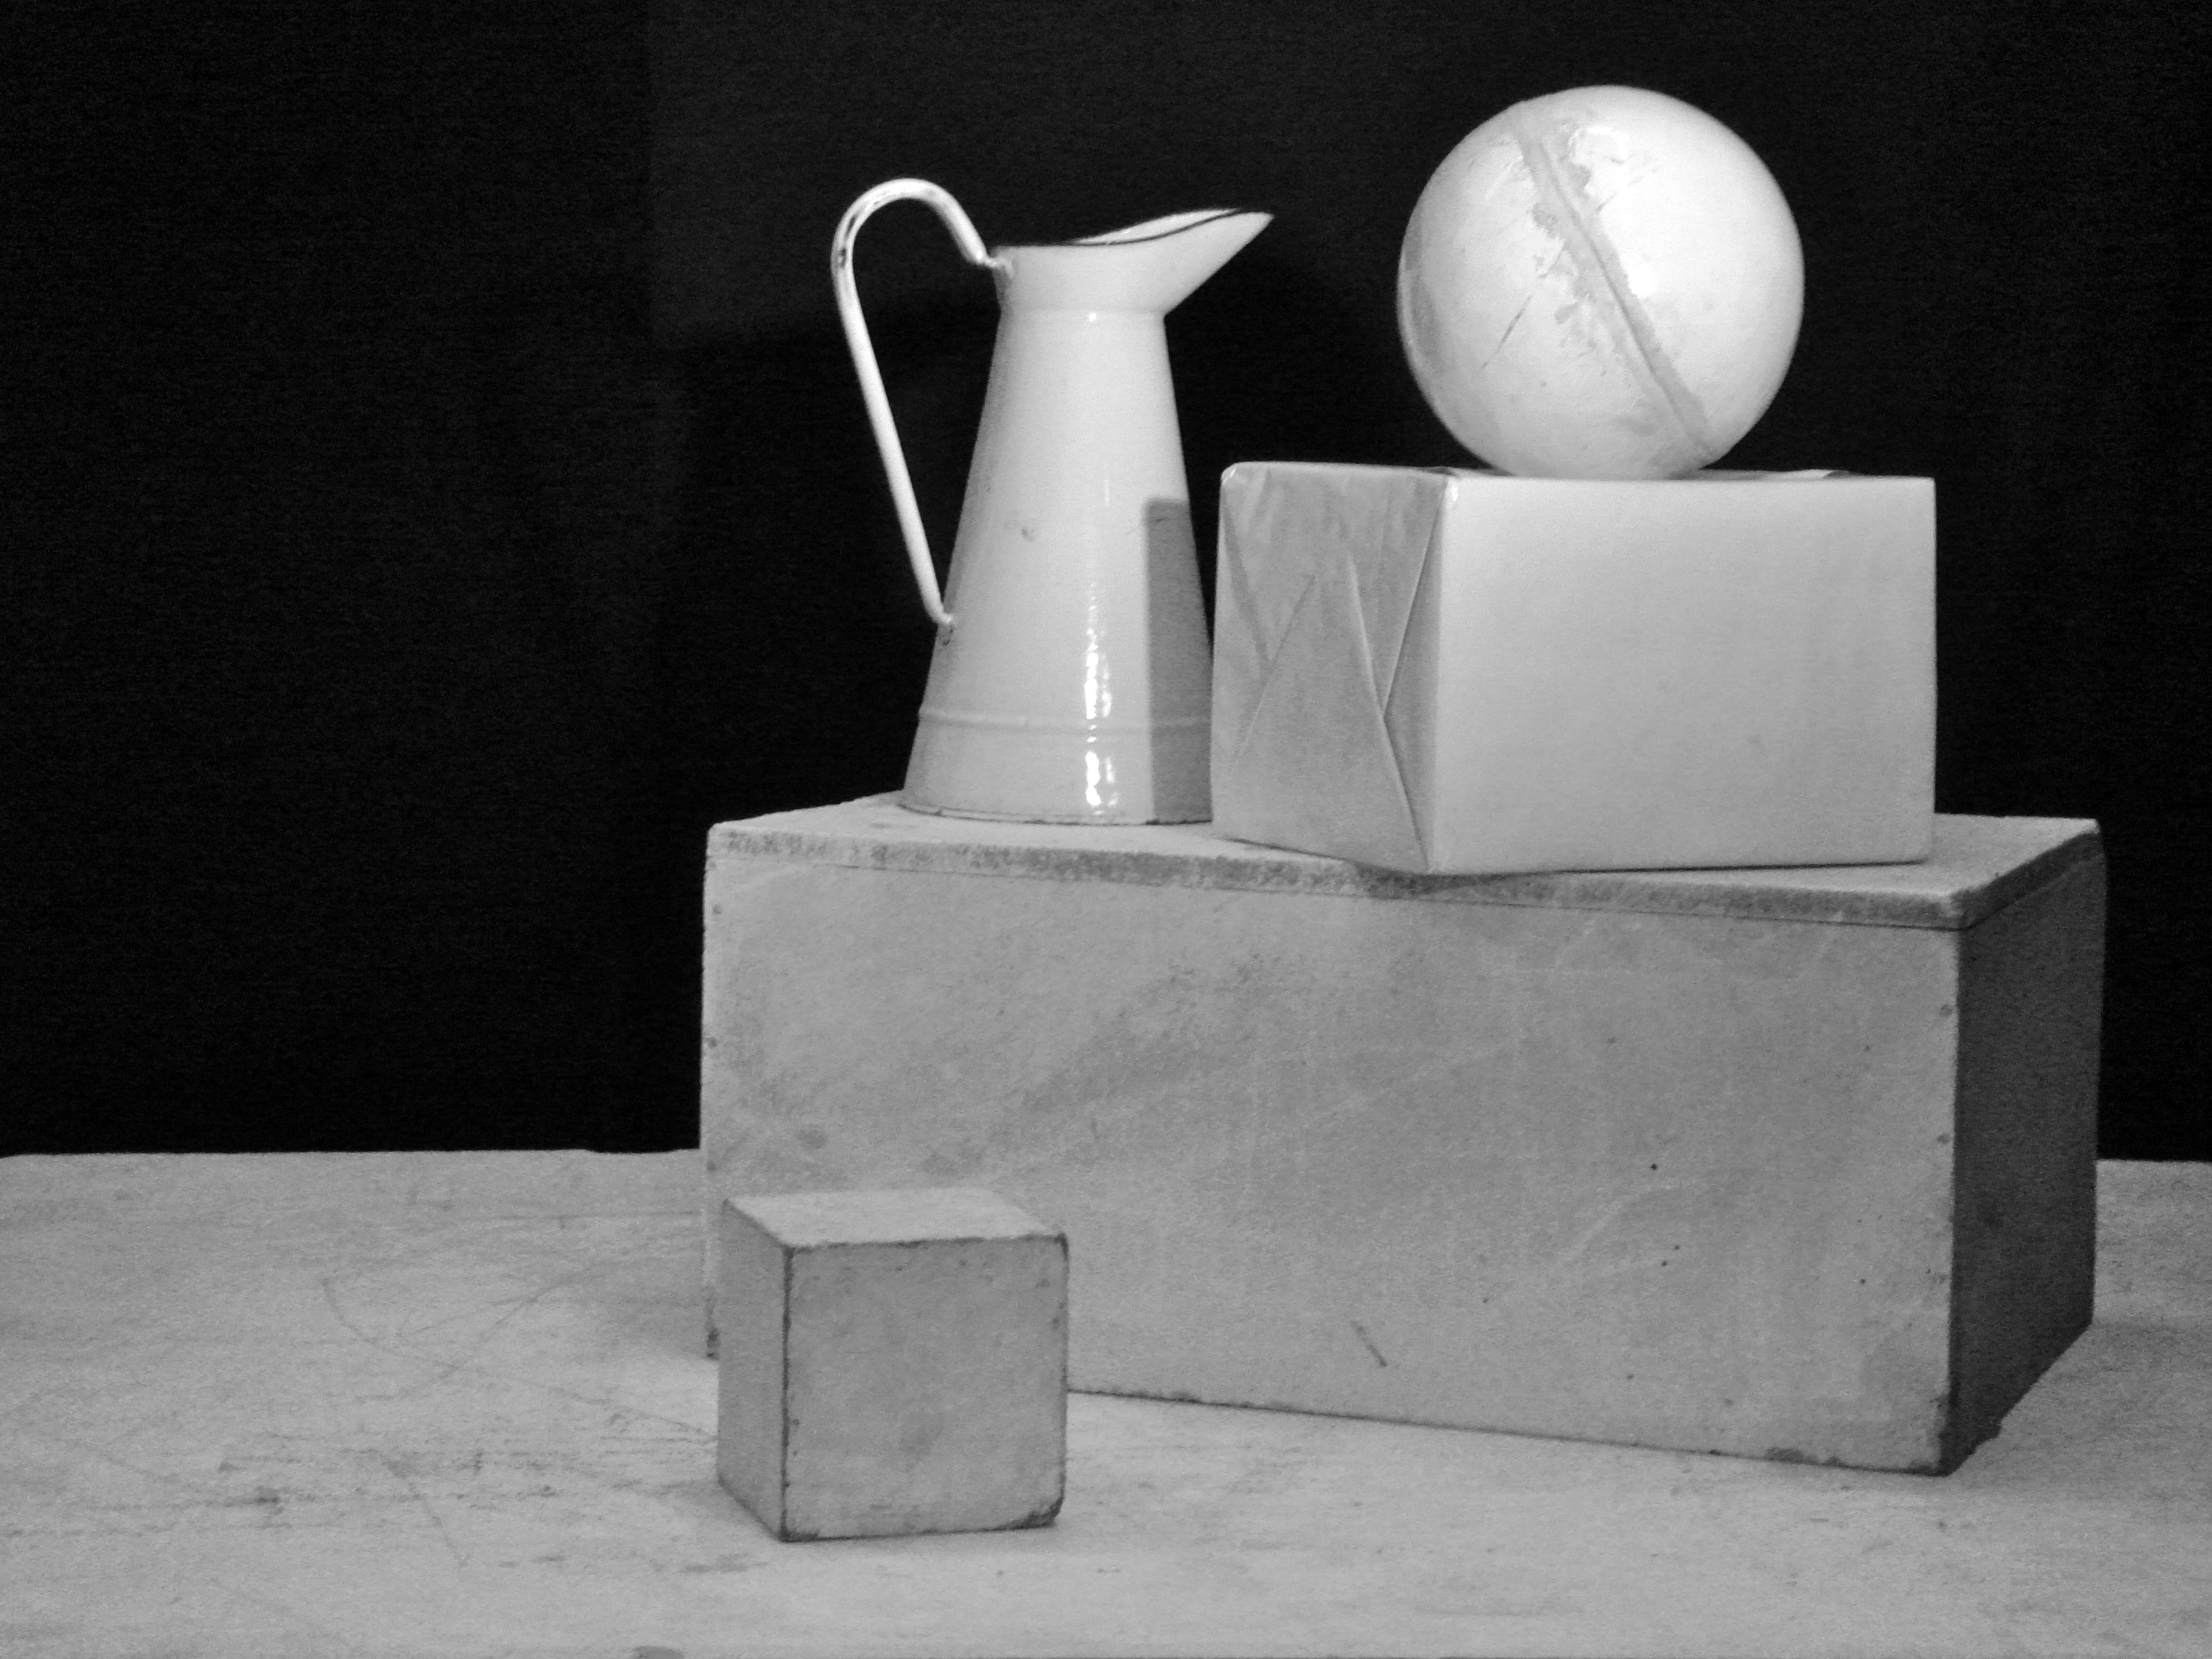
\includegraphics[width=0.95\textwidth]{geometria.jpg}
  \begin{center}
    {\large ``Geometria''}\par
    Foto di Ram\'on Peco\par
    \url{http://www.flickr.com/photos/desdetasmania/1606257376/}\par
    Licenza: Creative Commons Attribution 2.0\par
  \end{center}
\newpage


\section{La misura}

\subsection{Classi di grandezze omogenee}

L'obiettivo di questo paragrafo è quello di ottenere un procedimento teorico per misurare alcuni enti geometrici come segmenti, angoli, superfici, solidi. Non è possibile invece misurare punti, rette, semirette.
L'operazione del \emph{misurare} consiste sostanzialmente nell'assegnare a una grandezza geometrica, ma non solo, un numero ben definito. Questo numero si ottiene confrontando la grandezza da misurare con una grandezza di riferimento, detta \emph{misura campione}. Infatti, quello che ci interessa delle grandezze è il fatto di poterle confrontare tra di loro per stabilire qual è la più grande ed eventualmente effettuarne la somma.
In generale, gli oggetti che ci circondano hanno delle caratteristiche: lunghezza, peso, forma, altezza, superficie, colore, temperatura, morbidezza, \ldots{} Alcune di queste caratteristiche sono confrontabili tra loro, per esempio la lunghezza di due segmenti o il peso di due corpi; altre non sono confrontabili. Le caratteristiche che si possono confrontare si dicono omogenee. Ci sono poi caratteristiche che sono additive, cioè si possono addizionare. Queste caratteristiche che hanno la peculiarità di essere confrontabili e sommabili si chiamano grandezze.
Nei capitoli precedenti abbiamo visto come confrontare e sommare segmenti, confrontare e sommare angoli. Vogliamo fare la stessa cosa con gli archi di circonferenza, le superfici e i volumi.
Non possiamo evidentemente confrontare e sommare punti, perché i punti sono tutti congruenti tra loro e sommando due punti non otteniamo un altro punto ma rimangono gli stessi due punti. Non possiamo confrontare rette perché sono tutte congruenti tra loro e non possiamo sommarle perché non otterremmo un'altra retta. Non possiamo per esempio sommare due triangoli. Né possiamo confrontare segmenti con angoli perché non sono grandezze omogenee, cioè non sono dello stesso tipo; non possiamo confrontare angoli con superfici perché anche questo non sono grandezze tra loro omogenee, \ldots{}
Diamo ora il concetto generale di classe di grandezze.
\begin{definizione}
Un insieme di grandezze geometriche si dice che forma una \emph{classe di grandezze} quando:
\begin{itemize*}
\item date due qualunque grandezze, è sempre possibile confrontarle, cioè stabilire se sono uguali o, in caso contrario, quali di esse sia la maggiore e quale la minore;
\item è sempre possibile definire un'operazione di somma tra grandezze che goda delle proprietà associativa e commutativa.
\end{itemize*}
Le grandezze di una stessa classe si dicono tra loro \emph{omogenee}.
\end{definizione}

A partire da questa definizione possiamo dare quella di multiplo e sottomultiplo.
\begin{definizione}
Data una grandezza geometrica $A$ ed un numero naturale $n$, la grandezza geometrica $B$ si dice \emph{multipla} di $A$ secondo il numero $n$ se è data dalla somma di $n$ grandezze tutte uguali ad $A$ e scriveremo $B=n\cdot A$. In questo caso $A$ è definita grandezza \emph{sottomultipla} di $B$ secondo il numero naturale $n$ e scriviamo $A=\dfrac{B}{n}$.
\end{definizione}

Dato un segmento $AB$ possiamo dare un significato alla scrittura $\dfrac{3}{2}AB$ nel seguente modo:

%figura

Il segmento $AB$ è costituito da 3 segmenti ciascuno congruente alla metà di $AB$.
\begin{definizione}
Due grandezze omogenee $A$ e $B$ si dicono \emph{commensurabili} quando esiste una terza grandezza $C$, ad esse omogenea, che è sottomultipla sia di $A$ che di $B$: $A=n\cdot C$, $B=m\cdot C$.
Due grandezze omogenee $A$ e $B$ si dicono \emph{incommensurabili} quando non esiste una terza grandezza $C$, ad esse omogenea, che sia sottomultipla sia di $A$ che di $B$.
\end{definizione}

L'esistenza di grandezze incommensurabili è confermata dal seguente teorema.
\begin{teorema}
Il lato e la diagonale di un quadrato sono grandezze incommensurabili.
\end{teorema}

\begin{proof}
La dimostrazione si sviluppa per assurdo. Con riferimento alla figura, verifichiamo che  il lato $AB$ e la diagonale $AC$ del quadrato $ABCD$ sono incommensurabili.
Per assurdo, supponiamo che esista una grandezza $U$, omogenea sia al lato sia alla diagonale, che sia un sottomultiplo comune, cioè $AC=n\cdot U$ e $AB=m\cdot U$.
Per il teorema di Pitagora $AC^2=AB^2+BC^2$ e poiché $AB=BC$ si ha $AC^2=AB^2+AB^2=2\cdot AB^2$. Tenendo conto che $AC=n\cdot U$ e $AB=m\cdot U$ la formula precedente ci permette di affermare che $n^2\cdot U^2=2m^2\cdot U^2$. Dividendo per $U^2$ ambo i membri dell'uguaglianza otteniamo $n^2=2m^2$, dove $n$ e $m$ sono due numeri naturali. \`E abbastanza facile dimostrare che questa uguaglianza non può sussistere. Infatti, se $m$ è un numero pari allora $m^2$ avrà un numero pari di fattori uguali a 2 e quindi $2m^2$ avrà un numero dispari di fattori uguali a 2, ciò implica che anche $n^2$ deve avere un numero dispari di fattori uguali a 2; se $m$ è dispari allora $2m^2$ avrà un solo fattore uguale a 2 e di conseguenza non può essere uguale al quadrato di un numero $n$. Da cui l'assurdo che $m$ non può essere né pari né dispari.
\end{proof}

Storicamente, questa è stata la prima scoperta di grandezze incommensurabili, probabilmente dovuta al Ippaso di Metaponto, matematico vissuto tra Crotone e Metaponto (Calabria e Basilicata) nel 500 \aC circa. La tradizione dice che morì in un naufragio per aver rivelato la scoperta dell'esistenza delle grandezze incommensurabili, in contrasto con il pensiero del maestro Pitagora.
Siano $A$ e $B$ due grandezze omogenee commensurabili, sia $C$ la grandezza sottomultipla in comune, si avrà $A=n\cdot C$ e $B=m\cdot C$. Da cui $C=\dfrac{1}{n}A$ e $C=\dfrac{1}{m}B$. Dal confronto si ha $\dfrac{1}{n}A=\dfrac{1}{m}B$ da cui $A=\dfrac{n}{m}B$.

\begin{definizione}
Si dice \emph{rapporto di due grandezze omogenee} $A$ e $B$ il numero razionale $\dfrac{n}{m}$ tale che $A=\dfrac{n}{m}B$.
\end{definizione}
Occorre supporre la validità dei seguenti postulati.

\noindent \emph{Postulato della divisibilità.} Ogni grandezza geometrica è sempre divisibile in un numero qualunque di parti.

\noindent \emph{Postulato di Eudosso-Archimede.} Date due grandezze omogenee disuguali esiste sempre una grandezza multipla della minore che supera la maggiore.

Possiamo dare ora la definizione di misura di un segmento rispetto a un altro, nel caso in cui i due segmenti sono commensurabili.
\begin{definizione}
Date due grandezze $A$ e $U$ tra loro commensurabili si definisce \emph{misura di $A$ rispetto a $U$} il numero razionale $\dfrac{m}{n}$ per il quale $A=\dfrac{m}{n}U$. La grandezza $U$ viene detta \emph{unità di misura}.
\end{definizione}

Per le definizioni precedenti, la misura di $U$ rispetto a se stessa è evidentemente 1.

Solitamente si usa come unità di misura delle lunghezze il metro, con il suo multipli (decametro, ettometro, chilometro, \ldots{}) ed i suoi sottomultipli (decimetro, centimetro, millimetro, \ldots{}). Per misurare gli angoli si usa il grado che è la 360\textsuperscript{a} parte dell'angolo giro. Per misurare le superfici si usa come unità di superficie quella di un quadrato di lato 1 m (metro quadrato). Per misurare i solidi si usa il volume di un cubo di lato 1 m (metro cubo).

Circa la scrittura delle misure, in Italia valgono le seguenti norme: l'unità di misura si scrive sempre dopo il numero che la indica, tranne le misure monetarie: si scrive 12 m e non m 12; si scrive \officialeuro 12 e non 12 \officialeuro. L'unità di misura non è mai seguita dal puntino e non va mai espressa al plurale.

\`E possibile estendere la definizione di rapporto e la conseguente definizione di misura anche per la grandezze tra loro incommensurabili, come per esempio lato e diagonale dello stesso quadrato. Il percorso però è più lungo e complesso, poiché il rapporto tra due grandezze commensurabili è sempre un numero razionale mentre il rapporto tra due grandezze incommensurabili non è un numero razionale.

Partiamo dalla definizione di classi contigue.
\begin{definizione}
Due classi di grandezze omogenee si dicono \emph{contigue} se godono delle seguenti proprietà:
\begin{itemize*}
\item sono \emph{separate}: ogni grandezza della prima classe è minore di ogni grandezza della seconda classe. Vale a questo proposito il \emph{postulato della continuità}, secondo il quale due classi di grandezze separate ammettono almeno un elemento separatore (ne esiste sicuramente uno, ma potrebbero anche essercene infiniti), cioè una grandezza che sia maggiore (o uguale) di ogni grandezza della prima classe e minore (o uguale) di ogni grandezza della seconda.
\item godono della \emph{proprietà dell'avvicinamento indefinito}: presa una grandezza $\epsilon$, piccola a piacere, omogenea a quelle date, esiste sempre una grandezza della seconda classe ed una della prima la cui differenza sia minore di $\epsilon$.
\end{itemize*}
\end{definizione}

Per due classi di grandezze contigue vale l'\emph{assioma di Cantor}: due classi di grandezze contigue ammettono uno e un solo elemento separatore.

Basandoci sul concetto di contiguità possiamo a questo punto definire un qualunque \emph{numero irrazionale} come l'unico elemento separatore tra due classi contigue di numeri razionali; nella prima classe mettiamo tutti i numeri che approssimano il numero irrazionale per difetto e nella seconda quelli che lo approssimano per eccesso.

Prendendo come esempio il numero irrazionale $\sqrt{2}$ le due classi sono:
\[A: 1\quad \np{1,4}\quad \np{1,41}\quad \np{1,414}\quad \np{1,4142}\quad \ldots{}\]
\[B: 2\quad \np{1,5}\quad \np{1,42}\quad \np{1,415}\quad \np{1,4143}\quad \ldots{}\]
Si può osservare che le due successioni sono separate, in quanto ogni numero della prima è minore di ogni numero della seconda, inoltre godono della proprietà dell'avvicinamento indefinito, in quanto è sempre possibile trovare un numero razionale appartenente ad $A$ ed uno appartenente a $B$ la cui differenza sia minore di un qualsiasi numero $\epsilon$, per quanto piccolo questo si prenda.
Quindi, per l'assioma di Cantor, esiste ed è unico l'unico elemento separatore di queste due successioni; possiamo identificare questo numero con la coppia di successioni e scrivere: $\sqrt{2} = (A\text{, }B)$.

Questa definizione vale non solo per i numeri irrazionali, ma anche per quelli razionali. Per esempio, la frazione $\dfrac{15}{4}=3,75$ è definita dalle classi contigue:
\[A: 3\quad \np{3,7}\quad \np{3,74}\quad \np{3,749}\quad \np{3,7499}\quad \ldots{}\]
\[B: 4\quad \np{3,8}\quad \np{3,75}\quad \np{3,750}\quad \np{3,7501}\quad \ldots{}\]

Possiamo naturalmente definire in questo modo anche i numeri interi. Per esempio 5 è l'elemento separatore delle classi:
\[A: 4\quad \np{4,9}\quad \np{4,99}\quad \np{4,999}\quad \np{4,9999}\quad \ldots{}\]
\[B: 6\quad \np{5,1}\quad \np{5,01}\quad \np{5,001}\quad \np{5,0001}\quad \ldots{}\]

Concludiamo quindi affermando che un qualunque numero reale $r$ può essere definito come l'elemento separatore di una coppia di classi numeriche contigue.

I numeri reali sono pertanto il raggruppamento di numero razionali e irrazionali:

% figura -- \usetikzlibrary{decorations.pathreplacing}

Passiamo ora a definire la misura delle grandezze incommensurabili.

Date le lunghezze incommensurabili AB e CD, poniamo
\[A=\left\{\dfrac{m}{n}\in\insQ^+\mid\dfrac{m}{n}CD<AB\right\}\qquad\text{e}\qquad B=\left\{\dfrac{m}{n}\in\insQ^+\mid\dfrac{m}{n}CD>AB\right\}.\]
Si dimostra che la coppia $(A\text{, }B)$ è una coppia di classi contigue di $\insQ^+$. In maniera intuitiva possiamo dire che $A$ contiene i valori approssimati per difetto e $B$ contiene i valori approssimati per eccesso del rapporto $\dfrac{m}{n}$.
Chiamiamo \emph{rapporto fra le lunghe incommensurabili} $AB$ e $CD$ il numero irrazionale dato dalle classi contigue $(A\text{, }B)$.


\section{Proporzionalità tra grandezze}

\begin{definizione}
Date quattro grandezze $A$, $B$, $C$ e $D$, le prime due omogenee tra loro così come le ultime due, queste formano una \emph{proporzione} se il rapporto delle prime due è uguale al rapporto delle ultime due. Si scrive
\[ A : B = C : D\]
e si legge ``$A$ sta a $B$ come $C$ sta a $D$''.
\end{definizione}

\begin{definizione}
In una proporzione
\begin{itemize*}
\item il primo ed il terzo termine ($A$ e $C$) si chiamano \emph{antecedenti};
\item il secondo ed il quarto termine ($B$ e $D$) si chiamano \emph{conseguenti};
\item $B$ e $C$ si chiamano \emph{medi};
\item $A$ e $D$ si chiamano \emph{estremi};
\item la grandezza $D$ si chiama \emph{quarta proporzionale}.
\end{itemize*}
\end{definizione}

\begin{definizione}
Se in una proporzione tra grandezze tutte omogenee i medi sono uguali tra loro $A : B = B : C$, la proporzione si dice \emph{continua}, la grandezza $B$ si chiama \emph{media proporzionale} e la grandezza $C$ si dice \emph{terza proporzionale}.
\end{definizione}

\begin{teorema}[fondamentale delle proporsioni]
Condizione necessaria e sufficiente affinché quattro grandezze siano in proporzione è che siano in proporzione le loro misure.
\end{teorema}

\begin{proof}
Siano $A$ e $B$ due grandezze omogenee, $a$ e $b$ le loro misure rispetto ad un'unità di misura omogenea ad $A$ e $B$; $C$ e $D$ due grandezze anch'esse omogenee tra loro e $c$ e $d$ le loro misure rispetto ad un'unità di misura omogenea a $C$ e $D$.
\begin{enumerate*}
\item (condizione necessaria $\Rightarrow$)\\
Dimostriamo innanzitutto che la condizione è necessaria: supposto che le quattro grandezze siano in proporzione, dimostriamo che sono in proporzione le loro misure.\\
Ipotesi: $A : B = C : D$ \tab Tesi: $a : b = c : d$.\\
Applicando il teorema secondo cui il rapporto tra due grandezze è uguale al quoziente delle loro misure, avremo $\dfrac{A}{B}=\dfrac{a}{b}$ e $\dfrac{C}{D}=\dfrac{c}{d}$. Ma per ipotesi $\dfrac{A}{B}=\dfrac{C}{D}$ e quindi, per la proprietà transitiva dell'uguaglianza, avremo che $\dfrac{a}{b}=\dfrac{c}{d}$, che si può anche scrivere nella forma $a : b = c : d$.

\item (condizione sufficiente $\Leftarrow$)\\
Dimostriamo ora che la condizione è sufficiente.\\
Ipotesi: $a : b = c : d$\tab Tesi: $A : B = C : D$.\\
Sempre dal teorema citato precedentemente, poiché $\dfrac{A}{B}=\dfrac{a}{b}$ e $\dfrac{C}{D}=\dfrac{c}{d}$, per la proprietà transitiva dell'uguaglianza avremo che $\dfrac{a}{b}=\dfrac{C}{D}$, vale a dire $A : B = C : D$.
\end{enumerate*}
\end{proof}

Ricordiamo che per la proporzionalità tra numeri vale la seguente
\begin{proprieta}
Condizione necessaria e sufficiente affinché quattro numeri siano in proporzione è che il prodotto dei medi sia uguale al prodotto degli estremi.
\end{proprieta}

\subsection{Proprietà delle proporzioni}

Grazie al teorema fondamentale delle proporzioni possiamo trasferire le proprietà delle proporzioni tra numeri alle proporzioni tra grandezze.

\begin{enumerate*}
\item \textbf{Proprietà dell'invertire}\\
Scambiando ogni antecedente col proprio conseguente otteniamo una nuova proporzione equivalente alla precedente.
\[A : B = C : D \:\Rightarrow\: B : A = D : C.\]

\item \textbf{Proprietà del permutare}
Se le quattro grandezze sono tutte omogenee, possiamo scambiare tra loro i medi o gli estremi, ed otterremo sempre una nuova proporzione equivalente alla precedente.
\[A : B = C : D \:\Rightarrow\: D : B = C : A.\]

\item \textbf{Proprietà del comporre}
La somma delle prime due grandezze sta alla prima (o alla seconda) grandezza come la somma delle altre due sta alla terza (o alla quarta).
\[A : B = C : D \:\Rightarrow\: (A + B) : A = (C + D) : C\qquad\text{e}\qquad A : B = C : D \:\Rightarrow\: (A + B) : B = (C + D) : D\]

\item \textbf{Proprietà dello scomporre}
La differenza tra la prima e la seconda grandezza sta alla prima (o alla seconda) grandezza come la differenza tra le altre due sta alla terza (o alla quarta). Questa proprietà richiede che ogni antecedente sia  maggiore del proprio conseguente. Se dunque $A > B$ e $C > D$ avremo che
\[A : B = C : D \:\Rightarrow\: (A - B) : A = (C - D) : C\qquad\text{e}\qquad A : B = C : D \:\Rightarrow\: (A - B) : B = (C - D) : D\]
\end{enumerate*}

In riferimento alla disuguaglianza precedente, va precisato che se quattro grandezze sono in proporzione, tra antecedenti e conseguenti intercorre sempre la stessa relazione, vale a dire che se la prima grandezza è uguale, maggiore o minore della seconda, anche la terza sarà uguale, maggiore o minore della quarta.

\begin{teorema}[della quarta proporzionale]
Date tre grandezze $A$, $B$ e $C$, con $A$ e $B$ omogenee tra loro, esiste ed è unica una grandezza $D$, omogenea alla terza, che con le tre date formi una proporzione.
\end{teorema}

\begin{proof}
Siano $A$, $B$ e $C$ tre grandezze, le prime due omogenee tra loro. Supponiamo che esista una quarta grandezza $X$, omogenea a $C$, tale che valga la proporzione $A : B = C : X$.
Sostituendo alle grandezze le loro misure, per il teorema fondamentale dovrà essere $a : b = c : x$.
Applichiamo ora la proprietà fondamentale delle proporzioni numeriche, uguagliando il prodotto dei medi a quello degli estremi $ax = bc$.
Risolvendo l'equazione in $x$ otteniamo $x = \dfrac{bc}{a}$, e poiché $a$, $b$ e $c$ sono diversi da zero (e positivi), in quanto misure di grandezze geometriche, quest'equazione avrà come soluzione uno e un solo numero reale (positivo), in quanto la soluzione di un'equazione di primo grado, se esiste, è unica.
Questo numero reale sarà quindi la misura della quarta grandezza $X$, e poiché tra grandezze omogenee ad ogni numero reale corrisponde una e una sola grandezza, questa quarta proporzionale esiste ed è unica.
\end{proof}

\subsection{Grandezze direttamente e inversamente proprozionali}

Consideriamo due classi di grandezze
\[A\text{,}\quad B\text{,}\quad C\text{,}\quad D\text{,}\quad \ldots{}\]
\[A'\text{,}\quad B'\text{,}\quad C'\text{,}\quad D'\text{,}\quad \ldots{}\]
Queste due classi si dicono in \emph{corrispondenza biunivoca} quando ad ogni grandezza della prima classe corrisponde una e una sola grandezza della seconda e viceversa.
Le grandezze $A$ e $A'$, $B$ e $B'$, $C$ e $C'$, $D$ e $D'$, \ldots{} si dicono \emph{corrispondenti}.

Le grandezze di queste due classi si dicono \emph{direttamente proporzionali} quando il rapporto di due grandezze qualunque della prima classe è uguale al rapporto delle due grandezze corrispondenti della seconda classe, cioè quando valgono le proporzioni
\[A : B = A' : B'\qquad\qquad A : C = A' : C'\qquad\qquad B : C = B' : C'\qquad\qquad\ldots{}\]
Se poi le grandezze della prima classe sono omogenee con quelle della seconda, allora possiamo permutare i medi
\[A : A' = B : B'\qquad\qquad A : A' = C : C'\qquad\qquad B : B' = C : C'\qquad\qquad\ldots{}\]
E, applicando la proprietà transitiva dell'uguaglianza, otteniamo
\[A : A' = B : B' = C : C' = \ldots{} = k\]
da cui segue che il rapporto tra due grandezze corrispondenti è costante. Questo rapporto costante è un numero detto \emph{costante di proporzionalità}.

Se le grandezze della prima classe non fossero omogenee con quelle della seconda, dovremmo passare dalla proporzionalità tra le grandezze a quella tra le loro misure (reso sempre possibile dal teorema fondamentale), ed in questo caso sarebbe il rapporto tra le loro misure ad essere costante.

Per determinare se due classi di grandezze sono direttamente proporzionali si applica il seguente teorema
\begin{teorema}\label{teo:6.1}
Condizione necessaria e sufficiente affinché due classi di grandezze in corrispondenza biunivoca siano direttamente proporzionali è che
\begin{itemize*}
\item a grandezze uguali della prima classe corrispondano grandezze uguali della seconda;
\item alla somma di due o più grandezze della prima classe corrisponda la somma delle grandezze corrispondenti della seconda classe.
\end{itemize*}
\end{teorema}

\begin{proof}~\\
\begin{itemize*}
\item (condizione necessaria $\Rightarrow$)\\
Dimostriamo che la condizione è necessaria, cioè che se le grandezze sono proporzionali, allora devono valere le due proprietà.
Dette $A$ e $B$ due grandezze della prima classe, e $A'$, $B'$ le grandezze corrispondenti della seconda classe, per ipotesi avremo $A : B = A' : B'$.
Se $A=B$, il loro rapporto è 1, e tale deve essere il rapporto tra $A'$ e $B'$, da cui segue $A' = B'$.
Quindi la prima proprietà è verificata.
Applichiamo ora alla proporzione data la proprietà del comporre $(A + B) : A = (A' + B') : A'$.
Se $C$ è la grandezza della prima classe tale che $C = A + B$, sostituendo nella proporzione avremo:
$C : A = (A' + B') : A'$.
Se $C'$ è la grandezza che corrisponde a $C$, poiché per ipotesi le due classi di grandezze sono direttamente proporzionali, dovrà valere anche la seguente proporzione $(A + B) : A = C' : A'$, e per l'unicità della quarta proporzionale dovrà essere $C' = A' + B'$.
Anche la seconda proprietà risulta dunque verificata.
\item (condizione sufficiente $\Leftarrow$)\\
Dimostriamo ora che la condizione è sufficiente:  se valgono le due proprietà, le due classi di grandezze sono direttamente proporzionali.
Consideriamo due grandezze qualunque della prima classe $A$ e $B$; possono essere uguali o disuguali.
Se $A = B$, allora per la prima proprietà sarà pure $A' = B'$; poiché $A : B = 1$ e $A' : B' = 1$, per la proprietà transitiva dell'uguaglianza dovrà essere $A : B = A' : B'$, quindi il rapporto tra due grandezze qualunque della prima classe è uguale al rapporto delle grandezze corrispondenti della seconda, e perciò le due classi di grandezze sono direttamente proporzionali.
Supponiamo ora $A$ e $B$ disuguali, sia ad esempio $A > B$. Questo vuol dire che esiste una terza grandezza $C$ tale che $A = B + C$. Per la seconda proprietà a $B + C$ corrisponde $B' + C'$ e per la prima proprietà ad $A = B + C$ corrisponde $A' = B' + C'$, da cui si deduce che $A' > B'$.
Analogamente si dimostra che se $A < B$, allora $A' < B'$.

Sempre per la seconda proprietà, moltiplicando le grandezze per uno stesso numero naturale avremo che ad $n\cdot A$ corrisponderà $n\cdot A'$ e ad $m\cdot B$ corrisponderà $m\cdot B'$. Per quanto premesso, avremo che se $n\cdot A = m\cdot B$, sarà anche $n\cdot A' = m\cdot B'$; se $n\cdot A > m\cdot B$, sarà anche $n\cdot A' > m\cdot B'$ ed infine, se $n\cdot A < m\cdot B$, ne deriverà che $n\cdot A' < m\cdot B'$.
Questo vuol dire che, andando a costruire il rapporto tra le grandezze, avremo
\[\dfrac{A}{B} = \dfrac{m}{n} \:\Leftarrow\: \dfrac{A'}{B'} = \dfrac{m}{n}\qquad \dfrac{A}{B} > \dfrac{m}{n} \:\Leftarrow\: \dfrac{A'}{B'} > \dfrac{m}{n}\qquad \dfrac{A}{B} < \dfrac{m}{n} \:\Leftarrow\: \dfrac{A'}{B'} < \dfrac{m}{n}.\]
 
Dunque i rapporti $\dfrac{A}{B}$ e $\dfrac{A'}{B'}$ ammettono gli stessi valori approssimati per difetto o per eccesso, e quindi questi rapporti rappresentano lo stesso numero reale. Per cui, concludendo, si ha $A : B = A' : B'$.
\end{itemize*}
\end{proof}

\subsection{Grandezze inversamente proporzionali}

Le grandezze di due classi in corrispondenza biunivoca si dicono inversamente proporzionali quando il rapporto di due grandezze qualunque della prima classe è uguale al rapporto inverso delle due grandezze corrispondenti della seconda classe, cioè quando valgono le proporzioni
\[A : B = B' : A'\qquad\qquad A : C = C' : A'\qquad\qquad B : C = C' : B'\qquad\qquad \ldots{}\]
Se dalla proporzionalità tra le grandezze passiamo a quella tra le loro misure avremo
\[a : b = b' : a'\qquad\qquad a : c = c' : a'\qquad\qquad b : c = c' : b'\qquad\qquad \ldots{}\]
Applicando la proprietà fondamentale della proporzionalità tra numeri (il prodotto dei medi è uguale al prodotto degli estremi) avremo
\[aa' = bb'\qquad\qquad aa' = cc'\qquad\qquad bb' = cc'\qquad\qquad \ldots{}\]
E, applicando la proprietà transitiva dell'uguaglianza
\[aa' = bb' = cc' = \ldots{} =k\]
da cui segue che il prodotto tra le misure di due grandezze corrispondenti è costante. Anche in questo caso il prodotto costante è un numero detto costante di proporzionalità.

Teoremi su particolari classi di grandezze direttamente proporzionali
\begin{teorema}\label{teo:6.2}
I rettangoli aventi altezze congruenti sono proporzionali alle rispettive basi.
\end{teorema}

\begin{proof}
Consideriamo la classe di grandezze costituita da tutti i rettangoli con altezze congruenti e la classe costituita dalle rispettive basi. Queste due classi sono in corrispondenza biunivoca, in quanto ad ogni rettangolo corrisponde una ed una sola base e viceversa.
Per dimostrare che queste due classi sono direttamente proporzionali applichiamo il teorema~\ref{teo:6.1} dimostrato precedentemente. Dobbiamo cioè verificare che siano soddisfatte le due proprietà.

\emph{Prima proprietà: a grandezze uguali della prima classe devono corrispondere grandezze uguali della seconda.}\\
Si nota facilmente che questa proprietà è sempre verificata, in quanto se si suppone che $AB = CD$, allora anche i rettangoli che hanno questi segmenti come base, avendo le altezze congruenti, saranno sicuramente congruenti.

\emph{Seconda proprietà: ad un segmento che sia la somma di due segmenti deve corrispondere un rettangolo che sia la somma di due rettangoli aventi quei segmenti come base.}\\
Supponiamo infatti $EG =  AB + CD$; prendiamo su $EG$ il punto $F$ che divida il segmento in due parti: $EF=AB$, $FG=CD$. Tracciando la perpendicolare in $F$ ad $EG$, questa divide il rettangolo $R_3$ in due rettangoli rispettivamente congruenti ad $R_1$ e ad $R_2$, e quindi $R_3= R_1+R_2$.

Poiché dunque valgono le due proprietà richieste dal teorema, avremo che $R_1 : R_2 = AB : CD$, 
$R_2 : R_3 = CD  : EG$, \ldots{} e quindi le due classi di grandezze sono direttamente proporzionali.
\end{proof}

In modo analogo si dimostra che:
\begin{itemize*}
\item I rettangoli aventi basi congruenti sono direttamente proporzionali alle rispettive altezze.
\item Gli archi di un stessa circonferenza sono direttamente proporzionali ai corrispondenti angoli al centro.
\end{itemize*}


\section{Teorema di Talete, caso generale}

\begin{teorema}[di Talete]
Un fascio di rette parallele determina su due trasversali classi di segmenti direttamente proporzionali.
\end{teorema}

\begin{proof}
Assumiamo come ipotesi di avere cinque rette parallele $a$, $b$, $c$, $d$ ed $e$. Dimostriamo che sono proporzione i segmenti 
$AB : A'B' = BC : B'C' = AC : A'C' = BD : B'D' = \ldots{}$

A questo scopo ricorriamo alla condizione necessaria e sufficiente sulla proporzionalità tra grandezze (teorema~\ref{teo:6.1}):
condizione necessaria e sufficiente affinché due classi di grandezze in corrispondenza biunivoca siano direttamente proporzionali è che
\begin{itemize*}
\item a grandezze uguali della prima classe corrispondano grandezze uguali della seconda;
\item alla somma di due o più grandezze della prima classe corrisponda la somma delle grandezze corrispondenti della seconda classe.
\end{itemize*}

La prima proprietà è stata dimostrata nel capitolo~\ref{chap:circonferenza}, dove è stato esposto il teorema di Talete: a segmenti congruenti su una trasversale corrispondono segmenti congruenti sull'altra trasversale.

Dimostriamo allora che vale anche la seconda proprietà.
Consideriamo il fascio di rette parallele tagliato da due trasversali della figura.
Abbiamo come ipotesi che $CD = AB + BC$ e dobbiamo dimostrare che $C'D' = A'B' + B'C'$.

Poiché $CD = AB + BC$, determiniamo al suo interno il punto $E$ che lo divide nei due segmenti $CE=AB$ e $ED=BC$. Tracciamo la parallela alle rette date passante per $F$, che intersecherà la trasversale $t'$ nel punto $F'$. Per la prima parte del teorema, avremo che da $CF=AB$ segue che $C'F' = A'B'$ e da $FD = BC$ segue che $F'D'=B'C'$. Ma $C'D'=C'F' + F'D' = A'B' + B'C'$.
\end{proof}

\subsection{Conseguenze del teorema di Talete}

Dal teorema di Talete discendono due importanti corollari.
\begin{corollario}\label{cor:6.1}
Una retta parallela ad un lato di un triangolo determina sugli altri due lati, o sui loro prolungamenti, segmenti proporzionali.
\end{corollario}

\begin{proof}
Sia $ABC$ il triangolo in questione. Tracciamo una retta parallela al lato $BC$ che intersechi gli altri due nei punti $D$ ed $E$. Vogliamo dimostrare che $AE : AD = EC : DB$.

Tracciamo una retta passante per $A$ e parallela a $DE$ ed a $BC$. Ci troviamo così nelle condizioni di poter applicare il teorema di Talete, in quanto abbiamo tre rette parallele tagliate da due trasversali ($AB$ ed $AC$), per cui possiamo scrivere la proporzione tra segmenti corrispondenti $AE : AD = EC : DB$.
La stessa dimostrazione vale nel caso in cui la parallela al lato $BC$ interseca i prolungamenti dei lati $AB$ e $AC$.
\end{proof}

\begin{corollario}\label{cor:6.2}
La retta che divide due lati di un triangolo (o i loro prolungamenti) in segmenti proporzionali è parallela al terzo lato.
\end{corollario}

\begin{proof}
Abbiamo in ipotesi che $AE : AD = AC : AB$ e dobbiamo dimostrare che $DE$ è parallela a $BC$.

Ragioniamo per assurdo; neghiamo quindi la tesi e supponiamo che DE non sia parallela a $BC$. Esisterà allora un'altra retta passante per $D$ parallela a $BC$; questa retta intersecherà il lato $AC$ in un punto $F$. Per il corollario~\ref{cor:6.1} avremo che $AF : AD = AC : AB$.
Ma per il teorema della quarta proporzionale sappiamo che la quarta grandezza che con le tre date forma una proporzione deve essere unica, e quindi il punto $F$ deve coincidere con $E$ e la retta $DF$ coincidere con la retta $DE$, che perciò è parallela a $BC$.
\end{proof}

Un'altra importante conseguenza del teorema di Talete è il \emph{teorema della bisettrice}.
\begin{teorema}[della bisettrice]
La bisettrice di un angolo interno di un triangolo divide il lato opposto in parti proporzionali agli altri due lati.
\end{teorema}

\noindent Ipotesi: $A\widehat{B}D\cong D\widehat{B}C$.\tab Tesi: $AD : DC = AB : BC$.

\begin{proof}
Dal vertice $C$ tracciamo la parallela alla bisettrice $BD$ che incontra il prolungamento del lato $AB$ in $E$. Notiamo le seguenti congruenze tra angoli: $A\widehat{D}B\cong B\widehat{E}C$ in quanto corrispondenti rispetto alle parallele $BD$ ed $EC$ tagliate da $AE$; $D\widehat{B}C\cong B\widehat{C}E$ in quanto alterni interni rispetto alle parallele $BD$ ed $EC$ tagliate da $BC$.
Confrontando queste congruenze con quella in ipotesi ed applicando la proprietà transitiva della congruenza possiamo scrivere $B\widehat{E}C\cong B\widehat{C}E$. Dunque il triangolo $BEC$ è isoscele e per questo ha due lati congruenti $BE = BC$.
Applichiamo ora il primo corollario del teorema di Talete (corollario~\ref{cor:6.1}) al triangolo $AEC$. Si ha $AB : BE = AD : DC$. 
Per quanto appena dimostrato possiamo sostituire $BC$ a $BE$ ed avremo $AB : BC = AD : DC$.
\end{proof}

\subsubsection{Dividere un dato segmento in parti direttamente proporzionali a più segmenti dati}

Sia $PQ$ il segmento da dividere in parti direttamente proporzionali a tre segmenti dati $a$, $b$ e $c$.
Da un suo estremo, ad esempio $P$, si tracci una semiretta (non contenente $Q$) e su di essa si prendano i segmenti $PA$, $AB$ e $BC$ rispettivamente congruenti ad $a$, $b$ e $c$; si unisca $C$ con $Q$ e si traccino per $A$ e per $B$ le parallele a $CQ$ che incontrano il segmento $PQ$ rispettivamente in $A'$ e $B'$. Il segmento $PQ$ risulta così diviso nei segmenti $PA'$, $A'B'$ e $B'Q$ che, per il teorema di Talete, sono direttamente proporzionali ai segmenti $a$, $b$ e $c$.

Da notare che se i segmenti dati fossero tutti fra loro congruenti, il problema equivarrebbe a quello della divisione di un dato segmento in un numero assegnato di parti congruenti.

\subsubsection{Costruire il segmento quarto proporzionale dopo tre segmenti dati}

Siano $a$, $b$, $c$ i tre segmenti dati; si vuol costruire un segmento $d$ tale che valga la proporzione $a:b=c:d$.
Si consideri un angolo di vertice $O$ e su un suo lato si prendano i punti $A$ e $B$ tali che i segmenti $OA$ ed $AB$ siano congruenti rispettivamente ai segmenti $a$ e $b$; sull'altro lato dell'angolo si prenda il punto $C$ tale che il segmento $OC$ sia congruente al segmento $c$. Si traccino la retta $AC$ e la parallela ad essa per $B$, indicando con $D$ il punto in cui quest'ultima incontra la semiretta $OC$. Per il teorema di Talete il segmento $CD$ è il quarto proporzionale richiesto. 

Si noti che, per il teorema della quarta proporzionale, il segmento richiesto è unico, quindi si giunge allo stesso segmento indipendentemente dall'angolo utilizzato nella costruzione. 

Nel caso particolare in cui $b = c$, la costruzione appena descritta consente di trovare il segmento terzo proporzionale a due segmenti dati.

\subsubsection{Proprietà}

Dato un angolo di vertice $V$ e lati due semirette $r$ ed $s$, staccare su $r$ il segmento $VR_5$ e su $S$ il segmento $VS_1$, di lunghezza arbitraria. Successivamente, usando un compasso, staccare su $s$ i segmenti $S_1S_2$, $S_2S_3$, $S_3S_4$ e $S_4S_5$, tutti congruenti a $VS_1$. Dimostrare che, tracciando la retta per $R_5S_5$ e le corrispondenti parallele per $S_1$, $S_2$, $S_3$ ed $S_4$, il segmento $VR_5$ risulta suddiviso in parti uguali.

Osservando che questo procedimento può essere esteso per induzione a qualunque numero finito di segmenti, si può constatare che la divisibilità di un segmento in parti uguali non è un postulato autonomo, ma una proprietà intrinseca della geometria euclidea.


\section{Avere la stessa forma}

Osserviamo le coppie di figure sotto rappresentate e cerchiamo di capire cosa intendiamo dire quando affermiamo che due figure hanno  la stessa forma.

I due cerchi della figura hanno certamente la stessa forma.

In questa figura i poligoni $P_1$ e $P_2$ hanno gli angoli rispettivamente congruenti, ma non possiamo dire che abbiano la stessa forma.

In questa figura osserviamo che i lati di $HKLM$ sono rispettivamente la metà dei lati di $DEFG$, ma anche in questo caso non possiamo dire che i due disegni abbiano la stessa forma: gli angoli formati dai lati non sono rispettivamente congruenti.

In questa figura i poligoni $P_3$ e $P_4$ non hanno la stessa forma, addirittura non hanno lo stesso numero di lati.

I triangoli $AWZ$ e $BCZ$ hanno la stessa forma. Hanno gli angoli rispettivamente congruenti. Inoltre, essendo $B$ punto medio di $WZ$ e $C$ punto medio di $AZ$, i lati di $BCZ$ sono ciascuno la metà dei corrispondenti lati del triangolo $AWZ$, anche il lato $BC$ che congiunge i punti è la metà di $AW$, per un teorema che hai già studiato; in definitiva, il rapporto tra $BC$ e $WA$, tra $BZ$ e $WZ$, tra $CZ$ e $AZ$ è sempre di 1 a 2; i lati sono quindi in proporzione  $AZ : CZ = WZ : BZ = AW : BC$.

\begin{definizione}
Due poligoni $P$ e $Q$ aventi angoli rispettivamente congruenti e lati in proporzione si dicono \emph{simili} e scriviamo $P\sim Q$.
\end{definizione}

Nella figura precedente, i due triangoli $AWZ$ e $CBZ$ sono simili.
Sono simili anche i due trapezi della figura seguente, hanno infatti gli angoli congruenti e i lati in proporzione: i lati del primo trapezio sono tutti il doppio dei lati del secondo trapezio.

\begin{definizione}
Si chiamano \emph{omologhi} sia i vertici degli angoli rispettivamente congruenti sia i lati e le diagonali che congiungono vertici omologhi. Si chiama \emph{rapporto di similitudine} il rapporto tra due lati omologhi.
\end{definizione}

Relativamente ai due trapezi della figura precedente:
\begin{itemize*}
\item sono vertici omologhi $A$ ed $E$; \ldots{} e \ldots{}; \ldots{} e \ldots{}; \ldots{} e \ldots{};
\item sono lati omologhi $DC$ e $HG$; \ldots\ldots{} e \ldots\ldots{}; \ldots\ldots{} e \ldots\ldots{}; \ldots\ldots{} e \ldots\ldots{};
\item sono diagonali omologhe \ldots\ldots{} e \ldots\ldots{}; \ldots\ldots{} e \ldots\ldots{};
\item il rapporto di similitudine è \ldots\ldots{}
\end{itemize*}

\osservazione Se due poligoni sono congruenti allora sono anche simili con rapporto di similitudine 1.


\section{La similitudine nei triangoli}

La definizione di triangoli simili non si differenzia da quella data per i poligoni. Per i triangoli, però, esistono dei teoremi, detti criteri, che permettono di verificare se due triangoli sono simili restringendo le verifiche da  effettuare.

\begin{teorema}[1\textsuperscript{o} criterio di similitudine]
Due triangoli aventi due angoli rispettivamente congruenti sono simili.
\end{teorema}

\begin{proof}
Osserviamo che se due triangoli hanno due angoli congruenti, per il teorema della somma degli angoli interni di un triangolo, avranno anche il terzo angolo congruente.
Nella figura, i due triangoli $ABC$ e $DEJ$ hanno $\widehat{A}\cong \widehat{D}$ e $\widehat{B}\cong \widehat{E}$ di conseguenza $\widehat{C}\cong \widehat{J}$. Vogliamo dimostrare che i due triangoli hanno anche i lati in proporzione.

Se $DJ=AC$ i due triangoli sarebbero congruenti per il secondo criterio di congruenza, in quanto hanno un lato e i due angoli adiacenti rispettivamente congruenti, dunque anche simili, il rapporto di similitudine sarebbe 1.
Esaminiamo allora il caso $DJ\neq AC$, in particolare $DJ<AC$. Su $AC$ fissiamo un punto $K$ in modo che $CK=DJ$ e tracciamo da questo la parallela al lato $AB$ che incontra $CB$ in $L$; il triangolo $CKL$ risulta congruente al triangolo $DJE$ avendo $CK\cong DJ$, $\widehat{K}\cong \widehat{D}$ e $\widehat{C}\cong \widehat{J}$.
Inoltre per il teorema di Talete possiamo scrivere la proporzione $CA : CK = CB : CL$. Se tracciamo da $K$ la parallela al lato $CB$ che incontra $AB$ in $M$, per il teorema di Talete si ha $CA : CK = AB : MB$.
Per costruzione $KLBM$ è un parallelogramma, quindi $KL=MB$ e sostituendolo nella precedente proporzione otteniamo $CA : CK = AB : KL$. 
Confrontando le proporzioni ottenute possiamo scrivere $CA : CK = AB : KL = CB : CL$ e dalla congruenza tra i triangoli $CKL$ e $DJE$ concludiamo che $CA : DJ = AB : DE = CB : JE$.
\end{proof}


\begin{teorema}[2\textsuperscript{o} criterio di similitudine]
Due triangoli aventi due lati in proporzione e l'angolo tra essi compreso congruente sono simili.
\end{teorema}

%Con riferimento alla figura
\noindent Ipotesi: $AC : DF = AB : DE$, $\widehat{A}\cong \widehat{D}$.\tab Tesi: $B\cong E$, $C\cong F$, $CB : FE = AB : DE$.

\begin{proof}
Se $DF=AC$, dalla proporzione in ipotesi $AC:DF=AB:DE$ si avrebbe $DE\cong AB$ e i due triangoli sarebbero congruenti per il primo criterio di congruenza, pertanto anche simili.
Supponiamo $AC>DF$; su $AC$ fissiamo un punto $K$ in modo che $AK=DF$, da $K$ tracciamo la parallela a $CB$ che incontra $AB$ in $M$. Si ha che $\widehat{M}\cong \widehat{B}$ e $\widehat{K}\cong \widehat{C}$ perché corrispondenti delle rette parallele $KM$ e $CB$ rispettivamente con trasversale $AB$ e $AC$, dunque $AMK$ e $ABC$ sono simili per il primo criterio di similitudine, quindi $AB:AM=AC:AK=CB:KM$.

Confrontiamo i primi due rapporti con l'ipotesi. $AK=DF$ per costruzione, quindi $AM=DE$ poiché la grandezza quarta proporzionale dopo tre date è unica.
I due triangoli $AKM$ e $DFE$ risultano congruenti avendo $AK=DF$ per costruzione, $AM=DE$ per averlo dimostrato, $\widehat{A}\cong \widehat{D}$. Di conseguenza i due triangoli hanno anche gli altri elementi congruenti, cioè $KM=DE$, $\widehat{M}\cong \widehat{E}$ e $\widehat{K}\cong \widehat{F}$. Dai risultati ottenuti possiamo concludere che $AB:DE=AC:DF=BC:FE$.
\end{proof}

\begin{teorema}[3\textsuperscript{o} criterio di similitudine]
Due triangoli aventi i lati in proporzione sono simili.
\end{teorema}

\noindent Ipotesi: $AC : DF = AB : DE = CB : EF$.\tab Tesi: $\widehat{A}\cong \widehat{D}$, $\widehat{B}\cong \widehat{E}$, $\widehat{C}\cong \widehat{F}$.

\begin{proof}
Se $DF=AC$, dall'ipotesi si avrebbe anche $DE=AB$ e $FE=CB$, i due triangoli sarebbero allora congruenti per il terzo criterio di congruenza e dunque anche simili.
Supponiamo $AC>DF$; su $AC$ fissiamo un punto $K$ in modo che $AK=DF$ e da questo tracciamo la parallela a $CB$ che incontra $AB$ in $M$ ottenendo $\widehat{M}\cong \widehat{B}$ e $\widehat{K}\cong \widehat{C}$ perché corrispondenti delle rette parallele $KM$ e $CB$ rispettivamente con trasversale $AB$ e $AC$. Per il 1\textsuperscript{o} criterio di similitudine $ABC\sim AKM$, possiamo allora scrivere $AC:AK=AB:AM=CB:KM$; confrontandola con la proporzione nell'ipotesi e tenendo presente la costruzione effettuata e l'unicità della quarta proporzionale, si deducono le congruenze $AM=DE$ e $KM=EF$. Pertanto risulta $AMK\cong DEF$ per il 3\textsuperscript{o} criterio di congruenza e dunque anche $\widehat{A}\cong \widehat{D}$, $\widehat{M}\cong \widehat{E}$, $\widehat{K}\cong \widehat{F}$; quindi anche $\widehat{A}\cong \widehat{D}$, $\widehat{B}\cong \widehat{E}$, $\widehat{C}\cong \widehat{F}$.
\end{proof}

\subsection{Proprietà dei triangoli simili}

Nei paragrafi precedenti abbiamo dimostrato che in due triangoli simili, il rapporto di due lati omologhi è uguale
\begin{itemize*}
\item al rapporto tra le rispettive altezze;
\item al rapporto tra le rispettive mediane;
\item al rapporto tra le bisettrici uscenti da due vertici omologhi.
\end{itemize*}

Ricordiamo che il rapporto di similitudine è il rapporto tra due lati omologhi.

\begin{teorema}\label{teo:6.3}% teorema 1
Il rapporto tra i perimetri di due triangoli simili è uguale al rapporto di similitudine.
\end{teorema}

\noindent Ipotesi: $AB:A'B'=AC:A'C'=BC:B'C'$.\tab Tesi: $2p : 2p' = AB : A'B'$.

\begin{proof}
Dall'ipotesi, applicando la proprietà del comporre si ha $(AB+AC+BC):AB=(A'B'+A'C'+B'C'):A'B'$ e permutando i medi si ottiene la tesi $(AB+AC+BC):(A'B'+A'C'+B'C')=AB:A'B'$.
\end{proof}

\begin{teorema}\label{teo:6.4}% teorema 2
Il rapporto tra le aree\footnote{una definizione più rigorosa dell'area di un poligono verrà data nel capitolo seguente.} di due triangoli simili è uguale al quadrato del rapporto di similitudine.
\end{teorema}

\noindent Ipotesi: $AB:A'B'=AC:A'C'=BC:B'C'$.\tab Tesi: $A_{ABC}=A_{A'B'C'}=\overline{AB}^2:\overline{A'B'}^2$.

\begin{proof}
Prendiamo come riferimento la figura, sappiamo che 
$A_{ABC}=\frac{1}{2}\overline{AB}\cdot\overline{CH}$ e $A_{A'B'C'}=\frac{1}{2}\overline{A'B'}\cdot{C'H'}$ quindi $\dfrac{A_{ABC}}{A_{A'B'C'}} = \dfrac{\overline{AB}\cdot\overline{CH}}{\overline{A'B'}\cdot\overline{C'H'}} = \dfrac{\overline{AB}}{\overline{A'B'}}\cdot \dfrac{\overline{CH}}{\overline{C'H'}}$.
Per quanto stabilito al primo punto di questo paragrafo, il rapporto tra le altezze è uguale al rapporto tra le basi: 
$\dfrac{A_{ABC}}{A_{A'B'C'}} = \dfrac{\overline{AB}}{\overline{A'B'}}\cdot \dfrac{\overline{AB}}{\overline{A'B'}} = \dfrac{\overline{AB}^2}{\overline{A'B'}^2}$.
\end{proof}


\section{Similitudine tra poligoni}

\begin{teorema}
Dati due poligoni simili, le diagonali uscenti da uno stesso vertice li decompongono in triangoli ordinatamente simili.
\end{teorema}

\noindent Ipotesi: $ABCDE\sim A'B'C'D'E'$.\tab Tesi: $ABC\sim A'B'C'$; $ACE\sim A'C'E'$; $ECD\sim E'C'D'$.

\begin{proof}
Ricordiamo che due poligoni si dicono simili se hanno tutti gli angoli congruenti e tutti i lati ordinatamente in proporzione. Consideriamo, ad esempio, i due pentagoni simili della figura; tracciamo le diagonali $CE$, $CA$ e le corrispondenti $C'E'$, $C'A'$. Confrontiamo i triangoli $ABC$ e $A'B'C'$; essi sono simili per il secondo criterio in quanto hanno due lati in proporzione $AB : A'B' = BC : B'C'$ e l'angolo in $B$ congruente a quello in $B'$. Possiamo quindi scrivere la proporzione tra i lati omologhi $AB : A'B' = AC : A'C'$ e dedurre che $B\widehat{A}C\cong B'\widehat{A'}C'$. Dalla similitudine dei due poligoni deduciamo che $C\widehat{A}E\cong C'\widehat{A'}E'$ perché differenze di angoli congruenti, e dalla proporzione $AB:A'B'=AE:A'E'$, confrontata con la precedente, deduciamo la proporzione $AC:A'C'=AE:A'E'$. Consideriamo a questo punto i triangoli $ACE$ e $A'C'E'$; anch'essi sono simili per il secondo criterio. Ragionando in modo analogo si dimostra la similitudine dell'ultima coppia di triangoli.
\end{proof}

\subsection{Similitudine tra poligoni regolari}

Ricordiamo che un poligono si definisce regolare quando ha tutti i lati e tutti gli angoli congruenti e che la somma degli angoli interni di un poligono qualsiasi è pari a tanti angoli piatti quanti sono i lati meno due. Sono poligoni regolari il triangolo equilatero, il quadrato, il pentagono regolare, l'esagono regolare, \ldots{} Pertanto, affinché due poligoni regolari siano simili è sufficiente che abbiano lo stesso numero di lati. Difatti, due poligoni regolari con lo stesso numero di lati avranno tutti gli angoli congruenti tra loro ed i lati in proporzione, in quanto il rapporto tra due lati omologhi qualsiasi sarà sempre lo stesso.

\begin{teorema}
I perimetri di due poligoni regolari dello stesso numero di lati stanno tra loro come i rispettivi raggi e come i rispettivi apotemi.
\end{teorema}

% la definizione di raggio di un poligono e di apotema non è mai stata data !!!!
Ricordiamo che si chiama raggio di un poligono regolare il raggio della circonferenza ad esso circoscritta e che si chiama apotema il raggio della circonferenza ad esso inscritta. Poiché in un poligono regolare è sempre possibile inscrivere una circonferenza e circoscriverne un'altra (vedi i teoremi dimostrati nel capitolo~\ref{chap:circonferenza}), questo teorema vale per tutti i poligoni regolari con lo stesso numero di lati e quindi simili.

Consideriamo, ad esempio, due pentagoni regolari: $ABCDE$ e $A'B'C'D'E'$

\noindent Ipotesi: $ABCDE\sim A'B'C'D'E'$.\tab Tesi: $2p : 2p' = r : r'$, $2p : 2p' = a : a'$ (dove $r$ ed $r'$ sono i raggi, $a$ e $a'$ gli apotemi).

\begin{proof}
Innanzitutto ricordiamo che in due poligoni simili i perimetri stanno tra loro come due lati omologhi, quindi avremo ad esempio che
\begin{equation}\label{eq:6.1}
2p : 2p' = CD : C'D'
\end{equation}

Congiungiamo il centro $O$ della circonferenza (sia di quella inscritta sia di quella circoscritta) con i due vertici $C$ e $D$ e congiungiamo $O'$ con i vertici $C'$ e $D'$. I triangoli isosceli $COD$ e $C'O'D'$ sono simili, in quanto l'angolo in $O$ è congruente all'angolo in $O'$ (entrambi sono un quinto dell'angolo giro) e gli angoli alla base sono congruenti perché ciascuno è metà di un angolo congruente, quindi, per il primo criterio di similitudine, sono simili. Possiamo allora scrivere la proporzione $CD : C'D' = CO : C'O'$.
Poiché $CO = r$ e $C'O' = r'$; tenendo presente la (\ref{eq:6.1}) ed applicando la proprietà transitiva dell'uguaglianza possiamo dunque scrivere $2p : 2p' = r : r'$. Abbiamo così dimostrato che i perimetri dei due poligoni stanno tra loro come i rispettivi raggi.

Ora applichiamo ai due triangoli simili $COD$ e $C'O'D'$ il teorema secondo cui in due triangoli simili le altezze sono proporzionali alle rispettive basi $OH : O'H' = CD : C'D'$. Applicando anche questa volta la proprietà transitiva della congruenza e ponendo $OH = a$ e $O'H' =a'$, avremo $2p : 2p' = a : a'$.
Quindi i perimetri dei due poligoni stanno tra loro come i rispettivi apotemi.
\end{proof}

Il lettore dimostri da solo, ricorrendo ai teoremi precedenti, che le aree di due poligoni regolari dello stesso numero di lati stanno tra loro come i quadrati costruiti sui rispettivi raggi o apotemi.

\begin{comment}

►7.  Proprietà di secanti e tangenti ad una circonferenza
Osserviamo che in una circonferenza, due corde possono intersecarsi internamente al cerchio o esternamente.
TEOREMA DELLE CORDE. Se due corde di una circonferenza si incontrano in un punto interno al cerchio allora le due corde restano divise in modo che le parti di una siano i medi e le parti dell'altra gli estremi della stessa proporzione.
Ipotesi
AB e CD sono due corde che si intersecano in E.
Tesi
EB:ED=EC:EA
Dimostrazione
Dovendo arrivare ad una proporzione tra segmenti, cercheremo di individuare la similitudine tra due triangoli; a questo scopo congiungiamo B con C e A con D e consideriamo i triangoli …... ed …… Essi hanno: perché opposti al vertice;  perché insistono … … … Dunque risultano simili per il primo criterio di similitudine. Quindi individuati i lati omologhi possiamo scrivere la proporzione BC:DA=EB:ED=EC:EA ▄

TEOREMA DELLE SECANTI. Se da un punto esterno a un cerchio si conducono due secanti alla circonferenza, allora un'intera secante e la sua parte esterna formano i medi e l'altra secante e la sua parte esterna sono gli estremi di una stessa proporzione.
Ipotesi
AB e CD sono due corde che si intersecano in E esterno alla circonferenza.
Tesi
EC:ED=EA:EB
Dimostrazione
Dovendo determinare una proporzione tra segmenti, cercheremo di individuare la similitudine tra due triangoli; a questo scopo congiungiamo B con C e A con D. I triangoli EBC ed EAD sono simili perché hanno:  in comune, perché insistono sullo stesso arco DB. Risultano quindi simili per il primo criterio di similitudine. Possiamo allora scrivere la proporzione tra i lati EC:ED=EA:EB ▄

TEOREMA DELLA SECANTE E DELLA TANGENTE. Se da un punto esterno a un cerchio si conduce una secante e una tangente alla circonferenza, allora il segmento di tangente è medio proporzionale tra l’intera secante e la sua parte esterna alla circonferenza.
Ipotesi : B punto esterno alla circonferenza, BA tangente in A, BE secante in D e E.
Tesi : BE:BA=BA:BD
Dimostrazione: 
Dovendo determinare una proporzione tra segmenti, cercheremo di individuare la similitudine tra due triangoli; a questo scopo congiungiamo A con E e A con D e consideriamo i triangoli EBA e DBA. Essi hanno perché coincidenti; perché angoli alla circonferenza che insistono sullo stesso arco AC. I due triangoli sono simili per il primo criterio di similitudine. Individuati i lati omologhi si può scrivere la proporzione BE: BA=BA:BD ▄

►8.  La sezione aurea

DEFINIZIONE. La sezione aurea di un segmento AB è quella parte AC del segmento media proporzionale tra l’intero segmento e la parte rimanente CB.


In riferimento alla figura si ha AB : AC = AC : CB

Il punto di vista algebrico
Dato un qualunque segmento AB di misura a, è sempre possibile determinare su di esso il punto C tale che valga la proporzione AB : AC = AC : CB?
Soluzione
Poniamo   e riscriviamo la proporzione passando alle misure a : x = x : (a-x).
Per la proprietà fondamentale delle proporzioni numeriche si ottiene , da cui  sviluppando i calcoli si ha l’equazione di secondo grado  che ha discriminante  positivo per qualunque a. Quindi l'equazione ammette due soluzioni, di cui una negativa che va scartata. Rimane la soluzione .
Il punto di vista geometrico
Possiamo determinare la sezione aurea di un segmento con una costruzione geometrica? La risposta è positiva. La costruzione che riportiamo è quella di Eulero; essa sfrutta il teorema della tangente e della secante. 
Eseguite tale costruzione attraverso i passi sotto descritti (potete anche usare un software di geometria dinamica come Geogebra):
1. disegna un segmento AB;
2. tracciate la retta p, perpendicolare ad AB e passante per B;
3. disegnate la circonferenza γ1 di centro B e raggio AB;
4. chiamate H uno dei punti di intersezione della retta p con γ1;
5. chiamate M il punto medio di BH;
6. disegnate la circonferenza γ2  di centro M e raggio MB;
7. tracciate la retta AM;
8. intersecate la retta AM con la circonferenza γ2; chiamate P il punto di intersezione più vicino ad A ed E quello più lontano;
9. tracciate la circonferenza γ3 di centro A e raggio AP;
10. chiamate C il punto d’intersezione di γ3 con AB.
Dimostriamo che il segmento AC è la sezione aurea del segmento AB.
Dimostrazione 
Per costruzione risulta AB tangente a γ2 e AE secante, quindi per il teorema della tangente e della secante si ha: AE : AB = AB : AP; per la proprietà dello scomporre (AE-AB):AB=(AB-AP):AP.
Per costruzione si sa che: AB=HB=PE e quindi AE – AB = AE-PE=AP.
Dal momento che AP = AC  si ottiene AB – AP =  AB-AC = CB.
Sostituendo nella proporzione (AE-AB):AB=(AB-AP):AP si ottiene la proporzione AP : AB = CB : AP.
E infine applicando la proprietà dell’invertire si ottiene la tesi AB : AC = AC : CB ▄

TEOREMA. ll lato del decagono regolare è la sezione aurea del raggio della circonferenza circoscritta.
Detto OA il raggio della circonferenza e AB il lato del decagono regolare, si deve dimostrare che: OA:AB=AB:(OA-AB)

Dimostrazione
Quando si congiungono i vertici di un poligono regolare con il centro della circonferenza (inscritta o circoscritta) si ottengono tanti triangoli isosceli quanti sono i lati, e questi triangoli sono tutti congruenti tra loro. 
Consideriamo, per il decagono regolare, uno solo di questi triangoli, per esempio AOB. L'angolo in O vale 36° (infatti è un decimo dell'angolo giro), quindi gli angoli alla base varranno ciascuno 72°.

Tracciamo la bisettrice AC del triangolo AOB. Si ottiene il triangolo AOC, che è isoscele in quanto ha due angoli di 36°, ed il triangolo ACB, anch'esso isoscele poichè ha due angoli di 72° (l'angolo in B e l'angolo ).  
Quindi avremo AC=OC=AB.
I triangoli AOB e ACB inoltre sono simili, in quanto hanno gli angoli rispettivamente congruenti.
Allora si può scrivere la proporzione OA:AB=AB:CB
dove il primo AB è il lato del triangolo ACB e il secondo AB è la base di AOB.
Abbiamo così dimostrato il teorema, in quanto CB è congruente a OB-OC = OA-AB (OA=OB perchè raggi, OC=AB per quanto prima dimostrato).

Sostituendo alle grandezze le loro misure, chiamando ad esempio r il raggio ed l il lato, la proporzione diventa:

moltiplichiamo tra loro gli estremi ed i medi

Risolvendo l'equazione rispetto ad l ottengo , tenendo conto che è accettabile solo la lunghezza positiva si ha  .
Una importante applicazione di questo teorema è il calcolo del valore del seno dell’angolo di 18°.
Considerando la circonferenza goniometrica, se poniamo l’angolo di 36° col vertice nell’origine degli assi, questo verrà dimezzato dall’asse x, e di conseguenza verrà dimezzato anche il lato opposto (abbiamo infatti un triangolo isoscele in cui la bisettrice dell’angolo al vertice è anche mediana relativa alla base).
Il seno di 18° corrisponde alla lunghezza di AD, che è quindi metà del lato del decagono regolare, perciò vale , in quanto r = 1.




\newpage

% (c) 2014 Daniele Masini - d.masini.it@gmail.com
\section{Esercizi}

\subsection{Esercizi riepilogativi}

\subsubsection*{\thechapter.1 - La misura}

\begin{esercizio}
\label{ese:6.1}
Vero o falso?
\begin{enumeratea}
\item Date due grandezze $A$ e $B$ è sempre possibile stabilire qual è la più grande\hfill\boxV\quad\boxF
\item Due grandezze geometriche si dicono commensurabili quando esiste una terza grandezza che è sottomultipla comune alle altre due \tab\hfill{\boxV\quad\boxF}
\item Un qualunque numero razionale può essere definito come elemento separatore di due classi numeriche contigue\hfill\boxV\quad\boxF
\item La misura di un segmento è un segmento\hfill\boxV\quad\boxF
\item la diagonale di un quadrato è incommensurabile con il lato\hfill\boxV\quad\boxF
\end{enumeratea}
\end{esercizio}

\begin{esercizio}
\label{ese:6.2}
L'insieme delle ampiezze degli angoli rappresenta una classe di grandezze omogenee? Giustifica la risposta.
\end{esercizio}

\begin{esercizio}
\label{ese:6.3}
Disegna un segmento $AB$ a piacere, costruisci poi il segmento $CD=\frac{3}{5}AB$.
\end{esercizio}

\begin{esercizio}
\label{ese:6.4}
Qual è il rapporto tra i segmenti $AB$ e $CD$ rappresentati in figura? Indica nel disegno quale può essere l'unità di misura comune ad entrambi.
\end{esercizio}

\begin{esercizio}
\label{ese:6.5}
Disegna due segmenti $AB$ e $CD$ per i quali valga il rapporto $\frac{3}{2}AB=\frac{2}{3}CD$.
\end{esercizio}

\begin{esercizio}
\label{ese:6.6}
\`E possibile che due angoli siano tra loro incommensurabili?
\end{esercizio}

\begin{esercizio}
\label{ese:6.7}
\`E possibile che i perimetri di due quadrati siano tra loro incommensurabili? Fai un esempio.
\end{esercizio}

\begin{esercizio}
\label{ese:6.8}
In quali casi le due grandezze $A$ e $B$ sono incommensurabili?
\begin{multicols}{4}
\begin{enumeratea}
\item $A=\frac{1}{3}B$;
\item $A=\np{1,3}B$;
\item $A=\np{1,}\overline{3}B$;
\item $A=\sqrt{2}B$;
\end{enumeratea}
\end{multicols}
\end{esercizio}

\begin{esercizio}
\label{ese:6.9}
Nel triangolo rettangolo $ABC$, i cateti $AB$ e $AC$ hanno rapporto $\frac{3}{4}$. Qual è il rapporto tra  l'ipotenusa $BC$ e il cateto $AB$? Sono grandezze tra di loro commensurabili?
\end{esercizio}

\begin{esercizio}
\label{ese:6.10}
Date le relazioni $AB=CD+\frac{1}{2}EF$ e $\frac{2}{3}CD=\frac{1}{4}EF$, disegna i segmenti $AB$, $CD$ ed $EF$ scegliendo un'opportuna unità di misura e determina la misura di $AB$ rispetto a $CD$. $[AB=\frac{7}{3}CD]$
\end{esercizio}

\begin{esercizio}
\label{ese:6.11}
Il segmento $AB$ misura $3a$, quanto misura rispetto a $\frac{1}{2}a$? 
\end{esercizio}

\begin{esercizio}
\label{ese:6.12}
Per quali dei seguenti valori di $a$ il numero $\sqrt{a}$ è un numero irrazionale?
\begin{multicols}{5}
\begin{enumeratea}
\item 1;
\item 2;
\item 3;
\item 4;
\item 5;
\item 6;
\item 8;
\item 9;
\item 10.
\end{enumeratea}
\end{multicols}
\end{esercizio}

\subsubsection*{\thechapter.2 - Proporzionalità tra grandezze}

\begin{multicols}{2}

\begin{esercizio}
\label{ese:6.13}
Se tra quattro grandezze omogenee è vera la proporzione $x : y = v : z$, quali delle seguenti proporzioni sono vere di conseguenza?
\begin{enumeratea}
\item $x : v = y : z$
\item $x : z = v : y$
\item $v : x = x : y$
\item $z : y = v : x$
\end{enumeratea}
\end{esercizio}

\begin{esercizio}
\label{ese:6.14}
Sapendo che $\dfrac{x}{y}=\dfrac{5}{7}$ e $\dfrac{x}{z}=\dfrac{5}{4}$ completa la proporzione $x : z = \ldots{} : \ldots{}$
\end{esercizio}

\begin{esercizio}
\label{ese:6.15}
Sapendo che $\dfrac{x}{y}=\sqrt{2}$ e $\dfrac{x}{z}=\sqrt{3}$ completa la proporzione $x : z = \ldots{} : \ldots{}$
\end{esercizio}

\begin{esercizio}
\label{ese:6.16}
Quattro grandezze $A$, $B$, $C$ e $D$ sono tali che $3A=2B$ e $3C=2D$. Verifica se sono in proporzione e in caso affermativo scrivila.
\end{esercizio}

\begin{esercizio}
\label{ese:6.17}
Dimostra che se vale la proporzione $3A : 2B = 3C : 2D$ vale anche la proporzione $A : B = C : D$.
\end{esercizio}

\begin{esercizio}
\label{ese:6.18}
Siano $A$, $B$, $C$, $D$, $E$, $F$ e $G$ grandezze omogenee, dimostra che se $A : B = C : D$ e $B : G = F : C$ allora $A : F = G : D$.
\end{esercizio}

\begin{esercizio}
\label{ese:6.19}
Le misure delle lunghezze dei lati di un triangolo sono proporzionali ai numeri 5, 6 e 10. Sapendo che il perimetro misura 273~cm, determina le misure dei lati del triangolo.
\end{esercizio}

\begin{esercizio}
\label{ese:6.20}
Stabilisci se in una stessa circonferenza le corde sono direttamente proporzionali ai corrispondenti angoli (convessi) al centro.
\end{esercizio}

\begin{esercizio}
\label{ese:6.21}
Le ampiezze degli angoli di un triangolo sono proporzionali ai numeri 6, 8, 10. Determina le ampiezze degli angoli.
\end{esercizio}

\begin{esercizio}
\label{ese:6.22}
Gli angoli acuti di un triangolo rettangolo sono proporzionali ai numeri 3 e 4. Determina le ampiezze degli angoli.
\end{esercizio}

\begin{esercizio}
\label{ese:6.23}
I lati di un rettangolo sono proporzionali ai numeri 6 e 15. Sapendo che il perimetro del rettangolo misura 120~cm, determina le misure in cm dei lati del rettangolo.
\end{esercizio}

\begin{esercizio}
\label{ese:6.24}
Determina le misure dei lati di un trapezio sapendo che sono proporzionali ai numeri 3, 4, 5 e, 4 e che il perimetro è 80~cm. Di che tipo di trapezio si tratta?
\end{esercizio}

\begin{esercizio}
\label{ese:6.25}
Il perimetro di un rettangolo misura 12~m. Sapendo che le sue misure sono nel rapporto $2/3$, determina le misure dei lati.
\end{esercizio}

\begin{esercizio}
\label{ese:6.26}
Le misure di due segmenti sono tali che la loro differenza è 23~cm e che il loro rapporto è $4/5$. Determina attraverso una proporzione le misure dei segmenti. 
\end{esercizio}

\begin{esercizio}
\label{ese:6.27}
Determina le ampiezze degli angoli di un triangolo rettangolo sapendo che stanno tra di loro come 7 sta a 4.
\end{esercizio}

\begin{esercizio}
\label{ese:6.28}
La differenza di due segmenti misura 7~cm, determina le loro misure sapendo che
\begin{enumeratea}
\item uno è il doppio dell'altro;
\item uno è il triplo dell'altro;
\item uno è la metà dell'altro;
\item uno è la quarta parte dell'altro.
\end{enumeratea}
\end{esercizio}

\begin{esercizio}
\label{ese:6.29}
La somma di due segmenti misura 12~cm, determina le loro misure sapendo che
\begin{enumeratea}
\item uno è il doppio dell'altro;
\item uno è il triplo dell'altro;
\item uno è la metà dell'altro;
\item uno è la quarta parte dell'altro.
\end{enumeratea}
\end{esercizio}

\begin{esercizio}
\label{ese:6.30}
Determina le misure di due angoli $\alpha$ e $\beta$ sapendo che
\begin{enumeratea}
\item $\alpha = \frac{2}{3}\beta$ e $\alpha+\beta=130\grado$;
\item $\alpha = \beta + 12\grado$ e $\dfrac{\alpha}{\beta}=3$;
\item $\beta = \frac{3}{4}\alpha$ e $\alpha-\beta=15\grado$;
\item $\beta=\frac{1}{2}\alpha$ e $\alpha$ e $\beta$ sono complementari.
\end{enumeratea}
\end{esercizio}

\end{multicols}

\subsubsection*{\thechapter.3 - Teorema di Talete}

\begin{esercizio}
\label{ese:6.31}
Determina, in ogni figura, la misura mancante, indicata con un punto interrogativo.
\end{esercizio}

\begin{esercizio}
\label{ese:6.32}
Con riferimento alla figura, quali proporzioni sono conseguenza del teorema di Talete?
\begin{enumeratea}
\item $u : v = m : n$
\item $u : m = v : n$
\item $(u+m) : m = (v+n) : n$
\item $v : m = u : n$
\item $(u + v) : (m + n) = m : n$
\item $(m-u) : u = (n-v) : v$
\end{enumeratea}
\end{esercizio}

\begin{esercizio}
\label{ese:6.33}
In figura c'è un triangolo e una delle sue bisettrici. Quali proporzioni sono conseguenza del teorema della bisettrice?
\begin{enumeratea}
\item $a : b = x : y$
\item \ldots{}
\item \ldots{}
\item \ldots{}
\end{enumeratea}
\end{esercizio}

\begin{esercizio}
\label{ese:6.34}
Sapendo che le rette $r$, $s$, $t$ e $u$ sono parallele completa le proporzioni
\begin{enumeratea}
\item $AB : CD = \ldots{} : \ldots{}$
\item $AC : BD = \ldots{} : \ldots{}$
\item $AB : \ldots{} = \ldots{} : B'C'$
\item $AC : A'C' = \ldots{} : \ldots{}$
\end{enumeratea}
\end{esercizio}

\begin{multicols}{2}

\begin{esercizio}
\label{ese:6.35}
Nel triangolo $ABC$, individua sul lato $AB$ i punti $D$ ed $E$, con $D$ più vicino ad $A$. Da $D$ ed $E$ traccia le parallele sia al lato $AC$ che al lato $BC$, come in figura. Dimostra che sussiste la seguente proporzione $AC:BC=FG:HI$.
\end{esercizio}

\begin{esercizio}
\label{ese:6.36}
Dato un triangolo qualunque $ABC$, si consideri il punto medio $M$ del lato $AB$. Si consideri il segmento parallelo al lato $BC$ che parte da $M$ ed incontra il lato $AC$ nel punto $N$. Si prolunghi questo segmento di un segmento $ND$ uguale ad $MN$. Dimostra che il quadrilatero $MDCB$ è un parallelogramma. Esplicita ipotesi, tesi, fai il disegno e dimostra la tesi.
\end{esercizio}

\begin{esercizio}
\label{ese:6.37}
Dato un parallelogramma $ABCD$, si consideri $M$ il punto medio del lato $AB$. Si congiunga il vertice $D$ con il punto $M$; si congiunga il vertice $A$ con il punto medio $N$ del segmento $DM$. Dimostra che la retta $AN$ divide la diagonale $DB$ del parallelogramma in due parti di cui una è il doppio dell'altra.
\end{esercizio}

\begin{esercizio}
\label{ese:6.38}
Due rette incidenti $r$ ed $s$ si incontrano in un punto $A$; sulla retta $r$ considera i punti $A'$ e $A''$, individua su $s$ le proiezioni ortogonali di $A'$ e $A''$ e chiama questi punti rispettivamente $B'$ e $B''$. Dimostra che sussiste la seguente proporzione $AA' : AA'' = BB' : BB''$.
\end{esercizio}

\begin{esercizio}
\label{ese:6.39}
Dal baricentro $G$ di un triangolo $ABC$ manda la parallela al lato $AB$, sia $A'$ il punto in cui questa parallela incontra il lato $AC$. Dimostra che $CA'$ è il doppio di $A'A$. Ricorda le proprietà del baricentro.
\end{esercizio}

\begin{esercizio}
\label{ese:6.40}
Dato il trapezio $ABCD$, sia $E$ il punto di intersezione dei due lati non paralleli $AD$ e $BC$. Dimostra che una qualsiasi retta per $E$ che incontri i lati paralleli del trapezio nei punti $K$ ed $L$, determina due segmenti $EK$ e $KL$ il cui rapporto è costante.
\end{esercizio}

\begin{esercizio}
\label{ese:6.41}
Dimostrare che, in un trapezio, il segmento che congiunge i punti medi dei lati non paralleli è uguale alla semisomma delle basi.
\end{esercizio}

\begin{esercizio}
\label{ese:6.42}
Nel parallelogramma $ABCD$ si individuino il punto $E$ su $AB$ tale che $AB : AE = 3 : 2$ e il punto $F$ su $DC$ tale che $DC : FC = 3 : 2$. Traccia la diagonale $DB$ e le rette $AF$ ed $EC$, le quali intersecano $DB$ rispettivamente in $L$ e in $M$. A quali numeri sono proporzionali i segmenti $DL$, $LM$ e $MB$?
\end{esercizio}

\begin{esercizio}
\label{ese:6.43}
Dimostra che nel triangolo $ABC$ la mediana $AM$ è il luogo dei punti medi delle parallele al lato $BC$.
\end{esercizio}

\begin{esercizio}
\label{ese:6.44}
Nel triangolo $ABC$ prendi un punto qualsiasi $D$ su $AB$, da $D$ traccia la parallela ad $AC$ che incontra $BC$ in $E$, da $E$ traccia la parallela ad $AB$ che incontra $AC$ in $F$, da $F$ traccia la parallela a $BC$ che incontra $AB$ in $G$, da $G$ la parallela ad $AC$ che incontra $BC$ in $H$, da $H$ la parallela ad $AB$ che incontra $AC$ in $I$ e così via. Ripeti questa costruzione fino a che non trovi il primo punto che va a sovrapporsi a uno dei punti trovati in precedenza. Esiste questo punto? Qual è? Dimostra perché.
\end{esercizio}

\begin{esercizio}
\label{ese:6.45}
Nel triangolo $ABC$ traccia la bisettrice $AK$ dell'angolo in $A$. Sapendo che la somma dei lati adiacenti all'angolo misura 47~cm, che $BK : CK = 3 : 4$ e che $BK$ misura 7~cm, determinare le misure dei lati del triangolo.
\end{esercizio}

\begin{esercizio}
\label{ese:6.46}
Dal punto $K$ della mediana $AM$ del triangolo $ABC$ traccia le parallele ai tre lati del triangolo, siano $D$ ed $E$ i punti di intersezione di $AB$ e $AC$ con la parallela a $BC$, siano $F$ e $G$ i punti di intersezione delle altre due parallele con il lato $BC$. Dimostra che $AK$ è mediana del triangolo $ADE$ e che $KM$ è la mediana del triangolo $KFG$.
\end{esercizio}

\begin{esercizio}
\label{ese:6.47}
Sia $E$ il punto di intersezione delle diagonali del trapezio $ABCD$. Dimostra che $AE : EC = BE : ED$.
\end{esercizio}

\begin{esercizio}
\label{ese:6.48}
Dimostra che in qualsiasi triangolo $ABC$ la retta che passa per i punti medi dei lati $AB$ e $AC$ divide in due parti uguali l'altezza relativa a $BC$.
\end{esercizio}

\begin{esercizio}
\label{ese:6.49}
In un triangolo $ABC$ sia $AB<AC$ e $AM$ la mediana relativa al lato $BC$. Sia $N$ punto medio di $BM$. Conduci da $N$ la parallela alla mediana $AM$ che incontra la retta $AB$ in $P$ e la retta $AC$ in $Q$. Dimostra che $AQ : AC = AP : AB$.
\end{esercizio}

\begin{esercizio}
\label{ese:6.50}
Dimostra che in un qualsiasi trapezio le diagonali si dividono scambievolmente in parti tra loro direttamente proporzionali.
\end{esercizio}

\subsubsection*{\thechapter.4 - Avere la stessa forma}

\begin{esercizio}
\label{ese:6.51}
In un trapezio congiungi i punti medi dei lati obliqui, sono simili i due trapezi in cui quello dato risulta spezzato dalla congiungente tracciata? 
\end{esercizio}

\begin{esercizio}
\label{ese:6.52}
Congiungi i punti medi $M$, $N$, $P$ rispettivamente dei lati $AB$, $AC$ e $BC$ di un triangolo $ABC$ e determina il valore di verità della proposizione: $MNP\sim ABC$ con rapporto di similitudine $\np{0,5}$.
\end{esercizio}

\begin{esercizio}
\label{ese:6.53}
\`E vero che due poligoni regolari aventi lo stesso numero di lati sono simili? Giustifica la risposta.
\end{esercizio}

\begin{esercizio}
\label{ese:6.54}
Assegnato il quadrato $MNPQ$, costruisci il quadrato $M’N’P’Q’$ la cui diagonale sia doppia della diagonale $MP$. \`E vero che $M’N’P’Q’\sim MNPQ$? Qual è il rapporto di similitudine? Costruisci il quadrato $M''N''P''Q''$ avente diagonale metà di $MP$. \`E vero che $M''N''P''Q''\sim MNPQ$? Qual è il rapporto di similitudine? \`E vero che tra le aree dei tre quadrati valgono le seguenti relazioni?
\[A_{MNPQ}=\frac{1}{2}A_{M'N'P'Q'}=2A_{M''N''P''Q''} \]
\end{esercizio}

\begin{esercizio}
\label{ese:6.55}
Verifica che la relazione ``essere simili'' nell'insieme dei poligoni è una relazione di equivalenza (gode cioè della proprietà riflessiva, simmetrica e transitiva).
\end{esercizio}

\subsubsection*{\thechapter.5 - La similitudine nei triangoli}

\begin{esercizio}
\label{ese:6.56}
Dimostra che la parallela ad un lato di un triangolo che interseca gli altri due determina un triangolo simile a quello dato. Scrivi la proporzione che sussiste tra i lati.
\end{esercizio}

\begin{esercizio}
\label{ese:6.57}
Nel triangolo isoscele $ABC$ di vertice $A$, traccia la mediana $AM$ e dal punto $M$ traccia la perpendicolare al lato obliquo $AB$. Individua tutti i triangoli simili che si vengono a formare nella figura.
\end{esercizio}

\begin{esercizio}
\label{ese:6.58}
Nel triangolo $ABC$ traccia l'altezza $AH$ relativa al lato $BC$ e l'altezza $CK$ relativa al lato $AB$. Individua tutti i triangoli simili che si vengono a formare nella figura.
\end{esercizio}

\begin{esercizio}
\label{ese:6.59}
Nel triangolo rettangolo $ABC$, rettangolo in $B$, traccia la bisettrice $AL$ e da $L$ la perpendicolare all'ipotenusa $AC$. Individua tutti i triangoli simili che si vengono a formare nella figura.
\end{esercizio}

\begin{esercizio}
\label{ese:6.60}
Nel trapezio $ABCD$ di basi $AB$ e $CD$, detto $P$ il punto d'incontro delle diagonali, risultano simili i triangoli $ABP$ e $CDP$. Se le basi sono una doppia dell'altra, concludete la proposizione: <<il punto $P$ divide ciascuna diagonale in \ldots\ldots\ldots{}>>
\end{esercizio}

\begin{esercizio}
\label{ese:6.61}
Dal punto $K$ dell'ipotenusa $BC$ del triangolo rettangolo $ABC$ tracciate la perpendicolare all'ipotenusa stessa che incontra le rette dei cateti $AC$ e $AB$ rispettivamente nei punti $F$ e $G$. Dimostrate che: $FKC\sim FAG$ e $GKB\sim GAF$. Se $AC:AB=7:5$ è vero che lo stesso rapporto sussiste tra i cateti dei triangoli nominati?
\end{esercizio}

\begin{esercizio}
\label{ese:6.62}
Nel trapezio rettangolo $ABCD$ con $AD$ perpendicolare alle basi, la diagonale minore $AC$ è perpendicolare al lato obliquo $BC$. Dimostrate che i due triangoli in cui la diagonale divide il trapezio sono simili. Nella prima riga della seguente tabella abbiamo posto i lati di un triangolo; Completate la seconda riga con i lati omologhi dell'altro triangolo e quindi la proporzione $CB:\ldots{}=AC:\ldots{}=AB:\ldots{}$.

\begin{center}
\begin{tabular}{cccc}
\toprule
$ABC$ & $CB$ & $AC$ & $AB$\\
$ADC$ & \ldots{} & \ldots{} & \ldots{}\\
\bottomrule
\end{tabular}
\end{center}
\end{esercizio}

\begin{esercizio}
\label{ese:6.63}
$ABC$ e $A'B'C'$ sono due triangoli simili, $CR$ e $C'R'$ sono le bisettrici rispettivamente degli angoli $\widehat{C}$ e $\widehat{C'}$ ($R\in AB$ e $R\in A'B'$). Dimostrate che $CR : C'R' = AB : A'B'$. Se $CR$ e $C'R'$ sono rispettivamente le altezze relative ad $AB$ e $A'B'$, vale la stessa proporzione? \`E possibile dimostrare, utilizzando il primo criterio di similitudine, che tale proporzione sussiste anche se $CR$ e $C'R'$ fossero le mediane relative ad $AB$ e $A'B'$?
\end{esercizio}

\begin{esercizio}
\label{ese:6.64}
In un trapezio $ABCD$ di basi $AB=4$~cm, $DC=8$~cm, traccia le diagonali $AC$ e $BD$ sapendo che esse misurano rispettivamente \np{7,62}~cm e \np{5,83}~cm. Indicato con $K$ il punto di intersezione delle diagonali, determina le misure in cui ciascuna diagonale resta divisa dall'altra. [\np{2,54}; \np{5,08}; \np{3,89}; \np{1,94}]
\end{esercizio}

\begin{esercizio}
\label{ese:6.65}
Nel triangolo $ABC$ traccia le altezze $AH$ e $BK$. Dimostra che il triangolo $4CHK$ è simile al triangolo $ABC$. Osserva che $BKA$ e $AHB$ sono inscrivibili in una semicirconferenza.
\end{esercizio}

\begin{esercizio}
\label{ese:6.66}
Siano $BH$ e $CK$ due altezze del triangolo $ABC$. Dimostra che $AKH$ è simile ad $ABC$. Osserva che $BCK$ e $BCH$ sono inscrivibili in una semicirconferenza.
\end{esercizio}

\begin{esercizio}
\label{ese:6.67}
Un trapezio ha le basi di 4~cm e 10~cm, i lati obliqui di \np{4,57}~cm e \np{5,94}~cm. Prolungandoli si ottiene un triangolo che ha in comune con il trapezio la base minore. Determina il perimetro del triangolo. [R.~\np{21,52}~cm].
\end{esercizio}

\begin{esercizio}
\label{ese:6.68}
Dimostra che due triangoli sono simili se hanno i lati del primo triangolo rispettivamente perpendicolari ai lati del secondo triangolo. 
\end{esercizio}

\begin{esercizio}
\label{ese:6.69}
In un trapezio rettangolo la base minore $CD$ è doppia del lato obliquo $BC$ e questo è i $5/4$ del lato $AD$ perpendicolare alle due basi. Sapendo che l'area del trapezio è 184~cm\textsuperscript{2}, calcolare la misura della distanza di $D$ dalla retta $BC$. [16~cm] 
\end{esercizio}

\begin{esercizio}
\label{ese:6.70}
Nel triangolo $ABC$, traccia da un punto $M$ del lato $AB$ la parallela a $BC$; essa incontra $AC$ in $N$. Traccia poi la bisettrice $AL$ del triangolo; essa incontra $MN$ in $K$. Dimostra che $AMK$ è simile ad $ABL$.
\end{esercizio}

\begin{esercizio}
\label{ese:6.71}
Da un punto $P$ dell'ipotenusa $BC$ del triangolo rettangolo $ABC$ invia le parallele ai cateti del triangolo. Esse individuano $Q$ au $AB$ e $R$ su $AC$. Dimostra che sono simili i triangoli $ABC$, $QBP$ e $RPC$.
\end{esercizio}

\begin{esercizio}
\label{ese:6.72}
Due circonferenze, di centri $O$ ed $O'$ e raggi di misura rispettivamente 6~cm e 12~cm, sono tra loro tangenti esternamente in $A$; da $O$ si tracci una tangente alla circonferenza di centro $O'$ e sia $B$ il punto di tangenza. Indicato con $M$ il punto in cui il segmento $BO$ incontra la circonferenza di centro $O$, calcolare le misure dei lati del triangolo $AOM$. [6~cm, 4~cm, \ldots{}]
\end{esercizio}

\begin{esercizio}
\label{ese:6.73}
Il rapporto tra l'altezza $AH$ e la base $BC$ del triangolo isoscele $ABC$ è $2:3$. Indicata con $D$ la proiezione ortogonale di $C$ sulla retta $AB$, dimostrare che $D$ è un punto interno al segmento $AB$. Si costruisca poi il triangolo $ECD$, isoscele su base $CD$ e simile ad $ABC$, in modo che il punto $E$ si trovi dalla stessa parte di $A$ rispetto a $BC$. Si dimostri che $CE$ è parallelo ad $AH$, che i triangoli $CDB$ e $CEA$ sono simili e che il quadrilatero $ECDA$ è inscrivibile in una circonferenza.
\end{esercizio}

\begin{esercizio}
\label{ese:6.74}
Dimostrate che in due triangoli simili le mediane relative a due lati omologhi rispettano il rapporto di similitudine.
\end{esercizio}

\begin{esercizio}
\label{ese:6.75}
Due segmenti $AB$ e $CD$ si tagliano in un punto $P$ in modo che $AP:PD=CP:PB$. Dimostra che $\widehat{A}\cong \widehat{D}$ e $\widehat{B}\cong \widehat{C}$.
\end{esercizio}

\begin{esercizio}
\label{ese:6.76}
Sui segmenti consecutivi $AB$ e $AC$ si prendano rispettivamente i punti $H$ e $K$ in modo che $AH\cong \frac{3}{4}AB$ e $AK\cong \frac{3}{4}AC$. Dimostrate che $HK$ è parallelo a $BC$.
\end{esercizio}

\begin{esercizio}
\label{ese:6.77}
Prolungate, dalla parte di $A$, i lati congruenti $AB$ e $AC$ del triangolo isoscele $ABC$, di due segmenti congruenti $AE$ e $AF$. Dimostrate che $FE$ è parallelo a $BC$.
\end{esercizio}

\begin{esercizio}
\label{ese:6.78}
Da un punto $A$ su una circonferenza traccia le corde $AB$ e $AC$. Prolunga quindi $AB$ di un segmento $BD$ pari alla metà di $AB$ e prolunga $AC$ di un segmento $CE$ pari alla metà di $AC$. Dimostra che il triangolo $ABC$ è simile al triangolo $ADE$.
\end{esercizio}

\begin{esercizio}
\label{ese:6.79}
In quali dei seguenti casi due triangoli sono simili?
\begin{enumeratea}
\item se hanno due coppie di lati in proporzione\tab\hfill\boxV\quad\boxF
\item se hanno due coppie di angoli in proporzione\tab\hfill\boxV\quad\boxF
\item se hanno due coppie di angoli congruenti\tab\hfill\boxV\quad\boxF
\item se hanno una coppia di lati in proporzione e una coppia di angoli congruenti\tab\hfill\boxV\quad\boxF
\item se sono rettangoli e hanno un angolo acuto congruente\hfill\boxV\quad\boxF
\end{enumeratea}
\end{esercizio}

\begin{esercizio}
\label{ese:6.80}
I lati del triangolo $ABC$ misurano $AB=8$~cm, $AC=\np{7,5}$~cm e $BC=5$~cm. A che distanza da $B$ bisogna prendere sul lato $BC$ un punto $D$ in modo che la somma di $DF$ parallelo a $BA$ e $DE$ parallelo a $CA$ sia \np{7,8}~cm? Individua i triangoli simili.	[R.~$DB=2$~cm]
\end{esercizio}

\begin{esercizio}
\label{ese:6.81}
In un trapezio $ABCD$ di basi $AB=3$~cm e $DC=7$~cm, traccia le diagonali $AC$ e $BD$ e indica con $E$ il punto di intersezione delle diagonali. Da $E$ traccia la parallela alle basi del trapezio e indica con $F$ e $G$ i punti di intersezione di questa parallela con i lati obliqui $AD$ e $BC$. Determina la lunghezza di $FG$. ($ABE\sim DEC$, $AFE\sim ADC$, \ldots). [R.~\np{4,2}~cm]
\end{esercizio}

\begin{esercizio}
\label{ese:6.82}
Dimostra che due triangoli sono simili se hanno le mediane che sono proporzionali.
\end{esercizio}

\begin{esercizio}
\label{ese:6.83}
Dimostra che congiungendo i punti medi di un triangolo equilatero si ottiene un triangolo equilatero simile.
\end{esercizio}

\begin{esercizio}
\label{ese:6.84}
Nel trapezio $ABCD$ rettangolo in $A$ e in $D$, le diagonali $BD$ e $AC$ sono perpendicolari. Sapendo che $AB=3$~cm, $AD=4$~cm e $BD=5$~cm, calcola la lunghezza della base maggiore $DC$. (Utilizza la similitudine dei triangoli $ABD$ e \ldots{})	[R.~\np{5,33}~cm]
\end{esercizio}

\begin{esercizio}
\label{ese:6.85}
Il rapporto fra le basi di due triangoli isosceli è $2/5$ e la somma delle loro aree è 435~cm\textsuperscript{2}; sapendo che l'altezza relativa alla base del primo triangolo misura 10~cm, calcolare i perimetri dei due triangoli. 
\end{esercizio}

\begin{esercizio}
\label{ese:6.86}
Due triangoli $ABC$ e $DEF$ hanno le basi $AB$ e $DF$ e i vertici $C$ ed $E$ su rette parallele. Dimostrate che $IJ:KL=AB:DF$, dove $IJ$ e $KL$ sono le corde intercettate dai lati dei due triangoli su una retta parallela alle basi (tracciate le altezze $CP$ e $EQ$).
\end{esercizio}

\begin{esercizio}
\label{ese:6.87}
Se in un trapezio il rapporto tra le basi è $\frac{2}{7}$ e l'altezza è di 18~m, determinate la misura delle due parti nelle quali l'altezza risulta divisa dal punto di intersezione delle diagonali. Quanto dista dalla base minore il punto d'incontro dei lati obliqui del trapezio?  [R.~$h_1=4$~m; $h_2=14$~m; $d=\np{7,2}$~m]
\end{esercizio}

\begin{esercizio}
\label{ese:6.88}
Il rapporto tra le aree dei due triangoli simili $ABC$ e $A'B'C'$ è $\frac{25}{9}$ e il perimetro di $ABC$ è 15~m. Determinate il perimetro di $A'B'C'$.
\end{esercizio}

\begin{esercizio}
\label{ese:6.89}
In un triangolo rettangolo $ABC$ i cateti $AB$ ed $AC$ misurano rispettivamente 15~cm e 20~cm. Si consideri la circonferenza con il centro sull'ipotenusa del triangolo e tangente ai due cateti. Siano $O$ e $T$ rispettivamente il centro di tale circonferenza e il punto in cui essa tange $AC$. Calcolare l'area del triangolo $TCO$. (Nel triangolo $ABC$, $AO$ è la bisettrice \ldots)
\end{esercizio}

\begin{esercizio}
\label{ese:6.90}
In base alla figura ... dimostrate quanto richiesto nella tesi date le ipotesi indicate.\\
Ipotesi: $OP\parallel MN\parallel RS$.\\
Tesi: $RQ\cong QS$.
\end{esercizio}

\begin{esercizio}
\label{ese:6.91}
Considerate la figura ... \`E sufficiente sapere che $VW=2CW$ per stabilire il rapporto di similitudine tra $ABC$ e $CTU$? Se $Area(ABC) = 54$ rispetto al metro quadrato, quanto è l'area di $CTU$? Completate: <<Il rapporto tra le due parti in cui $ABC$ rimane diviso dal segmento $TU$ è \ldots{}>>.
\end{esercizio}

\begin{esercizio}
\label{ese:6.92}
A che distanza dal vertice $A$ di un triangolo deve essere posto un punto $P$ sul lato $AB$ di 12~cm, in modo che la parallela condotta da $P$ al lato $BC$ determini un triangolo $APR$ che sia i $9/16$ del trapezio $PRCB$?
\end{esercizio}

\begin{esercizio}
\label{ese:6.93}
Nel triangolo rettangolo $ABC$, rettangolo in $C$, il cateto $AC$ è $3/4$ del cateto $BC$. Da un punto $D$ dell'ipotenusa si traccino le parallele al cateti. Il perimetro del rettangolo che si viene a formare è $11/6$ del cateto $BC$. Individua il rapporto di ciascuno dei lati del rettangolo con il cateto $BC$. [R.~$33/42$, $44/21$]
\end{esercizio}

\begin{esercizio}
\label{ese:6.94}
Dal punto medio $M$ dell'ipotenusa $BC$ di un triangolo rettangolo $ABC$, traccia la perpendicolare all'ipotenusa che incontra il cateto $AB$ in $D$. Determina il rapporto tra le aree dei triangoli $DMB$ e $ABC$.
\end{esercizio}

\begin{esercizio}
\label{ese:6.95}
In una circonferenza di centro $O$ e raggio di misura 30~cm, è inscritto un triangolo $ABC$ isoscele su base $BC$ con la base che è i $2/3$ della relativa altezza. Calcolare le misure dei lati di tale triangolo e il perimetro del triangolo $BCD$, essendo $D$ la proiezione ortogonale di $C$ sulla tangente in $B$ alla circonferenza. (Per rispondere alla seconda domanda tracciare l'altezza del triangolo $ABC$ relativa ad $AC$ e osservare la similitudine dei triangoli \ldots{}).
\end{esercizio}

\end{multicols}

\begin{esercizio}[Olimpiadi della Matematica - Gara di II livello, febbraio 2012]
\label{ese:6.96}
Sia $ABC$ un triangolo acutangolo; sia $O$ il suo circocentro e siano $P$ e $Q$ i punti (diversi da $A$) in cui rispettivamente l'altezza uscente dal vertice $A$ e il prolungamento di $AO$ incontrano la circonferenza circoscritta ad $ABC$. Dimostrare che
\begin{enumeratea}
\item gli angoli $B\widehat{A}P$ e $Q\widehat{A}C$ sono congruenti;
\item i triangoli $BCP$ e $CBQ$ sono congruenti;
\item detti $M$ e $N$ i punti medi di $AB$ e $AC$, l'area del quadrilatero $ABPC$ vale quattro volte l'area del quadrilatero $AMON$.
\end{enumeratea}
\end{esercizio}

\begin{esercizio}[Olimpiadi della Matematica - gara di II livello, febbraio 2006]
\label{ese:6.97}
Sia $ABC$ un triangolo e sia $A'$ il simmetrico di $A$ rispetto a $BC$; sia poi $DAA'$ simile ad $ABC$ e sia $D$ il simmetrico di $D$ rispetto ad $AA'$. Sapendo che il prodotto delle aree dei quadrilateri $ABA'C$ e $ADA'D'$ è 16, la misura di $AA'$ è
\begin{enumeratea}
\item 1;
\item $2\sqrt[4]{2}$;
\item 2;
\item $2\sqrt{2}$;
\item non è univocamente determinata dai dati.
\end{enumeratea}
(Nota: la similitudine tra $DAA'$ e $ABC$ va intesa in modo ordinato: $DA : AB = AA':BC=A'D:CA$)
\end{esercizio}

\begin{esercizio}[Olimpiadi della Matematica - gara di II livello, febbraio 2007]
\label{ese:6.98}
In un triangolo isoscele $ABC$, con $AC = BC \neq AB$, si fissi un punto $P$ sulla base $AB$. Quante posizioni può assumere, nel piano, un punto $Q$ se vogliamo che i punti $A$, $P$ e $Q$, presi in ordine qualsiasi, siano i vertici di un triangolo simile ad $ABC$?
\begin{multicols}{5}
\begin{enumeratea}
\item 0;
\item 2;
\item 3;
\item 4;
\item 5.
\end{enumeratea}
\end{multicols}
\end{esercizio}
 
\subsubsection*{\thechapter.8 - Proprietà delle secanti e delle tangenti}

\begin{esercizio}
\label{ese:6.99}
Nella figura ..., applicando il teorema delle corde, individua tutte le possibili relazioni di proporzionalità tra i segmenti.
\end{esercizio}

\begin{esercizio}
\label{ese:6.100}
Individua tutte le possibili relazioni di proporzionalità tra i segmenti della figura ..., applicando il teorema delle corde.
\end{esercizio}

\begin{esercizio}
\label{ese:6.101}
Siano $A$, $B$, $C$ e $D$ quattro punti di una circonferenza, presi nell'ordine indicato. Sia $E$ il punto di intersezione di $AC$ con $BD$. Dimostra che i triangoli $AEB$ e $DEC$ sono simili.
\end{esercizio}

\begin{esercizio}
\label{ese:6.102}
Dato un angolo acuto di vertice $A$ e lati le semirette $r$ e $s$, traccia un punto $M$ interno all'angolo. Da $M$ traccia la perpendicolare a $r$ che la incontra in $B$ e che taglia $s$ in $C$. Sempre da $M$ traccia la perpendicolare a $s$ che la incontra in $D$ e che taglia $r$ in $E$. Dimostra che i punti $B$, $D$, $C$ ed $E$ stanno su una stessa circonferenza. 
\end{esercizio}

\begin{esercizio}
\label{ese:6.103}
Sia $ABC$ un triangolo circoscritto a una circonferenza $\gamma$, sia $D$ il punto di tangenza del lato $AB$ ed $E$ il punto di tangenza del lato $AC$. Sia $F$ il punto di intersezione della secante $BE$ con la circonferenza. Dimostra che i triangoli $DBF$ e $BDE$ sono simili. (Applica il teorema della secante e della tangente).
\end{esercizio}

\begin{esercizio}
\label{ese:6.104}
In una circonferenza di centro $O$, due corde $AB$ e $CD$ si incontrano in un punto $P$. Sapendo che $\overline{PO}=2$~cm e che $\overline{AP}\cdot \overline{BP}=\np{14,02}$~cm\textsuperscript{2}, calcola il raggio della circonferenza. [R.~\np{4,24}~cm]
\end{esercizio}

\begin{esercizio}
\label{ese:6.105}
Una corda $AB$ di una circonferenza misura 3~cm. Dal punto medio $M$ della corda passa un'altra corda della stessa circonferenza, tale che $MD=CM+2$~cm. Determina la lunghezza della corda $CD$. [R.~\np{3,6}~cm]
\end{esercizio}

\begin{esercizio}[Olimpiadi della Matematica - gara di II livello, febbraio 2007]
\label{ese:6.106}
\`E data una circonferenza di diametro $AB$ e centro $O$. Sia $C$ un punto della circonferenza (diverso da $A$ e da $B$) e si tracci la retta $r$ per $O$ parallela ad $AC$. Sia $D$ l'intersezione di $r$ con la circonferenza dalla parte opposta di $C$ rispetto ad $AB$. Dimostrare che $DO$ è bisettrice dell'angolo $C\widehat{D}B$ e che il triangolo $CDB$ è simile al triangolo $AOD$. (La similitudine è dimostrabile in due modi \ldots{}).
\end{esercizio}

\subsubsection*{\thechapter.9 - La sezione aurea}

\begin{esercizio}
\label{ese:6.107}
Assegnato un segmento $AB$, costruite il rettangolo avente per lati la sezione aurea del segmento e la diagonale del quadrato avente $AB$ come lato.
\end{esercizio}

\begin{esercizio}
\label{ese:6.108}
Un rettangolo $ABCD$ ha il lato $AD$ che è la sezione aurea del lato $AB$; verificate che, dopo aver costruito all'interno del rettangolo il quadrato $AEFD$ di lato $AD$ ($E$ su $AB$ e $F$ su $DC$), il segmento $EB$ è sezione aurea di $AD$. Costruite ora entro $EBCF$ il quadrato di lato $EB$ e verificate che il rettangolo che rimane ha il lato minore che è sezione aurea del lato maggiore. Potete affermare che tutti i rettangoli che via via si possono costruire sono tra loro simili? Calcolate il valore esatto del rapporto aureo, supponendo unitaria la misura del lato $AB$ del rettangolo aureo descritto nell'esercizio precedente: $\dfrac{AB}{BC}=\dfrac{1}{\ldots{}}\simeq \np{1,}\ldots{}$
\end{esercizio}

Il rettangolo dell'esercizio~\ref{ese:6.108} viene chiamato \emph{rettangolo aureo} in quanto risulterebbe, tra gli infiniti rettangoli che si possono disegnare, quello che dà la maggiore ``soddisfazione visiva''; il rapporto tra $AB$ e $AD$ viene chiamato \emph{numero aureo}. 
Negli oggetti quotidiani possiamo trovare alcuni esempi di rettangolo aureo: le schede telefoniche, le carte di credito e bancomat, le SIM dei cellulari, sono tutti rettangoli aurei.
Ritroviamo il rettangolo aureo anche in opere architettoniche e pittoriche: il grande scultore greco Fidia, collaborando alla costruzione del Partenone, seguì il rapporto aureo; il viso della Gioconda di Leonardo da Vinci può essere racchiuso in un rettangolo aureo; nella ``Parade'', opera del pittore francese Seurat, vari punti delimitano rettangoli aurei; ``Place de la Concorde'', un'astrazione lineare di Piet Mondrian, è costituita da rettangoli aurei che si sovrappongono.

\begin{esercizio}
\label{ese:6.109}
Il numero aureo è solitamente indicato con la lettera greca $\phi$; esso è un numero irrazionale con alcune caratteristiche: se considerate l'approssimazione $\phi=\np{1,618033989}\ldots{}$ e determinate $\phi^2$ e $1/\phi$ potete notare che \ldots\ldots{}
\end{esercizio}

\begin{esercizio}
\label{ese:6.110}
Dimostrate che nel triangolo isoscele $ABC$ di base $BC$ e con angolo al vertice di $108\grado$, il lato è la sezione aurea della base. (Tracciate una semiretta di origine $A$ che spezzi l'angolo in due parti di cui una doppia dell'altra \ldots{}).
\end{esercizio}

\begin{esercizio}
\label{ese:6.111}
Dimostrate che il lato del pentagono regolare è la sezione aurea della diagonale.
\end{esercizio}

\begin{esercizio}
\label{ese:6.112}
Dal quadrato $ABCD$ nella figura ..., costruiamo un rettangolo aureo.
\begin{enumerate*}
\item Congiungete i punti medi $E$ ed $F$ rispettivamente dei lati $AB$ e $CD$.
\item Con centro in $E$ descrivete l'arco di circonferenza di raggio $EC$ che interseca in $G$ il prolungamento di $AB$ (dalla parte di $B$).
\item Da $G$ innalzate la perpendicolare ad $AG$ che interseca in $H$ il prolungamento del lato $DC$.
\end{enumerate*}
Il rettangolo $AGHD$ è un rettangolo aureo. Infatti l'arco di circonferenza passa anche per il vertice $D$; $H$ è un punto esterno da cui esce la secante \ldots{} e il segmento di tangente \ldots\ldots{}
Si ha la proporzione \ldots\ldots\ldots\ldots da cui si deduce la suddetta conclusione.
\end{esercizio}


\cleardoublepage

\end{comment}

%=========================
% Settimo capitolo
%=========================
% Copyright (c) 2015 Daniele Masini - d.masini.it@gmail.com

\chapter{Equiestensione e aree}\label{chap:equiestensione_aree}

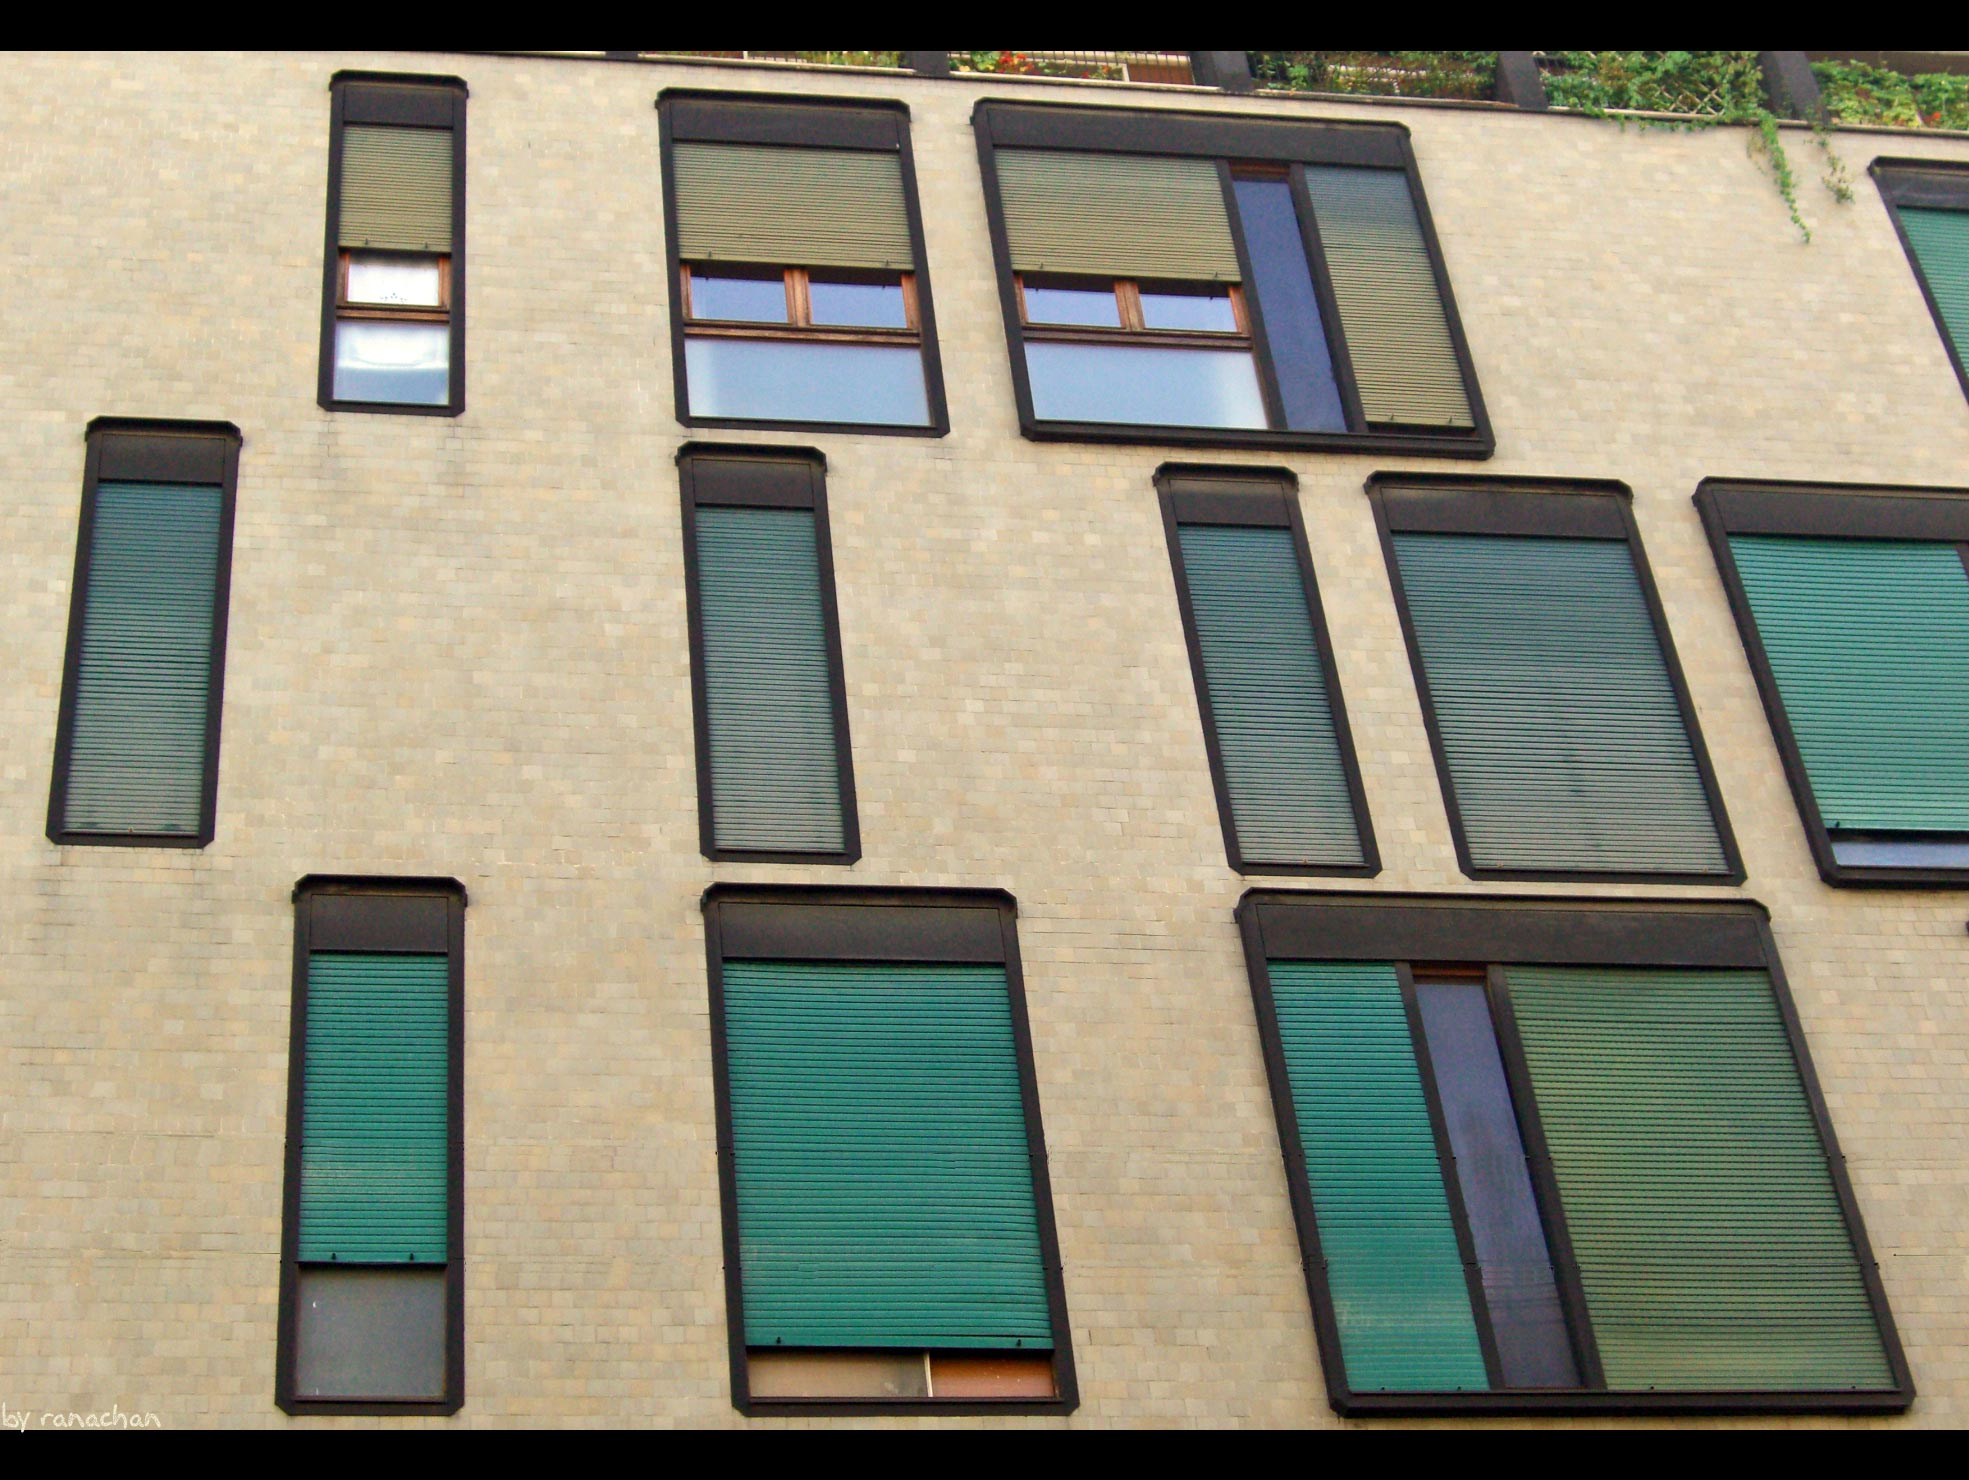
\includegraphics[width=0.95\textwidth]{window_geometry.jpg}
  \begin{center}
    {\large ``Window geometry''}\par
    Foto di midori.no.kerochan\par
    \url{http://www.flickr.com/photos/28661972@N05/2751042868/}\par
    Licenza: Creative Commons Attribution 2.0\par
  \end{center}
\newpage


\section{Estensione superficiale}\label{sect:estensione_superficiale}

Il \emph{tangram}\label{tangram} è un antichissimo gioco cinese. Il nome con cui lo conosciamo si pensa derivato dall'unione della parola \emph{tang} o \emph{tan}, che significa \emph{cinese}, e \emph{gram} che significa \emph{immagine}. Anticamente in Cina era chiamato ``schema intelligente a sette pezzi'' o anche ``le sette pietre della saggezza'' poiché si riteneva che la padronanza del gioco fosse la chiave per ottenere saggezza e talento.
Il gioco è costituito da un quadrato ritagliato in 7~pezzi poligonali aventi in comune solo punti del loro contorno (figura~\ref{fig:tangram}).

\begin{figure}[!htb]
	\centering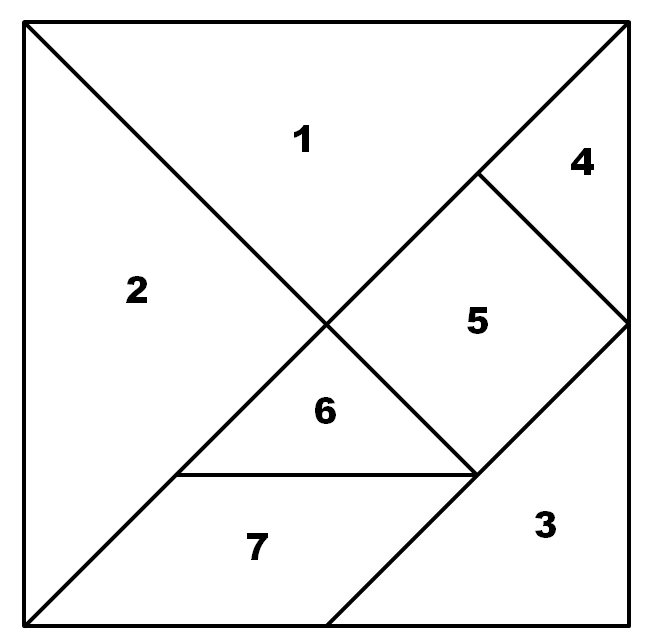
\includegraphics[width=0.6\textwidth]{tangram.png}
	\caption{Il gioco del tangram}\label{fig:tangram}
\end{figure}

I pezzi possono essere disposti e accostati gli uni agli altri senza sovrapposizioni in modo da ottenere una grande varietà di figure; la regola base è che devono essere utilizzati tutti i 7~pezzi. Si possono così formare alcuni disegni come mostrato nella figura~\ref{fig:figure_tangram}.

\begin{figure}[!htb]
	\centering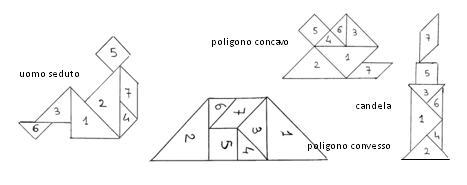
\includegraphics[width=0.8\textwidth]{figure_tangram.png}
	\caption{Alcune figure realizzabili con il tangram}\label{fig:figure_tangram}
\end{figure}

Potete osservare che si forma un poligono quando i singoli pezzi vengono accostati mediante un lato: l'uomo seduto è un poligono, ma non la candela; i due poligoni rappresentati sono l'uno concavo e l'altro convesso.

Con tutti i 7~pezzi del gioco si possono costruire 13~poligoni convessi, compreso il quadrato iniziale, provate a costruirli: fotocopiate la pagina precedente e ritagliate i 7~pezzi del tangram.

Evidentemente i 13~poligoni che avrete costruito non sono congruenti, né hanno la stessa forma; potete dire che sono formati dalle stesse parti poligonali, ciascuno può cioè essere pensato come unione dei \emph{tan} aventi in comune almeno un punto del loro perimetro, ma nessun punto interno.

\begin{definizione}
Con \emph{somma} di due \emph{figure piane} $X$ e $Y$, non aventi punti comuni o aventi in comune solo punti del loro contorno, intendiamo la figura $Z$ unione dei punti di $X$ e $Y$ e la indicheremo con
\begin{empheq}[box=\fbox]{equation*}
Z=X+Y
\end{empheq}
Diremo inoltre che $X$ è la \emph{differenza} tra $Z$ e $Y$ e scriveremo
\begin{empheq}[box=\fbox]{equation*}
X=Z-Y
\end{empheq}
\end{definizione}

\begin{definizione}
Due poligoni $p_1$ e $p_2$ sono \emph{equicomposti} se sono formati dalle stesse parti poligonali (figure piane). Sono \emph{equiscomponibili} se è possibile decomporre uno di essi in un numero finito di parti poligonali con le quali si possa ricoprire l'altro. In simboli
\begin{empheq}[box=\fbox]{equation*}
\vphantom{I}p_1 \doteq p_2
\end{empheq}
\noindent che si legge ``$p_1$ equicomposto $p_2$''
\end{definizione}

Tutte le figure poligonali costruite con i pezzi del tangram $p_1$, $p_2$, \ldots{} sono dunque poligoni equicomposti, ma possono anche essere considerati poligoni equiscomponibili, quindi $p_1 \doteq p_2 \doteq \ldots{}$

\begin{exrig}
\noindent\begin{minipage}{0.65\textwidth}\parindent15pt
\begin{esempio}\label{es:7.1}
Ritagliate da un quadrato i quattro triangoli rettangoli isosceli che si ottengono tracciando le sue diagonali (fotocopia e ritaglia la figura a fianco). Disponendo fianco a fianco i triangoli ottenuti in modo che i due lati comuni abbiano la stessa lunghezza, si ottengono 14~figure diverse. Due di esse sono riportate nella figura~\ref{fig:quadrato2}. Realizzate tutte le altre figure.
\end{esempio}
\end{minipage}\hfil
\begin{minipage}{0.35\textwidth}
	\centering% (c) 2014 Daniele Masini - d.masini.it@gmail.com
\begin{tikzpicture}[scale=1.2,font=\small]
\usetikzlibrary{calc}

\begin{scope}

\draw (0,0) -- (2,2);
\draw (0,2) -- (2,0);
\draw (0,0) -- (2,0) -- (2,2) -- (0,2) -- cycle;

\node at (0.4,1) {1};
\node at (1,1.6) {2};
\node at (1.6,1) {3};
\node at (1,0.4) {4};

\end{scope}

\end{tikzpicture}

\end{minipage}\vspace{5pt}

\begin{figure}[!htb]
\centering% (c) 2014 Daniele Masini - d.masini.it@gmail.com
\begin{tikzpicture}[scale=1.2,font=\small]
\usetikzlibrary{calc}

\begin{scope}

\draw (0,0) -- (4,0);
\draw (1,1) -- (5,1);
\draw (0,0) -- (1,1) -- (2,0) -- (3,1) -- (4,0) -- (5,1);

\end{scope}


\begin{scope}[xshift=6cm, yshift=0.5cm]

\draw (0,0) -- (2,0);
\draw (1,1) -- (3,1);
\draw (0,0) -- (1,1) -- (2,0) -- (3,1) -- (3,-1) -- (2,0) -- (1,-1) -- (3,-1);

\end{scope}

\end{tikzpicture}

\caption{Alcune figure realizzabili (esempio~\ref{es:7.1})}\label{fig:quadrato2}
\end{figure}

Le figure ottenute sono \ldots\ldots\ldots\ldots{} perché sono formate da \ldots\ldots\ldots\ldots{}

\noindent(da: Prova di allenamento della gara di ``Matematica senza frontiere'' del 9/02/1994)

\begin{esempio}\label{es:7.2}
Nella figura~\ref{fig:figure} sono disegnati un quadrato $ABCD$, un rettangolo $PQRS$ avente $PQ=2AB$ e $SP=AB/2$ e un rombo $FGHK$ avente una diagonale uguale al lato del quadrato e l'altra il doppio. Mostra come sia possibile scomporre ciascuno dei tre poligoni in parti tali da poter ricoprire gli altri due. Puoi concludere che i tre poligoni assegnati sono equiscomponibili? \ldots\ldots{}

\begin{figure}[!htb]
	\centering% (c) 2014 Daniele Masini - d.masini.it@gmail.com
\begin{tikzpicture}[scale=1.5,font=\small]
\usetikzlibrary{calc}

\begin{scope}
\draw (0,0) rectangle (1,1);
\node[shift={(-.2,-.2)}] at (0,0) {$A$};
\node[shift={(.2,-.2)}] at (1,0) {$D$};
\node[shift={(.2,.2)}] at (1,1) {$C$};
\node[shift={(-.2,.2)}] at (0,1) {$D$};
\end{scope}

\begin{scope}[xshift=2cm, yshift=0.25cm]
\draw (0,0) rectangle (2,0.5);
\node[shift={(-.2,-.2)}] at (0,0) {$P$};
\node[shift={(.2,-.2)}] at (2,0) {$Q$};
\node[shift={(.2,.2)}] at (2,0.5) {$R$};
\node[shift={(-.2,.2)}] at (0,0.5) {$S$};
\end{scope}

\begin{scope}[xshift=5cm, yshift=0.5cm]
\draw (0,0) node[shift={(-.2,0)}] {$F$} -- (1,-0.5) node[shift={(0,-.2)}] {$G$} -- (2,0) node[shift={(.2,0)}] {$H$} -- (1,0.5) node[shift={(0,.2)}] {$K$} -- cycle;
\end{scope}

\end{tikzpicture}

	\caption{Esempio~\ref{es:7.2}}\label{fig:figure}
\end{figure}

\end{esempio}

\noindent\begin{minipage}{0.6\textwidth}\parindent15pt
\begin{esempio}\label{es:7.3}
Dato l'insieme $F = \{f_1\text{,}f_2\text{,}f_3\}$ delle figure poligonali disegnate a lato, segui le seguenti istruzioni:\\
\verb|   |\textsl{ripeti:}\\
\verb|      |\textsl{scegli una figura dell'insieme $F$;}\\
\verb|      |\textsl{traccia alcuni segmenti che la decompongano in}\\
\verb|        |\textsl{parti poligonali;}\\
\verb|      |\textsl{forma con le parti ottenute altre 3 figure poligo-}\\
\verb|        |\textsl{nali;}\\
\verb|   |\textsl{finché non hai esaurito le figure.}\\
Costruisci l'insieme $G$ di tutti i poligoni ottenuti con questa procedura e indica con simboli arbitrari i suoi elementi.
\end{esempio}
\end{minipage}\hfil
\begin{minipage}{0.4\textwidth}
	\centering% Copyright (c) 2015 Daniele Masini - d.masini.it@gmail.com

\begin{tikzpicture}[scale=2,font=\small]
\usetikzlibrary{calc}

\begin{scope}
\draw (0,0) -- (1,0) -- (0.75,0.5) -- (-0.25,0.5) -- cycle;
\node at (0.4,0.25) {$f_1$};
\end{scope}

\begin{scope}[xshift=1.7cm]
\draw (0,0) -- (0.5,0.5) -- (-0.4,0.5) -- cycle;
\node at (0,0.3) {$f_2$};
\end{scope}

\begin{scope}[xshift=0.25cm, yshift=-1.1cm]
\draw (0,0) -- (1.5,0) -- (1,0.7) -- (0.25,0.5) -- cycle;
\node at (0.7,0.25) {$f_3$};
\end{scope}

\end{tikzpicture}

\end{minipage}\vspace{5pt}

\end{exrig}

Nell'insieme $S=F\cup G$ (dove $F$ e $G$ sono gli insiemi definiti nell'esempio~\ref{es:7.3}) la relazione $R$ espressa dal predicato: <<essere equicomposti>> gode della proprietà
\begin{itemize*}
\item riflessiva, infatti \ldots\ldots\ldots\ldots\ldots{}
\item simmetrica, infatti \ldots\ldots\ldots\ldots\ldots{}
\item transitiva, infatti \ldots\ldots\ldots\ldots\ldots{}
\end{itemize*}
Si può dunque concludere che $R$ è una relazione di equivalenza e quindi si possono costruire sia l'insieme delle parti $P(S)$, sia l'insieme quoziente $E=S/R$ avente come elementi le tre classi di equivalenza, ciascuna rappresentata dal poligono iniziale (figura~\ref{fig:insiemi}):
\[ [f_1] = \{x:x\text{ è un poligono equicomposto con }f_1\}; \]
\[ [f_2] = \{x:x\text{ è un poligono equicomposto con }f_2\}; \]
\[ [f_3] = \{x:x\text{ è un poligono equicomposto con }f_3\}. \]

\begin{figure}[!htb]
	\centering% Copyright (c) 2015 Daniele Masini - d.masini.it@gmail.com

\begin{tikzpicture}[scale=0.8,font=\small]
\usetikzlibrary{calc}

\begin{scope}
\draw (0,0) circle (2);
\draw[fill] (90:1.8) circle (1pt);
\draw[fill] (120:1.25) circle (1pt)  node[above] {$f_1$};
\draw[fill] (150:1.5) circle (1pt);
\draw[fill] (180:1.8) circle (1pt);
\draw (70:2) -- (190:2);
\draw[fill] (80:0.5) circle (1pt);
\draw[fill] (180:1) circle (1pt);
\draw[fill] (210:1.5) circle (1pt);
\draw[fill] (250:1.3) circle (1pt) node[above] {$f_2$};
\draw (70:2) -- (270:2);
\draw[fill] (300:1.2) circle (1pt);
\draw[fill] (330:1.3) circle (1pt);
\draw[fill] (40:1) circle (1pt);
\draw[fill] (10:1.5) circle (1pt) node[above] {$f_3$};
\node at (0,-2.5) {$P(S)$};
\end{scope}

\begin{scope}[xshift=5cm]
\draw (0,0) circle (2);
\draw[fill] (120:1) circle (1pt) node[above] {$[f_1]$};
\draw[fill] (250:1.3) circle (1pt) node[above] {$[f_2]$};
\draw[fill] (340:0.9) circle (1pt) node[above] {$[f_3]$};
\node at (0,-2.5) {$E$};
\end{scope}

\end{tikzpicture}

	\caption{Rappresentazione dell'insieme delle parti di $S$ e del quoziente $E=S/R$}\label{fig:insiemi}
\end{figure}

\begin{definizione}
Diciamo che due qualunque poligoni $p_1$ e $p_2$ appartenenti alla stessa classe sono \emph{equivalenti} e useremo la scrittura $p_1\doteq p_2$ per esprimere questa caratteristica (\emph{equivalenza per scomposizione}); essi hanno una caratteristica comune che chiamiamo \emph{estensione superficiale} (ES).
\end{definizione}

I poligoni costruiti con i pezzi del tangram appartengono alla stessa classe di equivalenza; essi sono dunque poligoni equivalenti e hanno la stessa estensione superficiale del quadrato iniziale.
Anche i 14~poligoni realizzati nell'esempio~\ref{es:7.1} appartengono alla stessa classe di equivalenza; essi sono dunque poligoni equivalenti e hanno la stessa estensione superficiale del quadrato assegnato.

\osservazione Sin dalla scuola elementare avete usato termini come ``superficie'', ``estensione'' e ``area'' quando vi siete accostati allo studio dei poligoni, probabilmente ritenendoli sinonimi. Lo studio di una particolare relazione di equivalenza vi ha mostrato che il concetto di estensione di un poligono si ottiene attraverso il procedimento di passaggio al quoziente nell'insieme dei poligoni piani.

\begin{definizione}
Chiamiamo \emph{area} di un poligono $p$ il numero reale positivo $A(p)$ che esprime la misura della sua estensione superficiale.
\end{definizione}

Possiamo concludere che ad ogni classe di equivalenza, generata con la relazione <<essere equicomposti>> o <<essere equiscomponibili>>, può essere associato un numero: l'area della figura scelta come rappresentante della classe di equivalenza. In tal modo trasformeremo una relazione di equivalenza tra poligoni, espressa con il simbolo $\doteq$ in una relazione di uguaglianza tra numeri.
Ad esempio, riferendoci ai poligoni costruiti con i pezzi del tangram possiamo trasformare la relazione di equivalenza $p_1\doteq p_2\doteq p_3\doteq \ldots{}$ in un'uguaglianza tra le aree scrivendo $A(p_1)=A(p_2)=A(p_3)=\ldots{}$

\section{Poligoni equivalenti}\label{sect:poligoni_equivalenti}

Premettiamo alcuni assiomi:
\nopagebreak
\begin{enumerate}
\item Poligoni congruenti sono equivalenti.
\item Un poligono non è equivalente ad una sua parte propria.
\item Somma e differenza di poligoni equivalenti originano poligoni equivalenti.
\end{enumerate}

\begin{teorema}\label{teo:7.1}
Due parallelogrammi aventi rispettivamente congruenti le basi e le rispettive altezze, sono equivalenti.
\end{teorema}

Nella figura sottostante sono rappresentati alcuni degli infiniti parallelogrammi aventi basi e altezze congruenti; le loro basi appartengono a rette parallele.

\noindent Ipotesi: $AB\cong EF\cong IJ$, $DM\perp AB$, $HN\perp EF$, $LO\perp IJ$, $DM\cong HN\cong LO$.\\
Tesi: $ABCD\doteq EFGH\doteq IJLK$.\\

\begin{figure*}[!htb]
	\centering% Copyright (c) 2015 Daniele Masini - d.masini.it@gmail.com

\begin{tikzpicture}[scale=1.2,font=\small]
\usetikzlibrary{calc}

\draw[dotted] (-0.5,0) -- (9,0);
\draw[dotted] (-0.5,1.5) -- (9,1.5);
\begin{scope}
\draw[thick, fill=red!10] (0,0) coordinate (a) node[shift={(-0.2,-0.2)}] {$A$} -- (1,0) coordinate (b) node[shift={(0.2,-0.2)}] {$B$} -- (1.3,1.5) coordinate (c) node[shift={(0.2,0.2)}] {$C$} -- (0.3,1.5) coordinate (d) node[shift={(-0.2,0.2)}] {$D$} -- cycle;
\draw[dashed, red] (d) -- ($(a)!(d)!(b)$) node[below, black] {$M$};
\draw[thick, blue] (a) -- (b);
\end{scope}

\begin{scope}[xshift=2.2cm]
\draw[thick, fill=red!10] (0,0) coordinate (e) node[shift={(-0.2,-0.2)}] {$E$} -- (1,0) coordinate (f) node[shift={(0.2,-0.2)}] {$F$} -- (2.4,1.5) coordinate (g) node[shift={(0.2,0.2)}] {$G$} -- (1.4,1.5) coordinate (h) node[shift={(-0.2,0.2)}] {$H$} -- cycle;
\draw[dashed, red] (h) -- ($(e)!(h)!(f)$) node[below, black] {$N$};
\draw[thick, blue] (e) -- (f);
\end{scope}

\begin{scope}[xshift=5cm]
\draw[thick, fill=red!10] (0,0) coordinate (i) node[shift={(-0.2,-0.2)}] {$I$} -- (1,0) coordinate (j) node[shift={(0.2,-0.2)}] {$J$} -- (3.4,1.5) coordinate (k) node[shift={(0.2,0.2)}] {$K$} -- (2.4,1.5) coordinate (l) node[shift={(-0.2,0.2)}] {$L$} -- cycle;
\draw[dashed, red] (l) -- ($(i)!(l)!(j)$) node[below, black] {$O$};
\draw[thick, blue] (i) -- (j);
\end{scope}

\end{tikzpicture}

\end{figure*}

\begin{proof}
Per dimostrare l'equivalenza tra questi parallelogrammi, costruiamo su $ABCD$ un altro parallelogramma, facendo sovrapporre le loro basi. Avremo tre casi:\\

\noindent\begin{minipage}{0.75\textwidth}\parindent15pt
\noindent\emph{Primo caso}\\
Costruiamo su $ABCD$ il parallelogramma $ABC'D'$ avente la stessa base $AB$ e la stessa altezza; il vertice $D'$ è un punto interno a $DC$. $ABCD$ è scomposto in $ADD' + ABCD'$; $ABC'D'$ è scomposto in $BCC' + ABCD'$. Se dimostriamo la congruenza dei triangoli $ADD'$ e $BCC'$ potremo concludere che i due parallelogrammi, essendo equicomposti, sono equivalenti.
Consideriamo i due triangoli $ADD'$ e $BCC'$, essi sono congruenti per il terzo criterio di congruenza, infatti: $AD\cong BC$ perché lati opposti del parallelogramma $ABCD$; $AD'\cong BC'$ perché lati opposti del parallelogramma $ABC'D'$; $DD'\cong CC'$ perché differenza di segmenti congruenti, precisamente $DD'=DC-D'C$ e $CC'=C'D'-CD'$. Dalla congruenza dei triangoli segue anche la loro equivalenza $ADD'\cong BCC' \:\Rightarrow\: ADD'\doteq BCC'$. Possiamo allora concludere che $ABCD\doteq ABC'D'$.\\
\end{minipage}\hfil
\begin{minipage}{0.25\textwidth}
	\centering% Copyright (c) 2015 Daniele Masini - d.masini.it@gmail.com

\begin{tikzpicture}[scale=1.2,font=\small]
\usetikzlibrary{calc}

\begin{scope}
\path[fill=blue!10, opacity=0.4] (0,0) coordinate (a) -- (1,0) coordinate (b) -- (1.3,2) coordinate (c) -- (0.3,2) coordinate (d) -- cycle;
\path[fill=red!10, opacity=0.4] (a) -- (b) -- (1.7,2) coordinate (c1) -- (0.7,2) coordinate (d1) -- cycle;
\draw[thick] (a) node[shift={(-0.2,-0.2)}] {$A$} -- (b) node[shift={(0.2,-0.2)}] {$B$} -- (c) node[shift={(0.2,0.2)}] {$C$} -- (d) node[shift={(-0.2,0.2)}] {$D$} -- cycle;
\draw[thick] (a) -- (b) -- (c1) node[shift={(0.2,0.2)}] {$C'$} -- (d1) node[shift={(-0.2,0.2)}] {$D'$} -- cycle;
\end{scope}

\end{tikzpicture}

\end{minipage}
\noindent\begin{minipage}{0.7\textwidth}\parindent15pt
\noindent\emph{Secondo caso}\\
Costruiamo su $ABCD$ il parallelogramma $ABC'D'$ avente la stessa base $AB$ e la stessa altezza; il vertice $C$ coincide con $D'$ e $ABCD$ è scomposto in $ADC + ACB$; $ABC'D'$ è scomposto in $ABD' + BC'D'$. Se dimostriamo la congruenza dei triangoli $ADC$ e $BC'D'$ possiamo concludere che i due parallelogrammi, essendo equicomposti, sono equivalenti. Infatti, $ADC$ e $BC'D'$ hanno $AD\cong CB$ perché lati opposti di uno stesso parallelogramma, $DC\cong C'D'$, $AC\cong BC'$, pertanto $ADC$ e $BC'D'$ sono triangoli congruenti.\\
\end{minipage}\hfil
\begin{minipage}{0.3\textwidth}
	\centering% (c) 2014 Daniele Masini - d.masini.it@gmail.com
\begin{tikzpicture}[scale=1.2,font=\small]
\usetikzlibrary{calc}

\begin{scope}
\path[fill=blue!10, opacity=0.4] (0,0) coordinate (a) -- (1,0) coordinate (b) -- (1.3,2) coordinate (c) -- (0.3,2) coordinate (d) -- cycle;
\path[fill=red!10, opacity=0.4] (a) -- (b) -- (2.3,2) coordinate (c1) -- (c) -- cycle;
\draw[thick] (a) node[shift={(-0.2,-0.2)}] {$A$} -- (b) node[shift={(0.2,-0.2)}] {$B$} -- (c) node[shift={(0,0.2)}] {$C\equiv D'$} -- (d) node[shift={(-0.2,0.2)}] {$D$} -- cycle;
\draw[thick] (a) -- (b) -- (c1) node[shift={(0.2,0.2)}] {$C'$} -- (c) -- cycle;
\end{scope}

\end{tikzpicture}

\end{minipage}
\noindent\begin{minipage}{0.65\textwidth}\parindent15pt
\noindent\emph{Terzo caso}\\
Costruiamo su $ABCD$ il parallelogramma $ABC'D'$ avente la stessa base $AB$ e la stessa altezza; il vertice $D'$ è esterno al lato $DC$ e i lati $AD'$ e $BC$ si intersecano nel punto $G$.
$ABCD$ è scomposto in $ADCG + AGB$ mentre $ABC'D'$ è scomposto in $BGD'C' + AGB$, inoltre $ADCG$ si può scomporre in $ADD' - CGD'$ come $BGD'C'$ si può scomporre in $BCC' - CGD'$.
Quindi $ABCD$ è scomposto in $ADD' - CGD' + AGB$ e $ABC'D'$ è scomposto in $BCC' - CGD' + AGB$.
Basta allora dimostrare la congruenza dei triangoli $ADD'$ e $BCC'$ per dire che $ABCD$ e $ABC'D'$ sono equiscomposti e dunque equivalenti. Infatti $ADD'$ e $BCC'$ sono congruenti perché hanno $AD\cong BC$, lati opposti del parallelogramma, analogamente $AD'\cong BC'$ e $DD'\cong CC'$ perché somma di segmenti congruenti.
\end{minipage}\hfil
\begin{minipage}{0.35\textwidth}
	\centering% (c) 2014 Daniele Masini - d.masini.it@gmail.com
\begin{tikzpicture}[scale=1.2,font=\small]
\usetikzlibrary{calc}

\begin{scope}
\path[fill=blue!10, opacity=0.4] (0,0) coordinate (a) -- (1,0) coordinate (b) -- (1.3,2) coordinate (c) -- (0.3,2) coordinate (d) -- cycle;
\path[fill=red!10, opacity=0.4] (a) -- (b) -- (3,2) coordinate (c1) -- (2,2) coordinate (d1) -- cycle;
\draw[thick] (a) -- (b) -- (c1) node[shift={(0.2,0.2)}] {$C'$} -- (d1) node[shift={(-0.2,0.2)}] {$D'$} -- cycle;
\draw[thick] (a) node[shift={(-0.2,-0.2)}] {$A$} -- (b) node[shift={(0.2,-0.2)}] {$B$} -- (c) node[shift={(0.2,0.2)}] {$C$} -- (d) node[shift={(-0.2,0.2)}] {$D$} -- cycle;

\draw[fill] (intersection of d1--a and c--b) circle (1pt) node[right] {$G$};
\draw[dotted] (c)-- (d1);
\end{scope}

\end{tikzpicture}

\end{minipage}
\end{proof}

\begin{corollario}\label{cor:7.1}
Ogni parallelogramma è equivalente al rettangolo avente un lato congruente alla sua base e l'altro lato congruente alla sua altezza.
\end{corollario}

\noindent Ipotesi: $AB\cong EF$, $CF\perp AB$, $CK\cong HE$.\\
Tesi: $ABCD\doteq EFGH$.

\begin{figure*}[!htb]
	\centering% Copyright (c) 2015 Daniele Masini - d.masini.it@gmail.com

\begin{tikzpicture}[scale=1.2,font=\small]
\usetikzlibrary{calc}

\begin{scope}
\draw[thick, fill=red!10] (0,0) coordinate (a) node[shift={(-0.2,-0.2)}] {$A$} -- (2,0) coordinate (b) node[shift={(0.2,-0.2)}] {$B$} -- (1.5,1.5) coordinate (c) node[shift={(0.2,0.2)}] {$C$} -- (-0.5,1.5) coordinate (d) node[shift={(-0.2,0.2)}] {$D$} -- cycle;
\draw[dashed, red] (c) -- ($(a)!(c)!(b)$) node[below, black] {$K$};
\draw[thick, blue] (a) -- (b);
\end{scope}

\begin{scope}[xshift=3.5cm]
\draw[thick, fill=red!10] (0,0) coordinate (e) node[shift={(-0.2,-0.2)}] {$E$} -- (2,0) coordinate (f) node[shift={(0.2,-0.2)}] {$F$} -- (2,1.5) coordinate (g) node[shift={(0.2,0.2)}] {$G$} -- (0,1.5) coordinate (h) node[shift={(-0.2,0.2)}] {$H$} -- cycle;
\draw[thick, red] (e) -- (h);
\draw[thick, blue] (e) -- (f);
\end{scope}

\end{tikzpicture}

\end{figure*}

\noindent\begin{minipage}{0.65\textwidth}\parindent15pt
\begin{proof}
Dal vertice $D$ tracciamo l'altezza $DL$ relativa alla base $AB$; il quadrilatero $DLKC$ è un rettangolo congruente a $EFGH$; dimostrando che $ABCD\doteq DLKC$ si ottiene la tesi.\\
Completate la dimostrazione.\\
Osserviamo che $ABCD$ è composto da \ldots\ldots\ldots\ldots{}
e $DLKC$ è composto da \ldots\ldots\ldots\ldots{} 
Consideriamo i triangoli \ldots\ldots\ldots\ldots{}
Sono congruenti perché \ldots\ldots\ldots\ldots{}
quindi \ldots\ldots\ldots\ldots{}
\end{proof}
\end{minipage}\hfil
\begin{minipage}{0.35\textwidth}
	\centering% (c) 2014 Daniele Masini - d.masini.it@gmail.com
\begin{tikzpicture}[scale=1.2,font=\small]
\usetikzlibrary{calc}

\begin{scope}
\path[fill=red!10, opacity=0.5] (0,0) coordinate (a) -- (2,0) coordinate (b) -- (1.5,1.5) coordinate (c) -- (-0.5,1.5) coordinate (d) -- cycle;
\draw[thick] (a) node[shift={(-0.2,-0.2)}] {$A$} -- (b) node[shift={(0.2,-0.2)}] {$B$} -- (c) node[shift={(0.2,0.2)}] {$C$} -- (d) node[shift={(-0.2,0.2)}] {$D$} -- cycle;
\node[below] at ($(a)!(c)!(b)$) {$K$};
\end{scope}

\begin{scope}[xshift=-.5cm]
\path[fill=red!10, opacity=0.5] (0,0) coordinate (e) -- (2,0) coordinate (f) -- (2,1.5) coordinate (g) -- (0,1.5) coordinate (h) -- cycle;
\draw[thick] (e) node[shift={(-0.2,-0.2)}] {$L$} -- (f) -- (g) -- (h) -- cycle;
\end{scope}

\end{tikzpicture}

\end{minipage}\vspace{5pt}

Il teorema~\ref{teo:7.1} e il suo corollario~\ref{cor:7.1} ci assicurano che i parallelogrammi aventi rispettivamente congruenti le basi e le relative altezze formano una classe di equivalenza avente come rappresentante il rettangolo che ha un lato congruente alla base del parallelogramma e l'altro lato congruente alla sua altezza. Possiamo quindi affermare che $ABCD\doteq EFGH \:\Rightarrow\: A_{ABCD} = A_{EFGH}$.

\begin{teorema}\label{teo:7.2}
Un triangolo è equivalente ad un parallelogramma avente:
\begin{enumeratea}
\item base congruente alla metà della base del triangolo e altezza congruente all'altezza del triangolo, oppure
\item base congruente alla base del triangolo e altezza congruente alla metà dell'altezza del triangolo.
\end{enumeratea}
\end{teorema}

Nella figura sono rappresentati il triangolo $ABC$, il parallelogramma $DEFG$ avente base congruente alla metà della base del triangolo e altezza congruente all'altezza del triangolo, il parallelogramma $IJLM$ avente altezza congruente alla metà dell'altezza del triangolo e base congruente alla base del triangolo.

\noindent Ipotesi: $AB\perp CH$, $DE\cong \frac{1}{2}AB$, $GK\perp DE$, $GK\cong CH$, $IJ\cong AB$, $MN\perp IJ$, $MN\cong \frac{1}{2}CH$.\\
Tesi: a) $ABC\doteq DEFG$;\quad b) $ABC\doteq IJLM$.

\begin{figure*}[!htb]
	\centering% (c) 2014 Daniele Masini - d.masini.it@gmail.com
\begin{tikzpicture}[scale=1.2,font=\small]
\usetikzlibrary{calc}

\begin{scope}
\draw[thick, fill=red!10] (0,0) coordinate (a) node[shift={(-0.2,-0.2)}] {$A$} -- (2,0) coordinate (b) node[shift={(0.2,-0.2)}] {$B$} -- (0.5,1.5) coordinate (c) node[shift={(0,0.2)}] {$C$} -- cycle;
\draw[dashed, red] (c) -- ($(a)!(c)!(b)$) node[below, black] {$H$};
\draw[thick, blue] (a) -- (b);
\end{scope}

\begin{scope}[xshift=3.5cm]
\draw[thick, fill=red!10] (0,0) coordinate (d) node[shift={(-0.2,-0.2)}] {$D$} -- (1,0) coordinate (e) node[shift={(0.2,-0.2)}] {$E$} -- (1.3,1.5) coordinate (f) node[shift={(0.2,0.2)}] {$F$} -- (0.3,1.5) coordinate (g) node[shift={(-0.2,0.2)}] {$G$} -- cycle;
\draw[dashed, red] (g) -- ($(d)!(g)!(e)$) node[below, black] {$K$};
\draw[thick, green!80!black] (d) -- (e);
\end{scope}

\begin{scope}[xshift=6cm]
\draw[thick, fill=red!10] (0,0) coordinate (i) node[shift={(-0.2,-0.2)}] {$I$} -- (2,0) coordinate (j) node[shift={(0.2,-0.2)}] {$J$} -- (2.3,0.75) coordinate (l) node[shift={(0.2,0.2)}] {$L$} -- (0.3,0.75) coordinate (m) node[shift={(-0.2,0.2)}] {$M$} -- cycle;
\draw[dashed, orange!70!black] (m) -- ($(i)!(m)!(j)$) node[below, black] {$N$};
\draw[thick, blue] (i) -- (j);
\end{scope}

\end{tikzpicture}

\end{figure*}

\begin{proof}~\vspace{4pt}\\
\noindent\begin{minipage}{0.65\textwidth}\parindent15pt
\noindent\emph{Caso a.}\\
Dal punto medio $T$ della base $AB$ tracciamo la parallela al lato $AC$ che incontra $CB$ in $S$; dal vertice $C$ tracciamo la parallela alla base $AB$ che interseca in $R$ la retta $ST$; il parallelogramma $ATRC$ soddisfa le ipotesi del caso a) ed è equivalente a $DEFG$ per il teorema~\ref{teo:7.1}.
Confrontiamo il triangolo e il parallelogramma: possiamo pensare $ABC$ composto da $CATS+BST$ e $ATRC$ composto da $CATS+CSR$.
Se dimostriamo la congruenza dei triangoli $CSR$ e $BST$ potremo concludere che triangolo e parallelogramma, essendo equicomposti, sono equivalenti. 
$TB\cong CR$ infatti \ldots\ldots\ldots\ldots{}
$SB\cong CS$ infatti \ldots\ldots\ldots\ldots{}
$T\widehat{B}S\cong S\widehat{C}R$ infatti \ldots\ldots\ldots\ldots{}
Allora per il primo criterio di congruenza $TBS\cong SCR$ e quindi $ATRC\doteq BST$.\\
\end{minipage}\hfil
\begin{minipage}{0.35\textwidth}
	\centering% (c) 2014 Daniele Masini - d.masini.it@gmail.com
\begin{tikzpicture}[scale=1.2,font=\small]
\usetikzlibrary{calc}

\begin{scope}
\draw[thick, fill=red!10] (0,0) coordinate (a) node[shift={(-0.2,-0.2)}] {$A$} -- (2,0) coordinate (b) node[shift={(0.2,-0.2)}] {$B$} -- (0.5,1.5) coordinate (c) node[shift={(0,0.2)}] {$C$} -- cycle;
%\draw[dashed, red] (c) -- ($(a)!(c)!(b)$) node[below, black] {$H$};
\draw (-0.1,1.5) coordinate (r1) -- (2.1,1.5) coordinate (r2);
\coordinate (t) at ($(a)!0.5!(b)$);
\coordinate (s) at ($(b)!0.5!(c)$);
\draw ($(t)!-0.3!(s)$) -- ($(t)!2.3!(s)$);
\coordinate (r) at (intersection of s--t and r1--r2);
\draw[fill] (r) circle (1pt) node[shift={(0.2,0.2)}] {$R$};
\draw[fill] (s) circle (1pt) node[shift={(0.2,0.2)}] {$S$};
\draw[fill] (t) circle (1pt) node[shift={(0.2,-0.2)}] {$T$};

\end{scope}

\end{tikzpicture}

\end{minipage}\vspace{1pt}
\noindent\begin{minipage}{0.65\textwidth}\parindent15pt
\noindent\emph{Caso b.}\\
Dal punto medio $V$ dell'altezza $CH$ tracciamo la parallela alla base $AB$ che interseca i lati $AC$ e $BC$ rispettivamente in $W$ e $Z$; da $B$ tracciamo la parallela al lato $AC$ che interseca la retta $WZ$ in $U$; il parallelogramma $AWUB$ soddisfa le ipotesi del caso b) ed è equivalente a $IJLM$ per il teorema~\ref{teo:7.1}.
Confrontiamo il triangolo e il parallelogramma: possiamo pensare $ABC$ composto da \ldots\ldots\ldots{} e $AWUB$ composto da \ldots\ldots\ldots{}
Se dimostriamo la congruenza dei triangoli $CWZ$ e $ZBU$ potremo concludere che triangolo e parallelogramma, essendo equicomposti, sono equivalenti.
$CW\cong \ldots{}$ infatti \ldots\ldots\ldots\ldots{}
$CZ\cong \ldots{}$ infatti \ldots\ldots\ldots\ldots{}
$\ldots{}\cong Z\widehat{B}U$ infatti \ldots\ldots\ldots\ldots{}
Pertanto \ldots\ldots\ldots\ldots{}
\end{minipage}\hfil
\begin{minipage}{0.35\textwidth}
	\centering% (c) 2014 Daniele Masini - d.masini.it@gmail.com
\begin{tikzpicture}[scale=1.2,font=\small]
\usetikzlibrary{calc}

\begin{scope}
\draw[thick, fill=red!10] (0,0) coordinate (a) node[shift={(-0.2,-0.2)}] {$A$} -- (2,0) coordinate (b) node[shift={(0.2,-0.2)}] {$B$} -- (0.5,1.5) coordinate (c) node[shift={(0,0.2)}] {$C$} -- cycle;
\draw[dashed] (c) -- ($(a)!(c)!(b)$) coordinate (h) node[below, black] {$H$};
\coordinate (t) at ($(a)!0.5!(b)$);
\coordinate (z) at ($(b)!0.5!(c)$);
\coordinate (w) at ($(a)!0.5!(c)$);
\path (b) -- +($(z)-(t)$) coordinate (b1);

\coordinate (u) at (intersection of w--z and b--b1);
\coordinate (v) at (intersection of c--h and w--z);

\draw ($(b)!-0.3!(u)$) -- ($(b)!1.3!(u)$);
\draw ($(w)!-0.3!(z)$) -- ($(w)!2.3!(z)$);

\draw[fill] (w) circle (1pt) node[shift={(-0.2,0.2)}] {$W$};
\draw[fill] (z) circle (1pt) node[shift={(0.2,0.2)}] {$Z$};
\draw[fill] (u) circle (1pt) node[shift={(-0.2,0.2)}] {$U$};
\draw[fill] (v) circle (1pt) node[shift={(0.2,0.2)}] {$V$};

\end{scope}

\end{tikzpicture}

\end{minipage}\vspace{1pt}
\end{proof}

\begin{corollario}\label{cor:7.2}
I triangoli aventi la stessa base e la stessa altezza sono equivalenti.
\end{corollario}

Lasciamo al lettore la dimostrazione di questa proprietà.

\begin{wrapfigure}{r}{0.6\textwidth}
	\centering% (c) 2014 Daniele Masini - d.masini.it@gmail.com
\begin{tikzpicture}[scale=1.2,font=\small]
\usetikzlibrary{calc}

\begin{scope}
\draw[thick, fill=red!10] (0,0) coordinate (a) node[shift={(-0.2,-0.2)}] {$A$} -- (1.3,0) coordinate (b) node[shift={(0.2,-0.2)}] {$B$} -- (1,1.5) coordinate (c) node[shift={(0,0.2)}] {$C$} -- cycle;
\draw[dashed] (c) -- ($(a)!(c)!(b)$) coordinate (l) node[below, black] {$L$};
\end{scope}

\begin{scope}[xshift=2.5cm]
\draw[thick, fill=red!10] (0,0) coordinate (d) node[shift={(-0.2,-0.2)}] {$D$} -- (1.3,0) coordinate (e) node[shift={(0.2,-0.2)}] {$E$} -- (1.3,0.75) coordinate (f) node[shift={(0.2,0.2)}] {$F$} -- (0,0.75) coordinate (g) node[shift={(-0.2,0.2)}] {$G$} -- cycle;
\end{scope}

\begin{scope}[xshift=5cm]
\draw[thick, fill=red!10] (0,0) coordinate (h) node[shift={(-0.2,-0.2)}] {$H$} -- (0.65,0) coordinate (i) node[shift={(0.2,-0.2)}] {$I$} -- (0.65,1.5) coordinate (j) node[shift={(0.2,0.2)}] {$J$} -- (0,1.5) coordinate (k) node[shift={(-0.2,0.2)}] {$K$} -- cycle;
\end{scope}


\end{tikzpicture}
\end{wrapfigure}
Il teorema~\ref{teo:7.2} e il suo corollario (\ref{cor:7.2}) ci assicurano che i triangoli aventi rispettivamente congruenti la base e la rispettiva altezza formano una classe di equivalenza avente come rappresentante il rettangolo con un lato congruente alla base del triangolo e l'altro lato congruente a metà della sua altezza, oppure un lato congruente all'altezza del triangolo e l'altro lato congruente a metà della base. 

\noindent Ipotesi: $CL\perp AB$, $DE\cong AB$, $DG\cong \frac{1}{2}CL$, $KH\cong CL$, $HI\cong\frac{1}{2}AB$.\\
Tesi: $ABC\doteq DEFG\doteq HIJK \:\Rightarrow\: A_{ABC}=A_{DEFG}=A_{HIJK}$.

\begin{teorema}\label{teo:7.3}
Un trapezio è equivalente a un triangolo avente per base la somma delle basi del trapezio e per altezza la stessa altezza.
\end{teorema}

\noindent Ipotesi: $EF\cong AB+CD$, $DH\perp AB$, $GI\perp EF$, $GI\cong DH$.\\
Tesi: $ABCD\doteq EFG$.

\begin{figure*}[!htb]
	\centering% (c) 2014 Daniele Masini - d.masini.it@gmail.com
\begin{tikzpicture}[scale=1.2,font=\small]
\usetikzlibrary{calc}

\begin{scope}[xshift=2.5cm]
\draw[thick, fill=red!10] (0,0) coordinate (a) node[shift={(-0.2,-0.2)}] {$A$} -- (1.7,0) coordinate (b) node[shift={(0.2,-0.2)}] {$B$} -- (1.3,1.5) coordinate (c) node[shift={(0.2,0.2)}] {$C$} -- (0.7,1.5) coordinate (d) node[shift={(-0.2,0.2)}] {$D$} -- cycle;
\draw[dashed, red] (d) -- ($(a)!(d)!(b)$) coordinate (h) node[below, black] {$H$};
\draw[thick, blue] (a) -- (b);
\draw[thick, green!80!black] (c) -- (d);
\end{scope}

\begin{scope}[xshift=6cm]
\draw[thick, fill=red!10] (0,0) coordinate (e) node[shift={(-0.2,-0.2)}] {$E$} -- (2.3,0) coordinate (f) node[shift={(0.2,-0.2)}] {$F$} -- (0.7,1.5) coordinate (g) node[shift={(0,0.2)}] {$G$} -- cycle;
\draw[dashed, red] (g) -- ($(e)!(g)!(f)$) coordinate (j) node[below, black] {$I$};

\draw[thick, blue] (e) -- +(0:1.7) coordinate (x);
\draw[thick, green!70!black] (x) -- (f);

\end{scope}

\end{tikzpicture}

\end{figure*}

\noindent\begin{minipage}{0.65\textwidth}\parindent15pt
\begin{proof}
Prolunghiamo la base $AB$ del segmento $BP$ congruente a $DC$ e congiungiamo $D$ con $P$.
$APD$ è un triangolo equivalente a $EFG$ avendo stessa base e stessa altezza, quindi basta dimostrare che $ABCD\doteq APD$.
Confrontiamo il trapezio e il triangolo: possiamo pensare 
$ABCD$ composto da \ldots\ldots\ldots\ldots{} 
e $APD$ composto da \ldots\ldots\ldots\ldots{}
Se dimostriamo la congruenza dei triangoli \ldots\ldots\ldots\ldots{}
potremo concludere che trapezio e triangolo, essendo equicomposti, sono equivalenti. 
I due triangoli sono congruenti perché hanno \ldots\ldots\ldots\ldots{} 
Possiamo quindi affermare che $ABCD\doteq APD \:\Rightarrow\: A_{ABCD}=A_{APD}$.
\end{proof}
\end{minipage}\hfil
\begin{minipage}{0.35\textwidth}
	\centering% Copyright (c) 2015 Daniele Masini - d.masini.it@gmail.com

\begin{tikzpicture}[scale=1.2,font=\small]
\usetikzlibrary{calc}

\begin{scope}[xshift=2.5cm]

\path[fill=red!10, opacity=0.5] (0,0) coordinate (a) -- (1.7,0) coordinate (b) -- (1.3,1.5) coordinate (c) -- (0.7,1.5) coordinate (d) -- cycle;

\path[fill=red!10, opacity=0.5] (0,0) coordinate (e) -- (2.3,0) coordinate (f) -- (0.7,1.5) coordinate (g) -- cycle;

\draw[thick] (a) node[shift={(-0.2,-0.2)}] {$A$} -- (b) node[shift={(0.2,-0.2)}] {$B$} -- (c) node[shift={(0.2,0.2)}] {$C$} -- (d) node[shift={(-0.2,0.2)}] {$D$} -- cycle;

\draw[thick] (e) -- (f) node[shift={(0.2,-0.2)}] {$P$} -- (g) -- cycle;

\draw[dashed, red] (d) -- ($(a)!(d)!(b)$) coordinate (h) node[below, black] {$H$};

\coordinate (q) at (intersection of f--g and b--c);
\draw[fill] (q) circle (1pt) node[right] {$Q$};

\end{scope}

\end{tikzpicture}

\end{minipage}\vspace{8pt}

Pertanto, utilizzando il teorema~\ref{teo:7.2} e il suo corollario (\ref{cor:7.2}) possiamo sempre determinare il rettangolo equivalente a un trapezio dato.

\begin{teorema}\label{teo:7.4}
Ogni poligono circoscritto ad una circonferenza è equivalente ad un triangolo avente per base il segmento somma dei lati del poligono e per altezza il raggio della circonferenza.
\end{teorema}

\noindent \emph{Caso del poligono regolare (pentagono).}\vspace{10pt}

\noindent Ipotesi: $LO\cong MN$, $AF\cong KG+GH+HI+IJ+LK$, $AB\cong KG$, $BC\cong GH$, $CD\cong HI$, $DE\cong IJ$, $EF\cong JK$.\\
Tesi : $KGHIJ\doteq AFM$.

\begin{figure*}[!htb]
	\centering% Copyright (c) 2015 Daniele Masini - d.masini.it@gmail.com

\begin{tikzpicture}[scale=0.7,font=\small]
\usetikzlibrary{calc}
\pgfmathsetmacro{\lati}{5}
\pgfmathsetmacro{\angoloc}{360/\lati}

\begin{scope}[rotate={\angoloc/2-90}]
%\clip (-2.1,-2.1) rectangle (2.5,2.1);
\coordinate (o) at (0,0);

\foreach \x/\y in {0/G,1/H,2/I,3/J,4/K}
{
	\path +({\x*\angoloc}:2) coordinate (\y) node [shift={({\x*\angoloc-45}:.2)}] {$\y$} -- ({(\x+1)*\angoloc}:2);
}
\draw[thick, blue, fill=red!10] (I) -- (J) -- (K) -- (G) -- (H) -- cycle; 
\draw[red] (o) circle(1.61);

\draw[fill] (o) circle (1.3pt) node[shift={(0.2,0.3)}] {$L$};

\draw[red, dashed] (o) -- node[black, midway, shift={(0.16,-0.1)}] {$a$} ({(4*\angoloc)+\angoloc/2}:2{*cos(\angoloc/2)}) coordinate (h) node[black, below] {$O$};
%\draw (o) let \p1 = ($(h)-(o)$) in circle ({veclen(\x1,\y1)});

\foreach \y in {I, J, K, G, H}
{
%	\node[shift={({\x*\angoloc-45}:.2)}] at (\y) {$\y$};
	\draw[dotted] (\y) -- (o);
}

\end{scope}

\begin{scope}[xshift=4cm, yshift=-1.618cm]
\path [fill=red!10] (0,0) coordinate(A) node[below] {$A$} let \p1 = ($(G)-(H)$) in -- ({5*veclen(\x1,\y1)},0) coordinate (F) node[below] {$F$} let \p2 = ($(h)-(o)$) in -- ({2.5*veclen(\x1,\y1)},{veclen(\x2,\y2)}) coordinate (m);

\foreach \a/\b in {1/B,2/C,3/D,4/E}
{
	\path[fill] let \p1 = ($(G)-(H)$) in ({\a*veclen(\x1,\y1)},0) circle (1.5pt) coordinate (\b) node [below] {$\b$};
   \draw[dotted] (\b) -- (m);
%	\draw[fill] ({\a*\x1}) circle (1pt) coordinate (\y) node [below] {$\y$};
}

\node[above] at (m) {$M$};
\draw[dashed, red] (m) -- ($(C)!(m)!(D)$) node[below, black] {$N$};
\draw[thick] (A) -- (m) -- (F) -- cycle;
\draw[thick, blue] (A) -- (F);
\end{scope}


\end{tikzpicture}

\end{figure*}

\begin{proof}
I cinque triangoli che compongono il triangolo $AFM$ sono equivalenti ai 5 triangoli che compongono il poligono assegnato, infatti hanno basi \ldots\ldots\ldots\ldots{} altezza \ldots\ldots\ldots\ldots{} 
Quindi \ldots\ldots\ldots\ldots{}
\end{proof}\vspace{10pt}

\noindent \emph{Caso del poligono qualunque.}\vspace{10pt}

\noindent Lasciamo al lettore la costruzione di un poligono circoscritto a una circonferenza e del triangolo equivalente.\vspace{10pt}

Possiamo quindi affermare che ogni poligono circoscritto a una circonferenza è equivalente ad un triangolo e per il teorema~\ref{teo:7.2} è anche equivalente a un rettangolo.

Si pone ora la questione: è possibile trasformare un qualunque poligono in un rettangolo equivalente?

\subsection{Costruzione di un rettangolo equivalente a un poligono assegnato}

\subsubsection{Caso 1: poligono convesso}
Un qualunque poligono convesso può essere trasformato in un poligono equivalente avente un lato di meno.

\begin{wrapfigure}{r}{0.4\textwidth}
	\centering% (c) 2014 Daniele Masini - d.masini.it@gmail.com
\begin{tikzpicture}[scale=1.35,font=\small]
\usetikzlibrary{calc}

\begin{scope}
\draw[thick, fill=red!10] (0,0) coordinate (a) node[shift={(-0.2,-0.2)}] {$A$} -- (1.2,1.5) coordinate (b) node[shift={(0,0.2)}] {$B$} -- (2,0.5) coordinate (c) node[shift={(0.2,0)}] {$C$} -- (1.7,-0.2) coordinate (d) node[shift={(0.2,-0.2)}] {$D$} -- cycle;
\draw[dashed] (a) -- (c);
\path (b) -- +($(c)-(a)$) coordinate (b1);
\draw[dashed] ($(b)!-0.5!(b1)$) node[above] {$b$} -- ($(b)!1!(b1)$);
\draw ($(d)!-0.5!(c)$) -- ($(d)!3.5!(c)$);
\coordinate (e) at (intersection of d--c and b--b1);
\draw (a) -- (e);
\draw[fill] (e) circle(1pt) node[shift={(0.2,-0.2)}] {$E$};
\end{scope}



\end{tikzpicture}
\end{wrapfigure}
\paragraph{Quadrilatero.}
In figura è rappresentato il quadrilatero convesso $ABCD$, ci proponiamo di costruire un triangolo equivalente ad esso. Dal vertice $B$ tracciamo la parallela $b$ alla diagonale $AC$; il vertice $E$ è il punto di intersezione di $b$ con la retta per $DC$. I triangoli $ABC$ e $ACE$ sono equivalenti in quanto hanno la stessa base $AC$ e stessa altezza, poiché i loro vertici si trovano sulla retta $b$ parallela alla base. Il quadrilatero $ABCD$ si può pensare composto da $ADC + ACB$; il triangolo $ADE$ è composto da \ldots\ldots\ldots{}; poiché sono poligono equicomposti possiamo concludere che $ABCD\doteq ADE$.

\begin{wrapfigure}{r}{0.4\textwidth}
	\centering% Copyright (c) 2015 Daniele Masini - d.masini.it@gmail.com

\begin{tikzpicture}[scale=1.5,font=\small]
\usetikzlibrary{calc}

\begin{scope}
\draw[thick, fill=red!10] (0,0) coordinate (a) node[shift={(-0.2,-0.2)}] {$A$} -- (1.5,0) coordinate (b) node[shift={(0.2,-0.2)}] {$B$} -- (2,0.75) coordinate (c) node[shift={(0.2,0)}] {$C$} -- (1,1.5) coordinate (d) node[shift={(0,0.2)}] {$D$} -- (0.1,0.75) coordinate (e) node[shift={(-0.2,0.2)}] {$E$} -- cycle;
\end{scope}

\end{tikzpicture}
\end{wrapfigure}
\paragraph{Pentagono.}
Costruzione di un triangolo equivalente al pentagono convesso $ABCDE$ rappresentato in figura.
Tracciare la diagonale $DB$.
Dal vertice $C$ tracciare la parallela a $DB$.
Prolungare il lato $AB$ fino a incontrare in $F$ la retta $r$.
Congiungere $D$ con $F$.
Si ha che  infatti \ldots\ldots\ldots{} 
Sul quadrilatero $FDE$ si può procedere come descritto precedentemente.

\paragraph*{}
Conclusione: ogni poligono convesso è equivalente a un triangolo e quindi (corollario~\ref{cor:7.2}) a un rettangolo.

\subsubsection{Caso 2: poligono concavo}

Premettiamo la costruzione di un triangolo con base assegnata equivalente ad un triangolo $ABC$ dato.

\begin{wrapfigure}{r}{0.4\textwidth}
	\centering% (c) 2014 Daniele Masini - d.masini.it@gmail.com
\begin{tikzpicture}[scale=1.2,font=\small]
\usetikzlibrary{calc}

\begin{scope}
\draw[thick, fill=red!10] (0,0) coordinate (a) node[shift={(-0.1,-0.2)}] {$A\equiv D$} -- (1,1.8) coordinate (b) node[shift={(0,0.2)}] {$B$} -- (2.7,0) coordinate (c) node[shift={(0.2,-0.2)}] {$C$} -- cycle;
\draw[thick] (c) -- (3.5,0) coordinate (e)  node[shift={(0.2,-0.2)}] {$E$};
\draw[dashed] (e) -- (b);
\path (c) -- +($(b)-(e)$) coordinate (c1);
\draw[dashed] (c) -- (c1);
\coordinate (m) at (intersection of c--c1 and a--b);
\draw[thick] (e) -- (m);
\draw[fill] (m) node[shift={(-0.25,-0.05)}] {$M$};
\end{scope}

\end{tikzpicture}
\end{wrapfigure}
Sia $ABC$ il triangolo e $DE$ il segmento che vogliamo come base del triangolo equivalente.
Sovrapponiamo il segmento $DE$ al lato $AC$ facendo coincidere $D$ con $A$; l'estremo $E$ è esterno al triangolo assegnato. Dopo aver congiunto $B$ con $E$, da $C$ tracciamo la parallela a $BE$ che incontra in $M$ il lato $AB$. Il triangolo $MDE$ è equivalente ad $ABC$.\\
Completate il ragionamento.\\
Si ha per costruzione: 
$DBE=ABC+BCE$ e $DBE=DME+BME$.
Quindi $ABC=DBE-BCE$ e $DME-BME$.
I triangoli $BCE$ e $BME$ sono equivalenti, avendo stessa base $BE$ e stessa altezza perché \ldots\ldots\ldots{}	Possiamo quindi concludere che \ldots\ldots\ldots{}

Passiamo ora alla costruzione di un rettangolo equivalente a un poligono concavo.

\begin{wrapfigure}{r}{0.55\textwidth}
	\centering% Copyright (c) 2015 Daniele Masini - d.masini.it@gmail.com

\begin{tikzpicture}[scale=1.4,font=\small]
\usetikzlibrary{calc}

\clip (-0.3,-0.3) rectangle (4.9,1.9);

\begin{scope}
\draw[thick, fill=red!10] (0,0) coordinate (a) node[shift={(-0.2,-0.2)}] {$A$} -- (0.8,1.5) coordinate (b) node[shift={(-0.1,0.2)}] {$B$} -- (1.7,0.9) coordinate (c) node[shift={(0,0.25)}] {$C$} -- (2.4,1.3) coordinate (d) node[shift={(0.2,0.2)}] {$D$} -- (2,0) coordinate (e) node[shift={(0.2,-0.2)}] {$E$} -- cycle;
\draw[dashed] (a) -- (c) -- (e);
\node at (0.9,0.8) {$T_1$};
\node at (1.3,0.3) {$T_2$};
\node at (2,0.7) {$T_3$};

\coordinate (c1) at ($(a)!(c)!(e)$);
\end{scope}

\begin{scope}[xshift = 3.4cm]
\coordinate (h) at (0,0);
\coordinate (k) at (1.2,0);

\coordinate (b1) at ($(a)!(b)!(c)$);
\path let \p1 = ($(c)-(a)$) in (h) -- +({veclen(\x1,\y1)},0) coordinate (z1);
\path let \p1=($(b)-(b1)$) in (z1) -- +(0,{veclen(\x1,\y1)/2}) coordinate (z2);
\path let \p1=(z2) in (h) -- +(0,{(\y1*\x1)/1.2cm}) coordinate (h1);
\path (h1) -- +(0:1.2) coordinate (k1);
%\draw (h) node[shift={(-0.2,-0.2)}] {$H$} -- (k) node[shift={(0.2,-0.2)}] {$K$} -- (k1) -- (h1) -- cycle;

\coordinate (c1) at ($(a)!(c)!(e)$);
\path let \p1 = ($(e)-(a)$) in (h) -- +({veclen(\x1,\y1)},0) coordinate (z1);
\path let \p1=($(c)-(c1)$) in (z1) -- +(0,{veclen(\x1,\y1)/2}) coordinate (z2);
\path let \p1=(z2) in (h1) -- +(0,{(\y1*\x1)/1.2cm}) coordinate (h2);
\path (h2) -- +(0:1.2) coordinate (k2);
%\draw (h1) -- (k1) -- (k2) -- (h2) -- cycle;

\coordinate (c2) at ($(e)!(c)!(d)$);
\path let \p1 = ($(d)-(e)$) in (h) -- +({veclen(\x1,\y1)},0) coordinate (z1);
\path let \p1=($(c)-(c2)$) in (z1) -- +(0,{veclen(\x1,\y1)/2}) coordinate (z2);
\path let \p1=(z2) in (h2) -- +(0,{(\y1*\x1)/1.2cm}) coordinate (h3);
\path (h3) -- +(0:1.2) coordinate (k3);
%\draw (h2) -- (k2) -- (k3) -- (h3) -- cycle;

\draw[thick, fill=red!10] (h) node[shift={(-0.2,-0.2)}] {$H$} -- (k) node[shift={(0.2,-0.2)}] {$K$} -- (k3) -- (h3) -- cycle;
\draw[dashed] (h1) -- (k1);
\draw[dashed] (h2) -- (k2);

\node at (0.6,0.35) {$R_1$};
\node at (0.6,1.1) {$R_2$};
\node at (0.6,1.65) {$R_3$};

\end{scope}

\end{tikzpicture}
\end{wrapfigure}
Dato il poligono concavo $ABCDE$, suddividiamolo in 3 triangoli tracciando due diagonali e fissiamo arbitrariamente un segmento $HK$. Ciascun triangolo in cui è suddiviso $ABCDE$ può essere trasformato in un triangolo equivalente avente $HK$ come base e dunque in un rettangolo con base $HK$; con tali rettangoli possiamo costruire, impilandoli uno sull'altro, il rettangolo equivalente ad $ABCDE$.

Possiamo quindi concludere che un qualunque poligono è equivalente a un rettangolo.

\subsection{Da un poligono al quadrato equivalente}

Nella classe di equivalenza di un qualsiasi poligono c'è sempre un quadrato. Ossia, dato un poligono possiamo sempre trovare un quadrato equivalente.
Abbiamo dimostrato che un qualunque poligono è equivalente a un rettangolo, ora vogliamo dimostrare che, dato un rettangolo esiste sempre un quadrato equivalente ad esso.
Vediamo due possibili costruzioni.

\begin{wrapfigure}{r}{0.35\textwidth}
	\centering% (c) 2014 Daniele Masini - d.masini.it@gmail.com
\begin{tikzpicture}[scale=1.2,font=\small]
\usetikzlibrary{calc, intersections}

\clip (-1.3,-0.3) rectangle (2.3,2.8);

\begin{scope}
\draw[thick, fill=red!10] (0,0) coordinate (a) node[shift={(-0.2,-0.2)}] {$A$} -- (2,0) coordinate (b) node[shift={(0.2,-0.2)}] {$B$} -- (2,0.75) coordinate (c) node[shift={(0.2,0.2)}] {$C$} -- (0,0.75) coordinate (d) node[shift={(-0.2,-0.2)}] {$D$} -- cycle;
\path[name path=Circle1] ($(c)!0.5!(d)$) circle (1);
\path[name path=rettaae] (0.75, 0.75) coordinate (e) -- (0.75,1.8);
\path [name intersections={of=Circle1 and rettaae}] ;
\path[fill] (intersection-1) coordinate (f);

\begin{scope}[yshift=0.75cm, rotate=52]
\draw[thick, fill=red!10] (0,0) -- (1.23,0) -- (1.23,1.23) node[shift={(0,.2)}] {$G$} -- (0,1.23) node[shift={(-.2,0)}] {$H$} -- cycle;
\end{scope}

\draw[fill] (f) circle (1pt) node[shift={(.2,.2)}] {$F$};
\draw[fill] (e) circle (1pt) node[shift={(.2,.2)}] {$E$};
\draw[dashed] (e) -- (f);

\begin{scope}
\clip (-0.1,0.75) -- (2.1,0.75) -- (2.1,1.77) -- (-0.1,1.77);
\draw ($(c)!0.5!(d)$) circle (1);
\end{scope}

\end{scope}

\end{tikzpicture}\vspace{6pt}\\
	\centering% (c) 2014 Daniele Masini - d.masini.it@gmail.com
\begin{tikzpicture}[scale=1.2,font=\small]
\usetikzlibrary{calc, intersections}

\clip (-0.3,-0.85) rectangle (2.85,1.55);

\begin{scope}
\draw[thick, fill=red!10] (0,-0.75) coordinate (a) node[left] {$A$} -- (2,-0.75) coordinate (b) node[right] {$B$} -- (2,0) coordinate (c)-- (0,0) coordinate (d) node[shift={(-.2,.2)}] {$D$} -- cycle;
\coordinate (e) at (0,0);
\draw (c) -- (2.75,0) coordinate (f);
\path[name path=rettag] (2, 0) coordinate (g) -- (2,1.5);
\path[name path=rettaj] (0.75, 0) coordinate (j) -- (0.75,1.5);
\path[name path=Circle1] ($(e)!0.5!(f)$) circle (1.375);

\path [name intersections={of=Circle1 and rettag}] ;
\path[fill] (intersection-1) coordinate (h);
\path [name intersections={of=Circle1 and rettaj}] ;
\path[fill] (intersection-1) coordinate (i);

\draw[thick, fill=red!10] (g) -- (h) -- (i) -- (j) -- cycle;

\draw[fill] (h) circle (1pt) node[shift={(.2,.2)}] {$G$};
\draw[fill] (i) circle (1pt) node[shift={(-.2,.2)}] {$H$};
\draw[fill] (j) circle (1pt) node[shift={(-.2,.2)}] {$I$};
\draw[fill] (c) circle (1pt) node[shift={(.2,.2)}] {$C$};
\draw[fill] (f) circle (1pt) node[below] {$E$};

\begin{scope}
\clip (-0.1,0) -- (2.8,0) -- (2.8,1.38) -- (-0.1,1.38);
\draw ($(e)!0.5!(f)$) circle (1.375);
\end{scope}

\end{scope}

\end{tikzpicture}\vspace{6pt}\\
	\centering% Copyright (c) 2015 Daniele Masini - d.masini.it@gmail.com

\begin{tikzpicture}[scale=1.2,font=\small]
\usetikzlibrary{calc, intersections}

\begin{scope}
\draw[thick, fill=red!10] (0,0) coordinate (a) node [shift={(-.2,-.2)}] {$A$} -- (0.6,1.5) coordinate (b) node [shift={(-.1,.2)}] {$B$} -- (1.7,0.9) coordinate (c) node [shift={(.1,.2)}] {$C$} -- (2.5,0.8) coordinate (d) node [shift={(.2,.2)}] {$D$} -- (2,0) coordinate (e) node [shift={(.2,-.2)}] {$E$} -- cycle;
\end{scope}

\end{tikzpicture}
\end{wrapfigure}
\paragraph{1\textsuperscript{o} modo}
Dopo aver disegnato il rettangolo $ABCD$ equivalente al poligono considerato, costruiamo la semicirconferenza di diametro $DC$. Fissiamo su $DC$ il punto $E$ tale che $DE\cong AD$. Dal punto $E$ tracciamo la perpendicolare al diametro che interseca la semicirconferenza in $F$. Il triangolo $DFE$ è retto in $E$ perché \ldots\ldots\ldots{}\\
Il quadrato avente come lato $DF$ è equivalente al rettangolo $ABCD$ perché \ldots\ldots\ldots{}

\paragraph{2\textsuperscript{o} modo}
Dato il rettangolo $ABCD$ equivalente al poligono considerato, prolunghiamone il lato $DC$ fino al punto $E$ tale che $CE\cong AD$. Quindi tracciamo la semicirconferenza di diametro $DE$. Dal punto $C$ tracciamo la perpendicolare al diametro che interseca la semicirconferenza in $G$. Il triangolo $DGE$ è retto in $G$ perché \ldots\ldots\ldots{}\\
Il quadrato avente come lato $CG$ è equivalente al rettangolo $ABCD$ perché \ldots\ldots\ldots{}

\paragraph*{}
Costruite il quadrato equivalente al poligono $ABCDE$ riportato nella figura a fianco.

\section{Aree dei principali poligoni}\label{sect:aree_poligoni}

Per \emph{area} di una qualunque figura piana intendiamo il numero reale che esprime la misura dell'estensione superficiale della figura data.

Per calcolare le aree dei principali poligoni si ricava per prima l'area del rettangolo e poi, basandosi sui teoremi relativi all'equivalenza delle figure piane, da questa si ricavano le aree di altri poligoni fondamentali.

\subsection{Area del rettangolo}

\begin{teorema}
L'area del rettangolo è data dal prodotto della misura delle sue dimensioni
\begin{empheq}[box=\fbox]{equation*}
A=b\cdot h
\end{empheq}
\end{teorema}

\begin{figure*}[!htb]
	\centering% Copyright (c) 2015 Daniele Masini - d.masini.it@gmail.com

\begin{tikzpicture}[scale=0.8,font=\small]
\usetikzlibrary{calc}

\begin{scope}
\draw[thick, fill=red!10] (0,0) -- node[below] {$b$} (3,0) -- node[right] {$h$} (3,2) -- (0,2) -- cycle;
\node at (1.5,1) {$R$};
\end{scope}

\begin{scope}[xshift=4.5cm]
\draw[thick, fill=blue!10] (0,0) -- node[below] {$u$} (1,0) -- node[right] {$h$} (1,2) -- (0,2) -- cycle;
\node at (0.5,1) {$R'$};
\end{scope}

\begin{scope}[xshift=7cm]
\draw[thick, fill=yellow!10] (0,0) -- node[below] {$u$} (1,0) -- node[right] {$u$} (1,1) -- (0,1) -- cycle;
\node at (0.5,0.5) {$Q$};
\end{scope}


\end{tikzpicture}
\end{figure*}

\begin{proof}
A questo scopo ricorriamo al teorema~\ref{teo:6.2} <<I rettangoli aventi una dimensione congruente sono direttamente proporzionali all'altra dimensione>>. Consideriamo allora un rettangolo $R$ le cui misure della base e dell'altezza sono rispettivamente $b$ e $h$, il rettangolo $R'$ che otteniamo da $R$ trasformando una dimensione, ad esempio la sua base, in quella unitaria $u$, di misura 1, ed infine il quadrato $Q$ di lato $u$.
Applichiamo il teorema enunciato in precedenza a $R$ ed a $R'$ ottenendo $R : R' = b : u$.
Quindi applichiamo lo stesso teorema al rettangolo $R'$ ed al quadrato unitario $Q$, così abbiamo $R' : Q = h : u$.
Passiamo dalla proporzione tra le grandezze alla proporzione tra le loro misure, iniziando dall'ultima proporzione e chiamando rispettivamente $A$ ed $A'$ le misure delle estensioni superficiali di $R$ ed $R'$. Si ha $A' : 1 = h : 1$, da cui ricaviamo $A' = h$.
Sostituiamo dunque nella prima proporzione le misure di $R'$, $b$ e $u$, si ha $A : A' = b : 1 \:\Rightarrow\: A : h = b : 1$, da cui ricaviamo $A=b\cdot h$
che è proprio ciò che volevamo dimostrare.
\end{proof}

\subsection{Area del quadrato}

Poiché il quadrato è un particolare rettangolo avente le dimensioni congruenti tra loro, $b = h = l$, anche la sua area si calcolerà in modo analogo a quella del rettangolo $A=b\cdot h=l\cdot l$ ovvero
\begin{empheq}[box=\fbox]{equation*}
A=l^2
\end{empheq}
Dunque l'area del quadrato è data dal quadrato del lato.

\subsection{Area del parallelogramma}

\begin{wrapfigure}{r}{0.3\textwidth}
	\centering% (c) 2014 Daniele Masini - d.masini.it@gmail.com
\begin{tikzpicture}[scale=1,font=\small]
\usetikzlibrary{calc}

\begin{scope}
\draw[thick, fill=red!10] (0,0) coordinate (a) -- node [below] {$b$} (2,0) coordinate (b) -- (2.5,1.5) -- (0.5,1.5) coordinate (d) -- cycle;
\draw[dashed] (d) -- node[right] {$h$} ($(a)!(d)!(b)$);
\end{scope}

\end{tikzpicture}

\end{wrapfigure}
Ricordando il teorema~\ref{teo:7.1} sull'equivalenza tra parallelogrammi, secondo il quale due parallelogrammi sono equivalenti quando hanno un lato (base) e l'altezza ad esso relativa tra loro congruenti, da cui deriva il corollario~\ref{cor:7.1} che un parallelogramma è equivalente ad un rettangolo avente base ed altezza congruenti a quelle del parallelogramma stesso, è immediato dedurre che anche l'area del parallelogramma si calcola moltiplicando un lato, ritenuto la base, per l'altezza ad esso relativa, cioè
\begin{empheq}[box=\fbox]{equation*}
A=b\cdot h
\end{empheq}

\subsection{Area del triangolo}

Anche in questo caso ci si deve rifare al teorema~\ref{teo:7.2} sull'equivalenza tra un triangolo e un parallelogramma <<Un triangolo è equivalente ad un parallelogramma avente come base metà della base del triangolo ed altezza congruente a quella del triangolo>>. Appare allora evidente che l'area del triangolo è
\begin{empheq}[box=\fbox]{equation*}
A=\dfrac{b}{2}\cdot h
\end{empheq}
dove $b/2$ è la base del parallelogramma ad esso equivalente.

\subsection{Area del trapezio}

Sempre dai teoremi sull'equivalenza, sappiamo che <<Un trapezio è equivalente ad un triangolo la cui base è congruente alla somma delle basi del trapezio e la cui altezza ad essa relativa è congruente all'altezza del trapezio>> (teorema~\ref{teo:7.3}). Dunque l'area del trapezio sarà
\begin{empheq}[box=\fbox]{equation*}
A=\dfrac{B+b}{2}\cdot h
\end{empheq}
dove $B + b$ è la somma delle basi del trapezio, e quindi $(B + b)/2$ è la base del triangolo ad esso equivalente.

\subsection{Area del rombo}

\begin{wrapfigure}{r}{0.4\textwidth}
	\centering% (c) 2014 Daniele Masini - d.masini.it@gmail.com
\begin{tikzpicture}[scale=0.8,font=\small]
\usetikzlibrary{calc}

\begin{scope}
\draw[thick, fill=red!10] (0,0) coordinate (a) -- node [below] {$l$} ++(0:2) coordinate (b) -- node[right] {$l$} ++(60:2) -- ++(180:2) coordinate (d) -- cycle;
\draw[dashed] (d) -- node[right] {$h$} ($(a)!(d)!(b)$);
\end{scope}

\begin{scope}[xshift=5cm]
\draw[dotted] (-1,0) rectangle (1,{sqrt(3)*2});

\begin{scope}[rotate=60]
\draw[thick, fill=red!10] (0,0) coordinate (a) -- ++(0:2) coordinate (b) -- ++(60:2) coordinate (c) -- ++(180:2) coordinate (d) -- cycle;
\draw[dashed] (a) -- node[right, shift={(-0.05,0.5)}] {$D$} (c);
\draw[dashed] (b) -- node[above, shift={(-0.4,-0.05)}] {$d$} (d);
\end{scope}
\end{scope}

\end{tikzpicture}

\end{wrapfigure}
Poiché il rombo è un particolare parallelogramma, la sua area si trova moltiplicando uno dei suoi lati per l'altezza ad esso relativa, cioè $A=l\cdot h$.
Possiamo però notare che un rombo si può considerare come la metà di un rettangolo le cui dimensioni sono congruenti alle diagonali del rombo ($D$ e $d$).
Come si può facilmente dimostrare, le due diagonali dividono il rombo in quattro triangoli rettangoli congruenti ai quattro triangoli rettangoli esterni al rombo, e quindi il rombo è equivalente alla metà del rettangolo, per cui la sua area può essere espressa come
\begin{empheq}[box=\fbox]{equation*}
A=\dfrac{D\cdot d}{2}
\end{empheq}

Si può inoltre dimostrare, in maniera del tutto analoga a quanto precedentemente descritto, che l'area di un qualsiasi quadrilatero che abbia le diagonali perpendicolari è determinabile in questo modo.

\subsection{Area di un poligono circoscrivibile ad una circonferenza}

Ricordiamo anche in questo caso il teorema~\ref{teo:7.4} <<un poligono circoscrivibile ad una circonferenza è equivalente ad un triangolo che ha per base il perimetro del poligono e per altezza il raggio della circonferenza inscritta>>.
Da qui segue immediatamente che l'area di questo tipo di poligono è data da
\begin{empheq}[box=\fbox]{equation*}
A=\dfrac{2p\cdot r}{2}=p\cdot r
\end{empheq}
dove, come di consuetudine, $p$ indica il semiperimetro.

In particolare, se il poligono è regolare, sarà sempre possibile calcolare l'area per mezzo della formula
\begin{empheq}[box=\fbox]{equation*}
A=p\cdot a
\end{empheq}
dove $a$ è l'apotema, cioè il raggio della circonferenza inscritta nel poligono regolare.

\section{Teoremi di Pitagora e di Euclide}\label{sect:teoremi_pitagora_euclide}

\begin{teorema}[Primo teorema di Euclide]
In un triangolo rettangolo, il quadrato costruito su un cateto è equivalente al rettangolo che ha come dimensioni l'ipotenusa e la proiezione del cateto stesso sull'ipotenusa.
\end{teorema}


\noindent\begin{minipage}{0.63\textwidth}\parindent15pt
\begin{proof}
Sia $ABC$ un triangolo rettangolo in $B$. Tracciamo l'altezza $BH$ relativa all'ipotenusa $AC$ e prolunghiamola di un segmento $HD$ congruente all'ipotenusa stessa e costruiamo il rettangolo $AEDH$. Sul cateto $AB$ costruiamo il quadrato $ABGF$. Prolunghiamo i lati $HD$ ed $AE$ del rettangolo ed il lato $FG$ del quadrato e chiamiamo $I$ e $J$ i punti di intersezione tra questi prolungamenti. Otteniamo il parallelogramma $ABJI$.
La tesi da dimostrare è che il quadrato $ABGF$ è equivalente al rettangolo $AEDH$.

Consideriamo innanzitutto i triangoli $AIF$ e $ABC$, essi sono congruenti in quanto hanno entrambi un angolo retto ($A\widehat{F}I$ e $A\widehat{B}C$), $AF\cong AB$ in quanto lati di un quadrato, $F\widehat{A}I\cong B\widehat{A}C$ in quanto complementari dello stesso angolo $I\widehat{A}B$.
Dunque i due triangoli sono congruenti per il secondo criterio generalizzato, ed in particolare avranno $AI\cong AC$.

Consideriamo ora il parallelogramma $ABJI$ ed il quadrato $ABGF$; essi sono equivalenti in quanto hanno il lato $AB$ in comune e la stessa altezza $BG$ relativa a questo lato. 
Consideriamo poi il parallelogramma $ABJI$ ed il rettangolo $AHDE$; anch'essi sono equivalenti poiché hanno basi congruenti $AE$ e $AI$, entrambe congruenti ad $AC$, e stessa altezza $AH$.
Allora per la proprietà transitiva dell'equivalenza avremo che anche il quadrato $ABGF$ è equivalente al rettangolo $AEDH$ e così la tesi è provata.
\end{proof}
\end{minipage}\hfil
\begin{minipage}{0.37\textwidth}
	\centering% (c) 2014 Daniele Masini - d.masini.it@gmail.com
\begin{tikzpicture}[scale=0.9,font=\small]
\usetikzlibrary{calc}

%\begin{scope}[rotate=121]
\begin{scope}[rotate=-121]
\path[fill=red!10] (0,0) coordinate (a) -- (-1.5,0) coordinate (b) -- (-1.5,2.5) coordinate (c) -- cycle;
\draw[green!70!black, fill=green!10] (b) rectangle +(0.3,0.3);
\draw[fill=blue!10] (a) let \p1=(b) in -- (b) -- (\x1,\x1) coordinate (g) node[above left] {$G$} -- (0,\x1) coordinate (f) node [left] {$F$} -- cycle;
\end{scope}
\draw (b) -- ($(a)!(b)!(c)$) coordinate (h);
\draw[fill=blue!10] (a) let \p1=(c) in -- (0,{-\x1}) coordinate (e) node[below left] {$E$} let \p2=(h) in -- +({\x2},0) coordinate (d) node[below right] {$D$} -- (h) -- cycle;
\begin{scope}
\clip (a) let \p1=(c) in -- ({\x1+0.1},0) -- ({\x1},{-\x1}) -- (0,{-\x1}) -- cycle;
\draw[dotted] (a) let \p1=(c) in circle ({\x1});
\end{scope}

\draw[thick] (a) node[left] {$A$} -- (b) node [above right]{$B$} -- (c) node[right] {$C$} -- cycle;

\path (a) -- (0,1) coordinate (a1);
\coordinate (i) at (intersection of a--a1 and f--g);
\coordinate (j) at (intersection of h--b and f--g);
\draw (g) -- (j);
\draw (a) -- (i);
\draw (b) -- (j);

\draw[fill] (h) circle (1.2pt) node[below right] {$H$};
\draw[fill] (i) circle (1.2pt) node[above left] {$I$};
\draw[fill] (j) circle (1.2pt) node[above] {$J$};
%\end{scope}

\end{tikzpicture}

\end{minipage}\vspace{8pt}

Vale anche il teorema inverso.
\begin{teorema}[Primo teorema di Euclide {[}inverso{]}]
Se in un triangolo il quadrato costruito su un lato è equivalente al rettangolo che ha per dimensioni il lato maggiore del triangolo e la proiezione del primo lato su di esso, allora il triangolo è rettangolo.
\end{teorema}

\begin{proof}
Per la dimostrazione si usa la stessa costruzione fatta per il teorema diretto. Si inizia dimostrando nello stesso modo l'equivalenza tra il quadrato $ABGF$ ed il parallelogramma $ABJI$. Poiché per ipotesi il rettangolo $AHDE$ è equivalente al quadrato $ABGF$, allora per la proprietà transitiva dell'equivalenza avremo che il rettangolo $AHDE$ ed il parallelogramma $ABJI$ sono equivalenti. Poiché parallelogramma e rettangolo hanno la stessa altezza $AH$, essendo equivalenti dovranno avere congruenti le basi $HD\cong BJ$. Ma per costruzione $HD\cong AC$, e quindi sarà anche $BJ\cong AC$, da cui segue $AI\cong BJ\cong AC$. Quindi i triangoli $AIF$ ed $ABC$ saranno congruenti per il primo criterio in quanto hanno $AI\cong AC$ e $AB\cong AF$, poiché lati di un quadrato, e $F\widehat{A}I\cong B\widehat{A}C$ in quanto complementari dello stesso angolo $I\widehat{A}B$. Dunque avranno anche gli angoli $A\widehat{F}I\cong A\widehat{B}C$ e poiché $A\widehat{F}I$ è retto lo sarà anche $A\widehat{B}C$.
\end{proof}

\begin{teorema}[di Pitagora]
In un triangolo rettangolo il quadrato costruito sull'ipotenusa è equivalente alla somma dei quadrati costruiti sui cateti.
\end{teorema}

\noindent\begin{minipage}{0.55\textwidth}\parindent15pt
\begin{proof}
Dopo aver disegnato i quadrati $Q_1$ e $Q_2$ sui cateti e $Q$ sull'ipotenusa del triangolo rettangolo $ABC$, tracciamo l'altezza $BH$ relativa all'ipotenusa $AC$ e prolunghiamola finché non incontra il lato $IE$ del quadrato $Q$, il quale risulta così diviso in due rettangoli $R_1$ ed $R_2$.
Applicando il primo teorema di Euclide al triangolo rettangolo $ABC$ avremo che $Q_1\doteq R_1$ e che $Q_2\doteq R_2$ in quanto, per costruzione, $R_1$ ed $R_2$ hanno la stessa altezza, pari alla lunghezza dell'ipotenusa $AC$ e ognuno di essi ha la base pari alla proiezione sull'ipotenusa stessa del relativo cateto. Sommando quindi ambo i membri di queste due equivalenze otteniamo che $Q_1+Q_2\doteq R_1+R_2$. Ma $R_1+R_2\doteq Q$, da cui segue, per la proprietà transitiva dell'equivalenza, $Q\doteq Q_1+Q_2$, che è proprio quanto volevamo dimostrare.
\end{proof}
\end{minipage}\hfil
\begin{minipage}{0.45\textwidth}
	\centering% Copyright (c) 2015 Daniele Masini - d.masini.it@gmail.com

\begin{tikzpicture}[scale=0.9,font=\small]
\usetikzlibrary{calc}

%\begin{scope}[rotate=121]
\begin{scope}[rotate=-121]
\path[fill=red!10] (0,0) coordinate (a) -- (-1.5,0) coordinate (b) -- (-1.5,2.5) coordinate (c) -- cycle;
\draw[gray!70!black, fill=gray!10] (b) rectangle +(0.3,0.3);
\draw[fill=green!10] (a) let \p1=(b) in -- (b) -- (\x1,\x1) coordinate (g) node[above] {$G$} -- (0,\x1) coordinate (f) node [left] {$F$} -- cycle;
\draw[fill=blue!10] (b) let \p1=($(c)-(b)$) in -- (c) -- ++(-\y1,0) coordinate (k) node[right] {$K$} -- ++(0,-\y1) coordinate (j) node [above] {$J$} -- cycle;
\path (f) -- node {$Q_1$} (b);
\path (c) -- node {$Q_2$} (j);
\end{scope}
\coordinate (h) at ($(a)!(b)!(c)$);
\path[fill=green!10] (a) let \p1=(c) in -- (0,{-\x1}) coordinate (e) node[below left] {$E$} let \p2=(h) in -- +({\x2},0) coordinate (d) -- (h) -- cycle;
\path[fill=blue!10] (h) -- (c) let \p1=(c) in -- +(0,{-\x1}) coordinate (i) -- (d) -- cycle;

\draw (a) -- (e) node[below left] {$E$} -- (i) node[below right] {$I$} -- (c) -- cycle;
\draw[dashed] (b) -- (d);
\path (a) -- node {$R_1$} (d);
\path (d) -- node {$R_2$} (c);
\path (a) -- node[shift={(0,-0.7)}] {$Q$} (i);

\draw[thick] (a) node[left] {$A$} -- (b) node [above]{$B$} -- (c) node[right] {$C$} -- cycle;

\draw[fill] (h) circle (1.2pt) node[below right] {$H$};
\draw[fill] (d) circle (1.2pt) node[below] {$D$};
%\end{scope}

\end{tikzpicture}

\end{minipage}\vspace{8pt}

Anche per il teorema di Pitagora vale il teorema inverso.

\begin{teorema}[di Pitagora {[}inverso{]}]
Se in un triangolo il quadrato costruito su un lato  è equivalente alla somma dei quadrati costruiti sugli altri due lati, allora il triangolo è rettangolo.
\end{teorema}

\begin{proof}
Sia $ABC$ il triangolo per cui vale il teorema di Pitagora; vogliamo dimostrare che questo triangolo è rettangolo.
Consideriamo il triangolo rettangolo $A'B'C'$, i cui cateti $A'B'$ e $A'C'$ siano rispettivamente congruenti ai due lati del triangolo $AB$ e $AC$. Al triangolo $A'B'C'$ possiamo applicare il teorema di Pitagora, per cui abbiamo che il quadrato costruito su $B'C'$ è equivalente alla somma dei quadrati costruiti sui cateti $A'B'$ e $A'C'$. I quadrati costruiti sui lati congruenti $AB$ e $A'B'$ sono congruenti, così come lo sono i quadrati costruiti su $AC$ e $A'C'$, quindi avremo che: $Q_{AB} + Q_{AC} \doteq Q_{A'B'} + Q_{A'C'}$. Poiché per ipotesi $Q_{AB} + Q_{AC} \doteq Q_{BC}$ e, avendo applicato il teorema di Pitagora al triangolo $A'B'C'$, sarà anche $Q_{A'B'} + Q_{A'C'} \doteq Q_{B'C'}$. Per la proprietà transitiva dell'equivalenza avremo che: $Q_{BC} \doteq Q_{B'C'}$. Poiché due quadrati sono equivalenti quando hanno lo stesso lato, avremo che $BC\cong B'C'$, e quindi i due triangoli sono congruenti per il terzo criterio. Allora saranno congruenti anche gli angoli $\widehat{A}$ e $\widehat{A'}$, e poiché $\widehat{A'}$ è retto, lo sarà anche $\widehat{A}$. Quindi $ABC$ è un triangolo rettangolo.
\end{proof}

\begin{teorema}[Secondo teorema di Euclide]
In un triangolo rettangolo, il quadrato costruito sull'altezza relativa all'ipotenusa è equivalente al rettangolo che ha per dimensioni le proiezioni dei cateti sull'ipotenusa.
\end{teorema}

\noindent\begin{minipage}{0.6\textwidth}\parindent15pt
\begin{proof}
Dobbiamo dimostrare che il quadrato $Q$ che ha come lato l'altezza relativa all'ipotenusa è equivalente al rettangolo $R_1$ che ha come lati le due proiezioni dei cateti sull'ipotenusa.

La costruzione è la seguente: dopo aver disegnato il quadrato $Q$ si disegnano anche il quadrato $Q_1$, che ha come lato il cateto $AB$, ed il rettangolo $R$, che ha come lati l'ipotenusa e la proiezione $AH$ di $AB$ sull'ipotenusa. All'interno di questo rettangolo possiamo individuare il quadrato $Q_2$, di lato $AH$, ed il rettangolo $R_1$, che ha come dimensioni $NM\cong AH$ e $MD\cong HD-HM\cong HC$, in quanto $HD\cong AC$ e $HM\cong AH$.

Consideriamo ora il triangolo rettangolo $ABH$, e applichiamo ad esso il teorema di Pitagora, risulta $Q_1\doteq Q+Q_2$. Applichiamo ora al triangolo $ABC$ il primo teorema di Euclide, si ha $Q_1\doteq R$. Confrontiamo le due relazioni ed applichiamo la proprietà transitiva dell'equivalenza $Q+Q_2\doteq R$. Ma $R\doteq Q_2 + R_1$, quindi sostituendo avremo $Q+Q_2\doteq Q_2 + R_1$ e sottraendo ad ambo i membri la stessa quantità $Q_2$ otteniamo la tesi $Q\doteq R_1$.
\end{proof}
\end{minipage}\hfil
\begin{minipage}{0.4\textwidth}
	\centering% (c) 2014 Daniele Masini - d.masini.it@gmail.com
\begin{tikzpicture}[scale=1,font=\small]
\usetikzlibrary{calc}

%\begin{scope}[rotate=121]
\begin{scope}[rotate=-121]
\path (0,0) coordinate (a) -- (-1.5,0) coordinate (b) -- (-1.5,2.5) coordinate (c) -- cycle;
%\draw[gray!70!black, fill=gray!10] (b) rectangle +(0.3,0.3);
\draw[fill=green!10] (a) let \p1=(b) in -- (b) -- (\x1,\x1) coordinate (g) node[above] {$G$} -- (0,\x1) coordinate (f) node [left] {$F$} -- cycle;
\path (f) -- node {$Q_1$} (b);
\end{scope}
\coordinate (h) at ($(a)!(b)!(c)$);

\draw[fill=blue!10] (b) let \p1=($(b)-(h)$) in -- (h) -- ++({\y1},0) coordinate (l) node[below right] {$L$} -- ++(0,{\y1}) coordinate (i) node [above] {$I$} -- cycle;
\path (h) -- node {$Q$} (i);

\draw[fill=yellow!20] (a) -- (h) let \p1=(h) in -- ++(0,{-\x1}) coordinate (m) node[right] {$M$} -- +({-\x1},0) coordinate (n) node[left] {$N$} -- cycle;
\draw[fill=blue!10] (n) -- (m) let \p1=($(c)-(h)$) in -- ++(0,{-\x1}) coordinate (d) node[below right] {$D$} let \p2=(h) in -- +({-\x2},0) coordinate (e) node[below left] {$E$} -- cycle;

%\draw (a) -- (e) node[below left] {$E$} -- (i) node[below right] {$I$} -- (c) -- cycle;
%\draw[dashed] (b) -- (d);
\path (a) -- node {$Q_2$} (m);
\path (n) -- node {$R_1$} (d);
%\path (a) -- node {$Q$} (i);

\draw[thick] (a) node[left] {$A$} -- (b) node [above]{$B$} -- (c) node[right] {$C$} -- cycle;

\draw[fill] (h) circle (1.2pt) node[below right] {$H$};
\begin{scope}
\clip (a) -- (2.92,0) -- (2.92, -2.92) -- (0,-2.92) -- cycle;
\draw[dotted] (a) circle (2.912);
\end{scope}

\end{tikzpicture}

\end{minipage}\vspace{8pt}

Anche per questo teorema vale il teorema inverso.

\begin{teorema}[Secondo teorema di Euclide {[}inverso{]}]
Se in un triangolo il quadrato costruito sull'altezza relativa all'ipotenusa è equivalente al rettangolo che ha per dimensioni le proiezioni dei cateti sull'ipotenusa, il triangolo è rettangolo.
\end{teorema}

\begin{figure*}
	\centering% Copyright (c) 2015 Daniele Masini - d.masini.it@gmail.com

\begin{tikzpicture}[scale=1.2,font=\small]
\usetikzlibrary{calc}

%\begin{scope}[rotate=121]
\begin{scope}[rotate=-121]
\path (0,0) coordinate (a) -- (-1.5,0) coordinate (b) -- (-1.5,2.5) coordinate (c) -- cycle;
\end{scope}
\coordinate (h) at ($(a)!(b)!(c)$);

\draw[fill=blue!10] (b) let \p1=($(b)-(h)$) in -- (h) -- ++({\y1},0) coordinate (l) node[below] {$L$} -- ++(0,{\y1}) coordinate (i) node [above] {$I$} -- cycle;
\path (h) -- node {$Q$} (i);

%\path (a) -- (h) let \p1=(h) in -- ++(0,{-\x1}) coordinate (m1) -- +({-\x1},0) coordinate (n1) -- cycle;
\path[fill=blue!10] (a) -- (h) let \p1=($(c)-(h)$) in -- ++(0,{-\x1}) coordinate (d) let \p2=(h) in -- +({-\x2},0) coordinate (e) -- cycle;
\path (a) -- node {$R_1$} (d);

\draw (a) -- (h) -- (d) node[below right] {$D$} -- (e) node[below left] {$E$} -- cycle;

\draw[dashed] (d) -- (c);
\coordinate (m) at (intersection of b--l and d--c);
\draw (b) -- (m);
\draw (a) -- (d);
\coordinate (k) at (intersection of d--l and b--c);
\draw (d) -- (l);
\draw[dashed] (l) -- (k);
\draw[dashed] (a) -- ($(d)!(a)!(l)$) coordinate (f);

\draw[thick] (a) node[left] {$A$} -- (b) node [above]{$B$} -- (c) node[right] {$C$} -- cycle;

\draw[fill] (h) circle (1.2pt) node[below right] {$H$};
\draw[fill] (m) circle (1.2pt) node[below right] {$M$};
\draw[fill] (k) circle (1.2pt) node[above right] {$K$};
\draw[fill] (f) circle (1.2pt) node[below right] {$F$};

\begin{scope}
\clip (h) let \p1 = ($(c)-(h)$) in -- +({veclen(\x1+0.1,\y1)},0) -- +({veclen(\x1+0.1,\y1+0.1)},-{veclen(\x1+0.1,\y1+0.1)}) -- +(0,-{veclen(\x1,\y1+0.1)}) -- cycle;
\draw[dotted] (h) let \p1 = ($(c)-(h)$) in circle ({veclen(\x1,\y1)});
\end{scope}

\end{tikzpicture}

\end{figure*}

\begin{proof}
Costruiamo il quadrato $BILH$ sull'altezza relativa all'ipotenusa ed il rettangolo $AHDE$ che ha come lati le proiezioni dei due cateti sull'ipotenusa; essi sono equivalenti per ipotesi. Dobbiamo dimostrare che il triangolo $ABC$ è rettangolo.

Congiungiamo $D$ con $C$, tracciamo la diagonale $BL$ del quadrato e prolunghiamola finché non incontra $DC$ in $M$. Tracciamo infine la diagonale $AD$ del rettangolo. Consideriamo i triangoli $ADH$ e $BHL$: sono equivalenti in quanto metà di figure equivalenti. Ora consideriamo i triangoli $ADL$ e $BDL$, sono equivalenti in quanto somme di figure equivalenti: i triangoli $ADH$, $BHL$ a cui aggiungiamo lo stesso triangolo $HDL$. Essendo equivalenti ed avendo la stessa base $DL$ dovranno avere anche la stessa altezza $AF\cong BK$, cioè la stessa distanza tra $AB$ e $DK$ e quindi $AB$ e $DK$ sono paralleli.

Detto $M$ il punto intersezione tra le rette $DC$ e $BL$, notiamo che, essendo $BHL$ e $HDC$ triangoli rettangoli isosceli, avranno gli angoli alla base di $45\grado$; ma è anche $H\widehat{L}B\cong M\widehat{L}C=45\grado$ in quanto opposti al vertice, perciò $L\widehat{M}C=90\grado$. Allora $BM$ e $CH$ sono due altezze del triangolo $BDC$, e poiché si incontrano nel punto $L$ questo risulta essere l'ortocentro del triangolo, e poiché il segmento $BK$ passa per l'ortocentro deve essere a sua volta altezza relativa a $BC$. Ma poiché avevamo già dimostrato che $DK$ è parallelo al $AB$, se $DK$ è perpendicolare a $BC$ lo sarà anche $AB$ e quindi il triangolo $ABC$ è un triangolo rettangolo.
\end{proof}

\section{Applicazioni dei teoremi di Euclide e Pitagora}\label{sect:applicazioni_pitagora_euclide}

\begin{wrapfigure}{r}{0.25\textwidth}
	\centering% Copyright (c) 2015 Daniele Masini - d.masini.it@gmail.com

\begin{tikzpicture}[scale=1.2,font=\small]
\usetikzlibrary{calc}

\begin{scope}[xshift=2.5cm]

\draw[thick] (0,0) coordinate (a) node[shift={(-0.2,-0.2)}] {$A$} -- (2,0) coordinate (b) node[shift={(0.2,-0.2)}] {$B$} -- (0,1.5) coordinate (c) node[shift={(0,0.2)}] {$C$} -- cycle;

\draw[dashed, red] (a) -- ($(b)!(a)!(c)$) coordinate (h);

\draw[fill] (h) circle (1pt) node[black, shift={(0.2,0.2)}] {$H$};

\end{scope}


\end{tikzpicture}

\end{wrapfigure}
Consideriamo il triangolo rettangolo $ABC$ nella figura a fianco.
Supponiamo di conoscere la misura dell'ipotenusa $BC$ e della proiezione $CH$ del cateto $AC$, sull'ipotenusa; allora possiamo applicare il primo teorema di Euclide per trovare la lunghezza del cateto $AC$: $\overline{AC}^2=\overline{BC}\cdot \overline{CH}$, da cui si ricava $\overline{AC}=\sqrt{\overline{BC}\cdot \overline{CH}}$.

Se invece conosciamo la lunghezza del cateto $AC$ e quella della sua proiezione $CH$ e vogliamo trovare l'ipotenusa, allora avremo $\overline{BC}=\dfrac{\overline{AC}^2}{\overline{CH}}$.

Supponiamo ora di conoscere le misure delle due proiezioni dei cateti sull'ipotenusa, $BH$ e $CH$, e di voler trovare la misura di $AH$, altezza relativa all'ipotenusa, applicando il secondo teorema di Euclide avremo $\overline{AH}^2=\overline{BH}\cdot \overline{CH}$, da cui si ricava $\overline{AH}=\sqrt{\overline{BH}\cdot\overline{CH}}$.

Se invece conosciamo l'altezza relativa all'ipotenusa ed una delle due proiezioni dei cateti, ad esempio $CH$, e vogliamo trovare la lunghezza dell'altra ($BH$), avremo $BH=\dfrac{\overline{AH}^2}{\overline{CH}}$.

Per quanto riguarda poi le applicazioni del teorema di Pitagora, che sicuramente lo studente conosce già dalle scuole medie, ricordiamo che se abbiamo la misura dei due cateti avremo $\overline{BC}^2=\overline{AB}^2+\overline{AC}^2$, da cui $\overline{BC}=\sqrt{\overline{AB}^2+\overline{AC}^2}$; viceversa, conoscendo l'ipotenusa ed un cateto, ad esempio $AC$, avremo $\overline{AB}=\sqrt{\overline{BC}^2-\overline{AC}^2}$.

\begin{exrig}
\begin{esempio}\label{es:7.4}
Calcolare perimetro ed area di un triangolo rettangolo che ha un cateto lungo 10~cm e la sua proiezione sull'ipotenusa lunga 8~cm.\vspace{7pt}

Facendo riferimento alla figura~\ref{fig:es7.4}, $\overline{AC}=10$~cm, $\overline{CH}=8$~cm.

Applichiamo il primo teorema di Euclide per trovare la lunghezza dell'ipotenusa $\overline{BC}=\dfrac{\overline{AC}^2}{\overline{CH}}=\dfrac{10^2}{8}=\dfrac{100}{8}=\np{12,5}$~cm. Per trovare l'altro cateto possiamo applicare il teorema di Pitagora $\overline{AB}=\sqrt{\overline{BC}^2-\overline{AC}^2}=\sqrt{\dfrac{625}{4}-100}=\sqrt{\dfrac{225}{4}}=\dfrac{15}{2}=\np{7,5}$~cm.
Quando il teorema di Pitagora viene applicato per trovare un cateto si può anche semplificare il calcolo scomponendo la differenza di quadrati
\begin{align*}
\overline{AB}&=\sqrt{\overline{BC}^2-\overline{AC}^2}=\sqrt{(\overline{BC}-\overline{AC})\cdot(\overline{BC}+\overline{AC})}=\sqrt{\left(\dfrac{25}{2}-10\right)\cdot\left(\dfrac{25}{2}+10\right)}=\sqrt{\dfrac{5}{2}\cdot\dfrac{45}{2}}\\
&=\sqrt{\dfrac{5^2\cdot 3^2}{2^2}}=\dfrac{5\cdot 3}{2}=\dfrac{15}{2}=\np{7,5}\text{~cm.}
\end{align*}

A questo punto conosciamo tutti i lati, quindi possiamo calcolare il perimetro $2p=8+\np{7,5}+\np{12,5}=30$~cm e l'area $A=(\text{cateto}\times\text{cateto})/2 = \np{37,5}$~cm\textsuperscript{2}.
\end{esempio}

\begin{figure}[!htb]
	\centering% Copyright (c) 2015 Daniele Masini - d.masini.it@gmail.com

\begin{tikzpicture}[scale=1.2,font=\small]
\usetikzlibrary{calc}

\begin{scope}[xshift=2.5cm]

\draw[thick] (0,0) coordinate (a) node[shift={(-0.2,-0.2)}] {$A$} -- (2,0) coordinate (b) node[shift={(0.2,-0.2)}] {$B$} -- (0,1.5) coordinate (c) node[shift={(0,0.2)}] {$C$} -- cycle;

\draw[dashed, red] (a) -- ($(b)!(a)!(c)$) coordinate (h);

\draw[fill] (h) circle (1pt) node[black, shift={(0.2,0.2)}] {$H$};

\end{scope}


\end{tikzpicture}

	\caption{Esempi~\ref{es:7.4} e~\ref{es:7.5}}\label{fig:es7.4}
\end{figure}

\begin{esempio}\label{es:7.5}
Nel triangolo rettangolo $ABC$ l'altezza relativa all'ipotenusa misura 12~cm. Il perimetro del triangolo formato dall'altezza e da uno dei cateti è 36~cm. Determina la proiezione dell'altro cateto sull'ipotenusa e il perimetro del triangolo $ABC$.\vspace{7pt}

Dai dati si ha che $AH = 12$~cm, e $2p_{ABH} = 36$~cm (figura~\ref{fig:es7.4}).
Questo vuol dire che $AB + BH = 2p - AH = 24$~cm. 
Posso allora porre $AB = x$, da cui $BH = 24 – x$.
Applichiamo il teorema di Pitagora ed otteniamo l'equazione
\[x^2 = 12^2 + (24 - x)^2 \quad\Rightarrow\quad x^2 = 12^2 + 24^2 - 48x + x^2\]
sviluppando i calcoli, il termine in $x^2$ si elimina e otteniamo l'equazione di primo grado $48x = 24^2 + 12^2$.
Per evitare i calcoli raccogliamo al secondo membro $12^2$, quindi ricaviamo $x=\dfrac{12^2\cdot\left(2^2+1\right)}{4\cdot 12}=15$~cm.

A questo punto possiamo ottenere $BH = 24-x = 24-15 = 9$~cm. Oppure, ricorrendo alla terna pitagorica fondamentale 3, 4, 5, di cui i lati del triangolo $ABH$ sono multipli secondo il numero 3, ho $BH = 3 \cdot 3 = 9$~cm.

Per ricavare $CH$ applichiamo il secondo teorema di Euclide $\overline{CH}=\dfrac{\overline{AH}^2}{\overline{BH}}=\dfrac{144}{9}=16$~cm.

Sommando $CH$ con $BH$ troviamo l'ipotenusa $BC=25$~cm. Per ricavare l'altro cateto ricorriamo alla terna pitagorica fondamentale $AB=3\cdot 5=15$~cm, $BC=5\cdot 5=25$~cm, da cui $AC=4\cdot 5=20$~cm.
Il perimetro vale quindi $2p=15+25+20=60$~cm.
\end{esempio}
\end{exrig}

\section{Applicazioni dell'algebra alla geometria}\label{sect:applicazioni_algebra}

\subsection{Triangoli rettangoli con angoli di 45°}

\begin{wrapfigure}{r}{0.25\textwidth}
	\centering% Copyright (c) 2015 Daniele Masini - d.masini.it@gmail.com

\begin{tikzpicture}[scale=1.2,font=\small]
\usetikzlibrary{calc}

\begin{scope}

\path (0,0) coordinate (b) -- (2,0) coordinate (c) -- (0,2) coordinate (a) -- cycle;

\draw[dashed] (a) -- (2,2) coordinate (d) node[shift={(0.2,0.2)}] {$D$} -- (c);

\begin{scope}
\clip (a) -- (b) -- (c) -- cycle;
\draw[red, fill=red!10] (a) circle (0.3) node[black, shift={(-65:0.7)}] {$45\grado$};
\draw[red, fill=red!10] (c) circle (0.3) node[black, shift={(160:0.7)}] {$45\grado$};
\end{scope}

\draw[thick] (b) node[shift={(-0.2,-0.2)}] {$B$} -- node[below] {$c=l$} (c) node[shift={(0.2,-0.2)}] {$C$} -- node[above, midway, sloped] {$i=d$} (a) node[shift={(-0.2,0.2)}] {$A$} -- cycle;

\path (a) -- node[below, midway, sloped] {$c=l$} (b);

\end{scope}


\end{tikzpicture}

\end{wrapfigure}
Un triangolo rettangolo avente un angolo di $45\grado$ è necessariamente isoscele, in quanto anche il terzo angolo varrà $45\grado$, infatti $180\grado - (90\grado+45\grado)=45\grado$.
Indicando con $i$ l'ipotenusa e con $c$ ognuno dei due cateti, applicando il teorema di Pitagora avremo $i=\sqrt{c^2+c^2}=\sqrt{2c^2}=c\sqrt{2}$.

Viceversa, se conosciamo l'ipotenusa e vogliamo ricavare i cateti, passando alla formula inversa e razionalizzando avremo $c=\dfrac{i}{\sqrt{2}}=i\dfrac{\sqrt{2}}{2}$.

Un triangolo rettangolo isoscele può anche essere interpretato come metà di un quadrato, di cui i cateti sono i lati e l'ipotenusa è la diagonale.
Indicando con $l$ il lato e $d$ la diagonale, anche per un quadrato varranno quindi le precedenti relazioni, ovvero $d=l\sqrt{2}$ e $l=d\dfrac{\sqrt{2}}{2}$.

\subsection{Triangoli rettangoli con angoli di 30° e 60°}

\begin{wrapfigure}{r}{0.25\textwidth}
	\centering% (c) 2014 Daniele Masini - d.masini.it@gmail.com

\begin{tikzpicture}[scale=1.3,font=\small]
\usetikzlibrary{calc}

\begin{scope}

\path (0,0) coordinate (b) -- (2,0) coordinate (c) -- ++(120:2) coordinate (a) -- cycle;

\coordinate (d) at ($(b)!(a)!(c)$);

\begin{scope}
\clip (a) -- (d) -- (b) -- cycle;
\draw[red, fill=red!10] (a) circle (0.3) node[black, shift={(257:0.9)}] {$30\grado$};
\draw[red, fill=red!10] (b) circle (0.3) node[black, shift={(30:0.7)}] {$60\grado$};
\end{scope}

\draw[dashed] (a) -- node[right] {$h$} (d) node[below] {$D$};

\draw[thick] (b) node[shift={(-0.2,-0.2)}] {$B$} -- (c) node[shift={(0.2,-0.2)}] {$C$} -- (a) node[shift={(0,0.2)}] {$A$} -- cycle;

\path (a) -- node[left] {$l$} (b);

\draw[fill] (d) circle (1pt);

\end{scope}


\end{tikzpicture}
\end{wrapfigure}
Un triangolo rettangolo con un angolo di $30\grado$ avrà il secondo angolo acuto di $60\grado$, infatti $180\grado- (90\grado+30\grado)=60\grado$. Questo triangolo può essere interpretato come metà di un triangolo equilatero: l'ipotenusa coincide con il lato di questo triangolo, il cateto adiacente all'angolo di $60\grado$ è metà del lato del triangolo equilatero ed il cateto adiacente all'angolo di $30\grado$ è l'altezza del triangolo equilatero.
Dunque, indicando con $i$ l'ipotenusa, il cateto $BD$, adiacente all'angolo di $60\grado$, varrà $\dfrac{i}{2}$, mentre il cateto $AD$, opposto all'angolo di $60\grado$ e adiacente a quello di $30\grado$, applicando il teorema di Pitagora, varrà $AD=\sqrt{i^2-\left(\dfrac{i}{2}\right)^2}=\sqrt{i^2-\dfrac{i^2}{4}}=\sqrt{\dfrac{3i^2}{4}}=i\dfrac{\sqrt{3}}{2}$.

Viceversa, se conosciamo il cateto $AD$ e vogliamo ricavare l'ipotenusa, passando alla formula inversa e razionalizzando avremo $i=\dfrac{2AD}{\sqrt{3}}=2AD\dfrac{\sqrt{3}}{3}$.

Indicando quindi con $l$ il lato del triangolo equilatero e con $h$ la sua altezza avremo analogamente $h=l\dfrac{\sqrt{3}}{2}$ e $l=2h\dfrac{\sqrt{3}}{3}$.

In questo modo possiamo anche determinare l'area di un qualunque triangolo equilatero conoscendone soltanto il lato $A=\dfrac{b\cdot h}{2}=\dfrac{1}{2}\cdot l\cdot l\dfrac{\sqrt{3}}{2}=l^2\dfrac{\sqrt{3}}{4}$.

\begin{exrig}
\begin{esempio}\label{es:7.6}
Gli angoli adiacenti alla base minore di un trapezio isoscele misurano $135\grado$. Determinare area e perimetro del trapezio, sapendo che le basi misurano 4~cm e 20~cm.\vspace{7pt}

Tracciamo l'altezza $AH$ (figura~\ref{fig:es7.6}); si verrà così a determinare il triangolo rettangolo $ABH$. Poiché $A\widehat{B}H=45\grado$, anche $B\widehat{A}H=45\grado$. Avremo quindi $\overline{BH}=\overline{AH}$; ma $\overline{BH}=\dfrac{\overline{BC}-\overline{AD}}{2}=8$~cm, quindi $\overline{AH}=8$~cm. L'area vale dunque $A=\dfrac{(20+4)\cdot 8}{2}=96$~cm\textsuperscript{2}.

Per calcolare il perimetro ricordiamo che $\overline{AB}=\overline{BH}\sqrt{2}=8\sqrt{2}$~cm e $\overline{CD}=\overline{AB}$.
Dunque $2p=20+4+2\cdot 8\sqrt{2}=24+16\sqrt{2}=8(3+2\sqrt{2})$~cm.
\end{esempio}

\begin{figure}[!htb]
	\begin{center}
		\begin{minipage}{0.45\textwidth}
			\centering
			% (c) 2014 Daniele Masini - d.masini.it@gmail.com
\begin{tikzpicture}[scale=1.5,font=\small]
\usetikzlibrary{calc}

\begin{scope}

\path (0,0) coordinate (b) -- (3.5,0) coordinate (c) -- (2.3,1.2) coordinate (d) -- (1.2,1.2) coordinate (a) -- cycle;

\coordinate (h) at ($(b)!(a)!(c)$);

\begin{scope}
\clip (a) -- (b) -- (c) -- (d) -- cycle;
\draw[green!70!black, fill=green!10] (a) circle (0.3) node[black, shift={(305:0.7)}] {$90\grado$};
\draw[blue, fill=blue!10] (d) circle (0.3) node[black, shift={(250:0.7)}] {$135\grado$};
\draw[red, fill=red!10] (b) circle (0.3) node[black, shift={(23:0.75)}] {$45\grado$};
\draw[red, fill=red!10] (c) circle (0.3) node[black, shift={(158:0.7)}] {$45\grado$};
\end{scope}

\begin{scope}
\clip (a) -- (b) -- (h) -- cycle;
\draw[red, fill=red!10] (a) circle (0.3) node[black, shift={(248:0.7)}] {$45\grado$};
\end{scope}

\draw[dashed] (a) -- node[shift={(0.15,-0.3)}] {$h$} (h) node[below] {$H$};

\draw[thick] (b) node[shift={(-0.2,-0.2)}] {$B$} -- (c) node[shift={(0.2,-0.2)}] {$C$} -- (d) node[shift={(0.2,0.2)}] {$D$} -- (a) node[shift={(-0.2,0.2)}] {$A$} -- cycle;

\draw[fill] (h) circle (.8pt);

\end{scope}


\end{tikzpicture}

			\caption{Esempio~\ref{es:7.6}}\label{fig:es7.6}
		\end{minipage}
		\hspace{0.03\textwidth}	
		\begin{minipage}{0.45\textwidth}
			\centering
			% (c) 2014 Daniele Masini - d.masini.it@gmail.com
\begin{tikzpicture}[scale=1.1,font=\small]
\usetikzlibrary{calc}

\begin{scope}

\path (0,0) coordinate (a) -- (1.5,1) coordinate (b) -- (3,0) coordinate (c) -- cycle;

\coordinate (h) at ($(a)!(b)!(c)$);

\begin{scope}
\clip (a) -- (b) -- (c) -- cycle;
\draw[blue, fill=blue!10] (b) circle (0.3) node[black, shift={(270:0.5)}] {$120\grado$};
\end{scope}

\draw[dashed] (b) -- (h) node[below] {$H$};

\draw[thick] (a) node[shift={(-0.2,-0.2)}] {$A$} -- (b) node[shift={(0,0.2)}] {$B$} -- (c) node[shift={(0.2,-0.2)}] {$C$} -- cycle;

\draw[fill] (h) circle (1pt);

\end{scope}

\end{tikzpicture}

			\caption{Esempio~\ref{es:7.7}}\label{fig:es7.7}
		\end{minipage}
	\end{center}
\end{figure}

\begin{esempio}\label{es:7.7}
Un triangolo isoscele ha l'angolo al vertice di $120\grado$. Determina perimetro ed area sapendo che la base è lunga 60~cm.\vspace{7pt}

Tracciamo l'altezza $BH$ (figura~\ref{fig:es7.7}). Poiché il triangolo è isoscele, l'altezza relativa alla base è anche mediana, quindi $AH\cong HC$; ma $BH$ è anche bisettrice dell'angolo al vertice $B$, quindi si ottengono due triangoli rettangoli tra loro congruenti, ciascuno dei quali ha in $B$ un angolo di $60\grado$. Consideriamo uno dei due triangoli, ad esempio $ABH$; il cateto $\overline{AH}=30$~cm; poiché l'angolo $\widehat{A}=30\grado$, per calcolare $\overline{AB}$ si deve usare la formula inversa $\overline{AB}=\dfrac{2\overline{AH}\sqrt{3}}{3}=\dfrac{2\cdot 30\sqrt{3}}{3}=20\sqrt{3}$~cm.
Il perimetro vale dunque $2p=60 + 40\sqrt{3} = 20 (3 + 2\sqrt{3})$~cm.

Per calcolare l'area bisogna prima trovare $\overline{BH}$, che è congruente a metà ipotenusa $\overline{BH}=10\sqrt{3}$~cm. Quindi $A=\dfrac{60\cdot 10\sqrt{3}}{2}=300\sqrt{3}$~cm\textsuperscript{2}.
\end{esempio}
\end{exrig}

\subsection{Formula di Erone per il calcolo dell'area di un triangolo}

La \emph{formula di Erone} permette di calcolare l'area di un triangolo qualsiasi se si conoscono le misure dei suoi lati.

\begin{wrapfigure}{r}{0.3\textwidth}
	\centering% Copyright (c) 2015 Daniele Masini - d.masini.it@gmail.com

\begin{tikzpicture}[scale=1.3,font=\small]
\usetikzlibrary{calc}

\begin{scope}

\path (0,0) coordinate (b) -- (2,0) coordinate (c) -- (0.5,1.5) coordinate (a) -- cycle;

\coordinate (h) at ($(b)!(a)!(c)$);

\draw[dashed] (a) -- node[shift={(0.25,-0.2)}] {$h$} (h) node[below] {$H$};

\draw[thick] (a) node[shift={(0,0.2)}] {$A$} -- node[left] {$c$} (b) node[shift={(-0.2,-0.2)}] {$B$} -- node[below] {$a$} (c) node[shift={(0.2,-0.2)}] {$C$} -- cycle;

\draw[fill] (h) circle (1pt);
\path (c) -- node[shift={(0.25,0.1)}] {$b$} (a);

\end{scope}


\end{tikzpicture}

	\vspace{10pt}
\end{wrapfigure}
Sia $a$ la misura del lato $BC$ e sia $H$ il piede dell'altezza $h$ del triangolo rispetto a $BC$. Ponendo $BH = x$ si avrà $HC = a - x$.
Dal teorema di Pitagora si ha
\begin{equation}\label{eq:7.1}
h^2=c^2-x^2
\end{equation}
ma anche
\[h^2=b^2-(a-x)^2.\]

Uguagliamo le due espressioni e svolgiamo i calcoli. Otteniamo
\[c^2-x^2=b^2-a^2+2ax-x^2\]
da cui
\[x=\dfrac{c^2+a^2-b^2}{2a}.\]

Sostituendo questo valore di $x$ nella~(\ref{eq:7.1}), otteniamo
\[h^2=c^2-\left(\dfrac{c^2+a^2-b^2}{2a}\right)=\dfrac{4a^2c^2-\left(c^2+a^2-b^2\right)^2}{4a^2}.\]

Poiché il numeratore è una differenza di quadrati possiamo scomporlo ottenendo
\begin{align*}
h^2&=\dfrac{\left[2ac-\left(c^2+a^2-b^2\right)\right]\cdot\left[2ac+\left(c^2+a^2-b^2\right)\right]}{4a^2}\\
&=\dfrac{\left[2ac-c^2-a^2+b^2\right]\cdot\left[2ac+c^2+a^2-b^2\right]}{4a^2}\\
&=\dfrac{\left[b^2-(a-c)^2\right]\cdot\left[(a+c)^2-b^2\right]}{4a^2}.
\end{align*}

Abbiamo ottenuto nuovamente delle differenze di quadrati che possiamo ulteriormente scomporre
\[h^2=\dfrac{(b+a-c)\cdot(b-a+c)\cdot(a+c+b)\cdot(a+c-b)}{4a^2}.\]
Al numeratore abbiamo
\[a + c + b = 2p\]
\[b + a - c = b+a+c-2c = 2p-2c = 2(p-c)\]
\[b - a + c = 2p - 2a = 2 (p - a)\]
\[a + c - b = 2p - 2b = 2(p - b)\]
quindi
\begin{align*}
h&=\sqrt{\dfrac{2p\cdot 2(p-a) \cdot 2(p-b) \cdot 2(p-c)}{4a^2}}=\sqrt{\dfrac{16p\cdot (p-a) \cdot (p-b) \cdot (p-c)}{4a^2}}\\
&=\dfrac{2}{a}\sqrt{p(p-a)(p-b)(p-c)}.
\end{align*}

Infine calcoliamo l'area, ottenendo così la formula di Erone

\noindent{\begin{center} $A=\dfrac{1}{2}a\cdot h= \dfrac{1}{\cancel{2}}\cancel{a}\cdot\dfrac{\cancel{2}}{\cancel{a}}\sqrt{p(p-a)(p-b)(p-c)} \:\Rightarrow$ \fbox{$A=\sqrt{p(p-a)(p-b)(p-c)}$}.\end{center}}
%\begin{empheq}[box=\fbox]{equation*}
%A=\dfrac{1}{2}a\cdot h= \dfrac{1}{\cancel{2}}\cancel{a}\cdot\dfrac{\cancel{2}}{\cancel{a}}\sqrt{p(p-a)(p-b)(p-c)}=\sqrt{p(p-a)(p-b)(p-c)}.
%\end{empheq}

\pagebreak

\subsection{Triangoli equilateri inscritti e circoscritti}

\setlength{\intextsep}{3pt plus 2.0pt minus 2.0pt}
\begin{wrapfigure}{r}{0.3\textwidth}
	\centering% (c) 2014 Daniele Masini - d.masini.it@gmail.com
\begin{tikzpicture}[scale=0.8, font=\small]
\usetikzlibrary{calc}

\begin{scope}
\coordinate(o) at (0,0);
\draw[blue] (o) circle(2);
\draw[thick] (90:2) coordinate (a) node[shift={(0,0.2)}] {$A$} -- node[left] {$l$} (210:2) coordinate (b) node[shift={(-0.2,-0.2)}] {$B$} -- node[below] {$l$} (330:2) coordinate (c) node[shift={(0.2,-0.2)}] {$C$} -- cycle;
\draw[dashed] (a) -- ($(b)!(a)!(c)$) coordinate (h);
\draw[blue] (o) -- node[black, above] {$r$} (b);

\path (c) -- node[right] {$l$} (a);
\draw[fill] (o) circle (1.2pt) node[shift={(0.2,0.2)}] {$O$};
\draw[fill] (h) circle (1.2pt) node[shift={(0.2,0.2)}] {$H$};

\end{scope}

\end{tikzpicture}

\end{wrapfigure}
Consideriamo un triangolo equilatero inscritto in una circonferenza e vediamo che relazione c'è tra il suo lato ed il raggio della circonferenza stessa.
Poiché in un triangolo equilatero il circocentro coincide con il baricentro, ricordando il teorema del baricentro, secondo il quale le tre mediane di un triangolo si incontrano in uno stesso punto, il baricentro appunto, che le divide in modo tale che la parte che contiene il vertice è il doppio dell'altra, avremo che $AO = r$, $OH = r/2$, quindi l'altezza $AH$ (che coincide con la mediana) è data da $AH = r+\dfrac{r}{2}=\dfrac{3}{2}r$.
Per quanto visto precedentemente, il lato è dato da $l=\dfrac{3}{2}r\cdot\dfrac{2\sqrt{3}}{3}=r\sqrt{3}$. 

\begin{wrapfigure}{r}{0.3\textwidth}
	\centering% Copyright (c) 2015 Daniele Masini - d.masini.it@gmail.com

\begin{tikzpicture}[scale=0.8,font=\small]
\usetikzlibrary{calc}

\begin{scope}
\coordinate(o) at (0,0);
\draw[blue] (o) circle(1);
\draw[thick] (90:2) coordinate (a) node[shift={(0,0.2)}] {$A$} -- node[left] {$l$} (210:2) coordinate (b) node[shift={(-0.2,-0.2)}] {$B$} -- node[below] {$l$} (330:2) coordinate (c) node[shift={(0.2,-0.2)}] {$C$} -- cycle;
\draw[dashed] (a) -- ($(b)!(a)!(c)$) coordinate (h);
\draw[blue] (o) -- node[black, left] {$r$} (h);

\path (c) -- node[right] {$l$} (a);
\draw[fill] (o) circle (1.2pt) node[shift={(0.2,0.2)}] {$O$};
\draw[fill] (h) circle (1.2pt) node[shift={(0.2,0.2)}] {$H$};

\end{scope}

\end{tikzpicture}

\end{wrapfigure}
Consideriamo ora un triangolo equilatero circoscritto ad una circonferenza.
Per quanto detto prima, $AO$, parte della mediana che contiene il vertice, è il doppio di $OH = r$, raggio della circonferenza inscritta, e quindi, se conosciamo il raggio della circonferenza inscritta, avremo che $AH$ (mediana e altezza del triangolo) vale $3r$. Da qui possiamo, anche in questo caso, ricavare il lato del triangolo $l=3r\dfrac{2\sqrt{3}}{3}=2r\sqrt{3}$.\\
~\\

\begin{exrig}
\begin{esempio}
Determina l'area di un triangolo equilatero sapendo che il raggio della circonferenza inscritta è lungo 6~cm. Determina quindi anche il raggio della circonferenza circoscritta.\vspace{7pt}

Facendo riferimento alla figura precedente, $AH=3r$, quindi $AH = 18$~cm. 
Ognuno dei lati vale $2r$, quindi $BC = 12\sqrt{3}$~cm.
L'area è $A = \dfrac{12\sqrt{3}\cdot 18}{2} = 108\sqrt{3}$~cm\textsuperscript{2}.
Il raggio della circonferenza circoscritta è $R= AO = 2r = 12$~cm.
\end{esempio}
\end{exrig}

\setlength{\intextsep}{\defintextsep}
\subsection{Trapezi circoscritti ad una circonferenza}

Sappiamo che in un qualunque quadrilatero circoscrivibile ad una circonferenza la somma di due lati opposti è congruente alla somma degli altri due; questo teorema vale ovviamente per tutti i trapezi circoscrivibili.
Inoltre possiamo dimostrare un'altra importante proprietà.
%\the\intextsep{}

\begin{proprieta}
In ogni trapezio circoscrivibile ad una circonferenza, ognuno dei due triangoli che si ottengono congiungendo gli estremi di un lato obliquo con il centro della circonferenza è un triangolo rettangolo.
\end{proprieta}

%\setlength{\intextsep}{3pt plus 2.0pt minus 2.0pt}
\begin{figure}[htb]
	\centering% (c) 2014 Daniele Masini - d.masini.it@gmail.com
\begin{tikzpicture}[scale=0.55,font=\small]
\usetikzlibrary{calc}

\begin{scope}
%\clip (-2.1,-2.1) rectangle (2.5,2.1);
\coordinate (o) at (0,0);
\coordinate (a) at (90:2);
\coordinate (b) at (165:2);
\coordinate (c) at (270:2);
\coordinate (d) at (35:2);

%\draw[ultra thin] (o) -- (a);
%\draw[dashed, blue] (o) -- (b) node[black, shift={(0,0.2)}] {$H$};
%\draw[dashed, blue] (o) -- (c) node[black, shift={(-0.2,0)}] {$K$};
%\draw[dashed, blue] (o) -- (d) node[black, shift={(-0.1,-0.25)}] {$J$};

\draw[blue] (o) circle (2);

\path (a) -- +(180:2.5) coordinate (a1);
\path (a) -- +(180:-2.5) coordinate (a2);
\path (b) -- +(255:2.5) coordinate (b1);
\path (b) -- +(255:-2.5) coordinate (b2);
\path (c) -- +(0:2.5) coordinate (c1);
\path (c) -- +(0:-2.5) coordinate (c2);
\path (d) -- +(125:2.5) coordinate (d1);
\path (d) -- +(125:-2.5) coordinate (d2);

\coordinate (i1) at (intersection of a1--a2 and b1--b2);
\coordinate (i2) at (intersection of b1--b2 and c1--c2);
\coordinate (i3) at (intersection of c1--c2 and d1--d2);
\coordinate (i4) at (intersection of d1--d2 and a1--a2);

%\draw[thick, dashed, red] (i2) -- ($(i2)!1.3!(o)$);
%\draw[thick, dashed, red] (i3) -- ($(i3)!1.3!(o)$);

\draw[thick] (i1) node[shift={(-0.2,0.2)}] {$C$} -- (i2) node[shift={(-0.2,-0.2)}] {$F$} -- (i3) node[shift={(0.2,-0.2)}] {$E$} -- (i4) node[shift={(0.2,0.2)}] {$D$} -- cycle;

\begin{scope}[rotate=127.5]
\draw[red, fill=red!10] (o) rectangle (0.4, 0.4);
\end{scope}

\begin{scope}[rotate=-27.5]
\draw[red, fill=red!10] (o) rectangle (0.4, 0.4);
\end{scope}

\draw[dashed] (i1) -- (o);
\draw[dashed] (i2) -- (o);
\draw[dashed] (i3) -- (o);
\draw[dashed] (i4) -- (o);

\draw[fill] (o) circle (1.2 pt) node[black, shift={(0,-0.25)}] {$O$};

\end{scope}


\end{tikzpicture}

\end{figure}
Infatti, considerando un trapezio $ABCD$ circoscritto ad una circonferenza di centro $O$, $AO$ e $DO$ sono le bisettrici degli angoli in $A$ e in $D$, lo stesso dicasi per $BO$ e $CO$ (vedi il corollario~\ref{cor:5.1} sulle tangenti condotte da un punto esterno ad una circonferenza, a pag.~\pageref{cor:5.1}). Poiché gli angoli in $A$ e in $D$ sono tra loro supplementari, così come gli angoli in $B$ e in $C$, le loro metà saranno complementari, cioè $O\widehat{D}A+D\widehat{A}O=90\grado$ e $O\widehat{C}B+C\widehat{B}O=90\grado$. Quindi gli angoli $D\widehat{O}A$ e $C\widehat{O}B$ sono retti, per differenza tra $180\grado$ (somma degli angoli interni di un triangolo) e $90\grado$ (somma degli altri due angoli di ognuno dei triangoli considerati).

Queste importanti proprietà permettono di risolvere la maggior parte dei problemi sui trapezi circoscrivibili.

\setlength{\intextsep}{\defintextsep}

\begin{exrig}
\begin{esempio}\label{es:7.8}
In un trapezio rettangolo (figura~\ref{fig:es7.8}), circoscrivibile ad una circonferenza di raggio 6~cm, il lato obliquo misura $25/2$~cm. Determina perimetro ed area del trapezio.\vspace{7pt}

L'altezza $CH$ è congruente al diametro della circonferenza inscritta, quindi $CH = AD = 12$~cm.
Applicando il teorema sui quadrilateri circoscrivibili ad una circonferenza, abbiamo $BC + AD = AB + CD$.
Poiché $BC + AD = (12 + 25/2) = 49/2$~cm, per trovare il perimetro basta moltiplicare questa misura per 2 e si ha $2p=49/2 \cdot 2=49$~cm.
Anche il calcolo dell'area è immediato: $A=\dfrac{(AB+CD)\cdot CH}{2}=\dfrac{\frac{49}{2}\cdot 12}{2}=147$~cm\textsuperscript{2}. 
\end{esempio}

\begin{figure}[!htb]
	\begin{center}
		\begin{minipage}{0.45\textwidth}
			\centering
			% Copyright (c) 2015 Daniele Masini - d.masini.it@gmail.com

\begin{tikzpicture}[scale=0.55,font=\small]
\usetikzlibrary{calc}

\begin{scope}
\coordinate (o) at (0,0);
\coordinate (a) at (90:2);
\coordinate (b) at (180:2);
\coordinate (c) at (270:2);
\coordinate (d) at (30:2);

\draw[blue] (o) circle (2);

\path (a) -- +(180:2.5) coordinate (a1);
\path (a) -- +(180:-2.5) coordinate (a2);
\path (b) -- +(270:2.5) coordinate (b1);
\path (b) -- +(270:-2.5) coordinate (b2);
\path (c) -- +(0:2.5) coordinate (c1);
\path (c) -- +(0:-2.5) coordinate (c2);
\path (d) -- +(120:2.5) coordinate (d1);
\path (d) -- +(120:-2.5) coordinate (d2);

\coordinate (i1) at (intersection of a1--a2 and b1--b2);
\coordinate (i2) at (intersection of b1--b2 and c1--c2);
\coordinate (i3) at (intersection of c1--c2 and d1--d2);
\coordinate (i4) at (intersection of d1--d2 and a1--a2);

\draw[thick] (i1) node[shift={(-0.2,0.2)}] {$D$} -- (i2) node[shift={(-0.2,-0.2)}] {$A$} -- (i3) node[shift={(0.2,-0.2)}] {$B$} -- (i4) node[shift={(0.2,0.2)}] {$C$} -- cycle;

\draw[dashed] (i4) -- ($(i2)!(i4)!(i3)$) coordinate (h);

\draw[fill] (o) circle (1.2 pt) node[black, shift={(0,-0.25)}] {$O$};
\draw[fill] (h) circle (1.2 pt) node[black, shift={(0,-0.25)}] {$H$};

\end{scope}


\end{tikzpicture}

			\caption{Esempio~\ref{es:7.8}}\label{fig:es7.8}
		\end{minipage}
		\hspace{0.03\textwidth}	
		\begin{minipage}{0.45\textwidth}
			\centering
			% Copyright (c) 2015 Daniele Masini - d.masini.it@gmail.com

\begin{tikzpicture}[scale=0.55,font=\small]
\usetikzlibrary{calc}

\begin{scope}
%\clip (-2.1,-2.1) rectangle (2.5,2.1);
\coordinate (o) at (0,0);
\coordinate (a) at (90:2);
\coordinate (b) at (165:2);
\coordinate (c) at (270:2);
\coordinate (d) at (35:2);

%\draw[ultra thin] (o) -- (a);
%\draw[dashed, blue] (o) -- (b) node[black, shift={(0,0.2)}] {$H$};
%\draw[dashed, blue] (o) -- (c) node[black, shift={(-0.2,0)}] {$K$};
%\draw[dashed, blue] (o) -- (d) node[black, shift={(-0.1,-0.25)}] {$J$};

\draw[blue] (o) circle (2);

\path (a) -- +(180:2.5) coordinate (a1);
\path (a) -- +(180:-2.5) coordinate (a2);
\path (b) -- +(255:2.5) coordinate (b1);
\path (b) -- +(255:-2.5) coordinate (b2);
\path (c) -- +(0:2.5) coordinate (c1);
\path (c) -- +(0:-2.5) coordinate (c2);
\path (d) -- +(125:2.5) coordinate (d1);
\path (d) -- +(125:-2.5) coordinate (d2);

\coordinate (i1) at (intersection of a1--a2 and b1--b2);
\coordinate (i2) at (intersection of b1--b2 and c1--c2);
\coordinate (i3) at (intersection of c1--c2 and d1--d2);
\coordinate (i4) at (intersection of d1--d2 and a1--a2);

%\draw[thick, dashed, red] (i2) -- ($(i2)!1.3!(o)$);
%\draw[thick, dashed, red] (i3) -- ($(i3)!1.3!(o)$);

\draw[thick] (i1) node[shift={(-0.2,0.2)}] {$D$} -- (i2) node[shift={(-0.2,-0.2)}] {$A$} -- (i3) node[shift={(0.2,-0.2)}] {$B$} -- (i4) node[shift={(0.2,0.2)}] {$C$} -- cycle;


\draw[dashed] (i1) -- (o);
\draw[dashed] (i2) -- (o);
\draw[dashed] (i3) -- (o);
\draw[dashed] (i4) -- (o);

\draw[blue, dashed] (a) -- (o);
\draw[blue, dashed] (b) -- (o);
\draw[blue, dashed] (c) -- (o);
\draw[blue, dashed] (d) -- (o);

\draw[fill] (o) circle (1.2 pt) node[shift={(0.15,-0.25)}] {$O$};
\draw[fill] (a) circle (1.2 pt) node[shift={(0,0.25)}] {$E$};
\draw[fill] (b) circle (1.2 pt) node[shift={(-0.25,0.05)}] {$K$};
\draw[fill] (c) circle (1.2 pt) node[shift={(0,-0.25)}] {$I$};
\draw[fill] (d) circle (1.2 pt) node[shift={(0.25,0.1)}] {$H$};

\end{scope}


\end{tikzpicture}

			\caption{Esempio~\ref{es:7.9}}\label{fig:es7.9}
		\end{minipage}
	\end{center}
\end{figure}

\begin{esempio}\label{es:7.9}
Nel trapezio $ABCD$ rappresentato nella figura~\ref{fig:es7.9}, circoscritto ad una circonferenza, il punto $E$ di tangenza con la base minore $CD$ divide $CD$ in due parti: $CE = 6a$ e $DE = 12a$. Sapendo che la base maggiore $AB$ è il doppio del lato obliquo $AD$, determina perimetro ed area del trapezio.\vspace{7pt}

Dai dati si deduce immediatamente che la base minore $CD = 18a$.
Per il teorema delle tangenti condotte da un punto esterno ad una circonferenza sappiamo che, se $OH$ è il raggio, sarà $CE=CH=6a$, $DE=DK=12a$.
Osserviamo che $C\widehat{O}B$ e $D\widehat{O}A$ sono retti , infatti l'angolo piatto $E\widehat{O}I$ resta diviso in quattro parti a due a due uguali.
Applichiamo ora il secondo teorema di Euclide prima al triangolo rettangolo $BOC$ e poi al triangolo rettangolo $AOD$, si ha $\overline{OH}^2=\overline{BH}\cdot\overline{HC}$ e $\overline{OK}^2=\overline{DK}\cdot\overline{AK}$.
Poiché $\overline{OH}=\overline{OK}$ in quanto raggi, possiamo uguagliare i secondi membri ed avremo $\overline{BH}\cdot\overline{HC}=\overline{DK}\cdot\overline{AK}$. Sostituiamo i valori forniti dal testo ed abbiamo $\overline{BH}\cdot 6a=\overline{AK}\cdot 12a$, da cui ricaviamo $\overline{BH}=2\overline{AK}$. Poniamo quindi $\overline{AK} = x$, allora sarà $\overline{AD}=x+12a$, $\overline{BH}=2x$ e $\overline{BC}=2x+6a$. Poiché inoltre $\overline{AB}=2\overline{AD}$, avremo $\overline{AB} = 2(x + 12a)$. Ma $\overline{AB}=\overline{AI}+\overline{BI}$, e cioè, sempre per il teorema delle tangenti, $\overline{AB}=\overline{BH}+\overline{AK}$, cioè $\overline{AB} = 2x + x = 3x$. Uguagliando anche in questo caso i secondi membri avremo $2(x+12a)=3x$, da cui $x = \overline{AK} = 24a$. Sostituendo il valore di $x$ nelle uguaglianze precedenti avremo: $\overline{AB}=72a$, $\overline{BC}=54a$ e $\overline{AD}=36a$. 

Calcoliamo il perimetro: $2p=72a+54a+36a+18a=180a$.

Per calcolare l'area occorre determinare la lunghezza del raggio, in quanto l'altezza del trapezio è uguale al diametro della circonferenza. Applicando il secondo teorema di Euclide, poiché $\overline{BH}=2x=48a$, sarà $\overline{OH}^2=\overline{BH}\cdot\overline{HC}=48a\cdot 6a=288a^2$ e quindi $\overline{OH}=12a\sqrt{2}$. Dunque l'altezza del trapezio vale pertanto $2\overline{OH}=24a\sqrt{2}$. L'area allora sarà $A=\dfrac{(72a+18a)\cdot 24a\sqrt{2}}{2}=\np{1080}a^2\sqrt{2}$.
\end{esempio}
\end{exrig}

\subsection{Trapezi circoscritti ad una semicirconferenza}

\begin{definizione}
Un \emph{trapezio} si dice \emph{circoscritto ad una semicirconferenza} se la sua base maggiore sta sulla retta che contiene il diametro della circonferenza e la base minore ed i lati obliqui sono tangenti alla semicirconferenza.
\end{definizione}

\begin{figure*}[!htb]
	\centering% Copyright (c) 2015 Daniele Masini - d.masini.it@gmail.com

\begin{tikzpicture}[scale=0.7,font=\small]
\usetikzlibrary{calc, intersections}

\begin{scope}
%\clip (-2.1,-2.1) rectangle (2.5,2.1);
\coordinate (o) at (0,0);
\coordinate (a) at (90:2);
\coordinate (b) at (155:2);
\coordinate (c) at (40:2);

\begin{scope}
\clip (-2.1,0) rectangle (2.1,2.1);
\draw[name path = Circle1, blue] (o) circle (2);
\end{scope}

\coordinate (d1) at (-2.5,0);
\coordinate (d2) at (2.5,0);

\path (a) -- +(180:2.5) coordinate (a1);
\path (a) -- +(180:-2.5) coordinate (a2);
\path (b) -- +(245:2.5) coordinate (b1);
\path (b) -- +(245:-2.5) coordinate (b2);
\path (c) -- +(130:2.5) coordinate (c1);
\path (c) -- +(130:-2.5) coordinate (c2);

\coordinate (i1) at (intersection of a1--a2 and b1--b2);
\coordinate (i2) at (intersection of a1--a2 and c1--c2);
\coordinate (i3) at (intersection of c1--c2 and d1--d2);
\coordinate (i4) at (intersection of d1--d2 and b1--b2);

%\draw[thick, dashed, red] (i2) -- ($(i2)!1.3!(o)$);
%\draw[thick, dashed, red] (i3) -- ($(i3)!1.3!(o)$);

\draw[thick] (i1) node[shift={(-0.2,0.2)}] {$D$} -- (i2) node[shift={(0.2,0.2)}] {$C$} -- (i3) node[shift={(0.2,-0.2)}] {$B$} -- (i4) node[shift={(-0.2,-0.2)}] {$A$} -- cycle;

\path [name path = rettaab] (i4) -- (i3);
\path [name intersections={of=Circle1 and rettaab}];

\path (intersection-1) coordinate (B1);
\path (intersection-2) coordinate (A1);

\draw[fill] (o) circle (1.2 pt) node[shift={(0,-0.25)}] {$O$};

\end{scope}

\end{tikzpicture}

\end{figure*}

Per i trapezi appartenenti a questa categoria, sussiste la seguente proprietà.

\begin{proprieta}
Dato un trapezio circoscritto ad una semicirconferenza, ognuna delle due parti in cui la base maggiore è divisa dal centro della semicirconferenza è congruente al lato obliquo ad essa adiacente.
\end{proprieta}

\noindent\begin{minipage}{0.65\textwidth}\parindent15pt
\begin{proof}
Dato il trapezio $ABCD$ nella figura a fianco ciò significa che $OB\cong BC$ e $OA\cong AD$. Dimostriamo la proprietà considerando i due triangoli $OBH_1$ e $BCH$ (ragionamento analogo varrà per gli altri due triangoli $OAK_1$ e $ADK$); questi due triangoli sono entrambi rettangoli in quanto $CH$ è altezza ($C\widehat{H}B$ è retto) e $OH_1$ è raggio che cade nel punto di tangenza ($O\widehat{H_1}B$ è retto); inoltre hanno $CH\cong OH_1$ in quanto entrambi raggi e l'angolo acuto $H\widehat{B}C$ in comune, quindi sono congruenti per uno dei criteri di congruenza dei triangoli rettangoli (un cateto e l'angolo acuto ad esso opposto rispettivamente congruenti). Da qui segue la congruenza tra le due ipotenuse $OB\cong BC$.
\end{proof}
\end{minipage}\hfil
\begin{minipage}{0.35\textwidth}
	\centering% (c) 2014 Daniele Masini - d.masini.it@gmail.com
\begin{tikzpicture}[scale=0.7,font=\small]
\usetikzlibrary{calc, intersections}

\begin{scope}
%\clip (-2.1,-2.1) rectangle (2.5,2.1);
\coordinate (o) at (0,0);
\coordinate (a) at (90:2);
\coordinate (b) at (155:2);
\coordinate (c) at (40:2);

\begin{scope}
\clip (-2.1,0) rectangle (2.1,2.1);
\draw[name path = Circle1, blue] (o) circle (2);
\end{scope}

\coordinate (d1) at (-2.5,0);
\coordinate (d2) at (2.5,0);

\path (a) -- +(180:2.5) coordinate (a1);
\path (a) -- +(180:-2.5) coordinate (a2);
\path (b) -- +(245:2.5) coordinate (b1);
\path (b) -- +(245:-2.5) coordinate (b2);
\path (c) -- +(130:2.5) coordinate (c1);
\path (c) -- +(130:-2.5) coordinate (c2);

\coordinate (i1) at (intersection of a1--a2 and b1--b2);
\coordinate (i2) at (intersection of a1--a2 and c1--c2);
\coordinate (i3) at (intersection of c1--c2 and d1--d2);
\coordinate (i4) at (intersection of d1--d2 and b1--b2);

%\draw[thick, dashed, red] (i2) -- ($(i2)!1.3!(o)$);
%\draw[thick, dashed, red] (i3) -- ($(i3)!1.3!(o)$);

\draw[thick] (i1) node[shift={(-0.2,0.2)}] {$D$} -- (i2) node[shift={(0.2,0.2)}] {$C$} -- (i3) node[shift={(0.2,-0.2)}] {$B$} -- (i4) node[shift={(-0.2,-0.2)}] {$A$} -- cycle;

\path [name path = rettaab] (i4) -- (i3);
\path [name intersections={of=Circle1 and rettaab}];

\path (intersection-1) coordinate (B1);
\path (intersection-2) coordinate (A1);

\draw[dashed] (i1) -- ($(i4)!(i1)!(i3)$) coordinate (k);
\draw[dashed] (i2) -- ($(i4)!(i2)!(i3)$) coordinate (h);

%\draw[blue, dashed] (a) -- (o);
\draw[blue, dashed] (b) -- (o);
\draw[blue, dashed] (c) -- (o);


\draw[fill] (o) circle (1.2 pt) node[shift={(0,-0.25)}] {$O$};
%\draw[fill] (a) circle (1.2 pt) node[shift={(0,0.25)}] {$E$};
\draw[fill] (b) circle (1.2 pt) node[shift={(-0.25,0.05)}] {$K_1$};
\draw[fill] (c) circle (1.2 pt) node[shift={(0.25,0.2)}] {$H_1$};
\draw[fill] (h) circle (1.2 pt) node[shift={(0,-0.25)}] {$H$};
\draw[fill] (k) circle (1.2 pt) node[shift={(0,-0.25)}] {$K$};
%\draw[fill] (A1) circle (1.2 pt) node[shift={(0,-0.25)}] {$A_1$};
%\draw[fill] (B1) circle (1.2 pt) node[shift={(0,-0.25)}] {$B_1$};

\end{scope}


\end{tikzpicture}

\end{minipage}\vspace{8pt}

\pagebreak

\begin{exrig}
\begin{esempio}
Nel trapezio $ABCD$, circoscritto ad una semicirconferenza, la base minore ed un lato obliquo misurano entrambi 6~cm, mentre la base maggiore misura 15~cm. Calcolare perimetro ed area del trapezio.\vspace{7pt}

Per quanto appena dimostrato, la base maggiore è uguale alla somma dei due lati obliqui, dunque, considerando la figura precedente, avremo $AB=BC+AD$; sapendo che uno dei due lati obliqui, ad esempio $AD$, vale 6~cm, ricaviamo  subito $BC=AB-AD=15-6=9$~cm.
Il perimetro dunque vale $2p = 15 + 9 + 6 + 6 = 36$~cm.
Per calcolare l'area abbiamo bisogno dell'altezza.
Poniamo $BH=x$, quindi sarà $AK=AB-(CD+BH)=15-6-x=9-x$.
Applichiamo ora il teorema di Pitagora ai triangoli rettangoli $BCH$ e $DAK$, si ha $CH^2 = BC^2 - BH^2$; $DK^2 = AD^2 - DK^2$. Poiché $CH=DK$, l'uguaglianza varrà anche per i loro quadrati e quindi, per la proprietà transitiva, possiamo uguagliare i secondi membri ed avremo
$BC^2 - BH^2 = AD^2 - DK^2$. Sostituiamo i valori $81-x^2=36-(9-x)^2$.
Svolgiamo i calcoli, semplifichiamo ed otteniamo $18x=126$, da cui $x=7$. Dunque $HB = 7$~cm.
Poiché $CH^2=BC^2-BH^2=81-49=32$, si ha $CH=4\sqrt{2}$ (possiamo accettare solo la soluzione positiva in quanto si tratta di una lunghezza). Calcoliamo l'area $A_{ABCD}=\dfrac{(15+6)\cdot 4\sqrt{2}}{2}=42\sqrt{2}$~cm\textsuperscript{2}.
\end{esempio}
\end{exrig}

\subsection{Raggio della circonferenza inscritta in un triangolo}

\setlength{\intextsep}{3pt plus 2.0pt minus 2.0pt}
\begin{wrapfigure}{r}{0.3\textwidth}
	% (c) 2014 Daniele Masini - d.masini.it@gmail.com
\begin{tikzpicture}[scale=0.35,font=\small]
\usetikzlibrary{calc}

\begin{scope}
%\clip (-2.1,-2.1) rectangle (2.5,2.1);
\coordinate (o) at (0,0);
\coordinate (a) at (50:2);
\coordinate (b) at (160:2);
\coordinate (c) at (270:2);

\draw[blue] (o) circle (2);

\path (a) -- +(140:2.5) coordinate (a1);
\path (a) -- +(140:-2.5) coordinate (a2);
\path (b) -- +(250:2.5) coordinate (b1);
\path (b) -- +(250:-2.5) coordinate (b2);
\path (c) -- +(0:2.5) coordinate (c1);
\path (c) -- +(0:-2.5) coordinate (c2);

\coordinate (i1) at (intersection of a1--a2 and b1--b2);
\coordinate (i2) at (intersection of b1--b2 and c1--c2);
\coordinate (i3) at (intersection of c1--c2 and a1--a2);


\draw[thick] (i1) node[shift={(-0.2,0.2)}] {$A$} -- node[left] {$c$} (i2) node[shift={(-0.2,-0.2)}] {$B$} -- node[below] {$a$} (i3) node[shift={(0.2,-0.2)}] {$C$} -- cycle;

\path (i3) -- node[above right] {$b$} (i1);

\draw[fill] (o) circle (1.2pt) node[shift={(0,0.25)}] {$O$};
\draw[blue, dashed] (c) -- node[black, right] {$r$} (o);
%\draw[dashed] (i2) -- (o);
%\draw[dashed] (i3) -- (o);

\end{scope}


\end{tikzpicture}

\end{wrapfigure}
Ricordando che l'area di un poligono circoscrivibile ad una circonferenza, e quindi in particolare l'area di un triangolo (che è sempre circoscrivibile), si può trovare come prodotto tra il semiperimetro e l'apotema, cioè il raggio della circonferenza inscritta, allora, applicando la formula inversa, il raggio della circonferenza inscritta sarà $r=\dfrac{2A}{2p}$, cioè sarà dato dal rapporto tra la doppia area ed il perimetro del triangolo.


\subsection{Raggio della circonferenza circoscritta ad un triangolo}

\begin{wrapfigure}{r}{0.3\textwidth}
	% Copyright (c) 2015 Daniele Masini - d.masini.it@gmail.com

\begin{tikzpicture}[scale=0.7,font=\small]
\usetikzlibrary{calc}

\begin{scope}
%\clip (-2.1,-2.1) rectangle (2.5,2.1);
\coordinate (o) at (0,0);
\coordinate (a) at (210:2);
\coordinate (b) at (0:2);
\coordinate (c) at (90:2);

\draw[blue] (o) circle (2);


\draw[thick] (a) node[shift={(-0.2,-0.2)}] {$A$} -- node[shift={(-0.4,-0.35)}] {$c$} (b) node[shift={(0.2,0)}] {$B$} -- node[right] {$a$} (c) node[shift={(0,0.2)}] {$C$} -- cycle;

\path (c) -- node[left] {$b$} (a);

\draw[dashed] (c) -- node[right] {$h$} ($(a)!(c)!(b)$) coordinate (h);

\draw[fill] (o) circle (1.2pt) node[shift={(-0.25,0)}] {$O$};
\draw[fill] (h) circle (1.2pt) node[below] {$H$};
%\draw[blue, dashed] (c) -- node[black, right] {$r$} (o);

\draw[dashed] (c) -- (270:2) coordinate (d) node[below] {$D$} -- (b);


\end{scope}


\end{tikzpicture}

\end{wrapfigure}
Consideriamo il triangolo $ACH$, ottenuto tracciando l'altezza $CH$ relativa alla base $AB$ del triangolo $ABC$, ed il triangolo $BCD$, ottenuto tracciando il diametro $CD$. Questi due triangoli sono simili per il primo criterio di similitudine, in quanto hanno entrambi un angolo retto $C\widehat{H}A$ e $C\widehat{B}D$ (l'angolo è retto in quanto inscritto in una semicirconferenza), gli angoli $C\widehat{A}H\cong C\widehat{D}B$ in quanto angoli alla circonferenza che insistono sullo stesso arco $BC$, quindi anche gli angoli $A\widehat{C}H$ e $D\widehat{C}B$ sono congruenti, poiché differenze di angoli congruenti. Possiamo dunque scrivere la proporzione tra i lati omologhi $CD:AC=BC:CH$.

Indicando con $R$ il raggio della circonferenza circoscritta e con $a$, $b$, $c$ le misure dei lati e con $h$ quella dell'altezza relativa al lato $AB$, si avrà $CD=2R$, $AC=b$, $BC=a$ e $CH=h$. Sostituendo questi valori nella proporzione otteniamo $2R : b = a : h$, dalla quale ricaviamo $R=\dfrac{a\cdot b}{h}$ che esprime il raggio della circonferenza circoscritta in funzione delle misure dei lati del triangolo e della sua altezza.

Se poi conoscessimo solo i lati del triangolo, allora dovremmo applicare la formula che si ottiene moltiplicando numeratore e denominatore per il terzo lato $R=\dfrac{a\cdot b\cdot c}{h\cdot c}$, in quanto $A=\dfrac{c\cdot h}{2}$.

\setlength{\intextsep}{\defintextsep}

\newpage

% Copyright (c) 2015 Daniele Masini - d.masini.it@gmail.com

\section{Esercizi}

\subsection{Esercizi dei singoli paragrafi}

\begingroup
\hypersetup{linkcolor=black}
\subsubsection*{\ref{sect:poligoni_equivalenti} - \nameref{sect:poligoni_equivalenti}}
\endgroup

\begin{multicols}{2}

\begin{esercizio}
\label{ese:7.1}
Enunciate e dimostrate il teorema le cui ipotesi e tesi sono indicate di seguito.

\noindent Ipotesi: $AB\parallel DC$, $GH\perp AB$, $CJ\perp AB$, $AE\cong DE$, $CF\cong FB$.\\
\noindent Tesi: $ABCD\doteq GHJI$.\\

%\begin{figure}[!htb]
\noindent\centering% (c) 2014 Daniele Masini - d.masini.it@gmail.com
\begin{tikzpicture}[scale=1,font=\small]
\usetikzlibrary{calc}

\begin{scope}
\coordinate (a) at (0,0);
\coordinate (b) at (3,0);
\coordinate (c) at (2.5,1.5);
\coordinate (d) at (1.5,1.5);


\draw[thick] (a) node[shift={(-0.2,-0.1)}] {$A$} -- (b) node[shift={(0.2,-0.1)}] {$B$} -- (c) node[shift={(0.1,0.2)}] {$C$} -- (d) node[shift={(-0.1,0.2)}] {$D$} -- cycle;


\coordinate (e) at ($(a)!0.5!(d)$);
\coordinate (h) at ($(a)!(e)!(b)$);
\coordinate (f) at ($(b)!0.5!(c)$);
\coordinate (j) at ($(a)!(f)!(b)$);
\coordinate (g) at (intersection of h--e and c--d);
\coordinate (i) at (intersection of j--f and c--d);

\draw[dashed] (d) -- ($(d)!1.3!(g)$);
\draw[dashed] (c) -- ($(c)!2!(i)$);

\draw[dashed] (g) -- (h);
\draw[dashed] (i) -- (j);

\draw[fill] (e) circle (1.2pt) node[left] {$E$};
\draw[fill] (f) circle (1.2pt) node[right] {$F$};
\draw[fill] (g) circle (1.2pt) node[shift={(-0.1,0.2)}] {$G$};
\draw[fill] (i) circle (1.2pt) node[shift={(0.1,0.2)}] {$I$};
\draw[fill] (h) circle (1.2pt) node[below] {$H$};
\draw[fill] (j) circle (1.2pt) node[below] {$J$};

\end{scope}


\end{tikzpicture}

%	\caption{Esercizio~\ref{ese:7.1}}\label{fig:ese7.1}
%\end{figure}
\end{esercizio}
 
\begin{esercizio}
\label{ese:7.2}
Dai vertici $B$ e $C$ dell'ipotenusa di un triangolo rettangolo $ABC$ traccia le rette rispettivamente parallele ai cateti $AC$ e $AB$; sia $D$ il loro punto di intersezione. Dimostrare che $ABDC\doteq 2\cdot ABC$ e che $MNPQ\doteq 2\cdot ABC$ dove $MNPQ$ è il rettangolo avente un lato congruente all'ipotenusa $BC$ e l'altro lato congruente all'altezza $AH$ relativa all'ipotenusa.
\end{esercizio}

\begin{esercizio}
\label{ese:7.3}
Costruire un rettangolo equivalente ad un trapezio dato.
\end{esercizio}

\begin{esercizio}
\label{ese:7.4}
Dimostrare che la mediana relativa ad un lato di un triangolo divide il triangolo dato in due triangoli equivalenti.
\end{esercizio}

\begin{esercizio}
\label{ese:7.5}
Dimostrare che in un parallelogramma $ABCD$ sono equivalenti i quattro triangoli determinati dalle diagonali $AC$ e $BD$.
\end{esercizio}

\begin{esercizio}
\label{ese:7.6}
Assegnato il trapezio $ABCD$, detto $E$ il punto di intersezione delle diagonali $DB$ e $AC$, dimostrare che $DEA$ è equivalente a $BEC$.
\end{esercizio}

\begin{esercizio}
\label{ese:7.7}
Dimostra che le diagonali di un trapezio lo dividono in quattro triangoli due dei quali sono equiestesi.
\end{esercizio}

\begin{esercizio}
\label{ese:7.8}
Dimostra che due triangoli sono equiestesi se hanno due lati ordinatamente congruenti e gli angoli tra essi compresi supplementari.
\end{esercizio}

\begin{esercizio}
\label{ese:7.9}
Dimostra che un triangolo $ABC$ è diviso da una sua mediana in due triangoli equiestesi.
\end{esercizio}

\end{multicols}

\begingroup
\hypersetup{linkcolor=black}
\subsubsection*{\ref{sect:applicazioni_algebra} - \nameref{sect:applicazioni_algebra}}
\endgroup

\begin{multicols}{2}

\begin{esercizio}
\label{ese:7.10}
Sia $ABC$ un triangolo con $\overline{AB}=7$~cm, $\overline{BC}=5$~cm e $\overline{AC}=3$~cm. Condurre una parallela ad $AC$ che intersechi $AB$ in $D$ e $BC$ in $E$. Sapendo che $CE=BD$, trovare il perimetro del triangolo $BDE$.
\end{esercizio}

\begin{esercizio}
\label{ese:7.11}
Nel trapezio $ABCD$, le basi misurano 5~cm e 15~cm e l'area vale 120~cm\textsuperscript{2}. Determina la distanza tra la base maggiore ed il punto di intersezione dei lati obliqui del trapezio.
\end{esercizio}

\begin{esercizio}
\label{ese:7.12}
Sia $ABC$ un triangolo rettangolo in $A$, con $AB=8a$. Da un punto $D$ di $AC$ si tracci la parallela ad $AB$ che incontri $BC$ in $E$; sia $DE=6a$. Sapendo che $CDE$ e $ABED$ sono isoperimetrici, trovare l'area di $ABC$.
\end{esercizio}

\begin{esercizio}
\label{ese:7.13}
Nel trapezio rettangolo $ABCD$ circoscritto ad una circonferenza  la base maggiore è $4/3$ dell'altezza ed il perimetro misura 48~cm. Trovare l'area del trapezio.
\end{esercizio}

\begin{esercizio}
\label{ese:7.14}
Sia $ABC$ un triangolo rettangolo in $A$ con il cateto $AC = 32a$. Sapendo che $BC:AB=5:3$, trovare il perimetro del triangolo. Tracciare poi la parallela ad $AB$, che intersechi $CA$ in $D$ e $CB$ in $E$. Sapendo che $CD$ è medio proporzionale tra $CE$ ed $AB$, trovare l'area del trapezio $ABED$.
\end{esercizio}

\begin{esercizio}
\label{ese:7.15}
Sia $ABC$ un triangolo isoscele di base $BC=4$~cm e di area 40~cm\textsuperscript{2}. Dopo aver trovato la misura dell'altezza $AH$ si tracci l'altezza $CK$ e la si prolunghi di un segmento $KD$ tale che l'angolo $H\widehat{A}D$ sia congruente ad uno degli angoli alla base. Dopo aver dimostrato che $C\widehat{A}D$ è retto, trovare il perimetro del triangolo $CAD$.
\end{esercizio}

\begin{esercizio}
\label{ese:7.16}
Due lati consecutivi di un parallelogramma misurano $2a$ e $4a$ e l'angolo tra essi compreso misura $60\grado$. Trovare la misura dell'area e delle diagonali.
\end{esercizio}

\begin{esercizio}
\label{ese:7.17}
Determinare perimetro ed area di un trapezio rettangolo circoscritto ad una circonferenza, sapendo che il lato obliquo è diviso dal punto di tangenza in due parti che misurano rispettivamente $4a$ e $9a$.
\end{esercizio}

\begin{esercizio}
\label{ese:7.18}
Determinare perimetro ed area di un triangolo isoscele, sapendo che la base misura $10a$ e che l'angolo adiacente ad uno degli angoli alla base misura $150\grado$.
\end{esercizio}

\begin{esercizio}
\label{ese:7.19}
Nel trapezio $ABCD$ la base maggiore, $AB$, misura 15~cm e la minore, $CD$, misura 5~cm. Prolungando i lati obliqui si ottiene un triangolo rettangolo. Trovare il perimetro del trapezio e del triangolo rettangolo $CDE$ sapendo che la differenza tra le due basi è uguale alla differenza tra il doppio di $BC$ e $AD$.
\end{esercizio}

\begin{esercizio}[Giochi di Archimede 2011]
\label{ese:7.20}
In un triangolo equilatero $ABC$ con lato di lunghezza 3~m, prendiamo i punti $D$, $E$ e $F$ sui lati $AC$, $AB$ e $BC$ rispettivamente, in modo che i segmenti $AD$ e $FC$ misurino 1~m e il segmento $DE$ sia perpendicolare ad $AC$. Quanto misura l'area del triangolo $DEF$?
\end{esercizio}

\begin{esercizio}
\label{ese:7.21}
\`E dato un trapezio isoscele avente un angolo di $45\grado$ e il lato obliquo che misura 2~cm. Trovare l'area sapendo che la base minore misura $\sqrt{3}$~cm.
\end{esercizio}

\begin{esercizio}
\label{ese:7.22}
Nella circonferenza di diametro $BD$ sono inscritti i triangoli $ABD$ e $BDC$, con $A$ e $C$ da parti opposte rispetto a $BD$. Sia $H$ la proiezione di $C$ su $BD$. Sapendo che $AB=16$~cm e che il rapporto tra $AD$ e $BD$ e tra $BH$ e $HD$ è $3/5$, trovare il perimetro di $ABCD$.
\end{esercizio}

\begin{esercizio}
\label{ese:7.23}
Il quadrato $ABCD$ ha il lato di 2~m; costruite sul lato $DC$ il triangolo isoscele $DEC$ di base $DC$ e avente $D\widehat{E}C=120\grado$; siano $F$ e $G$ i punti di intersezione delle rette $ED$ e $EC$ con la retta $AB$. Determinate la misura dei lati del triangolo $EFG$.
\end{esercizio}

\begin{esercizio}
\label{ese:7.24}
\`E dato il triangolo equilatero $ABC$; la semiretta $r$ di origine $B$ è interna all'angolo $ABC$ e lo divide in due parti di cui $ABP=45\grado$, $P0r\cap AC$. Sapendo che la distanza di $P$ dal lato $AB$ è di 2~m, calcolate il perimetro del triangolo equilatero dato.
\end{esercizio}

\begin{esercizio}
\label{ese:7.25}
Su ciascun lato del triangolo equilatero $ABC$ costruite un quadrato. Sapendo che l'altezza del triangolo equilatero misura $3\sqrt{3}$~m, determinate il perimetro e l'area dell'esagono che si forma congiungendo i vertici dei quadrati. Costruite il rettangolo equivalente all'esagono.
\end{esercizio}

\begin{esercizio}
\label{ese:7.26}
Nel trapezio rettangolo $ABCD$ di base maggiore $AB$, l'angolo acuto di vertice $B$ misura $45\grado$ e l'altezza è di 8~m. Sapendo che la base minore è $3/4$ dell'altezza, determinate perimetro e area del trapezio.
\end{esercizio}

\begin{esercizio}
\label{ese:7.27}
Nel parallelogramma $ABCD$ la diagonale minore $AC$ è perpendicolare al lato $BC$ e forma col lato $AB$ un angolo di $45\grado$. Sapendo che $AC=5$~m, calcolate il perimetro e l'area del parallelogramma.
\end{esercizio}

\begin{esercizio}
\label{ese:7.28}
Il trapezio $ABCD$ di base maggiore $AB$, ha $\widehat{A}=45\grado$ e $\widehat{B}=60\grado$; sapendo che la base minore è uguale all'altezza che misura 12~cm, determinate perimetro e area del trapezio.
\end{esercizio}

\begin{esercizio}
\label{ese:7.29}
Il quadrilatero $ABCD$ è spezzato dalla diagonale $AC$ nel triangolo rettangolo isoscele $ABC$ retto in $B$ e nel triangolo $ADC$ isoscele su $AC$, avente l'altezza $DH$ doppia della base. Sapendo che $AB=5$~m, calcolate il perimetro e l'area del quadrilatero.
\end{esercizio}

\begin{esercizio}
\label{ese:7.30}
Il triangolo isoscele $ABC$ ha l'angolo in $A$ opposto alla base $BC$ di $120\grado$ ed è circoscritto ad una circonferenza di raggio $OH=\sqrt{6}$~m; calcolate perimetro e area del triangolo dato.
\end{esercizio}

\begin{esercizio}
\label{ese:7.31}
Nel triangolo $ABC$ l'angolo in $A$ misura $60\grado$ e sia $AE$ la sua bisettrice ($E$ su $BC$). Sapendo che $AE=8$~m, determinate la misura delle distanze $EH$ ed $EK$ del punto $E$ rispettivamente dai lati $AB$ e $AC$ e il perimetro del quadrilatero $AHEK$. \`E vero che tale quadrilatero è equivalente al triangolo equilatero di lato 8~m? \`E vero che tale quadrilatero può essere inscritto in una circonferenza? Se la risposta è affermativa stabilite il suo centro e determinate la misura di detta circonferenza.
\end{esercizio}

\begin{esercizio}
\label{ese:7.32}
Nel trapezio rettangolo $ABCD$ la base minore è metà dell'altezza. Determinate perimetro e area in funzione della misura $x$ della base minore nei casi in cui l'angolo acuto del trapezio è di
\begin{enumeratea}
\item $45\grado$;
\item $30\grado$;
\item $60\grado$.
\end{enumeratea}
\end{esercizio}

\begin{esercizio}
\label{ese:7.33}
Il triangolo $ABC$ è rettangolo e l'angolo di vertice $C$ misura $30\grado$; detta $AP$ la bisettrice dell'angolo retto, con $P$ su $BC$, e sapendo che $\overline{AP}=a$, determinate, in funzione di $a$, perimetro e area del triangolo dato.
\end{esercizio}

\begin{esercizio}
\label{ese:7.34}
Il segmento $AC$ è la diagonale del quadrilatero $ABCD$ avente $A\widehat{B}C=C\widehat{A}D=90\grado$ e $B\widehat{C}A=A\widehat{D}C=60\grado$. \`E vero che $ABCD$ è un trapezio rettangolo? Calcolate perimetro e area del quadrilatero sapendo che $\overline{AC}=2a$.
\end{esercizio}

\begin{esercizio}
\label{ese:7.35}
Il quadrato $ABCD$ ha i suoi vertici sui lati del triangolo equilatero $HKL$ ($A$ e $B$ appartengono a $KL$, $C$ a $HL$ e $D$ a $HK$); sapendo che $\overline{AB}=3a$, calcolate il perimetro e l'area del triangolo equilatero.
\end{esercizio}

\begin{esercizio}
\label{ese:7.36}
In un parallelogramma di area 12~m\textsuperscript{2}, le lunghezze di due lati consecutivi sono una il doppio dell'altra e uno degli angoli interni misura $60\grado$. Determina la lunghezza delle diagonali.
\end{esercizio}

\begin{esercizio}
\label{ese:7.37}
Nel triangolo $ABC$ di altezza $CH=8$~m, determina a quale distanza da $C$ si deve condurre una parallela al lato $AB$ in modo che il triangolo ottenuto sia equivalente alla metà di $ABC$.
\end{esercizio}

\begin{esercizio}
\label{ese:7.38}
La base di un rettangolo è più lunga di 8~cm dell'altezza ed è più corta di 10~cm della diagonale. Calcola la base del rettangolo. 			
\end{esercizio}

\begin{esercizio}
\label{ese:7.39}
In un triangolo equilatero $ABC$ di lato 1 individua sul lato $AB$ un punto $P$ tale che detti $H$ e $K$ i piedi delle perpendicolari condotte da $P$ ai lati $AC$ e $BC$ risulti $\overline{PH}^2+\overline{PK}^2=\overline{PC}^2+\np{12,67}$
\end{esercizio}

\begin{esercizio}
\label{ese:7.40}
Un triangolo equilatero e un quadrato hanno lo stesso perimetro. Quanto vale il rapporto tra le aree delle due figure?
\end{esercizio}

\begin{esercizio}
\label{ese:7.41}
In un triangolo rettangolo $ABC$, retto in $A$, si tracci una parallela $DE$ al cateto $AB$. Sapendo che l'area di $DEC$ è i $3/4$ di quella di $ABC$ e che $\overline{AC}$ misura 1~m, quanto misura $\overline{DC}$?
\end{esercizio}

\begin{esercizio}
\label{ese:7.42}
Dato il quadrato $ABCD$ con $M$ punto medio di $AB$ ed $N$ punto medio di $CD$, tracciare i segmenti $AN$, $BN$, $DM$ e $CM$. Siano $P$ l'intersezione di $AN$ con $DM$ e $Q$ l'intersezione di $BN$ e $CM$. Che figura è $MQNP$? Quanti triangoli ci sono nella figura? Calcolare l'area di $MQNP$ e l'area di uno dei triangoli ottusangoli, sapendo che il lato del quadrato è 12~cm.
\end{esercizio}

\begin{esercizio}
\label{ese:7.43}
Disegna un rombo con la diagonale minore lunga 6~cm e la diagonale maggiore 8~cm. Costruisci su ciascun lato del rombo un quadrato. Unisci i vertici liberi dei quadrati formando un ottagono. Calcolane l'area. Calcola anche l'area dei quattro triangoli che si sono formati. Calcola inoltre la misura degli angoli interni dell'ottagono.
\end{esercizio}

\begin{esercizio}
\label{ese:7.44}
Disegna un quadrato $ABCD$ e sul lato $AB$ poni i punti $M$ ed $N$ in modo che $AM\cong MN\cong NB$. Che figura è $MNCD$? Calcola il rapporto tra l'area di $MNCD$ e quella di $ABCD$. Calcola il perimetro di $MNCD$ sapendo che l'area del quadrato è 10~cm\textsuperscript{2}.
\end{esercizio}

\begin{esercizio}
\label{ese:7.45}
Disegna un triangolo isoscele $ABC$ di base $AC=40$~mm e lato obliquo $AB=52$~mm. Costruisci sulla base $AC$ il triangolo $ACD$ di area doppia di $ABC$ e determina il perimetro del quadrilatero $ABCD$. Di che figura si tratta?
\end{esercizio}

\begin{esercizio}
\label{ese:7.46}
Il parallelogramma $ABCD$ ha la base $AB$ lunga 12~cm e l'altezza di 6~cm. Disegna su $AB$ un punto $H$ e su $CD$ un punto $K$ tali che $DK=BH=3$~cm. Considera i due quadrilateri in cui il parallelogramma rimane diviso dal segmento $HK$: che quadrilateri sono? Calcolane l'area. Calcola inoltre il rapporto tra l'area di $HBCD$ e quella di $ABCD$.
\end{esercizio}

\begin{esercizio}
\label{ese:7.47}
Calcola l'altezza del rombo avente le diagonali di 36~cm e 48~cm. Calcola l'area del trapezio equivalente al rombo, sapendo che l'altezza del trapezio è di 24~cm e che la base maggiore è il doppio di quella minore.
\end{esercizio}

\begin{esercizio}
\label{ese:7.48}
Il rettangolo $R$ ha base $AB = 9$~cm e l'altezza $BC$ è i $4/3$ di $AB$. Calcola il perimetro e l'area di $R$. Disegna il parallelogramma $P$ equivalente al rettangolo $R$ e avente la base congruente alla diagonale del rettangolo. Calcola l'altezza di $P$.
\end{esercizio}

\begin{esercizio}
\label{ese:7.49}
Calcola l'area del parallelogramma $P$ di base \np{4,5}~cm e altezza 2~cm e con il lato obliquo che è $5/4$ dell'altezza. Disegna la diagonale $AC$ e traccia l'altezza relativa ad $AB$ del triangolo $ABC$. Calcola l'area del triangolo $ABC$.
\end{esercizio}

\begin{esercizio}
\label{ese:7.50}
I lati del triangolo $ABC$ hanno le seguenti misure $AB=21$~cm, $BC=20$~cm e $AC=13$~cm; calcola l'area del parallelogramma $A'B'C'D'$ di base $AB\cong A'B'$, lato $AC\cong A'C'$ e diagonale $B'C'\cong BC$ (ricorda la formula di Erone).
\end{esercizio}

\begin{esercizio}
\label{ese:7.51}
Dato il rombo $ABCD$, avente perimetro di 10~cm e la diagonale maggiore di 4~cm, calcola la misura della diagonale minore, l'area del rombo e la sua altezza. Considera un triangolo isoscele equivalente al rombo e avente la sua stessa altezza. Calcolane la misura di ciascun lato.
\end{esercizio}

\begin{esercizio}
\label{ese:7.52}
Un rombo ha l'area di 336~cm\textsuperscript{2}, una diagonale uguale alla base di un triangolo di altezza \np{20,2}~cm e area di \np{141,4}~cm\textsuperscript{2}. Determina il perimetro del rombo.
\end{esercizio}

\begin{esercizio}
\label{ese:7.53}
Determina l'area del quadrato formato dai 4 vertici liberi di 4 triangoli equilateri costruiti sui lati di un quadrato di lato 3~cm.
\end{esercizio}

\begin{esercizio}
\label{ese:7.54}
Determina l'area del rombo intersezione di due triangoli equilateri costruiti sui lati opposti di un quadrato di lato 10~cm e aventi il vertice che cade internamente al quadrato.
\end{esercizio}

\begin{esercizio}
\label{ese:7.55}
Determina le misure degli angoli del triangolo $AED$ formato disegnando le diagonali $EA$ e $AD$ di un esagono regolare $ABCDEF$.
\end{esercizio}

\begin{esercizio}
\label{ese:7.56}
Determina le misure degli angoli del triangolo $AEC$ formato disegnando le diagonali $EA$ ed $EC$ di un ottagono regolare $ABCDEFGH$.
\end{esercizio}

\begin{esercizio}
\label{ese:7.57}
Determina le misure degli angoli del triangolo $AFC$ formato disegnando le diagonali $AF$ e $FC$ di un ottagono regolare $ABCDEFGH$.
\end{esercizio}

\begin{esercizio}
\label{ese:7.58}
La differenza tra le diagonali di un rombo è 7~cm e una è $5/12$ dell'altra. Determina l'area di un triangolo isoscele il cui perimetro supera di 6~cm quello del rombo e la cui base è 8~cm.
\end{esercizio}

\begin{esercizio}
\label{ese:7.59}
Determinare l'area di un quadrilatero con le diagonali perpendicolari sapendo che l'una è $5/8$ dell'altra e che la loro somma è 39~cm.
\end{esercizio}

\begin{esercizio}
\label{ese:7.60}
Determinare la misura degli angoli di un parallelogramma sapendo che uno degli angoli alla base è $2/7$ di quello adiacente.
\end{esercizio}

\begin{esercizio}
\label{ese:7.61}
In un quadrilatero un angolo è $93\grado8'42''$. Determinare l'ampiezza di ciascuno degli altri tre angoli sapendo che il secondo è $2/7$ del terzo e il terzo è $4/5$ del quarto.
\end{esercizio}

\begin{esercizio}
\label{ese:7.62}
Le dimensioni $a$ e $b$ di un rettangolo sono $a=\frac{3}{5}b$, il perimetro è 192~cm. Calcolane l'area.
\end{esercizio}

\begin{esercizio}
\label{ese:7.63}
In un rombo la differenza fra le diagonali è 8~cm e una diagonale è i $4/3$ dell'altra. Calcola area e perimetro del rombo.
\end{esercizio}

\begin{esercizio}
\label{ese:7.64}
In un rombo la somma delle diagonali misura 196~cm, un quarto della misura della diagonale maggiore supera di 4~cm la misura della diagonale minore. Trova perimetro, area e altezza del rombo.
\end{esercizio}

\begin{esercizio}
\label{ese:7.65}
In un trapezio rettangolo l'altezza è quadrupla della base minore e il lato obliquo è i $5/4$ dell'altezza. Determina l'area del trapezio sapendo che il suo perimetro è 70~cm.
\end{esercizio}

\begin{esercizio}
\label{ese:7.66}
Il perimetro di un trapezio isoscele misura 124~cm e ciascun lato obliquo è lungo 30~cm. Determinane l'area e la misura della diagonale sapendo che una sua base è $7/25$ dell'altra.
\end{esercizio}

\begin{esercizio}
\label{ese:7.67}
Determina l'area di un rettangolo sapendo che la misura della sua diagonale supera di 8~cm quella dell'altezza e che la differenza fra i $20/41$ della diagonale ed i $2/3$ dell'altezza è uguale ai $14/9$ della stessa altezza.
\end{esercizio}

\begin{esercizio}
\label{ese:7.68}
Il perimetro di un rettangolo misura 170~cm e l'altezza è $5/12$ della base. Trovare area e diagonale del rettangolo.
\end{esercizio}

\begin{esercizio}
\label{ese:7.69}
Il perimetro di un rettangolo misura 29~cm ed i $2/11$ della sua altezza sono uguali a $1/9$ della base. Trovare l'area del rettangolo.
\end{esercizio}

\begin{esercizio}
\label{ese:7.70}
In un trapezio isoscele $ABCD$ avente la base maggiore $AB$, le diagonali sono fra loro perpendicolari e si intersecano in un punto $P$ che divide ogni diagonale in due parti con rapporto $5/12$. Calcola perimetro e area del trapezio, sapendo che la diagonale misura 68~cm.
\end{esercizio}

\begin{esercizio}
\label{ese:7.71}
Un triangolo rettangolo ha ipotenusa 50~cm e un cateto 48~cm. Dal punto medio dell'ipotenusa tracciare la parallela al cateto minore. Determinare l'area di ciascuna delle due parti in cui è suddiviso il triangolo.
\end{esercizio}

\begin{esercizio}
\label{ese:7.72}
In un triangolo l'altezza è 18~cm; se conducendo una parallela alla base, si divide il triangolo in due parti la cui superficie è in rapporto $16/25$, a quale distanza dal vertice è stata condotta la parallela?
\end{esercizio}

\begin{esercizio}
\label{ese:7.73}
Il triangolo $ABC$ ha base 14~cm e altezza 6~cm. Disegna la mediana $CM$ e calcola l'area dei triangoli $AMC$ e $MBC$. Come sono i triangoli?
\end{esercizio}

\begin{esercizio}
\label{ese:7.74}
La mediana di un triangolo è 12~cm. Determinare la misura di ciascuna delle parti in cui il baricentro divide la mediana.
\end{esercizio}

\begin{esercizio}
\label{ese:7.75}
Determinare la misura di una mediana $AM$ sapendo che $BM=8$~cm, dove $B$ è il baricentro del triangolo.
\end{esercizio}

\begin{esercizio}
\label{ese:7.76}
Determina la misura $BM$ del segmento appartenente alla mediana $AM$ in un triangolo equilatero $ABC$, avendo indicato con $B$ il baricentro. 
\end{esercizio}

\begin{esercizio}
\label{ese:7.77}
Determina il perimetro di un triangolo rettangolo sapendo che l'altezza relativa all'ipotenusa è 8~cm e che la proiezione di un cateto sull'ipotenusa è $4/3$ dell'altezza data.
\end{esercizio}

\begin{esercizio}
\label{ese:7.78}
Determina la misura delle tre altezze del triangolo che ha i lati di 20~cm, 40~cm, 30~cm. (Suggerimento: Puoi ricorrere alla formula di Erone).
\end{esercizio}

\begin{esercizio}
\label{ese:7.79}
Il piede dell'altezza $CH$ di un triangolo $ABC$ divide la base $AB$ di 46~cm in due parti tali che $AH=\dfrac{9}{14}HB$; calcola l'area dei due triangoli $ACH$ e $BCH$, sapendo che $AC=24$~cm.
\end{esercizio}

\begin{esercizio}
\label{ese:7.80}
Trova il perimetro di un triangolo isoscele sapendo che la base è $2/3$ dell'altezza e che l'area è 24~cm\textsuperscript{2}.
\end{esercizio}

\begin{esercizio}
\label{ese:7.81}
Trova il perimetro di un triangolo isoscele sapendo che la base è $3/5$ dell'altezza e che l'area è 24~cm\textsuperscript{2}.
\end{esercizio}

\begin{esercizio}
\label{ese:7.82}
I lati del triangolo $ABC$ hanno le misure seguenti $AB=63$~cm, $BC=60$~cm e $AC=39$~cm; determina le misure delle tre relative altezze.
\end{esercizio}

\begin{esercizio}
\label{ese:7.83}
Determinare la misura di ciascun lato e l'area del triangolo isoscele avente il perimetro di 700~m, sapendo che la base e il lato obliquo sono in rapporto $\frac{16}{17}$.
\end{esercizio}

\begin{esercizio}
\label{ese:7.84}
Un trapezio rettangolo $ABCD$ è circoscritto ad una semicirconferenza con il centro $O$ sulla sua base maggiore $AB$ e raggio di misura 6~cm. Siano $S$ e $T$ i punti in cui tale semicirconferenza tange rispettivamente il lato obliquo $BC$ e la base minore $CD$. Sapendo che $AB$ misura 16~cm, calcolare le misure degli altri lati del trapezio. (Tracciare $OC$, $OS$, $OT$ e dimostrare che $OB$ è congruente a \ldots{}).
\end{esercizio}

\begin{esercizio}
\label{ese:7.85}
Calcolare perimetro e area di un triangolo isoscele circoscritto a una semicirconferenza con il centro sulla sua base, sapendo che la base è i $3/2$ della relativa altezza e che il raggio della semicirconferenza misura 12~cm.
\end{esercizio}

\begin{esercizio}
\label{ese:7.86}
Data una circonferenza di centro $O$, si consideri un punto $C$ esterno ad essa da cui si traccino le tangenti alla circonferenza stessa indicando con $A$ e $B$ i punti di tangenza. Sapendo che il segmento $AB$ misura 12~cm e che l'angolo $A\widehat{C}B$ ha ampiezza $60\grado$, calcolare il perimetro e l'area del quadrilatero $OACB$. Indicato poi con $E$ il punto in cui la retta $OB$ incontra la retta $AC$, calcolare il perimetro del triangolo $BCD$.
\end{esercizio}

\begin{esercizio}
\label{ese:7.87}
In un trapezio rettangolo, l'angolo che il lato obliquo forma con la base maggiore ha ampiezza $60\grado$ e la diagonale maggiore dimezza tale angolo; sapendo che la base minore misura 4~cm,  calcolare il perimetro del trapezio.
\end{esercizio}

\begin{esercizio}
\label{ese:7.88}
In un rombo $ABCD$ ciascun lato misura 12~cm e l'angolo in $B$ ha ampiezza $120\grado$. Prendere sui lati $AB$, $BC$, $CD$ e $AD$ del rombo rispettivamente i punti $P$, $Q$, $S$ e $T$ in modo che i segmenti $AP$, $BQ$, $CS$ e $DT$ misurino 2~cm ciascuno. Calcolare il perimetro e l'area del quadrilatero $PQST$, dopo aver dimostrato che esso è un parallelogramma. (Tracciare da $T$ il segmento perpendicolare ad $AB$ e osservare i vari triangoli \ldots{}, analogamente tracciare poi da $P$ il segmento perpendicolare alla retta \ldots{}).  
\end{esercizio}

\begin{esercizio}
\label{ese:7.89}
Sul lato $AB$ di un triangolo equilatero $ABC$ avente area uguale a $25\sqrt{3}$~cm\textsuperscript{2}, si prenda il punto $P$ in modo che $AP$ misuri 4~cm; si tracci il segmento $PQ$ parallelo a $BC$ (con $Q$ appartenente ad $AC$) e lo si prolunghi di un segmento $QE$ congruente a $PQ$. Dopo aver dimostrato che il triangolo $APE$ è rettangolo, calcolare perimetro ed area del quadrilatero $CEPH$, essendo $H$ il piede dell'altezza del triangolo $ABC$ relativa ad $AB$.
\end{esercizio}

\begin{esercizio}
\label{ese:7.90}
Data una semicirconferenza di centro $O$ e diametro $AB$ di misura $2r$, si tracci la corda $AC$ che forma con $AB$ un angolo di $30\grado$; si tracci quindi la tangente in $C$ alla semicirconferenza indicando con $D$ il punto in cui tale tangente incontra la retta $AB$ e con $E$ la proiezione ortogonale di $B$ sulla tangente stessa. Calcolare le misure dei segmenti $BC$, $CD$, $BE$, $CE$, $AE$. (Tracciare anche $CO$ \ldots{} osservare i vari angoli; per calcolare la misura di $AE$ tracciare la distanza di \ldots{} dalla retta \ldots{}).
\end{esercizio}

\begin{esercizio}
\label{ese:7.91}
Determina area e perimetro del quadrilatero $ABCD$ di coordinate $A(-1;7)$, $B(6;9/2)$, $C(4;-3)$ e $D(-4;3)$.
\end{esercizio}

\begin{esercizio}
\label{ese:7.92}
Determina area a perimetro del quadrilatero $ABCD$ di coordinate $A(0;3)$, $B(3;6)$, $C(6;3)$ e $D(-4;3)$. Che quadrilatero è?
\end{esercizio}

\begin{esercizio}
\label{ese:7.93}
Determina l'area del quadrilatero $ABCD$ di coordinate $A(-8;5)$, $B(-2;11)$, $C(2;12)$ e $D(4;3)$.
\end{esercizio}

\begin{esercizio}
\label{ese:7.94}
Determina il quarto vertice $D$ del trapezio $ABCD$ di area $9$, sapendo che $A(-1;2)$, $B(5;2)$ e $C(3;4)$.
\end{esercizio}

\begin{esercizio}
\label{ese:7.95}
Determina il quarto vertice $D$ del parallelogramma $ABCD$ con $A(-3;-1)$, $B(4;1)$ e $C(3;4)$.
\end{esercizio}

\begin{esercizio}
\label{ese:7.96}
Verifica che il trapezio di vertici $A(-1;-1)$, $B(3;-2)$, $C\left(3;\frac{1}{2}\right)$ e $D\left(0;\frac{5}{2}\right)$ non è rettangolo. Calcola l'intersezione $E$ dei prolungamenti dei lati obliqui $BC$ e $AD$. Calcola inoltre il rapporto tra le aree dei triangoli $ABE$ e $CDE$.
\end{esercizio}

\begin{esercizio}
\label{ese:7.97}
Verifica che il quadrilatero di vertici $A(-2;-3)$, $B(3;-2)$, $C(4;1)$ e $D(0;3)$ è un trapezio e calcolane l'altezza.
\end{esercizio}

\begin{esercizio}
\label{ese:7.98}
Verifica che il quadrilatero di vertici $A(-4;1)$, $B(5;-2)$, $C(3;2)$ e $D(0;3)$ è un trapezio isoscele. Calcola l'intersezione $E$ dei prolungamenti dei lati obliqui $BC$ e $AD$. Calcola inoltre il rapporto tra le aree dei triangoli $ABE$ e $CDE$.
\end{esercizio}

\begin{esercizio}[Giochi di Archimede 2011]
\label{ese:7.99}
Nel quadrilatero $ABCD$ le diagonali sono ortogonali tra loro e gli angoli in $B$ e in $D$ sono retti. Inoltre $AB=AD=20$~cm e $BC=CD=30$~cm. Calcolare il raggio della circonferenza inscritta in $ABCD$.
\end{esercizio}

\begin{esercizio}[Giochi di Archimede 2003]
\label{ese:7.100}
Sia dato un quadrato $ABCD$ di lato unitario e sia $P$ un punto interno ad esso tale che l'angolo $A\widehat{P}B$ misuri $75\grado$. Quanto vale la somma delle aree dei triangoli $ABP$ e $CDP$? 
\end{esercizio}

\begin{esercizio}[Giochi di Archimede 2003]
\label{ese:7.101}
Un parallelogramma di lati 1 e 2 ha un angolo di $60\grado$. Quanto misura la sua diagonale minore?   
\end{esercizio}

\begin{esercizio}[Giochi di Archimede 2007]
\label{ese:7.102}
In un triangolo $ABC$ scegliamo un punto $D$ su $AB$ e un punto $E$ su $AC$ in modo che la lunghezza di $AD$ sia un terzo di quella di $AB$ e la lunghezza di $AE$ sia un terzo di quella di $AC$. Sapendo che l'area del triangolo $ADE$ è 5~m\textsuperscript{2}, determinare l'area del quadrilatero $BCED$.
\end{esercizio}

\begin{esercizio}[Giochi di Archimede 2007]
\label{ese:7.103}
Il quadrato $ABCD$ ha il lato lungo 3~m. Il segmento $EF$ è lungo 1~m ed è parallelo ad $AB$. Quanto vale l'area dell'esagono $ABFCDE$?
\end{esercizio}

%\begin{figure}[!htb]
	\centering% Copyright (c) 2015 Daniele Masini - d.masini.it@gmail.com

\begin{tikzpicture}[scale=0.7,font=\small]
\usetikzlibrary{calc}

\begin{scope}
\coordinate (a) at (0,0);
\coordinate (b) at (3,0);
\coordinate (c) at (3,3);
\coordinate (d) at (0,3);
\coordinate (e) at (1.2,1);
\coordinate (f) at (2.5,1);

\draw[thick] (a) node[shift={(-0.2,-0.1)}] {$A$} -- (b) node[shift={(0.2,-0.1)}] {$B$} -- (f) node[shift={(0.25,0)}] {$F$} -- (c) node[shift={(0.2,0.2)}] {$C$} -- (d) node[shift={(-0.2,0.2)}] {$D$} -- (e) node[shift={(-0.25,0)}] {$E$} -- cycle;
\draw (a) -- (d);
\draw (b) -- (c);
\draw (e) -- (f);

\end{scope}


\end{tikzpicture}

%	\caption{Esercizio~\ref{ese:7.104}}\label{fig:ese7.104}
%\end{figure}

\begin{esercizio}[Giochi di Archimede 2007]
\label{ese:7.104}
$ABCD$ è un quadrato avente la diagonale lunga 2~cm e $AEC$ è equilatero. Quanto vale l'area del quadrilatero $AECB$?
\end{esercizio}

%\begin{figure}[!htb]
	\centering% Copyright (c) 2015 Daniele Masini - d.masini.it@gmail.com

\begin{tikzpicture}[scale=0.7,font=\small]
\usetikzlibrary{calc, intersections}

\begin{scope}
\clip (-0.5,-1.6) rectangle (4.6,3.5);
\coordinate (a) at (0,0);
\coordinate (b) at (3,0);
\coordinate (c) at (3,3);
\coordinate (d) at (0,3);

\path[name path = Circle1] (a) let \p1 = ($(c)-(a)$) in circle ({veclen(\x1,\y1)});
\path[name path = Circle2] (c) let \p1 = ($(a)-(c)$) in circle ({veclen(\x1,\y1)});
\path [name intersections={of=Circle1 and Circle2}];
\path (intersection-2) coordinate (e) node[shift={(0.2,-0.2)}] {$E$};

\draw[thick] (a) node[shift={(-0.2,-0.1)}] {$A$} -- (b) node[shift={(0.2,-0.1)}] {$B$} -- (c) node[shift={(0.2,0.2)}] {$C$} -- (d) node[shift={(-0.2,0.2)}] {$D$} -- cycle;
\draw[thick] (a) -- (c) -- (e) -- cycle;

\end{scope}


\end{tikzpicture}

%	\caption{Esercizio~\ref{ese:7.105}}\label{fig:ese7.105}
%\end{figure}

\begin{esercizio}[Giochi d'Autunno 2010]
\label{ese:7.105}
Da un quadrato di lato 10~cm si tagliano i quattro angoli in modo da ottenere un ottagono regolare. Quanto è lungo il lato dell'ottagono?
\end{esercizio}

%\begin{figure}[!htb]
	\centering% (c) 2014 Daniele Masini - d.masini.it@gmail.com
\begin{tikzpicture}[scale=0.7,font=\small]
\usetikzlibrary{calc}
\pgfmathsetmacro{\lati}{8}
\pgfmathsetmacro{\angoloc}{360/\lati}

\begin{scope}[rotate={\angoloc/2-90}]
\coordinate (o) at (0,0);

\foreach \x/\y in {0/A,1/B,2/C,3/D,4/E,5/F,6/G,7/H}
{
	\path +({\x*\angoloc}:2) coordinate (\y) -- ({(\x+1)*\angoloc}:2);
}
\draw[thick] (A) -- (B) -- (C) -- (D) -- (E) -- (F) -- (G) -- (H) -- cycle; 

\end{scope}

\coordinate (ef) at (intersection of D--E and G--F);
\coordinate (cd) at (intersection of D--E and C--B);
\coordinate (ab) at (intersection of C--B and A--H);
\coordinate (gh) at (intersection of A--H and F--G);

\draw[dashed] (F) -- (ef) -- (E);
\draw[dashed] (D) -- (cd) -- (C);
\draw[dashed] (A) -- (ab) -- (B);
\draw[dashed] (G) -- (gh) -- (H);

\end{tikzpicture}

%	\caption{Esercizio~\ref{ese:7.106}}\label{fig:ese7.106}
%\end{figure}

\begin{esercizio}[Giochi di Archimede 2006]
\label{ese:7.106}
Il segmento $DE$ è parallelo ad $AB$. Sapendo che l'area di $DEC$ è uguale ai $3/4$ di quella di $ABC$ e che $AC$ misura 1~m, quanto misura $DC$?
\end{esercizio}

%\begin{figure}[!htb]
	\centering% (c) 2014 Daniele Masini - d.masini.it@gmail.com
\begin{tikzpicture}[scale=0.8,font=\small]
\usetikzlibrary{calc}

\begin{scope}
%\clip (-2.1,-2.1) rectangle (2.5,2.1);
\coordinate (a) at (0,0);
\coordinate (b) at (2,0);
\coordinate (c) at (0,3);

\draw[thick] (a) node[shift={(-0.2,-0.2)}] {$A$} -- (b) node[shift={(0.2,-0.2)}] {$B$} -- (c) node[shift={(0,0.2)}] {$C$} -- cycle;

\draw[thick] ($(c)!0.7!(a)$) node[shift={(-0.25,0)}] {$D$} -- ($(c)!0.7!(b)$) node[shift={(0.25,0)}] {$E$};

\end{scope}


\end{tikzpicture}

%	\caption{Esercizio~\ref{ese:7.107}}\label{fig:ese7.107}
%\end{figure}

\begin{esercizio}[Giochi di Archimede 2005]
\label{ese:7.107}
Il triangolo $ABC$ è rettangolo ed i cateti $AB$ e $AC$ misurano rispettivamente 3~m e 4~m. Siano $B'$ e $C'$ punti appartenenti rispettivamente ai lati $AB$ e $AC$, tali che la retta contenente il segmento $B'C'$ sia parallela a quella contenete il segmento $BC$ e distante 1~m da essa. Calcolare l'area del triangolo $AB'C'$.
\end{esercizio}

%\begin{figure}[!htb]
	\centering% Copyright (c) 2015 Daniele Masini - d.masini.it@gmail.com

\begin{tikzpicture}[scale=0.8,font=\small]
\usetikzlibrary{calc}

\begin{scope}
%\clip (-2.1,-2.1) rectangle (2.5,2.1);
\coordinate (a) at (0,0);
\coordinate (b) at (2.5,0);
\coordinate (c) at (0,3);

\draw[thick] (a) node[shift={(-0.2,-0.2)}] {$A$} -- (b) node[shift={(0.2,-0.2)}] {$B$} -- (c) node[shift={(0,0.2)}] {$C$} -- cycle;

\draw[thick] ($(a)!0.7!(b)$) node[shift={(0,-0.25)}] {$B'$} -- ($(a)!0.7!(c)$) node[shift={(-0.25,0)}] {$C'$};

\end{scope}


\end{tikzpicture}

%	\caption{Esercizio~\ref{ese:7.108}}\label{fig:ese7.108}
%\end{figure}

\begin{esercizio}[Giochi d'Autunno 2011]
\label{ese:7.108}
L'area di un bosco, rappresentata dai vertici $F$, $O$, $I$ ed $N$, è un parallelogramma la cui base misura \np{1001}~m e la cui altezza misura \np{2012}~m. Il punto $S$ si trova sulla base $NI$ a 143~m dal vertice $I$. Qual è l'area del quadrilatero $BOIS$?
\end{esercizio}

%\begin{figure}[!htb]
	\centering% Copyright (c) 2015 Daniele Masini - d.masini.it@gmail.com

\begin{tikzpicture}[scale=0.8,font=\small]
\usetikzlibrary{calc}

\begin{scope}
%\clip (-2.1,-2.1) rectangle (2.5,2.1);
\coordinate (a) at (0,0);
\coordinate (b) at (2.5,0);
\coordinate (c) at (3,3);
\coordinate (d) at (0.5,3);

\draw[thick] (a) node[shift={(-0.2,-0.2)}] {$N$} -- (b) node[shift={(0.2,-0.2)}] {$I$} -- (c) node[shift={(0.2,0.2)}] {$O$} -- (d) node[shift={(-0.2,0.2)}] {$F$} -- cycle;

\draw[very thin, <->] (0,-1.2) coordinate (n1) -- node[above] {1001 m} (2.5,-1.2) coordinate (i1);
\draw[very thin, <->] (4,0) coordinate (i2) -- node[sloped,above] {2012 m} (4,3) coordinate (o2);

\draw[dotted] (c) -- ($(c)!1.2!(o2)$);
\draw[dotted] (b) -- ($(b)!1.2!(i2)$);
\draw[dotted] (a) -- ($(a)!1.2!(n1)$);
\draw[dotted] (b) -- ($(b)!1.2!(i1)$);

\draw (d) -- ($(a)!0.75!(b)$) coordinate (s) node[below] {$S$};
\draw (a) -- (c);
\coordinate (r) at (intersection of d--s and a--c);
\node[above] at (r) {$B$};

\end{scope}


\end{tikzpicture}

%	\caption{Esercizio~\ref{ese:7.109}}\label{fig:ese7.109}
%\end{figure}

\begin{esercizio}[Giochi d'Autunno 2011]
\label{ese:7.109}
Nel parallelogramma $ABCD$ il segmento $BD$ è perpendicolare ad $AB$ ed $E$ e $F$ sono i punti medi di $AB$ e $CD$ rispettivamente. Calcolare l'area del quadrilatero $GEHF$, sapendo che $AB=5$~cm e $BD=2$~cm.
\end{esercizio}

%\begin{figure}[!htb]
	\centering% Copyright (c) 2015 Daniele Masini - d.masini.it@gmail.com

\begin{tikzpicture}[scale=0.8,font=\small]
\usetikzlibrary{calc}

\begin{scope}
\coordinate (a) at (0,0);
\coordinate (b) at (2.5,0);
\coordinate (c) at (4.3,3);
\coordinate (d) at (1.8,3);
\coordinate (e) at ($(a)!0.5!(b)$);
\coordinate (f) at ($(c)!0.5!(d)$);

\draw[thick] (a) node[shift={(-0.2,-0.2)}] {$A$} -- (b) node[shift={(0.2,-0.2)}] {$B$} -- (c) node[shift={(0,0.2)}] {$C$} -- (d) node[shift={(0,0.2)}] {$D$} -- cycle;

\draw (a) -- (f) -- (b);
\draw (c) -- (e) -- (d);

\coordinate (h) at (intersection of e--c and f--b);
\coordinate (g) at (intersection of d--e and a--f);

\node[above] at (f) {$F$};
\node[below] at (e) {$E$};

\node[left] at (g) {$G$};
\node[left] at (h) {$H$};

\end{scope}


\end{tikzpicture}

%	\caption{Esercizio~\ref{ese:7.110}}\label{fig:ese7.110}
%\end{figure}

\begin{esercizio}[Giochi d'Autunno 2010]
\label{ese:7.110}
In un triangolo due angoli misurano rispettivamente $30\grado$ e $105\grado$ ed il lato tra essi compreso è lungo 2~cm. Qual è la misura del perimetro del triangolo? 
\end{esercizio}

\begin{esercizio}[Giochi d'Autunno 2011]
\label{ese:7.111}
In un parallelogramma di area 1~m\textsuperscript{2} le lunghezze di due lati consecutivi sono una il doppio dell'altra. Inoltre uno degli angoli interni misura $60\grado$. Quanto misura la diagonale minore?
\end{esercizio}

\begin{esercizio}[Giochi d'Autunno 2010]
\label{ese:7.112}
In un triangolo equilatero $ABC$ con lato di lunghezza 3~m, prendiamo i punti $D$, $E$ e $F$ sui lati $AC$, $AB$ e $BC$ rispettivamente, in modo che i segmenti $AD$ e $FC$ misurino 1~m e il segmento $DE$ sia perpendicolare ad $AC$. Quanto misura l'area del triangolo $DEF$?
\end{esercizio}

%\begin{figure}[!htb]
	\centering% (c) 2014 Daniele Masini - d.masini.it@gmail.com
\begin{tikzpicture}[scale=1.2,font=\small]
\usetikzlibrary{calc}

\begin{scope}
\draw[thick] (0,0) coordinate (a) node[shift={(-0.2,-0.2)}] {$A$} -- ++(0:2) coordinate (c) node[shift={(0.2,-0.2)}] {$C$} -- ++(120:2) coordinate (b) node[shift={(0,0.2)}] {$B$} -- cycle;

\coordinate (d) at ($(a)!0.33!(c)$);
\coordinate (f) at ($(c)!0.33!(b)$);
\path (d) let \p1 = (d) in -- ({\x1},{\y1+1}) coordinate (d1);
\coordinate (e) at (intersection of d--d1 and a--b);

\draw (d) -- (e) -- (f) -- cycle;

\draw[fill] (d) circle (1pt) node[shift={(0,-0.2)}] {$D$};
\draw[fill] (e) circle (1pt) node[shift={(-0.2,0.1)}] {$E$};
\draw[fill] (f) circle (1pt) node[shift={(0.2,0.1)}] {$F$};

\end{scope}


\end{tikzpicture}

%	\caption{Esercizio~\ref{ese:7.113}}\label{fig:ese7.113}
%\end{figure}

\begin{esercizio}[Giochi di Archimede 2005]
\label{ese:7.113}
Dato un quadrato $ABCD$ si uniscono i punti medi dei lati aventi un vertice in comune formando un nuovo quadrato $EFGH$. Ripetiamo la stessa operazione per $EFGH$ e otteniamo un nuovo quadrato $A'B'C'D'$. Quanto vale il rapporto tra l'area di $ABCD$ e l'area di $A'B'C'D'$?
\end{esercizio}

\end{multicols}


\subsection{Risposte}

\begingroup
\hypersetup{linkcolor=black}

\paragraph{\ref{ese:7.10}.}
$25/4$~cm.

\paragraph{\ref{ese:7.11}.}
18~cm.

\paragraph{\ref{ese:7.12}.}
$24a^2$.

\paragraph{\ref{ese:7.13}.}
135~cm\textsuperscript{2}.

\paragraph{\ref{ese:7.14}.}
$2p=96a$,\quad $A=93/2a^2$.

\paragraph{\ref{ese:7.15}.}
$AH=20$~cm,\quad $2p=\np{220,1}$~cm.

\paragraph{\ref{ese:7.16}.}
$A=4\sqrt{3}a^2$,\quad $d_1=2\sqrt{3}a$,\quad $d_2=2\sqrt{7}a$.

\paragraph{\ref{ese:7.17}.}
$2p=50a$,\quad $A=150a^2$.

\paragraph{\ref{ese:7.18}.}
$2p=10a(2\sqrt{3}+3)/3$,\quad $A=25a^2/\sqrt{3}$.

\paragraph{\ref{ese:7.19}.}
34~cm,\quad 12~cm.

\paragraph{\ref{ese:7.20}.}
$\frac{3}{4}\sqrt{3}$~m\textsuperscript{2}.

\paragraph{\ref{ese:7.21}.}
$2+\sqrt{6}$~cm\textsuperscript{2}.

\paragraph{\ref{ese:7.22}.}
$2p=28+5(\sqrt{6}+\sqrt{10})$~cm.

\paragraph{\ref{ese:7.23}.}
$4+2/\sqrt{3}$,\quad $4\sqrt{3}+2$.

\paragraph{\ref{ese:7.24}.}
$6+2\sqrt{3}$.

\paragraph{\ref{ese:7.25}.}
$18(1+\sqrt{3})$,\quad $27(4+\sqrt{3})$.

\paragraph{\ref{ese:7.26}.}
$28+8\sqrt{2}$,\quad $80$.

\paragraph{\ref{ese:7.27}.}
$10(1+\sqrt{2})$,\quad $25$.

\paragraph{\ref{ese:7.28}.}
$24(9+\sqrt{3})$,\quad $36+12\sqrt{2}+12\sqrt{3}$.

\paragraph{\ref{ese:7.29}.}
$10+5\sqrt{34}$,\quad $\frac{125}{2}$.

\paragraph{\ref{ese:7.30}.}
$14\sqrt{2}+8\sqrt{6}$,\quad $14\sqrt{3}+24$.

\paragraph{\ref{ese:7.31}.}
$EH=EK=4$~m,\quad $2p=8(\sqrt{3}+1)$~m,\quad $C=8\pi$.

\paragraph{\ref{ese:7.32}.}
a)~$2p=2x(\sqrt{2}+3)$; $A=4x^2$,\quad b)~$2p=2x(4+\sqrt{3})$; $A=2x^2(1+\sqrt{3})$,\quad c)~$2p=2x(2+\sqrt{3})$; $A=2x^2(3+\sqrt{3})$.

\paragraph{\ref{ese:7.33}.}
$\frac{11}{6}a\sqrt{2}+a\sqrt{6}$,\quad $\frac{1}{6}a^2(e+2\sqrt{3})$.

\paragraph{\ref{ese:7.34}.}
$2p=a+3a\sqrt{3}$,\quad $A=\frac{1}{2}a^2\sqrt{3}$.

\paragraph{\ref{ese:7.35}.}
$6a\sqrt{3}+9a$,\quad $\frac{1}{24}(21a^2\sqrt{3}+36a^2)$.

\paragraph{\ref{ese:7.36}.}
$2\sqrt[4]{27}$~m.

\paragraph{\ref{ese:7.37}.}
$4\sqrt{2}$.

\paragraph{\ref{ese:7.38}.}
$18+6\sqrt{10}$.

\paragraph{\ref{ese:7.39}.}
$\np{5,61}$.

\paragraph{\ref{ese:7.40}.}
$\frac{4}{9}\sqrt{3}$.

\paragraph{\ref{ese:7.41}.}
$3/4$.

\paragraph{\ref{ese:7.42}.}
36,\quad 18.

\paragraph{\ref{ese:7.43}.}
12~cm\textsuperscript{2},\quad 12~cm\textsuperscript{2},\quad $172\grado$.

\paragraph{\ref{ese:7.44}.}
$\np{0,665}$,\quad $\np{10,85}$~cm.

\paragraph{\ref{ese:7.45}.}
$\np{300,12}$~mm.

\paragraph{\ref{ese:7.46}.}
36,\quad $\np{0,625}$.

\paragraph{\ref{ese:7.48}.}
42~cm,\quad 108~cm\textsuperscript{2},\quad $\np{7,2}$~cm.

\paragraph{\ref{ese:7.49}.}
$\np{11,25}$~cm\textsuperscript{2},\quad $\np{5,625}$~cm\textsuperscript{2}.

\paragraph{\ref{ese:7.50}.}
$252$~cm\textsuperscript{2}.

\paragraph{\ref{ese:7.51}.}
3~cm,\quad 6~cm\textsuperscript{2},\quad $\np{2,4}$~cm,\quad 5~cm,\quad $\np{3,5}$~cm.

\paragraph{\ref{ese:7.52}.}
100~cm.

\paragraph{\ref{ese:7.53}.}
$\np{33,59}$~cm\textsuperscript{2}.

\paragraph{\ref{ese:7.54}.}
$\np{15,48}$~cm\textsuperscript{2}.

\paragraph{\ref{ese:7.57}.}
$45\grado$,\quad $67,5\grado$.

$\np{42,24}$~cm\textsuperscript{2}.

\paragraph{\ref{ese:7.59}.}
180~cm\textsuperscript{2}.

\paragraph{\ref{ese:7.61}.}
$176\grado13'30''$,\quad $50\grado21'$,\quad $40\grado16'48''$.

\paragraph{\ref{ese:7.62}.}
$\np{1080}$~cm\textsuperscript{2}.

\paragraph{\ref{ese:7.63}.}
384~cm\textsuperscript{2},\quad 80~cm.

\paragraph{\ref{ese:7.64}.}
328~cm,\quad $\np{2880}$~cm\textsuperscript{2},\quad $\np{35,15}$~cm.

\paragraph{\ref{ese:7.65}.}
250~cm\textsuperscript{2}.

\paragraph{\ref{ese:7.66}.}
768~cm\textsuperscript{2},\quad 40~cm.

\paragraph{\ref{ese:7.68}.}
$\np{1500}$~cm\textsuperscript{2},\quad 65~cm.

\paragraph{\ref{ese:7.69}.}
$\np{49,5}$~cm\textsuperscript{2}.

\paragraph{\ref{ese:7.70}.}
200~cm,\quad $\np{2304}$~cm\textsuperscript{2}.

\paragraph{\ref{ese:7.71}.}
84~cm\textsuperscript{2},\quad 252~cm\textsuperscript{2}.

\paragraph{\ref{ese:7.77}.}
40~cm.

\paragraph{\ref{ese:7.79}.}
$54\sqrt{7}$~cm\textsuperscript{2},\quad $84\sqrt{7}$~cm\textsuperscript{2}.

\paragraph{\ref{ese:7.83}.}
224~m,\quad 238~m,\quad $\np{23520}$~m\textsuperscript{2}.

\paragraph{\ref{ese:7.84}.}
6~cm,\quad 10~cm,\quad 8~cm.

\paragraph{\ref{ese:7.85}.}
80~cm,\quad 300~cm\textsuperscript{2}.

\paragraph{\ref{ese:7.87}.}
$14 + 2\sqrt{3}$~cm.

\paragraph{\ref{ese:7.89}.}
$9 + 5\sqrt{3} + 2\sqrt{7}$~cm,\quad $29\sqrt{3}/2$~cm\textsuperscript{2}.

\paragraph{\ref{ese:7.91}.}
$\np{30,2}$,\quad $\np{53,75}$.

\paragraph{\ref{ese:7.92}.}
$\np{22,4}$; $\np{19,5}$.

\paragraph{\ref{ese:7.93}.}
$A=14$.

\paragraph{\ref{ese:7.95}.}
$D(-4;2)$.

\paragraph{\ref{ese:7.99}.}
12~cm.

\endgroup


\cleardoublepage

%=========================
% Ottavo capitolo
%=========================
% Copyright (c) 2015 Daniele Masini - d.masini.it@gmail.com

\chapter{Trasformazioni geometriche piane}\label{chap:trasformazioni}

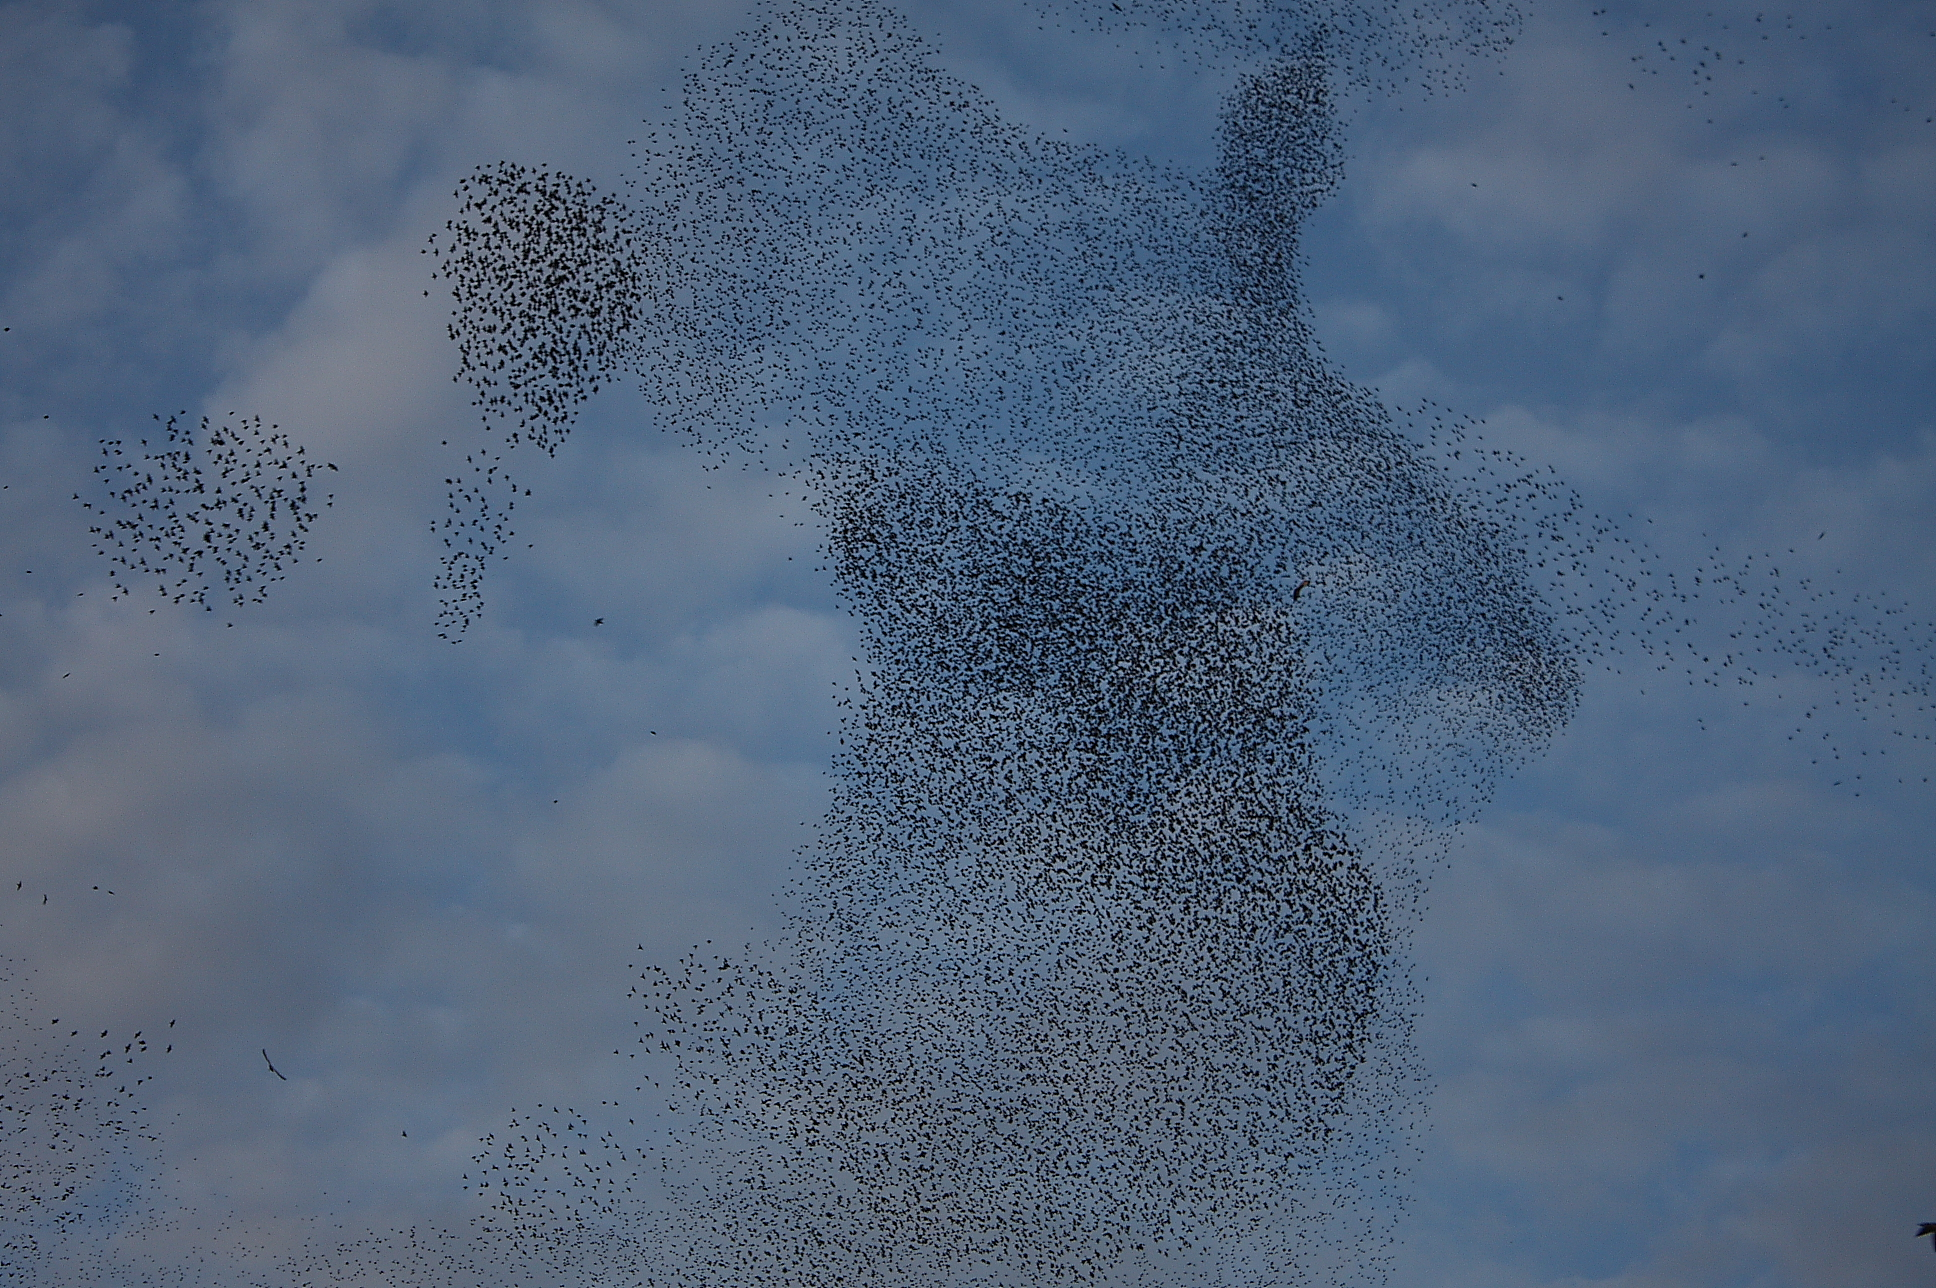
\includegraphics[width=0.95\textwidth]{danza_degli_storni.jpg}
  \begin{center}
    {\large ``La danza degli storni''}\par
    Foto di \_Peck\_\par
    \url{http://www.flickr.com/photos/_pek_/4113244536/}\par
    Licenza: Creative Commons Attribution 2.0\par
  \end{center}
\newpage


\section{Generalità sulle trasformazioni geometriche piane}\label{sect:generalita_trasformazioni}

\subsection{Introduzione e definizioni}

\begin{quote}
<<C'è una cosa straordinaria da vedere a Roma in questa fine d'autunno ed è il cielo gremito d'uccelli. Il terrazzo del signor Palomar è un buon punto d'osservazione [\ldots{}] Nell'aria viola del tramonto egli guarda affiorare da una parte del cielo un pulviscolo minutissimo, una nuvola d'ali che volano [\ldots{}] Quando si pensa agli uccelli migratori ci si immagina di solito una formazione di volo molto ordinata e compatta [\ldots{}] Quest'immagine non vale per gli storni, o almeno per questi storni autunnali nel cielo di Roma [\ldots{}]>>

\hfill{}Da \emph{Palomar} di Italo Calvino
\end{quote}

Il volo degli storni disegna nel cielo figure in continua trasformazione, come si può vedere dalle foto riportate nelle figure~\ref{fig:storni1} e~\ref{fig:storni2}.

\begin{figure*}[!htb]
\begin{center}
	\noindent\begin{minipage}{0.485\textwidth}
		\centering
		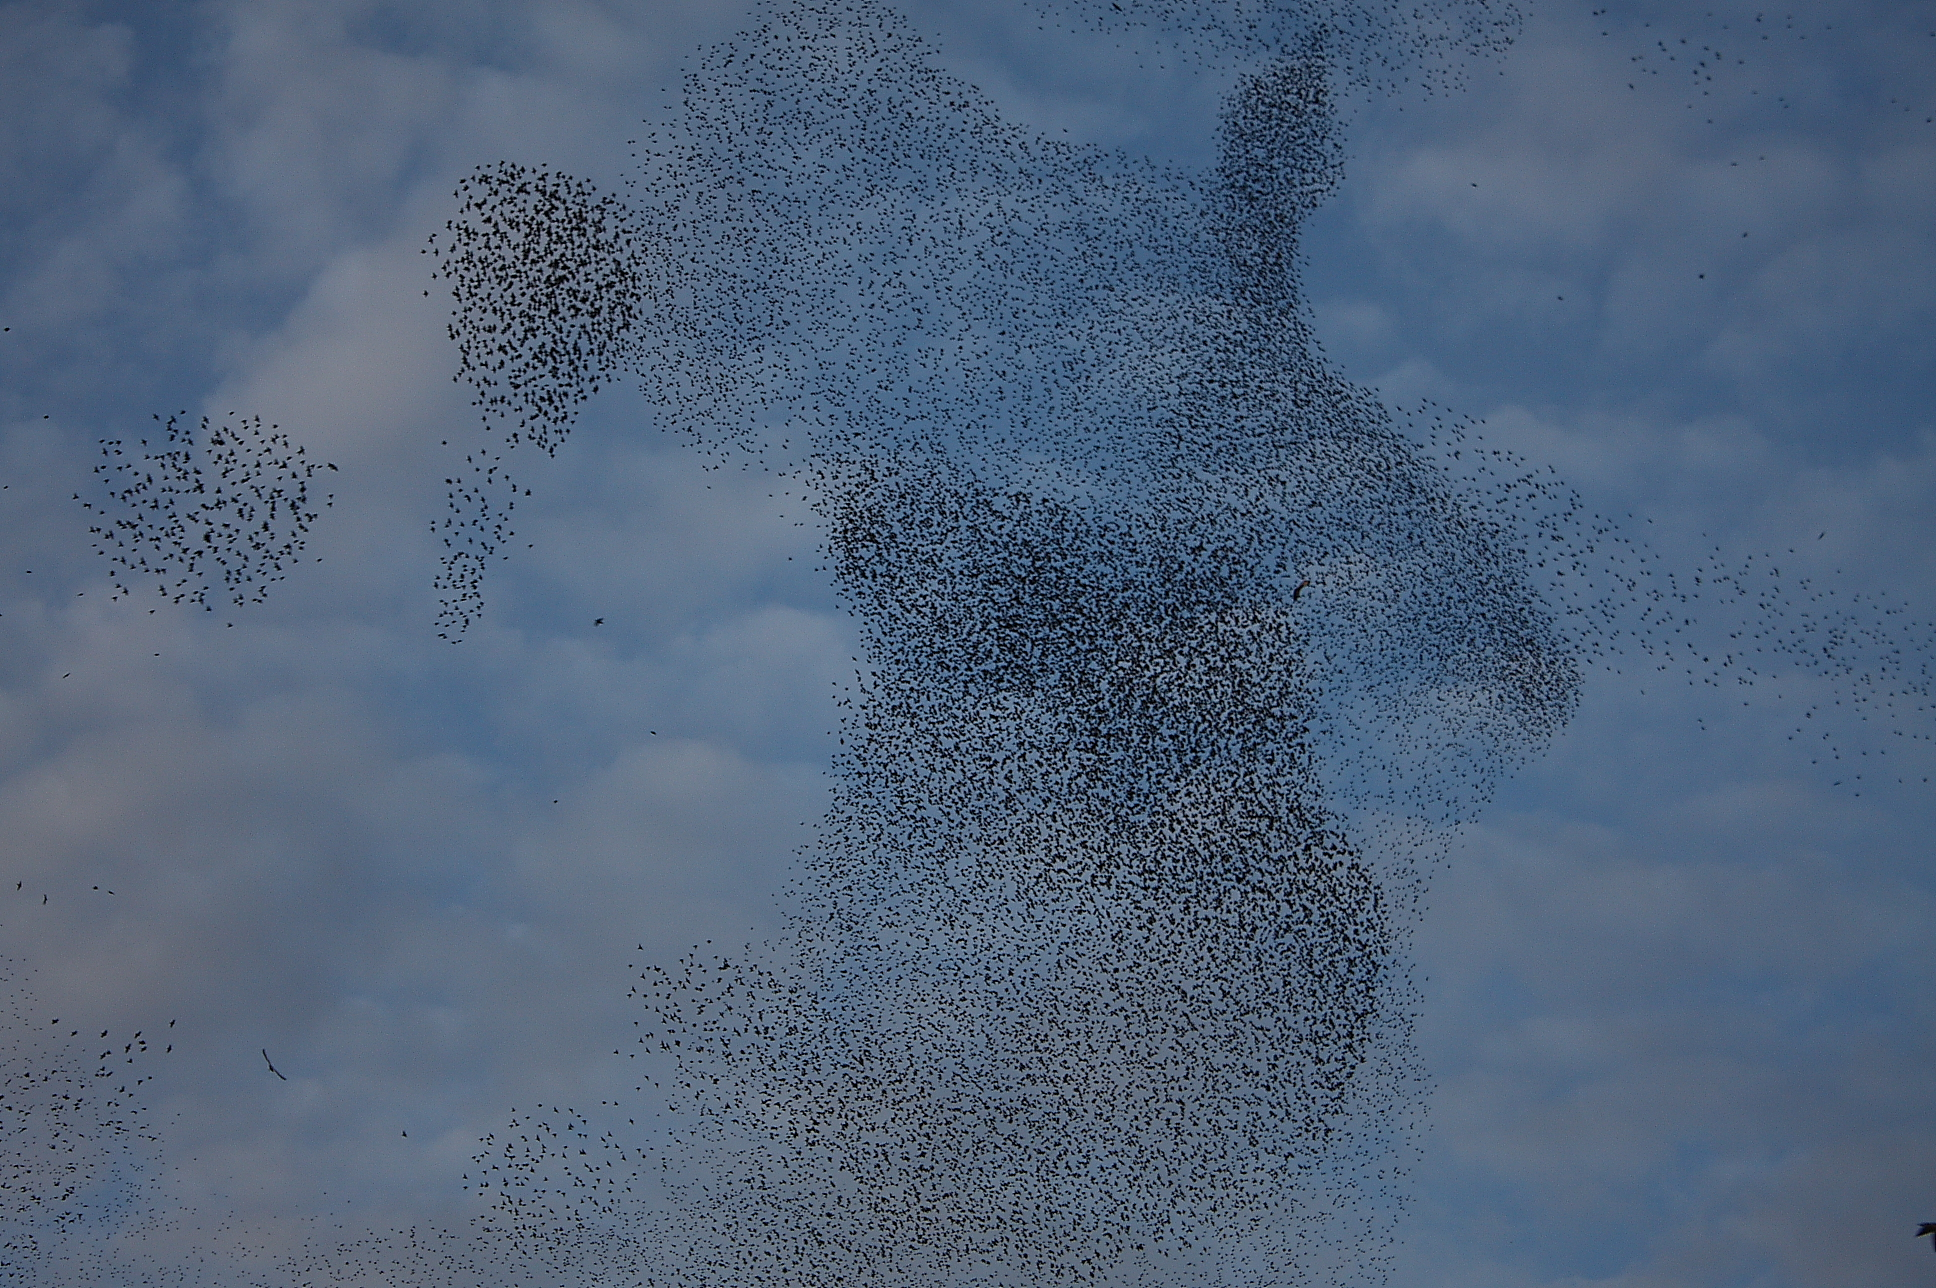
\includegraphics[width=\textwidth]{danza_degli_storni.jpg}
		\caption{\emph{La danza degli storni}
			\protect\footnotemark}\label{fig:storni1}
	\end{minipage}
	\hspace{2mm}	
	\noindent\begin{minipage}{0.47\textwidth}
		\centering
		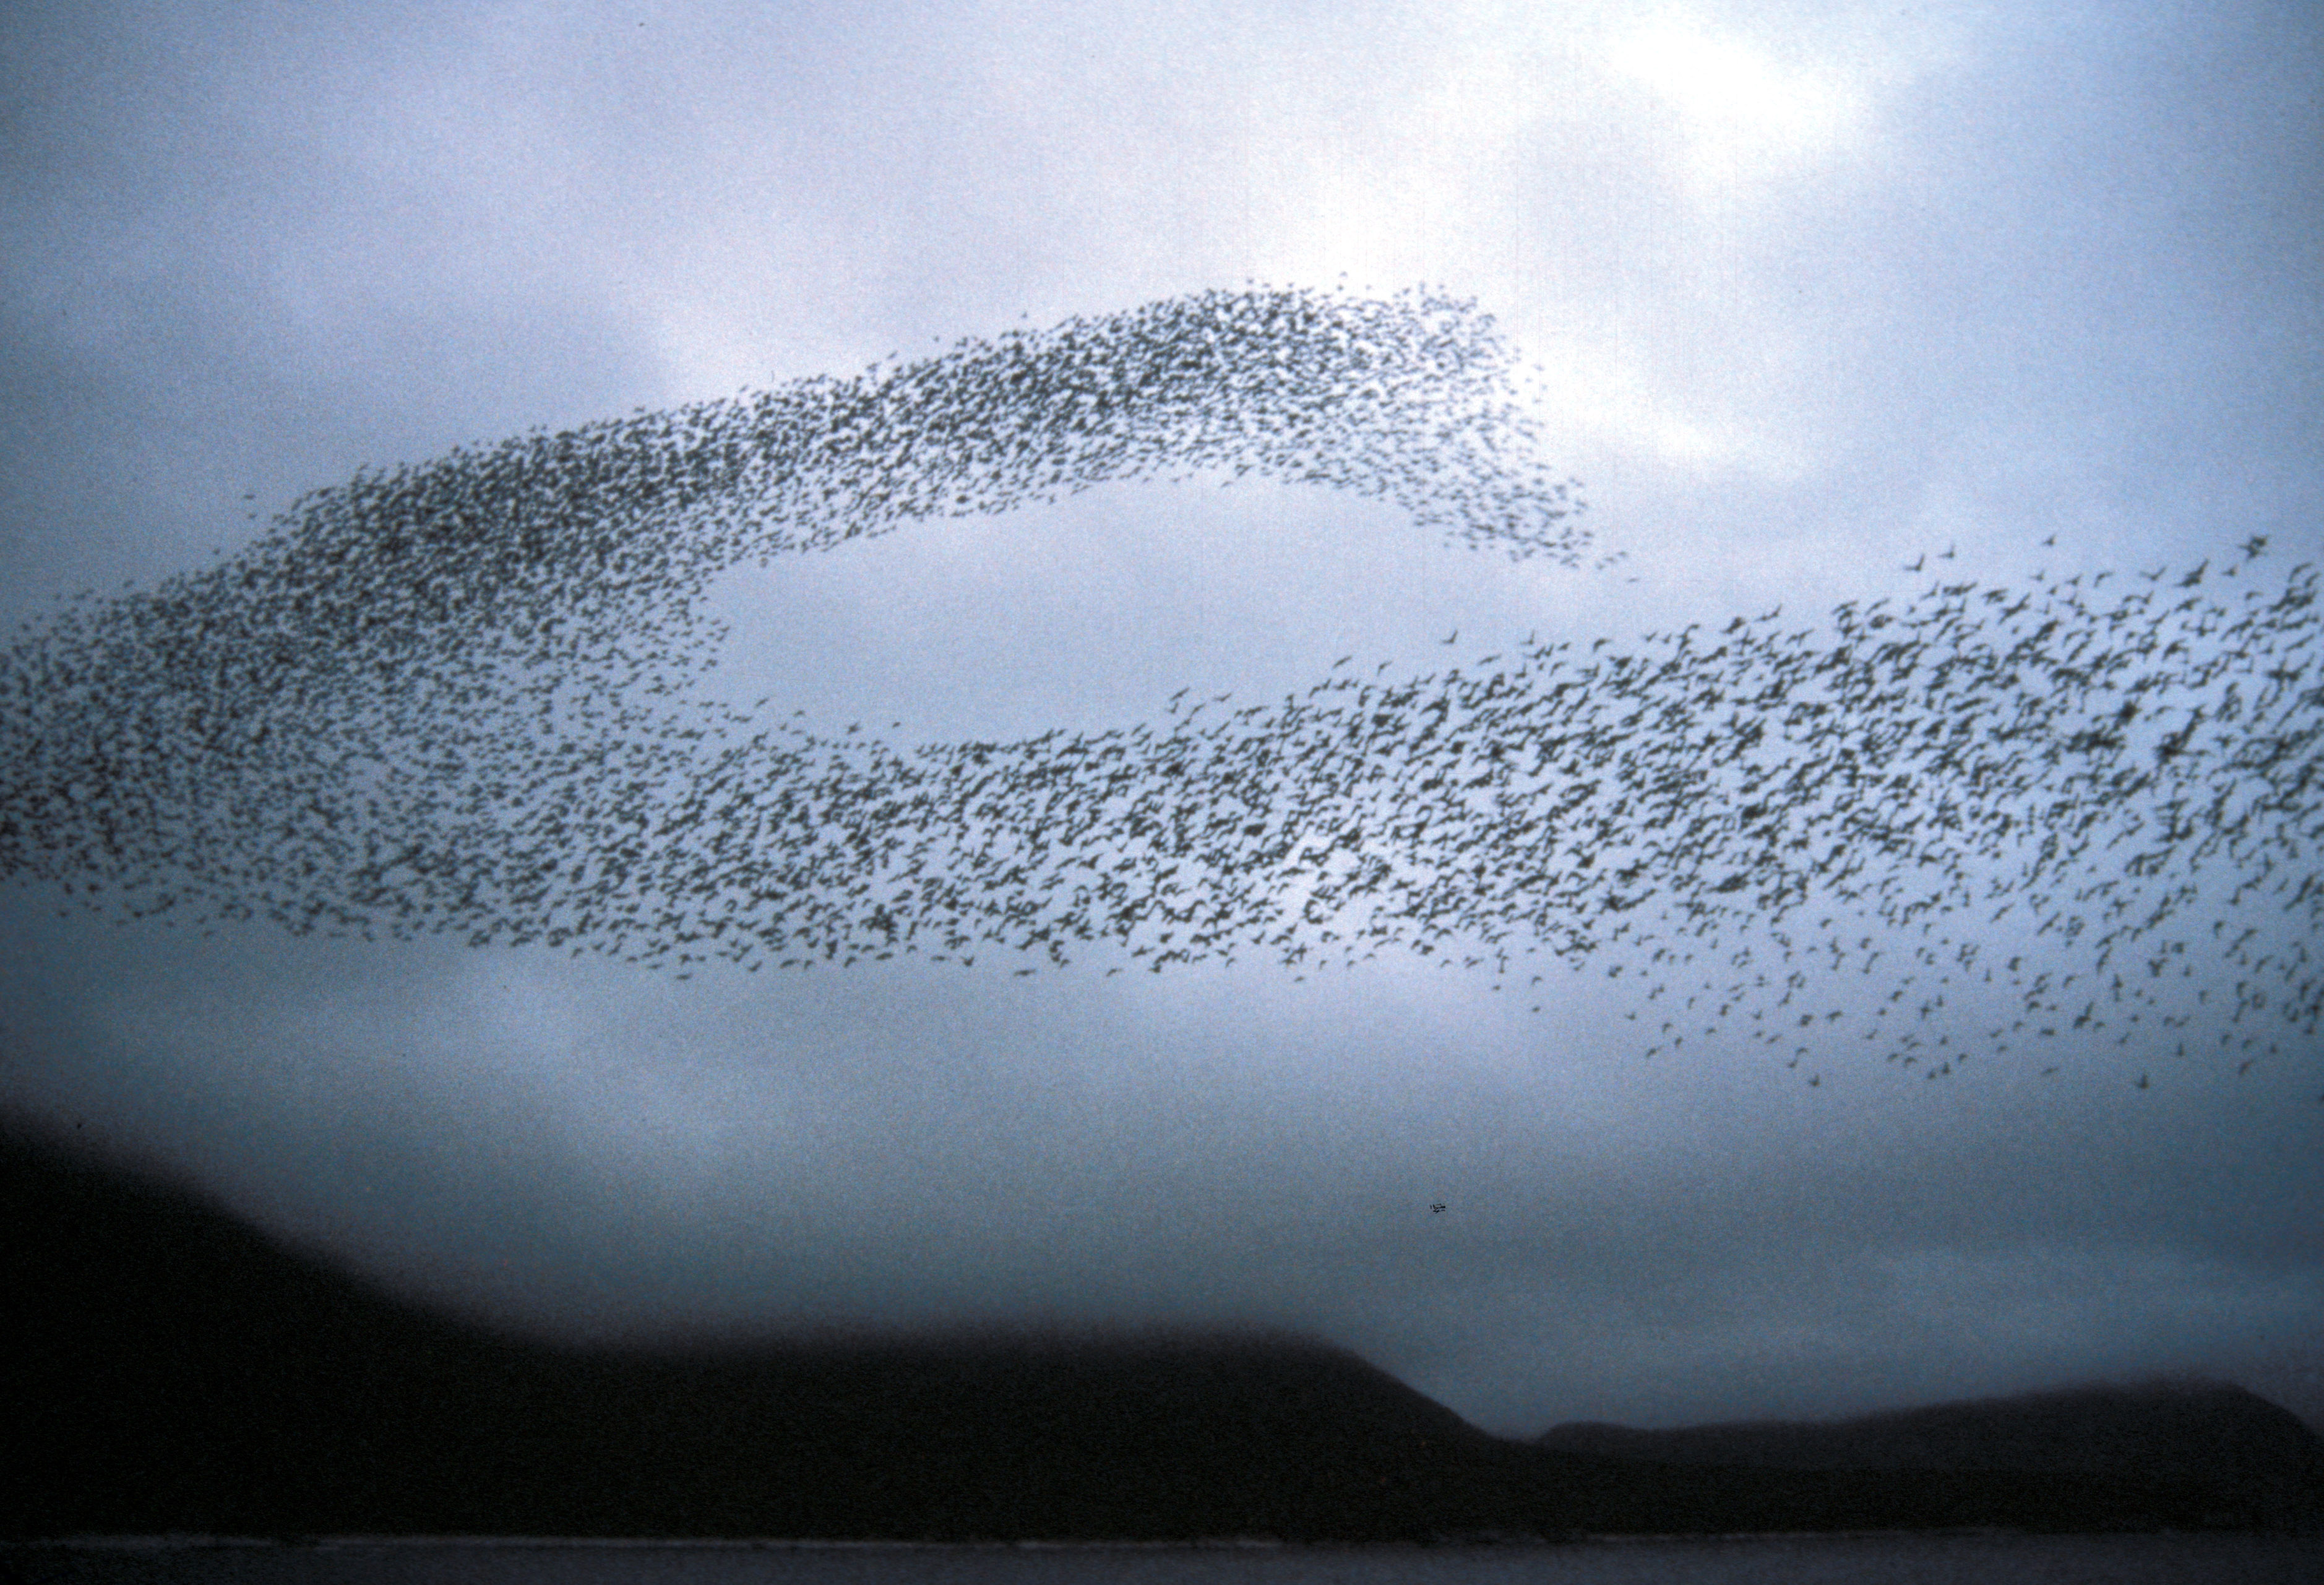
\includegraphics[width=\textwidth]{Auklet_flock_Shumagins_1986.jpg}
		\caption{\emph{Auklet flock, Shumagins 1986}\protect\footnotemark
			}\label{fig:storni2}
	\end{minipage}
\end{center}
\end{figure*}

\footnotetext[1]{foto di \_Peck\_, \url{http://www.flickr.com/photos/_pek_/4113244536/}.}
\footnotetext[2]{foto di D. Dibenski, \url{http://commons.wikimedia.org/wiki/File:Auklet_flock_Shumagins_1986.jpg}.}

%\begin{figure}[!htb]
%	\begin{minipage}{0.4\textwidth}
%		\centering
%		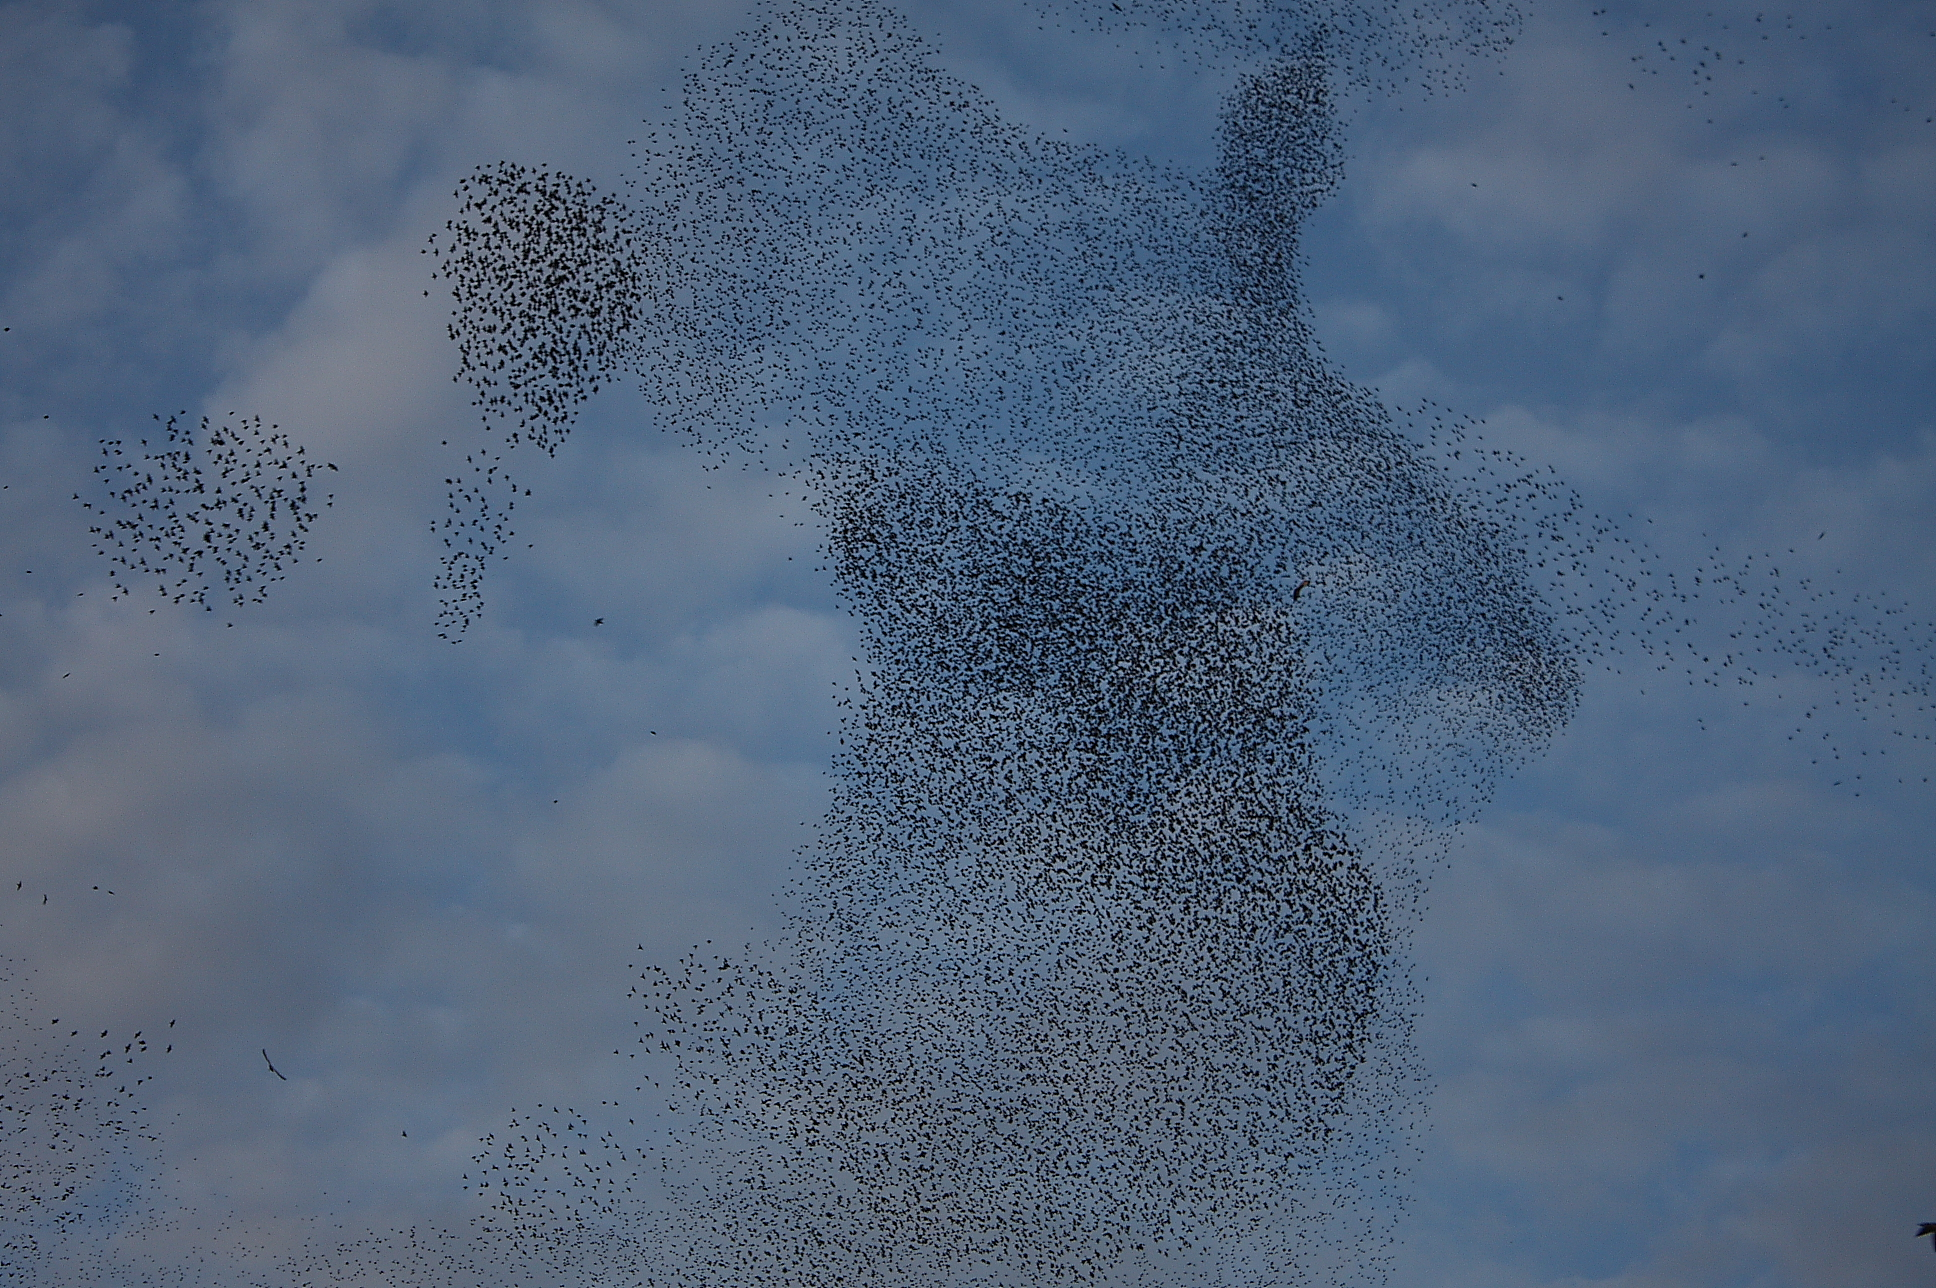
\includegraphics[width=0.4\textwidth]{danza_degli_storni.jpg}
%		\caption{\emph{La danza degli storni}, foto di \_Peck\_\\\url{http://www.flickr.com/photos/_pek_/4113244536/}}\label{fig:storni1}
%	\end{minipage}
%	\ \hspace{1cm} \
%	\begin{minipage}{0.4\textwidth}
%		\centering
%		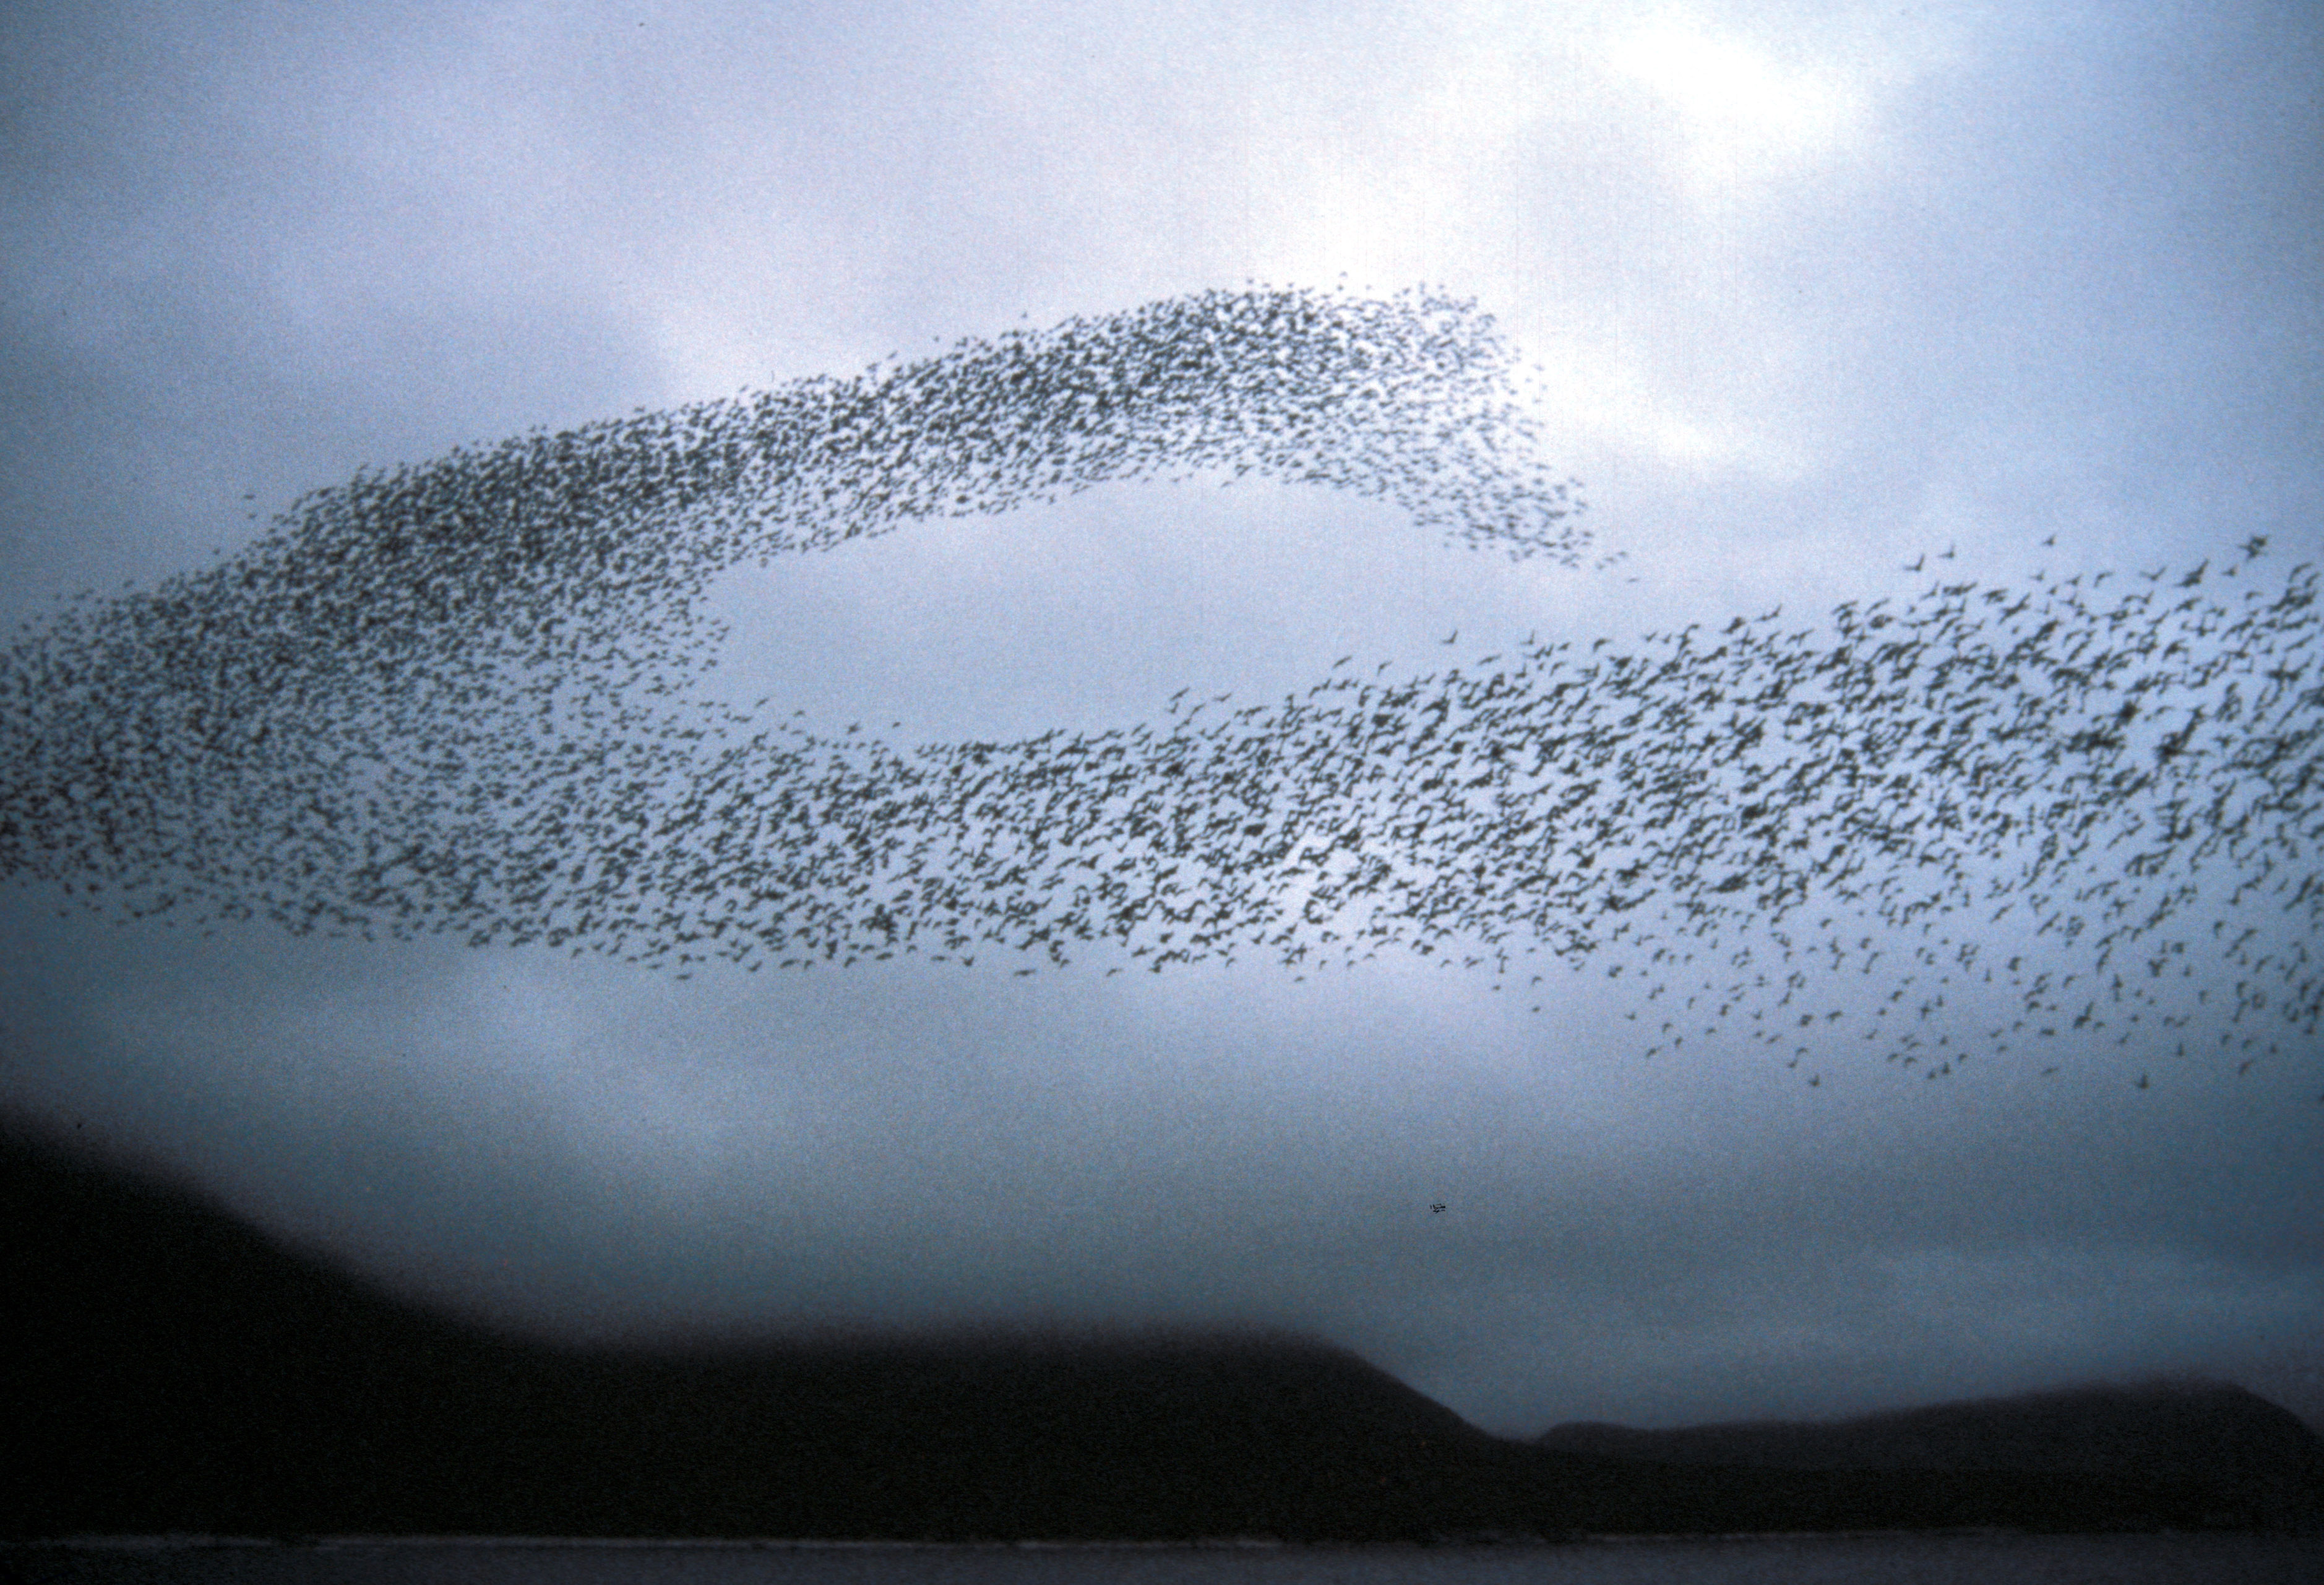
\includegraphics[width=0.4\textwidth]{Auklet_flock_Shumagins_1986.jpg}
%		\caption{\emph{Auklet flock, Shumagins 1986}, foto di D. Dibenski\\\url{http://commons.wikimedia.org/wiki/File:Auklet_flock_Shumagins_1986.jpg}}\label{fig:storni2}
%	\end{minipage}
%\end{figure}

Il concetto di trasformazione assume significati diversi a secondo dell'ambito in cui è definito: ad esempio in zoologia la trasformazione di un animale dallo stadio di larva allo stadio di adulto è più propriamente chiamata ``metamorfosi''. Ciò provoca un cambiamento totale del corpo del giovane e l'adulto quasi sempre avrà una forma molto differente da quella della larva (figura~\ref{fig:tadpole}).

Il gioco del tangram (vedi pagina~\pageref{tangram}) si basa sulla capacità di passare da una figura ad un'altra senza che nessun pezzo del quadrato base venga tagliato o modificato nelle sue dimensioni: le figure che si ottengono (come quella riportata nella figura~\ref{fig:tangramman}) hanno forme diverse, ma sono costituite dagli stessi pezzi. Possiamo dire che le une vengono trasformate nelle altre grazie alla nostra fantasia.

\begin{figure}[!htb]
\begin{center}
 \noindent\begin{minipage}{0.6\textwidth}
   \centering
   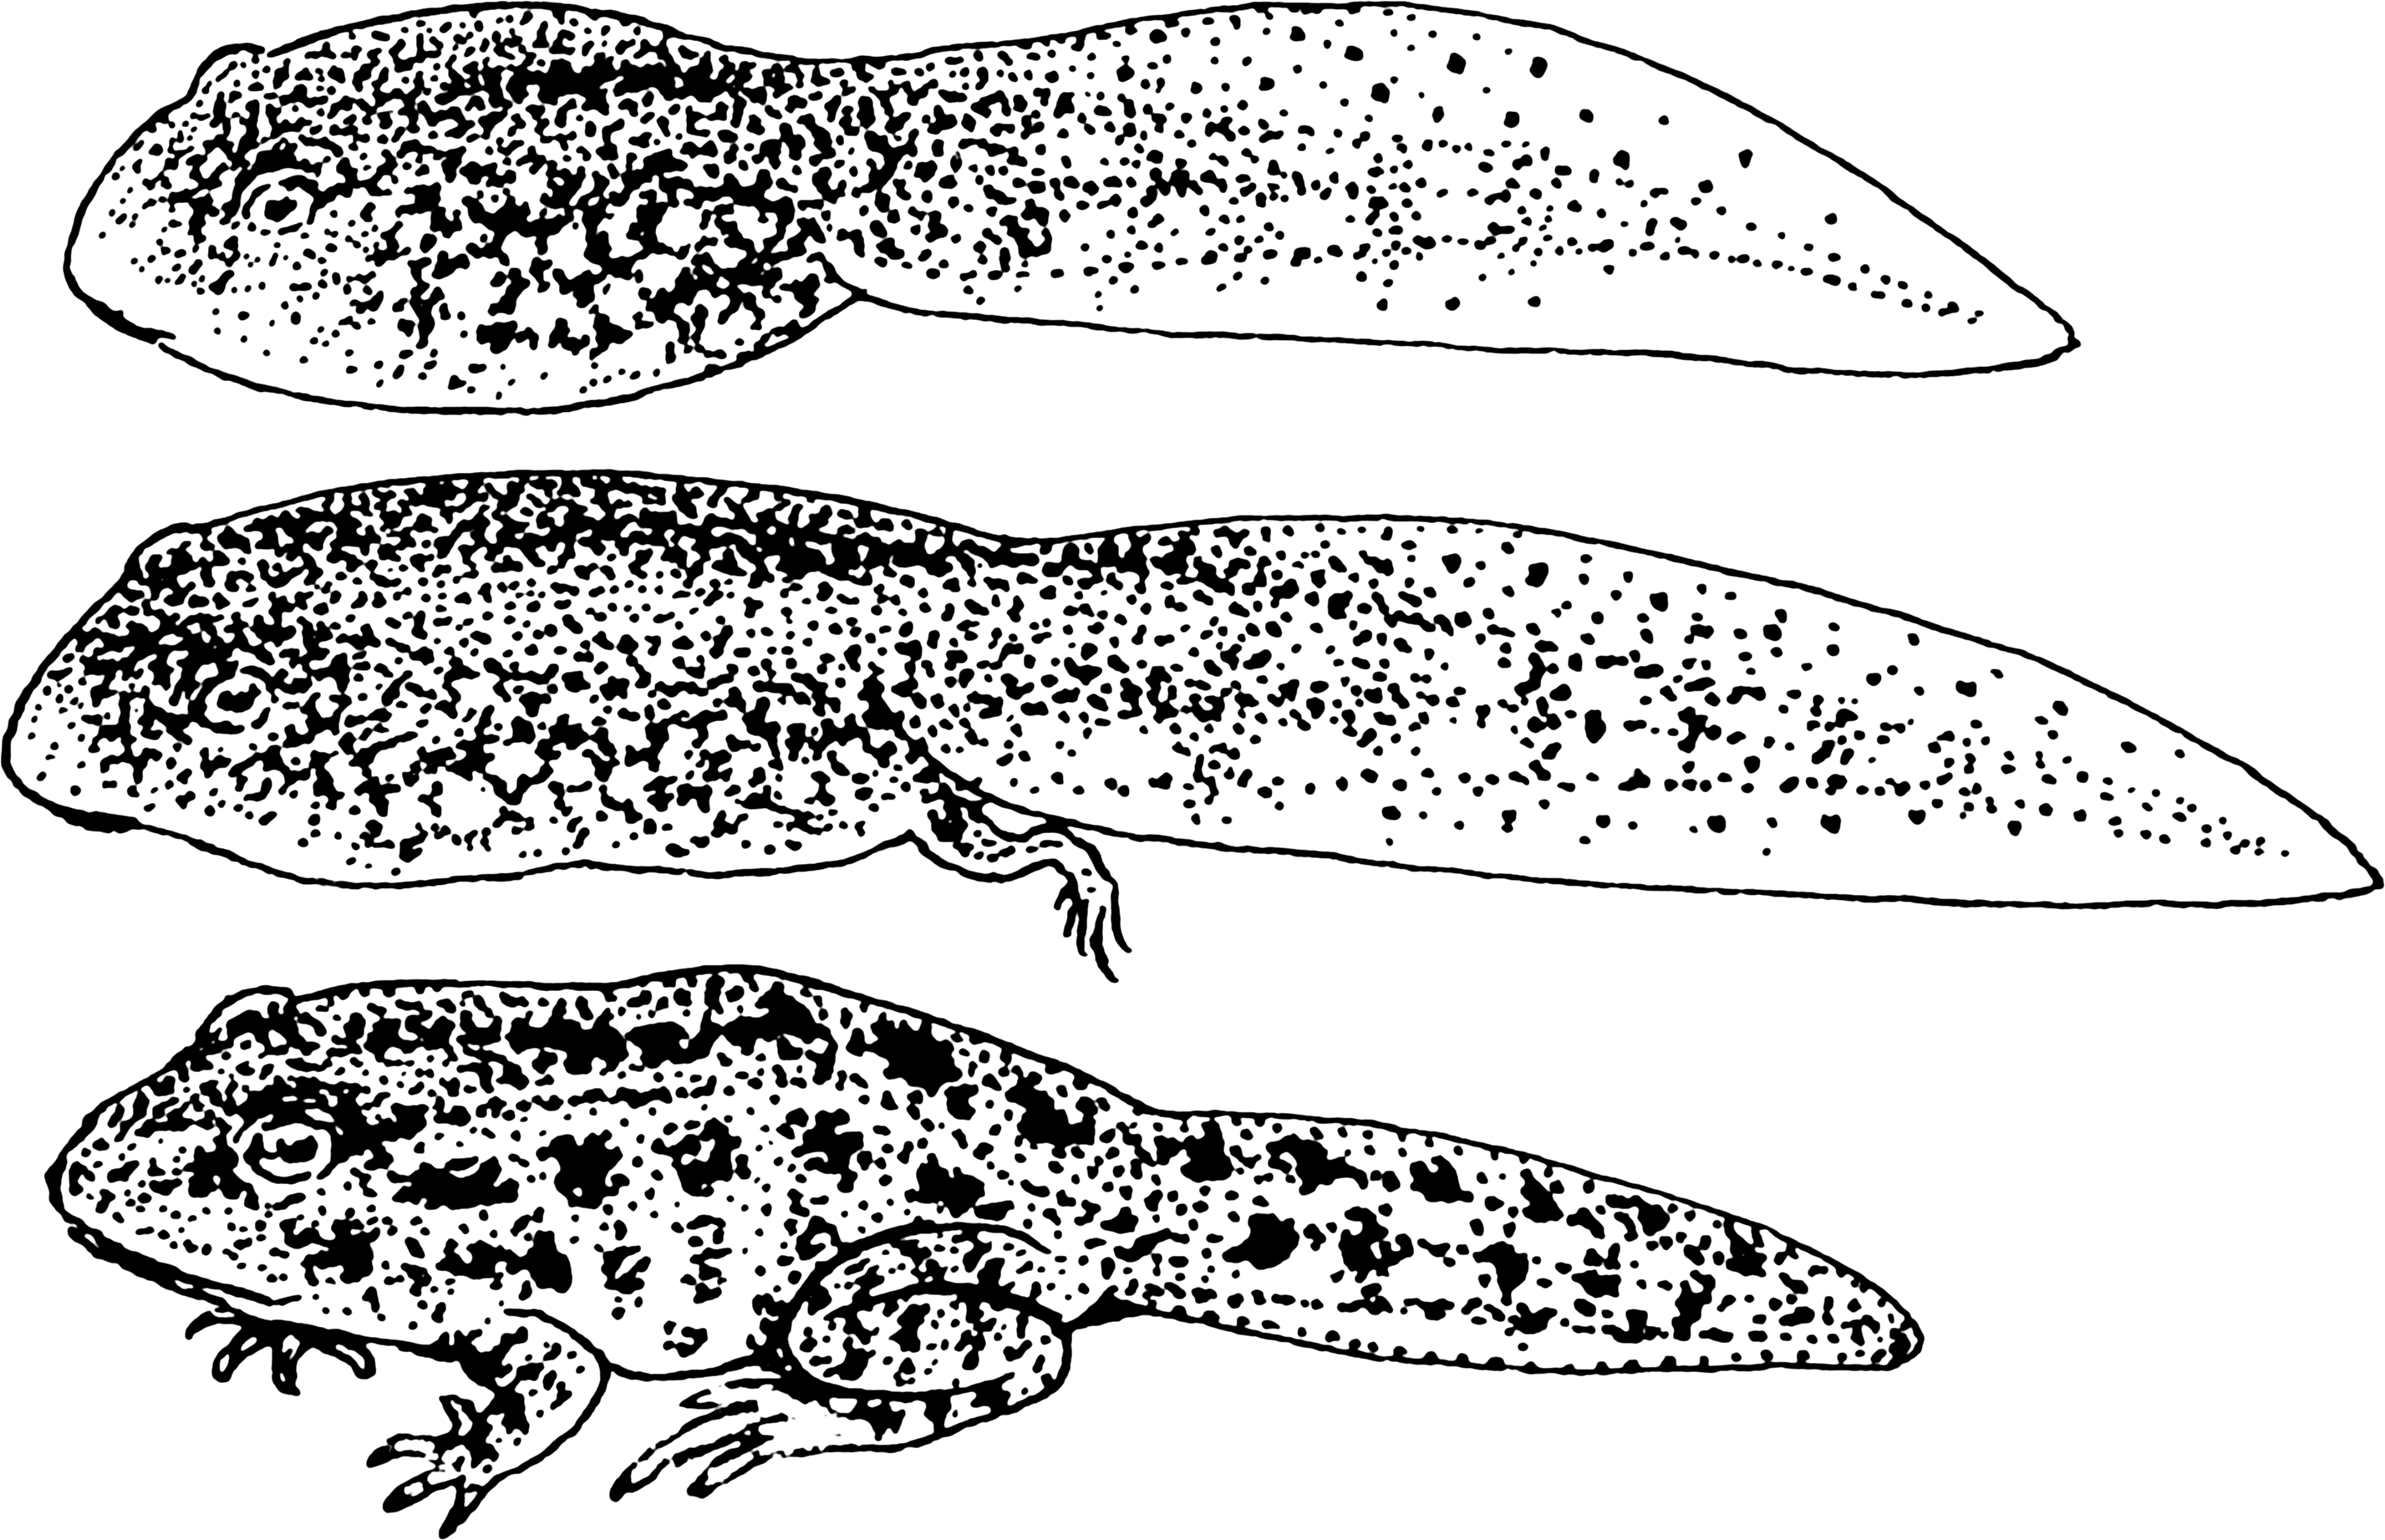
\includegraphics[width=\textwidth]{Tadpole_(PSF).png}
   \caption{\emph{Line art representation of w:Tadpole}\protect\footnotemark}\label{fig:tadpole}
 \end{minipage}
\hspace{7mm}
 \noindent\begin{minipage}{0.26\textwidth}
  \centering
   
\includegraphics[width=\textwidth]{2000px-Tangram-man.png}
   \caption{\emph{Tangram-man}\protect\footnotemark}\label{fig:tangramman}
 \end{minipage}
\end{center}
\end{figure}

%\begin{figure}[!htb]
%	\begin{minipage}{0.4\textwidth}
%		\centering
%		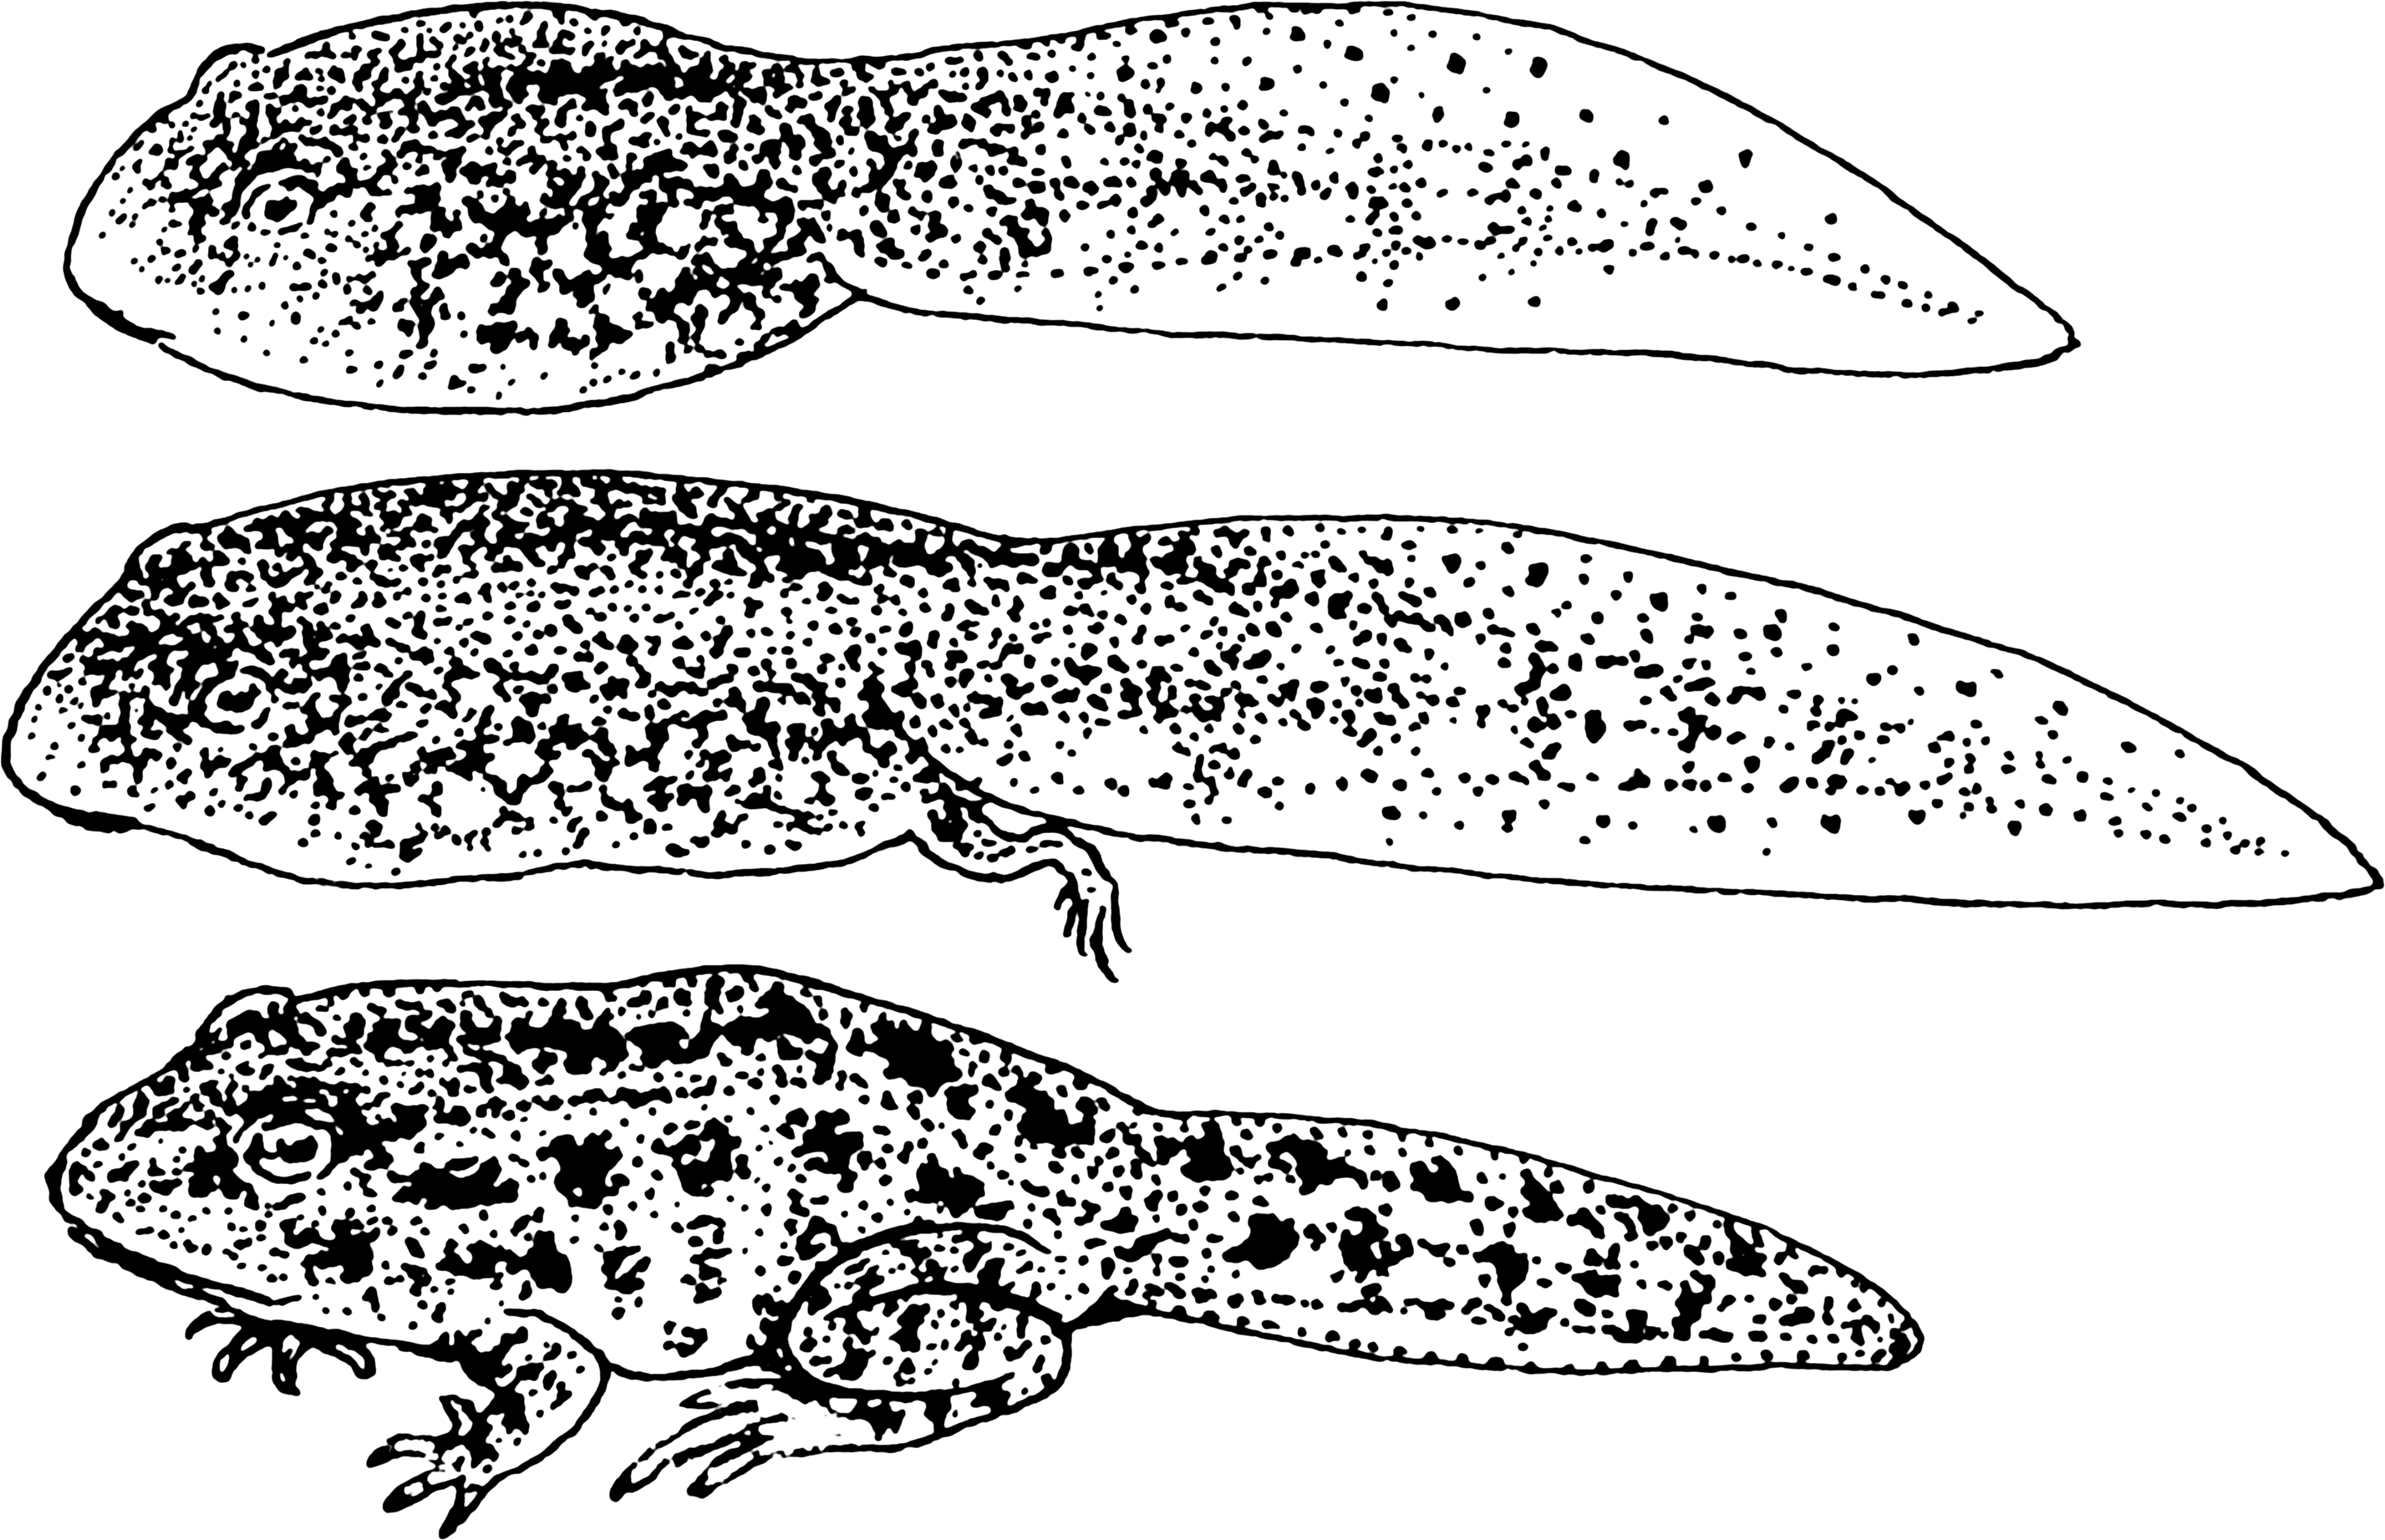
\includegraphics[width=0.4\textwidth]{Tadpole_(PSF).png}
%		\caption{\emph{Line art representation of w:Tadpole}, immagine di Pearson Scott Foresman\\\url{http://commons.wikimedia.org/wiki/File:Tadpole_\%28PSF\%29.png}}\label{fig:tadpole}
%	\end{minipage}
%	\ \hspace{1cm} \
%	\begin{minipage}{0.4\textwidth}
%		\centering
%		\includegraphics[width=0.4\textwidth]{Tangram.png}
%		\caption{\emph{Tangram-man}, immagine di Actam\\
%			\url{http://commons.wikimedia.org/wiki/File:Tangram-man.svg}}\label{fig:tangramman}
%	\end{minipage}
%\end{figure}

In geometria le trasformazioni sono particolari corrispondenze aventi come dominio e codominio il piano considerato come insieme di punti. Più precisamente si enuncia la seguente

\begin{definizione}
Si definisce \emph{trasformazione geometrica piana} una corrispondenza biunivoca tra punti del piano.
\end{definizione}

Attraverso una legge ben definita, una trasformazione geometrica piana associa ad un punto $P$ del piano uno e un solo punto $P'$ dello stesso piano e, viceversa, il punto $P'$ risulta essere il corrispondente di un solo punto $P$ del piano. Diciamo che $P'$ è l'\emph{immagine di $P$} nella trasformazione considerata.

\footnotetext[3]{immagine di Pearson Scott Foresman, \url{http://commons.wikimedia.org/wiki/File:Tadpole\_\%28PSF\%29.png}.}
\footnotetext[4]{immagine di Actam, \url{http://commons.wikimedia.org/wiki/File:Tangram-man.svg}.}

Indicata con $\Phi$ la legge della corrispondenza che individua la trasformazione, per esprimere il legame tra $P$ e $P'$ scriveremo

\noindent{\begin{center}\fbox{$\Phi:P\rightarrow P'$}\qquad o anche\qquad \fbox{$P\overset{\Phi}{\rightarrow}P'$}\end{center}}

\noindent e leggeremo: ``$\Phi$ fa corrispondere al punto $P$ il punto $P'$'', oppure

\noindent{\begin{center}\fbox{$\Phi(P)=P'$}\end{center}}

\noindent e leggeremo: ``$\Phi$ di $P$ è uguale a $P'$'', scrittura che definisce la trasformazione geometrica come funzione del punto preso in considerazione.

La trasformazione $\Phi$ fa corrispondere ad una figura $\Omega$ del piano la figura $\Omega'$ costituita dalle immagini dei punti della figura iniziale. $\Omega'$ è detta dunque \emph{immagine di $\Omega$ secondo $\Phi$}, in formule $\Phi: \Omega \rightarrow \Omega'$ o anche $\Omega\overset{\Phi}{\rightarrow}\Omega'$ o ancora $\Phi(\Omega)=\Omega'$.

Le trasformazioni geometriche che studieremo sono tali da far corrispondere ad una retta $r$ la retta $r'$ individuata dai punti $A'$ e $B'$ immagini di due punti $A$ e $B$ scelti arbitrariamente su $r$. Tali trasformazioni sono chiamate \emph{collineazioni}.

\begin{definizione}
Un punto $P$ che coincide con la propria immagine $P'$ è detto \emph{punto unito} o \emph{fisso} nella trasformazione $\Phi$ considerata.
\end{definizione}

Nel caso in cui tutti i punti del piano coincidono con la propria immagine, la trasformazione è detta \emph{identità}.

Per descrivere una trasformazione geometrica è quindi necessario definire come si costruisce l'immagine di un qualunque punto del piano.

\begin{exrig}
\begin{esempio}\label{es:8.1}
Consideriamo nel piano la seguente corrispondenza: fissato un punto $K$ la corrispondenza $S_K$ associa ad ogni punto $P$ del piano il punto $P'$ dello stesso piano tale che $K$ risulti il punto medio del segmento $PP'$. $S_K$ è una trasformazione geometrica?\vspace{7pt}

La definizione è costruttiva:
\[P\overset{S_K}{\rightarrow}P' \wedge PK\cong KP'\text{,} \quad  A\overset{S_K}{\rightarrow}A' \wedge AK\cong KA'\]

Per dimostrare che la corrispondenza è una trasformazione geometrica dobbiamo verificare che si tratta di una corrispondenza biunivoca tra punti del piano: ogni punto ha un corrispondente secondo $S_K$ e, viceversa, ogni punto è immagine di un solo punto del piano stesso. Il punto $K$ è corrispondente di se stesso dunque è un punto unito della trasformazione, anzi è l'unico punto unito (figura~\ref{fig:es8.1a}).

\begin{figure}[!htb]
\begin{center}
 \noindent\begin{minipage}{0.4\textwidth}
    \centering% Copyright (c) 2015 Daniele Masini - d.masini.it@gmail.com

\begin{tikzpicture}[scale=0.9,font=\small]
\usetikzlibrary{calc}

\begin{scope}
\coordinate (k) at (0,0);
\coordinate (a) at (-0.1,-1);
\coordinate (p) at (1.5,0.7);

\draw[dotted] (p) let \p1 = (p) in -- ({-\x1},{-\y1}) coordinate (p1);
\draw[dotted] (a) let \p1 = (a) in -- ({-\x1},{-\y1}) coordinate (a1);

\draw[blue, fill] (k) circle (1pt) node[black, shift={(-0.2,0.2)}] {$K$};
\draw[fill] (a) circle (1pt) node[shift={(-0.15,0.2)}] {$A$};
\draw[fill] (p) circle (1pt) node[shift={(-0.1,0.2)}] {$P$};
\draw[fill] (a1) circle (1pt) node[shift={(-0.15,0.2)}] {$A'$};
\draw[fill] (p1) circle (1pt) node[shift={(-0.1,0.2)}] {$P'$};

\end{scope}


\end{tikzpicture}

	\caption{Esempio~\ref{es:8.1}}\label{fig:es8.1a}
 \end{minipage}
 %\hspace{0.05\textwidth}
 \noindent\begin{minipage}{0.4\textwidth}
    \centering% (c) 2014 Daniele Masini - d.masini.it@gmail.com
\begin{tikzpicture}[scale=0.65,font=\small]
\usetikzlibrary{calc}

\clip (-3.5,-2.5) rectangle (3.5,2.5);
\begin{scope}
\coordinate (k) at (0,0);
\coordinate (a) at (-1.5,-2);
\coordinate (b) at (-3,-2);
\coordinate (c) at (-3,-0.5);
\coordinate (d) at (-1.5,-0.5);

\path (a) let \p1 = (a) in -- ({-\x1},{-\y1}) coordinate (a1);
\path (b) let \p1 = (b) in -- ({-\x1},{-\y1}) coordinate (b1);
\path (c) let \p1 = (c) in -- ({-\x1},{-\y1}) coordinate (c1);
\path (d) let \p1 = (d) in -- ({-\x1},{-\y1}) coordinate (d1);

\draw[thick, fill=red!10] (a) -- (b) -- (c) -- (d) -- cycle;
\draw[thick, fill=blue!10] (a1) -- (b1) -- (c1) -- (d1) -- cycle;

\draw[dotted] (a) -- (a1);
\draw[dotted] (b) -- (b1);
\draw[dotted] (c) -- (c1);
\draw[dotted] (d) -- (d1);

\draw[blue, fill] (k) circle (1pt) node[black, shift={(-0.2,0.2)}] {$K$};
\draw[fill] (a) circle (1pt) node[shift={(0.2,-0.2)}] {$A$};
\draw[fill] (b) circle (1pt) node[shift={(-0.2,-0.2)}] {$B$};
\draw[fill] (c) circle (1pt) node[shift={(-0.2,0.2)}] {$C$};
\draw[fill] (d) circle (1pt) node[shift={(0.2,0.2)}] {$D$};
\draw[fill] (a1) circle (1pt) node[shift={(-0.2,0.2)}] {$A'$};
\draw[fill] (b1) circle (1pt) node[shift={(0.2,0.2)}] {$B'$};
\draw[fill] (c1) circle (1pt) node[shift={(0.2,-0.2)}] {$C'$};
\draw[fill] (d1) circle (1pt) node[shift={(-0.2,-0.2)}] {$D'$};

\end{scope}


\end{tikzpicture}

    \caption{Esempio~\ref{es:8.1}}\label{fig:es8.1b}
 \end{minipage}
\end{center}
\end{figure}

Nella figura~\ref{fig:es8.1b} è rappresentato come opera la trasformazione $S_K$ se applicata ad un quadrato.
\[AK\cong KA'\text{, }BK\cong KB'\text{, }CK\cong KC'\text{, }DK\cong KD'\]

$ABCD\overset{S_K}{\rightarrow}A'B'C'D'$ e i due quadrati hanno le stesse dimensioni.
\end{esempio}

\begin{esempio}\label{es:8.2}
Definiamo la seguente trasformazione geometrica $\Phi$ sul generico punto $P$: dato un punto $O$, tracciamo la semiretta uscente da $O$ e passante per $P$; il punto $P'$, trasformato di $P$ secondo $\Phi$, è il punto della semiretta tale che $OP'=2OP$.\vspace{7pt}

\begin{figure}[!htb]
    \centering% Copyright (c) 2015 Daniele Masini - d.masini.it@gmail.com

\begin{tikzpicture}[scale=0.7,font=\small]
\usetikzlibrary{calc}

\pgfmathsetmacro{\const}{2.5}

\begin{scope}
\coordinate (o) at (0,0);
\coordinate (a) at (-3,-0.5);
\coordinate (b) at (-1.5,-0.5);
\coordinate (c) at (-1.5,-2);
\coordinate (d) at (-3,-2);

\path (a) let \p1 = (a) in -- ({\x1*\const},{\y1*\const}) coordinate (a1);
\path (b) let \p1 = (b) in -- ({\x1*\const},{\y1*\const}) coordinate (b1);
\path (c) let \p1 = (c) in -- ({\x1*\const},{\y1*\const}) coordinate (c1);
\path (d) let \p1 = (d) in -- ({\x1*\const},{\y1*\const}) coordinate (d1);

\draw[thick, fill=red!10] (a) -- (b) -- (c) -- (d) -- cycle;
\draw[thick, fill=blue!10] (a1) -- (b1) -- (c1) -- (d1) -- cycle;

\draw[dotted] (o) -- (a1);
\draw[dotted] (o) -- (b1);
\draw[dotted] (o) -- (c1);
\draw[dotted] (o) -- (d1);

\draw[blue, fill] (o) circle (1pt) node[black, shift={(0.2,0.2)}] {$O$};
\draw[fill] (a) circle (1pt) node[shift={(-0.2,0.2)}] {$A$};
\draw[fill] (b) circle (1pt) node[shift={(0.2,0.2)}] {$B$};
\draw[fill] (c) circle (1pt) node[shift={(0.2,-0.2)}] {$C$};
\draw[fill] (d) circle (1pt) node[shift={(-0.2,-0.2)}] {$D$};
\draw[fill] (a1) circle (1pt) node[shift={(-0.2,0.2)}] {$A'$};
\draw[fill] (b1) circle (1pt) node[shift={(0.2,0.2)}] {$B'$};
\draw[fill] (c1) circle (1pt) node[shift={(0.2,-0.2)}] {$C'$};
\draw[fill] (d1) circle (1pt) node[shift={(-0.2,-0.2)}] {$D'$};

\end{scope}


\end{tikzpicture}

	\caption{Esempio~\ref{es:8.2}}\label{fig:es8.2}
\end{figure}

Applicando questa trasformazione al quadrato $ABCD$ (figura~\ref{fig:es8.2}) quest'ultimo si trasforma in un altro quadrato ma le due figure non hanno le stesse dimensioni.
\end{esempio}
\end{exrig}

Se il piano è dotato di un riferimento cartesiano ortogonale, la legge della trasformazione geometrica piana lega le coordinate di un punto e quelle del suo corrispondente mediante equazioni o sistemi di equazioni.
 
\begin{definizione}
Chiamiamo \emph{equazione della trasformazione} l'insieme delle espressioni algebriche che indicano come si passa dalle coordinate di un generico punto $P$ a quelle della sua immagine $P'$.
\end{definizione}

\begin{exrig}
\begin{esempio}\label{es:8.3}
La corrispondenza $\Phi$ associa ad un punto $P$ del piano dotato di riferimento cartesiano ortogonale il punto $P'$ secondo la seguente legge:
$\Phi : P(x_P;y_P) \rightarrow P'(-2x_P;x_P-y_P)$. La corrispondenza assegnata è una trasformazione geometrica piana?\vspace{7pt}

Strategia risolutiva: 
scegliamo un punto del piano: $P(\ldots{};\ldots{})$ e determiniamo $P'(\ldots{};\ldots{})$;
scegliamo un punto $Q'(\ldots{};\ldots{})$ e determiniamo la controimmagine $Q(\ldots{};\ldots{})$.
posso affermare che la corrispondenza è biunivoca perché \ldots\ldots\ldots\ldots{} e quindi posso affermare che è una trasformazione geometrica.

\begin{figure}[!htb]
\begin{center}
 \noindent\begin{minipage}{0.49\textwidth}
    \centering% (c) 2014 Daniele Masini - d.masini.it@gmail.com
\begin{tikzpicture}[scale=1,font=\small, x=5.9mm, y=5.9mm, smooth]
\usetikzlibrary{calc}

\begin{scope}

\begin{scope}[dotted,orange]
\draw[step=5.9mm] (-5.5,-5.5) grid (5.7,5.7);
\end{scope}

\begin{scope}[->]
\draw (-5.5,0) -- (5.7,0) node [below] {$x$};
\draw (0,-5.5) -- (0,5.7) node [left] {$y$};
\end{scope}

\foreach \x in {-5, -4, -3, -2, -1, 1, 2, 3, 4, 5}
\draw (\x,1.5pt) -- (\x,-1.5pt) node[below] {$\x$};

\foreach \y in {-5, -4, -3, -2, -1, 1, 2, 3, 4, 5}
\draw (1.5pt,\y) -- (-1.5pt,\y) node[left] {$\y$};

\node[below left] at (0,0) {O};
%\filldraw[fill=white, draw=black] (0,0) circle (2pt);

\end{scope}


\end{tikzpicture}

	\caption{Esempio~\ref{es:8.3}}\label{fig:es8.3a}
 \end{minipage}
 \noindent\begin{minipage}{0.49\textwidth}
    \centering% Copyright (c) 2015 Daniele Masini - d.masini.it@gmail.com

\begin{tikzpicture}[scale=1,font=\small, x=6.2mm, y=6.2mm, smooth]
\usetikzlibrary{calc}

\begin{scope}

\coordinate (a) at (-1,1);
\coordinate (b) at (-1,3);
\coordinate (c) at (-3,3);
\coordinate (d) at (-3,1);

\coordinate (a1) at (2,-2);
\coordinate (b1) at (2,-4);
\coordinate (c1) at (6,-6);
\coordinate (d1) at (6,-4);

\begin{scope}[dotted,orange]
\draw[step=6.2mm] (-3.7,-6.7) grid (6.7,3.9);
\end{scope}

\begin{scope}[->]
\draw (-3.7,0) -- (6.7,0) node [below] {$x$};
\draw (0,-6.7) -- (0,3.9) node [left] {$y$};
\end{scope}

\foreach \x in {-3, -2, -1, 1, 2, 3, 4, 5, 6}
\draw (\x,1.5pt) -- (\x,-1.5pt) node[below] {$\x$};

\foreach \y in {-6, -5, -4, -3, -2, -1, 1, 2, 3}
\draw (1.5pt,\y) -- (-1.5pt,\y) node[left] {$\y$};

\node[below left] at (0,0) {O};
%\filldraw[fill=white, draw=black] (0,0) circle (2pt);

\draw[fill=red!10] (a) node[shift={(0.1,-0.25)}] {$A$} -- (b) node[shift={(0.1,0.25)}] {$B$} -- (c) node[shift={(-0.1,0.25)}] {$C$} -- (d) node[shift={(-0.1,-0.25)}] {$D$} -- cycle;
\draw[fill=blue!10] (a1) node[shift={(-0.1,0.3)}] {$A_1$} -- (b1) node[shift={(-0.1,-0.3)}] {$B_1$} -- (c1) node[shift={(0.1,-0.3)}] {$C_1$} -- (d1) node[shift={(0.1,0.3)}] {$D_1$} -- cycle;

\end{scope}


\end{tikzpicture}

    \caption{Esempio~\ref{es:8.3}}\label{fig:es8.3b}
 \end{minipage}
\end{center}
\end{figure}


Applichiamo la stessa trasformazione al quadrato di vertici $A(-1;1)$, $B(-1;3)$, $C(-3;3)$, $D(-3;1)$ (figura~\ref{fig:es8.3b}).

La trasformazione fa corrispondere al quadrato $ABCD$ il parallelogramma $A_1B_1C_1D_1$ di coordinate $A_1(2;-2)$, $B_1(2;-4)$, $C_1(6;-6)$ e $D_1(6;-4)$. Essa ha cambiato la natura della figura geometrica di partenza, ma ha mantenuto il parallelismo tra i lati: $AB\parallel CD \overset{S_K}{\rightarrow} A_1B_1\parallel C_1D_1$, dove $A_1B_1=\Phi(AB)$ e $C_1D_1=\Phi(CD)$.
\end{esempio}
\end{exrig}

Si noti il fatto che esistono trasformazioni geometriche che mantengono invariate forma e dimensioni delle figure a cui sono applicate, altre che mantengono inalterate la forma ma non dimensioni ed altre ancora che non mantengono inalterata neppure la forma.

\begin{definizione}
Si chiamano \emph{proprietà invarianti di una trasformazione} le caratteristiche che una figura e la sua corrispondente mantengono inalterate nella trasformazione.
\end{definizione}

Le principali caratteristiche che una trasformazione può lasciare inalterate sono: la lunghezza dei segmenti, l'ampiezza degli angoli, il rapporto tra segmenti, la misura della superficie, il parallelismo dei segmenti, l'orientamento dei punti del piano, la direzione delle rette, la forma, il numero di lati delle figure.
In questo capitolo tratteremo solo delle trasformazioni che mantengono invariate sia la forma che le dimensioni delle figure.

\begin{definizione}
Si chiama \emph{isometria} una trasformazione piana che associa a due punti distinti $A$ e $B$ del piano i punti $A'$ e $B'$ tali che $AB$ e $A'B'$ risultano congruenti.
\end{definizione}

Solo il primo esempio, tra i precedenti, rappresenta una isometria. Per dimostrare che è una isometria dobbiamo dimostrare che segmenti corrispondenti sono congruenti. Consideriamo il segmento $AP$ e il suo corrispondente $A'P'$; dimostriamo che $AP\cong A'P'$. Considero i triangoli $AKP$ e $A'KP'$, hanno \ldots\ldots\ldots{}
Lasciamo al lettore lo sviluppo della dimostrazione.

Riportiamo di seguito le proprietà di una isometria:
\begin{itemize*}
\item l'immagine di una retta è una retta, l'immagine di una semiretta è una semiretta, l'immagine di un segmento è un segmento ad esso congruente;
\item a rette parallele corrispondono rette parallele;
\item a rette incidenti corrispondono rette incidenti;
\item ad un angolo corrisponde un angolo ad esso congruente.
\end{itemize*}

\begin{definizione}
In una isometria $\Sigma$, una \emph{retta} è \emph{unita} se coincide con la sua immagine, cioè ogni punto della retta data ha come corrispondente un punto della stessa retta.
Nel caso in cui ogni punto di essa sia un punto unito, la retta è luogo di punti uniti e viene detta \emph{retta fissa}.
\end{definizione}

%Può succedere che ogni punto di una retta sia un punto unito: in tal caso la retta unita è luogo di punti uniti o \emph{retta fissa}.

\noindent\begin{minipage}{0.6\textwidth}\parindent15pt
\noindent $\left.\begin{array}{lll} A\in r \;\wedge\; B\in r\\ \Sigma : (A\rightarrow A') \;\wedge\; (B\rightarrow B')\\ A'\in r \;\wedge\; B'\in r \end{array}\right\} \;\Rightarrow\; r\equiv r'$
\end{minipage}\hfil
\begin{minipage}{0.4\textwidth}
	\centering% (c) 2014 Daniele Masini - d.masini.it@gmail.com
\begin{tikzpicture}[scale=1,font=\small]
\usetikzlibrary{calc}

\begin{scope}

\coordinate (r1) at (0,0);
\coordinate (r2) at (5,0);

\coordinate (a) at (1.5,0);
\coordinate (b) at (2.8,0);
\coordinate (a1) at (3.7,0);
\coordinate (b1) at (4.3,0);

\draw[thick] (r1) node[below right] {$r\equiv r'$} -- (r2);

\draw[fill] (a) circle (1pt) node[above] {$A$};
\draw[fill] (b) circle (1pt) node[above] {$B$};
\draw[fill] (a1) circle (1pt) node[above] {$A'$};
\draw[fill] (b1) circle (1pt) node[above] {$B'$};

\node at (2.5, -0.5) {retta unita};
\end{scope}


\end{tikzpicture}


\end{minipage}\vspace{8pt}

\noindent\begin{minipage}{0.6\textwidth}\parindent15pt
\noindent $\left.\begin{array}{lll} A\in r \;\wedge\; B\in r\\ \Sigma : (A\rightarrow A') \;\wedge\; (B\rightarrow B')\\ A'\equiv A \;\wedge\; B'\equiv B \end{array}\right\} \;\Rightarrow\; r\equiv r'$
\end{minipage}\hfil
\begin{minipage}{0.4\textwidth}
	\centering% (c) 2014 Daniele Masini - d.masini.it@gmail.com
\begin{tikzpicture}[scale=1,font=\small]
\usetikzlibrary{calc}

\begin{scope}

\coordinate (r1) at (0,0);
\coordinate (r2) at (5,0);

\coordinate (a) at (1.8,0);
\coordinate (b) at (4,0);

\draw[thick] (r1) node[below right] {$r\equiv r'$} -- (r2);

\draw[fill] (a) circle (1pt) node[above] {$A\equiv A'$};
\draw[fill] (b) circle (1pt) node[above] {$B\equiv B'$};

\node at (2.5, -0.5) {retta fissa};

\end{scope}


\end{tikzpicture}

\end{minipage}


\section{Le isometrie}\label{sect:isometrie}

Riprendiamo la definizione del paragrafo precedente: si chiama isometria una trasformazione piana che associa a due punti $A$ e $B$ del piano i punti $A'$ e $B'$ tali che $AB\cong A'B'$.

Richiamiamo anche le proprietà:
\begin{itemize*}
\item l'immagine di una retta è una retta, l'immagine di una semiretta è una semiretta, l'immagine di un segmento è un segmento ad esso congruente;
\item a rette parallele corrispondono rette parallele;
\item a rette incidenti corrispondono rette incidenti;
\item ad un angolo corrisponde un angolo ad esso congruente.
\end{itemize*}

Adesso ci proponiamo di studiare particolari isometrie.


\subsection{La simmetria centrale}

\begin{definizione}
Fissato nel piano un punto $K$, chiamiamo \emph{simmetria centrale di centro $K$} (indicata col simbolo $S_K$) la  corrispondenza che associa ad un punto $P$ del piano il punto $P'$ tale che $K$ risulti il punto medio del segmento $PP'$.
\end{definizione}

\noindent\begin{minipage}{0.65\textwidth}\parindent15pt
Per determinare l'immagine di un segmento è sufficiente determinare l'immagine dei suoi estremi. Nella figura a fianco è illustrato come agisce $S_K$ su una qualunque figura piana: l'immagine del triangolo $ABC$ è il triangolo $A'B'C'$ ottenuto determinando l'immagine di ciascuno dei suoi vertici.
\end{minipage}\hfil
\begin{minipage}{0.35\textwidth}
	\centering% (c) 2014 Daniele Masini - d.masini.it@gmail.com
\begin{tikzpicture}[scale=0.9,font=\small]
\usetikzlibrary{calc}

\begin{scope}
\coordinate (k) at (0,0);
\coordinate (a) at (-1.5,0.5);
\coordinate (b) at (-1,1.3);
\coordinate (c) at (0.2,0.7);

\path (a) let \p1 = (a) in -- ({-\x1},{-\y1}) coordinate (a1);
\path (b) let \p1 = (b) in -- ({-\x1},{-\y1}) coordinate (b1);
\path (c) let \p1 = (c) in -- ({-\x1},{-\y1}) coordinate (c1);

\draw[thick, fill=red!10] (a) -- (b) -- (c) -- cycle;
\draw[thick, fill=blue!10] (a1) -- (b1) -- (c1) -- cycle;

\draw[dotted] (a) -- (a1);
\draw[dotted] (b) -- (b1);
\draw[dotted] (c) -- (c1);

\draw[blue, fill] (k) circle (1pt) node[black, shift={(0.2,0.1)}] {$K$};
\draw[fill] (a) circle (1pt) node[shift={(-0.2,0)}] {$A$};
\draw[fill] (b) circle (1pt) node[shift={(-0.1,0.2)}] {$B$};
\draw[fill] (c) circle (1pt) node[shift={(0.2,0)}] {$C$};
\draw[fill] (a1) circle (1pt) node[shift={(0.2,0)}] {$A'$};
\draw[fill] (b1) circle (1pt) node[shift={(0.1,-0.2)}] {$B'$};
\draw[fill] (c1) circle (1pt) node[shift={(-0.2,0)}] {$C'$};

\end{scope}


\end{tikzpicture}

\end{minipage}

\begin{teorema}\label{teo:8.1}
$S_K$ è una isometria.
\end{teorema}

\noindent\begin{minipage}{0.65\textwidth}\parindent15pt
\noindent Ipotesi: $A\overset{S_K}{\rightarrow}A'$, $P\overset{S_K}{\rightarrow}P'$, $PK\cong P'K$, $AK\cong A'K$.\\
Tesi: $AP\cong A'P'$.

Fissato $K$, centro di simmetria, \ldots\ldots\ldots{}.
Lasciamo al lettore la dimostrazione (serviti della figura a fianco).
\end{minipage}\hfil
\begin{minipage}{0.35\textwidth}
	\centering% Copyright (c) 2015 Daniele Masini - d.masini.it@gmail.com

\begin{tikzpicture}[scale=0.8,font=\small]
\usetikzlibrary{calc}

\begin{scope}
\coordinate (k) at (0,0);
\coordinate (a) at (-0.1,-1.1);
\coordinate (p) at (1.5,0.6);

\draw[dotted] (p) let \p1 = (p) in -- ({-\x1},{-\y1}) coordinate (p1);
\draw[dotted] (a) let \p1 = (a) in -- ({-\x1},{-\y1}) coordinate (a1);

\draw[blue, fill] (k) circle (1pt) node[black, shift={(-0.2,0.2)}] {$K$};
\draw[fill] (a) circle (1pt) node[shift={(-0.15,0.2)}] {$A$};
\draw[fill] (p) circle (1pt) node[shift={(-0.1,0.2)}] {$P$};
\draw[fill] (a1) circle (1pt) node[shift={(-0.15,0.2)}] {$A'$};
\draw[fill] (p1) circle (1pt) node[shift={(-0.1,0.2)}] {$P'$};

\end{scope}


\end{tikzpicture}

\end{minipage}

\begin{teorema}\label{teo:8.2}
Rette corrispondenti in $S_K$ sono parallele.
\end{teorema}

\noindent\begin{minipage}{0.65\textwidth}\parindent15pt
\begin{proof}
Osserviamo che per determinare l'immagine $r'$ di una retta $r$ in $S_K$ è sufficiente costruire l'immagine $A'$ e $B'$ di due suoi punti $A$ e $B$. Per la costruzione effettuata si ha $AK\cong KA'$ e $BK\cong B'K$. Per il teorema~\ref{teo:8.1} abbiamo $AKB\cong A'KB'$ dunque, in particolare, $A\widehat{B}K\cong A'\widehat{B'}K$. Questi sono angoli alterni interni delle rette $r$ ed $r'$ con trasversale $BB'$, che pertanto risultano parallele.
\end{proof}
\end{minipage}\hfil
\begin{minipage}{0.35\textwidth}
	\centering% Copyright (c) 2015 Daniele Masini - d.masini.it@gmail.com

\begin{tikzpicture}[scale=0.55,font=\small]
\usetikzlibrary{calc}

\begin{scope}
\coordinate (k) at (0,0);
\coordinate (a) at (-1,1.1);
\coordinate (b) at (1,1.7);

\draw[dotted] (b) let \p1 = (b) in -- ({-\x1},{-\y1}) coordinate (b1);
\draw[dotted] (a) let \p1 = (a) in -- ({-\x1},{-\y1}) coordinate (a1);

\draw[thick] ($(a)!-0.8!(b)$) -- ($(a)!1.8!(b)$) node[above] {$r$};
\draw[thick] ($(a1)!-0.8!(b1)$) -- ($(a1)!1.8!(b1)$) node[above] {$r'$};

\draw[blue, fill] (k) circle (1.4pt) node[black, shift={(0.25,0.05)}] {$K$};
\draw[fill] (a) circle (1.4pt) node[shift={(-0.15,0.2)}] {$A$};
\draw[fill] (b) circle (1.4pt) node[shift={(0.1,0.3)}] {$B$};
\draw[fill] (a1) circle (1.4pt) node[shift={(0.15,0.3)}] {$A'$};
\draw[fill] (b1) circle (1.4pt) node[shift={(-0.1,0.2)}] {$B'$};

\end{scope}


\end{tikzpicture}

\end{minipage}\vspace{8pt}

\subsubsection{Gli elementi uniti}
\begin{itemize*}
\item l'unico punto unito è il centro di simmetria;
\item sono unite tutte le rette passanti per il centro di simmetria.
\end{itemize*}
Lasciamo al lettore la verifica di quest'ultima proposizione.\vspace{8pt}

Immaginate di percorrere il contorno di un triangolo $ABC$ partendo dal vertice $A$ procedendo in ordine alfabetico: state ruotando in senso orario o antiorario? \ldots\ldots{} In quale senso percorrete il contorno di $A'B'C'$ (triangolo trasformato di $ABC$ secondo $S_K$) partendo da $A'$? \ldots\ldots{}

Questo fatto ci permette di concludere che $S_K$ mantiene l'orientamento dei punti: è una \emph{isometria diretta}.

\begin{exrig}
\begin{esempio}
Nel rettangolo $ABCD$ indicate con $O$ il punto di incontro delle diagonali; determinate l'immagine di $ABCD$ nella simmetria di centro $O$.

$S_O:ABCD \rightarrow \ldots\ldots{}$ pertanto il rettangolo è una \emph{figura unita} nella simmetria avente come centro il punto di intersezione delle sue diagonali.

\begin{figure*}[!htb]
    \centering% (c) 2014 Daniele Masini - d.masini.it@gmail.com
\begin{tikzpicture}[scale=0.8,font=\small]
\usetikzlibrary{calc}

\begin{scope}
\coordinate (o) at (0,0);
\coordinate (a) at (-1.5,-0.8);
\coordinate (b) at (1.5,-0.8);
\coordinate (c) at (1.5,0.8);
\coordinate (d) at (-1.5,0.8);

\draw[thick] (a) node[shift={(-0.2,-0.2)}] {$A$} -- (b) node[shift={(0.2,-0.2)}] {$B$} -- (c) node[shift={(0.2,0.2)}] {$C$} -- (d) node[shift={(-0.2,0.2)}] {$D$} -- cycle;

\end{scope}


\end{tikzpicture}


\end{figure*}

Vale la stessa affermazione per qualunque parallelogramma? Perché? \ldots\ldots\ldots{}

\begin{figure*}[!htb]
    \centering% Copyright (c) 2015 Daniele Masini - d.masini.it@gmail.com

\begin{tikzpicture}[font=\small]
\usetikzlibrary{calc}

\begin{scope}[scale=0.8]
\draw[thick] (0,0) -- (2,0) -- (2,2) -- (0,2) -- cycle;
\end{scope}

\begin{scope}[xshift=3cm, scale=1]
\draw[thick] (0,0) coordinate (a) -- (2.5,0) coordinate (b) -- (3,1.5) coordinate (c) -- (0.5,1.5) coordinate (d) -- cycle;
\end{scope}

\begin{scope}[xshift=7cm, yshift=0.75cm, scale=1]
\draw[thick] (0,0) coordinate (a) -- (1.5,-0.7) coordinate (b) -- (3,0) coordinate (c) -- (1.5,0.7) coordinate (d) -- cycle;
\end{scope}

\end{tikzpicture}
\end{figure*}

\end{esempio}
\end{exrig}

\begin{definizione}
Si dice che una figura $F$ ha un \emph{centro di simmetria} se esiste nel piano un punto $K$ tale che nella simmetria di centro $K$, $F$ coincide con la sua immagine $F'$, ovvero $F$ è unita in $S_K$. 
\end{definizione}

\subsubsection{Descrizione analitica di una simmetria centrale}

\begin{definizione}
Fissate le coordinate del centro di simmetria, chiamiamo \emph{equazione di una simmetria centrale} le relazioni che legano le coordinate del generico punto $P$ con le coordinate della sua immagine $P'$.
\end{definizione}

Sia $K(x_K;y_K)$ il centro di simmetria e $P(x;y)$ il generico punto di cui vogliamo determinare il corrispondente $P'(x';y')$. Ricordiamo la definizione di simmetria centrale: $K$ risulta il punto medio di $PP'$. Sappiamo che le coordinate del punto medio $M$ di un segmento $AB$ si ottengono dalle coordinate dei suoi estremi $M=\left(\dfrac{x_A+x_B}{2};\dfrac{y_A+y_B}{2}\right)$; nel nostro caso si dovrà dunque avere $x_K=\dfrac{x+x'}{2}$ e $y_K=\dfrac{y+y'}{2}$, da cui possiamo ricavare l'equazione cercata: le coordinate del punto immagine $P'(x';y')$ sono date dall'equazione
\[\begin{cases}x'=2x_K-x\\y'=2y_K-y\end{cases}.\]
\pagebreak
\begin{exrig}
\begin{esempio}
Determinare il simmetrico di $P(-1;3)$ nella simmetria centrale di centro $K(1;-1)$.\vspace{7pt}

Riportiamo $K$ e $P$ nel riferimento cartesiano ortogonale e scriviamo l'equazione della simmetria
\[\begin{cases}x'=2-x\\y'=-2-y\end{cases}.\]
Determiniamo le coordinate di $P'$: $x'=2+1=3$ e $y'=-2-3=-5$. Quindi $P'(3;-5)$.
\end{esempio}
\end{exrig}

\subsection{La simmetria assiale}

Ricordiamo la definizione~\ref{def:asse_segmento} di asse di un segmento, <<l'asse di un segmento $AB$ è la retta perpendicolare al segmento nel suo punto medio $M$>> e studiamo una nuova corrispondenza tra punti del piano.

\begin{definizione}
Fissata nel piano una retta $k$, chiamiamo \emph{simmetria assiale di asse $k$} (indicata col simbolo $S_k$) la corrispondenza, nel piano, che associa ad un punto $P$ il punto $P'$ tale che $k$ risulti l'asse del segmento $PP'$.
\end{definizione}

\setlength{\intextsep}{3pt plus 2.0pt minus 2.0pt}
\begin{wrapfigure}{r}{0.25\textwidth}
	\centering% Copyright (c) 2015 Daniele Masini - d.masini.it@gmail.com

\begin{tikzpicture}[scale=0.8,font=\small]
\usetikzlibrary{calc}

\begin{scope}
\coordinate (k1) at (0.5,1);
\coordinate (k2) at (-0.5,-1);
\coordinate (p) at (-1.5,0.7);

\coordinate (p0) at ($(k1)!(p)!(k2)$);

\draw[dotted] (p) -- ($(p)!2!(p0)$) coordinate (p1);

\draw[thick, blue] (k1) node[black, left] {$k$} -- (k2);
\draw[fill] (p) circle (1pt) node[shift={(0,0.25)}] {$P$};
\draw[fill] (p1) circle (1pt) node[shift={(0,0.25)}] {$P'$};
\draw[fill] (p0) circle (1pt) node[black, shift={(-0.25,-0.09)}] {$M$};

\node at (0,-1.5) {$PP'\perp k$};
\node at (0,-2) {$PM \cong MP'$};

\end{scope}


\end{tikzpicture}

\end{wrapfigure}
Per costruire il corrispondente di un punto $P$ del piano si può procedere con i seguenti passi:
\begin{enumerate*}
\item fissare l'asse di simmetria $k$;
\item prendere un punto $P$ del piano non appartenente a $k$;
\item da $P$ tracciare la perpendicolare $p$ all'asse $k$ e porre $M=p\cap k$;
\item il corrispondente $P'$ di $P$ si trova su $p$ nel semipiano opposto e $P'M\cong PM$.
\end{enumerate*}

In questo modo si otterrà una figura simile a quella a fianco.

Lasciamo al lettore le verifiche delle seguenti affermazioni circa gli elementi uniti di questa trasformazione $S_k$.
\begin{itemize*}
\item ogni punto dell'asse $k$ è unito;
\item l'asse $k$ è luogo di punti uniti, ossia è una retta fissa;
\item sono unite tutte le rette perpendicolari all'asse $k$;
\end{itemize*}
\setlength{\intextsep}{\defintextsep}

\begin{teorema}\label{teo:8.3}
La trasformazione $S_k$ è una isometria.
\end{teorema}

\noindent\begin{minipage}{0.65\textwidth}\parindent15pt
Strategia risolutiva:
Dovrete dimostrare che l'immagine di un segmento $AB$ è il segmento $A'B'$ tale che $A'B'\cong AB$; servitevi della figura a fianco per la dimostrazione, ma prima indicate ipotesi e tesi ($A'B'\cong AB$).
Suggerimento: tracciate la distanza da $A$ e da $A'$ a $BB'$ e dimostrate la congruenza dei triangoli ottenuti.
\end{minipage}\hfil
\begin{minipage}{0.35\textwidth}
	\centering% Copyright (c) 2015 Daniele Masini - d.masini.it@gmail.com

\begin{tikzpicture}[scale=1,font=\small]
\usetikzlibrary{calc}

\begin{scope}
\coordinate (k1) at (-1.2,0);
\coordinate (k2) at (1.2,0);
\coordinate (a) at (-0.7,0.3);
\coordinate (b) at (0.7,0.8);

\coordinate (a0) at ($(k1)!(a)!(k2)$);
\coordinate (b0) at ($(k1)!(b)!(k2)$);

\draw[dotted] (a) -- ($(a)!2!(a0)$) coordinate (a1);
\draw[dotted] (b) -- ($(b)!2!(b0)$) coordinate (b1);
\draw (a) -- (b);
\draw (a1) -- (b1);

\draw[thick, blue] (k1) node[black, left] {$k$} -- (k2);
\draw[fill] (a) circle (1pt) node[shift={(0,0.25)}] {$A$};
\draw[fill] (a1) circle (1pt) node[shift={(0,-0.25)}] {$A'$};
\draw[fill] (b) circle (1pt) node[shift={(0,0.25)}] {$B$};
\draw[fill] (b1) circle (1pt) node[shift={(0,-0.25)}] {$B'$};

\end{scope}


\end{tikzpicture}

\end{minipage}\vspace{5pt}

\begin{teorema}\label{teo:8.4}
Se $r$ è una retta del piano che interseca l'asse $k$ in $R$ allora la sua immagine $r'$ in $S_k$ passa per $R$. $k$ risulta inoltre la bisettrice dell'angolo di vertice $R$ avente come lati $r$ ed $r'$.
\end{teorema}

\noindent\begin{minipage}{0.65\textwidth}\parindent15pt
\noindent Ipotesi: $k$ asse di simmetria, $R=r\cap k$.\\
Tesi: $R=r'\cap k$, $r\widehat{R}k\cong k\widehat{R}r'$.

\begin{proof}
Per costruire $r'$ costruiamo i simmetrici in $S_k$ di due punti scelti su $r$. Possiamo usare il punto $R$ e poi un altro qualunque $A$. Si ottiene $S_k: R \rightarrow \ldots{}$ perché \ldots\ldots\ldots\ldots{} e $S_k: A \rightarrow \ldots{}$

Congiungendo i punti immagine si ottiene $r'$. Concludete \ldots\ldots\ldots\ldots{}
E continuate dimostrando la seconda tesi richiesta.
\end{proof}
\end{minipage}\hfil
\begin{minipage}{0.35\textwidth}
	\centering% (c) 2014 Daniele Masini - d.masini.it@gmail.com
\begin{tikzpicture}[scale=1.3,font=\small]
\usetikzlibrary{calc}

\begin{scope}
\coordinate (k1) at (-1.2,0);
\coordinate (k2) at (1.2,0);
\coordinate (r1) at (-0.9,0.6);
\coordinate (r2) at (0.9,-0.4);

\coordinate (r01) at ($(k1)!(r1)!(k2)$);
\coordinate (r02) at ($(k1)!(r2)!(k2)$);

\coordinate (r11) at ($(r1)!2!(r01)$);
\coordinate (r21) at ($(r2)!2!(r02)$);
\draw (r1) node[black, left] {$r$} -- (r2);
\draw (r11) node[black, left] {$r'$} -- (r21);

\coordinate (r) at (intersection of r1--r2 and r11--r21);

\draw[thick, blue] (k1) node[black, left] {$k$} -- (k2);
\draw[fill] (r) circle (1pt) node[above] {$R$};

\end{scope}


\end{tikzpicture}

\end{minipage}\vspace{5pt}

\begin{teorema}\label{teo:8.5}
Se $r$ è parallela all'asse di simmetria $k$ allora lo è anche $r'$.
\end{teorema}

Lasciamo la sua dimostrazione al lettore.

\setlength{\intextsep}{3pt plus 2.0pt minus 2.0pt}
\begin{wrapfigure}{r}{0.35\textwidth}
	\centering% (c) 2014 Daniele Masini - d.masini.it@gmail.com
\begin{tikzpicture}[scale=0.8,font=\small]
\usetikzlibrary{calc}

\begin{scope}
\coordinate (k1) at (0.5,1.3);
\coordinate (k2) at (-0.5,-1.4);
\coordinate (a) at (-1.5,1.2);
\coordinate (b) at (-0.6,0);
\coordinate (c) at (-1.8,-0.4);

\coordinate (a0) at ($(k1)!(a)!(k2)$);
\coordinate (b0) at ($(k1)!(b)!(k2)$);
\coordinate (c0) at ($(k1)!(c)!(k2)$);

\draw[dotted] (a) -- ($(a)!2!(a0)$) coordinate (a1);
\draw[dotted] (b) -- ($(b)!2!(b0)$) coordinate (b1);
\draw[dotted] (c) -- ($(c)!2!(c0)$) coordinate (c1);

\draw[thick, fill=red!10] (a) -- (b) -- (c) -- cycle;
\draw[thick, fill=blue!10] (a1) -- (b1) -- (c1) -- cycle;

\draw[thick, blue] (k1) node[black, left] {$k$} -- (k2);
\draw[fill] (a) circle (1pt) node[shift={(-0.1,0.25)}] {$A$};
\draw[fill] (b) circle (1pt) node[shift={(0.1,0.25)}] {$B$};
\draw[fill] (c) circle (1pt) node[shift={(-0.1,-0.25)}] {$C$};
\draw[fill] (a1) circle (1pt) node[shift={(0.2,0.25)}] {$A'$};
\draw[fill] (b1) circle (1pt) node[shift={(0,0.25)}] {$B'$};
\draw[fill] (c1) circle (1pt) node[shift={(0.1,-0.25)}] {$C'$};
%\draw[fill] (p0) circle (1pt) node[black, shift={(-0.25,-0.09)}] {$M$};

%\node at (0,-1.5) {$PP'\perp k$};
%\node at (0,-2) {$PM \cong MP'$};

\end{scope}


\end{tikzpicture}

\end{wrapfigure}
Considerate la figura a fianco. Percorrete il contorno del triangolo $ABC$ seguendo l'ordine alfabetico delle lettere ai vertici: il percorso è stato in senso orario/antiorario? Cosa succede percorrendo il contorno del triangolo immagine $A'B'C'$ secondo $S_k$?

Questo fatto ci permette di concludere che $S_k$ non mantiene l'orientamento dei punti: è una \emph{isometria invertente}.

\subsubsection{Descrizione analitica di una simmetria assiale}

\begin{definizione}
Fissata nel riferimento cartesiano ortogonale una retta $k$, chiamiamo \emph{equazione della simmetria assiale di asse $k$} ($S_k$) le relazioni che legano le coordinate del punto $P$ con le coordinate della sua immagine $P'$.
\end{definizione}

Limitiamo la ricerca dell'equazione della simmetria assiale fissando come asse particolari rette; proseguendo negli studi saprete determinare l'equazione di una simmetria assiale il cui asse è una qualunque retta del piano cartesiano.

\paragraph{Simmetria rispetto agli assi coordinati}
~

\begin{exrig}
\begin{esempio}
Studiare la corrispondenza tra punti del piano cartesiano espressa dal seguente predicato: $\Phi:P(x_P;y_P) \rightarrow P'(x_P;-y_P)$.\vspace{7pt}

Completate la tabella: 
\begin{center}
\begin{tabular}{cccc}
\toprule
$x$ & $y$ & $x'$ & $y'$\\
\midrule
$-3$ & $1$ &  &  \\
$0$ & $-2$ &  &  \\
$1$ & $0$ & &  \\
$4$ & $5$ & &  \\
\bottomrule
\end{tabular}
\end{center}

\noindent e rappresentate nel riferimento cartesiano ciascun punto e il suo corrispondente.

Completate: $\begin{cases}x'=\ldots{} \\ y'=\ldots{}\end{cases}$.

Motivate la verità delle seguenti proposizioni:\\
<<Ogni punto del piano ha un unico corrispondente>>~\ldots\ldots\ldots\ldots\ldots\ldots{}\\
<<Di ogni punto del piano si può determinare la controimmagine>>~\ldots\ldots\ldots\ldots\ldots\ldots{}\\
<<La corrispondenza $\Phi$ è una trasformazione geometrica>>~\ldots\ldots\ldots\ldots\ldots\ldots{}\\
<<I punti dell'asse $x$ sono uniti>>~\ldots\ldots\ldots\ldots\ldots\ldots{}\\
<<La corrispondenza $\Phi$ è una isometria>>~\ldots\ldots\ldots\ldots\ldots\ldots{}
\end{esempio}
\end{exrig}

L'isometria che associa ad ogni punto $P$ del piano il punto $P'$ avente stessa ascissa e ordinata opposta è la \emph{simmetria assiale di asse $x$}, $S_x$, di equazione
\[\begin{cases}x'=x\\ y'=-y\end{cases}.\]
 
Ripetete il procedimento seguito nell'esempio precedente studiando la corrispondenza $\Phi:P(x_P;y_P) \rightarrow P'(-x_P;y_P)$ e constatate che l'isometria che associa ad ogni punto $P$ del piano il punto $P'$ avente stessa \ldots\ldots\ldots{} e \ldots\ldots\ldots{} opposta è la \emph{simmetria assiale di asse \ldots{}}, $S_{\vphantom{k}\ldots{}}$, di equazione
\[\begin{cases}x'=\ldots\ldots{}\\ y'=\ldots\ldots{}\end{cases}.\]

\paragraph{Simmetria rispetto ad una retta parallela agli assi cartesiani}
~

\begin{exrig}
\begin{esempio}
Fissiamo nel piano dotato di riferimento cartesiano ortogonale la retta parallela all'asse $x$ di equazione $y=3$; ci proponiamo di determinare l'equazione della simmetria assiale $S_{y=3}$ avente come asse tale retta.\vspace{7pt}

\begin{figure*}[!htb]
	\centering% Copyright (c) 2015 Daniele Masini - d.masini.it@gmail.com

\begin{tikzpicture}[scale=0.8,font=\small, x=7mm, y=7mm, smooth]
\usetikzlibrary{calc}

\begin{scope}

\begin{scope}[dotted,orange]
\draw[step=7mm] (-1.5,-1.5) grid (5.7,7.7);
\end{scope}

\begin{scope}[->]
\draw (-1.5,0) -- (5.7,0) node [below] {$x$};
\draw (0,-1.5) -- (0,7.7) node [left] {$y$};
\end{scope}

\foreach \x in {-1, 1, 2, 3, 4, 5}
\draw (\x,1.5pt) -- (\x,-1.5pt) node[below] {$\x$};

\foreach \y in {-1, 1, 2, 3, 4, 5, 6, 7}
\draw (1.5pt,\y) -- (-1.5pt,\y) node[left] {$\y$};

\node[below left] at (0,0) {O};
%\filldraw[fill=white, draw=black] (0,0) circle (2pt);

\coordinate (k1) at (-1.5,3);
\coordinate (k2) at (5.5,3);

\draw[blue, thick] (k1) -- (k2) node[black, above left] {$y=3$};

\coordinate (p) at (2,-1);
\coordinate (h) at ($(k1)!(p)!(k2)$);

\path (h) let \p1 = ($(h)-(p)$) in -- +({\x1}, {\y1}) coordinate (a1);
\draw[dotted] (p) -- (a1);

\draw[fill] (p) circle (1pt) node [below] {$P$};
\draw[fill] (a1) circle (1pt) node [above] {$P'$};
\draw[fill] (h) circle (1pt) node [above left] {$H$};

\end{scope}


\end{tikzpicture}

\end{figure*}

Determiniamo l'immagine di $P(2;-1)$; da $P$ tracciamo la retta perpendicolare all'asse $y=3$ e indichiamo con $H$ il loro punto di intersezione. Le coordinate di $H$ sono $(2;3)$; l'immagine di $P$ è $P'(2;y')$ ed è tale che $PH\cong P’H$. Da questa congruenza deduciamo
\[\overline{PH}=\overline{P'H}\:\Rightarrow\:\abs{y_H-y_P} = \abs{ y_{P'}-y_H} \:\Rightarrow\: 3-(-1)=y_{P'}-3 \:\Rightarrow\: y_{P'}=7.\]
Quindi $S_{y=3}:P(2;-1)\rightarrow P'(2;7)$.

Ripetendo il procedimento determinate l'immagine dei seguenti punti $A(1;1)$, $B(4;5)$, $C(-1;0)$ e completate:

\[S_{y=3}:\begin{cases}A(\ldots{};\ldots{}) \rightarrow A'(\ldots{};\ldots{})\\
B(\ldots{};\ldots{}) \rightarrow B'(\ldots{};\ldots{})\\
C(\ldots{};\ldots{}) \rightarrow C'(\ldots{};\ldots{})\\
 \end{cases}\]
\end{esempio}
\end{exrig}

Generalizziamo: vogliamo determinare l'equazione della simmetria avente come asse una retta parallela all'asse $x$ di equazione $y=a$. Sia $P(x;y)$ un generico punto del piano e sia $P'(x';y')$ la sua immagine in $S_{y=a}$. Seguendo il ragionamento dell'esempio precedente possiamo scrivere: \[\abs{y-a} = \abs{y'-a}\]
ed essendo $P$ e $P'$ da parte opposta rispetto all'asse si ottiene
\[y-a=-y'+a\:\Rightarrow\: y'=-y+2a;\]
concludendo
\[S_{y=a}:P(x;y)\rightarrow P'(x;-y+2a)\]
o anche
\[S_{y=a}:\begin{cases}x'=x\\ y'=-y+2a \end{cases}.\]

Verificate, con l'applicazione dell'equazione trovata, i risultati dell'esercizio precedente.

\begin{exrig}
\begin{esempio}
Fissiamo nel piano dotato di riferimento cartesiano ortogonale la retta parallela all'asse $y$ di equazione $x=-1$; ci proponiamo di determinare l'equazione della simmetria assiale $S_{x=-1}$ avente come asse tale retta. Determiniamo l'immagine di $P(2;-1)$; da $P$ tracciamo la retta perpendicolare all'asse $x=-1$ e indichiamo con $H$ il loro punto di intersezione. Le coordinate di $H$ sono $(-1;-1)$; l'immagine di $P$ è $P'(x';-1)$ tale che $PH\cong P'H$. Da questa congruenza deduciamo
\[\overline{PH}=\overline{P'H}\:\Rightarrow\:\abs{x_P-x_H}=\abs{x_H-x_{P'}}\:\Rightarrow\:\abs{2-(-1)}=\abs{-1-x_{P'}}\:\Rightarrow\:x_{P'}=-4.\]
Quindi $S_{x=-1}:P(2;-1)\rightarrow P'(-4;-1)$.

\begin{figure*}[!htb]
	\centering% (c) 2014 Daniele Masini - d.masini.it@gmail.com
\begin{tikzpicture}[scale=0.8,font=\small, x=9mm, y=9mm, smooth]
\usetikzlibrary{calc}

\begin{scope}

\begin{scope}[dotted,orange]
\draw[step=9mm] (-4.5,-2.5) grid (2.7,2.7);
\end{scope}

\begin{scope}[->]
\draw (-4.5,0) -- (2.7,0) node [below] {$x$};
\draw (0,-2.5) -- (0,2.7) node [left] {$y$};
\end{scope}

\foreach \x in {-3, -2, -1, 1, 2}
\draw (\x,1.5pt) -- (\x,-1.5pt) node[below] {$\x$};

\foreach \y in {-2, -1, 1, 2}
\draw (1.5pt,\y) -- (-1.5pt,\y) node[left] {$\y$};

\node[below left] at (0,0) {O};
%\filldraw[fill=white, draw=black] (0,0) circle (2pt);

\coordinate (k1) at (-1,-2.5);
\coordinate (k2) at (-1,2.7);

\draw[blue, thick] (k1) -- node[black, above, sloped, shift={(1.4,0)}] {$x=-1$} (k2);

\coordinate (p) at (2,-1);
\coordinate (h) at ($(k1)!(p)!(k2)$);

\path (h) let \p1 = ($(h)-(p)$) in -- +({\x1}, {\y1}) coordinate (a1);
\draw[dotted] (p) -- (a1);

\draw[fill] (p) circle (1pt) node [below] {$P$};
\draw[fill] (a1) circle (1pt) node [below] {$P'$};
\draw[fill] (h) circle (1pt) node [below left] {$H$};

\end{scope}


\end{tikzpicture}


\end{figure*}

Ripetendo il procedimento, determinate l'immagine dei seguenti punti $A(1;1)$, $B(-3;-2)$, $C(2;0)$ e completate:

\[S_{x=-1}:\begin{cases}A(\ldots{};\ldots{}) \rightarrow A'(\ldots{};\ldots{})\\
B(\ldots{};\ldots{}) \rightarrow B'(\ldots{};\ldots{})\\
C(\ldots{};\ldots{}) \rightarrow C'(\ldots{};\ldots{})\\ \end{cases}\]
\end{esempio}
\end{exrig}

Generalizziamo: vogliamo determinare l'equazione della simmetria avente come asse una retta parallela all'asse $y$ di equazione $x=b$; sia $P(x;y)$ un generico punto del piano e sia $P'(x':y')$ la sua immagine in $S_{x=b}$. Seguendo il ragionamento dell'esempio possiamo scrivere \[\abs{x-b}=\abs{b-x'}\]
ed essendo $P$ e $P'$ da parte opposta rispetto all'asse $x=b$ si ottiene
\[x-b=-x'+b:\Rightarrow\: x'=-x+2b;\]
concludendo
\[S_{x=b}:P(x;y)\rightarrow P'(-x+2b;y)\]
o anche
\[S_{x=b}:\begin{cases}x'=-x+2b\\y'=y \end{cases}.\]


\paragraph{Simmetria rispetto alle bisettrici dei quadranti}
~

\begin{exrig}
\begin{esempio}
Determinate il punto medio $M$ del segmento avente per estremi i punti $P(4;2)$ e $P'(2;4)$ e verificate che il triangolo $POP'$ è isoscele sulla base $PP'$. 
La retta $OM$ è l'asse di simmetria del triangolo considerato?

\begin{figure*}[!htb]
	\centering% Copyright (c) 2015 Daniele Masini - d.masini.it@gmail.com

\begin{tikzpicture}[scale=0.8,font=\small, x=7mm, y=7mm, smooth]
\usetikzlibrary{calc}

\begin{scope}

\coordinate (o) at (0,0);

\begin{scope}[dotted,orange]
\draw[step=7mm] (-4.5,-4.5) grid (5.7,5.7);
\end{scope}

\begin{scope}[->]
\draw (-4.5,0) -- (5.7,0) node [below] {$x$};
\draw (0,-4.5) -- (0,5.7) node [left] {$y$};
\end{scope}

\foreach \x in {-4,-3,-2,-1, 1, 2, 3, 4, 5}
\draw (\x,1.5pt) -- (\x,-1.5pt) node[below] {$\x$};

\foreach \y in {-4,-3,-2,-1, 1, 2, 3, 4, 5}
\draw (1.5pt,\y) -- (-1.5pt,\y) node[left] {$\y$};

\node[below left] at (o) {O};
%\filldraw[fill=white, draw=black] (0,0) coordinate (o) circle (2pt);

\coordinate (k1) at (-4,-4);
\coordinate (k2) at (5,5);

\draw[thick, blue] (k1) -- node[black, above, sloped, shift={(4.3,0)}] {$y=x$} (k2);

\coordinate (p) at (4,2);
\coordinate (q) at (-1,-3);
\coordinate (h) at ($(k1)!(p)!(k2)$);
\coordinate (q0) at ($(k1)!(q)!(k2)$);

\path (h) let \p1 = ($(h)-(p)$) in -- +({\x1}, {\y1}) coordinate (a1);
\path (q0) let \p1 = ($(q0)-(q)$) in -- +({\x1}, {\y1}) coordinate (q1);
\draw[dotted] (p) -- (a1);
\draw[dashed] (o) -- (p);
\draw[dashed] (o) -- (a1);
\draw[dotted] (q) -- (q1);

\draw[fill] (p) circle (1pt) node [below] {$P$};
\draw[fill] (a1) circle (1pt) node [above] {$P'$};
\draw[fill] (h) circle (1pt) node [right] {$M$};
\draw[fill] (q) circle (1pt) node [left] {$Q$};
\draw[fill] (q1) circle (1pt) node [below] {$Q'$};

\end{scope}


\end{tikzpicture}

\end{figure*}

Considerate un'altra coppia di punti $Q(-1;-3)$ e $Q'(-3;-1)$ e ripetete le richieste precedenti.
L'asse $OM$ è la bisettrice del I°-III° quadrante, di equazione $y=x$.
\end{esempio}
\end{exrig}

Generalizziamo: verificate che due punti $P(x_P;y_P)$ e $P'(y_P;x_P)$ sono equidistanti dall'origine del riferimento e che il punto medio del segmento $PP'$ appartiene alla retta $y=x$.

La simmetria assiale avente come asse la bisettrice del I\textsuperscript{o}-III\textsuperscript{o} quadrante, indicata con $S_{b1}$, associa ad ogni punto $P(x_P;y_P)$ il punto $P'(y_P;x_P)$ ottenuto scambiando le coordinate di $P$; la sua equazione è
\[S_{b1}:\begin{cases}x'=y\\y'=x \end{cases}.\]

Tracciata nel riferimento la retta $y=-x$, dopo aver verificato che è la bisettrice del II\textsuperscript{o}-IV\textsuperscript{o} quadrante, possiamo constatare che la simmetria assiale avente come asse la bisettrice II\textsuperscript{o}-IV\textsuperscript{o} quadrante, indicata con $S_{b2}$, associa ad ogni punto $P(x_P;y_P)$ il punto $P'(-y_P;-x_P)$ ottenuto scambiando l'opposto delle coordinate di $P$; la sua equazione è
\[S_{b2}:\begin{cases}x'=-y\\y'=-x \end{cases}.\]


\subsection{La traslazione}

\begin{definizione}
Fissato nel piano un vettore $\vec{v}$ si chiama \emph{traslazione di vettore $\vec{v}$} (indicata con $T_{\vec{v}}$) la corrispondenza che ad ogni punto $P$ del piano fa corrispondere il punto $P'$ dello stesso piano in modo che $\overset{\longrightarrow}{PP'}\equiv\vec{v}$.
\end{definizione}

\setlength{\intextsep}{3pt plus 2.0pt minus 2.0pt}
\begin{wrapfigure}{r}{0.3\textwidth}
	\centering% (c) 2014 Daniele Masini - d.masini.it@gmail.com
\begin{tikzpicture}[scale=0.8,font=\small]
\usetikzlibrary{calc}

\begin{scope}
\coordinate (p) at (1,0.5);
\coordinate (p1) at (-1,-0.5);

\draw[dashed] ($(p)!-0.4!(p1)$) node[shift={(-0.25,0.05)}] {$a$} -- (p);
\draw[dashed] ($(p1)!-0.4!(p)$) -- (p1);
\draw[dotted] (p) -- (p1);
\path (p) -- +(0.35,-0.6) coordinate (v);
\path (v) let \p1 = ($(p1)-(p)$) in -- +({\x1},{\y1}) coordinate (v1);

\draw[thick, blue, ->] (v) -- node[black, above, sloped] {$\vec{v}$} (v1);

\draw[fill] (p) circle (1pt) node[shift={(0,0.25)}] {$P$};
\draw[fill] (p1) circle (1pt) node[shift={(0,0.25)}] {$P'$};
\draw[fill, blue] (v) circle (1pt);

\end{scope}


\end{tikzpicture}


\end{wrapfigure}
Per costruire il corrispondente di un punto $P$ del piano procedete con i seguenti passi:
\begin{enumerate*}
\item fissate un vettore $\vec{v}$;
\item prendete un punto $P$ del piano;
\item da $P$ tracciate la retta $a$ avente la stessa direzione di $\vec{v}$;
\item su $a$ fissate il punto $P'$ tale che $\overrightarrow{PP'}$ sia equipollente a $\vec{v}$.
\end{enumerate*}
Il punto $P'$ così determinato è l'immagine di $P$ nella traslazione, cioè $T_{\vec{v}}:P\rightarrow P'$.

\subsubsection{Gli elementi uniti}

\begin{itemize*}
\item <<Nella traslazione non ci sono punti uniti>>.
\item <<Una retta parallela al vettore che individua la traslazione è unita>>.
\end{itemize*}

Lasciamo al lettore la verifica delle proposizioni enunciate.

\begin{teorema}
La trasformazione $T_{\vec{v}}$ è una isometria.
\end{teorema}

Strategia risolutiva: dimostrate che l'immagine di un segmento $AB$ è un segmento $A'B'$ tale che $AB\cong A'B'$.

\begin{teorema}
Se $r$ ed $r'$ sono due rette corrispondenti in $T_{\vec{v}}$, allora sono parallele.
\end{teorema}

Lasciamo al lettore la dimostrazione del teorema.
\pagebreak
\subsubsection{Descrizione analitica di una traslazione}

%\noindent\begin{minipage}{0.65\textwidth}\parindent15pt
\setlength{\intextsep}{3pt plus 2.0pt minus 2.0pt}
\begin{wrapfigure}{r}{0.35\textwidth}
	\centering% Copyright (c) 2015 Daniele Masini - d.masini.it@gmail.com

\begin{tikzpicture}[scale=1,font=\small, x=6mm, y=6mm, smooth]
\usetikzlibrary{calc}

\begin{scope}

\begin{scope}[dotted,orange]
\draw[step=6mm] (-1.5,-4.5) grid (5.7,8.7);
\end{scope}

\begin{scope}[->]
\draw (-1.5,0) -- (5.7,0) node [below] {$x$};
\draw (0,-4.5) -- (0,8.7) node [left] {$y$};
\end{scope}

\foreach \x in {-1, 1, 2, 3, 4, 5}
\draw (\x,1.5pt) -- (\x,-1.5pt) node[below] {$\x$};

\foreach \y in {-4, -3, -2, -1, 1, 2, 3, 4, 5, 6, 7, 8}
\draw (1.5pt,\y) -- (-1.5pt,\y) node[left] {$\y$};

\node[below left] at (0,0) {O};
%\filldraw[fill=white, draw=black] (0,0) circle (2pt);

%\coordinate (k1) at (-1,-2.5);
%\coordinate (k2) at (-1,2.7);

%\draw[thick] (k1) -- node[above, sloped, shift={(1.4,0)}] {$x=-1$} (k2);

\coordinate (v) at (1,-3);

\coordinate (p) at (1,5);
\coordinate (p1) at ($(p)+(v)$);

\draw[dotted] (p) -- (p1);

\draw[fill] (p) circle (1pt) node [above] {$P$};
\draw[thick] (p1)  node [below] {$P'$} +(-2pt,0) -- +(2pt,0) +(0,-2pt) -- +(0,2pt);

\end{scope}


\end{tikzpicture}

\end{wrapfigure}
Pensiamo il piano, dotato di riferimento cartesiano ortogonale, come formato da due cartoncini sovrapposti: sul piano $D$, trasparente, i punti sono rappresentati dal solito simbolo, sull'altro, $C$, sottostante, i punti sono rappresentati con il simbolo ``+''.
Studiamo la corrispondenza $T_{\vec{v}}$ tra i punti del piano $D$ e i punti del piano $C$ espressa dalla legge
\[P(x_P;y_P)\in D \overset{T_{\vec{v}}}\rightarrow P'(x_P+1;y_P+(-3))\in C.\]

%\begin{figure*}[!htb]
%	\centering% Copyright (c) 2015 Daniele Masini - d.masini.it@gmail.com

\begin{tikzpicture}[scale=1,font=\small, x=6mm, y=6mm, smooth]
\usetikzlibrary{calc}

\begin{scope}

\begin{scope}[dotted,orange]
\draw[step=6mm] (-1.5,-4.5) grid (5.7,8.7);
\end{scope}

\begin{scope}[->]
\draw (-1.5,0) -- (5.7,0) node [below] {$x$};
\draw (0,-4.5) -- (0,8.7) node [left] {$y$};
\end{scope}

\foreach \x in {-1, 1, 2, 3, 4, 5}
\draw (\x,1.5pt) -- (\x,-1.5pt) node[below] {$\x$};

\foreach \y in {-4, -3, -2, -1, 1, 2, 3, 4, 5, 6, 7, 8}
\draw (1.5pt,\y) -- (-1.5pt,\y) node[left] {$\y$};

\node[below left] at (0,0) {O};
%\filldraw[fill=white, draw=black] (0,0) circle (2pt);

%\coordinate (k1) at (-1,-2.5);
%\coordinate (k2) at (-1,2.7);

%\draw[thick] (k1) -- node[above, sloped, shift={(1.4,0)}] {$x=-1$} (k2);

\coordinate (v) at (1,-3);

\coordinate (p) at (1,5);
\coordinate (p1) at ($(p)+(v)$);

\draw[dotted] (p) -- (p1);

\draw[fill] (p) circle (1pt) node [above] {$P$};
\draw[thick] (p1)  node [below] {$P'$} +(-2pt,0) -- +(2pt,0) +(0,-2pt) -- +(0,2pt);

\end{scope}


\end{tikzpicture}

%\end{figure*}

Se $P(1;5)$ è un punto di $D$ il suo corrispondente è $P'(2;2)$. Determinate il corrispondente di ciascuno dei seguenti punti $F(0;2)$, $H(-1;8)$, $K(3;3)$ e $V(4;-1)$.

Congiungete ciascun punto $F$, $H$, $K$ e $V$ con il proprio corrispondente $F'$, $H'$, $K'$ e $V'$. I vettori $\overrightarrow{FF'}$, $\overrightarrow{HH'}$, $\overrightarrow{KK'}$ e $\overrightarrow{VV'}$ sono equipollenti?

Rispondente alle seguenti domande
\begin{itemize*}
\item \`E vero che il dominio della corrispondenza coincide con $D$?
\item \`E vero che la corrispondenza assegnata è univoca?
\item Si può affermare che è biunivoca?
\item Di quale punto è immagine il punto $S'(0;-4)$?
\item \`E vero che la trasformazione è una isometria?
\end{itemize*}

Possiamo affermare che la corrispondenza assegnata è una isometria completamente caratterizzata dal vettore $\vec{v}(1;-3)$ pertanto è una traslazione.

\begin{definizione}
Fissato nel riferimento cartesiano ortogonale un vettore $\vec{v}(a;b)$, chiamiamo \emph{equazione della traslazione di vettore $\vec{v}(a;b)$}, $T(a;b)$, le relazioni che legano le coordinate di un generico punto $P$ con quelle della sua immagine $P'$.
\end{definizione}

Siano $(x;y)$ le coordinate del punto $P$ e $(x';y')$ quelle della sua immagine $P'$. L'equazione della traslazione di vettore $\vec{v}(a;b)$ è
\[T(a;b):\begin{cases}x'=x+a\\y'=y+b\end{cases}.\]


\subsection{La rotazione}

\setlength{\intextsep}{3pt plus 2.0pt minus 2.0pt}
\begin{wrapfigure}{r}{0.3\textwidth}
	\centering% Copyright (c) 2015 Daniele Masini - d.masini.it@gmail.com

\begin{tikzpicture}
\pgfmathsetmacro{\myscale}{1};

\begin{scope}[scale={\myscale},font=\small]
\usetikzlibrary{calc}

\coordinate (o) at (0,0);
\draw (o) node[left] {$V$} -- ++(35:2.5) coordinate (b) node[above] {$b$};
\draw (o) -- ++(0:2.5) coordinate (a) node[above] {$a$};

\begin{scope}
\clip (o) -- (a) -- (b) -- cycle;
\draw[thick, blue] (o) circle (0.5);
\end{scope}

\end{scope}
\end{tikzpicture}

\end{wrapfigure}
Fissiamo nel piano un angolo convesso di vertice $V$ e lati $a$ e $b$; se immaginiamo, bloccato il vertice $V$, di muovere il lato $a$ fino a farlo sovrapporre al lato $b$ abbiamo ``percorso'' l'angolo muovendoci in senso antiorario; considerando l'angolo concavo di vertice $V$ e lati $a$ e $b$ se immaginiamo, bloccato il vertice $V$, di muovere il lato $a$ fino a farlo sovrapporre al lato $b$ abbiamo ``percorso'' l'angolo concavo muovendoci in senso orario.

\begin{definizione}
Un \emph{angolo} si dice \emph{orientato} quando viene fissato un ordine tra i suoi lati, ad esempio l'ordine alfabetico. Se per andare dal primo lato al secondo ci muoviamo in senso antiorario diciamo che l'angolo è positivo, al contrario avremo un angolo negativo.
\end{definizione}

\begin{exrig}
\begin{esempio}\label{es:8.4}
Nella figura~\ref{fig:es8.4} sono disegnati alcuni angoli i cui lati seguono l'ordine alfabetico.

\begin{figure}[!htb]
	\centering% Copyright (c) 2015 Daniele Masini - d.masini.it@gmail.com

\begin{tikzpicture}
\pgfmathsetmacro{\myscale}{1};

\begin{scope}[scale={\myscale},font=\small]
\usetikzlibrary{calc}

\coordinate (o) at (0,0);
\path (o) -- ++(35:2) coordinate (b) node[above] {$b$};
\path (o) -- ++(0:2) coordinate (a) node[above] {$a$};

\begin{scope}
\clip (o) -- (a) -- (b) -- cycle;
\draw[thick, blue, fill=blue!10] (o) circle (0.5);
\node[shift={(17:0.7)}] at (o) {$\alpha$};
\end{scope}

\draw (o) node[left] {$A$} -- (b);
\draw (o) -- (a);

\end{scope}


\begin{scope}[scale={\myscale},font=\small,xshift=3.5cm,yshift=1.3cm]
\usetikzlibrary{calc}

\coordinate (o) at (0,0);
\path (o) -- ++(310:2) coordinate (b) node[left] {$f$};
\path (o) -- ++(0:2) coordinate (a) node[above] {$g$};

\begin{scope}
\clip (o) -- (a) -- ++(90:1) -- ++(-180:4) -- ++(-90:3) -- (b) -- cycle;
\draw[thick, blue, fill=blue!10] (o) circle (0.45);
\node[shift={(170:0.65)}] at (o) {$\gamma$};
\end{scope}

\draw (o) node[left] {$G$} -- (a);
\draw (o) -- (b);

\end{scope}


\begin{scope}[scale={\myscale},font=\small,xshift=7.5cm]
\usetikzlibrary{calc}

\coordinate (o) at (0,0);
\path (o) -- ++(20:2) coordinate (a) node[above] {$d$};
\path (o) -- ++(130:2) coordinate (b) node[above] {$e$};

\begin{scope}
\clip (o) -- (a) -- (b) -- cycle;
\draw[thick, blue, fill=blue!10] (o) circle (0.45);
\node[shift={(80:0.65)}] at (o) {$\beta$};
\end{scope}

\draw (o) node[below] {$D$} -- (a);
\draw (o) -- (b);

\end{scope}


\begin{scope}[scale={\myscale},font=\small,xshift=11.5cm]
\usetikzlibrary{calc}

\coordinate (o) at (0,0);
\path (o) -- ++(32:2) coordinate (a) node[above] {$t$};
\path (o) -- ++(135:2) coordinate (b) node[above] {$p$};

\begin{scope}
\clip (o) -- (a) -- (b) -- cycle;
\draw[thick, blue, fill=blue!10] (o) circle (0.45);
\node[shift={(85:0.65)}] at (o) {$\epsilon$};
\end{scope}

\draw (o) node[below] {$T$} -- (a);
\draw (o) -- (b);

\end{scope}


\end{tikzpicture}

	\caption{Esempio~\ref{es:8.4}}\label{fig:es8.4}
\end{figure}
		
\begin{itemize*}
\item Angolo di vertice $A$ e lati $a$ e $b$: $a$ raggiunge $b$ percorrendo l'angolo $\alpha$ in senso antiorario quindi diciamo che $\alpha$ è positivo.
\item Angolo di vertice $G$ e lati $f$ e $g$: $f$ raggiunge $g$ percorrendo l'angolo $\gamma$ in senso orario quindi diciamo che $\gamma$ è negativo.
\item Angolo di vertice $D$ e lati $d$ ed $e$: \ldots\ldots\ldots\ldots\ldots{}
\item Angolo di vertice $T$ e lati $p$ e $t$: \ldots\ldots\ldots\ldots\ldots{}
\end{itemize*}
\end{esempio}
\end{exrig}
		
\begin{definizione}\label{def:rotaz}
Fissato un punto $O$ e un angolo orientato $\alpha$, chiamiamo \emph{rotazione di centro $O$ e ampiezza $\alpha$}, $R_{O,\alpha}$, la corrispondenza che associa ad un punto $P$ del piano il punto $P'$ tale che $OP\cong OP'$ e $P\widehat{O}P'=\alpha$.
\end{definizione}

\setlength{\intextsep}{3pt plus 2.0pt minus 2.0pt}
\begin{wrapfigure}{r}{0.25\textwidth}
	\centering% (c) 2014 Daniele Masini - d.masini.it@gmail.com
\begin{tikzpicture}
\pgfmathsetmacro{\myscale}{1};

\clip (-0.4,-0.4) rectangle (1.7,2.4);
\begin{scope}[scale={\myscale},font=\small]
\usetikzlibrary{calc}

\coordinate (o) at (0,0);
\path (o) -- ++(85:2) coordinate (p1);
\path (o) -- ++(40:2) coordinate (p);

\begin{scope}
\clip (o) -- ($(o)!1.5!(p)$) -- ($(o)!1.5!(p1)$) -- cycle;
\draw[thick, blue, fill=blue!10] (o) circle (0.5);
\node[shift={(65:0.7)}] at (o) {$\alpha$};
\draw[dotted] (o) circle (2);
\end{scope}

\draw[dotted] (o) -- (p);
\draw[dotted] (o) -- (p1);
\draw[fill, blue] (o) circle(1pt) node [black, below left] {$O$};
\draw[fill] (p) circle(1pt) node [above] {$P$};
\draw[fill] (p1) circle(1pt) node [above] {$P'$};

\end{scope}


\end{tikzpicture}


\end{wrapfigure}
Fissato l'angolo orientato $\alpha$, il punto $O$ centro della rotazione, l'immagine del punto $P$ si determina con i seguenti passi:
\begin{enumerate*}
\item congiungiamo $O$ con $P$;
\item tracciamo la circonferenza di centro $O$ e raggio $OP$;
\item costruiamo, con vertice in $O$, l'angolo $\alpha$;
\item $P'$ è il punto di intersezione della circonferenza con il secondo lato dell'angolo $\alpha$.
\end{enumerate*}
		
		
\subsubsection{Gli elementi uniti}
\begin{itemize*}
\item <<Il centro è l'unico punto unito>>.
\item <<Sono unite tutte le circonferenze aventi il centro nel centro di rotazione>>.
\end{itemize*}
		
Lasciamo al lettore la verifica di quanto affermato.
		
\begin{teorema}
La rotazione è una isometria.
\end{teorema}
		
\setlength{\intextsep}{3pt plus 2.0pt minus 2.0pt}
\begin{wrapfigure}{r}{0.4\textwidth}
	\centering% (c) 2014 Daniele Masini - d.masini.it@gmail.com
\begin{tikzpicture}
\pgfmathsetmacro{\myscale}{1};

\begin{scope}[scale={\myscale},font=\small]
\usetikzlibrary{calc}

\coordinate (o) at (0,0);
\path (o) -- ++(55:1.4) coordinate (b) node[above] {$a$};
\path (o) -- ++(0:1.4) coordinate (a) node[above] {$b$};

\begin{scope}
\clip (o) -- (a) -- (b) -- cycle;
\draw[thick, blue, fill=blue!10] (o) circle (0.5);
\node[shift={(27:0.7)}] at (o) {$\alpha$};
\end{scope}

\draw (o) -- (b);
\draw (o) -- (a);

\end{scope}


\begin{scope}[scale={\myscale},font=\small,xshift=3.2cm]

\coordinate (o) at (-0.5,2);
\coordinate (p) at (0,1);
\coordinate (q) at (1.5,1.5);

\draw[thick] (p) -- (q);

\draw[blue, fill] (o) circle (1pt) node[black, above] {$O$};
\draw[fill] (p) circle (1pt) node[above] {$P$};
\draw[fill] (q) circle (1pt) node[above] {$Q$};

\end{scope}

\end{tikzpicture}

\end{wrapfigure}
Per dimostrare il teorema proposto, servitevi della figura a lato, nella quale è segnato il centro di rotazione $O$, l'angolo orientato $\alpha$ ($a$ è il primo lato) e un segmento $PQ$.
Strategia risolutiva: costruite l'immagine $P'Q'$ nella rotazione assegnata.
		
\noindent Ipotesi: \ldots\ldots\ldots{}\\
Tesi: \ldots\ldots\ldots{}
		
\noindent\emph{Dimostrazione.} \ldots\ldots\ldots{}
		
\begin{teorema}
La rotazione è una isometria diretta.
\end{teorema}
		
\setlength{\intextsep}{3pt plus 2.0pt minus 2.0pt}
\begin{wrapfigure}{r}{0.4\textwidth}
	\centering% Copyright (c) 2015 Daniele Masini - d.masini.it@gmail.com

\begin{tikzpicture}
\pgfmathsetmacro{\myscale}{1};

\begin{scope}[scale={\myscale},font=\small]
\usetikzlibrary{calc}

\coordinate (o) at (0,0);
\path (o) -- ++(55:1.4) coordinate (b) node[above] {$a$};
\path (o) -- ++(0:1.4) coordinate (a) node[above] {$b$};

\begin{scope}
\clip (o) -- (a) -- (b) -- cycle;
\draw[thick, blue, fill=blue!10] (o) circle (0.5);
\node[shift={(27:0.7)}] at (o) {$\alpha$};
\end{scope}

\draw (o) -- (b);
\draw (o) -- (a);

\end{scope}


\begin{scope}[scale={\myscale},font=\small,xshift=3.2cm]

\coordinate (o) at (-0.5,2);

\draw[blue, fill] (o) circle (1pt) node[black, above] {$O$};

\end{scope}

\end{tikzpicture}

\end{wrapfigure}
Ricordate che per questa dimostrazione basta costruire l'immagine di una figura e verificare che viene mantenuto il verso di percorrenza del contorno. Vi proponiamo, nella figura a lato, il centro e l'angolo di rotazione; disegnate una figura geometrica, costruite la sua immagine e concludete.

		
\section{Composizione di isometrie}\label{sect:composizione_isometrie}
		
\subsection{Composizione di isometrie di tipo diverso}
		
\begin{exrig}
\begin{esempio}\label{es:8.5}
Riferendovi alla figura~\ref{fig:es8.5}, completate:

\begin{figure}[!htb]
	\centering% (c) 2014 Daniele Masini - d.masini.it@gmail.com
\begin{tikzpicture}[scale=0.8,font=\small, x=9mm, y=9mm, smooth]
\usetikzlibrary{calc}

\begin{scope}

\begin{scope}[dotted,orange]
\draw[step=9mm] (-3.5,-2.5) grid (9.7,4.7);
\end{scope}

\begin{scope}[->]
\draw (-3.5,0) -- (9.7,0) node [below] {$x$};
\draw (0,-2.5) -- (0,4.7) node [left] {$y$};
\end{scope}

\foreach \x in {-3, -2, -1, 1, 2,3,4,5,6,7,8,9}
\draw (\x,1.5pt) -- (\x,-1.5pt) node[below] {$\x$};

\foreach \y in {-2, -1, 1, 2,3,4}
\draw (1.5pt,\y) -- (-1.5pt,\y) node[left] {$\y$};

\node[below left] at (0,0) {O};
%\filldraw[fill=white, draw=black] (0,0) circle (2pt);

\coordinate (k1) at (3,-2.5);
\coordinate (k2) at (3,4.7);

\draw[blue, thick] (k1) -- node[black, above, sloped, shift={(1.4,0)}] {$x=3$} (k2);

\coordinate (d) at (5,-2);
\coordinate (e) at (8,2);
\coordinate (f) at (9,-1);

\path[fill=red!10, opacity=0.3] (d) -- (e) -- (f) -- cycle;
\draw[thick] (d) -- (e) -- (f) -- cycle;

\coordinate (v) at (0,2);

\coordinate (d1) at ($(d)+(v)$);
\coordinate (e1) at ($(e)+(v)$);
\coordinate (f1) at ($(f)+(v)$);

\path[fill=blue!10, opacity=0.3] (d1) -- (e1) -- (f1) -- cycle;
\draw[thick] (d1) -- (e1) -- (f1) -- cycle;

\draw[dotted] (d) -- (d1);
\draw[dotted] (e) -- (e1);
\draw[dotted] (f) -- (f1);

\coordinate (d0) at ($(k1)!(d1)!(k2)$);
\coordinate (e0) at ($(k1)!(e1)!(k2)$);
\coordinate (f0) at ($(k1)!(f1)!(k2)$);

\path (d0) let \p1 = ($(d0)-(d1)$) in -- +({\x1}, {\y1}) coordinate (d2);
\path (e0) let \p1 = ($(e0)-(e1)$) in -- +({\x1}, {\y1}) coordinate (e2);
\path (f0) let \p1 = ($(f0)-(f1)$) in -- +({\x1}, {\y1}) coordinate (f2);

\path[fill=green!10, opacity=0.3] (d2) -- (e2) -- (f2) -- cycle;
\draw[thick] (d2) -- (e2) -- (f2) -- cycle;

\draw[dotted] (d1) -- (d2);
\draw[dotted] (e1) -- (e2);
\draw[dotted] (f1) -- (f2);

\draw[fill] (d) circle (1pt) node [left] {$D$};
\draw[fill] (e) circle (1pt) node [above] {$E$};
\draw[fill] (f) circle (1pt) node [right] {$F$};

\draw[fill] (d1) circle (1pt) node [above left] {$D'$};
\draw[fill] (e1) circle (1pt) node [above] {$E'$};
\draw[fill] (f1) circle (1pt) node [right] {$F'$};

\draw[fill] (d2) circle (1pt) node [above right] {$D''$};
\draw[fill] (e2) circle (1pt) node [above] {$E''$};
\draw[fill] (f2) circle (1pt) node [left] {$F''$};

\draw[thick, blue, ->] (5,2) -- node[black, left] {$\vec{u}$} ($(5,2)+(v)$);

\end{scope}


\end{tikzpicture}


	\caption{Esempio~\ref{es:8.5}}\label{fig:es8.5}
\end{figure}

Nel riferimento cartesiano ortogonale sono assegnati il triangolo $DEF$ avente i vertici di coordinate $D(\ldots{};\ldots{})$, $E(\ldots{};\ldots{})$ ed $F(\ldots{};\ldots{})$ e il vettore $\vec{u}$ di componenti $(\ldots{};\ldots{})$.

Con la traslazione di vettore $\vec{u}$ si ha $DEF \overset{T_{\vec{u}}}\rightarrow \ldots\ldots\ldots{}$ e $DEF\cong D'E'F'$ essendo la traslazione una isometria.

Nella simmetria assiale $S_{x=3}$ si ha $D'E'F' \overset{S_{x=3}}\longrightarrow \ldots\ldots\ldots{}$ e $D'E'F'\cong D''E''F''$ essendo la simmetria assiale una isometria.

Completate con le coordinate dei punti
\[\left.\begin{array}{l}D(\ldots{};\ldots{}) \overset{T_{\vec{u}}}\rightarrow D'(\ldots{};\ldots{})\overset{S_{x=3}}\longrightarrow D''(\ldots{};\ldots{})\\
E(\ldots{};\ldots{}) \overset{T_{\vec{u}}}\rightarrow E'(\ldots{};\ldots{})\overset{S_{x=3}}\longrightarrow E''(\ldots{};\ldots{})\\
F(\ldots{};\ldots{}) \overset{T_{\vec{u}}}\rightarrow F'(\ldots{};\ldots{})\overset{S_{x=3}}\longrightarrow F''(\ldots{};\ldots{})\end{array} \right\}\:\Rightarrow\:DEF\overset{T_{\vec{u}}}\rightarrow D'E'F'\overset{S_{x=3}}\longrightarrow D''E''F''\]
e $DEF\cong D''E''F''$ per la proprietà transitiva della congruenza.
\end{esempio}
\end{exrig}
		
\begin{definizione}
Chiamiamo \emph{composizione di due isometrie $\Phi_1$ e $\Phi_2$} l'isometria $\Phi = \Phi_2 \circ \Phi_1$ (e leggiamo ``$\Phi_2$ composta con $\Phi_1$''), che associa ad un qualunque punto $P$ del piano il punto $P''$ ottenuto determinando prima l'immagine $P'$ di $P$ in $\Phi_1$ e di seguito l'immagine $P''$ di $P'$ in $\Phi_2$. In formula: $\Phi(P)=\Phi_1 \circ \Phi_2:P\overset{\Phi_1}\rightarrow P' \overset{\Phi_2}\rightarrow P''$.
\end{definizione}

Riprendendo l'esempio precedente concludiamo $DEF \overset{S_{x=3} \circ T_{\vec{u}}}\longrightarrow D''E''F''$.

In generale, la composizione di isometrie non è commutativa, cioè $\Phi_1\circ\Phi_2 \neq \Phi_2\circ\Phi_1$.
Se, utilizzando l'esempio precedente volete verificare che $S_{x=3}\circ T_{\vec{u}} \neq T_{\vec{u}}\circ S_{x=3}$, troverete un risultato che sembra contraddire quanto affermato; è però sufficiente trovare un controesempio per convincerci della verità della proposizione sopra enunciata.
			
\setlength{\intextsep}{3pt plus 2.0pt minus 2.0pt}
\begin{wrapfigure}{r}{0.5\textwidth}
	\centering% Copyright (c) 2015 Daniele Masini - d.masini.it@gmail.com

\begin{tikzpicture}[scale=1,font=\small, x=5.9mm, y=5.9mm, smooth]
\usetikzlibrary{calc}

\begin{scope}

\begin{scope}[dotted,orange]
\draw[step=5.9mm] (-5.5,-1.5) grid (5.7,4.7);
\end{scope}

\begin{scope}[->]
\draw (-5.5,0) -- (5.7,0) node [below] {$x$};
\draw (0,-1.5) -- (0,4.7) node [left] {$y$};
\end{scope}

\foreach \x in {-5, -4, -3, -2, -1, 1, 2, 3, 4, 5}
\draw (\x,1.5pt) -- (\x,-1.5pt) node[below] {$\x$};

\foreach \y in {-1, 1, 2, 3, 4}
\draw (1.5pt,\y) -- (-1.5pt,\y) node[left] {$\y$};

\coordinate (p) at (2,2);
\draw[fill] (p) circle (1pt) node[above] {$P$};

\node[below left] at (0,0) {O};
%\filldraw[fill=white, draw=black] (0,0) circle (2pt);

\end{scope}


\end{tikzpicture}

\end{wrapfigure}
\paragraph{Controesempio}
Determinate l'immagine del punto $P(2;2)$ in $S_y \circ T_{\vec{u}}$ essendo $\vec{u}(3;2)$. Quindi confrontatela con l'immagine dello stesso punto in $T_{\vec{u}}\circ S_y$.\vspace{7pt}

Tracciate il vettore $\vec{u}(3;2)$ e completate
\[P(2;2) \overset{T_{\vec{u}}}\rightarrow P'(\ldots{};\ldots{}) \overset{S_y}\rightarrow P''(\ldots{};\ldots{})\]
\[P(2;2) \overset{S_y}\rightarrow P'(\ldots{};\ldots{}) \overset{T_{\vec{u}}}\rightarrow P''(\ldots{};\ldots{})\]

Concludete: la composizione di isometrie non è \ldots\ldots\ldots{}, infatti si ha $S_y \circ T_{\vec{u}} \ldots{} T_{\vec{u}} \circ S_y$.

Possiamo determinare l'equazione che lega le coordinate del punto iniziale con quelle della sua immagine nell'isometria ottenuta dalla composizione? Procediamo per passi:

I° passo: scriviamo l'equazione della traslazione \[T_{\vec{u}}=\begin{cases}x'=x+3\\y'=y+2\end{cases}\]
\indent e della simmetria rispetto all'asse $y$ \[S_y=\begin{cases}x'=-x\\y'=y\end{cases}.\]

II° passo: determiniamo l'immagine di $P(x_P;y_P)$ in $S_y \circ T_{\vec{u}}$:

\[P(x_P;y_P)\overset{T_{\vec{u}}}\rightarrow P'(x_P+3;y_P+2) \overset{S_y}\rightarrow P''(-x_P-3;y_P+2)\:\Rightarrow\: S_y\circ T_{\vec{u}}:\begin{cases}x''=-x_P-3\\ y''=y_P+2\end{cases}\]
			
III° passo: determiniamo l'immagine di $P(x_P;y_P)$ in $T_{\vec{u}}\circ S_y$:
			
\[P(x_P;y_P)\overset{S_y}\rightarrow P'(-x_P;y_P) \overset{T_{\vec{u}}}\rightarrow P''(-x_P+3;y_P+2)\:\Rightarrow\: T_{\vec{u}}\circ S_y:\begin{cases}x''=-x_P+3\\ y''=y_P+2\end{cases}\]
			
Dunque confermiamo la non commutatività dell'operazione di composizione delle isometrie.
			
			
\subsection{Composizione di isometrie dello stesso tipo}
			
\begin{exrig}
\begin{esempio}
Determinate l'equazione dell'isometria che si ottiene componendo la simmetria che ha per asse l'asse $x$ e quella avente come asse l'asse $y$: $S_y \circ S_x\begin{cases}\ldots\ldots{}\\\ldots\ldots{}\end{cases}$ Quale isometria avete ottenuto?
Determinate l'equazione di $S_x \circ S_y\begin{cases}\ldots\ldots{}\\\ldots\ldots{}\end{cases}$ Cosa potete concludere?\vspace{7pt}
			
Lasciamo al lettore la sua risoluzione.
\end{esempio}

\noindent\begin{minipage}{0.6\textwidth}\parindent15pt
\begin{esempio}
Nel riferimento cartesiano ortogonale sono tracciate le rette $a$: $x=-1$ e $b$: $y=2$ e il punto $B(2;1)$.

%\begin{figure*}[!htb]
%	\centering% (c) 2014 Daniele Masini - d.masini.it@gmail.com
\begin{tikzpicture}[scale=1,font=\small, x=5.9mm, y=5.9mm, smooth]
\usetikzlibrary{calc}

\begin{scope}

\begin{scope}[dotted,orange]
\draw[step=5.9mm] (-4.5,-1.5) grid (3.7,3.7);
\end{scope}

\begin{scope}[->]
\draw (-4.5,0) -- (3.7,0) node [below] {$x$};
\draw (0,-1.5) -- (0,3.7) node [left] {$y$};
\end{scope}

\foreach \x in {-4, -3, -2, -1, 1, 2, 3}
\draw (\x,1.5pt) -- (\x,-1.5pt) node[below] {$\x$};

\foreach \y in {-1, 1, 2, 3}
\draw (1.5pt,\y) -- (-1.5pt,\y) node[left] {$\y$};

\coordinate (k1) at (-1,-1.5);
\coordinate (k2) at (-1,3.7);

\coordinate (k3) at (-4.5,2);
\coordinate (k4) at (3.7,2);

\draw[blue, thick] (k1) -- (k2);
\draw[blue, thick] (k3) -- (k4);

\coordinate (b) at (2,1);
\coordinate (k) at (intersection of k1--k2 and k3--k4);

\draw[fill] (b) circle (1pt) node[above] {$B$};
\draw[fill] (k) circle (1pt) node[above left] {$K$};

\node[below left] at (0,0) {O};
%\filldraw[fill=white, draw=black] (0,0) circle (2pt);

\end{scope}


\end{tikzpicture}

%\end{figure*}

\begin{enumerate*}
\item Determinate l'immagine di $B$ nell'isometria $\Omega_1 = S_a \circ S_b$ della quale indicherete l'equazione.
\item Determinate l'immagine di $B$ nell'isometria $\Omega_2 = S_b \circ S_a$ della quale indicherete l'equazione.
\item Indicate le coordinate del punto $K$ e scrivete l'equazione della simmetria di centro $K$. Cosa concludete?
\end{enumerate*}

Lasciamo al lettore la sua risoluzione.
\end{esempio}
\end{minipage}\hfil
\begin{minipage}{0.4\textwidth}
	\centering% (c) 2014 Daniele Masini - d.masini.it@gmail.com
\begin{tikzpicture}[scale=1,font=\small, x=5.9mm, y=5.9mm, smooth]
\usetikzlibrary{calc}

\begin{scope}

\begin{scope}[dotted,orange]
\draw[step=5.9mm] (-4.5,-1.5) grid (3.7,3.7);
\end{scope}

\begin{scope}[->]
\draw (-4.5,0) -- (3.7,0) node [below] {$x$};
\draw (0,-1.5) -- (0,3.7) node [left] {$y$};
\end{scope}

\foreach \x in {-4, -3, -2, -1, 1, 2, 3}
\draw (\x,1.5pt) -- (\x,-1.5pt) node[below] {$\x$};

\foreach \y in {-1, 1, 2, 3}
\draw (1.5pt,\y) -- (-1.5pt,\y) node[left] {$\y$};

\coordinate (k1) at (-1,-1.5);
\coordinate (k2) at (-1,3.7);

\coordinate (k3) at (-4.5,2);
\coordinate (k4) at (3.7,2);

\draw[blue, thick] (k1) -- (k2);
\draw[blue, thick] (k3) -- (k4);

\coordinate (b) at (2,1);
\coordinate (k) at (intersection of k1--k2 and k3--k4);

\draw[fill] (b) circle (1pt) node[above] {$B$};
\draw[fill] (k) circle (1pt) node[above left] {$K$};

\node[below left] at (0,0) {O};
%\filldraw[fill=white, draw=black] (0,0) circle (2pt);

\end{scope}


\end{tikzpicture}

\end{minipage}\vspace{8pt}
\end{exrig}

Generalizziamo: siano $a$ e $b$ due rette tra loro perpendicolari e $K$ il loro punto di intersezione. Dimostrate che:
\begin{itemize*}
\item La composizione delle due simmetrie di assi $a$ e $b$ è commutativa.
\item L'isometria $\Omega = S_a\circ S_b = S_b \circ S_a$ è la simmetria centrale di centro $K$.
\end{itemize*}

Conclusione: la composizione di due simmetrie assiali con assi perpendicolari in $K$ è la simmetria centrale di centro $K$. L'operazione è commutativa.
\pagebreak
\begin{exrig}
\noindent\begin{minipage}{0.6\textwidth}\parindent15pt
\begin{esempio}
Servendovi della figura a fianco
\begin{itemize*}
\item Determinate l'immagine del punto $P$ nell'isometria ottenuta componendo due simmetrie con assi incidenti $P\overset{S_a}\rightarrow P' \overset{S_b}\rightarrow P''$.
\item Verificate che la composizione non è commutativa determinando $P\overset{S_b}\rightarrow P_1' \overset{S_a}\rightarrow P_1''$.
\item Dimostrate che $AP \cong AP'\cong AP''\cong AP_1' \cong AP_1''$.
\item Dimostrate che i punti $P$, $P'$, $P''$, $P_1'$ e $P_1''$ stanno su una stessa circonferenza di centro $A$.
\item Dimostrate che $P\widehat{A}P''=2\cdot \alpha$.
\end{itemize*}
\end{esempio}
\end{minipage}\hfil
\begin{minipage}{0.4\textwidth}
	\centering% Copyright (c) 2015 Daniele Masini - d.masini.it@gmail.com

\begin{tikzpicture}[scale=1,font=\small, x=5.9mm, y=5.9mm, smooth]
\usetikzlibrary{calc}

\begin{scope}

\coordinate (k1) at (-3,-3);
\coordinate (k2) at (0.2,3);

\coordinate (k3) at (-4,0);
\coordinate (k4) at (3,0);

\coordinate (k) at (intersection of k1--k2 and k3--k4);

\begin{scope}
\clip (k) -- (k2) -- (k4) -- cycle;
\draw[red, fill=red!10] (k) circle (0.6) node[black, shift={(23:1)}] {$\alpha$};
\end{scope}

\draw[blue, thick] (k1) -- (k2) node [black, left] {$a$};
\draw[blue, thick] (k3) -- (k4) node [black, above] {$b$};

\coordinate (b) at (-1.5,2.3);

\draw[fill] (b) circle (1pt) node[above] {$P$};
\draw[fill] (k) circle (1pt) node[above left] {$A$};

\end{scope}


\end{tikzpicture}

\end{minipage}\vspace{5pt}
\end{exrig}
			
Conclusione: la composizione di due simmetrie assiali con assi incidenti nel punto $A$ è la rotazione di centro $A$ e angolo orientato $2\cdot \alpha$; i punti corrispondenti appartengono ad una circonferenza di centro $A$ e raggio $AP$, dove $P$ è il punto considerato. La composizione in esame non è commutativa.
			
\begin{proposizione}
La composizione di due simmetrie assiali con assi paralleli è una traslazione di vettore avente direzione perpendicolare ai due assi di simmetria e modulo uguale al doppio della distanza tra gli stessi assi.
\end{proposizione}
			
\begin{proposizione}
La composizione di due simmetrie centrali, di centro rispettivamente $O_1$ e $O_2$, è una traslazione di vettore avente la direzione della retta $O_1O_2$ e modulo uguale al doppio della distanza tra $O_1$ e $O_2$.
\end{proposizione}
			
			
\subsection{Isometria inversa}
			
Sappiamo che dalla composizione di due isometrie si ottiene una isometria e in generale componendo due trasformazioni geometriche si ottiene una trasformazione geometrica, ossia una corrispondenza biunivoca tra punti del piano.
Consideriamo il caso di due trasformazioni $\Psi_1$ e $\Psi_2$ tali che per ogni punto $P$ del piano risulti
\[\Psi_1 \circ \Psi_2 (P) = \Psi_2 \circ \Psi_1 (P) = P\]
cioè che l'immagine di un qualunque punto $P$ nella trasformazione composta coincida con $P$ stesso. In tal caso la trasformazione composta è la trasformazione \emph{identità} $I$ che, per definizione, trasforma ogni punto in se stesso
\[I(P) = P\quad \forall P.\]
Quindi
\[\Psi_1 \circ \Psi_2 = \Psi_2 \circ \Psi_1 = I.\]

\begin{definizione}
Si chiama \emph{trasformazione inversa} di una trasformazione $\Psi$ la trasformazione che composta con $\Psi$, a destra o a sinistra, dà origine all'identità e la indicheremo con $\Psi^{-1}$; in simboli: $\Psi \circ \Psi^{-1} = \Psi^{-1} \circ \Psi = I$.
\end{definizione}
			
\begin{definizione}
Una trasformazione che coincide con la sua inversa è detta \emph{involutoria}.
\end{definizione}

		
\newpage
			
% Copyright (c) 2015 Daniele Masini - d.masini.it@gmail.com

\section{Esercizi}

\subsection{Esercizi riepilogativi}

\begin{esercizio}
\label{ese:8.1}
Le coppie di figure rappresentate nella figura~\ref{fig:ese8.1} si corrispondono in una trasformazione geometrica piana: associate a ciascuna coppia la caratteristica che rimane immutata nella trasformazione, ossia individuate l'invariante o gli invarianti della trasformazione.
\end{esercizio}

\begin{figure}[!htb]
	\centering% (c) 2014 Daniele Masini - d.masini.it@gmail.com
\begin{tikzpicture}[scale=0.8,font=\small]
\usetikzlibrary{calc}

\begin{scope}
\draw (0,0) rectangle (2,1);
\draw (0,-2) -- (1.5,-2) -- (2,-0.5) -- (0.5,-0.5) -- cycle;
\node at (1,-2.8) {(a)};
\end{scope}

\begin{scope}[xshift=3.5cm]
\draw (0,0) -- (0,1) -- (2,0) -- cycle;
\draw (0,-2) -- (0,-0.5) -- (3,-2) -- cycle;
\node at (1.5,-2.8) {(b)};
\end{scope}

\begin{scope}[xshift=7cm]
\begin{scope}[yshift=-0.3cm]
\draw (0,0) -- (0,0.7) -- (2,0.7) -- (2.5,0.35) -- (2,0) -- cycle;
\draw (0,-1) -- (1.25,-0.5) -- (2.5,-1) -- (2.1,-1.5) -- (0.4,-1.5) -- cycle;
\end{scope}
\node at (1.25,-2.8) {(c)};
\end{scope}

\begin{scope}[xshift=10.5cm]
\begin{scope}[yshift=-1.2cm]
\draw (0,0) -- (0,1) -- (0.3,1.5) -- (0.6,1) -- (0.6,0) -- cycle;
\draw (0,1) -- (0.6,1);
\end{scope}
\begin{scope}[xshift=1.3cm, yshift=-1cm]
\draw (0,0) -- (0,0.6) -- (1,0.6) -- (1,0) -- cycle;
\draw (0.4,0.6) -- (0.7,1.1) -- (1,0.6);
\end{scope}
\node at (1.1,-2.8) {(d)};
\end{scope}

\end{tikzpicture}

	\caption{Esercizio~\ref{ese:8.1}}\label{fig:ese8.1}
\end{figure}

\begin{esercizio}
\label{ese:8.2}
Si sa che una trasformazione geometrica muta un quadrato in un rombo; gli invarianti di questa trasformazione sono:
\begin{enumeratea}
\item il parallelismo dei lati e l'ampiezza degli angoli;
\item l'ampiezza degli angoli e la misura dei lati;
\item solo il parallelismo 	dei lati;
\item il parallelismo dei lati e la perpendicolarità delle diagonali.
\end{enumeratea}
\end{esercizio}

\begin{esercizio}
\label{ese:8.3}
Quali coppie rappresentate nella figura~\ref{fig:ese8.3} sono formate da figure corrispondenti in una isometria?
\end{esercizio}

\begin{figure}[!htb]
	\centering% Copyright (c) 2015 Daniele Masini - d.masini.it@gmail.com

\begin{tikzpicture}[scale=0.7,font=\small]
\usetikzlibrary{calc}

\begin{scope}
\draw[fill=red!10] (0,0) -- (2,0) -- (1,1.5) -- cycle;
\draw[fill=blue!10] (0,-2) -- (0,-0.5) -- (2.5,-2) -- cycle;
\node at (1,-2.8) {(a)};
\end{scope}

\begin{scope}[xshift=3cm]
\begin{scope}
\draw[fill=red!10] (0,0) -- (2,0) -- (2.5,1) -- (0.5,1) -- cycle;
\end{scope}
\begin{scope}[xshift=1.2cm, yshift=-2cm, rotate=26]
\draw[fill=blue!10] (0,0) -- (2,0) -- (2.5,1) -- (0.5,1) -- cycle;
\end{scope}
\node at (1.3,-2.8) {(b)};
\end{scope}

\begin{scope}[xshift=7.3cm]
\begin{scope}[xshift=1cm, yshift=0.5cm]
\draw[fill=red!10] (0,0) ellipse (0.8 and 0.4);
\end{scope}
\begin{scope}[xshift=1cm, yshift=-1.3cm]
\draw[fill=blue!10] (0,0) ellipse (1.4 and 0.7);
\end{scope}
\node at (1.1,-2.8) {(c)};
\end{scope}

\begin{scope}[xshift=10.5cm]
\begin{scope}
\draw[fill=red!10] (0,0) to[out=30,in=155] (1,0) to[out=-25,in=-150] (2,0) -- (2,1) to[out=210,in=-25] (1,1) to[out=155,in=30] (0,1) -- cycle;
\end{scope}
\begin{scope}[xshift=0cm, yshift=-2cm]
\draw[fill=blue!10] (0,0) to[out=30,in=270] (1,0) to[out=90,in=-150] (2,0) -- (2,1) to[out=210,in=90] (1,1) to[out=270,in=30] (0,1) -- cycle;
\end{scope}
\node at (1.1,-2.8) {(d)};
\end{scope}

\begin{scope}[xshift=13.5cm]
\begin{scope}[yshift=0.5cm]
\draw[fill=red!10] (0,0) -- (0.5,0.5) -- (2,0.5) -- (1.5,0) -- (2,-0.5) -- (0.5,-0.5)  -- cycle;
\end{scope}
\begin{scope}[xshift=2cm, yshift=-1.5cm, rotate=180]
\draw[fill=blue!10] (0,0) -- (0.5,0.5) -- (2,0.5) -- (1.5,0) -- (2,-0.5) -- (0.5,-0.5)  -- cycle;
\end{scope}
\node at (1.1,-2.8) {(d)};
\end{scope}

\end{tikzpicture}

	\caption{Esercizio~\ref{ese:8.3}}\label{fig:ese8.3}
\end{figure}

\begin{esercizio}
\label{ese:8.4}
Presi nel piano due punti $T$ e $T'$ è vero che possiamo sempre individuare la simmetria centrale in cui $T'$ è immagine di $T$?
\end{esercizio}

\begin{esercizio}
\label{ese:8.5}
Come dobbiamo scegliere due segmenti affinché sia possibile determinare una simmetria centrale in cui essi siano corrispondenti?
\end{esercizio}

\begin{esercizio}
\label{ese:8.6}
Anche in natura si presentano elementi dotati di un centro di simmetria: cercate una foto di un fiore che presenta un centro di simmetria e individuate quest'ultimo.
\end{esercizio}

\begin{esercizio}
\label{ese:8.7}
Sappiamo che $S_K:P\left(\frac{3}{5};0\right) \rightarrow P'\left(-\frac{2}{3};-\frac{1}{2}\right)$, determinate il centro $K$ della simmetria. 
\end{esercizio}

\begin{esercizio}
\label{ese:8.8}
Il segmento di estremi $A(-2;4)$ e $B(2;-4)$ in $S_O$, essendo $O$ l'origine del riferimento cartesiano ortogonale
\begin{enumeratea}
\item ha tutti i suoi punti fissi;
\item ha un solo punto fisso;
\item ha fissi solo gli estremi;
\item ha fissi tutti i punti interni ma non gli estremi;
\item non ha punti fissi.
\end{enumeratea}
\end{esercizio}

\begin{esercizio}
\label{ese:8.9}
Sono assegnati i punti $A(-5;0)$, $B(0;5)$ e $C(1;-1)$; determinate le coordinate dei vertici $A'B'C'$ del triangolo immagine di $ABC$ nella simmetria avente come centro il punto medio $M$ del lato $AC$.
\end{esercizio}

\begin{esercizio}
\label{ese:8.10}
I punti $A(1;5)$, $B(-2;2)$ e $C(0;-4)$ sono tre vertici di un parallelogramma. Determinate le coordinate del quarto vertice. Indicate con $M$ il punto di incontro delle diagonali; in $S_M$ il parallelogramma $ABCD$ è fisso o unito? Perché?
\end{esercizio}

\begin{esercizio}
\label{ese:8.11}
Sappiamo che l'equazione di una simmetria centrale di centro $C(p;q)$ è $\begin{cases}x'=2p-x\\y'=2q-y\end{cases}$; note le coordinate di un punto $P(x;y)$ e della sua immagine $P'(x';y')$ le coordinate del centro sono:
\begin{enumeratea}
\item $p=x'+x$\quad $q=y'+y$;
\item $p=x-\frac{1}{2}x'$\quad $q=y-\frac{1}{2}y'$;
\item $p=2(x'+x)$\quad $q=2(y'+y)$;
\item $p=\frac{1}{2}(x'+x)$\quad $q=\frac{1}{2}(y'+y)$;
\item $p=\frac{1}{2}(x'-x)$\quad $q=\frac{1}{2}(y'-y)$.
\end{enumeratea}
\end{esercizio}

\begin{esercizio}
\label{ese:8.12}
Verificate che i tre punti $A(3;2)$, $B(7;-2)$, $C(5;0)$ sono allineati. \`E vero che $C$ è il centro della simmetria che fa corrispondere al punto $A$ il punto $B$? (Ricorda che puoi verificare l'allineamento verificando che $\overline{AB}=\overline{AC}+\overline{CB}$)
\end{esercizio}

\begin{esercizio}
\label{ese:8.13}
Il centro della simmetria che associa al triangolo di vertici $A(0;4)$, $B(-2;1)$ e $C(1;5)$ il triangolo di vertici $A'(2;-2)$, $B'(4;1)$ e $C'(1;-3)$ è
\begin{multicols}{2}
\begin{enumeratea}
\item $K(-1;1)$;
\item $K(1;-1)$;
\item $K(1;1)$;
\item $K(-1;-1)$.
\end{enumeratea}
\end{multicols}
\end{esercizio}

\begin{esercizio}
\label{ese:8.14}
Determinate l'immagine $M'$ del punto medio $M$ del segmento $AB$ di estremi $A(0;5)$ e $B(-4;1)$ in $S_O$ ($O$ è l'origine del riferimento cartesiano). \`E vero che $BM'A$ è isoscele sulla base $AB$?
\end{esercizio}

\begin{esercizio}
\label{ese:8.15}
Determinate la natura del quadrilatero $ABA'B$ che si ottiene congiungendo nell'ordine i punti $A(-1;1)$, $B(-4;-5)$, $A'$ e $B'$ rispettivamente simmetrici di $A$ e $B$ in $S_O$. Determinate la misura delle sue diagonali.
\end{esercizio}

\begin{esercizio}
\label{ese:8.16}
Nel piano sono assegnati i punti $T$ e $T'$ corrispondenti in una simmetria assiale. Come potete determinare l'asse di simmetria?
\end{esercizio}

\noindent\begin{minipage}{0.6\textwidth}\parindent15pt
\begin{esercizio}
\label{ese:8.17}
Nel piano è assegnata la retta $r$ e un suo punto $P$ e un punto $P'$ non appartenente ad $r$. Costruisci la retta $r'$ immagine di $r$ nella simmetria assiale che fa corrispondere al punto $P$ il punto $P'$.
\end{esercizio}
\end{minipage}\hfil
\begin{minipage}{0.4\textwidth}
	\centering% Copyright (c) 2015 Daniele Masini - d.masini.it@gmail.com

\begin{tikzpicture}[scale=1.3,font=\small]
\usetikzlibrary{calc}

\begin{scope}
\draw (-0.5,0) coordinate (r1) node[black, above] {$r$} -- (1.5,2) coordinate (r2);
\coordinate (s1) at (1,0);
\coordinate (s2) at (1,1);
\coordinate (p1) at (1,0);
\coordinate (p) at (intersection of r1--r2 and s1--s2);
\draw[fill] (p) circle (1pt) node[above] {$P$};
\draw[fill] (p1) circle (1pt) node[above] {$P'$};
\end{scope}

\end{tikzpicture}

\end{minipage}\vspace{5pt}

\begin{esercizio}
\label{ese:8.18}
Costruite l'immagine di ciascun triangolo $ABC$ della figura~\ref{fig:ese8.18} nella simmetria avente come asse la retta del lato $AC$.
\end{esercizio}

\begin{figure}[!htb]
	\centering% Copyright (c) 2015 Daniele Masini - d.masini.it@gmail.com

\begin{tikzpicture}[scale=1.2,font=\small]
\usetikzlibrary{calc}

\begin{scope}
\draw (0,0) node[below left] {$A$} -- (0,2) node[above left] {$C$} -- (1.6,0.6) node[right] {$B$} -- cycle;
\node at (0.6,0.8) {$T_1$};
\end{scope}

\begin{scope}[xshift=3.2cm]
\draw (0,0) node[left] {$A$} -- (0,1.7) node[above left] {$B$} -- (2.3,0) node[right] {$C$} -- cycle;
\node at (0.7,0.6) {$T_2$};
\end{scope}

\begin{scope}[xshift=7cm]
\draw (0,0) node[left] {$A$} -- (1.5,0.7) node[above] {$C$} -- (3,0) node[right] {$B$} -- cycle;
\node at (1.5,0.3) {$T_3$};
\end{scope}

\end{tikzpicture}

	\caption{Esercizio~\ref{ese:8.18}}\label{fig:ese8.18}
\end{figure}

\begin{esercizio}
\label{ese:8.19}
Nel triangolo isoscele $ABC$ di base $BC$ considerate la retta $r$ passante per $A$ e perpendicolare a $BC$; costruite l'immagine di $ABC$ nella simmetria di asse $r$. Stabilite quale proposizione è vera:
\begin{enumeratea}
\item il triangolo è fisso nella simmetria considerata;
\item il triangolo è unito nella simmetria considerata.
\end{enumeratea}
\end{esercizio}

\begin{esercizio}
\label{ese:8.20}
Assegnato il quadrato $ABCD$, determinate la sua immagine nella simmetria avente come asse la retta della diagonale $AC$. Stabilite quale proposizione è vera:
\begin{enumeratea}
\item il quadrato è fisso nella simmetria considerata;
\item il quadrato è unito nella simmetria considerata.
\end{enumeratea}
\end{esercizio}

\begin{esercizio}
\label{ese:8.21}
Motivate la verità delle proposizioni\\
$p_1$: <<il quadrato possiede 4 assi di simmetria>>,\\
$p_2$: <<il triangolo equilatero possiede 3 assi di simmetria>>.
\end{esercizio}

\begin{esercizio}
\label{ese:8.22}
Dimostrate che la retta di un diametro è asse di simmetria per la circonferenza. Potete concludere che la circonferenza possiede infiniti assi di simmetria?
\end{esercizio}

\begin{esercizio}
\label{ese:8.23}
Tra i trapezi ne trovate uno avente un asse di simmetria? Qual è l'asse di simmetria? 
\end{esercizio}

\noindent\begin{minipage}{0.8\textwidth}\parindent15pt
\begin{esercizio}
\label{ese:8.24}
Quali lettere dell'alfabeto, tra quelle proposte a fianco, hanno un asse di simmetria?
\end{esercizio}
\end{minipage}\hfil
\begin{minipage}{0.2\textwidth}
	\centering~~
\includegraphics[width=0.7\textwidth]{abcdef.png}
\end{minipage}\vspace{3pt}

\noindent\begin{minipage}{0.75\textwidth}\parindent15pt
\begin{esercizio}
	\label{ese:8.25}
	Le due rette tracciate sono assi di simmetria del rettangolo in grigio a fianco e pertanto lo sono anche per l'immagine in esso contenuta. Vero o falso?
\end{esercizio}
\end{minipage}\hfil
\begin{minipage}{0.25\textwidth}
	\centering~~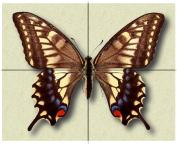
\includegraphics[width=0.75\textwidth]{butterfly.png}
\end{minipage}%\vspace{5pt}

\begin{esercizio}
\label{ese:8.26}
Perché la retta che congiunge i punti medi dei lati obliqui di un trapezio isoscele non è un suo asse di simmetria?
\end{esercizio}

\begin{esercizio}
\label{ese:8.27}
In $S_x$ (simmetria assiale rispetto all'asse $x$) il segmento $AB$ di estremi $A(3;2)$ e $B(3;-2)$
\begin{enumeratea}
\item è unito, luogo di punti uniti;
\item non ha punti fissi;
\item ha tutti i suoi punti uniti tranne $A$ e $B$;
\item ha un solo punto fisso;
\item ha solo $A$ e $B$ fissi.
\end{enumeratea}
\end{esercizio}

\begin{esercizio}
\label{ese:8.28}
Dimostrate che un qualunque segmento $MN$ di estremi $M(a;b)$ e $N(c;d)$ ha come corrispondente sia nella simmetria avente come asse l'asse $x$, sia nella simmetria avente come asse l'asse $y$, il segmento $M'N'$ tale che $MN\cong M'N'$.\vspace{5pt}

\noindent Ipotesi: $M(a;b)$, $N(c;d)$, $S_x:(M\rightarrow M') \wedge (N\rightarrow N')$\\
Tesi: $MN\cong M'N'$\vspace{3pt}\\
\emph{Dimostrazione.}\\
Determino $\overline{MN}=\ldots{}$ Trovo $M'(\ldots{};\ldots{})$ e $N'(\ldots{};\ldots{})$. Determino $\overline{M'N'}=\ldots{}$\\
Concludo: \ldots{}\vspace{5pt}

\noindent Ipotesi: $M(a;b)$, $N(c;d)$, $S_y:(M\rightarrow M') \wedge (N\rightarrow N')$\\
Tesi: $MN\cong M'N'$\vspace{3pt}\\
\emph{Dimostrazione.}\\
Determino $\overline{MN}=\ldots{}$ Trovo $M'(\ldots{};\ldots{})$ e $N'(\ldots{};\ldots{})$. Determino $\overline{M'N'}=\ldots{}$\\
Concludo: \ldots{}
\end{esercizio}

\begin{esercizio}
\label{ese:8.29} % 33
Il triangolo $ABC$ è isoscele; sapendo che $A(0;4)$, $B(-2;0)$ e che l'asse $x$ è il suo asse di simmetria, determinate il vertice $C$, il perimetro e l'area del triangolo.
\end{esercizio}

\begin{esercizio}
\label{ese:8.30} % 34
Il triangolo $ABC$ è isoscele; sapendo che $A(0;4)$, $B(-2;0)$ e che l'asse $y$ è il suo asse di simmetria, determinate il vertice $C$, il perimetro e l'area del triangolo.
\end{esercizio}

\noindent\begin{minipage}{0.45\textwidth}\parindent15pt
\begin{esercizio}
\label{ese:8.31} % 35
Considerate la funzione di proporzionalità quadratica $y=2x^2$. Rappresentatela nel riferimento cartesiano e segnate i suoi punti $A$, $B$ e $C$, rispettivamente di ascissa $x_A=1$, $x_B=-\frac{1}{2}$ e $x_C=\frac{1}{\sqrt{2}}$; trovate i corrispondenti $A'$, $B'$, $C'$ nella simmetria $S_y$ e verificate che appartengono alla funzione assegnata. Vi è un punto della curva rappresentata che risulta fisso in $S_y$? Inoltre, quale delle seguenti affermazioni ritenete corretta:
\begin{enumeratea}
\item la curva è fissa nella simmetria considerata;
\item la curva è unita nella simmetria considerata.
\end{enumeratea}
\end{esercizio}
\end{minipage}\hfil
\begin{minipage}{0.55\textwidth}
	\centering% (c) 2014 Daniele Masini - d.masini.it@gmail.com
\begin{tikzpicture}[scale=1,font=\small, x=5.9mm, y=5.9mm, smooth]
\usetikzlibrary{calc}

\begin{scope}

\begin{scope}[dotted,orange]
\draw[step=5.9mm] (-5.5,-5.5) grid (5.7,5.7);
\end{scope}

\begin{scope}[->]
\draw (-5.5,0) -- (5.7,0) node [below] {$x$};
\draw (0,-5.5) -- (0,5.7) node [left] {$y$};
\end{scope}

\foreach \x in {-5, -4, -3, -2, -1, 1, 2, 3, 4, 5}
\draw (\x,1.5pt) -- (\x,-1.5pt) node[below] {$\x$};

\foreach \y in {-5, -4, -3, -2, -1, 1, 2, 3, 4, 5}
\draw (1.5pt,\y) -- (-1.5pt,\y) node[left] {$\y$};

\node[below left] at (0,0) {O};
%\filldraw[fill=white, draw=black] (0,0) circle (2pt);

\end{scope}


\end{tikzpicture}

\end{minipage}\vspace{4pt}

\begin{esercizio}
\label{ese:8.32} % 38
I punti $A(-5;1)$, $B(-2;6)$, $C(3;6)$ e $D(0;1)$ sono vertici di un quadrilatero.
\begin{enumeratea}
\item Dimostrate che è un parallelogrammo.
\item Determinate perimetro e area;
\item Determinate la sua immagine $A'B'C'D'$ in $S_{y=3}$.
\end{enumeratea}
\`E vero che sia sul lato $AB$ che sul lato $CD$ esiste un punto fisso nella simmetria considerata? Tali punti su quali lati di $A'B'C'D'$ si trovano? Perché?
\end{esercizio}

\begin{esercizio}
\label{ese:8.33} % 40
Determinate l'immagine del quadrilatero $ABCD$ di vertici $A(0;0)$, $B(2;2)$, $C(5;3)$, $D(0;5)$ nella simmetria $S_{b1}$.
\end{esercizio}

\begin{esercizio}
\label{ese:8.34} % 41
Nella simmetria $S_{b1}$ la retta $y=-x$ è fissa o unita?
\end{esercizio}

\begin{esercizio}
\label{ese:8.35} % 42
Motivate la verità della seguente proposizione: <<nella simmetria $S_{b2}$ l'immagine dell'asse $x$ è l'asse $y$>>. Viene mantenuto l'orientamento dell'asse $x$?
Completate: $S_{b2}:(\text{asse }x)\rightarrow (\text{asse } \ldots{})$ e $(\text{asse }y)\rightarrow(\ldots\ldots{})$
Analogamente: $S_{b1}:(\text{asse }x)\rightarrow (\text{asse } \ldots{})$ e $(\text{asse }y)\rightarrow(\ldots\ldots{})$
\end{esercizio}

\begin{esercizio}
\label{ese:8.36} % 43
Dato il quadrilatero $ABCD$ di vertici $A(0;0)$, $B(3;1)$, $C(4;4)$ e $D(1;3)$ trovate il suo corrispondente in $S_{b1}$. Quale delle seguenti affermazioni ritenete corretta:
\begin{enumeratea}
\item il quadrilatero è fisso nella simmetria considerata;
\item il quadrilatero è unito nella simmetria considerata.
\end{enumeratea}
\end{esercizio}

\begin{esercizio}
\label{ese:8.37} % 44
Determinate il corrispondente del parallelogramma $ABCD$ di vertici $A(-5;1)$, $B(-2;6)$, $C(3;6)$, $D(0;1)$ in $S_{b1}$; perché $AA'$, $BB'$, $CC'$ e $DD'$ sono paralleli? Ricordando che il parallelogramma ha un centro di simmetria, determinate il centro di simmetria di $ABCD$ e verificate che in $S_{b1}$ esso ha come immagine il centro di simmetria di $A'B'C'D'$.
\end{esercizio}

\begin{esercizio}
\label{ese:8.38} % 45
Nel piano cartesiano sono assegnati i punti $A(0;3)$, $B(-2;0)$ e $C(-1;-3)$.
\begin{enumeratea}
\item Determinate i punti $A'$, $B'$ e $C'$ immagine in $S_{b2}$.
\item Calcolate l'area del quadrilatero $A'B'C'O$, essendo $O$ l'origine del riferimento.
\item Motivate la verità della proposizione: <<i segmenti $AB$ e $A'B'$ si incontrano in un punto $P$ della bisettrice del II\textsuperscript{o}-IV\textsuperscript{o} quadrante>>.
\item \`E vero che $AP'B$ è congruente a $PAB'$?
\end{enumeratea}
\end{esercizio}

\begin{esercizio}
\label{ese:8.39} % 46
Sono assegnate le simmetrie
\[S_1:\begin{cases}x'=-x\\y'=-y\end{cases};\quad S_2:\begin{cases}x'=y\\y'=x\end{cases};\quad
S_3:\begin{cases}x'=2-x\\y'=y\end{cases};\quad S_4:\begin{cases}x'=-x-1\\y'=3-y\end{cases}\]
Usando qualche punto scelto arbitrariamente riconosci ciascuna di esse e completa la tabella sottostante:
\begin{center}
\begin{tabular}{cccc}
\toprule
Simmetria & Tipo & Centro (coordinate) & Asse (equazione)\\
\midrule
$S_1$ & \ldots\ldots\ldots{} & \ldots\ldots{} & \ldots\ldots\ldots{} \\
$S_2$ & \ldots\ldots\ldots{} & \ldots\ldots{} & \ldots\ldots\ldots{} \\
$S_3$ & \ldots\ldots\ldots{} & \ldots\ldots{} & \ldots\ldots\ldots{} \\
$S_4$ & \ldots\ldots\ldots{} & \ldots\ldots{} & \ldots\ldots\ldots{} \\
\bottomrule
\end{tabular}
\end{center}
\end{esercizio}

\begin{esercizio}
\label{ese:8.40} % 47
Quale tra le seguenti caratteristiche è invariante in una simmetria assiale?
\begin{enumeratea}
\item la posizione della figura;
\item la direzione della retta;
\item il parallelismo;
\item l'orientamento dei punti;
\item dipende dall'asse di simmetria.
\end{enumeratea}
\end{esercizio}

\begin{esercizio}
\label{ese:8.41} % 48
I segmenti $AB$ e $A'B'$ si corrispondono nella simmetria di asse $r$; sapendo che $ABB'A'$ è un rettangolo, quale proposizione è vera?
\begin{enumeratea}
\item $AB$ è perpendicolare ad $r$;
\item $AB$ è parallelo ad $r$;
\item $AB$ appartiene ad $r$;
\item $AB$ è obliquo rispetto ad $r$ e $AB\cap r=H$.
\end{enumeratea}
\end{esercizio}

\begin{esercizio}
\label{ese:8.42} % 49
\`E assegnato il punto $P\left(-\sqrt{3};\dfrac{\sqrt{2}-1}{2}\right)$. Determinate il suo corrispondente nelle simmetrie indicate e completate:
\begin{center}
\begin{tabular}{ccc}
$S_{b2}:P\rightarrow P'(\ldots{};\ldots{})$ & $S_{x=-\frac{1}{2}}:P\rightarrow P'(\ldots{};\ldots{})$ & $S_{O}:P\rightarrow P'(\ldots{};\ldots{})$\\
$S_{x}:P\rightarrow P'(\ldots{};\ldots{})$ & $S_{y=2}:P\rightarrow P'(\ldots{};\ldots{})$ & $S_{C(1;1)}:P\rightarrow P'(\ldots{};\ldots{})$\\
\end{tabular}
\end{center}
\end{esercizio}

\begin{esercizio}
\label{ese:8.43} % 50
Un segmento unito in $S_{b2}$ è
\begin{enumeratea}
\item un segmento perpendicolare alla bisettrice del I\textsuperscript{o}-III\textsuperscript{o} quadrante;
\item un segmento perpendicolare alla bisettrice del II\textsuperscript{o}-IV\textsuperscript{o} quadrante nel suo punto medio;
\item un segmento parallelo alla bisettrice del I\textsuperscript{o}-III\textsuperscript{o} quadrante;
\item un segmento perpendicolare alla bisettrice del II\textsuperscript{o}-IV\textsuperscript{o} quadrante;
\item un segmento avente il suo punto medio appartenente alla bisettrice del II\textsuperscript{o}-IV\textsuperscript{o} quadrante.
\end{enumeratea}
\end{esercizio}

\noindent\begin{minipage}{0.75\textwidth}\parindent15pt
\begin{esercizio}
\label{ese:8.44} % 51
Nel piano sono assegnati i tre punti $A$, $B$ e $A'$ dei quali il punto $A'$ è immagine di $A$ in una traslazione. Dopo aver determinato il vettore della traslazione costruite l'immagine del triangolo $ABA'$.
\end{esercizio}
\end{minipage}\hfil
\begin{minipage}{0.25\textwidth}
	\centering~~% (c) 2014 Daniele Masini - d.masini.it@gmail.com
\begin{tikzpicture}[scale=1,font=\small]
\usetikzlibrary{calc}

\begin{scope}
\draw[fill] (0,0) circle (1pt) node[above right] {$B$};
\draw[fill] (0,1.2) circle (1pt) node[above right] {$A$};
\draw[fill] (1.8,0) circle (1pt) node[above right] {$A'$};
\end{scope}

\end{tikzpicture}

\end{minipage}\vspace{8pt}

\begin{esercizio}
\label{ese:8.45} % 52
Determinate l'immagine del parallelogrammo $ABCD$ nella traslazione di vettore $\vec{v} \equiv \overrightarrow{AC}$.
\end{esercizio}

\noindent\begin{minipage}{0.75\textwidth}\parindent15pt
\begin{esercizio}
\label{ese:8.46} % 53
Dati due punti distinti $A$ e $B$ e il vettore $\overrightarrow{CD}$ della figura a fianco, detti $A'$ e $B'$ i punti immagine di $A$ e $B$ nella traslazione di vettore $\overrightarrow{CD}$, rispondete alle domande:
\begin{enumeratea}
\item Di che natura è il quadrilatero $ABB'A'$?
\item Può succedere che il quadrilatero in questione sia un rettangolo? E un rombo?
\item Cosa succede se $AB$ è parallelo al vettore $\overrightarrow{CD}$?
\end{enumeratea}
\end{esercizio}
\end{minipage}\hfil
\begin{minipage}{0.25\textwidth}
	\centering~~% (c) 2014 Daniele Masini - d.masini.it@gmail.com
\begin{tikzpicture}[scale=1,font=\small]
\usetikzlibrary{calc}

\begin{scope}
\draw[fill] (0,0) coordinate (c) circle (1pt) node[above right] {$C$};
\draw[fill] (1.7,0) coordinate (d) circle (1pt) node[above right] {$D$};
\draw[thick, blue, ->] (c) -- (d);
\draw[fill] (-0.4,-0.8) coordinate (a) circle (1pt) node[above right] {$A$};
\draw[fill] (0.7,-1.7) coordinate (b) circle (1pt) node[above right] {$B$};
\end{scope}

\end{tikzpicture}

\end{minipage}\vspace{8pt}

\begin{esercizio}
\label{ese:8.47} % 54
Come dobbiamo assegnare due segmenti $AB$ e $A'B'$ affinché siano corrispondenti in una traslazione? \`E unica la traslazione che associa ad $AB$ il segmento $A'B'$?
\end{esercizio}

\begin{esercizio}
\label{ese:8.48} % 58
Nel riferimento cartesiano è assegnato il punto $P(-4;2)$. Determinate il punto $P'$ immagine nella traslazione $T(3;-1):\begin{cases}x'=x+3\\y'=y+(-1)\end{cases}$.\\
Strategia risolutiva:
\begin{enumerate*}
\item individuate il vettore $\vec{w}$ della traslazione: $\vec{w}(\ldots{};\ldots{})$;
\item tracciate il vettore nel riferimento cartesiano;
\item determinate le coordinate di $P'$: $P'(\ldots{};\ldots{})$.
\end{enumerate*}
Completate: $\overrightarrow{PP'}$ è \ldots\ldots\ldots{} a $\vec{w}$; questo significa che i due vettori hanno \ldots\ldots\ldots{} direzione (cioè sono \ldots\ldots\ldots{}), stesso \ldots\ldots\ldots{} e \ldots\ldots\ldots{} intensità.
\end{esercizio}

\begin{esercizio}
\label{ese:8.49} % 59
Nel riferimento cartesiano, dopo aver fissato il punto $P(-4;2)$ siano dati i punti $Q(\ldots{};\ldots{})$ e $Q'(\ldots{};\ldots{})$ immagine nella traslazione $T(3;-1)$. Dimostrate con le conoscenze di geometria sintetica che $PP'Q'Q$ è un parallelogramma.\vspace{5pt}\\
\noindent Ipotesi: $PP'\cong QQ'$, $PP'\ldots{}QQ'$\\
Tesi: \ldots\ldots\ldots{}\vspace{3pt}\\
\emph{Dimostrazione. \ldots\ldots{}}
\end{esercizio}

\begin{esercizio}
\label{ese:8.50} % 60
Sappiamo che l'equazione di una traslazione è $T(a;b):\begin{cases}x'=x+a\\y'=y+b\end{cases}$. Assegnate le coordinate $(x;y)$ di un punto $P$ e $(x';y')$ della sua immagine $P'$, le componenti del vettore della traslazione sono date da:
\begin{multicols}{2}
\begin{enumeratea}
\item $a=x'+x$\quad e\quad $b=y'+y$;
\item $a=x-x'$\quad e\quad $b=y-y'$;
\item $a=x'-x$\quad e\quad $b=y'-y$;
\item $a=x'+x$\quad e\quad $b=y'-y$;
\item $a=\dfrac{x'}{x}$\quad e\quad $b=\dfrac{y'}{y}$.
\end{enumeratea}
\end{multicols}
\end{esercizio}


\begin{esercizio}
\label{ese:8.51} % 61
Dopo aver determinato l'equazione della traslazione in cui $A'(0;-2)$ è l'immagine di $A(3;2)$, determinate il perimetro del triangolo $AO'A'$ essendo $O'$ il corrispondente di $O(0;0)$ nella traslazione trovata.
\end{esercizio}

\begin{esercizio}
\label{ese:8.52} % 62
Verificate che il punto medio $M$ del segmento $PQ$ di estremi $P(-1;4)$ e $Q(5;0)$ ha come immagine in $T(3;-1)$ il punto medio $M'$ del segmento $P'Q'$.
\end{esercizio}

\begin{esercizio}
\label{ese:8.53} % 63
Applica la traslazione di equazione $\begin{cases}x'=x+2\\y'=y-1\end{cases}$ al segmento di estremi $A(-2;4)$ e $B(3;3)$. 
\end{esercizio}

\begin{esercizio}
\label{ese:8.54} % 64
Dati $A(1;0)$ e $B(0;2)$, determina $C$ e $D$ in modo che $ABCD$ sia un quadrato.
\end{esercizio}

\begin{esercizio}
\label{ese:8.55} % 65
Determinate l'immagine del triangolo di vertici $A(0;2)$, $B(-3;2)$ e $C(0;5)$ nella traslazione $T(4;1)$. Calcolatene quindi perimetro e area.
\end{esercizio}

\begin{esercizio}
\label{ese:8.56} % 66
Determinate l'equazione della traslazione di vettore $\vec{s}=\vec{u}+\vec{v}$ assegnati dalla figura~\ref{fig:ese8.56}. Determinate inoltre l'immagine del poligono di vertici $H(-1;1)$, $K(0;-2)$, $L(3;0)$ ed $F(1;2)$.
\end{esercizio}

\begin{figure}[!htb]
	\centering% (c) 2014 Daniele Masini - d.masini.it@gmail.com
\begin{tikzpicture}[scale=1,font=\small, x=6.3mm, y=6.3mm, smooth]
\usetikzlibrary{calc}

\begin{scope}

\begin{scope}[dotted,orange]
\draw[step=6.3mm] (-2.5,-2.5) grid (7.7,2.7);
\end{scope}

\begin{scope}[->]
\draw (-2.5,0) -- (7.7,0) node [below] {$x$};
\draw (0,-2.5) -- (0,2.7) node [left] {$y$};
\end{scope}

\foreach \x in {-2, -1, 1, 2, 3, 4, 5, 6, 7}
\draw (\x,1.5pt) -- (\x,-1.5pt) node[below] {$\x$};

\foreach \y in {-2, -1, 1, 2}
\draw (1.5pt,\y) -- (-1.5pt,\y) node[left] {$\y$};

\node[below left] at (0,0) {O};
%\filldraw[fill=white, draw=black] (0,0) circle (2pt);

\draw[thick, blue, ->] (0,0) -- node [black, above] {$\vec{u}$} (3,2);
\draw[thick, blue, ->] (0,0) -- node [black, shift={(-0.2,-0.45)}] {$\vec{v}$} (1,-2);

\end{scope}


\end{tikzpicture}

	\caption{Esercizio~\ref{ese:8.56}}\label{fig:ese8.56}
\end{figure}\vspace{8pt}

\begin{esercizio}
\label{ese:8.57} % 67
Un vettore $\vec{v}$ ha modulo unitario, è applicato nell'origine $O$ e forma con l'asse delle ascisse un angolo di $30\grado$. Determinate le sue componenti e scrivete l'equazione della traslazione da esso caratterizzata.
\end{esercizio}

\noindent\begin{minipage}{0.7\textwidth}\parindent15pt
\begin{esercizio}
\label{ese:8.58} % 68
Prendete in considerazione l'angolo $\epsilon$ di vertice $T$ della figura a fianco. Sia $O$ il centro di rotazione e $F$ un punto del piano di cui si vuole determinare l'immagine. Costruite $F'$ seguendo i passi illustrati immediatamente dopo la definizione~\ref{def:rotaz} a pagina~\pageref{def:rotaz}.
\end{esercizio}
\end{minipage}\hfil
\begin{minipage}{0.3\textwidth}
	\centering~~% Copyright (c) 2015 Daniele Masini - d.masini.it@gmail.com

\begin{tikzpicture}[scale=1,font=\small, x=6.3mm, y=6.3mm, smooth]
\usetikzlibrary{calc}

\begin{scope}
\coordinate (t) at (0,0);
\coordinate (f) at (3,0);
\coordinate (o) at (3,-1.5);
\path (t) -- +(20:2) coordinate (t1);
\path (t) -- +(150:2) coordinate (t2);

\begin{scope}
\clip (t1) -- (t) -- (t2) -- cycle;
\draw[blue, fill=blue!10] (t) circle (0.4) node [black, shift={(90:0.6)}] {$\epsilon$};
\end{scope}

\draw (t) -- node[shift={(0.3,-0.25)}] {$t$} (t1);
\draw (t) -- node[shift={(-0.3,-0.3)}] {$p$} (t2);

\draw[fill] (t) circle (1pt) node [below] {$T$};
\draw[fill] (f) circle (1pt) node [above right] {$F$};
\draw[fill] (o) circle (1pt) node [above right] {$O$};

\end{scope}


\end{tikzpicture}

\end{minipage}\vspace{8pt}

\begin{esercizio}
\label{ese:8.59} % 69
Costruite l'immagine del quadrato $ABCD$ nella rotazione di $+90\grado$ avente come centro di simmetria il vertice $B$.
Fissate i punti medi $M$ ed $N$ rispettivamente di $AB$ e di $CD$; dove si trovano le rispettive immagini?
\end{esercizio}

\begin{esercizio}
\label{ese:8.60} % 70
\`E vero che il quadrato è unito nella rotazione avente come centro il punto di incontro delle diagonali e come ampiezza $90\grado$?
\end{esercizio}

\begin{esercizio}
\label{ese:8.61} % 71
L'ortocentro di un triangolo equilatero è il centro di una rotazione in cui il triangolo è unito. Determinate l'angolo di rotazione.
\end{esercizio}

\begin{esercizio}
\label{ese:8.62} % 72
Costruite l'immagine $A'B'C'$ del triangolo equilatero $ABC$ nella rotazione di centro $B$ e ampiezza $-120\grado$. Dimostrate che $C$, $B$ ed $A'$ sono allineati e che $ABC'$ è un triangolo equilatero congruente a quello dato.
\end{esercizio}

\noindent\begin{minipage}{0.75\textwidth}\parindent15pt
\begin{esercizio}
\label{ese:8.63} % 73
Nel piano è assegnato il punto $C$ e il vettore $\vec{v}$ (figura a lato); costruite l'immagine del punto $P$ nell'isometria $T_{\vec{v}} \circ S_{C}$ e anche l'immagine dello stesso punto $P$ nell'isometria $S_{C} \circ T_{\vec{v}}$. Determinate l'equazione di $\Phi_1 = T_{\vec{v}} \circ S_{C}$ e di $\Phi_2 = S_{C} \circ T_{\vec{v}}$.
\end{esercizio}
\end{minipage}\hfil
\begin{minipage}{0.25\textwidth}
	\centering~~% (c) 2014 Daniele Masini - d.masini.it@gmail.com
\begin{tikzpicture}[scale=1,font=\small, x=6.3mm, y=6.3mm, smooth]
\usetikzlibrary{calc}

\begin{scope}
\coordinate (v) at (0,0);
\coordinate (c) at (1.8,2);
\coordinate (p) at (-.2,2.3);
\path (v) -- +(15:2.5) coordinate (v1);

\draw[blue, thick, ->] (v) -- node [black, above] {$\vec{v}$} (v1);

\draw[fill] (v) circle (1pt);
\draw[fill] (c) circle (1pt) node [above right] {$C$};
\draw[fill] (p) circle (1pt) node [above right] {$P$};

\end{scope}


\end{tikzpicture}

\end{minipage}\vspace{8pt}

\begin{esercizio}
\label{ese:8.64} % 74
Il centro della simmetria è il punto $C(-1;-2)$, il vettore della traslazione è $\vec{v}(3;-2)$ e il punto di cui vogliamo determinare l'immagine è scelto da voi arbitrariamente. 
\end{esercizio}

\begin{esercizio}
\label{ese:8.65} % 75
Sono assegnati il punto $C(-4;3)$, la retta $x=1$ e il punto $P(0;5)$. Determinate l'immagine $P''$ di $P$ nell'isometria $\Delta=S_{C}\circ S_{x=1}$ e l'immagine $P^*$ di $P$ nell'isometria $\Delta=S_{x=1}\circ S_{C}$. \`E vero che $P''$ e $P^*$ si corrispondono nella simmetria $S_y$? Determinate l'area del triangolo $PP''P^*$.
\end{esercizio}

\begin{esercizio}
\label{ese:8.66} % 76
\`E assegnato un punto $O$; determinate l'immagine $P'$ di un punto $P$ nella rotazione di centro $O$ e angolo di $60\grado$ e l'immagine $P''$ di $P'$ nella simmetria avente come asse la retta $PO$.
\begin{enumeratea}
\item Completate: $P \overset{\ldots{}}\longrightarrow P'$. 
\item Dimostrate che $P$, $P'$ e $P''$ appartengono alla circonferenza di centro $O$ e raggio $OP$.
\item Individuate le caratteristiche del quadrilatero $PP''OP'$.
\item Determinatene l'area, supponendo $\overline{OP}=2$~m.
\end{enumeratea}
\end{esercizio}

\begin{esercizio}
\label{ese:8.67} % 80
$ABC$ è un triangolo equilatero e $O$ è il centro della sua circonferenza circoscritta. Dimostrate che il triangolo è unito nella rotazione di centro $O$ e angolo $\alpha=120\grado$. Analogamente il quadrato $ABCD$ è unito nella rotazione di centro $H$, punto di incontro delle sue diagonali, di angolo $\alpha=90\grado$.
\end{esercizio}

\begin{esercizio}
\label{ese:8.68} % 81
Giustificate la verità della proposizione: <<La simmetria centrale di centro $K$ è una rotazione di $180\grado$>>.
\end{esercizio}

\begin{esercizio}
\label{ese:8.69} % 82
Nel piano dotato di riferimento cartesiano è tracciata la bisettrice del I\textsuperscript{o} e III\textsuperscript{o} quadrante e la retta $y=1$. Completate le osservazioni seguenti:
\begin{enumeratea}
\item il punto di intersezione $K$ ha coordinate $K(\ldots{};\ldots{})$;
\item l'angolo delle due rette è di $\ldots{}\grado$.
\end{enumeratea}
\end{esercizio}

\begin{esercizio}
\label{ese:8.70} % 83
Scrivete l'equazione della simmetria avente come asse la bisettrice: $S_{b1}\begin{cases}x'=\ldots{}\\y'=\ldots{}\end{cases}$ e l'equazione della simmetria di asse la retta $y=1$: $S_{y=1}\begin{cases}x'=\ldots{}\\y'=\ldots{}\end{cases}$.
\end{esercizio}

\begin{esercizio}
\label{ese:8.71} % 84
Determinate le coordinate del punto $P''$ immagine di $P$, arbitrariamente scelto, in $\Omega = S_{b1} \circ S_{y=1}$ e scrivete l'equazione di $\Omega$.
Concludete: $\Omega$ è la rotazione di centro \ldots{} e angolo \ldots{} (ricordate il segno dell'angolo di rotazione).
\end{esercizio}

\begin{esercizio}
\label{ese:8.72} % 85
Determinate le coordinate del punto $P^*$ immagine di $P$, arbitrariamente scelto, in $\Omega^*=S_{y=1} \circ S_{b1}$ e scrivete l'equazione di $\Omega^*$.
Concludete: $\Omega^*$ è la rotazione di centro \ldots{} e angolo \ldots{} (ricordate il segno dell'angolo di rotazione).
\end{esercizio}

\begin{esercizio}
\label{ese:8.73} % 86
Determinate l'equazione della isometria $J=S_{b1} \circ S_{x=4}$ e stabilite se esiste qualche elemento unito. Come cambia l'equazione dell'isometria $J^*=S_{x=4} \circ S_{b1}$ rispetto alla precedente? Sia $J$ che $J^*$ sono rotazioni: determinate centro e angolo (con segno) di ognuna di esse. A questo scopo potete utilizzare il punto $P(2;4)$ o un punto arbitrariamente scelto.
\end{esercizio}

\noindent\begin{minipage}{0.7\textwidth}\parindent15pt
\begin{esercizio}
\label{ese:8.74} % 87
Determinate l'immagine del punto $A$ nell'isometria $\Delta=S_b \circ S_a$ essendo $a$ e $b$ le rette parallele segnate nella figura a fianco e $A$ il punto dato. Dimostrate che $\overline{AA''}=2\cdot d$ essendo $d$ la distanza tra le rette $a$ e $b$.
Fissate arbitrariamente un altro punto $B$ non appartenente ad alcuna delle rette date e determinate la sua immagine $B''$ nell'isometria $\Delta$.
\`E vero che $\overline{AA''}=\overline{BB''}$ e $\overline{AA''} \parallel \overline{BB''}$? Potete concludere che l'isometria $\Delta$ è la traslazione di vettore $\overrightarrow{AA''}$?
\end{esercizio}
\end{minipage}\hfil
\begin{minipage}{0.3\textwidth}
	\centering~~% Copyright (c) 2015 Daniele Masini - d.masini.it@gmail.com

\begin{tikzpicture}[scale=1,font=\small]
\usetikzlibrary{calc}

\begin{scope}
\coordinate (a) at (0,0);

\draw[blue, thick] (-1.5,-0.5) -- (1.5,-0.5) node [black, above] {$a$};
\draw[blue, thick] (-1.5,-1.5) -- (1.5,-1.5) node [black, above] {$b$};

\draw[fill] (a) circle (1pt) node [above right] {$A$};

\end{scope}


\end{tikzpicture}


\end{minipage}\vspace{8pt}

\begin{esercizio}
\label{ese:8.75} % 88
Facendo riferimento all'esercizio~\ref{ese:8.74}, verificate che la traslazione $\Delta_1 = S_a \circ S_b$ è caratterizzata da un vettore avente modulo e direzione uguali al vettore $\overrightarrow{AA''}$ ma verso opposto.
\end{esercizio}

\begin{esercizio}
\label{ese:8.76} % 89
Nel riferimento cartesiano ortogonale sono assegnati i punti $A(1;5)$, $B(2;1)$ e $C(-1;3)$. Determinate i punti $A''$, $B''$ e $C''$ immagine rispettivamente di $A$, $B$ e $C$ nella traslazione $T=S_{x=-2} \circ S_{x=1}$. Scrivete l'equazione della traslazione, individuate il vettore che la definisce calcolandone modulo e direzione.
\end{esercizio}

\begin{esercizio}
\label{ese:8.77} % 90
Determinate i vettori $\vec{u}$ e $\vec{v}$ delle traslazioni $T_{\vec{u}}\begin{cases}x'=x+1\\y'=y-2\end{cases}$ e $T_{\vec{v}}\begin{cases}x'=x-3\\y'=y-1\end{cases}$ e il vettore $\vec{s} = \vec{u} + \vec{v}$. Verificate che $T_{\vec{s}} = T_{\vec{u}} \circ T_{\vec{v}}$.
Cosa otteniamo dalla composizione $T_{\vec{u}} \circ T_{\vec{v}}$? Sapresti darne la motivazione?
Concludete: componendo due traslazioni si ottiene \ldots\ldots{}
\end{esercizio}

\begin{esercizio}
\label{ese:8.78} % 91
Nel riferimento cartesiano ortogonale $Oxy$ è assegnato il punto $O_1(2;1)$; scrivete l'equazione della simmetria centrale di centro $O$ $S_O\begin{cases}x'=\ldots{}\\y'=\ldots{}\end{cases}$  e l'equazione della simmetria centrale di centro $O_1$ $S_{O_1}\begin{cases}x'=\ldots{}\\y'=\ldots{}\end{cases}$. Determinate l'immagine $P''$ del punto $P(1;2)$ nell'isometria $\Sigma=S_O \circ S_{O_1}$ di cui avrete scritto l'equazione e determinate $\overline{PP''}$. Determinate $Q''$ immagine di $Q\left(\frac{1}{2};-1\right)$ nell'isometria $\Sigma$ e determinate $\overline{QQ''}$. Potete affermare che $\overrightarrow{PP''} \equiv \overrightarrow{QQ''}$? Verificate che $\overrightarrow{PP''} \equiv \overrightarrow{QQ''} \equiv 2\cdot \overrightarrow{O_1O}$.
\`E vero che $\Sigma=S_O \circ S_{O_1}$ e $\Sigma_1=S_{O_1} \circ S_{O}$ sono la stessa isometria?
\end{esercizio}

\begin{esercizio}
\label{ese:8.79} % 93
Dimostrate che la composizione di due simmetrie centrali è una traslazione caratterizzata dal vettore parallelo alla retta passante per i due centri e modulo uguale al doppio della loro distanza.
\end{esercizio}

\begin{esercizio}
\label{ese:8.80} % 94
Si consideri la composizione di due simmetrie assiali con assi paralleli $S_b\begin{cases}x'=2b-x\\y'=y\end{cases}$ e $S_a\begin{cases}x'=a-x\\y'=y\end{cases}$.
Componendo le due simmetrie si ha $S_b\begin{cases}x'=2b-2a+x\\y'=y\end{cases}$ che è \ldots\ldots{}
Se $a=b$ le due simmetrie sono \ldots\ldots{} la loro composizione è \ldots\dots{}
\end{esercizio}

\begin{esercizio}
\label{ese:8.81} % 95
Si consideri la composizione di due simmetrie assiali con assi perpendicolari.
Una simmetria con asse parallelo all'asse $y$ ha equazione $S_a\begin{cases}x'=2a-x\\y'=y\end{cases}$ e asse $x = a$.
Mentre una simmetria con asse parallelo all'asse $x$ ha equazione $S_b\begin{cases}x'=x\\y'=2b-y\end{cases}$ e asse $y = b$.
Componendo le due simmetrie otteniamo \ldots\ldots{}
\end{esercizio}

\begin{esercizio}
\label{ese:8.82} % 96
Verificate che:
\begin{enumeratea}
\item l'inversa della traslazione di vettore $\vec{v}(a;b)$ è la traslazione di vettore $-\vec{v}$;
\item l'inversa di una rotazione di centro $O$ e angolo $\alpha$ è la rotazione di centro $O$ e angolo $-\alpha$.
\end{enumeratea}
\end{esercizio}

\begin{esercizio}
\label{ese:8.83} % 97
Verificate che le simmetrie (centrale e assiale) hanno se stesse come isometria inversa, ossia $(S_K)^{-1}=S_K$ e $(S_r)^{-1}=S_r$.
\end{esercizio}

\begin{esercizio}
\label{ese:8.84} % 98
La proposizione <<la simmetria centrale è la composizione di due simmetrie assiali>> è:
\begin{enumeratea}
\item sempre vera;
\item vera se i due assi sono incidenti;
\item mai vera;
\item vera se i due assi sono perpendicolari;
\item vera se i due assi sono paralleli.
\end{enumeratea}
\end{esercizio}

\begin{esercizio}
\label{ese:8.85} % 99
Completa la proposizione: <<la simmetria centrale di centro $C\left(-\frac{5}{3};\sqrt{3}\right)$ può essere ottenuta come composizione delle due simmetrie assiali di assi le rette \ldots\ldots{} e \ldots\ldots{} e la sua equazione è \ldots\ldots\ldots{}
\end{esercizio}

\begin{esercizio}
\label{ese:8.86} % 100
Stabilite il valore di verità delle proposizioni:
%Componendo due isometrie si ottiene una isometria
\begin{enumeratea}
\item Componendo due simmetrie assiali si ottiene una simmetria assiale\hfill\boxV\quad\boxF
\item Componendo due traslazioni si ottiene una traslazione\hfill\boxV\quad\boxF
\item Componendo due simmetrie centrali si ottiene una simmetria centrale\hfill\boxV\quad\boxF
\item Componendo due simmetrie assiali di assi incidenti si ottiene una rotazione\hfill\boxV\quad\boxF
\item Componendo due rotazioni si ottiene una rotazione\hfill\boxV\quad\boxF
\item L'identità si ottiene componendo una isometria con sé stessa\hfill\boxV\quad\boxF
\item L'inversa di una traslazione è la stessa traslazione\hfill\boxV\quad\boxF
\item Componendo una simmetria centrale con una rotazione si ottiene l'identità\hfill\boxV\quad\boxF
\item Componendo una simmetria centrale di centro $H$ con la simmetria assiale avente come asse una retta passante per $H$ si ottiene sempre l'identità\hfill\boxV\quad\boxF
\end{enumeratea}
\end{esercizio}

\begin{esercizio}
\label{ese:8.87} % 101
L'equazione $\begin{cases}x'=4-x\\y'=y\end{cases}$ descrive: 
\begin{enumeratea}
\item la simmetria assiale di asse $y$;
\item la simmetria assiale di asse la retta $x=4$;
\item la traslazione di vettore $\vec{v}(4;0)$;
\item la simmetria assiale di asse $x=2$;
\item la simmetria centrale di centro $C(4;0)$.
\end{enumeratea}
\end{esercizio}

\begin{esercizio}
\label{ese:8.88} % 102
La trasformazione $\Sigma \begin{cases}x'=-y+2\\y'=2x\end{cases}$ è un'isometria?
\end{esercizio}

\begin{esercizio}
\label{ese:8.89} % 103
Il segmento di estremi $A(3;4)$ e $B(3;-2)$ ha come simmetrico il segmento di estremi $A'(3;2)$ e $B'(5;2)$; è stata eseguita:
\begin{enumeratea}
\item la simmetria assiale di asse la retta $x=4$;
\item la simmetria $S_{b2}$;
\item la simmetria $S_{b1}$;
\item la simmetria assiale di asse la retta $x=3$;
\item la simmetria $S_{y=3}$.
\end{enumeratea}
\end{esercizio}

\begin{esercizio}
\label{ese:8.90} % 104
Attribuisci il valore di verità alle seguenti proposizioni:
\begin{enumeratea}
\item In una isometria vi è almeno un elemento unito\hfill\boxV\quad\boxF
\item Nella simmetria centrale vi sono infinite rette unite, ma solamente un punto unito\tab\tab\hfill\boxV\quad\boxF
\item In ogni triangolo vi è almeno un asse di simmetria\hfill\boxV\quad\boxF
\item Qualche quadrilatero ha un centro di simmetria\hfill\boxV\quad\boxF
\item Il triangolo equilatero ha un centro di simmetria\hfill\boxV\quad\boxF
\item Il rombo è l'unico quadrilatero avente due assi di simmetria\hfill\boxV\quad\boxF
\item Tutte le rette aventi la stessa direzione del vettore della traslazione sono rette unite\tab\tab\hfill\boxV\quad\boxF
\item Solo la simmetria assiale è una isometria invertente\hfill\boxV\quad\boxF
\item Rette parallele hanno come immagine in una isometria rette parallele\hfill\boxV\quad\boxF
\item In una isometria una retta è sempre parallela alla sua immagine\hfill\boxV\quad\boxF
\end{enumeratea}
\end{esercizio}

\begin{esercizio}
\label{ese:8.91} % 105
Il quadrilatero di vertici $A(5;0)$, $B(9;0)$, $C(12;4)$ e $D(7;3)$ nella simmetria $S_x$ ha fisso il lato $AB$. Spiegate come sia possibile questo fatto.
\end{esercizio}

\begin{esercizio}
\label{ese:8.92} % 106
Dimostrate che la bisettrice di un angolo è il suo asse di simmetria.
\end{esercizio}

\begin{esercizio}
\label{ese:8.93} % 107
Il rettangolo $ABCD$ con $AB<BC$ ha come immagine il rettangolo $A'B'C'D'$ nella simmetria avente come asse la retta $AC$. Potete affermare che $AB'DCD'B$ è un esagono regolare?
\end{esercizio}

\noindent\begin{minipage}{0.75\textwidth}\parindent15pt
\begin{esercizio}
\label{ese:8.94} % 108
I due segmenti della figura a fianco possono essere corrispondenti in una simmetria centrale? 
\end{esercizio}
\end{minipage}\hfil
\begin{minipage}{0.25\textwidth}
	\centering~~% Copyright (c) 2015 Daniele Masini - d.masini.it@gmail.com

\begin{tikzpicture}[scale=1,font=\small]
\usetikzlibrary{calc}

\begin{scope}
\coordinate (a) at (0,0);
\path (a) -- +(15:1.5) coordinate (b);
\coordinate (c) at (0.3,-1);
\path (c) -- +(0:1.5) coordinate (d);

\draw[thick] (a) -- node [below] {$a$} (b);
\draw[thick] (c) -- node [below] {$c$} (d);

\draw[fill] (a) circle (1pt) node [above] {$A$};
\draw[fill] (b) circle (1pt) node [above] {$B$};
\draw[fill] (c) circle (1pt) node [above] {$C$};
\draw[fill] (d) circle (1pt) node [above] {$D$};

\end{scope}


\end{tikzpicture}


\end{minipage}\vspace{8pt}

\noindent\begin{minipage}{0.65\textwidth}\parindent15pt
\begin{esercizio}
\label{ese:8.95} % 109
Nella figura a fianco abbiamo disegnato il quadrato $ABCD$ e il punto $A'$ corrispondente di $A$ in una isometria. Stabilite quale isometria è completamente fissata con questi elementi (simmetria assiale, traslazione, simmetria centrale) e determinate in essa l'immagine del quadrato. 
\end{esercizio}
\end{minipage}\hfil
\begin{minipage}{0.35\textwidth}
	\centering~~% (c) 2014 Daniele Masini - d.masini.it@gmail.com
\begin{tikzpicture}[scale=0.9,font=\small]
\usetikzlibrary{calc}

\begin{scope}
\coordinate (a) at (0,0);
\path (a) -- +(0:1.5) coordinate (b);
\path (b) -- +(270:1.5) coordinate (c);
\path (c) -- +(180:1.5) coordinate (d);
\coordinate (a1) at (4,-0.75);

\draw[thick] (a) -- (b) -- (c) -- (d) -- cycle;

\node[above left] at (a) {$A$};
\node[above right] at (b) {$B$};
\node[below right] at (c) {$C$};
\node[below left] at (d) {$D$};

\draw[fill] (a1) circle (1pt) node[above] {$A'$};

\end{scope}


\end{tikzpicture}


\end{minipage}\vspace{8pt}

\begin{esercizio}
\label{ese:8.96} % 110
Costruite l'immagine di un triangolo rettangolo $ABC$ (non isoscele) di ipotenusa $BC$
\begin{enumeratea}
\item in ciascuna delle simmetrie $S_A$, $S_B$ e $S_C$;
\item nella simmetria $S_M$ essendo $M$ il punto medio dell'ipotenusa;
\item in ciascuna delle simmetrie aventi come assi le rette dei lati.
\end{enumeratea}
\end{esercizio}

\begin{esercizio}
\label{ese:8.97} % 111
Comporre due traslazioni di vettori $\vec{v_1}(2;3)$ e $\vec{v_2}(3;6)$ applicandole al triangolo $ABC$ con $A(-2;-1)$, $B(-1;-2)$ e $C(-4;-3)$.
\end{esercizio}

\begin{esercizio}
\label{ese:8.98} % 112
Determina il corrispondente $A'B'$ del segmento di vertici $A(-2;6)$ e $B(-3;3)$ nella simmetria di asse $x=-1$. Applica poi al segmento ottenuto un'ulteriore simmetria con asse $x=4$. Utilizzando l'equazione per la composizione di due simmetrie con assi paralleli tra loro, trova le nuove coordinate dei due punti $A$ e $B$.
\end{esercizio}

\begin{esercizio}
\label{ese:8.99} % 113
Determina il corrispondente $A'B'$ del segmento di vertici $A(1;-6)$ e $B(4;3)$ nella simmetria di asse $x = 2$, applica poi al segmento ottenuto un'ulteriore simmetria con asse $y = 1$. Utilizzando l'equazione per la composizione di due simmetrie con assi perpendicolari tra loro, determina le nuove coordinate dei due punti $A$ e $B$.
\end{esercizio}

\begin{esercizio}
\label{ese:8.100} % 114
Componi le seguenti trasformazioni geometriche scrivendo l'equazione della trasformazione composta e fornendo un esempio con disegno relativo. 
\begin{enumeratea}
\item Due rotazioni con lo stesso centro.
\item Due rotazioni con centro diverso.
\item Due simmetrie centrali.
\item Due rotazioni di un angolo retto.
\end{enumeratea}
\end{esercizio}

\begin{esercizio}
\label{ese:8.101} % 115
Sono assegnate le simmetrie assiali
\[S_1 \begin{cases}x'=x\\y'=2-y\end{cases}\quad  S_2 \begin{cases}x'=-x\\y'=y\end{cases}\quad S_3 \begin{cases}x'=x\\y'=y\end{cases}\quad S_4 \begin{cases}x'=-x-6\\y'=y\end{cases}\]
\begin{enumeratea}
\item Individuate l'asse di simmetria di ciascuna di esse, rappresentate nel riferimento cartesiano ortogonale i rispettivi assi indicandoli con $s_1$, $s_2$, $s_3$ e $s_4$; completate e riproducete nello stesso riferimento

\begin{center}
\begin{tabular}{cc}
$P\left(-3;\frac{1}{2}\right)\overset{S_1}\longrightarrow P_1(\ldots{};\ldots{})$ & $P\left(-3;\frac{1}{2}\right)\overset{S_2}\longrightarrow P_2(\ldots{};\ldots{})$\\
$P\left(-3;\frac{1}{2}\right)\overset{S_3}\longrightarrow P_3(\ldots{};\ldots{})$ & $P\left(-3;\frac{1}{2}\right)\overset{S_4}\longrightarrow P_4(\ldots{};\ldots{})$\\
\end{tabular}
\end{center}

\item Siano $A$, $B$, $C$ e $D$ i punti $A=s_4\cap s_3$, $B=s_4\cap s_1$, $C=s_1\cap s_3$ e $D=s_2\cap s_1$; dimostrate che i triangoli $ABC$ e $CDE$ sono rettangoli isosceli e che i lati dell'uno sono il quadruplo di quelli dell'altro.
\item Determinate il rapporto tra i loro perimetri e tra le loro aree.
\end{enumeratea}
\end{esercizio}

%\end{multicols}

\subsection{Risposte}

\begingroup
\hypersetup{linkcolor=black}

\paragraph{\ref{ese:8.2}.}
d.

\paragraph{\ref{ese:8.3}.}
b, e.

\paragraph{\ref{ese:8.7}.}
$K\left(-\frac{1}{30};-\frac{1}{4}\right)$.

\paragraph{\ref{ese:8.8}.}
b.

\paragraph{\ref{ese:8.9}.}
$A'(1;-1)$, $B'(-4;-6)$, $C'(-5;0)$.

\paragraph{\ref{ese:8.11}.}
d.

\paragraph{\ref{ese:8.13}.}
c.

\paragraph{\ref{ese:8.14}.}
$M'(2;-3)$.

\paragraph{\ref{ese:8.19}.}
b.

\paragraph{\ref{ese:8.20}.}
b.

\paragraph{\ref{ese:8.24}.}
A, B, C, D, E.

\paragraph{\ref{ese:8.25}.}
Falso.

\paragraph{\ref{ese:8.27}.}
d.

\paragraph{\ref{ese:8.65}.}
40.

\paragraph{\ref{ese:8.66}.}
$A_{PP''OP'}=2\sqrt{3}$~m\textsuperscript{2}.

\endgroup

			
\cleardoublepage

\end{document}

